% !TEX program = xelatex
% 中文自动译本：H. K. Versteeg 与 W. Malalasekera，
% An Introduction to Computational Fluid Dynamics: The Finite Volume Method,
% Second Edition (Pearson Education, 2007)。仅供学习与检索使用。
\documentclass[11pt,a4paper,openany,fontset=none]{ctexbook}
\usepackage[margin=2.55cm]{geometry}
\usepackage{microtype}
\usepackage{fancyhdr}
\usepackage{hyperref}
\usepackage{xurl}
\usepackage{titlesec}
\usepackage{amsmath,amssymb,amsfonts,bm,mathtools}
\usepackage[export]{adjustbox}
\usepackage{enumitem}
\setmainfont{Arial Unicode MS}
\setCJKmainfont{Songti SC}
\setCJKsansfont{Songti SC}
\setCJKmonofont{Songti SC}
\setlength{\parindent}{2em}
\setlength{\parskip}{0.65em}
\setlength{\emergencystretch}{6em}
\linespread{1.28}\selectfont
\xeCJKsetup{CJKglue = \hskip 0.07em plus 0.04em minus 0.03em}
\setlist[itemize]{leftmargin=2.8em,itemsep=0.25em,topsep=0.4em}
\titleformat{\chapter}[display]{\bfseries\Huge\centering}{第\thechapter 章}{0.7em}{}
\titleformat{\section}{\large\bfseries}{}{0pt}{}
\titleformat{\subsection}{\normalsize\bfseries}{}{0pt}{}
\titleformat{\subsubsection}{\normalsize\bfseries}{}{0pt}{}
\titlespacing*{\section}{0pt}{1.35em}{0.65em}
\titlespacing*{\subsection}{0pt}{1.15em}{0.5em}
\pagestyle{fancy}
\fancyhf{}
\fancyhead[C]{\small\nouppercase{\leftmark}}
\fancyfoot[C]{\thepage}
\renewcommand{\headrulewidth}{0.3pt}
\hypersetup{colorlinks=true,linkcolor=black,urlcolor=blue,pdfauthor={H. K. Versteeg and W. Malalasekera}}
\title{计算流体动力学导论\\\Large 有限体积法\\\large 第二版·中文自动译文}
\author{H. K. Versteeg、W. Malalasekera 著\\\small 译文由自动化工具生成，供学习与检索使用}
\date{原著第二版：2007\\生成日期：\today}
% 统一译本版式：避免公式、图片和题注跨页或侵入页眉、页脚。
\usepackage{needspace}
\clubpenalty=10000
\widowpenalty=10000
\displaywidowpenalty=10000
\raggedbottom
\setlength{\abovedisplayskip}{0.8\baselineskip plus 0.2\baselineskip minus 0.1\baselineskip}
\setlength{\belowdisplayskip}{0.8\baselineskip plus 0.2\baselineskip minus 0.1\baselineskip}
\setlength{\abovedisplayshortskip}{0.55\baselineskip}
\setlength{\belowdisplayshortskip}{0.55\baselineskip}
\newenvironment{sourceblock}
  {\par\addvspace{0.65\baselineskip}\noindent\begin{minipage}{\linewidth}\centering}
  {\end{minipage}\par\addvspace{0.45\baselineskip}}
\begin{document}
\frontmatter
\maketitle
\chapter*{说明}
本文件是 H. K. Versteeg 与 W. Malalasekera 所著
\emph{An Introduction to Computational Fluid Dynamics: The Finite Volume Method}
（第二版）的中文自动译本，按章节与小节的正常阅读顺序重新排版，不与原书逐页对齐。
原 PDF 的文字层对部分复杂公式、矩阵、图形和表格存在错序或缺失；本译本将可可靠提取的公式置于数学环境中，
但涉及推导与数值实现时仍应以原书为准。原著版权归作者与 Pearson Education 所有。

\chapter*{前言}\addcontentsline{toc}{chapter}{前言}

前言

我们对 CFD 社区迅速接受我们的书的第一版以及 10 年来收到的大量积极反馈感到惊喜。对我们来说，这证明了我们最初计划的合理性，即为这一快速发展的主题提供易于理解的介绍，以支持本科高年级教学、研究生研究和商业 CFD 代码的新工业用户。我们的第二版旨在增强和更新。第一版的结构和教学方法没有改变，但通过选择 CFD 最重要的发展进行了增强。在处理流体流动物理学时，我们总结了支持大涡模拟 (LES) 和直接数值模拟 (DNS) 的基本思想。由于高端计算能力可用性的提高，这些资源密集型湍流预测技术可能在中期对 CFD 产生重大影响。在过去的十年中，许多新的离散化技术和解决方案在商业 CFD 代码中脱颖而出。为了反映这些发展，我们总结了 TVD 技术，它为对流扩散问题提供了稳定、高阶的精确解，还总结了迭代技术和多重网格加速器，这些技术现在常用于求解离散方程的组装。我们还添加了压力-速度耦合的 SIMPLE 算法的示例来说明其工作原理。在撰写第一版时，CFD 在航空航天、汽车和发电领域已经牢固确立。随后，它传遍了整个工程行业。这与复杂几何形状处理方面的重大改进齐头并进。我们专门用了一个新的章节来描述使这成为可能的非结构化网格划分技术的关键方面。 CFD 结果在工业研究和设计中的应用关键取决于对其结果的信心。我们新增了关于 CFD 结果不确定性的章节。鉴于 CFD 应用的快速增长，在一本介绍性书籍的篇幅内很难涵盖现在许多通用 CFD 代码中包含的子建模方法的一小部分。我们选择的先进应用材料涵盖燃烧和辐射算法，这反映了我们作为对内部流动和燃烧感兴趣的机械工程师的本地视角。最后，我们感谢英国和海外大学的同事，他们对我们的第一版和第二版的建议给予了积极的回应和建设性的评论，从而鼓励了我们。我们还要感谢几位同事和研究生研究人员，他们在本次研究中给予了帮助。

材料的开发，特别是 Jonathan Henson 博士、Mamdud Hossain 博士、Naminda Kandamby 博士、Andreas Haselbacher 博士、Murthy Ravikanti-Veera 和 Anand Odedra。

2006年8月 香港Versteeg 拉夫堡 W. Malalasekera

\tableofcontents

\mainmatter

\chapter{绪论}

\section*{1.1 什么是 CFD？}\phantomsection\addcontentsline{toc}{section}{1.1 什么是 CFD？}

计算流体动力学（CFD）是通过基于计算机的模拟对涉及流体流动、传热和化学反应等相关现象的系统进行分析。该技术非常强大，涵盖广泛的工业和非工业应用领域。一些例子是：

\begin{itemize}

\item 飞机和车辆的空气动力学：升力和阻力

\item 船舶流体动力学

\item 发电厂：内燃机和燃气的燃烧 涡轮机

\item 涡轮机械：在旋转通道、扩压器等内部流动。

\item 电气和电子工程：设备冷却，包括 微电路

\item 化学过程工程：混合与分离、聚合物成型

\item 建筑物的外部和内部环境：风荷载和 供暖/通风

\item 海洋工程：近海结构上的载荷

\item 环境工程：污染物和废水的分布

\item 水文学和海洋学：河流、河口、海洋的流动

\item 气象学：天气预报

\item 生物医学工程：血液流经动脉和静脉

\end{itemize}

从 20 世纪 60 年代起，航空航天工业已将 CFD 技术集成到飞机和喷气发动机的设计、研发和制造中。最近，这些方法已应用于内燃机、燃气轮机燃烧室和熔炉的设计。此外，机动车辆制造商现在通常使用 CFD 来预测阻力、发动机罩下气流和车内环境。 CFD 日益成为工业产品和流程设计中的重要组成部分。 CFD领域发展的最终目标是提供与其他CAE（计算机辅助工程）工具（例如应力分析代码）相当的功能。 CFD 落后的主要原因是其基本行为极其复杂，无法对流体流动进行经济且足够完整的描述。经济实惠的高性能计算硬件的出现以及用户友好界面的引入最近引发了人们的兴趣高涨，CFD 自 20 世纪 90 年代以来已进入更广泛的工业界。

我们估计合适硬件的最低成本在 5,000 英镑到 10,000 英镑之间（加上年度维护费用）。商业软件的永久许可费通常从 10,000 英镑到 50,000 英镑不等，具体取决于所需的“额外费用”的数量。 CFD 软件公司通常可以安排年度许可证作为替代方案。显然，CFD 能力的投资成本并不小，但总费用通常不会像高质量实验设施那么高。此外，与基于实验的流体系统设计方法相比，CFD 有几个独特的优势：

\begin{itemize}

\item 大幅减少新设计的交货时间和成本

\item 能够研究受控实验困难的系统或

\end{itemize}

无法执行（例如非常大的系统）

\begin{itemize}

\item 在危险条件下研究系统的能力

\end{itemize}

正常性能限制（例如安全研究和事故场景）

\begin{itemize}

\item 结果的详细程度几乎不受限制

\end{itemize}

就设施租赁和/或人时成本而言，实验的可变成本与数据点的数量和测试的配置的数量成正比。相比之下，CFD 代码几乎可以在不增加费用的情况下产生大量结果，并且执行参数研究（例如优化设备性能）的成本非常低廉。下面我们将了解 CFD 代码的整体结构并讨论各个构建块的作用。我们还注意到，除了大量的投资支出之外，组织还需要合格的人员来运行代码并传达其结果，并简要考虑 CFD 用户所需的建模技能。我们通过想知道 CFD 在工业界进一步传播的下一个限制是否可能是缺乏经过适当培训的人员，而不是硬件和软件的可用性和/或成本来完成这一乐观的部分。

\section*{1.2 CFD 代码如何运作？}\phantomsection\addcontentsline{toc}{section}{1.2 CFD 代码如何运作？}

CFD 代码是围绕可以解决流体流动问题的数值算法构建的。为了方便地发挥其解决能力，所有商业 CFD 软件包都包含复杂的用户界面，用于输入问题参数并检查结果。因此，所有代码都包含三个主要元素：（i）预处理器，（ii）求解器和（iii）后处理器。我们在 CFD 代码的上下文中简要检查每个元素的功能。

\paragraph{预处理器}

预处理包括通过操作员友好的界面将流动问题输入到 CFD 程序，然后将该输入转换为适合求解器使用的形式。预处理阶段的用户活动包括：

\begin{itemize}

\item 感兴趣区域的几何定义：计算 领域

\item 网格生成——将域细分为数字

\end{itemize}

较小的、不重叠的子域：单元（或控制体积或元素）的网格（或网格）

\begin{itemize}

\item 选择需要的物理和化学现象 建模的

\item 流体特性的定义

\item 重合单元处适当边界条件的规范

\end{itemize}

与或接触域边界

流动问题（速度、压力、温度等）的解决方案在每个单元内的节点处定义。 CFD 解决方案的准确性取决于网格中的单元数量。一般来说，单元数量越多，求解精度就越高。解决方案的准确性及其在必要的计算机硬件和计算时间方面的成本都取决于网格的精细度。最佳网格通常是不均匀的：在点与点之间发生较大变化的区域中较细，而在变化相对较小的区域中较粗。目前正在努力开发具有（自适应）网格划分功能的 CFD 代码。最终，此类程序将自动完善快速变化区域的网格。在这些技术足够强大以纳入商业 CFD 代码之前，仍需要完成大量的基础开发工作。目前，仍然需要 CFD 用户的技能来设计一个在所需精度和解决方案成本之间进行适当折衷的网格。业界在 CFD 项目上花费的时间超过 50\% 专门用于域几何的定义和网格生成。为了最大限度地提高 CFD 人员的工作效率，所有主要代码现在都包含自己的 CAD 风格界面和/或设施，用于从专有表面建模器和网格生成器（例如 PATRAN 和 I-DEAS）导入数据。最新的预处理器还允许用户访问常见流体的材料属性库，以及调用特殊物理和化学过程模型（例如湍流模型、辐射传热、燃烧模型）以及主要流体流动方程的工具。

\paragraph{求解器}

数值求解技术分为三种不同的流派：有限差分法、有限元法和谱法。我们将只关注有限体积法，这是一种特殊的有限差分公式，它是最完善的 CFD 代码的核心：CFX/ANSYS、FLUENT、PHOENICS 和 STAR-CD。小结而言，数值算法由以下步骤组成：

\begin{itemize}

\item 所有（有限）流体流动控制方程的积分 控制域的卷

\item 离散化 — 将所得积分方程转换为 代数方程组

\item 用迭代法求解代数方程

\end{itemize}

第一步，控制体积积分，将有限体积方法与所有其他 CFD 技术区分开来。结果陈述表达了每个有限大小单元的相关属性的（精确）守恒。数值算法和基本的物理守恒原理之间的这种清晰关系构成了有限体积方法的主要吸引力之一，并且使其概念比有限元和谱方法更容易被工程师理解。一般流量变量 的守恒 φ，例如有限控制体积内的速度分量或焓可以表示为倾向于增加或减少它的各种过程之间的平衡。用言语来说，我们有：

CFD 代码包含适用于处理关键传输现象、对流（由于流体流动引起的传输）和 φ 扩散（由于点到点变化引起的传输）以及 φ 源项（与 的创建或破坏相关）和相对于时间的变化率的离散化技术。潜在的物理现象是复杂且非线性的，因此需要迭代求解方法。最流行的求解程序是通过代数方程的 TDMA（三对角矩阵算法）逐行求解器和 SIMPLE 算法来确保压力和速度之间的正确联系。商业代码还可以为用户提供更进一步、更新的技术的选择，例如使用多重网格加速器和共轭梯度方法的高斯-赛德尔点迭代技术。

\paragraph{后处理器}

与预处理一样，最近在后处理领域也进行了大量的开发工作。由于工程工作站日益普及（其中许多工作站具有出色的图形功能），领先的 CFD 软件包现在配备了多功能数据可视化工具。这些包括：

\begin{itemize}

\item 域几何和网格显示

\item 矢量图

\item 线图和阴影等高线图

\item 2D 和 3D 曲面图

\item 粒子追踪

\item 视图操作（平移、旋转、缩放等）

\item 彩色 PostScript 输出

\end{itemize}

最近，这些设施还可能包括用于动态结果显示的动画，除了图形之外，所有代码都会生成可靠的字母数字输出，并具有数据导出设施，以便在代码外部进行进一步操作。与 CAE 的许多其他分支一样，CFD 代码的图形输出功能彻底改变了与非专业人士的思想交流。

\section*{1.3 使用 CFD 解决问题}\phantomsection\addcontentsline{toc}{section}{1.3 使用 CFD 解决问题}

在解决流体流动问题时，我们需要意识到基础物理是复杂的，CFD 代码生成的结果充其量与嵌入其中的物理（和化学）一样好，在最坏的情况下与其运算符一样好。首先详细说明后一个问题，代码的用户必须具备多个领域的技能。在建立和运行 CFD 模拟之前，有一个根据需要考虑的物理和化学现象来识别和表述流动问题的阶段。可能需要的典型决策是是否对问题进行二维或三维建模，以排除环境温度的影响
或压力变化对气流密度的影响，选择求解湍流方程或忽略溶解在自来水中的小气泡的影响。要做出正确的选择，需要良好的建模技能，因为除了最简单的问题外，我们都需要做出假设，将复杂性降低到可管理的水平，同时保留当前问题的显着特征。在此阶段引入的简化的适当性至少部分地控制着 CFD 生成的信息的质量，因此用户必须不断了解已经做出的所有假设，无论是明确的还是默认的假设。执行计算本身需要不同类型的操作员技能。域几何结构的规范和网格设计是输入阶段的主要任务，随后用户需要获得成功的仿真结果。表征这种结果的两个方面是收敛性和网格独立性。求解算法本质上是迭代的，并且在收敛解中，所谓的残差（流动属性整体守恒的度量）非常小。仔细选择各种松弛因子和加速设备的设置可以极大地帮助实现融合解决方案。没有直接的指导方针来做出这些选择，因为它们取决于问题。优化求解速度需要对代码本身有丰富的经验，而这些经验只能通过广泛使用来获得。没有正式的方法来估计由于一般流程的网格设计不充分而引入的错误。良好的初始网格设计很大程度上依赖于对流的预期属性的洞察。特定问题的流体动力学背景肯定会有所帮助，并且类似问题的网格化经验也非常宝贵。消除由于网格粗糙度而产生的误差的唯一方法是执行网格相关性研究，这是对初始粗糙网格进行连续细化直到某些关键结果不发生变化的过程。那么仿真是独立于网格的。对独立于网格的结果进行系统搜索是所有高质量 CFD 研究的重要组成部分。每个数值算法都有其自己特有的错误模式。众所周知的 CFD 委婉说法中的“误差”一词包括数值扩散、虚假扩散甚至数值流等术语。只有在充分了解算法的基础上才能猜测可能的错误模式。在模拟结束时，用户必须判断结果是否“足够好”。除了与实验测试工作进行比较之外，不可能通过任何其他方式来评估嵌入在像 CFD 代码这样复杂的程序中的物理和化学模型的有效性或其最终结果的准确性。任何希望认真使用 CFD 的人都必须认识到，它不能替代实验，而是一种非常强大的附加问题解决工具。 CFD 代码的验证需要有关问题边界条件的非常详细的信息，并生成大量结果。为了以有意义的方式验证这些，有必要产生类似范围的实验数据。这可能涉及使用热线风速测定法、激光多普勒风速测定法或粒子图像测速法进行流速测量的程序。然而，如果 对于如此精密的实验室设备来说，环境过于恶劣，或者如果根本无法使用，则通过皮托静压管遍历补充静压和温度测量也可用于验证流场的某些方面。有时执行实验工作的设施可能（尚）不存在，在这种情况下，CFD 用户必须依赖 (i) 以前的经验，
(ii) 与类似但更简单流程的分析解的比较，以及 (iii) 与文献中报告的密切相关问题的高质量数据的比较。最后一类信息的优秀来源可以在 Transactions of the ASME（特别是 Journal of Fluids Engineering、Journal of Engineering for Gas Turbines and Power 和 Journal of Heat Transfer）、AIAA Journal、Journal of Fluid Mechanics 和 Proceedings of the IMechE 中找到。 CFD 计算涉及创建一组数字（希望）构成现实系统的真实近似值。 CFD 的优点之一是，用户可以对结果的详细程度进行几乎无限的选择，但用 C. Hastings 在 1955 年 IT 时代之前所写的有先见之明的话来说：“计算的目的是洞察力，而不是数字。”潜在的信息是正确的警告。我们应该确保任何 CFD 练习的主要成果是提高对系统行为的理解，但由于模拟的准确性没有铁定的保证，因此我们需要经常、严格地验证我们的结果。显然，良好的操作实践指南可以帮助 CFD 代码的用户，而重复验证作为最终的质量控制机制发挥着关键作用。然而，CFD 成功的主要因素是经验以及对流体流动物理学和数值算法基础知识的透彻理解。如果没有这些，用户就不可能充分利用代码。本书的目的是提供所有必要的背景材料，以便更好地理解 CFD 代码的内部工作原理及其成功运行。

\section*{1.4 本书的范围}\phantomsection\addcontentsline{toc}{section}{1.4 本书的范围}

本书旨在介绍通过有限体积法良好模拟流体流动所需的所有基础材料，分为三个部分。第一部分由第 2 章和第 3 章组成，涉及三维流体流动和湍流的基础知识。处理从笛卡尔坐标系中流体流动的控制偏微分方程的推导开始。我们强调所得到的守恒方程的共性，并得出所谓的传输方程，它是后续数值算法开发的基本形式。此外，我们从一般角度看待指定适定问题所需的辅助条件，并引用一组推荐的边界条件和一些在 CFD 实践中有用的派生条件。第 3 章介绍了湍流概念的发展，这些概念对于充分理解许多工程应用中 CFD 的细节是必要的。我们研究湍流物理学和一些简单湍流的特征，以及流动方程中出现随机波动的后果。除非我们引入湍流模型，否则所得方程不是封闭或可解的集合。我们讨论工业 CFD 中使用的主要湍流模型 ε，重点关注在通用流量计算中非常流行的 k 模型。还回顾了一些可能在不久的将来对 CFD 产生重大影响的最新发展。已经熟悉 3D 流动方程推导的读者可以继续阅读第二部分，而不会失去连续性。除了
ε k 湍流模型的讨论，我们稍后会返回，第 2 章和第 3 章中的材料基本上是独立的。这使得那些希望主要关注数值算法，但需要概述流体动力学及其背后的数学以便偶尔在同一文本中参考的人可以使用本书。本书的第二部分致力于有限体积法的数值算法，涵盖第4章至第9章。第4章至第7章讨论了稳定流的离散化格式和求解过程。第4章描述了基本方法并导出了扩散现象的中心差分格式。在第五章中，我们强调了离散化方案的关键属性：保守性、有界性和传递性，这些属性被用作进一步开发对流项离散化的迎风、混合、QUICK和TVD方案的基础。底层流动现象的非线性性质以及变密度流体流动中压力和速度之间的联系需要特殊处理，这是第 6 章的主题。我们介绍 SIMPLE 算法及其一些最新的衍生算法，并讨论 PISO 算法。在第七章中，我们描述了离散化阶段之后出现的代数方程组的求解算法。我们将注意力集中在众所周知的 TDMA 算法（它是早期 CFD 代码的基础）和带有多重网格加速器的点迭代方法（这是当前选择的求解器）上。所有数值方法背后的理论都是围绕一组可以在 PC 上轻松编程的工作示例开发的。本演示提供了详细检查离散方案各个方面的机会，这些方案构成了实际 CFD 代码的基本构建块，包括其解决方案的特征。在第8章中，我们评估了处理非定常流的各种方案的优点和局限性，第9章通过考虑有限体积方法中最常见边界条件的实际实现来完成数值算法的开发。本书的主要目的是为那些能够访问 CFD 软件包的人提供支持，以便更深入地探讨文本中提出的问题。尽管如此，解决方案过程还是有足够详细的文档，感兴趣的读者能够从头开始开发 CFD 代码。本书的第三部分包含一系列与有限体积法在复杂工业问题中的应用相关的主题。在第 10 章中，我们回顾了 CFD 的准确性和不确定性。根据第一原理不可能预测 CFD 结果中的误差，这给希望根据 CFD 收集的见解改进设备设计的工业用户带来了一些问题。为了解决这个问题，我们开发了一个系统流程来帮助量化 CFD 输出的不确定性。我们讨论方法、验证和确认的概念，并总结 CFD 社区为帮助用户而开发的最佳实践规则。在第 11 章中，我们讨论处理复杂几何的技术。我们回顾了基于结构化网格的各种方法：笛卡尔坐标系、基于 变换和块结构网格，可以根据几何体不同部分的需求定制特定的网格。我们详细介绍了有限体积法在非结构化网格上的实现。这些不是基于线网格来定义节点位置，并且可以包括可以具有的控制体积
任何形状。因此，非结构化网格能够匹配任意复杂度的 CFD 解域的边界形状。这极大地方便了网格的设计和细化，因此非结构化网格成为工业CFD应用中最流行的方法。其余第 12 章和第 13 章涉及 CFD 最重要的工程应用之一：能源技术和燃烧系统。为了对反应流中 CFD 最重要的方面进行独立介绍，我们在第 12 章中介绍了燃烧的基本热力学和化学概念，并回顾了最重要的燃烧模型。我们特别关注非预混湍流燃烧的层流火焰面模型，这是研究最广泛的模型，能够预测主要燃烧反应和污染物种类浓度。在最后的第 13 章中，我们讨论了预测辐射传热的 CFD 技术，充分理解这一技术对于准确的燃烧计算是必要的。

\chapter{流体运动守恒定律与边界条件}

在本章中，我们从质量、动量和能量守恒的基本原理出发，为流体流动和传热的综合通用模型奠定了数学基础。这引出了流体流动的控制方程以及对必要的辅助条件（初始条件和边界条件）的讨论。这方面涉及的主要问题是：

\begin{itemize}

\item 偏微分方程组 (PDE) 的推导

\end{itemize}

控制笛卡尔 ( x , y , z ) 坐标中的流

\begin{itemize}

\item 热力学状态方程

\item 导致纳维-斯托克斯的粘性应力牛顿模型 方程

\item 控制偏微分方程与定义的共同点 输运方程

\item 有限时间间隔内输运方程的积分形式以及 有限控制体积

\item 将物理行为分为三类：椭圆、 抛物线和双曲线

\item 每个类别适当的边界条件

\item 流体流动的分类

\item 粘性流体流动的辅助条件

\item 高雷诺边界条件规范问题

\end{itemize}

数和高马赫数流

\section*{2.1 流体流动和传热控制方程}\phantomsection\addcontentsline{toc}{section}{2.1 流体流动和传热控制方程}

流体流动的控制方程代表物理守恒定律的数学表述：

\begin{itemize}

\item 流体的质量守恒

\item 流体粒子的动量变化率等于作用于粒子的合力（牛顿第二定律）

\item 流体粒子的能量变化率等于加热率与做功率之和（热力学第一定律）

\end{itemize}

把流体视为连续介质。分析宏观尺度（例如 $1\,\mathrm{m}$ 及以上）的流动时，可以忽略物质的分子结构和分子运动，而以速度、压力、密度、温度及其时空导数等宏观量描述流体。这些宏观量可理解为对足够多分子的平均。流体质点是宏观性质不再受单个分子影响的最小流体单元。这里考虑边长为 $\delta x$、$\delta y$、$\delta z$ 的微小流体单元（图 2.1）。

六个面分别记为 N、S、E、W、T、B，对应北、南、东、西、上、下；单元中心位于 $(x,y,z)$。通过考察流体穿过边界以及单元内部源项所造成的质量、动量和能量变化，可以导出控制方程。严格地说，密度、压力、温度和速度矢量应分别写作 $\rho(x,y,z,t)$、$p(x,y,z,t)$、$T(x,y,z,t)$ 和 $\boldsymbol{u}(x,y,z,t)$；为简化记号，下文通常省略这种显式依赖。例如，$\partial p/\partial x$ 表示在所考察位置与时刻的压力 $x$ 向导数。

由于单元足够小，面心处的流体性质可由关于单元中心的泰勒展开前两项表示。例如，W 面和 E 面的压力分别为
\begin{equation*}
p_W=p-\frac{\partial p}{\partial x}\frac{\delta x}{2},
\qquad
p_E=p+\frac{\partial p}{\partial x}\frac{\delta x}{2}.
\end{equation*}

\subsection*{2.1.1 三维质量守恒}\phantomsection\addcontentsline{toc}{subsection}{2.1.1 三维质量守恒}

推导质量守恒方程的第一步是写出流体单元的质量平衡：

质量增长率 = 流入流体单元的净质量流率。

流体单元中质量的增长率为

\begin{equation}
\frac{\partial}{\partial t}\bigl(\rho\,\delta x\,\delta y\,\delta z\bigr)
=\frac{\partial\rho}{\partial t}\,\delta x\,\delta y\,\delta z
\tag{2.1}
\end{equation}

接下来，我们需要考虑穿过单元表面的质量流量，该质量流量由密度、面积和垂直于该表面的速度分量的乘积给出。从图 2.2 可以看出，穿过其边界进入单元的质量净流量由下式给出

\begin{equation}
\begin{aligned}
&\left(\rho u-\frac{\partial(\rho u)}{\partial x}\frac{\delta x}{2}\right)\delta y\,\delta z
-\left(\rho u+\frac{\partial(\rho u)}{\partial x}\frac{\delta x}{2}\right)\delta y\,\delta z \\
&+\left(\rho v-\frac{\partial(\rho v)}{\partial y}\frac{\delta y}{2}\right)\delta x\,\delta z
-\left(\rho v+\frac{\partial(\rho v)}{\partial y}\frac{\delta y}{2}\right)\delta x\,\delta z \\
&+\left(\rho w-\frac{\partial(\rho w)}{\partial z}\frac{\delta z}{2}\right)\delta x\,\delta y
-\left(\rho w+\frac{\partial(\rho w)}{\partial z}\frac{\delta z}{2}\right)\delta x\,\delta y
\end{aligned}
\tag{2.2}
\end{equation}

导入元件的流量会增加元件中的质量并获得正号，而离开元件的流量则获得负号。

\begin{sourceblock}
\includegraphics[page=25,trim={230bp 220bp 40bp 365bp},clip,max width=0.72\linewidth,max height=0.34\textheight]{Versteeg_and_Malalasekera.pdf}
\par\vspace{0.45\baselineskip}
\small 图 2.2。流入和流出流体单元的质量流率。
\end{sourceblock}

单元内部质量的增长率（2.1）现在等于穿过各单元面流入单元的净质量流率（2.2）。将质量平衡的各项移到等号左侧，再除以单元体积 $\delta x\,\delta y\,\delta z$，得到

\begin{equation}
\frac{\partial\rho}{\partial t}+\frac{\partial(\rho u)}{\partial x}
+\frac{\partial(\rho v)}{\partial y}+\frac{\partial(\rho w)}{\partial z}=0
\tag{2.3}
\end{equation}

用紧凑的矢量记号可写为
\begin{equation}
\boxed{\frac{\partial\rho}{\partial t}+\operatorname{div}(\rho\boldsymbol{u})=0}
\tag{2.4}
\end{equation}

这就是可压缩流体中一点处的非稳态三维质量守恒方程，也称连续性方程。第一项是密度（单位体积的质量）对时间的变化率，第二项描述穿过单元边界的净质量流出率，称为对流项。对于不可压缩流体（如液体），密度 $\rho$ 为常数，式（2.4）化为

\begin{equation}
\operatorname{div}\boldsymbol{u}=0
\tag{2.5}
\end{equation}

展开写为
\begin{equation}
\frac{\partial u}{\partial x}+\frac{\partial v}{\partial y}+\frac{\partial w}{\partial z}=0
\tag{2.6}
\end{equation}

\subsection*{2.1.2 流体粒子和流体元素的变化率}\phantomsection\addcontentsline{toc}{subsection}{2.1.2 流体粒子和流体元素的变化率}

动量和能量守恒定律描述流体粒子性质随时间的变化，这称为拉格朗日观点。粒子的任一性质都是其位置 $(x,y,z)$ 和时间 $t$ 的函数。以 $\phi$ 表示单位质量所具有的某一性质，则沿流体粒子运动轨迹的全导数（亦称随体导数）为

\begin{equation*}
\frac{D\phi}{Dt}=\frac{\partial\phi}{\partial t}
+\frac{\partial\phi}{\partial x}\frac{dx}{dt}
+\frac{\partial\phi}{\partial y}\frac{dy}{dt}
+\frac{\partial\phi}{\partial z}\frac{dz}{dt}.
\end{equation*}

流体粒子随流动运动，因此 $dx/dt=u$、$dy/dt=v$、$dz/dt=w$。于是

\begin{equation}
\frac{D\phi}{Dt}=\frac{\partial\phi}{\partial t}
+u\frac{\partial\phi}{\partial x}+v\frac{\partial\phi}{\partial y}
+w\frac{\partial\phi}{\partial z}
=\frac{\partial\phi}{\partial t}+\boldsymbol{u}\boldsymbol{\cdot}\operatorname{grad}\phi
\tag{2.7}
\end{equation}

D / Dt 定义每单位质量的性能变化率。可以开发基于拉格朗日方法的流体流量计算数值方法，即通过跟踪运动并计算流体粒子集合的守恒特性的 φ 变化率。然而，更为常见的是开发用于构成空间中固定区域的流体元素集合的方程，例如由管道、泵、熔炉或类​​似的工程设备限定的区域。这称为欧拉方法。与质量守恒方程一样，我们有兴趣开发每单位体积变化率的方程。流体颗粒每单位体积的特性变化率 φ 由 φ ρ D / Dt 和密度 的乘积给出，因此

\begin{sourceblock}
\includegraphics[page=26,trim=189.8 137.2 17.3 517.9,clip,max width=0.94\linewidth]{Versteeg_and_Malalasekera.pdf}
\end{sourceblock}

流体流动计算守恒定律最有用的形式涉及空间中静止的流体单元的流动特性的变化。现在已经建立了跟随流体粒子的实质导数 和 与流体元素的变化率之间的关系。

质量守恒方程包含单位体积的质量（即 ρ 密度）作为守恒量。流体单元的质量守恒方程 (2.4) 中密度随时间的变化率与对流项之和为
∂ρ + ρ div( u ) ∂ t
这些术语对于任意保守性质的小结是

\begin{sourceblock}
\includegraphics[page=27,trim=189.8 467.8 17.3 186.4,clip,max width=0.94\linewidth]{Versteeg_and_Malalasekera.pdf}
\end{sourceblock}

单位体积流出流体元件的净流量。现在将其重写为 φ 以说明其与 的实数导数的关系：

\begin{sourceblock}
\includegraphics[page=27,trim=189.8 374.3 17.3 251.4,clip,max width=0.94\linewidth]{Versteeg_and_Malalasekera.pdf}
\end{sourceblock}

根据质量守恒 (2.4)，项 [( / t ) div( u )] 等于 0。用语言来说，关系（2.10）表明
增长率 净流量 增长率 φ + φ = 分子流体中流体粒子的 φ
为了构造动量方程和 φ 能量方程的三个分量，如（2.8）和（2.10）中定义的相关条目及其每单位体积的变化率如下：

∂ ρ Du ( u ) ρ + ρ x -动量 u div( u u ) ∂ Dt t ∂ ρ Dv ( v ) ρ + ρ y -动量 v div( v u ) ∂ Dt t ∂ ρ Dw ( w ) ρ + ρ z -动量 w div( w u ) ∂ Dt t ∂ ρ DE ( E ) ρ + ρ 能量 E div( E u ) ∂ Dt t
变化率的保守（或发散）形式和非保守形式都可以作为替代来表达物理量的守恒性。在 2.4 和 2.5 节中，为了简化符号，在流体流动的动量和能量方程的推导中使用了非保守形式，并强调守恒定律从根本上被认为是适用于流体粒子的陈述。在决赛中
第2.8节我们将回到有限体积CFD计算中使​​用的保守形式。

\subsection*{2.1.3 三维动量方程}\phantomsection\addcontentsline{toc}{subsection}{2.1.3 三维动量方程}

牛顿第二定律指出流体粒子的动量变化率等于粒子上的力的总和：

力之和的增长率=流体质点流体质点的动量
流体粒子每单位体积的 x、y 和 z 动量增加率由下式给出

\begin{sourceblock}
\includegraphics[page=28,trim=189.8 414.9 17.3 236.2,clip,max width=0.94\linewidth]{Versteeg_and_Malalasekera.pdf}
\end{sourceblock}

我们区分流体粒子上的两种力：

\begin{itemize}

\item 表面力 — 压力 — 粘性力 — 重力

\item 身体力量

\end{itemize}

— 离心力 — 科里奥利力 — 电磁力
通常的做法是强调表面力的贡献作为动量方程中的单独项，并将体积力的影响作为源项。流体元件的应力状态由压力和九个粘性应力分量定义，如图 2.3 所示。压力 τ（正应力）用 p 表示。粘性应力用 表示。应用通常的 τ 后缀表示法来指示粘性应力的方向。 ij τ 中的 i 和 j 表示应力分量作用于垂直于 i 方向的表面上的 j - ij 方向。

首先我们考虑压力 p 产生的力的 x 分量和 τ τ τ 应力分量 ，如图 2.4 所示。 xx yx zx 的大小

表面应力产生的力是应力和面积的乘积。与坐标轴方向一致的力的符号为正，相反方向的力的符号为负。 x 方向上的净力是沿该方向作用在流体元件上的分力之和。

\begin{sourceblock}
\includegraphics[page=29,trim=189.8 318.6 17.3 140.9,clip,max width=0.94\linewidth]{Versteeg_and_Malalasekera.pdf}
\end{sourceblock}

一对面 ( N , S ) 上 x 方向的合力为

\begin{sourceblock}
\includegraphics[page=29,trim=189.8 259.4 17.3 390.9,clip,max width=0.94\linewidth]{Versteeg_and_Malalasekera.pdf}
\end{sourceblock}

最后，T 面和 B 面上 x 方向的合力由下式给出

\begin{sourceblock}
\includegraphics[page=29,trim=189.8 199.6 17.3 450.2,clip,max width=0.94\linewidth]{Versteeg_and_Malalasekera.pdf}
\end{sourceblock}

由于这些表面应力而作用在流体上的每单位体积的总力等于 (2.12a)、(2.12b) 和 (2.12c) 之和除以体积

\begin{sourceblock}
\includegraphics[page=29,trim=189.8 137.2 17.3 509.9,clip,max width=0.94\linewidth]{Versteeg_and_Malalasekera.pdf}
\end{sourceblock}

在不进一步详细考虑体积力的情况下，可以通过定义每单位体积 Mx 每单位时间的 x 动量源 S 来包含它们的总体影响。动量方程的 x 分量是通过将流体粒子 (2.11) 的 x 动量的变化率设置为等于

\begin{sourceblock}
\includegraphics[page=30,trim=189.8 533.8 17.3 89.1,clip,max width=0.94\linewidth]{Versteeg_and_Malalasekera.pdf}
\end{sourceblock}

验证动量方程的 y 分量由下式给出并不困难

\begin{sourceblock}
\includegraphics[page=30,trim=189.8 469.6 17.3 175.9,clip,max width=0.94\linewidth]{Versteeg_and_Malalasekera.pdf}
\end{sourceblock}

和动量方程的 z 分量

\begin{sourceblock}
\includegraphics[page=30,trim=189.8 415.2 17.3 240.1,clip,max width=0.94\linewidth]{Versteeg_and_Malalasekera.pdf}
\end{sourceblock}

与压力相关的符号和法向黏性应力的符号相反，因为通常的符号约定把拉应力视为正法向应力，
而压力按定义是压法向应力。表面应力的影响已经显式计入；
式（2.14a—c）中的源项 $S_{Mx}$、$S_{My}$ 和 $S_{Mz}$ 仅表示体积力的贡献。
例如，重力体积力可写为
\[
S_{Mx}=0,\qquad S_{My}=0,\qquad S_{Mz}=-\rho g .
\]

\subsection*{2.1.4 三维能量方程}\phantomsection\addcontentsline{toc}{subsection}{2.1.4 三维能量方程}

能量方程源自热力学第一定律，该定律指出流体粒子的能量变化率等于流体粒子的热量增加率加上粒子所做的功率：

增长率 净功率 净功率 = + 流体质点所做的热能 流体质点 流体质点
和之前一样，我们将推导出单位体积流体粒子能量增加率的方程，该方程由下式给出

\begin{center}
\begin{equation*}
\rho\,\frac{DE}{Dt}
\tag{2.15}
\end{equation*}
\end{center}

表面力对单元内流体质点所做的功等于力与力方向速度分量的乘积。例如，(2.12a—c)给出的力都作用在x方向上。这些力所做的功由下式给出
这些作用在 x 方向上的表面力所做的净功率由下式给出

\begin{sourceblock}
\includegraphics[page=31,trim=189.8 404.0 17.3 263.7,clip,max width=0.94\linewidth]{Versteeg_and_Malalasekera.pdf}
\end{sourceblock}

y 和 z 方向的表面应力分量也对流体粒子起作用。重复上述过程可以得到由于这些表面力所做的功而对流体颗粒所做的额外功：

\begin{sourceblock}
\includegraphics[page=31,trim=189.8 337.1 17.3 331.5,clip,max width=0.94\linewidth]{Versteeg_and_Malalasekera.pdf}

\medskip

\includegraphics[page=31,trim=189.8 289.0 17.3 378.8,clip,max width=0.94\linewidth]{Versteeg_and_Malalasekera.pdf}
\end{sourceblock}

所有表面力对流体颗粒单位体积做功的总速率，由式（2.16a—c）之和除以体积
$\delta x\,\delta y\,\delta z$ 得到。含压力的各项可以合并，并写成更紧凑的向量形式：

\[
-\frac{\partial(up)}{\partial x}
-\frac{\partial(vp)}{\partial y}
-\frac{\partial(wp)}{\partial z}
=-\nabla\cdot(p\mathbf{u}) .
\]

这将产生以下表面应力对流体粒子所做的总功率：

\begin{sourceblock}
\includegraphics[page=31,trim=189.8 132.8 17.3 525.9,clip,max width=0.94\linewidth]{Versteeg_and_Malalasekera.pdf}
\end{sourceblock}

热传导产生的能量通量

热通量矢量 q 具有三个分量：q 、q 和 q （图 2.5）。坐标
由于 x 方向上的热流而向流体粒子传递的净热速率由 W 面的热输入速率与 E 面的热损失速率之差给出：

\begin{sourceblock}
\includegraphics[page=32,trim=189.8 381.5 17.3 270.7,clip,max width=0.94\linewidth]{Versteeg_and_Malalasekera.pdf}
\end{sourceblock}

类似地，由于 y 和 z 方向上的热流而导致的流体净传热率为 ∂ ∂ q q - y δ δ δ - z δ δ δ x y z 和 x y z (2.18b—c) ∂ ∂ y z
由于热流穿过其边界而添加到每单位体积流体粒子的总热量是 (2.18a—c) 之和除以体积 δ δ δ x y z ：

\begin{sourceblock}
\includegraphics[page=32,trim=189.8 269.5 17.3 387.3,clip,max width=0.94\linewidth]{Versteeg_and_Malalasekera.pdf}
\end{sourceblock}

傅里叶热传导定律将热通量与局部温度梯度联系起来。所以 ∂ ∂ ∂ T T T = - = - = - q k q k q k x ∂ y ∂ z ∂ x y z 这可以写成向量形式如下：

\begin{sourceblock}
\includegraphics[page=32,trim=189.8 175.3 17.3 482.9,clip,max width=0.94\linewidth]{Versteeg_and_Malalasekera.pdf}
\end{sourceblock}

由于跨单元边界的热传导而导致流体粒子的添加：

\begin{sourceblock}
\includegraphics[page=32,trim=189.8 117.6 17.3 528.4,clip,max width=0.94\linewidth]{Versteeg_and_Malalasekera.pdf}
\end{sourceblock}

到目前为止我们还没有定义流体的比能E。通常，流体的能量定义为内部（热）能 i 、动能 — 1 2 + 2 + 2 能量 ( u v w ) 和重力势能的总和。这个定义2
认为流体元储存着重力势能。也可以将重力视为体力，当流体单元穿过重力场时，它对流体单元做功。在这里，我们将采用后一种观点，并将势能变化的影响作为源项。和之前一样，我们定义单位时间每单位体积的能量来源 S E 。流体粒子的能量守恒为

\begin{sourceblock}
\includegraphics[page=33,trim=189.8 387.6 17.3 150.7,clip,max width=0.94\linewidth]{Versteeg_and_Malalasekera.pdf}
\end{sourceblock}

练习提取（机械）动能的变化，以获得内能 i 或温度 T 的方程。能量方程中属于动能的部分可以通过将 x 动量方程 (2.14a) 乘以速度分量 u 、将 y 动量方程 (2.14b) 乘以 v 、将 z 动量方程 (2.14c) 乘以 w 并将结果相加得到。可以证明，这产生了以下动能守恒方程：

\begin{sourceblock}
\includegraphics[page=33,trim=189.8 190.7 17.3 380.7,clip,max width=0.94\linewidth]{Versteeg_and_Malalasekera.pdf}
\end{sourceblock}

S苏。 S 得出内能方程 i E M

\begin{sourceblock}
\includegraphics[page=33,trim=189.8 78.8 17.3 519.1,clip,max width=0.94\linewidth]{Versteeg_and_Malalasekera.pdf}
\end{sourceblock}

= 对于不可压缩流体的特殊情况，我们有 i cT ，其中 c 是 = 比热并除 u 0。这允许我们将 (2.24) 重新转换为温度

\begin{sourceblock}
\includegraphics[page=34,trim=189.8 484.4 17.3 111.5,clip,max width=0.94\linewidth]{Versteeg_and_Malalasekera.pdf}
\end{sourceblock}

为焓。流体的比焓 h 和比总焓 h 定义为 0 = + ρ = + — 1 2 + 2 + 2 h i p / 和 h h ( u v w ) 0 2 将这两个定义与比能 E 的定义结合起来，我们得到

\begin{sourceblock}
\includegraphics[page=34,trim=189.8 205.8 17.3 264.3,clip,max width=0.94\linewidth]{Versteeg_and_Malalasekera.pdf}
\end{sourceblock}

\section*{2.2 状态方程}\phantomsection\addcontentsline{toc}{section}{2.2 状态方程}

三维流体运动由五个偏微分方程组描述：质量守恒 (2.4)、x、y 和 z 动量方程 (2.14a—c) 和能量方程 (2.22)。未知数包括 ρ 四个热力学变量： 、 p 、 i 和 T 。在这个简短的讨论中，我们指出这四个变量之间的联系。热力学变量之间的关系可以通过热力学平衡的假设得到。流体速度可能很大，但它们通常足够小，即使流体粒子的特性随位置快速变化，流体也可以快速地热力学调整自身以适应新的条件，从而使变化实际上是瞬时的。因此流体始终保持热力学平衡。唯一的例外是某些具有强烈冲击波的流动，但即使其中一些流动也通常可以很好地通过平衡假设来近似。

我们可以仅用两个状态变量来描述物质在热力学平衡中的状态。状态方程将其他 ρ 变量与两个状态变量联系起来。如果我们使用 和 T 作为状态变量，我们就有压力 p 和比内能 i 的状态方程：

\begin{sourceblock}
\includegraphics[page=35,trim=189.8 533.1 17.3 134.9,clip,max width=0.94\linewidth]{Versteeg_and_Malalasekera.pdf}
\end{sourceblock}

对于完美气体，以下众所周知的状态方程很有用：

\begin{sourceblock}
\includegraphics[page=35,trim=189.8 503.7 17.3 164.6,clip,max width=0.94\linewidth]{Versteeg_and_Malalasekera.pdf}
\end{sourceblock}

热力学平衡的假设消除了除两个热力学状态变量之外的所有变量。在可压缩流体的流动中，状态方程一方面提供了能量方程，另一方面提供了质量守恒和动量方程之间的联系。这种联系是由于流场中的压力和温度变化而导致密度变化的可能性而产生的。低速流动的液体和气体表现为不可压缩流体。如果没有密度变化，能量方程与质量守恒和动量方程之间就没有联系。流场通常可以仅通过考虑质量守恒和动量方程来求解。如果问题涉及传热，则仅需要与其他方程一起求解能量方程。

\section*{2.3 牛顿流体的纳维-斯托克斯方程}\phantomsection\addcontentsline{toc}{section}{2.3 牛顿流体的纳维-斯托克斯方程}

控制方程包含粘性应力 τ 分量作为进一步的未知数。 ij 流体流动守恒方程的最有用形式是通过引入合适的粘性 τ 应力模型获得的。在许多流体流动中，粘性应力可以表示为局部变形率或应变率的函数。在三维流动中，局部变形率由线性变形率和体积变形率组成。所有气体和许多液体都是各向同性的。由于链状聚合物分子随流动排列，含有大量聚合物分子的液体可能表现出各向异性或定向粘性应力特性。此类流体超出了本入门课程的范围，我们将通过假设流体是各向同性来继续发展。流体单元的线性变形率在三个维度上有九个分量，其中六个在各向同性流体中是独立的（Schlichting，1979）。它们由符号 s 表示。后缀系统 ij 与应力分量的后缀系统相同（参见第 2.1.3 节）。线性伸长变形分量共有三个：

\begin{sourceblock}
\includegraphics[page=35,trim=189.8 153.2 17.3 503.6,clip,max width=0.94\linewidth]{Versteeg_and_Malalasekera.pdf}
\end{sourceblock}

还有六个剪切线性变形分量：

\begin{sourceblock}
\includegraphics[page=35,trim=189.8 64.5 17.3 556.2,clip,max width=0.94\linewidth]{Versteeg_and_Malalasekera.pdf}
\end{sourceblock}

\begin{sourceblock}
\includegraphics[page=36,trim=189.8 556.1 17.3 89.1,clip,max width=0.94\linewidth]{Versteeg_and_Malalasekera.pdf}
\end{sourceblock}

在牛顿流体中，粘性应力与变形率成正比。可压缩流牛顿粘度定律的三维形式涉及两个比例常数：第一个 µ（动态）粘度 ，将应力与线性变形联系起来；第二个粘度 λ ，将应力与体积变形联系起来。九个粘性应力分量，其中六个是独立的，是

\begin{sourceblock}
\includegraphics[page=36,trim=189.8 394.3 17.3 202.4,clip,max width=0.94\linewidth]{Versteeg_and_Malalasekera.pdf}
\end{sourceblock}

对于第二粘度知之甚少，因为它在实践中的作用很小。对于气体，可以通过 λ= - — 2 µ 取该值来获得良好的工作近似值（Schlichting，1979）。液体是不可压缩的，因此 3 = 质量守恒方程为 div u 0，粘性应力只是局部线性变形率乘以动态粘度的两倍。将上述剪应力 (2.31) 代入 (2.14a—c) 得到所谓的纳维-斯托克斯方程，以两位独立导出该方程的 19 世纪科学家的名字命名：

\begin{sourceblock}
\includegraphics[page=36,trim=189.8 73.9 17.3 383.8,clip,max width=0.94\linewidth]{Versteeg_and_Malalasekera.pdf}
\end{sourceblock}

按如下方式重新排列粘性应力项通常很有用：

= µ + div( grad u ) [ s ] Mx y 和 z 分量方程中的粘性应力可以以类似的方式重新构建。我们显然打算通过“隐藏”括号内对动量源中粘性应力项的较小贡献来简化动量方程。定义一个新的源

\begin{sourceblock}
\includegraphics[page=37,trim=189.8 396.8 17.3 271.3,clip,max width=0.94\linewidth]{Versteeg_and_Malalasekera.pdf}
\end{sourceblock}

纳维-斯托克斯方程可以写成对于有限体积法的发展最有用的形式：

\begin{sourceblock}
\includegraphics[page=37,trim=189.8 270.0 17.3 316.5,clip,max width=0.94\linewidth]{Versteeg_and_Malalasekera.pdf}
\end{sourceblock}

如果我们使用牛顿模型来计算内能方程 (2.24) 中的粘性应力，我们经过一些重新排列后得到

\begin{sourceblock}
\includegraphics[page=37,trim=189.8 206.7 17.3 439.5,clip,max width=0.94\linewidth]{Versteeg_and_Malalasekera.pdf}
\end{sourceblock}

内能方程中粘性应力的所有影响都是由耗散函数 描述的 Φ ，经过大量代数计算后，可以证明它等于

\begin{sourceblock}
\includegraphics[page=37,trim=189.8 57.8 17.3 512.6,clip,max width=0.94\linewidth]{Versteeg_and_Malalasekera.pdf}
\end{sourceblock}

耗散函数是非负的，因为它仅包含平方项，并且表示由于流体粒子的变形功而产生的内部能量源。该功从引起运动的机械机构中提取并转化为内能或热量。

\section*{2.4 流体流动控制方程的保守形式}\phantomsection\addcontentsline{toc}{section}{2.4 流体流动控制方程的保守形式}

为了总结迄今为止的发现，我们在表 2.1 中引用了方程组的保守或发散形式，该方程组控制着时间相关的三维流体流动和可压缩牛顿流体的传热。

表2.1 可压缩牛顿流体的流动控制方程

\begin{sourceblock}
\includegraphics[page=38,trim=189.8 271.7 17.3 224.5,clip,max width=0.94\linewidth]{Versteeg_and_Malalasekera.pdf}
\end{sourceblock}

有趣的是，2.2 节的热力学平衡假设用另外两个代数方程补充了五个流动方程（PDE）。牛顿模型的进一步引入，用速度分量的梯度来表达粘性应力，产生了一个由七个方程组成的系统，其中有七个未知数。在具有相同数量的方程和未知函数的情况下，该系统在数学上是封闭的，即只要提供合适的辅助条件（即初始条件和边界条件）即可求解该系统。

\section*{2.5 一般输运方程的微分和积分形式}\phantomsection\addcontentsline{toc}{section}{2.5 一般输运方程的微分和积分形式}

从表 2.1 可以清楚地看出，各个方程之间的 φ 之间存在显着的共性。如果我们引入一个一般变量，所有流体流动方程的保守形式，包括温度和污染物浓度等标量方程，可以有效地写成以下形式：

\begin{sourceblock}
\includegraphics[page=38,trim=189.8 74.8 17.3 573.2,clip,max width=0.94\linewidth]{Versteeg_and_Malalasekera.pdf}
\end{sourceblock}

用言语来说，
增加率 净流量 增加率 增加率 φ + φ = φ + φ 流体元素 流体元素扩散源
φ 方程（2.39）是所谓的属性 的传输方程。它清楚地突出了各种传输过程：左侧的变化率项 Γ = 和对流项，右侧分别是扩散项（扩散系数）和源项。当然，为了展现出我们所拥有的共同特征，我们必须隐藏源项中方程之间不共享的项。请注意，通过将 i 更改为 T，可以使方程（2.39）适用于内能方程，反之亦然，通过状态方程。方程（2.39）用作有限体积法中计算过程 φ 的起点。通过设置等于 1、u、v、w 和 i（或 T 或 Γ h）并为扩散系数和源 0 项选择适当的值，我们获得了质量、动量和能量守恒的五个偏微分方程中每一个的表 2.1 的特殊形式。有限体积法的关键步骤是从第 4 章开始开发的（2.39）在三维控制体积（CV）上的积分：

\begin{sourceblock}
\includegraphics[page=39,trim=189.8 349.3 17.3 297.8,clip,max width=0.94\linewidth]{Versteeg_and_Malalasekera.pdf}
\end{sourceblock}

使用高斯散度定理，左侧第二项（对流项）和右侧第一项（扩散项）中的体积积分被重写为控制体积整个边界表面上的积分。对于向量 a，该定理指出

\begin{sourceblock}
\includegraphics[page=39,trim=189.8 264.3 17.3 386.8,clip,max width=0.94\linewidth]{Versteeg_and_Malalasekera.pdf}
\end{sourceblock}

n.a 的物理解释是向量 a 在向量 n 垂直于表面元素 d A 的方向上的分量。因此，矢量 a 的散度在体积上的积分等于 a 在垂直于限定体积的表面的方向上的分量，在整个边界表面 A 上求和（积分）。应用高斯散度定理，方程（2.40）可写为：

\begin{sourceblock}
\includegraphics[page=39,trim=189.8 166.6 17.3 481.4,clip,max width=0.94\linewidth]{Versteeg_and_Malalasekera.pdf}
\end{sourceblock}

(2.42) 左边第一项改变了积分和微分的顺序，以说明其物理意义。此项表示控制体积中流体性质总量 ρ 的变化率。产品 n 。 u 表示由于流体沿向外法向量 n 流动而产生的属性的通量分量 φ ，因此 (2.42) 左侧的第二项，即对流项， φ 是由于对流导致的流体单元的流体属性的净下降率。

扩散通量在 φ - φ 流体性质的负梯度方向（即沿梯度方向）为正。例如，热量沿着负温度梯度的方向传导。因此，产品 - Г φ n 。 ( grad ) 是沿着向外法线 Γ φ 向量的扩散通量的分量，因此在流体元素之外。同样，产品 n 。 ( grad ), Γ - - φ 也等于 ( n . ( grad ))，可以解释为向内法向量 n 方向（即进入流体单元）的正扩散通量。 (2.42) 右侧的第一项（扩散项）因此与进入单元的通量相关，并且表示由于扩散而导致的流体单元的流体特性的 φ 增加的净速率。该方程右侧的最后一项给出了由于流体单元内部的源而导致的特性增加率 φ。用语言来说，关系式（2.42）可以表达如下：

净下降率 净率 φ 净率 φ 因 φ 增加而增加的比率 由于控制体积内的扩散而产生 φ + = + 内部对流 穿过控制体积边界的控制体积 体积边界
该讨论阐明了偏微分方程的积分生成了有限尺寸（宏观）控制体积的流体属性守恒的声明。在稳态问题中，(2.42) 的变化率项等于零。这导致了稳定传输方程的积分形式：

\begin{sourceblock}
\includegraphics[page=40,trim=189.8 305.6 17.3 342.3,clip,max width=0.94\linewidth]{Versteeg_and_Malalasekera.pdf}
\end{sourceblock}

在时间相关问题中，还需要在小间隔 t（例如从 t 到 t t ）内对 Δ + Δ 时间 t 进行积分。这产生了输运方程最一般的积分形式：

\begin{sourceblock}
\includegraphics[page=40,trim=189.8 161.7 17.3 423.4,clip,max width=0.94\linewidth]{Versteeg_and_Malalasekera.pdf}
\end{sourceblock}

\section*{2.6 物理行为的分类}\phantomsection\addcontentsline{toc}{section}{2.6 物理行为的分类}

现在我们已经导出了流体流动的守恒方程，现在是时候将我们的注意力转向初始条件和边界条件的问题了，这些条件需要与方程结合起来构建流体流动的适定数学模型。首先，我们区分物理行为的两个主要类别：

\begin{itemize}

\item 平衡问题

\item 行进问题

\end{itemize}

平衡问题

第一类问题是稳态情况，例如固体材料棒中的稳态温度分布或固体物体在给定的施加载荷下的平衡应力分布，以及许多稳定的流体流动。这些以及许多其他稳态问题均由椭圆方程控制。椭圆方程的原型是拉普拉斯方程，它描述了不可压缩流体的无旋流动和稳态传导传热。在二维中我们有

\begin{sourceblock}
\includegraphics[page=41,trim=189.8 478.6 17.3 182.0,clip,max width=0.94\linewidth]{Versteeg_and_Malalasekera.pdf}
\end{sourceblock}

平衡问题的一个非常简单的例子是绝缘金属棒中的稳态热量 φ= 传导（其中方程（2.45）中的 T） = = 其端部 x 0 和 x L 保持恒定但不同的温度 T 和 T（图 2.6）。 0升
这个问题是一维的，由方程 k d 2 T /d x 2 = 0 控制。在给定的边界条件下，x 方向上的温度分布当然是一条直线。通过在解域的所有边界上指定因变量（此处为温度或其正常导数热通量）的条件，可以获得该问题和所有椭圆问题的唯一解。需要整个边界上的数据的问题称为边界值问题。椭圆问题的一个重要特征是解内部存在扰动，例如由于局部小热源的突然出现而导致的温度变化会改变其他地方的解决方案。干扰信号通过内部解决方案向各个方向传播。因此，即使边界条件不连续，椭圆方程描述的物理问题的解也总是光滑的，这对于数值方法的设计者来说是一个相当大的优势。为了确保信息向各个方向传播，椭圆问题的数值技术必须允许每个点的事件受到其所有邻居的影响。

行进问题

瞬态传热、所有非定常流动和波动现象都是第二类问题的示例，即行进或传播问题。这些问题由抛物线或双曲方程控制。然而，并非所有行进问题都是不稳定的。我们将进一步看到
某些稳定流是用抛物线或双曲方程描述的。在这些情况下，流动方向充当类似时间的坐标，沿着该坐标行进是可能的。抛物线方程描述了与时间相关的问题，其中涉及大量的扩散。例如不稳定的粘性流和不稳定的热传导。抛物线方程的原型是扩散方程

\begin{sourceblock}
\includegraphics[page=42,trim=189.8 496.4 17.3 160.5,clip,max width=0.94\linewidth]{Versteeg_and_Malalasekera.pdf}
\end{sourceblock}

绝缘棒 = = 金属的瞬态温度分布（再次为 T ），其端部 x 0 和 x L 保持恒定且温度 T 相等，由扩散方程控制。当初始均匀源在时间 = t 0 关闭后 0 棒冷却时，就会出现此问题。开始时的温度分布是抛物线，最大值 = x L /2（图 2.7）。

= 稳态由整个杆内温度 T T 0 的均匀分布组成。扩散方程 (2.46) 的解产生初始二次温度分布的指数衰减。整个杆需要初始条件，并且所有时间 t 0 都需要其所有边界上的条件。这种类型的问题称为初始边界值问题。 << 解区域内部一点（即 0 x L >> 和时间 t 0）的扰动只能影响稍后时间 t t 的事件（除非我们 1 1 允许时间旅行！）。解决方案在时间上前进并在空间上扩散。扩散效应的发生确保了即使初始条件包含 → ∞ 不连续性，在时间 t 0 时解在内部始终 > 平滑。时间 t 时达到稳定状态，并且是椭圆形的。通过设置等式（2.46）中的/t 0 可以很容易地看出∂φ ∂ = 特性的变化。控制方程现在等于控制棒内稳态温度分布的方程。双曲方程主导振动问题的分析。一般来说，它们出现在与时间相关的过程中，能量耗散量可以忽略不计。双曲方程的原型是波动方程

\begin{sourceblock}
\includegraphics[page=42,trim=189.8 104.8 17.3 555.9,clip,max width=0.94\linewidth]{Versteeg_and_Malalasekera.pdf}
\end{sourceblock}

上述形式的方程控制小振幅振动和声学振荡期间受拉的弦的横向位移 ( y )（图 2.8）。常数c是波速。是相对
使用（2.47）可以直接计算长度为 L 的弦的基本振动模式。

波动方程（2.47）和其他双曲方程的解可以通过指定 > 弦的位移 y 的两个初始条件和时间 t 0 的所有边界上的一个条件来获得。因此，双曲问题也是初始边值问题。如果初始幅度由 a 给出，则该问题的解为
A π D A π D ct x = y ( x , t ) a cos B E sin B E C L F C L F
解表明振动幅度保持恒定，这表明系统缺乏阻尼。缺乏阻尼还有一个更重要的后果。例如，考虑对应于近似三角形初始形状的初始条件，其顶点是曲率半径非常小的圆的一部分。该初始形状在顶点处具有尖锐的不连续性，但它可以通过傅里叶级数表示为正弦波的组合。控制方程是线性的，因此每个单独的傅里叶分量（以及它们的总和）将及时持续而不改变幅度。最终结果是，由于缺乏消除斜坡扭结的耗散机制，不连续性保持不变。可压缩流体以接近或高于声速的速度流动会表现出冲击波，事实证明，无粘性流动方程在这些速度下是双曲线的。冲击波不连续性是这种流动的双曲线性质的表现。双曲问题的计算算法是根据需要考虑到解内部可能存在的不连续性而形成的。将会证明，一点的扰动只能影响空间中的有限区域。通过双曲线问题的扰动传播速度是有限的并且等于波速 c 。相反，抛物线和椭圆模型假设传播速度无限。

\section*{2.7 双曲方程中特征的作用}\phantomsection\addcontentsline{toc}{section}{2.7 双曲方程中特征的作用}

双曲方程有一个特殊的行为，它与信息在问题中传播的有限速度（即波速）相关。这将双曲方程与其他两种类型区分开来。为了发展关于特征线在双曲问题中的作用的想法，我们再次考虑一个简单的双曲问题，描述为
波动方程(2.47)。可以证明（The Open University, 1984），将 ze= - eta= + 变量更改为 x ct 和 x ct 将波动方程转换为以下标准形式：

\begin{sourceblock}
\includegraphics[page=44,trim=189.8 532.6 17.3 128.1,clip,max width=0.94\linewidth]{Versteeg_and_Malalasekera.pdf}
\end{sourceblock}

该变换需要重复应用链式法则进行微分，以变换变量的导数来表达方程（2.47）的导数。方程（2.48）可以很容易地求解 φ z η = z + η 。解当然是 ( , ) F ( ) F ( )，其中 F 和 F 1 2 1 2 可以是任意函数。返回原始变量可得到方程 (2.47) 的通解：

\begin{sourceblock}
\includegraphics[page=44,trim=189.8 441.4 17.3 216.9,clip,max width=0.94\linewidth]{Versteeg_and_Malalasekera.pdf}
\end{sourceblock}

如果 x ct 为 1 = 常量，则解的第一个分量函数 F 为常量，因此沿着 x—t 平面中的斜率 d t /d x 1/ c 的线。如果 x ct 恒定，则 + 第二分量 F 恒定，因此沿斜率 2 = - - = + = d t /d x 1/ c 。线x ct 常数和x ct 常数称为特征。函数 F 和 F 代表问题的所谓简单波 1 2 + 解，它们是速度为 c - 和 c 的行波，形状或振幅没有变化。函数 F 和 F 的具体形式可以从问题的初始条件和边界条件中获得。让我们考虑一个非常长的 -∞ < < ∞ 字符串 ( x ) 并让以下初始条件成立：

\begin{sourceblock}
\includegraphics[page=44,trim=189.8 300.3 17.3 350.4,clip,max width=0.94\linewidth]{Versteeg_and_Malalasekera.pdf}
\end{sourceblock}

可以证明（Bland，1988），具有初始条件（2.50）的波动方程（2.47）的特定解由下式给出

\begin{sourceblock}
\includegraphics[page=44,trim=189.8 225.5 17.3 409.2,clip,max width=0.94\linewidth]{Versteeg_and_Malalasekera.pdf}
\end{sourceblock}

仅取决于区间 ( x ct , x ct ) 中的初始条件。特别重要的是要注意，这意味着 (x, t) 处的解不依赖于该区间之外的初始条件。 - = 图 2.9 试图说明这一点。通过点 ( x , t ) 的特征 x ct con- + = ′ ′ stant 和 x ct 常数分别与 x 轴相交于 ′ - ′ ′ + ′ 点 ( x ct , 0) 和 ( x ct , 0) 。 x-t 平面中由 x 轴和两个特征包围的区域称为相关域。 ' ' 根据 (2.52)，( x , t ) 处的解仅受依赖域内事件的影响，而不受依赖域外事件的影响。物理上，这是由解域中 ' ' 相互影响的有限传播速度（等于波速 c ）引起的。点 ( x , t ) 处的变化会影响图 2.9 所示影响区域内稍后的事件，该影响区域再次受到特征的限制。

图 2.10a 显示了固定在 == x 0 和 x L 处的弦的振动情况。对于非常接近 x 轴的点，相关域由两个特征包围，这两个特征源自 x 轴上的点。通过 P 等点的特征与问题边界相交。 P 的相关域由这两个特征和 = = = 线 t 0、x 0 和 x L 界定。

抛物线和椭圆问题中的依赖域的形状（见图 2.10b 和 c）是不同的，因为信息传播的速度被假设为无限。划分每个依赖域边界的粗线给出了需要初始和/或边界条件的区域，以便能够在每种情况下在点 P (x, t) 处生成解。一点的变化影响其他点的事件的方式取决于物理问题是代表稳态还是瞬态现象，以及扰动的传播速度是有限还是无限。这导致了物理行为的分类，以及随之而来的偏微分方程，分为椭圆、抛物线和双曲问题。通过考虑三个简单的原型二阶方程来说明每个类别的显着特征。在接下来的章节中，我们将讨论对更复杂的偏微分方程进行分类的方法，并简要说明本文后面将在要解决的流动问题的分类方面开发的计算方法的局限性。表 2.2 总结了迄今为止已确定的主要特征。

行为

原型方程 条件 解域 解光滑度
φ = div grad 0 边界 闭域 始终平滑条件 ∂φ 初始和开域 始终平滑 = α φ div grad ∂ 边界 t 条件 ∂ 2 φ 初始和开域 可能 = 2 φ c div grad ∂ 边界不连续 t 2 条件

\section*{2.8 简单偏微分方程的分类方法}\phantomsection\addcontentsline{toc}{section}{2.8 简单偏微分方程的分类方法}

针对两个坐标 x 和 y 上的一般二阶偏微分方程，开发了一种实用的偏微分方程分类方法。考虑

\begin{sourceblock}
\includegraphics[page=46,trim=189.8 388.3 17.3 272.5,clip,max width=0.94\linewidth]{Versteeg_and_Malalasekera.pdf}
\end{sourceblock}

首先我们假设方程是线性的，并且 a 、 b 、 c 、 d 、 e 、 f 和 g 是常数。偏微分方程的分类由其最高阶导数的行为决定，因此我们只需要考虑二阶导数。二阶偏微分方程的类别可以通过搜索可能的简单波解来识别。如果它们存在，则表明是双曲方程。如果不是，则方程为抛物线或椭圆形。如果满足以下特征方程 (2.54)，则出现简单波解

\begin{sourceblock}
\includegraphics[page=46,trim=189.8 263.3 17.3 377.1,clip,max width=0.94\linewidth]{Versteeg_and_Malalasekera.pdf}
\end{sourceblock}

特征方程根是否存在取决于2 - 判别式( b 4 ac ) 的值。表 2.3 概述了这三种情况。

表 2.3 线性二阶偏微分方程的分类
2 - b 4ac 方程类型 特性
> 0 双曲线 两个实数特征 = 0 抛物线 一个实数特征 < 0 椭圆形 无特征
留给读者作为练习，通过评估判别式来验证 2.6 节中三个原型偏微分方程的性质。如果系数 a 、 b 和 c 是 x 和 y 的函数或者方程是非线性的，则通过搜索特征方程的根的分类方法也适用。在后一种情况下，a、b和c可以是因变量或其一阶导数的函数φ。现在有可能的是
方程类型在解域的各个区域中有所不同。作为示例，我们考虑以下等式：

\begin{sourceblock}
\includegraphics[page=47,trim=189.8 543.3 17.3 108.5,clip,max width=0.94\linewidth]{Versteeg_and_Malalasekera.pdf}
\end{sourceblock}

我们观察区域 1 y 1 内的行为。因此 a a ( x , y ) y , == 2 - - b 0 和 c 1 。判别式 ( b 4 ac ) 的值等于 4 y 。我们需要区分三种情况：<2->

\begin{itemize}

\item 如果 y 0: b 4 ac 0 那么方程是双曲的 = 2 - =

\item 如果 y 0: b 4 ac 0 那么方程是抛物线 > 2 - <

\item 如果 y 0: b 4 ac 0 因此方程是椭圆形

\end{itemize}

方程(2.55)是混合型的。该方程是局部双曲、抛物线或椭圆，具体取决于 y 的值。对于非线性情况，类似的说明也适用。 PDE 的分类取决于 a 、 b 和 c 的局部值。 N 个自变量 ( x , x , . . , x ) 中的二阶偏微分方程可以通过首先用 A A 重写为以下形式来进行分类： jk kj 1 2 N =

\begin{sourceblock}
\includegraphics[page=47,trim=189.8 377.5 17.3 276.9,clip,max width=0.94\linewidth]{Versteeg_and_Malalasekera.pdf}
\end{sourceblock}

Fletcher (1991) 解释说，可以根据具有 A 项的矩阵的 λ 特征值对方程进行分类。因此我们需要找到 jk 的值，其中

\begin{sourceblock}
\includegraphics[page=47,trim=189.8 318.1 17.3 338.8,clip,max width=0.94\linewidth]{Versteeg_and_Malalasekera.pdf}
\end{sourceblock}

\begin{itemize}

\item 如果任意特征值为0：方程为抛物线 λ≠

\item 如果所有特征值都为 0 并且它们的符号相同：方程为 椭圆 λ≠

\item 如果所有特征值 0 和除 1 之外的所有特征值具有相同的符号：方程

\end{itemize}

是双曲线

在拉普拉斯方程、扩散方程和波动方程的情况下，很容易验证该方法与特征方程（2.54）的解产生相同的结果。

\section*{2.9 流体流动方程的分类}\phantomsection\addcontentsline{toc}{section}{2.9 流体流动方程的分类}

具有两个以上自变量的一阶偏微分方程组类似地转换为矩阵形式。它们的分类涉及寻找结果矩阵的特征值。二阶 PDE 系统或一阶和二阶 PDE 混合系统也可以用此方法进行分类。该方法的第一阶段涉及引入辅助变量，将每个二阶方程表示为一阶方程。必须注意选择辅助变量，使得所得矩阵是非奇异的。纳维-斯托克斯方程及其简化形式可以使用这种矩阵方法进行分类。详细信息超出了本主题介绍的范围。我们引用表 2.4 中的主要结果，并请感兴趣的读者参考 Fletcher (1991) 进行全面讨论。

表2.4 流体流量主要类别分类
稳态流 非稳态流
粘性流 椭圆抛物线 < 无粘流 M 1，椭圆 双曲 > M 1，双曲 薄剪切层 抛物线 抛物线

表 2.4 中的分类是流动方程的“正式”分类。实际上，许多流体流动的行为都很复杂。稳态纳维-斯托克斯方程和能量（或熵）方程在形式上是椭圆形的，非稳态方程是抛物线形的。由于完全不存在（粘性）高阶项，无粘流方程的数学分类不同于纳维-斯托克斯方程和能量方程。由此产生的方程组的分类取决于流体压缩性发挥作用的程度，从而取决于马赫数 M 的大小。马赫数低于 1 时无粘流的椭圆性质源于压力的作用。如果< M 1，则压力可以以声速传播扰动，该声速>大于流速。但如果M 1 ，则流体速度大于扰动的传播速度，并且压力无法影响上游方向的事件。影响区域的限制是双曲现象的一个关键特征，因此超音速无粘流方程是双曲的。下面，我们将看到一个演示此行为的简单示例。在薄剪切层流中，流动方向（x 和 z ）上的所有速度导数都比流交叉方向（y ）上的速度导数小得多。边界层、射流、混合层和尾流以及完全发展的管道流都属于这一类。在这些条件下，控制方程仅包含一个（二阶）扩散项，因此被归类为抛物线方程。作为无粘流中可能出现的复杂性的说明，我们分析了控制稳定、等熵、无粘性、可压缩流过细长物体的势方程（Shapiro，1953），自由流马赫数为 M：

\begin{sourceblock}
\includegraphics[page=48,trim=189.8 196.1 17.3 451.1,clip,max width=0.94\linewidth]{Versteeg_and_Malalasekera.pdf}
\end{sourceblock}

1 M 2 、A A 0 和 A 1。为了对方程进行分类，我们需要求解 ∞ 12 21 22
- 2 - λ (1 M ) 0 ∞ = det 0 - λ 0 1
λ = λ = - 2 两个解是 1 和 1 M 。如果自由流马赫数 1 2 ∞ ber 小于 1（亚音速流），则两个特征值都大于零，并且流动是椭圆形的。如果马赫数大于 1（超音速流），则第二特征值为负且流为双曲线。读者需要证明这些结果与考虑特征方程（2.54）的判别式所获得的结果相同。

有趣的是，我们发现了稳定流中双曲行为的实例，其中两个自变量都是空间坐标。在双曲无粘流和抛物线薄剪切层中，流动方向以类时间方式表现。这些问题属于行进类型，并且可以通过在 x 增加的类时间方向上行进来计算流量。上面的例子显示了可压缩流的分类对参数 M 的依赖性。无粘性、无穷大可压缩流的一般方程（欧拉方程）表现出类似的行为，但分类参数现在是局部马赫数 M 。当要计算 M 1 周围和上方的流量时，这会变得非常复杂。此类流动可能包含冲击波不连续性以及亚音速（椭圆）流和超音速（双曲线）流区域，其确切位置事先未知。图 2.11 是马赫数略大于 1 时机翼周围流动的草图。

\section*{2.10 粘性流体流动方程的辅助条件}\phantomsection\addcontentsline{toc}{section}{2.10 粘性流体流动方程的辅助条件}

椭圆、抛物线和双曲线行为的复杂混合对于边界条件进入流动问题的方式具有影响，特别是在流动受流体边界限制的位置。不幸的是，关于可压缩流的允许边界条件范围的理论结果很少。 CFD 实践以物理论证及其模拟的成功为指导。表 2.5 给出了可压缩粘性流的边界条件。表中下标 n 和 t 分别表示垂直（向外）和与边界相切的方向，F 是给定的表面应力。

可压缩粘性流

: ρ = , u 和 T 必须在时间 t 0 时给出。

和稳定流动：（无滑移条件） ∂ ∂ = - （固定温度）或 k T / n q （固定热通量） w 、 u 和 T 必须作为位置的函数 - + µ∂ ∂ = µ∂ ∂ = p u / n F 和 u / n F （应力连续性） n n t t
由于连续性方程的特殊性质，不需要指定密度的出口或固体壁边界条件，连续性方程描述了已知速度场中流体粒子沿其路径经历的密度变化。需要知道入口处的密度。在其他地方，密度都是作为解的一部分出现的，不需要指定边界值。对于不可压缩粘性流，没有密度条件，但所有其他上述条件均适用，无需修改。通常，流出边界位于流动近似单向且表面应力取已知值的位置。对于外部流中远离固体物体的高雷诺数流或从管道中完全发展的流，在穿过边界和 F p 和 n = F 0 的方向上的任何 = - 速度分量都没有变化。这给出了 t 有限体积方法中几乎普遍使用的流出条件：

∂ ∂ = ∂ ∂ = 指定压力，u / n 0 和 T / n 0 n
Gresho (1991) 回顾了不可压缩流动中开放边界条件的复杂性，并指出存在一些“理论问题” ∂ ∂ = 关于使用 u / n 0 的开放边界条件；然而，与理论上更令人满意的选择相比，它在 CFD 实践中的成功使他推荐它作为最简单和最便宜的形式。图 2.12 说明了典型的内部和外部粘性流的边界条件的应用。通用 CFD 代码通常还包括入口和出口压力边界条件。将压力设置为固定值，并将质量源和质量汇放置在边界上，以将正确的质量流穿过恒定压力边界流入和流出溶液区域。此外，提供对称和循环边界条件以利用解区域的特殊几何特征： ∂φ ∂ =

\begin{itemize}

\item 对称边界条件： / n 0 φ = φ

\item 循环边界条件：

\end{itemize}

1 2 图 2.13 显示了对称性和循环边界条件 (bc) 可能有用的典型边界几何形状。

\section*{2.11 跨音速和超音速可压缩流问题}\phantomsection\addcontentsline{toc}{section}{2.11 跨音速和超音速可压缩流问题}

计算接近或高于声速的流量时会出现困难。在这些速度下，雷诺数通常非常高，并且流动中的粘性区域通常非常薄。大部分溶液区域中的流动表现为有效的无粘性流体。这会引起外部流动的问题，因为应用外部边界条件的流动部分表现出无粘性，这与整体分类所基于的流动（粘性）区域不同。用于有限体积计算的标准 SIMPLE 压力修正算法（参见第 6.4 节）需要修改。需要采用该算法的瞬态版本来利用抛物线/双曲线过程的有利特性。为了应对解决方案内部出现的冲击波以及域边界的反射，需要引入人工阻尼。还需要进一步
确保对大于 1 马赫数的有效无粘性（双曲线）流的有限依赖域进行充分建模。 Issa 和 Lockwood (1977) 以及 McGuirk 和 Page (1990) 发表了清晰的论文，指出了与有限体积法相关的主要问题。开放（远场）边界条件给通用 CFD 代码的设计者带来了最严重的问题。亚音速无粘可压缩 ρ 流动方程比粘性流动方程需要更少的入口条件（通常只指定 和 u），并且只需要一个出口条件（通常指定压力）。超音速无粘可压缩流需要与粘性流相同数量的入口边界条件，但不允许任何流出边界条件，因为流动是双曲线的。在解决问题之前如果不了解大量的流量，就很难指定允许的精确数量和性质
远场中任何流体/流体边界上的边界条件。 Issa 和 Lockwood 的工作（1977）报告了冲击/边界层相互作用问题的解决方案，其中部分远场边界条件是从粘性解决方案之前执行的无粘性解决方案获得的。 ∂ ρ ∂ = 通常（粘性）出口条件 ( u )/ n 0 应用于远场边界的其余部分。 Fletcher (1991) 指出，边界条件的规定不足通常会导致无法获得唯一的解决方案。然而，过度规范会导致流动解决方案在靠近应用条件的边界处出现严重且非物理的“边界层”。如果出口或远场边界的位置选择得距离解域内的感兴趣区域足够远，则可以获得物理上有意义的结果。最仔细的解决方案测试内部解决方案对流出和远场边界定位的敏感性。如果内部结果没有变化，则边界条件是“透明的”，结果是可以接受的。这些复杂性使得通用有限体积 CFD 代码很难处理一般的亚音速、跨音速和/或超音速粘性流。尽管所有商用代码都声称能够在所有流态下进行计算，但由于上述所有问题，它们在马赫数远低于 1 时执行效率最高。

\section*{2.12 小结}\phantomsection\addcontentsline{toc}{section}{2.12 小结}

我们从基本守恒原理推导出了一套完整的流体流动控制方程。热力学平衡假设和粘性应力牛顿模型被用来在数学上封闭系统。由于没有对粘度做出特殊假设，因此可以直接适应取决于当地条件的可变粘度。这有利于包含流体
与温度相关的粘度以及方程框架内具有非牛顿特性的粘度。我们已经确定了所有流动方程的通用微分形式，即所谓的输运方程，并开发了作为有限体积 CFD 方法核心的积分形式： 对于稳态过程

\begin{sourceblock}
\includegraphics[page=53,trim=189.8 487.4 17.3 150.7,clip,max width=0.94\linewidth]{Versteeg_and_Malalasekera.pdf}
\end{sourceblock}

以及时间相关过程

\begin{sourceblock}
\includegraphics[page=53,trim=189.8 389.4 17.3 222.0,clip,max width=0.94\linewidth]{Versteeg_and_Malalasekera.pdf}
\end{sourceblock}

还讨论了解决流体流动问题所需的辅助条件（初始条件和边界条件）。结果发现，存在三种不同的物理行为——椭圆形、抛物线形和双曲线形——并且控制流体流动方程被正式分类。这种形式分类的问题被认为是由以下原因造成的：（i）高雷诺数下流动中的边界层类型行为和（ii）马赫数约为 1 或以上时的压缩性效应。这些导致在任何雷诺数和马赫数下工作的完全通用 CFD 程序的边界条件规范中出现严重困难。有限体积法的经验已经产生了一组辅助条件，可以为许多工业相关问题提供物理上真实的流动解决方案。最完整的问题规范除了所有流动变量的初始值外还包括以下边界条件：

\begin{itemize}

\item 所有变量分布的完整规范（除了

\end{itemize}

压力）在感兴趣的流域的所有入口处

\begin{itemize}

\item 流域内某一位置的压力规范 φ

\item 在适当的位置将流动方向上所有变量的梯度设置为零 定位出口 φ

\item 所有变量（压力和密度除外）或其参数的规范

\end{itemize}

实体壁上的法向梯度

\chapter{湍流及其建模}

工程实践中遇到的所有流动，无论是简单的流动，例如二维射流、尾流、管流和平板边界层，还是更复杂的三维流动，在超过一定的ν雷诺数（UL/其中U和L是平均流动的特征速度和ν长度尺度，并且是运动粘度）时变得不稳定。雷诺数较低时，流动为层流。在较高的雷诺数下，观察到流动变得湍流。形成一种混沌且随机的运动状态，其中速度和压力在相当大的流动区域内随时间连续变化。层流区域中的流动完全由第 2 章中提出的方程描述。在简单情况下，连续性方程和纳维-斯托克斯方程可以通过解析求解（Schlichting，1979）。可以使用 CFD 技术（例如有限体积法）以数值方式处理更复杂的流动，而无需额外的近似。许多（如果不是大多数）具有工程意义的流动都是湍流，因此湍流流态不仅仅具有理论意义。流体工程师需要获得能够表示湍流影响的可行工具。本章简要介绍了湍流物理学及其 CFD 建模。在 3.1 和 3.2 节中，研究了湍流的性质以及从层流到湍流转变的物理原理。在第 3.3 节中，我们给出了最常见的湍流描述符的正式定义，在第 3.4 节中，描述了一些简单的二维湍流的特征。接下来，在第 3.5 节中，分析了与湍流相关的波动的出现对时间平均纳维-斯托克斯方程的影响。人们发现速度波动会对流体产生额外的应力，即所谓的雷诺应力。这些额外应力项的模型的主要类别在第 3.6 节中给出。最广泛使用的经典湍流模型类别将在 3.7 节中讨论。在第 3.8 节中，我们回顾了大涡模拟 (LES)，在第 3.9 节中，我们对直接数值模拟 (DNS) 进行了简要总结。

\section*{3.1 什么是湍流？}\phantomsection\addcontentsline{toc}{section}{3.1 什么是湍流？}

首先我们简单了解一下湍流的主要特征。流动的雷诺数可以衡量惯性力（与对流效应相关）和粘性力的相对重要性。在流体系统实验中观察到，在低于所谓的临界雷诺数 Re 的值下，流动是平滑的，并且相邻层是临界的
流体有序地滑过彼此。如果应用的边界条件不随时间变化，则流动是稳定的。这种状态称为层流。当雷诺数高于 Re 时，会发生一系列复杂的暴击事件，最终导致流动特性发生根本性变化。在最终状态下，流动行为是随机且混乱的。即使施加恒定的边界条件，运动也会变得本质上不稳定。速度和所有其他流动特性以随机且混沌的方式变化。这种状态称为湍流。典型的点速度测量可能呈现如图 3.1 所示的形式。

湍流的随机性质妨碍了对所有流体粒子运动的经济描述。相反，图 3.1 ' 中的速度被分解为稳定平均值 U，其上叠加了波动分量 u ( t ) = + '：u ( t ) U u ( t )。这称为雷诺分解。现在可以根据流动属性（U、V、W、P 等）的平均值和其波动（u、v、w、p 等）的一些统计属性来表征湍流。我们在 3.3 节中给出了平均值和最常见的波动统计描述符的正式定义。即使在平均速度和压力仅在一维或二维空间维度上变化的流动中，湍流脉动也始终具有三维空间特征。此外，湍流的可视化揭示了旋转流结构，即所谓的湍流涡流，具有各种长度尺度。图 3.2 描绘了平板上湍流边界层的横截面图，显示了长度尺度与流动边界相当的涡流以及中小尺寸的涡流。最初相距很远的流体颗粒可以通过湍流中的涡流运动而靠近在一起。因此，热量、质量和动量能够非常有效地交换。例如，在湍流中的某一点引入的染料条纹将迅速分解并分散在整个流动中。这种有效的混合产生了高值的质量、动量和热量的扩散系数。最大的湍流涡流通过称为涡旋拉伸的过程与平均流相互作用并从平均流中提取能量。剪切流中平均速度梯度的存在扭曲了旋转湍流涡流。适当对齐的涡流会被拉伸，因为一端被迫比另一端移动得更快。

ϑ (cid:1) 较大涡流的特征速度和特征长度与 = ϑ (cid:1) ν 平均流的速度尺度 U 和长度尺度 L 具有相同的数量级。因此，由 (cid:1) 将这些涡尺度与运动粘度相结合形成的“大涡”雷诺数 Re / 在所有 ν 湍流中都将很大，因为它的大小与 UL / 没有太大不同，而 UL / 本身很大。这表明这些大涡流主要受惯性效应影响，粘性效应可以忽略不计。因此，大涡流实际上是无粘性的，并且在涡旋拉伸期间角动量守恒。这导致旋转速率增加并且其横截面半径减小。因此，该过程在较小的横向长度尺度和较小的时间尺度上产生运动。在这些事件期间，大涡流上的平均流所做的拉伸功提供了维持湍流的能量。较小的涡流本身被稍大的涡流强烈地拉伸，而被平均流更弱地拉伸。通过这种方式，动能从​​大涡流传递到逐渐变小的涡流，即所谓的能量级联。湍流的所有脉动特性都包含各种频率或波数 = π bers（2 f / U，其中 f 是频率）的能量。图 3.3 对此进行了演示，它给出了网格下游湍流的能谱。 κ 光谱能量 E ( ) 显示为波数 κ= π λ λ κ 2 / 的函数，其中 是涡流的波长。光谱能量E()（单位m 3 /s 2 ）是波数周围κ波动的每单位质量和每单位波数的动能。该图显示能量含量在低波数处达到峰值，因此较大的涡流能量最高。它们通过与 κ 平均流的强烈相互作用来获取能量。 E ( ) 的值随着波数的增加而迅速减小，因此最小的涡流具有最低的能量含量。湍流中最小的运动尺度（典型湍流工程流中的长度约为 0.1 至 0.01 mm，频率约为 10 kHz）主要由粘性效应决定。最小涡流的雷诺数 υ Re 基于其特征速度和 η η = υη ν= 特征长度等于 1, Re / 1，因此湍流中存在的最小尺度 η 是那些受到惯性和粘性效应影响的尺度
强度相等。这些尺度被命名为柯尔莫哥洛夫微尺度，以纪念 20 世纪 40 年代在湍流结构方面进行开创性工作的俄罗斯科学家。在这些尺度上，工作是针对粘性应力的作用进行的，因此与小尺度涡流运动相关的能量被耗散并转化为热内能。这种耗散导致与湍流相关的能量损失增加。量纲分析可用于获得小涡流和大涡流的长度、时间和速度尺度的比率。柯尔莫哥洛夫微尺度可以用湍流的能量耗散率和流体粘度来表示，它使用这样的概念：在每个湍流中，湍流能量的产生速率必须与其耗散速率大致平衡，以防止湍流能量无限增长。这将产生小 η τ υ 长度、时间和速度尺度 , 以及大长度、时间和速度 (cid:1) ϑ 尺度 , T 的比率的以下数量级估计（Tennekes 和 Lumley，1972 年；Reynolds in Lumley，1989 年）：

\begin{sourceblock}
\includegraphics[page=57,trim=189.8 74.8 17.3 527.3,clip,max width=0.94\linewidth]{Versteeg_and_Malalasekera.pdf}
\end{sourceblock}

Re 的典型值可能是 10 3 —10 6 ，因此与小耗散涡流相关的长度、时间和速度 (cid:1) 尺度比大的高能涡流小得多，并且这种差异（所谓的尺度分离）随着 Re 的增加而增加。 (cid:1) 大涡流的行为应与粘度无关，并且 ϑ (cid:1) 应取决于速度尺度和长度尺度。因此，基于维度，我们预计这些 κ ∝ ϑ 2 (cid:1) κ= (cid:1) 涡流的光谱能量含量应如下所示： E ( ) ，其中 1/ 。由于长度 (cid:1) 尺度与湍流产生过程的长度尺度相关（例如，边界层厚度 、障碍物宽度 L 、表面粗糙度高度 k ），我们预计最大涡流的结构具有高度 s 各向异性（即不同方向上的波动不同），并且受到问题边界条件的强烈影响。科尔莫哥洛夫认为，最小涡流的结构以及因此 κ= η 它们的光谱能量 E ( 1/ ) 应该仅取决于湍流能量的耗散速率 ε 2 3 和 v 流体的运动粘度。量纲分析得出以下比例关系 - κ= η ∝ ν 5/4 ε 1/4 船的光谱能量：E ( 1/ ) 。因此，最小涡流的谱能量 κ E ( ) 仅取决于能量耗散率问题，与其他问题变量无关。粘度的扩散作用往往会在小尺度上消除方向性。因此，在高平均流量雷诺数下，湍流中的最小涡流是各向同性的（无方向性）。最后，柯尔莫哥洛夫推导了中等大小涡流的通用光谱特性，这些涡流足够大，使其行为不受粘性作用的影响（作为较大的涡流），但又足够小，使得其行为的细节可以表示为能量ε耗散率的函数（作为最小的涡流）。这些 κ 涡流的适当长度尺度是 1/ ，他发现这些涡流的光谱能量 - κ = ακ - 5/3 ε 2/3 惯性子范围 - 满足以下关系： E ( ) 。测量表明α≈常数1.5。图 3.3 包括一条斜率为 5/3 的线，表明对于所示的测量，刻度间距不足以形成清晰的惯性子范围。 κ≈ 大涡和小涡之间的重叠位于 1000 左右。

\section*{3.2 从层流到湍流的转变}\phantomsection\addcontentsline{toc}{section}{3.2 从层流到湍流的转变}

过渡到湍流的最初原因可以通过考虑层流对小扰动的稳定性来解释。大量的理论工作致力于分析转变的开始：流体动力学不稳定性。在许多相关实例中，向湍流的转变与剪切流相关。线性水动力稳定性理论旨在确定引起扰动放大的条件。在工程环境中特别令人感兴趣的是对雷诺数 Re ( Ux / ) 的 = ν 值的预测，此时扰动为 x ，临界 crit = ν 被放大，以及 Re ( Ux / ) 发生向完全湍流 x 、 tr tr 的转变。该理论的数学讨论超出了本简要介绍的范围。 White (1991) 对理论和实验进行了有用的概述。这个主题相当复杂，但它的证实导致了一系列实验，揭示了导致层流到湍流转变的物理过程。我们的大部分知识都来自于工作
二维不可压缩流。所有此类流动都对波长相对较长的二维扰动敏感，波长是发生速度变化的横向距离的几倍（例如平板边界层厚度的六倍）。

层流的水动力稳定性

两种根本不同的不稳定机制在起作用，它们与基流的二维层流速度剖面的形状相关。如果雷诺数足够大，具有如图 3.4a 所示的拐点的速度分布的流动对于无穷小的扰动总是不稳定的。这种不稳定性首先是通过在描述扰动演化的方程中做出无粘性假设来识别的。随后通过加入粘度的影响对该理论进行了改进，其结果几乎没有改变，因此这种类型的不稳定性被称为无粘不稳定性。图 3.4a 中所示类型的速度剖面与射流、混合层和尾流以及在 ∂ ∂ > 逆压梯度 (p / x 0) 影响下的平板上的边界层相关。粘度的作用是抑制波动并稳定低雷诺数下的流量。

具有没有拐点的层流速度分布的流动（如图 3.4b 所示的剖面）容易受到粘性不稳定的影响。近似无粘性理论预测了这些速度剖面的无条件稳定性，这些速度剖面总是与固体壁附近的流动相关，例如管道、渠道和边界层流动，没有逆压 ∂ ∂ ≤ 梯度 ( p / x 0)。粘性效应起着更复杂的作用，在低雷诺数和高雷诺数下提供阻尼，但在中间雷诺数下会导致流动不稳定。

过渡到湍流

首先出现不稳定的点总是在完全湍流转变点的上游。雷诺数等于 Re 的不稳定点与转变点 x 之间的距离，crit
Re 取决于不稳定扰动的放大程度。 x , tr 不稳定点和转变过程的开始可以用流体动力学不稳定的线性理论来预测。然而，关于从最初的不稳定到完全湍流的路径，还没有全面的理论。接下来，我们描述了通过实验观察到的三种简单流动的主要特征：射流、平板边界层和管道流。

射流：具有拐点的流动示例
具有一个或多个拐点的流动会放大所有雷诺数（通常高于 10）的长波长扰动。通过考虑射流草图来解释过渡过程（图 3.5）。

流体从孔口流出后，层流出口流在非常靠近孔口处产生涡流的卷起。随后的放大涉及通过漩涡配对形成强度更大的单个漩涡。在下游不远的地方，三维扰动导致涡流变得严重扭曲且不太明显。流动破裂，产生大量小规模涡流，并且流动快速过渡到完全湍流状态。钝体后面的混合层和尾流表现出类似的事件序列，导致过渡和湍流。

平板上的边界层：没有拐点的流动示例
在速度分布没有拐点的流动中，粘性不稳定理论预测，在 Re 1000（边界层厚度）附近存在雷诺数 = δ 的有限区域，其中无穷小的 δ 扰动被放大。平板上的展开流动就是这样的流动，并且针对这种情况的过渡过程已被广泛研究。事件的精确顺序对流入流的扰动水平很敏感。然而，如果流动系统创造了足够平滑的条件，则边界层流动相对较长波长的不稳定性
干扰。图 3.6 给出了导致过渡和完全湍流的过程的草图。

如果传入流是层流，则大量实验证实了该理论的预测，即初始线性不稳定发生在 Re x 周围，临界值 91 000。不稳定的二维扰动称为 Tollmien—Schlichting (T—S) 波。这些扰动在流动方向上被放大。随后的发展取决于最大（线性）放大时波的振幅。由于放大发生在有限的雷诺数范围内，因此放大的波可能在下游进一步衰减，并且流动保持层流。如果振幅足够大，则二次非线性不稳定机制会导致托尔米恩-施利希廷波变成三维，并且 Λ 最终演变成发夹涡。在最常见的转变机制（即所谓的 K 型转变）中，发夹涡旋是对齐的。在发夹涡流上方会产生一个高剪切区域，该区域随后会增强、拉长并卷起。过渡过程的进一步阶段涉及将高剪切层级联分解成更小的单元，其可测量的流动参数的频谱接近随机性。强烈且高度局部化的变化区域在实体壁附近的随机时间和位置发生。三角形的湍流点从这些位置爆发出来。这些湍流点随着流动被携带并通过横向扩展而增长，这导致越来越多的层流流体参与湍流运动。自然平板边界层的转变涉及在活性位点形成湍流点以及随后由流动对流到下游的不同湍流点的合并。这发生在雷诺数 ≈ 6 Re 10 时。图 3.7 是平板边界 x , tr 层的平面图快照，说明了这一过程。

管道流转

管道流中的过渡代表了没有拐点的特殊流类别的示例。流体动力学稳定性的粘性理论预测，这些流动在所有雷诺数下对于无穷小的扰动都是无条件稳定的。实际上，到湍流 = ν 5 的转变发生在 Re ( UD / ) 2000 和 10 之间。各种细节仍不清楚，这说明了当前稳定性理论的局限性。几乎可以肯定，该理论明显失败的原因是入口速度剖面的扭曲和入口效应引起的有限振幅扰动所起的作用。实验表明，在管流中，与平板边界层一样，湍流点出现在近壁区域。它们生长、合并并随后充满管道横截面，形成湍流段塞。在工业管道流中，雷诺数约为 2000 时会间歇性地形成湍流段塞，从而沿管道长度产生交替的湍流和层流区域。当雷诺数高于 2300 时，湍流段塞连接在一起，整个管道充满湍流。

最终评论

从上述对射流、平板边界层和管流转捩的描述可以清楚地看出，转捩过程有许多共同特征：(i)最初小扰动的放大，(ii)集中旋转结构区域的发展，(iii)强烈小尺度运动的形成，最后(iv)这些小尺度运动区域的生长和合并为完全湍流。向湍流的转变受到压力梯度、扰动水平、壁粗糙度和传热等因素的强烈影响。这些讨论仅适用于亚音速、不可压缩流。外观
马赫数高于约 0.7 时流动中的显着压缩性效应使稳定性理论变得非常复杂。应该指出的是，尽管我们从简单的流动中学到了很多东西，但还没有全面的转变理论。超级计算机技术的进步使得通过求解简单几何形状的完整的、与时间相关的纳维-斯托克斯方程来模拟导致转变的事件成为可能，包括湍流斑点的形成和适度雷诺数下的湍流。 Kleiser 和 Zang（1991）发表了一篇综述，强调了实验和计算之间非常一致的结果。出于工程目的，过渡过程影响相当大一部分流动的主要情况是中间雷诺数下的外壁边界层流动。这种情况发生在某些涡轮机、直升机旋翼和一些低速飞机机翼中。 Cebeci (1989) 提出了一种基于无粘性远场和边界层计算相结合的工程计算方法，并结合线性稳定性分析来确定临界雷诺数和过渡雷诺数。当发现初始扰动的（任意）9 ≈ 放大系数 e (8000) 时，就认为发生了转变。该程序包括边界层完全湍流部分的混合长度模型（见第3.6.1节），已被证明对于翼型计算非常有效，但需要大量的经验输入，因此缺乏通用性。商用通用 CFD 程序通常完全忽略转变，并将流动分类为层流或完全湍流。过渡区域通常仅占流域尺寸的很小一部分，在这些情况下，假设忽略其详细结构而产生的误差很小。

\section*{3.3 湍流描述子}\phantomsection\addcontentsline{toc}{section}{3.3 湍流描述子}

让我们考虑湍流中的单点测量，例如使用热线风速计（Comte-Bellot，1976）或激光多普勒风速计（Buchhave 等人，1979）进行速度测量，或使用小型传感器进行局部压力测量。在图 3.1 中，我们看到湍流的出现表现为测量的速度分量围绕平均值的随机波动。所有其他流量变量，即所有其他速度分量、压力、温度、密度等，也将表现出这种附加的时间依赖性行为。雷诺 Φ 分解将此时的流动特性定义为稳定 Φ Φ′ 均值分量与随时间变化的波动分量 ( t ) 之和，其中 Φ = Φ + Φ′ 均值为零：因此 ( t ) ( t )。我们从 Φ 时间平均值或均值的正式定义开始，我们还定义了波动分量 的最广泛使用的统计 Φ′ 描述符。

时间平均或均值 Φ Φ 流量特性的均值定义如下：

\begin{sourceblock}
\includegraphics[page=63,trim=189.8 81.5 17.3 570.3,clip,max width=0.94\linewidth]{Versteeg_and_Malalasekera.pdf}
\end{sourceblock}

Δ 理论上，我们应该将时间间隔 t 限制为接近无穷大，但如果 t 大于与属性 的最慢变化（由于最大涡流导致的 phi）相关的时间尺度，则方程（3.2）所示的过程会给出有意义的时间平均值 Δ 。流动特性平均值的这种定义对于稳定平均流动来说是足够的。在时间相关流中，时间 t 处的属性平均值被视为大量重复的相同实验中该属性的瞬时值的平均值：所谓的“整体平均值”。根据定义，波动的时间平均值为零：

\begin{sourceblock}
\includegraphics[page=64,trim=189.8 464.3 17.3 189.9,clip,max width=0.94\linewidth]{Versteeg_and_Malalasekera.pdf}
\end{sourceblock}

从现在起我们不再明确地写出 和 phi= Φ + phi′ 的时间依赖性，所以我们写 。对湍流变量的脉动分量的主要特征最简洁的描述是根据其统计数据。

方差，均方根和湍流动能 phi′ 用于指示 Φ 平均值波动分布的描述符是方差和均方根 (r.m.s.)：

\begin{sourceblock}
\includegraphics[page=64,trim=189.8 292.2 17.3 322.1,clip,max width=0.94\linewidth]{Versteeg_and_Malalasekera.pdf}
\end{sourceblock}

有效值速度分量的值特别重要，因为它们通常最容易测量并表达速度波动的平均幅度。在第 3.5 节中，当我们考虑纳维-斯托克斯方程的时间平均值时，我们将遇到速度波动 u 、 v 和 w 的 ′ 2 ′ 2 ′ 2 方差，并发现它们与湍流涡流引起的动量通量成正比，这会导致湍流中的流体元素经历额外的法向应力。这些方差的二分之一可以进一步解释为各个速度波动中包含的每单位质量的平均动能。给定位置处湍流每单位质量 k 的总动能可由下式求出：

\begin{sourceblock}
\includegraphics[page=64,trim=189.8 145.7 17.3 505.4,clip,max width=0.94\linewidth]{Versteeg_and_Malalasekera.pdf}
\end{sourceblock}

湍流强度 T 为平均 r.m.s.速度除以参考平均流速 U，并与湍流动能 k ref 相关联，如下所示：

\begin{sourceblock}
\includegraphics[page=64,trim=189.8 75.2 17.3 573.6,clip,max width=0.94\linewidth]{Versteeg_and_Malalasekera.pdf}
\end{sourceblock}

不同波动变量的矩

方差也称为波动的二阶矩。波动结构的重要细节包含在由不同变量对构造的矩 phi= Φ + phi′ 中。例如，考虑性质 ψ= ψ + ψ′ ψ′ = ψ′ = 且 0。它们的二阶矩定义为

\begin{sourceblock}
\includegraphics[page=65,trim=189.8 499.9 17.3 155.4,clip,max width=0.94\linewidth]{Versteeg_and_Malalasekera.pdf}
\end{sourceblock}

如果不同方向的速度波动是独立的随机波动，则速度分量 u v 、u w 和 v w 的速度分量 ′ ′ ′ ′ ′ ′ 的二阶矩值将等于 0。然而，正如我们所看到的，湍流与涡流结构的出现有关，并且引起的速度分量是混沌的，但不是独立的，因此二阶矩又不为零。在 3.5 节中，我们将在纳维-斯托克斯方程的时间平均中再次遇到 u v 、′ ′ ′ ′ u w 和 v w 。它们代表湍流动量通量，与湍流中流体单元所经历的附加剪切应力密切相关。 ′ ′ ′ 压力—速度矩、pu、p v 等在湍流能量的扩散中发挥作用。

高阶矩

可以从高阶矩获得与波动分布相关的附加信息。特别是，第三和第四矩分别与偏度（不对称性）和峰度（峰值）相关：

\begin{sourceblock}
\includegraphics[page=65,trim=189.8 229.8 17.3 364.6,clip,max width=0.94\linewidth]{Versteeg_and_Malalasekera.pdf}
\end{sourceblock}

相关函数---时间和空间
通过研究不同τ时间波动之间的关系，可以获得有关波动结构的更详细信息。自相关函数 R ( ) 定义为 ψ′ ψ′

\begin{sourceblock}
\includegraphics[page=65,trim=189.8 142.2 17.3 514.2,clip,max width=0.94\linewidth]{Versteeg_and_Malalasekera.pdf}
\end{sourceblock}

类似地，可以基于在空间中移动一定距离的两个测量值来定义进一步的自相关函数 R ( ) ψ′ψ′：

\begin{sourceblock}
\includegraphics[page=65,trim=189.8 74.8 17.3 577.2,clip,max width=0.94\linewidth]{Versteeg_and_Malalasekera.pdf}
\end{sourceblock}

τ ψ 当时移（或位移 ）为零时，自相关 ψ′ 2 函数 R (0) （或 R ( 0 )）的值恰好对应于方差，并且 ψ′ ψ′ ψ′ ψ ′ 具有其最大可能值，因为这两个贡献是完全 ψ′ 相关的。由于湍流中的波动行为是混沌的，我们预计随着 τ→ ∞ | xi|→ ∞ （或 ），波动变得越来越不相关，因此时间或空间自相关函数的值将减小到零。湍流根部的涡流在流动中造成一定程度的局部结构，因此在时间 t 和稍后时间或给定位置 x 和较小距离处的 ψ′ 值之间将存在相关性。去相关过程将在典型涡流的生命周期（或尺寸范围）内逐渐发生。积分时间和长度尺度代表了湍流涡流平均周期或大小的具体测量，可以通过自相关函数 τ τ xi R ( ) 相对于时移的积分或 R ( ) 相对于位移矢量 的分量之一的 ψ′ ψ ′ ψ ′ ψ 方向上的距离的积分来计算。以此类推，还可以通过将方程（3.10）和（3.11）中的第二个替换为 来定义不同 ψ′ψ′ ψ′ψ′ ψ′ ψ′ 涨落对之间关于时移或 R ( ) 的互相关函数 τ τ ψ R ( ) 。

概率密度函数 phi 最后，我们提到概率密度函数 P ( *)，它与波动信号在 * phi + phi 和 * d 之间花费的时间分数相关。这用概率定义如下：

\begin{sourceblock}
\includegraphics[page=66,trim=189.8 336.2 17.3 331.0,clip,max width=0.94\linewidth]{Versteeg_and_Malalasekera.pdf}
\end{sourceblock}

变量的均值、方差和高矩及其波动与概率密度函数的关系如下：

\begin{sourceblock}
\includegraphics[page=66,trim=189.8 225.8 17.3 377.1,clip,max width=0.94\linewidth]{Versteeg_and_Malalasekera.pdf}
\end{sourceblock}

。 。 。对于高阶矩。概率密度函数在燃烧建模中被广泛使用，我们在第 12 章中再次遇到它们。

\section*{3.4 简单湍流的特征}\phantomsection\addcontentsline{toc}{section}{3.4 简单湍流的特征}

大多数湍流理论最初是通过仔细研究薄剪切层的湍流结构而发展起来的。在这种流动中，较大的速度变化集中在较薄的区域。更正式地表达，与跨流 (y-) 方向的变化率相比，流向 (x-) 上的流量变量的变化率可以忽略不计 ∂ ∂ (cid:1) ∂ ∂ δ ( / x / y )。此外，与流动方向上的任何长度尺度L δ (cid:1)相比，发生变化的区域的横流宽度总是很小(/L 1)。在这个简短的介绍中，我们回顾了一些简单的二维不可压缩的特征
具有恒定施加压力的湍流。这里将考虑以下流程：

自由湍流

\begin{itemize}

\item 混合层

\item 喷气机

\item 唤醒 实体壁附近的边界层

\item 平板边界层

\item 管道流量

\end{itemize}

= 我们回顾平均速度分布 U U ( y ) 和相关的 ′ 2 ′ 2 ′ 2 ′ ′ 二阶矩 u 、 v 、 w 和 u v 的数据。

\subsection*{3.4.1 自由湍流}\phantomsection\addcontentsline{toc}{subsection}{3.4.1 自由湍流}

具有重要工程重要性的最简单的流动属于自由湍流类别：混合层、射流和尾流。混合层在两个区域的界面处形成：一个区域具有快速移动的流体，另一个区域具有缓慢移动的流体。在射流中，高速流动区域完全被静止流体包围。尾流是在流动中的物体后面形成的，因此这里缓慢移动的区域被快速移动的流体包围。图 3.8 是这些自由湍流沿流向的平均速度分布发展的草图。

很明显，最初薄层上的速度变化在所有三种流动中都很重要。在流动方向上距不同流最初相遇的点很短的距离之后，就会发生向湍流的转变；湍流导致相邻流体层剧烈混合，并导致发生速度变化的区域迅速扩大。图 3.9 显示了射流的可视化。很明显，流动的湍流部分包含大范围的长度尺度。尺寸与流动宽度相当的大涡流与非常小的涡流一起出现。可视化正确地表明射流区域内的流动是完全湍流的，但远离射流的外部区域中的流动是平滑的并且很大程度上不受湍流的影响。湍流区边缘的位置由单个大涡流（与时间相关）的通过情况决定。靠近边缘，这些偶尔会渗透到
周边地区。在外部区域发生湍流活动（称为间歇性）的过程中，周围的流体被吸入湍流区。这个过程称为夹带，是湍流（包括壁边界层）沿流动方向扩散的主要原因。最初，快速移动的喷射流体将失去加速周围静止流体的动量。由于周围流体的夹带，速度梯度沿流动方向减小。这导致射流在其中心线的平均速度降低。类似地，尾流流体与其快速移动的环境之间的速度差异将沿流动方向减小。在混合层中，包含速度变化的层的宽度沿流动方向继续增加，但两个外部区域之间的总体速度差不变。对许多此类湍流的实验观察表明，在一定距离后，它们的结构变得独立于流源的确切性质。只有局部环境似乎可以控制流动中的湍流。适当的长度尺度是跨流层宽度（或半宽度）b。我们发现如果y是跨流方向的距离

\begin{sourceblock}
\includegraphics[page=69,trim=189.8 378.0 17.3 275.2,clip,max width=0.94\linewidth]{Versteeg_and_Malalasekera.pdf}
\end{sourceblock}

最大最小最大最大最小

用于尾流喷射的混合层

在这些公式中，U 和 U 代表源下游距离 x 处的最大和最小最大最小平均速度（见图 3.8）。因此，如果选择这些局部平均速度尺度并且 x 足够大，则函数 f 、 g 和 h 与流动方向上的距离 x 无关。这种流称为自保护流。尽管距流源的距离大于平均速度，但湍流结构也达到了自我保护状态。然后

\begin{sourceblock}
\includegraphics[page=69,trim=189.8 225.5 17.3 422.5,clip,max width=0.94\linewidth]{Versteeg_and_Malalasekera.pdf}
\end{sourceblock}

如上所述，混合层的速度尺度 U 为 (U U )，喷射流的唤醒 ref max min 和 U。函数 f 、 g 、 h 和 f 的精确形式根据 flow max i 和 flow 的不同而变化。图 3.10 给出了混合层（Champagne 等，1976）、射流（Gutmark 和 Wygnanski，1976）和尾流（Wygnanski 等，1986）的平均速度和湍流数据。 ′ 2 ′ 2 ′ 2 - ′ ′ u 、v 、w 和 u v 的最大值出现在 ∂ ∂ 平均速度梯度 U / y 最大的区域，凸显了湍流产生与剪切平均流之间的密切联系。在上面显示的流动'中，分量 u 给出最大的法向应力；其均方根值值最大为当地最大平均流速的15—40\%。脉动速度不相等的事实意味着湍流的各向异性结构。 | |当 y / b 增加到 1 以上时，平均速度梯度和速度波动都趋于零。还应该指出的是，湍流
属性变得更加各向同性。缺乏切变意味着该区域无法维持湍流。在射流和尾流 '2 的中心线处，平均速度梯度也为零，因此这里不会产生湍流。然而，u 、 ' 2 ' 2 v 和 w 的值并没有减少太多，因为剧烈的涡流混合将湍流流体从附近高湍流产生区域 - ' ' 输送到并穿过中心线。 u v 的值必须在射流和尾流的中心线变为零，因为它必须通过对称性改变此处的符号。

\subsection*{3.4.2 平板边界层与管流}\phantomsection\addcontentsline{toc}{subsection}{3.4.2 平板边界层与管流}

接下来我们将研究固体壁附近的两种湍流的特征。由于固体边界的存在，流动行为和湍流结构与自由湍流有很大不同。量纲分析极大地有助于关联实验数据。在湍流薄剪切层中，基于流动方向（或管道半径）上的长度尺度 L 的雷诺数 Re 始终非常大 L = = ν= - 6 2 = 5 （例如 U 1 m/s、L 0.1 m 和 10 m /s 给出 Re 10 ）。这意味着在这些尺度上惯性力远大于粘性力。如果我们根据距墙壁的距离 y = ν ( Re Uy / ) 形成雷诺数，我们会发现，如果 y 的值具有 L 量级，则上述 y 参数成立。惯性力在远离壁面的流动中占主导地位。然而，当 y 减小到零时，基于 y 的雷诺数也将减小到零。就在 y 达到零之前，将存在一个 y 值范围，其中 Re 的量级为 1。在距壁的这个距离且 y 更近时，粘性力的大小将等于惯性力或更大。综上所述，在沿固体边界的流动中，通常存在一个远离壁面的以惯性为主的流动区域和一个薄层，其中粘性效应很重要。靠近壁面的流动受到粘性效应的影响，并且不依赖于自由流参数。平均流速仅取决于 ρ µ 与壁的距离 y、流体密度和粘度以及壁剪切力 τ 。所以

\begin{sourceblock}
\includegraphics[page=71,trim=189.8 161.8 17.3 444.8,clip,max width=0.94\linewidth]{Versteeg_and_Malalasekera.pdf}
\end{sourceblock}

两个重要的无量纲群， u 和 y 。请注意，适当的 = τ ρ 速度尺度是 u / ，即所谓的摩擦速度。 τ w 远离壁面，我们预计某一点的速度会通过壁面剪切应力值受到壁​​面减速效应的影响，但不受粘度本身的影响。适合该区域的长度尺度是边界层厚度δ。在这个区域中，我们有 = δ ρ τ U g ( y , , , ) w
尺寸分析得出 A D U y + = = u g B E δ u C F τ 如果我们将壁面剪切应力视为速度赤字 U U 的原因，则最有用的形式就会出现，速度赤字 U U 越接近边界层的边缘最大值或管道中心线，速度赤字就越小。因此

\begin{sourceblock}
\includegraphics[page=72,trim=189.8 479.9 17.3 173.9,clip,max width=0.94\linewidth]{Versteeg_and_Malalasekera.pdf}
\end{sourceblock}

这个公式称为速度缺陷定律。

线性或粘性子层---与光滑壁接触的流体层
在固体表面，流体是静止的。湍流涡流运动也必须在非常靠近壁的地方停止，并且最靠近壁的流体的行为由粘性效应主导。该粘性子层实际上非常 + < 薄 ( y 5)，我们可以假设剪应力近似恒定 τ 且等于整个层的壁剪应力。因此 w ∂ U τ = µ ≅ τ ( y ) ∂ w y
对 y 进行积分并应用边界条件 = = U 0 if y 0 后，我们得到平均速度与距壁面距离 τ y = w U µ 之间的线性关系
+ + 经过一些简单的代数并利用 u 和 y 的定义，这导致

\begin{sourceblock}
\includegraphics[page=72,trim=189.8 237.1 17.3 418.2,clip,max width=0.94\linewidth]{Versteeg_and_Malalasekera.pdf}
\end{sourceblock}

由于速度与距壁面的距离之间存在线性关系，靠近壁面的流体层也称为线性子层。

对数律层 --- 靠近光滑壁的湍流区域 < + < 在粘性子层 (30 y 500) 之外，存在一个区域，其中粘性 τ 和湍流效应都很重要。剪应力随着距壁的距离缓慢变化，并且在该内部区域内，假设剪应力恒定且等于壁剪应力。另一个关于 (cid:1) = κ 湍流长度尺度的假设（混合长度 y ，参见第 3.7.1 m 节和 Schlichting，1979）允许我们推导出 + + u 和 y 之间尺寸正确的函数关系：

\begin{sourceblock}
\includegraphics[page=72,trim=189.8 78.3 17.3 566.0,clip,max width=0.94\linewidth]{Versteeg_and_Malalasekera.pdf}
\end{sourceblock}

常数的数值是通过测量得出的。我们发现光滑壁的 κ ≈ ≈ 冯卡门常数 0.4 和加性常数 B 5.5（或 E 9.8）；壁粗糙度会导致 B 值减小。和 B 的 κ 值是适用于所有以高雷诺数流过光滑壁的湍流的通用常数。由于 u 和 y 之间存在对数关系，所以公式（3.18）通常被称为对数律，而 y 取值在 30 到 500 之间的 + 层称为对数律层。

外层——远离墙壁的惯性主导区域

\begin{sourceblock}
\includegraphics[page=73,trim=189.8 467.5 17.3 191.5,clip,max width=0.94\linewidth]{Versteeg_and_Malalasekera.pdf}
\end{sourceblock}

缺陷定律必须相等。 Tennekes 和 Lumley (1972) 表明，通过假设以下对数形式可以获得匹配重叠：

\begin{sourceblock}
\includegraphics[page=73,trim=189.8 407.3 17.3 248.7,clip,max width=0.94\linewidth]{Versteeg_and_Malalasekera.pdf}
\end{sourceblock}

其中A是常数。这种速度缺陷定律通常称为尾流定律。 Schlichting (1979) 的图 3.11 显示了理论方程 (3.18) 和 (3.19) 在各自的有效性和实验数据方面非常一致。

与固体表面相邻的湍流边界层由两个区域组成：

\begin{itemize}

\item 内部区域：壁层总厚度的10—20\%；

\end{itemize}

τ 剪应力（几乎）恒定且等于壁剪应力 。 w 该区域内分为三个区域。按照与壁的距离增加的顺序，我们有： - 线性子层：粘性应力主导与表面相邻的流动 - 缓冲层：粘性和湍流应力大小相似 - 对数定律层：湍流（雷诺）应力占主导地位。

\begin{itemize}

\item 外部区域或尾流定律层：惯性主导的核心流

\end{itemize}

远离墙壁；不受直接粘性影响。

图 3.12 显示了具有恒定施加压力的平板边界层的平均速度和湍流属性分布数据（Klebanoff，1955）。

平均速度在远离壁面处达到最大值，并且由于无滑移条件，δ≤在 y / 0.2 区域急剧减小。 u 2 、v 2 、w 2 和 u v 的高值 ' ' ' - ' ' 出现在壁附近，其中大的平均速度梯度确保了湍流产生高。然而，涡流运动和相关的速度波动也受到壁上无滑移条件的影响。因此，该区域中的所有湍流应力均急剧减小至零。由于生产过程主要产生 u 分量，因此在壁面 '2 附近湍流具有强烈的各向异性。这是图 3.12 中最大的均方波动这一事实证明了这一点。在平板边界层的情况下，当 y i 增加到值 0.8 以上时，湍流特性 δ 渐近趋向于零。均方根值所有脉动速度的值在这里变得几乎相等，表明湍流结构在远离壁面时变得更加各向同性。另一方面，在管道流中，涡流运动将湍流从高产量区域输送穿过中心线。因此，均方根值管道中心的波动仍然相对较大。 - ′ ′ 根据对称性，u v 的值必须变为零并在中心线处改变符号。这种多层结构是固体表面附近湍流边界层的普遍特征。 Monin 和 Yaglom (1971) 在近壁区域绘制了 Klebanoff (1955) 和 Laufer (1952) 的数据，不仅发现了通用平均速度分布，而且还发现了平板和管道的第二 ′ ′ ′ - ′ ′ 矩 u 2 、 v 2 、 w 2 和 u v 的数据，如果它们使用正确的速度尺度 u 进行无量纲化，则它们会塌陷到单条曲线上。在这些不同的层之间有中间区域，可确保 τ 各种分布顺利合并。感兴趣的读者可以在 Schlichting (1979) 和 White (1991) 中找到更多详细信息，包括覆盖整个内部区域的公式以及对数定律/尾流定律层。

\subsection*{3.4.3 小结}\phantomsection\addcontentsline{toc}{subsection}{3.4.3 小结}

我们对许多二维湍流特征的回顾揭示了许多共同特征。湍流是由平均流中的剪切力产生并维持的。当剪切力很大时，湍流量（例如均方根）的大小就会变大。速度波动很大，并且其分布是各向异性的，平均流动方向上的波动程度较高。如果没有剪切力或维持剪切力的替代机构，湍流就会衰减并在此过程中变得更加各向同性。尽管有这些共同特征，但很明显，即使在这些相对简单的薄剪切层中，湍流结构的细节在很大程度上取决于流动本身。在靠近固体壁的区域中，由于壁摩擦和垂直于边界的湍流速度波动的阻尼，结构主要受到剪切力的影响。这导致了复杂的流动结构，其特征是平均速度分量和脉动速度分量的快速变化集中在紧邻壁的非常狭窄的区域内。由于大多数工程流都包含实体边界，因此它们产生的湍流结构将非常依赖于几何形状。工程流动计算必须包括对湍流的足够准确和一般的描述，以捕获所有上述效应以及湍流和体积力的进一步相互作用。

\section*{3.5 湍流脉动对平均流特性的影响}\phantomsection\addcontentsline{toc}{section}{3.5 湍流脉动对平均流特性的影响}

在本节中，我们推导了控制湍流的时间平均特性的流动方程，但在此之前，我们简要研究了湍流波动的出现所产生的影响的物理基础。在图 3.13 中，我们考虑平行于 x 轴的二维湍流剪切流中的控制体积，在 y 方向上有平均速度梯度。涡流运动的存在会产生强烈的混合。与控制体积边界附近的涡流通道相关的随机流将流体输送穿过其边界。这些循环流体运动不能产生或破坏质量，但涡流输送的流体团将携带动量和能量进出控制体积。图3.13表明，由于速度梯度的存在，负y速度的波动通常会带来
具有较高 x 动量的流体团穿过其顶部边界进入控制体积，并且还将控制体积流体穿过底部边界输送到运动较慢的流体区域。类似地，平均而言，正 y 速度波动会将运动较慢的流体输送到速度较高的区域。最终结果是由于涡流的对流传输而产生动量交换，这导致移动较快的流体层减速，而移动较慢的流体层加速。因此，流体层会承受额外的湍流剪切应力，称为雷诺应力。在存在温度或浓度梯度的情况下，涡流运动还将产生穿过控制体积边界的湍流热或物质浓度通量。这个讨论表明动量和能量方程应该受到波动出现的影响。

雷诺平均纳维---不可压缩流动的斯托克斯方程
接下来，我们研究恒定粘度不可压缩流的平均流量方程的湍流波动的结果。这些假设大大简化了所涉及的代数，而不会偏离主要信息。我们首先总结控制 ψ= Φ + ψ′ ψ= ψ + ψ′ 波动属性的时间平均值及其求和、导数和积分的规则：

\begin{sourceblock}
\includegraphics[page=76,trim=189.8 311.8 17.3 319.2,clip,max width=0.94\linewidth]{Versteeg_and_Malalasekera.pdf}
\end{sourceblock}

注意到时间平均操作本身就是一个积分。因此，时间平均和求和、进一步积分和/或微分的顺序可以交换或交换，因此这称为交换律。由于 div 和 grad 都是微分，因此上述规则可以 = + ′ 推广到涨落向量 a A a 及其与涨落标量的组合 phi= Φ + phi′ ： = Φ = Φ = Φ + Φ′ ′ div a div A ； div(a)div(a)div(A)div(a); Φ = Φ

\begin{sourceblock}
\includegraphics[page=76,trim=189.8 204.2 17.3 465.8,clip,max width=0.94\linewidth]{Versteeg_and_Malalasekera.pdf}
\end{sourceblock}

首先，我们考虑笛卡尔坐标系中的瞬时连续性和纳维-斯托克斯方程，使得速度矢量 u 具有 x 分量 u 、 y 分量 v 和 z 分量 w ：

\begin{sourceblock}
\includegraphics[page=76,trim=189.8 65.0 17.3 509.3,clip,max width=0.94\linewidth]{Versteeg_and_Malalasekera.pdf}
\end{sourceblock}

这个方程组控制着每一种湍流，但我们使用方程（3.23）和（3.24a—c）中的雷诺分解来研究波动对平均流的影响，并用平均分量和波动分量之和替换流变量 u（因此也是 u 、 v 和 w ）和 p 。因此
然后应用(3.21)—(3.22)中所述的规则取时间平均值。 = 考虑连续性方程 (3.23)，首先我们注意到 div u div U 。由此得出平均流量 的连续性方程：

\begin{sourceblock}
\includegraphics[page=77,trim=189.8 457.7 17.3 197.0,clip,max width=0.94\linewidth]{Versteeg_and_Malalasekera.pdf}
\end{sourceblock}

该方程中各项的时间平均值可以写成如下： ∂ ∂ u U = = + ′ ′ div( u u ) div( U U ) div( u u ) ∂ ∂ t t
∂ ∂ 1 p 1 P - = - ν = ν div(grad( u )) div(grad( U )) ρ ∂ ρ ∂ x x
代入这些结果给出时间平均 x 矩方程

\begin{sourceblock}
\includegraphics[page=77,trim=189.8 225.0 17.3 320.8,clip,max width=0.94\linewidth]{Versteeg_and_Malalasekera.pdf}
\end{sourceblock}

值得注意的是，(3.26a—c)中的项(I)、(II)、(IV)和(V)也出现在瞬时方程(3.24a—c)中，但时间平均过程在所得的时间平均动量方程中引入了新项(III)。这些术语涉及脉动速度的产物，并与湍流涡流引起的对流动量传递相关。通常将这些项放在方程 (3.26a—c) 的右侧，以反映它们作为平均速度分量 U、V 和 W 上的附加湍流应力的作用：

\begin{sourceblock}
\includegraphics[page=77,trim=189.8 71.2 17.3 543.3,clip,max width=0.94\linewidth]{Versteeg_and_Malalasekera.pdf}
\end{sourceblock}

∂ ∂ V 1 P

\begin{sourceblock}
\includegraphics[page=78,trim=189.8 455.9 17.3 105.6,clip,max width=0.94\linewidth]{Versteeg_and_Malalasekera.pdf}
\end{sourceblock}

额外应力术语已手写出来以阐明其结构。它们由六个附加应力产生：三个法向应力

\begin{sourceblock}
\includegraphics[page=78,trim=189.8 387.2 17.3 263.4,clip,max width=0.94\linewidth]{Versteeg_and_Malalasekera.pdf}
\end{sourceblock}

这些额外的湍流应力称为雷诺应力。法向应力涉及 x、y 和 z 速度波动的各自方差。它们总是非零，因为它们包含平方速度波动。剪应力包含与不同速度分量之间的相关性相关的二阶矩。如前所述，如果有两个脉动速度分量，例如u 和 v 是独立的随机波动，时间平均值 u v 为零。然而，由于涡流的结构，成对的不同速度分量之间的相关性确保了湍流剪切应力也不为零，并且与湍流中的粘性应力相比通常非常大。方程组(3.25)和(3.27a—c)称为雷诺平均纳维-斯托克斯方程。当我们推导出任意标量的传输方程时，就会出现类似的额外湍流传输项，例如温度。标量的时间平均 ψψ 输运方程为

\begin{sourceblock}
\includegraphics[page=78,trim=189.8 166.7 17.3 449.8,clip,max width=0.94\linewidth]{Versteeg_and_Malalasekera.pdf}
\end{sourceblock}

到目前为止，我们假设流体密度是恒定的，但在实际流动中，平均密度可能会变化，并且瞬时密度总是表现出湍流波动。布拉德肖等人。 （1981）指出，小的密度波动似乎不会显着影响流量。如果均方根速度波动约为平均速度的 5\%，它们表明密度波动在马赫数约为 3 至 5 的范围内并不重要。在自由湍流中，我们在 3.4 节中看到，速度波动很容易达到平均速度的 20\% 左右。在这种情况下
密度涨落开始影响马赫数 1 附近的湍流。为了总结本节的结果，我们在表 3.1 中引用（没有证明）的结果，即可压缩湍流的平均流动方程的密度加权平均（或 Favre 平均；参见 Anderson 等，1984）形式，其中密度涨落的影响可以忽略不计，但平均密度变化不是。这种形式广泛应用于商业 CFD \} 软件包中。该符号代表法夫尔平均速度。

\begin{sourceblock}
\includegraphics[page=79,trim=189.8 316.5 17.3 170.3,clip,max width=0.94\linewidth]{Versteeg_and_Malalasekera.pdf}
\end{sourceblock}

变量，波浪号表示密度加权或 Favre 平均

\section*{3.6 湍流计算}\phantomsection\addcontentsline{toc}{section}{3.6 湍流计算}

湍流会导致涡流流动中出现具有各种长度和时间尺度的涡流，这些涡流以动态复杂的方式相互作用。鉴于避免或促进湍流在工程应用中的重要性，大量研究工作致力于开发数值方法来捕获湍流造成的重要影响也就不足为奇了。这些方法可以分为以下三类：

\begin{itemize}

\item 雷诺平均纳维-斯托克斯湍流模型

\end{itemize}

(RANS) 方程：注意力集中在平均流以及湍流对平均流特性的影响。在应用数值方法之前，纳维-斯托克斯方程是时间平均的（或在具有与时间相关的边界条件的流中进行系综平均）。由于各种湍流波动之间的相互作用，时间平均（或雷诺平均）流动方程中出现了额外的项。这些额外项是用经典的 ε 湍流模型建模的：最著名的是 k 模型和
雷诺应力模型。相当准确的流量计算所需的计算资源并不多，因此这种方法在过去三十年中一直是工程流量计算的支柱。

\begin{itemize}

\item 大涡模拟：这是湍流的中间形式

\end{itemize}

跟踪较大涡流行为的计算。该方法涉及在计算之前对非定常纳维-斯托克斯方程进行空间滤波，从而通过较大的涡流并拒绝较小的涡流。由于最小的未解析涡流对解析流（平均流加上大涡流）的影响通过所谓的子网格比例模型包含在内。必须求解非定常流动方程，因此对存储和计算量方面的计算资源的需求很大，但（在撰写本文时）该技术已开始解决具有复杂几何形状的 CFD 问题。

\begin{itemize}

\item 直接数值模拟 (DNS)：这些模拟计算

\end{itemize}

平均流量和所有湍流速度波动。非定常纳维-斯托克斯方程在空间网格上求解，该网格足够精细，可以解析发生能量耗散的柯尔莫哥洛夫长度尺度，并且时间步长足够小，可以解析最快波动的周期。这些计算在计算资源方面成本很高，因此该方法不用于工业流量计算。

在下一节中，我们将讨论每种方法的主要特征和成就。

\section*{3.7 雷诺平均纳维-斯托克斯方程和经典湍流模型}\phantomsection\addcontentsline{toc}{section}{3.7 雷诺平均纳维-斯托克斯方程和经典湍流模型}

对于大多数工程目的来说，没有必要解决湍流波动的细节。 CFD 用户几乎总是对有关流动的时间平均特性的信息（例如平均速度、平均压力、平均应力等）感到满意。因此，绝大多数湍流计算已经并且在可预见的未来将继续使用基于雷诺平均纳维-斯托克斯（RANS）方程（3.30）、（3.31a-c）和（3.32）的程序进行。然而，仍然需要描述湍流对平均流量的影响，因为动量方程的时间平均运算丢弃了有关瞬时波动中包含的流量状态的所有细节。我们已经在第 3.5 节中看到，这在时间平均动量方程 (3.31a—c) 中产生了六个附加未知数： -ρ ′ 2 -ρ ′ 2 -ρ ′ 2 -ρ ′ ′ -ρ ′ ′ -ρ ′ 雷诺应力 u , v , w , u v , u w , v w 。类似地，'phi' 时间平均标量输运方程显示了包含 u 、 'phi' 'phi' v 和 w 的额外项。为了能够使用 RANS 方程计算湍流，有必要开发湍流模型来预测雷诺应力和标量输运项，并闭合平均流方程组 (3.30)、(3.31a-c) 和 (3.32)。为了使湍流模型在通用 CFD 代码中有用，它必须具有广泛的适用性、准确、运行简单且经济。最常见的 RANS 湍流模型根据需要与 RANS 流动方程一起求解的附加传输方程的数量进行分类：

额外传输方程数量 名称
零混合长度模型 1 Spalart—Allmaras 模型 ε 2 k — 模型 ω k — 模型 代数应力模型 7 Reynolds 应力模型
这些模型构成了当前可用的商业 CFD 代码中标准湍流计算程序的基础。

涡流粘度和涡流扩散率 ε 在表格模型中，混合长度和 k — 模型是目前迄今为止使用最广泛和验证最广泛的模型。它们基于这样的假设：粘性应力和雷诺应力对平均流量的作用之间存在类比。两个应力都出现在动量方程的右侧，并且在牛顿粘性定律中，粘性应力被认为与流体单元的变形率成正比。对于不可压缩流体，这给出

\begin{sourceblock}
\includegraphics[page=81,trim=189.8 340.9 17.3 313.0,clip,max width=0.94\linewidth]{Versteeg_and_Malalasekera.pdf}
\end{sourceblock}

为了简化表示法，这里使用了所谓的后缀表示法=。该表示法的约定是i或j 1 对应于= = x方向，i或j 2对应于y方向，i或j 3对应于z方向。所以，举例来说，
在第 3.4 节中，我们回顾了实验证据，这些证据表明，除非等温不可压缩流中存在剪切，否则湍流会衰减。此外，还发现湍流应力随着平均变形率的增加而增加。 Boussinesq 在 1877 年提出雷诺应力可能与平均变形率成正比。使用我们得到的后缀表示法

\begin{sourceblock}
\includegraphics[page=81,trim=189.8 166.7 17.3 483.6,clip,max width=0.94\linewidth]{Versteeg_and_Malalasekera.pdf}
\end{sourceblock}

其中 k — 1 ( u 2 v 2 w 2 ) 是每单位质量的湍流动能（参见 2 第 3.3 节）。

\begin{sourceblock}
\includegraphics[page=81,trim=189.8 121.4 17.3 536.9,clip,max width=0.94\linewidth]{Versteeg_and_Malalasekera.pdf}
\end{sourceblock}

帕秒）。还有运动学湍流或涡流粘度，用 / , t t 2 δ 表示，尺寸为 m /s。右侧第二项涉及 , ij δ == δ = ≠ 克罗内克增量（如果 i j 则为 1，如果 i j 则为 0）。此贡献 ij ij 确保公式给出正常雷诺的正确结果
= τ = -ρ ′ 2 τ = -ρ ′ 2 应力（具有 i j 的应力），因此对于 u 、 v 和 xx yy τ = -ρ ′ 2 w 。为了证明额外术语的必要性，我们考虑

\begin{sourceblock}
\includegraphics[page=82,trim=189.8 552.8 17.3 105.5,clip,max width=0.94\linewidth]{Versteeg_and_Malalasekera.pdf}
\end{sourceblock}

保持 i j ) 我们发现，使用连续性，它为零，因为
-ρ ′ 2 + ′ 2 + ′ 2 显然，在任何流动中，法向应力之和 ( u v w ) 等于 - ρ 减去单位体积湍流动能 ( 2 k ) 的两倍。在方程 (3.33) 中，每个法向应力分量都分配了相等的三分之一，以确保它们的总和始终具有其物理上正确的值。应该注意的是，这意味着法向雷诺应力的各向同性假设，3.4 节中的数据表明，即使在简单的二维流动中，该假设也是不准确的。热、质量和其他标量属性的湍流传输可以类似地建模。公式（3.33）表明，假定湍流动量传输与速度的平均梯度（即每单位质量的动量梯度）成正比。通过类比，标量的湍流传输被认为与传输量的平均值的梯度成正比。用后缀表示法我们得到

\begin{sourceblock}
\includegraphics[page=82,trim=189.8 348.4 17.3 306.7,clip,max width=0.94\linewidth]{Versteeg_and_Malalasekera.pdf}
\end{sourceblock}

其中是湍流或涡流扩散率。由于动量和热量或质量的湍流传递是由于相同的机制（涡流混合）引起的，因此我们预计湍流 Γ µ 扩散率的值与湍流粘度的值相当接近。这个假设被称为雷诺类比。我们引入一个湍流普朗特/施密特数，定义如下：

\begin{sourceblock}
\includegraphics[page=82,trim=189.8 251.8 17.3 407.1,clip,max width=0.94\linewidth]{Versteeg_and_Malalasekera.pdf}
\end{sourceblock}

许多流程中的实验已证实该比率通常几乎恒定。大多数 CFD 程序都假设情况如此，并使用 σ 的近似值。 t
序言

从我们在 3.4 节中对简单湍流的讨论中可以清楚地看出，湍流水平和湍流应力在流动中随点而变化。混合长度模型尝试通过 µ εε 简单代数公式作为位置函数来描述应力。 k模型是一种更复杂和更通用的湍流描述，但也更昂贵，它考虑了对流和扩散对湍流特性的传递以及湍流的产生和破坏的影响。求解了两个输运方程 (PDE)，一个用于表示湍流动能 k 和 ε，另一个用于表示湍流动能耗散率 。这两个模型的基本假设是湍流 µ 粘度是各向同性的：换句话说，雷诺应力 t 之间的比率
且平均变形率在所有方向上都相同。这种假设在许多复杂的流程中都失败了，导致预测不准确。这里有必要推导并求解雷诺应力本身的输运方程。乍一看，认为压力会受到传输的影响似乎很奇怪。然而，只需记住雷诺应力最初出现在动量方程的左侧，并且在物理上是由于湍流速度波动导致的对流动量交换造成的。流体动量（平均动量和脉动动量）可以通过流体粒子传递，因此雷诺应力也可以传递。六个传输方程，每个雷诺应力一个，包含扩散、压力应变和耗散项，其各自的影响未知且无法测量。在雷诺应力方程模型（在文献中也称为二阶或二阶矩闭合模型）中，对这些未知项进行假设，并结合湍流动能耗散率 ε 的输运方程求解所得偏微分方程。雷诺应力方程模型的设计是一个热门研究领域，该模型尚未像混合长度和 k 模型那样得到广泛的验证。与 k 模型相比，求解七个额外的偏微分方程会导致 CFD 模拟的成本大幅增加，因此雷诺应力方程模型在学术界之外的应用相对较新。一组影响更深远的建模假设将描述雷诺应力传递的偏微分方程简化为代数方程，并与 k 和 k — 模型的方程一起求解 ε ε 。这种方法产生的代数应力模型是雷诺应力模型最经济的形式，能够将各向异性湍流效应引入 CFD 模拟。 ε 在下面的部分中，将详细讨论混合长度和 k — 模型，并概述雷诺应力方程和 ωω 代数应力模型的主要特征。我们还描述了 k 模型和 Spalart-Allmaras 模型，它们是工业 CFD 领域的新进入者，并概述了开始对工业湍流建模产生影响的其他模型的显着特征。

\subsection*{3.7.1 混合长度模型}\phantomsection\addcontentsline{toc}{subsection}{3.7.1 混合长度模型}

ν 在尺寸基础上，我们假设运动湍流粘度 t 的尺寸为 m 2 /s，可以表示为湍流 ϑ (cid:1) 速度尺度 (m/s) 和湍流长度尺度 (m) 的乘积。如果一种速度尺度和一种长度尺度足以描述湍流的影响，则尺寸分析得出

\begin{sourceblock}
\includegraphics[page=83,trim=189.8 150.9 17.3 507.5,clip,max width=0.94\linewidth]{Versteeg_and_Malalasekera.pdf}
\end{sourceblock}

其中 C 是无量纲比例常数。当然，动态湍流粘度由下式给出： µ = ρϑ (cid:1) C t 湍流的大部分动能包含在最大的涡流中 (cid:1)，因此湍流长度尺度是这些与平均流相互作用的涡流的特征。如果我们承认存在很强的联系
在平均流量和最大涡流的行为之间，我们可以尝试将涡流的特征速度尺度与平均流量属性联系起来。人们发现，这在简单的二维 τ = τ = -ρ ′ ′ 湍流中效果很好，其中唯一显着的雷诺应力是 u v xy yx ∂ ∂，唯一显着的平均速度梯度是 U / y 。对于此类流动，至少在尺寸上正确的是（cid：1），如果涡流长度尺度为 ，

\begin{sourceblock}
\includegraphics[page=84,trim=189.8 503.2 17.3 157.5,clip,max width=0.94\linewidth]{Versteeg_and_Malalasekera.pdf}
\end{sourceblock}

其中 c 是无量纲常数。取绝对值是为了确保无论速度梯度的符号如何，速度标度始终为正值。

\begin{sourceblock}
\includegraphics[page=84,trim=189.8 403.7 17.3 213.1,clip,max width=0.94\linewidth]{Versteeg_and_Malalasekera.pdf}
\end{sourceblock}

U / y 是唯一显着的平均速度梯度，湍流雷诺应力由下式描述

\begin{sourceblock}
\includegraphics[page=84,trim=189.8 340.4 17.3 305.8,clip,max width=0.94\linewidth]{Versteeg_and_Malalasekera.pdf}
\end{sourceblock}

湍流是流量的函数，如果湍流发生变化，则需要 (cid:1) 通过改变 来在混合长度模型中考虑这一点。 m 对于简单湍流的实质类别，包括第 3.4 节中讨论的自由湍流和壁边界层，(cid:1)，湍流结构足够简单，可以通过简单的代数公式来描述。表 3.2 给出了一些例子（Rodi，1980）。

湍流

(cid:1) 混合长度 L·m
0.07 L 层宽 0.09 L 喷射半宽 0.16 L 尾流半宽 0.075 L 喷射半宽
κ [ - - + y 1 exp( y /26)] 边界层 0.09 L 厚度 管道半径或 [ - 2 - - ) 4 ] L 0.14—0.08(1 y / L ) 0.06(1 y / L 通道半宽度
混合长度模型还可用于预测标量的湍流传输。在混合长度有用的二维流中唯一重要的湍流传输项建模如下：

\begin{sourceblock}
\includegraphics[page=85,trim=189.8 505.3 17.3 131.1,clip,max width=0.94\linewidth]{Versteeg_and_Malalasekera.pdf}
\end{sourceblock}

近壁流中的建议值为 0.9，射流和混合层中的建议值为 0.5，轴对称射流中的建议值为 0.7。表 3.2 的公式中，y 代表距墙壁的距离，κ= 0.41 为冯卡门常数。这些表达式在平均速度分布、壁面摩擦系数和其他流动特性（例如简单二维流动中的传热系数）方面的计算结果和实验之间非常吻合。下面的图 3.14a-b 给出了 Schlichting (1979) 的两个流的结果。

混合长度被发现在流向变化缓慢的简单二维流中非常有用。在这些情况下，湍流的产生与整个过程中的消散是平衡的。

流动和湍流特性与平均流动 (cid:1) 长度尺度 L 成比例。这意味着在这种流动中，混合长度与 L 成正比，并且可以通过简单的代数公式描述为位置的函数。然而，大多数实际重要的流动都涉及由于传输（即对流和扩散）而对湍流属性预算的额外贡献。此外，生产和销毁过程可能会被流程本身修改。因此，混合长度模型本身并不用于通用 CFD，但我们会发现它嵌入到许多更复杂的湍流模型中，用于描述近壁流动行为，作为壁边界条件处理的一部分。表 3.3 给出了混合长度模型的总体评估。

表3.3 混合长度模型评估
优点：

\begin{itemize}

\item 易于实现且计算资源便宜

\item 对薄剪切层有良好的预测：射流、混合层、尾流和 边界层

\item 完善 缺点：

\item 完全无法描述分离和再循环的流动

\item 仅计算平均流动特性和湍流剪应力

\end{itemize}

εε

\subsection*{3.7.2 k-epsilon 模型}\phantomsection\addcontentsline{toc}{subsection}{3.7.2 k-epsilon 模型}

在二维薄剪切层中，流动方向的变化总是很慢，以至于湍流可以根据局部条件进行自我调整。在对流和扩散导致湍流产生和破坏之间存在显着差异的流动中，例如在再循环流中，混合长度的紧凑代数公式不再可行。前进的方向是考虑有关湍流动力学的陈述。 ε k — 模型重点关注影响湍流动能的机制。首先需要一些初步定义。湍流的瞬时动能 = 能量 k ( t ) 是平均动能 K — 1 2 + 2 + 2 = — 1 ′ 2 + ′ 2 + ′ 2 ( U V W ) 与湍流动能 k ( u v w ) 之和： 2 2 = + k ( t ) K k
在下面的开发中，我们广泛需要使用变形率和湍流应力。为了便于后续计算，通常将变形率 s 和 ij τ 应力的分量写成张量（矩阵）形式： ij G J G τ τ τ J s s s xx xy xz xx xy xz = H K τ = H τ τ τ K s s s s 和 ij yx yy yz ij yx yy yz I L I τ τ τ L s s s zx zy zz zx zy zz 将湍流 = + ′ 流中流体元素的变形率分解为平均值和波动分量 s ( t ) S s ，给出以下矩阵元素：

向量 a 和张量 b 的乘积是向量 c，其分量 ij 可以通过应用矩阵代数的普通规则来计算： G J G + + J T G J T b b b a b a b a b c 11 12 13 1 11 2 21 3 31 1 == = H K = H + + K = H K = = a b a b [ a a a ] b b b a b a b a b c c c ij i ij 1 2 3 21 22 23 1 12 2 22 3 32 2 j I L I + + L I L b b b a b a b a b c 31 32 33 1 13 2 23 3 33 3 两个张量 a 和 b 的标量积计算如下： ij ij = + + + + + a 。 b a b a b a b a b a b a b ij ij 11 11 12 12 13 13 21 21 22 22 23 23 + + + a b a b a b 31 31 32 32 33 33 我们使用后缀表示法的约定，其中 x 方向用下标 1 表示，y 方向用下标 1 表示2 和 z 方向为 3。可以看出，乘积是通过对每个重复后缀的所有可能值求和而形成的。

平均流动动能 K 的控制方程
平均动能 K 的方程可以通过将 x 分量雷诺方程 (3.27a) 乘以 U 、将 y 分量方程 (3.27b) 乘以 V 以及将 z 分量方程 (3.27c) 乘以 W 来获得。将结果和大量代数相加后，可以表明控制流动平均动能的时间平均方程如下（Tennekes 和 Lumley，1972）：

\begin{sourceblock}
\includegraphics[page=87,trim=189.8 156.9 17.3 455.9,clip,max width=0.94\linewidth]{Versteeg_and_Malalasekera.pdf}
\end{sourceblock}

运输 运输 破坏率 K 的运输 由 K 的粘性引起，由于 + + - - K 的粘性雷诺耗散 湍流压力应力 K 生产的应力
传输术语 (III)、(IV) 和 (V) 均以 div 的出现为特征，通常的做法是将它们放在一对内
括号。粘性应力对 K 的影响分为两部分：项 (IV)，由于粘性应力导致的 K 传输；项 (VI) 是平均动能 K 的粘性耗散。包含雷诺 -ρ ′ ′ 应力 u u 的两项解释了湍流效应：项 (V) 是通过雷诺应力进行的 K 的湍流 i j 传输，(VII) 是由于雷诺应力的变形功引起的湍流产生而导致的 K 的净减少。在高雷诺数流动中，湍流项 (V) 和 (VII) 始终比其粘性对应项 (IV) 和 (VI) 大得多。

湍流动能 k 的控制方程
将每个瞬时纳维-斯托克斯方程 (3.24a-c) 乘以适当的脉动速度分量（即 x 分量方程乘以 u 等），然后将所有结果相加，然后对雷诺方程 (3.27a-c) 重复此过程，将两个结果方程相减，得到非常实质性的结果重排，得出湍流动能 k 的方程（Tennekes 和 Lumley，1972）。

\begin{sourceblock}
\includegraphics[page=88,trim=189.8 350.6 17.3 268.4,clip,max width=0.94\linewidth]{Versteeg_and_Malalasekera.pdf}
\end{sourceblock}

运输 运输 运输 运输速率 = + + - + k 乘 k 乘粘性 k 乘雷诺 耗散 产生压力 应力 k 的应力 k
方程（3.41）和（3.42）在许多方面看起来非常相似；然而，k 方程右侧质数的出现表明，湍流动能的变化主要受湍流相互作用的控制。两个方程中的项 (VII) 大小相等，但符号相反。在二维薄剪切层中，我们发现 -ρ ′ ′ （参见第 3.4 节），如果这种流动中 S 的主项（平均速度梯度 ij ∂ ∂ U / y ）为正，则唯一显着的雷诺应力 u v 通常为正。因此，项 (VII) 在 k 方程中给出了正贡献并且代表产生项。然而，在 K 方程中，符号为负，因此该项破坏了平均流动动能。这在数学上表达了平均动能到湍流动能的转换。粘性耗散项 (VI)，- µ ′ ′ = - µ ′ 2 + ′ 2 + ′ 2 + ′ 2 + ′ 2 + ′ 2 2 s 。由于波动变形率 s 平方和 ' 的出现，s 2 ( s s s 2 s 2 s 2 s ) ij ij 11 22 33 12 13 23 对 (3.42) 给出负贡献。湍流 ij 动能的耗散是由最小涡流抵抗粘性应力所做的功引起的。每单位体积的耗散率 (VI) 通常写为 ρ，是密度与每单位质量的湍流动能 ε 耗散率的乘积，因此

\begin{sourceblock}
\includegraphics[page=88,trim=189.8 64.5 17.3 585.2,clip,max width=0.94\linewidth]{Versteeg_and_Malalasekera.pdf}
\end{sourceblock}

ε 2 3 的尺寸为 m /s 。这个量在湍流动力学的研究中至关重要。它是湍流动能方程中的破坏项，与产生项具有相似的数量级，并且不可忽略。当雷诺数较高时，（3.42）中的粘性传递项（IV）与湍流传递项（V）和耗散项（VI）相比总是非常小。

εε k---模型方程
可以为所有其他湍流 ε 量（包括粘性耗散率）建立类似的输运方程（参见 Bradshaw 等人，ε 1981）。然而，精确方程包含许多未知且不可测量的项。标准 k 模型（Launder 和 Spalding，1974）有 ε 两个模型方程，一个代表 k，一个代表 ，基于我们对引起这些变量变化的相关过程的最佳理解。 ε ϑ (cid:1) 我们使用 k 和 来定义代表大尺度湍流的速度尺度和长度尺度，如下所示：

k 3/2 ϑ= 1/2 (cid:1) = k ε
ε 人们可能会质疑使用“小涡”变量来定义（cid：1）“大涡”尺度的有效性。我们可以这样做，因为在高雷诺数下，如果流量变化不太快，大涡流从平均流中提取能量的速率与能量通过能谱转移到小耗散涡流的速率大致匹配。如果不是这种情况，某些湍流尺度的能量可能会无限制地增加或减少。这在实践中不会发生，并且证明在 的定义中使用 ε (cid:1) 是合理的。应用量纲分析，我们可以指定涡流粘度如下：

\begin{sourceblock}
\includegraphics[page=89,trim=189.8 246.0 17.3 389.6,clip,max width=0.94\linewidth]{Versteeg_and_Malalasekera.pdf}
\end{sourceblock}

标准 k— 模型使用以下输运方程来表示 k ε 和 ：

\begin{sourceblock}
\includegraphics[page=89,trim=189.8 111.0 17.3 463.5,clip,max width=0.94\linewidth]{Versteeg_and_Malalasekera.pdf}
\end{sourceblock}

运输率 运输率 + ε = ε + - k 或 k 的变化或生产破坏 ε ε ε k 或 k 或 k 或 k 扩散引起的对流
σ σ 方程包含五个可调整常数：C 、 、 、 C 和 C 。 µ k ε 1 ε 2 ε ε 标准 k — 模型采用通过对各种湍流进行综合数据拟合得出的常数值：

\begin{sourceblock}
\includegraphics[page=90,trim=189.8 532.6 17.3 128.1,clip,max width=0.94\linewidth]{Versteeg_and_Malalasekera.pdf}
\end{sourceblock}

模型 k 方程中的产生项是从 (3.42) 中的精确产生项代入 (3.33) 得出的。 k 和 - 方程中 ε 主要传输过程的模型形式出现在右侧。湍流输运项使用之前在标量输运背景下引入的梯度扩散思想来表示（参见方程 σ σ εtion (3.34)）。普朗特数并将 k 和 k ε µ 的扩散系数与涡流粘度联系起来。精确的 k 方程的压力项 (III) 无法直接测量。其影响在方程（3.45）的梯度扩散项中得到考虑。湍流动能的产生和破坏总是紧密相连的ε。当 k 的产量较大时，耗散率也较大。模型 ε 方程 (3.46) 假设其生产和破坏项与 k 方程 ε (3.45) 的生产和破坏项成正比。采用这种形式可确保如果 k 快速增加，则 快速增加；如果 k 减少，则确保快速减少以避免湍流动能的（非物理）负 ε 值。生产和破坏项中的因子 / k 使这些项在 ε 方程中的量纲正确。常数 C 和 C 允许 k - 和 - 方程中的项之间存在正确的比例 1 ε 2 ε ε。为了计算雷诺应力，我们使用熟悉的 Boussinesq 关系：

\begin{sourceblock}
\includegraphics[page=90,trim=189.8 254.9 17.3 360.2,clip,max width=0.94\linewidth]{Versteeg_and_Malalasekera.pdf}
\end{sourceblock}

由于梯度扩散项，k 和 的模型方程是椭圆形的。它们的行为与其他椭圆流方程类似，因此需要以下边界条件： ε

\begin{itemize}

\item 入口：k 的分布，必须给出

\item 出线，对称

\end{itemize}

\begin{itemize}

\item 自由流：k 且必须给出或 k / n 0 和 /n 0

\item 实心墙：方法取决于雷诺数（见下文）

\end{itemize}

在探索性设计计算中，操作模型所需的详细边界条件信息可能不可用。工业 CFD ε 用户很少有 k 的测量值并可供使用。通过输入 k 值和文献（例如第 3.4 节中提到的出版物）并随后探索结果对这些入口分布的敏感性，可以取得进展。如果根本没有可用信息，则可以根据湍流强度 T 和 i 的特征长度 L 获得 k 和内部流的入口分布的粗略 ε 近似值
设备（等效管道直径）通过以下简单假设形式表示：

这些公式与上面给出的混合长度公式和下面给出的靠近实体壁的普遍分布密切相关。无湍流边界条件的自然选择

\begin{sourceblock}
\includegraphics[page=91,trim=189.8 490.3 17.3 167.9,clip,max width=0.94\linewidth]{Versteeg_and_Malalasekera.pdf}
\end{sourceblock}

通常使用很小但有限的值，并且需要再次研究结果对这些任意假设值的敏感性。 ε 在高雷诺数下，标准 k — 模型（Launder 和 Spalding，1974）利用 3.4 节中讨论的近壁流的普遍行为，避免了将模型方程直接积分到壁面的需要。如果 y 是垂直于 < + < 实体壁的坐标方向，则 y 处 30 y 500 处的点的平均速度满足 P P 对数定律 (3.19)，并且湍流动能预算的测量表明湍流产生速率等于耗散速率。使用这些假设和涡粘公式 (3.44)，可以开发以下壁函数 ，它将局部壁剪切应力（通过 u ）与平均速度、湍流动能和耗散率 τ 联系起来：

\begin{sourceblock}
\includegraphics[page=91,trim=189.8 325.3 17.3 320.9,clip,max width=0.94\linewidth]{Versteeg_and_Malalasekera.pdf}
\end{sourceblock}

光滑墙壁的冯卡门常数 0.41 和墙壁粗糙度参数 E 9.8。 Schlichting (1979) 还给出了对于粗糙墙壁有效的 E 值。对于传热，我们可以使用基于在高雷诺数下有效的通用近壁温度分布的壁函数（Launder 和 Spalding，1974）

\begin{sourceblock}
\includegraphics[page=91,trim=189.8 220.6 17.3 423.4,clip,max width=0.94\linewidth]{Versteeg_and_Malalasekera.pdf}
\end{sourceblock}

近壁点 T 温度 y P P = T 壁温 w = C 恒压下流体比热 p = q 壁热通量 w σ = 湍流普朗特数 T , t σ = µ Γ = C / (层流或分子) 普朗特数 T , l p T Γ = 热导率 T 最后 P 是 pee 函数，是一个依赖于层流与热流比的校正函数湍流普朗特数（Launder 和 Spalding，1974）。在低雷诺数时，对数定律无效，因此不能使用上述 ε 边界条件。 Patel 等人对 k 模型进行了修改，使其能够应对低雷诺数流。 （1985）。需要应用壁阻尼以确保粘性
和 η - η η (1 / ) k = - 0 η= η = β= C * C 2 S 。 S 4.377 0.012 1 ε 1 ε ij ij 0 + βη 3 ε 1 β 仅常数可调；上述值是根据近壁湍流数据计算得出的。所有其他常量均作为 RNG 过程的一部分显式计算。长期以来，ε-方程一直被怀疑是标准版本的 k 模型和经历大变形率的 RSM 的 ε 精度限制的主要来源之一。因此，值得注意的是，该模型在 RNG 模型方程中的生产项的 ε 常数 C 中包含一个与应变相关的校正项（它也可以将 1 ε 表示为对汇项的校正）。雅科特等人。 （1992）报告了对向后步骤的流动的非常好的预测。这种性能改进最初引起了相当大的兴趣，许多商业 CFD 代码现在已经将 ε z 纳入了 k 模型的 RNG 版本。 Hanjali (2004) 指出，该模型的后续经验并不总是积极的，因为应变参数 η 使 RNG 模型对 ε 应变的大小敏感。因此，无论应变的符号如何，对耗散率的影响都是相同的。如果管道强烈 ε 收缩或膨胀，这会产生相同的效果。因此，对于膨胀管道，RNG k-模型的性能比标准 k-模型好 ε，但对于具有相同面积比的收缩实际上更差。

逆压梯度的影响：航空航天应用的湍流模型
空气动力学计算，例如全机模拟，涉及非常复杂的几何形状以及由几何形状引起的不同长度尺度的现象（从涡流发生器引起的流动到尾随涡流和机身尾流）。大部分流实际上是无粘性的，但外部流的结构受到粘性边界层和尾流发展的影响，因此小尺度的局部效应可以影响整个流场的状态。在如此复杂的流 ε 中指定混合长度是不可能的，并且正如我们之前所看到的，k 模型没有完美的性能记录。 Leschziner（Peyret 和 Krause，2000 年）将这方面的问题总结如下：

\begin{itemize}

\item k — 模型预测湍流剪切应力水平过高，

\end{itemize}

特别是在存在不利压力梯度的情况下（例如在弯曲剪切层中），导致抑制弯曲壁上的分离

\begin{itemize}

\item 停滞/冲击中湍流水平严重过高

\end{itemize}

导致再附着区域过度传热的区域

在这种复杂的流中，RSM 预计会明显更好，但该方法的计算开销阻碍了其在复杂外部流评估中的常规应用。 CFD 界做出了大量努力，为航空航天应用开发更经济的方法。我们讨论以下最新进展：

\begin{itemize}

\item Spalart—Allmaras 一方程模型 ω

\item Wilcox k — 型号 ω

\item Menter 剪应力传递 (SST) k — 模型

\end{itemize}

Spalart---Allmaras模型
Spalart-Allmaras 模型涉及运动学 0 涡粘性参数的输运方程和通过代数公式指定的长度尺度，并提供外部空气动力学中边界层的经济计算（Spalart 和 Allmaras，1992）。 （动态）0 涡流粘度与以下关系相关：
对于高雷诺数，

\begin{sourceblock}
\includegraphics[page=93,trim=189.8 501.8 17.3 152.6,clip,max width=0.94\linewidth]{Versteeg_and_Malalasekera.pdf}
\end{sourceblock}

趋于统一，因此运动涡粘性 0 ν 参数恰好等于这种情况下的运动涡粘性。在 t 壁处，阻尼函数 f 趋于零。 ν 1 雷诺应力计算公式为

\begin{sourceblock}
\includegraphics[page=93,trim=189.8 422.9 17.3 231.0,clip,max width=0.94\linewidth]{Versteeg_and_Malalasekera.pdf}
\end{sourceblock}

传输方程如下：

\begin{sourceblock}
\includegraphics[page=93,trim=189.8 339.5 17.3 283.5,clip,max width=0.94\linewidth]{Versteeg_and_Malalasekera.pdf}
\end{sourceblock}

变化率 Transport Transport of Rate of + 0 = 0 + - 粘度由湍流产生耗散 0 0 0 参数对流扩散
0 在方程（3.70）中， 的产生速率与当地平均涡度相关如下： 0 1 = Ω + f ν 2 κ 2 ( y )

Ω = Ω Ω = 其中 2 平均涡度 ij ij 和
A ∂ ∂ D 1 U U Ω = i - j = B E 平均涡量张量 ij ∂ ∂ 2 C x x F j i = 0 ν = 0 1 κ 2 2 函数 f f ( / ) 和 f f ( /( y )) 是进一步的壁阻尼 ν 2 ν 2 w w 函数。 ε 在 k — 模型中，通过组合两个 trans- ε (cid:1) = 3/2 ε 端口量 k 和 : k / 来找到长度尺度。在一方程湍流模型中，无法计算长度尺度，但必须指定长度尺度以确定传输的湍流量的耗散率。检查方程 (3.70) 的 κ = 破坏项 (VI) 表明 y（到实体壁 κ 的 y 距离）已被用作长度尺度。长度尺度 y 也包含在涡度参数 1 中，并且正好等于 3.4 节中用于开发壁边界层对数定律的混合长度。

\subsection*{3.7.3 雷诺应力方程模型}\phantomsection\addcontentsline{toc}{subsection}{3.7.3 雷诺应力方程模型}

模型常数如下：

这些模型常数和隐藏在壁函数中的另外三个常数针对外部空气动力流进行了调整，并且该模型已被证明在具有不利压力梯度的边界层中具有良好的性能，这对于预测失速流非常重要。其对机翼应用的适用性意味着 Spalart-Allmaras 模型在涡轮机械界也吸引了越来越多的追随者。在复杂的几何形状中，很难定义长度尺度，因此该模型不适合更一般的内部流动。此外，它对快速变化的流量中的运输过程缺乏敏感性。

ωω Wilcox k--- 模型 ε ν 在 k — 模型中，运动涡流粘度表示为速度尺度 k 和长度尺度 k / 的乘积 t ϑ= (cid:1) = 3/2 ε 。湍流动能的耗散率并不是唯一可能的长度尺度决定变量。事实上，许多其他二元方程模型已经被 ω 假设。最突出的替代方案是 ω= ε Wilcox (1988, 1993a,b, 1994) 提出的 k — 模型，该模型使用湍流频率 / k - 1（维度 s ）作为第二个变量。如果我们使用此变量，则长度 (cid:1) = ω 尺度为 k / 。涡流粘度由下式给出

\begin{sourceblock}
\includegraphics[page=94,trim=189.8 332.1 17.3 338.6,clip,max width=0.94\linewidth]{Versteeg_and_Malalasekera.pdf}
\end{sourceblock}

雷诺应力通常在两个方程模型中使用 Boussinesq 表达式计算：

\begin{sourceblock}
\includegraphics[page=94,trim=189.8 282.5 17.3 371.3,clip,max width=0.94\linewidth]{Versteeg_and_Malalasekera.pdf}
\end{sourceblock}

k 和高雷诺湍流的输运方程如下：

\begin{sourceblock}
\includegraphics[page=94,trim=189.8 167.0 17.3 427.0,clip,max width=0.94\linewidth]{Versteeg_and_Malalasekera.pdf}
\end{sourceblock}

是湍流动能的产生速率，

\begin{sourceblock}
\includegraphics[page=94,trim=189.8 80.1 17.3 542.4,clip,max width=0.94\linewidth]{Versteeg_and_Malalasekera.pdf}
\end{sourceblock}

或者用文字来说

k 的传输速率 或 k 的传输速率或 + ω = ω + - k 的变化速率或通过湍流产生耗散 ω ω ω k 或 k 的对流扩散或 k 或
模型常数如下：

ω k — 模型最初引起了人们的关注，因为在低雷诺数应用中，与壁的集成不需要壁阻尼函数。壁面处的湍流动能 k 值设置为零。壁面处的 ω 频率趋于无穷大，但我们可以在壁面处指定一个非常大的值，或者按照 Wilcox (1988) 的规定，在近壁面网格点处应用双曲变化 ω = ν β 2 6 /( y )。 P 1 P 模型的实践经验表明，结果并不太依赖于这种治疗的精确细节。 ω 在入口边界处，必须指定 k 和 的值，而在出口边界处，则使用通常的零梯度条件。自由流中的边界 ω → 条件，其中湍流动能 k 0 且

\begin{sourceblock}
\includegraphics[page=95,trim=189.8 362.0 17.3 296.2,clip,max width=0.94\linewidth]{Versteeg_and_Malalasekera.pdf}
\end{sourceblock}

必须指定较小的非零值。不幸的是，ω 模型的结果往往取决于假设的自由流值（Menter，1992a），这在外部空气动力学和航空航天应用中是一个严重的问题，在这些应用中，自由流边界条件被用作常规问题。

ωω Menter SST k--- 模型 ε Menter (1992a) 指出，k - 模型的结果对自由流中的（任意）假设值不太敏感，但对于具有不利压力梯度的边界层，其近壁性能并不令人满意。这导致他提出了一种混合模型，其中使用 (i) 将 ε ω k — 模型转换为近壁区域的 k — 模型，以及 (ii) 远离壁面的完全湍流区域中的标准 ε k — 模型（Menter, 1992a,b, 1994, 1997）。雷诺应力计算和 k 方程都是与 Wilcox 原始 k 模型相同的 ω ε ，但通过代入 k ，将 ω ε= ω 变换为 - 方程。这产生
右侧

\begin{sourceblock}
\includegraphics[page=95,trim=189.8 137.2 17.3 498.3,clip,max width=0.94\linewidth]{Versteeg_and_Malalasekera.pdf}
\end{sourceblock}

(VI)：交叉扩散项，在 - 方程中扩散项的 ε= ω ε k 变换过程中产生。门特等人。 (2003) 根据模型在通用计算中的经验，总结了一系列修改，以优化 SST k 模型的 ω 性能。主要改进是：

\begin{itemize}

\item 修改后的模型常数：

\end{itemize}

\begin{itemize}

\item 混合函数：差异可能会导致数值不稳定

\end{itemize}

ε 在远场标准 k — ε 模型和近壁面变换 k — 模型的涡粘性计算值中。混合函数用于实现两个模型之间的平滑过渡。方程中引入混合函数来修改交叉扩散项，并且还用于模型常数 ω，该常数 ω 取原始 k — 模型的值 C 和 Menter 1 2 ε 变换的 k — 模型中的值 C：

\begin{sourceblock}
\includegraphics[page=96,trim=189.8 453.8 17.3 208.8,clip,max width=0.94\linewidth]{Versteeg_and_Malalasekera.pdf}
\end{sourceblock}

通常，混合函数 F F ( / y , Re ) 是 C C t y (cid:1) = ω 湍流 k / 和到壁的距离 y 之比以及 t = 2 ω ν 湍流雷诺数 Re y / 的函数。选择 y F 的函数形式，使其 (i) 在壁处为零，(ii) 在 C 远场中趋于一致，并且 (iii) 在壁和边界层边缘之间的距离的一半周围产生平滑过渡。这样，ω 方法现在以数值稳定的方式将 k 模型 ε 的良好近壁行为与远场中 k 模型的鲁棒性结合起来。

\begin{itemize}

\item 限制器：限制涡流粘度以提高性能

\end{itemize}

在具有不利压力梯度和尾流区域的流动中，湍流动能的产生受到限制，以防止在停滞区域形成湍流。限制器如下：

\begin{sourceblock}
\includegraphics[page=96,trim=189.8 283.9 17.3 370.4,clip,max width=0.94\linewidth]{Versteeg_and_Malalasekera.pdf}
\end{sourceblock}

其中 S 2 S S 是常数，F 是混合函数，并且 ij ij 1 2

\begin{sourceblock}
\includegraphics[page=96,trim=189.8 222.2 17.3 425.7,clip,max width=0.94\linewidth]{Versteeg_and_Malalasekera.pdf}
\end{sourceblock}

航空航天应用湍流模型的性能评估

ω ω

\begin{itemize}

\item 外部空气动力学：Spalart—Allmaras、k — 和 SST k —

\end{itemize}

ω型号都适合。 SST k — 模型是最通用的，测试表明它对于零压力梯度和逆压梯度边界层、自由剪切层和 ω NACA4412 翼型具有优越的性能（Menter，1992b）。然而，原始的 k 模型最适合向后步骤的流程。

\begin{itemize}

\item 通用 CFD ：Spalart-Allmaras 模型不适合，但

\end{itemize}

ω ω k — 和 SST k — 模型都可以应用。它们都具有与 k 模型相似的 ε 范围的优点和缺点，并且与 RSM 相比，未能考虑湍流应力和平均流之间更微妙的相互作用。

各向异性 ε ω 二方程湍流模型（即 k — 、k — 和其他类似模型）无法捕捉湍流能量产生与由法向应力各向异性引起的湍流应力之间更微妙的关系。它们也无法正确表示额外应变和体积力对湍流的影响。 RSM 准确地结合了这些效应，但需要对几个未知的湍流过程（压力-应变相关性、雷诺应力的湍流扩散、耗散）进行建模，并且与两个方程模型相比，计算机存储要求和运行时间显着增加。为了避免与 RSM 中额外传输方程的求解相关的性能损失，人们进行了多次尝试来使二方程模型对更复杂的效应“敏感”。第一种将法向应力各向异性纳入敏感性的方法是代数应力模型。随后，美国NASA兰利研究中心（Speziale）和英国UMIST（Launder）的研究小组开发了许多非线性二方程模型。下面讨论这些模型。

代数应力方程模型

代数应力模型（ASM）代表了寻找一种经济方法来解释雷诺应力各向异性而无需完整求解输运方程的最早尝试。求解 RSM 的巨大计算成本是由于雷诺应力 R 等的梯度出现在雷诺应力传递方程 (3.55) 的对流 C 和扩散 ij ij 传递项 D 中而导致的。 Rodi 和 ij 同事提出了这样的想法：如果删除或建模这些传输项，雷诺应力方程就会简化为一组代数方程。最简单的方法是完全忽略对流和扩散项。在某些情况下，这似乎足够准确（Naot 和 Rodi，1982；Demuren 和 Rodi，1984）。更普遍适用的方法是假设雷诺应力的对流项和扩散项之和与湍流动能的对流项和扩散项之和成正比。因此

\begin{sourceblock}
\includegraphics[page=97,trim=189.8 186.2 17.3 441.7,clip,max width=0.94\linewidth]{Versteeg_and_Malalasekera.pdf}
\end{sourceblock}

右侧括号中的项包括精确 k 方程 (3.42) 中的生产速率和湍流动能耗散速率之和。雷诺应力和湍流动力学

\begin{sourceblock}
\includegraphics[page=97,trim=189.8 131.2 17.3 527.1,clip,max width=0.94\linewidth]{Versteeg_and_Malalasekera.pdf}
\end{sourceblock}

流量变化不要太快。通过将对流和扩散的传输与湍流动能的传输独立地联系起来，可以获得进一步的改进。将近似值 (3.78) 引入具有产生项 P (3.57) 的雷诺应力传递方程 (3.55)，模拟耗散率 ij
项 (3.60) 和压力-应变相互作用项 (3.61) 经过一些重新排列后得出代数应力模型：

\begin{sourceblock}
\includegraphics[page=98,trim=189.8 529.4 17.3 121.6,clip,max width=0.94\linewidth]{Versteeg_and_Malalasekera.pdf}
\end{sourceblock}

和 P 湍流动能 α 的产生速率 该因子必须考虑代数 ASM 近似中“丢失”的所有物理现象。如前所述，它是湍流动能的产生速率与耗散速率之比的函数，在缓慢变化的流动中，该值将接近 α 统一。对于旋转 ASM 流， 的值约为 0.25。湍流标量输运也可以通过从 3.7.3 节中提到的完整输运方程导出的代数模型来描述。 Rodi (1980) 为感兴趣的读者提供了更多信息。雷诺应力出现在 (3.79) 的两侧 - 在右侧它们包含在 P 内 - 因此 (3.79) 是六个未知雷诺应力 R 的一组六个联立代数 ij 方程，如果 k 和 已知，则可以通过矩阵求逆或迭代技术来求解 ij ε 。因此，ε 的公式结合标准 k—模型方程（3.44）—（3.47）求解。 Demuren 和 Rodi (1984) 报告了非圆形管道中二次流的计算，该模型具有更复杂的版本，其中包括压力应变项的壁校正和可调常数的修改值，以便与近均匀剪切流和通道流中的测量数据良好匹配。他们对方形和矩形管道中的一次流动畸变和二次流动进行了现实的预测。后者是由法向雷诺应力的各向异性引起的，因此不能通过与标准 k 模型相同的情况下的 ε 模拟来表示。

表3.6 ASM 评估
优点：

\begin{itemize}

\item 解释雷诺应力各向异性的廉价方法

\item 潜在地结合了 RSM 方法的通用性（良好

\end{itemize}

可以对浮力和旋转效应进行建模），并且具有 ε k — 模型的经济性

\begin{itemize}

\item 成功应用于等温和浮力薄剪切层

\item 如果对流和扩散项可以忽略不计，ASM 也能表现良好

\end{itemize}

作为 RSM
缺点：ε

\begin{itemize}

\item 仅比 k 模型（两个偏微分方程和一个系统
代数方程的

\end{itemize}

) ε

\begin{itemize}

\item 没有像混合长度和 k 模型那样得到广泛验证

\item 与 RSM 具有相同的缺点

\item 模型在流量中受到严格限制，其中传输假设为

\end{itemize}

对流和扩散效应不适用 - 需要进行验证来定义性能限制

\subsection*{3.7.4 先进的湍流模型}\phantomsection\addcontentsline{toc}{subsection}{3.7.4 先进的湍流模型}

ASM 是将各向异性影响纳入雷诺应力计算的一种经济方法，但它并不总是比标准 k 模型更好（表 3.6）。此外，ASM 可能会遇到稳定性问题，这可归因于因子 ( P / ) 中出现 α = α ε 奇点，在无湍流流动区域（即当 P 0 和 0 时），该奇点变为不确定的 ASM ASM → ε→。最近，ASM 因非线性涡流 ε 粘度 k 模型的发展而黯然失色，这将在下一节中讨论。

εε 非线性 k--- 模型
非线性二方程模型的早期工作建立在粘弹性流体和湍流之间的类比之上，首先由 Rivlin (1957) 指出，并由 Lumley (1970) 详细阐述。 Speziale (1987) 提出了一个用于非线性 k 模型开发的系统框架 ε。这个想法是通过以数学和物理正确的形式引入附加效应来“敏感”雷诺应力。

\begin{sourceblock}
\includegraphics[page=99,trim=189.8 377.8 17.3 272.8,clip,max width=0.94\linewidth]{Versteeg_and_Malalasekera.pdf}
\end{sourceblock}

这种关系意味着湍流特性仅取决于局部条件，即湍流在通过流域对流时会立即自我调整。粘弹性类比认为调整不会立即发生。除了上述对平均应变率 S、湍流动能 k、耗散率 ij ε ρ 耗散和流体密度的依赖之外，雷诺应力还应该是流体颗粒后平均应变变化率的函数。所以，

\begin{sourceblock}
\includegraphics[page=99,trim=189.8 272.8 17.3 387.5,clip,max width=0.94\linewidth]{Versteeg_and_Malalasekera.pdf}
\end{sourceblock}

当我们研究 RSM 时，我们注意到它实际上是一个传输量 ij，即受变化率、对流和扩散重新分配以及产生和耗散的影响。引入对 DS / Dt 的依赖性可以被视为雷诺应力传递的部分解释，它认识到湍流状态滞后于扰乱湍流产生和耗散之间平衡的快速变化。由Speziale ε领导的NASA兰利研究中心的一组研究人员详细阐述了这一想法，并提出了非线性k模型。他们的方法涉及雷诺应力的渐近展开式的推导，该应力维持速度梯度的二次项（Speziale，1987）：

\begin{sourceblock}
\includegraphics[page=99,trim=189.8 119.8 17.3 521.9,clip,max width=0.94\linewidth]{Versteeg_and_Malalasekera.pdf}
\end{sourceblock}

∂ A ∂ ∂ D S U U o = ij + - i + j = 其中 S U 。毕业生（S）B。 S。 S E 和 C 1.68 ij ∂ ij ∂ mj ∂ mi D t C x x F m m
可调常数C的值是通过实验数据校准得到的。 ε 方程 (3.82) 是 k — 模型对中等和大应变流动的非线性扩展。 ε 标准 k 模型中雷诺应力的表达式 (3.48) 可以被视为低变形率下的 (3.82) 的特例，此时可以删除速度梯度的二次项。 Horiuti (1990) 主张支持这种方法的一种变体，该方法保留速度梯度中高达三阶的项。该模型的精确形式源于对所得模型的数学形状的许多强大约束的应用，其中大部分首先由 Lumley（1978）编译和表述：

\begin{itemize}

\item 框架不变性：湍流模型必须用

\end{itemize}

独立于 CFD 计算所用坐标系的数学形式，并且必须对湍流与参考系 ′ 2 ε 的随时间平移或旋转之间的相互作用给出一致的说明

\begin{itemize}

\item 可实现性：湍流量的值，例如 u 、 k 和

\end{itemize}

i 不能为负数，并且必须限制为始终大于零。

顺便说一句，应该指出的是，在没有粘弹性类比的情况下应用可实现性约束 ε 已经产生了可实现的 k — model = ε = ε ，其中变量 C C ( Sk / ) 其中 S 2 S S 以及 - µ µ ij ij 方程的修改（参见例如 Shih 等人，1995）。 ε Launder 和 UMIST 的同事研究了非线性 k 模型，目的是使模型对正常雷诺应力的各向异性“敏感”，同时保留 RSM 的精神，使其在两个方程模型中成为可能。 Pope (1975) 基于平均应变率 S ( U / x U / x ) 和平均涡度 ij 2 i j j i Ω = — 1 ∂ ∂ - ∂ ∂ ( U / x U / x ) 的张量积 = — 1 ∂ ∂ + ∂ ∂ 的幂级数引入了涡粘性假说的推广。 ij 2 i j j i 最简单的非线性涡粘模型将雷诺 Ω 应力与 S 和 的二次张量积相关联： ij ij

\begin{sourceblock}
\includegraphics[page=100,trim=189.8 147.0 17.3 425.2,clip,max width=0.94\linewidth]{Versteeg_and_Malalasekera.pdf}
\end{sourceblock}

最后三个二次项的添加允许法向雷诺应力不同，因此该模型有可能捕获各向异性效应。通过调整三个附加模型常数 C 、 C 和 C 以及原始 k 模型的五个常数 1 2 3 ε 常数，优化了模型的预测能力。工艺等人。 (1996)证明有必要引入三次张量积以获得正确的敏化
雷诺应力产生和流线曲率之间相互作用的效果。他们还包括：

\begin{itemize}

\item 变量 C，函数依赖于局部应变率 S 和 µ ij Ω 涡度 ij ε

\item 对方程进行临时修改以减少过度预测

\end{itemize}

长度尺度，导致分离流 ε 中的剪切应力预测较差

\begin{itemize}

\item 壁阻尼功能可集成 k 和 - 方程

\end{itemize}

穿过粘性子层到墙壁

Leschziner（Peyret 和 Krause，2000）将 ε 线性模型和三次 k 模型的性能与 RSM 进行了比较，以证明在刚刚发生 ε 后缘分离的入射角下翼型计算的性能增强。线性 k 模型无法指示失速条件，并且对于一系列其他边界 ε 层参数给出的精度较差，而三次 k 模型的结果非常接近 RSM 的结果。

结束语 --- RANS 湍流模型
湍流建模领域为 CFD 和流体工程界提供了一个密集的研究活动领域。在前面的章节中，我们概述了最著名的 RANS 湍流模型的建模策略，这些模型已应用于或正在开发商业通用代码。高级湍流建模的大部分研究工作背后都相信，无论边界条件和几何形状如何，都存在（有限的）湍流的通用特征，如果正确识别这些特征，可以构成工程师感兴趣的流动变量的完整描述的基础。重点必须放在“信念”这个词上，因为这种基于时间平均方程的经典模型的存在受到了该领域许多知名专家的质疑。例如，受到混合长度模型在外部空气动力学领域的早期成功的鼓舞，他们赞成开发针对有限类别流动的专用模型。这两种观点自然导致了两条截然不同的研究工作：

1 有限类别流动的湍流模型的开发和优化 2 寻找全面且完全通用的湍流模型
工业界有许多紧迫的流动问题需要解决，这些问题迫不及待地等待通用湍流模型的ε概念的出现。尽管早期的观察表明 k 模型的有效性有限，但它仍然在工业应用中广泛使用，并产生了有用的结果。幸运的是，许多工业部门仅对有限类别的流量特别感兴趣，例如石油运输部门的管道流动、电力工程的涡轮机和燃烧室。绝大多数湍流研究包括对此类特定问题的现有湍流模型进行逐案检查和验证。

应力在低雷诺数下和邻近实心壁的粘性子层中接管湍流雷诺应力。代替(3.44)—(3.46)的低ε雷诺数k模型方程如下：

\begin{sourceblock}
\includegraphics[page=102,trim=189.8 405.4 17.3 121.3,clip,max width=0.94\linewidth]{Versteeg_and_Malalasekera.pdf}
\end{sourceblock}

最明显且普遍采用的修改是在(3.52)—(3.53)的扩散项中包含μ分子粘度。标准 k — 模型中的常数 ε C 、C 和 C 分别乘以壁阻尼 µ 1 ε 2 ε 函数 f 、f 和 f ，它们本身是 µ 1 2 = ϑ (cid:1) ν= 2 εν = 1/2 ν 湍流雷诺数 ( Re / k /( ))、Re k y / 和/或 t y 类似参数的函数。作为示例，我们引用 Lam 和 Bremhorst (1981) 的壁阻尼函数：

\begin{sourceblock}
\includegraphics[page=102,trim=189.8 245.0 17.3 353.0,clip,max width=0.94\linewidth]{Versteeg_and_Malalasekera.pdf}
\end{sourceblock}

墙，但 的边界条件引起了问题。现有的最佳测量结果表明，随着接近壁面，湍流能量的耗散率急剧上升，并趋向于一个（未知）常数 ∂ε ∂ = 常数值。 Lam 和 Bremhorst 使用 / y 0 作为边界条件。 ε 其他低雷诺数 k — 模型基于修正的耗散 6 = ε- ν ∂ ∂ 2 速率变量，定义为 2 ( k / n ) ，由 Launder 和 Sharma (1974) 引入，这允许我们使用更直接的边界 6 = 条件 0。应该注意的是，所得方程组在数值上是刚性的，并且非线性壁阻尼函数的进一步出现通常会给达到收敛。

性能评估 ε k — 模型是最广泛使用和验证的湍流模型。它在计算各种薄剪切层和再循环流方面取得了显着的成功，无需逐案调整
模型常数。该模型在雷诺剪切应力最重要的受限流动中表现特别好。这包括工业工程应用的广泛流程，这解释了它的受欢迎程度。该模型有包含浮力效应的版本（Rodi，1980）。此类模型用于研究环境流，例如大气和湖泊中的污染物扩散以及火灾建模。图 3.15（Jones 和 Whitelaw，1982）显示了使用轴对称燃烧器的湍流燃烧流 k 模型进行早期计算的结果 ε。将计算出的轴向速度和温度等值线与实验值进行比较，显示出良好的总体一致性，但在细节上存在差异。燃烧室中的流动模式以湍流传输为主，因此其正确预测对于流场和燃烧过程的发展至关重要。我们将在第 12 章中回顾这个问题，研究不同的湍流燃烧模型。

ε 尽管取得了许多成功，但标准 k — 模型在无侧限流动中仅表现出中等程度的一致性。据报道，该模型在弱剪切层（远尾流和混合层）中表现不佳，并且轴对称射流在停滞环境中的扩散速率被严重高估。在这些流动的大部分中，湍流动能的产生速率远小于耗散速率，并且只能通过对模型常数C进行临时调整来克服困难。布拉德肖等人。 (1981) 指出，将精确 k 方程的压力传输项纳入梯度扩散表达式中的做法
模型方程被认为是可接受的，因为压力项有时很小，以至于测量的湍流动能收支在没有压力项的情况下保持平衡。然而，他们指出，许多测量结果都存在重大误差，而且压力扩散效应通常不能忽略不计。 ε 我们可以预期，k 模型以及所有其他基于 Boussinesq 各向同性涡粘性假设的模型，在旋流和具有大的快速附加应变的流（例如高度弯曲的边界层和发散通道）中都会出现问题，这些问题会以微妙的方式影响湍流的结构。由于 ε k — 模型中法向应力处理的相同缺陷，由各向异性法向雷诺应力驱动的长非圆形管道中的二次流也无法预测。最后，由于参考系的旋转，模型忽略了体积力。表 3.4 给出了标准 k — 模型的性能评估摘要。

ε 表 3.4 标准 k — 模型评估
优点：

\begin{itemize}

\item 最简单的湍流模型，仅包含初始和/或边界 需提供条件

\item 为许多工业相关流程提供卓越的性能

\item 完善、经过最广泛验证的湍流模型 缺点：

\item 实现起来比混合长度模型更昂贵（两个额外的偏微分方程）

\item 在多种重要情况下表现不佳，例如：

\end{itemize}

(i) 一些无侧限流动 (ii) 具有较大额外应变的流动（例如弯曲边界层、旋流） (iii) 旋转流动 (iv) 由法向雷诺应力的各向异性驱动的流动（例如非圆形管道中完全发展的流动）

雷诺应力方程模型

最复杂的经典湍流模型是雷诺应力方程模型（RSM），也称为二阶或二阶矩闭合ε模型。当试图预测具有复杂应变场或显着体积力的流动时，k 模型出现了几个主要缺点。在这种情况下，即使湍流动能计算到合理的精度，单个雷诺应力也很难用公式 (3.48) 表示。另一方面，精确的雷诺应力传递方程可以解释雷诺应力场的方向效应。该建模策略源自 Launder 等人报告的工作。 = -τ ρ (1975)。我们遵循文献中的既定做法，将 R / ij ij = ′ ′ u u 称为雷诺应力，尽管术语运动雷诺应力 i j 会更精确。 R 传输的精确方程采用以下 ij 形式：

\begin{sourceblock}
\includegraphics[page=105,trim=189.8 557.6 17.3 89.1,clip,max width=0.94\linewidth]{Versteeg_and_Malalasekera.pdf}
\end{sourceblock}

的传输速率 R 的传输速率，由于 R 的传输 ij + - + + 由于 ij ij 耗散至 R 的湍流压力，R 的传输速率 — 应变相互作用 旋转 ij ij
方程 (3.55) 描述了六个偏微分方程：一个用于六个独立雷诺应力 ( u , u , u , u u , u u 1 2 3 1 2 1 3 ′ ′ ′ ′ ′ = ′ ′ ′ ′ = ' ' ' ' = ' ' 和 u u ，因为 u u u u 、 u u u u 和 u u u u )。如果比较的话

\begin{sourceblock}
\includegraphics[page=105,trim=189.8 465.0 17.3 193.2,clip,max width=0.94\linewidth]{Versteeg_and_Malalasekera.pdf}
\end{sourceblock}

压力—应变相互作用或相关项 ，其对 ij Ω 动能的影响可显示为零，以及旋转项 。 ij 在使用雷诺应力传递方程进行 CFD 计算时，对流、产生和旋转项可以保留其精确形式。对流项如下：

\begin{sourceblock}
\includegraphics[page=105,trim=189.8 328.4 17.3 277.6,clip,max width=0.94\linewidth]{Versteeg_and_Malalasekera.pdf}
\end{sourceblock}

，最后，旋转项由下式给出

\begin{sourceblock}
\includegraphics[page=105,trim=189.8 286.0 17.3 375.0,clip,max width=0.94\linewidth]{Versteeg_and_Malalasekera.pdf}
\end{sourceblock}

这里是旋转向量，e是交替符号； e 1 如果 i 、 k ijk ijk = - j 和 k 不同且按循环顺序， e 1 如果 i 、 j 和 k 不同且 ijk = 按反循环顺序；如果任意两个索引相同，则 e 为 0。为了获得 (3.55) 的可解形式，我们需要右侧的扩散、耗散率和压力-应变相关项的模型。朗德等人。 (1975) 和 Rodi (1980) 给出了最通用模型的全面细节。为了简单起见，我们引用从这种方法派生的模型，这些模型在一些商业 CFD 代码中使用。这些模型通常缺乏一些细节，但它们的结构更容易理解，并且主要信息在所有情况下都完整无缺。扩散项 D 可以通过假设雷诺应力通过扩散传输的速率 ij 与雷诺应力的梯度成正比来建模。这种梯度扩散的想法在整个湍流建模中反复出现。商业 CFD 代码通常倾向于最简单的形式：

\begin{sourceblock}
\includegraphics[page=105,trim=189.8 109.2 17.3 545.0,clip,max width=0.94\linewidth]{Versteeg_and_Malalasekera.pdf}
\end{sourceblock}

ε 耗散率是通过假设小 dissi- ij = 流动涡流各向同性来建模的。它的设置使其仅影响法向雷诺应力 ( i j )，并且影响每个应力分量的程度相同。这可以通过以下方式实现

\begin{sourceblock}
\includegraphics[page=106,trim=189.8 514.7 17.3 131.1,clip,max width=0.94\linewidth]{Versteeg_and_Malalasekera.pdf}
\end{sourceblock}

如果 i j 则克罗内克增量由 1 给出，如果 i j 则由 0 给出。 ij ij ij 压力-应变相互作用构成了 (3.55) 中最重要的项之一，但也是最难准确建模的一项。它们对雷诺应力的影响是由两个不同的物理过程引起的：（i）“缓慢”过程，由于相互相互作用而减少湍流涡流的各向异性； (ii) 由于湍流波动和产生涡流的平均流动应变之间的相互作用而导致湍流涡流的各向异性产生相反的“快速”过程。这两个过程的总体效果是在法向 = 雷诺应力 ( i j ) 之间重新分配能量，从而使它们更加各向同性并减少 ≠ 雷诺剪切应力 ( i j )。对缓慢过程最简单的解释是，恢复到各向同性条件的速率与雷诺应力 (a R k ) 的各向异性 a = - — 2 δ 程度除以 ij ij ij 3 ij ε 湍流 k / 的特征时间尺度成正比。快速过程的速率与产生各向异性的生产过程成正比。因此，雷诺应力传递方程中压力-应变项的最简单表示为：

\begin{sourceblock}
\includegraphics[page=106,trim=189.8 294.0 17.3 351.7,clip,max width=0.94\linewidth]{Versteeg_and_Malalasekera.pdf}
\end{sourceblock}

更高级的解释包括对方程（3.61）中第二组括号的修正，以确保模型是框架不变的（即，无论坐标系如何，效果都是相同的）。压力应变项 (3.61) 的作用是降低 ′ 2 ′ 2 ′ 2 雷诺应力的各向异性（即使法向应力 u 、 u 和 u 相等），但 1 2 3 我们在第 3.4 节中看到，测量结果表明，由于垂直于壁的方向上的波动阻尼，实心壁附近法向雷诺应力的各向异性有所增加。因此，需要进行额外的修正来考虑壁接近度对压力应变项的影响。这些修正本质上与 k 模型中遇到的壁阻尼函数 ε 不同，并且无论平均流雷诺数的值如何，都需要应用这些修正。提供所有这些细节超出了本介绍的范围。 Launder 等人将向读者介绍一个解释所有这些影响的综合模型。 （1975）。上述公式中需要湍流动能 k，可以通过三个法向应力的简单相加得到： = — 1 + + = — 1 ′ 2 + ′ 2 + ′ 2 k ( R R R ) ( u u u ) 2 11 22 33 2 1 2 3 求解雷诺应力传递的六个方程以及标量耗散率 的 ε 模型方程。更精确的形式是
ε。 (1975)，但为了简单起见，在商业 CFD 中使用了标准 k 模型的方程：

\begin{sourceblock}
\includegraphics[page=107,trim=189.8 508.8 17.3 121.3,clip,max width=0.94\linewidth]{Versteeg_and_Malalasekera.pdf}
\end{sourceblock}

传输速率 传输速率 + ε = ε + - 因生产破坏而产生的变化 ε ε ε 对流扩散
求解雷诺应力传递方程需要椭圆流的常用边界条件： ε

\begin{itemize}

\item 入口：R 和 的指定分布 ij ∂ ∂ = ∂ε ∂ =

\item 出线及对称性：R/n 0 和/n 0

\end{itemize}

\begin{itemize}

\item 自由流：给定 R 0 和 0 或 R / n 0 和 ij ij ∂ε ∂ = / n 0

\item 实体墙：使用 R 与 k 或 u 2 相关的墙函数，

\end{itemize}

ij τ ′ 2 = ′ 2 = ′ 2 = 例如u 1.1 k , u 0.25 k , u 0.66 k , 1 2 3 - ′ ′ = u u 0.26 k 1 2 在没有任何信息的情况下，R ij 的近似入口分布可以通过以下假设关系从湍流强度 T 和设备的特征长度 i L （例如等效管道直径）计算出来：

1 ′ 2 = ′ 2 = ′ 2 = u k u u k 1 2 3 2 ′ ′ = ≠ u u 0 ( i j ) i j 如果没有对结果对假设入口边界条件的敏感性进行后续测试，则不应使用此类表达式。对于高雷诺数的计算，可以使用壁函数型边界条件 ε ，它与 k 模型的边界条件非常相似，并将壁剪切应力与平均流量相关联。近壁雷诺 = ′ ′ = 应力值根据 R u u c k 等公式计算，其中 ij i j ij c 是通过测量获得的。 ij 可以对模型进行低雷诺数修改，以将分子粘度的影响添加到扩散项中，并考虑 R 方程中耗散率项中的各向异性。壁阻尼 ij ε 函数可调整 - 方程的常数，Launder 和 Sharma 的 6 ≡ ε- ν ∂ 1/2 ∂ 2 修改耗散率变量 2 ( k / y ) （另请参见第 3.7.2 节）在实体壁附近提供更真实的建模（Launder 和 Sharma，1974）。所以等人。 （1991）对近壁处理的性能进行了回顾，其中可以找到细节。类似的模型涉及三个进一步的模型偏微分方程（一个对应于方程（3.32）的每个湍流 'phi' 标量通量 u），可用于标量输运。我
感兴趣的读者可参考 Rodi (1980) 以获取更多材料。商业 CFD 代码可以使用或给出作为替代方案的简单权宜之计，即求解单个标量输运方程，并使用雷诺类比，通过 Γ = µ σ 将湍流扩散系数 / 添加到层流扩散 t t φ σ 系数，并指定普朗特/施密特数在 φ 0.7 左右。关于近壁流中标量输运方程的低雷诺数修正知之甚少。

绩效评估

RSM 显然相当复杂，但人们普遍认为它们是“最简单”的模型类型，有可能描述所有平均流动特性和雷诺应力，而无需逐案调整。 ε RSM 绝不像 k 模型那样经过验证，并且由于计算成本较高，它在工业流量计算中并未广泛使用（表 3.5）。此外，由于与通过源项耦合平均速度和湍流应力场相关的数值问题，该模型可能会遇到收敛问题。这些模型的扩展和改进是一个非常活跃的研究领域。一旦就组件模型的精确形式和最佳数值求解策略达成共识，这种形式的湍流建模很可能会开始被工业用户更广泛地应用。图 3.16（Leschziner，Peyret 和 Krause，2000 年）给出了 RSM 和 k 模型的性能 ε 比较，以及 Aérospatiale 机翼的压力系数和吸力侧表面摩擦系数的测量分布。 Leschziner 指出，机翼在 ε 选定的迎角处接近失速。该图显示 k — 模型（标记为 ε LL k — ）无法再现前缘和后缘区域中压力分布的几个细节。分离开始的预测关键取决于上游边界层结构的细节，RSM 模型可以更好地捕获这些细节（标记为 + RSTM 1eq，以突出显示粘性子层的所选处理）。该模型还与测量的机翼吸力侧表面摩擦分布非常吻合。

表 3.5 RSM 评估
优点：

\begin{itemize}

\item 可能是所有经典湍流模型中最通用的模型

\item 只需提供初始和/或边界条件

\item 非常准确地计算平均流动特性和所有雷诺应力

\end{itemize}

适用于许多简单和更复杂的流动，包括壁射流、非对称通道和非圆形管道流以及弯曲流
缺点：

\begin{itemize}

\item 计算成本非常大（七个额外的偏微分方程） ε

\item 没有像混合长度和 k 模型那样得到广泛验证

\end{itemize}

ε
由于相同，

\begin{itemize}

\item 在某些流程中的表现与 k 模型一样差

\end{itemize}

ε 方程建模问题（例如轴对称射流和无侧限再循环流）

高级湍流模型

ε 二方程湍流模型，例如前面介绍的 k — 模型，对于简单流动和一些再循环流动给出了良好的结果，但三十年的研究突显了许多缺点。 z Leschziner（Peyret 和 Krause，2000 年）和 Hanjali（2004 年）总结了这些性能问题的性质和原因：

\begin{itemize}

\item 低雷诺数流：在这些流中，壁函数基于

\end{itemize}

对数定律不准确，需要将 k 方程和 ε 方程积分到壁上。当我们到达完全湍流区域和粘性子层之间的缓冲层时，k 的分布 ε 发生非常快速的变化。这需要大量的网格点来解决变化，并且我们还需要非线性壁阻尼 ε 函数来强制 k 和当近壁流的特征从湍流主导变为粘性主导时的正确行为。因此，需要求解的方程组在数值上是刚性的，这意味着可能难以获得收敛解。此外，结果可能与网格相关。 -ρ ′ ′

\begin{itemize}

\item 快速变化的流动：雷诺应力 u u 与

\end{itemize}

i j 二元方程模型中应变 S 的平均速率。这仅在 ij 时成立
湍流动能的产生速率和耗散速率大致处于平衡状态。在快速变化的流量中，情况并非如此。 -ρ ′ 2

\begin{itemize}

\item 应力各向异性：法向雷诺应力 u 均为
如果使用二元方程模型评估薄剪切层流，则

\end{itemize}

i - — 2 ρ 约等于 k 3 。第 3.4 ε 节中提供的实验数据表明这是不正确的，但尽管如此，k - 模型在此类流动中表现良好，因为正常湍流 -ρ ' 2 应力 u 的梯度与主要 i -ρ ' ' 湍流剪切应力 u v 的梯度相比较小。因此，法向应力可能很大，但它们在薄剪切层流中并不动态活跃，即它们不负责驱动任何流动。在更复杂的流动中，法向湍流应力的梯度不可忽略，并且可以驱动显着的流动。这些影响无法通过标准的二方程模型来预测。

\begin{itemize}

\item 强逆压梯度和再循环区域：这个问题

\end{itemize}

ε 特别影响 k — 模型，也可归因于其预测的法向雷诺应力的各向同性，以及由此导致的无法正确表示法向雷诺应力与决定湍流能量产生的平均流之间的微妙相互作用。 ε k — 模型高估了剪切应力并抑制了弯曲壁上流动的分离。这是机翼上流动的一个重要问题，例如在航空航天应用中。

\begin{itemize}

\item 额外应变：流线曲率、旋转和额外的体力全部

\end{itemize}

引起平均应变率和雷诺应力之间的额外相互作用。标准二方程模型无法捕捉到这些物理效应。

正如我们所看到的，RSM 结合了雷诺应力产生过程的精确表示，因此可以充分解决大多数此类问题，但代价是计算机存储和运行时间的显着增加。下面我们考虑湍流建模的一些最新进展，旨在解决上述部分或全部问题。

εε 近壁区域深度处理：两层k---模型
两层模型代表了对低雷诺数湍流的近壁区域的改进处理。正如前面讨论的低雷诺数 k 模型中的 ε 一样，其目的是通过将近壁网格点放置在粘性子层 ( y 1) 中来积分到 + < 壁。与非线性壁阻尼函数相关的数值稳定性问题（Chen 和 Patel，1988）是低雷诺数 ε ε k 模型中必需的，将 k - 和 - 方程集成到壁上，通过将边界层细分为两个区域可以避免（Rodi，1991）： = ν≥ ε

\begin{itemize}

\item 全湍流区域，Re y k / 200：标准 k — 模型为
使用

\end{itemize}

y，并使用通常的关系式 µ = ρ 2 ε (3.44), C k / t , t µ < 计算涡流粘度

\begin{itemize}

\item 粘性区域，Re 200：在此仅求解 k 方程

\end{itemize}

y (cid:1) = κ - - 区域，并使用 y [1 exp( Re / A )] y ε= 3/4 3/2 (cid:1) 指定长度尺度，用于评估 C k / 的耗散率，使用 µ = κ - 3/4 µ = 1/4 ρ (cid:1) A 2 C 和该区域的涡流粘度其中 C k µ t 、 v µ = 和 A 70

\subsection*{3.7.5 结束语 — RANS 湍流模型}\phantomsection\addcontentsline{toc}{subsection}{3.7.5 结束语 — RANS 湍流模型}

混合长度公式在形式上与表 3.2 中壁边界层粘性子层长度尺度的表达式类似。为了 µ µ 避免与完全湍流区域和粘性区域之间的 t 、 t t 、 v 连接之间的差异相关的不稳定性，混合公式为 τ = -ρ ′ ′ = µ - — 2 ρ δ 用于评估 u u 2 S k 中的涡流粘度： ij i j t ij 3 ij

\begin{sourceblock}
\includegraphics[page=111,trim=189.8 521.6 17.3 144.7,clip,max width=0.94\linewidth]{Versteeg_and_Malalasekera.pdf}
\end{sourceblock}

混合函数 F F ( Re ) 在壁面处为零，当 Re 200 时，在 µ µ y (cid:2) 完全湍流区域中趋于 1。F 的函数形式设计为 y µ = 以确保 Re 200 周围的平滑过渡。 y 与早期的低雷诺数 k — 模型相比，两层模型对网格的依赖性较小，并且在数值上 ε 更稳定，并且已成为在更复杂的流动模拟中非常流行，其中需要积分到流动方程的壁。

εε 应变灵敏度：RNG k---型号
统计力学方法带来了新的数学形式，与小尺度湍流统计的有限数量的假设相结合，为涡粘模型的扩展提供了严格的基础。普林斯顿大学的 Yakhot 和 Orszag 设计的重整化群（RNG）最引起人们的兴趣。他们通过纳维-斯托克斯方程中的随机强迫函数来表示小规模湍流的影响。 RNG 程序通过用大尺度运动和修正的 ε 粘度来表达小尺度运动的影响，系统地从控制方程中去除小尺度运动。数学非常深奥；我们仅引用 Yakhot 等人导出的高雷诺数流的 RNG k 模型方程。 （1992）：

\begin{sourceblock}
\includegraphics[page=111,trim=189.8 67.6 17.3 379.8,clip,max width=0.94\linewidth]{Versteeg_and_Malalasekera.pdf}
\end{sourceblock}

文献太多，甚至无法在这里开始回顾。有用的、面向应用的信息的主要来源是：《美国机械工程师学会汇刊》——特别是《流体工程杂志》、《传热杂志》和《燃气轮机与动力工程杂志》——以及《AIAA 杂志》、《国际传热传质杂志》和《国际热与流体流动杂志》。

\section*{3.8 大涡模拟}\phantomsection\addcontentsline{toc}{section}{3.8 大涡模拟}

尽管花了一个世纪的时间来开发 RANS 湍流模型，但迄今为止，适用于广泛实际应用的通用模型仍难以实现。这在很大程度上归因于大涡流和小涡流行为的差异。较小的涡流几乎是各向同性的，并且具有普遍的行为（至少对于雷诺数足够高的湍流而言）。另一方面，与平均流相互作用并从平均流中提取能量的较大涡流更具各向异性，其行为由问题域的几何形状、边界条件和体积力决定。当使用雷诺平均方程时，所有涡流的集体行为必须由单个湍流模型来描述，但最大涡流的问题依赖性使寻找广泛适用的模型变得复杂。计算湍流的另一种方法认为，需要通过与时间相关的模拟来计算每个问题的较大涡流。另一方面，较小涡流的普遍行为有望更容易通过紧凑模型来捕捉。这是大涡模拟（LES）方法对湍流进行数值处理的本质。 LES 使用空间过滤操作来分离较大和较小的涡流，而不是时间平均。该方法首先选择滤波函数和一定的截止宽度，目的是在非定常流计算中解决所有长度尺度大于截止宽度的涡流。在下一步中，对时间相关的流动方程执行空间滤波操作。在空间过滤过程中，与较小的、被过滤掉的湍流涡流相关的信息被破坏。这种效应，以及较大的、已解决的涡流和较小的未解决的涡流之间的相互作用，会产生亚网格尺度应力或 SGS 应力。它们对解析流的影响必须通过 SGS 模型来描述。如果使用有限体积法，则可以在控制体积网格上求解与时间相关的空间过滤流动方程以及未求解应力的 SGS 模型。这会产生尺度大于截止宽度的平均流量和所有湍流涡流。在本节中，我们回顾了湍流的 LES 计算方法，并总结了工业相关流动计算的最新成就。

\subsection*{3.8.1 非定常纳维-斯托克斯方程的空间滤波}\phantomsection\addcontentsline{toc}{subsection}{3.8.1 非定常纳维-斯托克斯方程的空间滤波}

滤波器是电子和过程应用中常见的分离设备，旨在将输入分成所需的保留部分和不需要的拒绝部分。滤波器的设计细节——特别是其 Δ 函数形式和截止宽度——精确地决定了保留和拒绝的内容。

过滤功能

在 LES 中，我们通过滤波器函数 ′ Δ G ( x , x , ) 定义空间滤波操作，如下所示：

\begin{sourceblock}
\includegraphics[page=113,trim=189.8 484.3 17.3 126.5,clip,max width=0.94\linewidth]{Versteeg_and_Malalasekera.pdf}
\end{sourceblock}

在本节中，上划线表示空间过滤，而不是时间平均。方程（3.84）表明滤波是一种积分，就像RANS方程展开中的时间平均一样，只是在LES中积分不是在时间上进行而是在三维空间中进行。需要注意的是，滤波是一个线性运算。三维 LES 计算中过滤函数最常见的形式是

\begin{sourceblock}
\includegraphics[page=113,trim=189.8 264.6 17.3 274.1,clip,max width=0.94\linewidth]{Versteeg_and_Malalasekera.pdf}
\end{sourceblock}

顶帽滤波器用于 LES 的有限体积实现。研究文献中首选高斯滤波器和光谱截止滤波器。斯坦福大学小组在有限差分中引入了高斯滤波器，该小组在三十多年的时间里一直是 LES 研究的中心，并为该技术作为湍流建模工具奠定了严格的基础。光谱方法（即描述流动变量的傅立叶级数）也用于湍流研究，光谱滤波器在波长 Δ π 处对能谱进行锐截止。后者从大涡尺度和小涡尺度分离的角度来看很有吸引力，但谱法不能用于通用CFD。截止宽度旨在作为计算中保留的涡流和被拒绝的涡流的尺寸的指示性测量。根据Δ原理，我们可以选择任意大小的截止宽度，但在有限体积法CFD计算中，选择小于网格尺寸的截止宽度是没有意义的。在这种类型的计算中，每个网格单元上仅保留每个流变量的单个节点值，因此所有更精细的细节无论如何都会丢失。最常见的选择是采取截止
宽度与网格大小相同。在具有不同长度 x 、宽度 y 和高度 z 的网格单元的三维计算中，截止宽度通常被取为网格单元体积的立方根：

\begin{sourceblock}
\includegraphics[page=114,trim=189.8 533.5 17.3 125.1,clip,max width=0.94\linewidth]{Versteeg_and_Malalasekera.pdf}
\end{sourceblock}

滤波非定常纳维---斯托克斯方程
与之前的 3.3 节一样，我们将注意力集中在不可压缩流上。像往常一样，我们采用笛卡尔坐标，以便速度矢量 u 具有 u -、v -、w - 分量。具有恒定粘度的流体的非稳态纳维-斯托克斯方程如下：

\begin{sourceblock}
\includegraphics[page=114,trim=189.8 365.3 17.3 204.6,clip,max width=0.94\linewidth]{Versteeg_and_Malalasekera.pdf}
\end{sourceblock}

如果流动也是不可压缩的，我们有 div( u ) 0，因此粘性动量源项 S 、 S 和 S 为零。 u v w 如果我们在整个计算域中使用 ′ = - ′ 相同的滤波函数 G ( x , x ) G ( x x )，即 G 与位置 x 无关，则可以进一步大大简化代数。如果我们使用这样的统一过滤函数，我们可以通过利用过滤操作的线性性，交换相对于时间的过滤和微分的顺序，以及相对于空间坐标的过滤和微分的顺序。在 3.3 节推导时间平均 RANS 流方程时，我们已经看到了这种交换律的作用。对方程（2.4）进行滤波得到 LES 连续性方程 ：

\begin{sourceblock}
\includegraphics[page=114,trim=189.8 212.0 17.3 432.3,clip,max width=0.94\linewidth]{Versteeg_and_Malalasekera.pdf}
\end{sourceblock}

本节中此方程以及所有后续方程中的上横线表示已过滤的流量变量。对方程 (2.37a—c) 重复该过程可得出

\begin{sourceblock}
\includegraphics[page=114,trim=189.8 75.2 17.3 517.0,clip,max width=0.94\linewidth]{Versteeg_and_Malalasekera.pdf}
\end{sourceblock}

方程组 (3.87) 和 (3.88a—c) 应该被求解以产生过滤速度 R \{ S Q ity 场 , 和过滤压力场 。我们现在面临的问题是，我们需要计算左侧 R \{ S 侧的 div( u ) 形式的对流项，但我们只有滤波后的速度场 、 和压力 Q 场。为了取得一些进展，我们编写 ρ φ = 2= + ρ φ - 2= div( u ) div( ) (div( u ) div( )) 2 右侧第一项可以根据过滤后的 — R 和 — 字段计算，第二项由模型替换。代入 (3.88a—c) 并进行一些重新排列，得到 LES 动量方程：

\begin{sourceblock}
\includegraphics[page=115,trim=189.8 352.0 17.3 200.9,clip,max width=0.94\linewidth]{Versteeg_and_Malalasekera.pdf}
\end{sourceblock}

滤波后的动量方程看起来非常类似于 RANS 动量方程 (3.26a—c) 或 (3.27a—c)。项 (I) 是过滤后的 x、y 和 z 动量的变化率。项 (II) 和 (IV) 是过滤后的 x -、y - 和 z - 动量的对流和扩散通量。项 (III) 是滤波后的压力场在 x、y 和 z 方向上的梯度。最后一项 (V) 是由滤波操作引起的，就像 RANS 动量方程中因时间 τ 平均而产生的雷诺应力一样。它们可以被视为一组应力的发散。在 ij 后缀表示法中，这些项的 i 分量可以写如下：

\begin{sourceblock}
\includegraphics[page=115,trim=189.8 186.2 17.3 435.9,clip,max width=0.94\linewidth]{Versteeg_and_Malalasekera.pdf}
\end{sourceblock}

认识到很大一部分可归因于由于未解决的涡流或 SGS 涡流之间的相互作用而导致的 ij 对流动量传输，这些应力通常称为亚网格尺度应力。然而，与 RANS 方程中的雷诺应力不同，LES SGS 应力包含进一步的贡献。这些贡献的性质可以借助流变量 φ 2 ( x , t ) 的分解来确定，作为 (i) 滤波函数 ( x , t ) 的总和，其空间变化大于截止宽度并通过 LES 计算 φ' 和 (ii) ( x , t ) 解析，其中包含长度尺度小于滤波器截止宽度的未解析空间变化：

\begin{sourceblock}
\includegraphics[page=116,trim=189.8 570.4 17.3 86.1,clip,max width=0.94\linewidth]{Versteeg_and_Malalasekera.pdf}
\end{sourceblock}

最右边如下： ρ = ρ R + ′ R + ′ = ρ R R + ρ R ′ + ρ ′ R + ρ ′ ′ u u ( u )( u ) u u u u i j i i j j i j i j i j i j = ρ + ρ R R - ρ + ρ R ′ + ρ ′ R + ρ ′ ′ u u ( u u ) u u u u i j i j i j i j i j i j 现在我们可以将 SGS 应力写如下：

\begin{sourceblock}
\includegraphics[page=116,trim=189.8 470.9 17.3 180.1,clip,max width=0.94\linewidth]{Versteeg_and_Malalasekera.pdf}
\end{sourceblock}

因此，我们发现 SGS 应力包含三组贡献： = ρ R R - ρ

\begin{itemize}

\item 项 (I)，Leonard 强调 L : Lu u u ij ij i j i j = ρ R ′ + ρ ′ R

\item 项 (II)，交叉应力 C : C u u ij ij ij i j i j = ρ ′ ′

\item 项 (III)，LES Reynolds 强调 R : R u u

\end{itemize}

ij ij i j 伦纳德应力 L 完全是由于解析尺度上的影响造成的。它们是由第二个滤波操作对 φ ≠ 2 滤波流变量（即空间滤波变量）进行更改而引起的，这与时间 phi = + = Φ = phi 平均不同，其中 ( t ) ( t ) （比较方程 (3.21)）。这些应力贡献以美国科学家 A. Leonard 的名字命名，他首先确定了一种根据过滤流场计算它们的近似方法（更多详细信息请参见 Leonard (1974)）。交叉应力 C 是由于 SGS 涡流和解析流之间的相互作用而产生的。 Ferziger (1977) 给出了该术语的近似表达式。最后，LES 雷诺应力 R 是由 SGS 涡流 ij 相互作用引起的对流动量传递引起的，并使用所谓的 SGS 湍流模型进行建模。就像 RANS 方程中的雷诺应力一样，必须对 SGS 应力 (3.92) 进行建模。下面我们讨论最著名的 SGS 型号。

\subsection*{3.8.2 Smagorinsky-Lilly SGS 模型}\phantomsection\addcontentsline{toc}{subsection}{3.8.2 Smagorinsky-Lilly SGS 模型}

在二维薄剪切层等简单流动中，布辛涅斯克涡粘假说 (3.33) 通常可以很好地预测雷诺平均湍流应力。认识到湍流产生和平均应变之间的密切联系，该假设认为湍流应力与平均应变率成正比。该方法的成功要求（i）流向的变化应该缓慢，以便湍流的产生和消散或多或少保持平衡，并且（ii）湍流结构应该是各向同性的（或者如果不是这种情况，则各向异性法向应力的梯度不应是动态活跃的）。 Smagorinsky (1963) 认为，由于最小的湍流涡旋几乎是各向同性的，因此我们期望 Boussinesq 假说可以很好地描述未解析涡流对解析流的影响。因此，在 Smagorinsky 的 SGS 模型中，局部 SGS 应力 R 与 ij D = — 1 ∂ R ∂ + ∂ R ∂ 解析流 ( / x / x ) 的局部应变率成正比： ij 2 i j j i

\begin{sourceblock}
\includegraphics[page=117,trim=189.8 553.5 17.3 89.1,clip,max width=0.94\linewidth]{Versteeg_and_Malalasekera.pdf}
\end{sourceblock}

比例常数是动态SGS粘度，其SGS\_1δ的尺寸为Pa·s。方程 3 ii ij - — 2 ρ δ (3.93) 右侧的项 R 与方程 (3.33) 中的项 k 执行相同的功能：它 3 ij 确保建模的法向 SGS 应力之和等于 SGS 涡流的动能。在许多 LES 研究文献中，上述模型与 Leonard 应力 L 和交叉应力 C 的近似形式一起用于 ij ij 工作中应用的特定过滤函数。 Meinke 和 Krause（Peyret 和 Krause，2000）回顾了有限体积/LES 在复杂的、工业相关的 CFD 计算中的应用。这些作者指出，尽管 Leonard 应力和交叉应力具有不同的性质，但在当前版本的有限体积法中，它们与 LES Reynolds 应力集中在一起。整个 τ 应力通过单个 SGS 湍流 ij 模型建模为单个实体：

\begin{sourceblock}
\includegraphics[page=117,trim=189.8 354.3 17.3 283.6,clip,max width=0.94\linewidth]{Versteeg_and_Malalasekera.pdf}
\end{sourceblock}

Smagorinsky-Lilly SGS 模型建立在 Prandtl 的混合长度 ν 模型 (3.39) 的基础上，并假设我们可以定义运动学 SGS 粘度 SGS（尺寸 m 2 /s），它可以用一种长度尺度和 ν = 一种速度尺度来描述，并通过 SGS µ ρ / 与动态 SGS 粘度相关。由于 SGS 涡流的大小由 SGS 过滤函数的细节决定，因此长度尺度的明显选择是过滤器截止 Δ 宽度。与混合长度模型一样，速度尺度表示为 Δ，即长度尺度与解析的平均应变率的乘积 Δ × | d | | d | = D D 流量，其中 2 。因此，SGS 粘度的评估如下： ij ij ：

\begin{sourceblock}
\includegraphics[page=117,trim=189.8 176.5 17.3 433.8,clip,max width=0.94\linewidth]{Versteeg_and_Malalasekera.pdf}
\end{sourceblock}

Lilly (1966, 1967) 提出了能谱惯性子范围内各向同性湍流涡流衰减率的理论分析，建议 C 值在 0.17 到 0.21 之间。 Rogallo 和 Moin (1984) SGS = 其他作者的评论工作，建议一系列网格和过滤函数的 SGS 结果的 C 值为 0.19-0.24。他们还引用了 Deardorff (1970) 对湍流通道流的早期 LES 计算，该通道具有强烈的各向异性湍流，特别是在近壁区域。这项工作确定上述值会导致过度阻尼，并建议 = C 0.1 最适合此类内部流量计算。通标公司
C 值的差异可归因于平均流量 SGS 应变或剪切的影响。这早期表明，小涡流的行为并不像最初推测的那么普遍，并且成功的 LES 湍流建模可能需要对 C 进行个案调整或使用 SGS 更复杂的方法。

\subsection*{3.8.3 高阶 SGS 模型}\phantomsection\addcontentsline{toc}{subsection}{3.8.3 高阶 SGS 模型}

基于 Boussinesq 涡流粘度假设的 SGS 雷诺应力模型假设解析流的变化发生得足够慢，以至于 SGS 涡流可以立即根据解析流场的应变率进行调整。逐案调整常数 C 的另一种策略是使用 RANS SGS 湍流建模的思想来考虑传输效应。我们将滤波器截止宽度 Δ 保留为 SGS 涡流的特征长度尺度，Δ × | d |但将速度标尺替换为更能代表 SGS 涡流速度的标尺。为此，我们选择 SGS 湍流动能 k 的平方根。因此，

\begin{sourceblock}
\includegraphics[page=118,trim=189.8 370.2 17.3 277.3,clip,max width=0.94\linewidth]{Versteeg_and_Malalasekera.pdf}
\end{sourceblock}

为了解释对流、扩散、产生和破坏对 SGS 速度尺度的影响，我们求解输运方程以确定 k 的分布：

\begin{sourceblock}
\includegraphics[page=118,trim=189.8 291.4 17.3 349.0,clip,max width=0.94\linewidth]{Versteeg_and_Malalasekera.pdf}
\end{sourceblock}

量纲分析表明，SGS 湍流-SGS 借出动能的耗散率与长度和速度尺度的关系如下：

\begin{sourceblock}
\includegraphics[page=118,trim=189.8 225.4 17.3 427.9,clip,max width=0.94\linewidth]{Versteeg_and_Malalasekera.pdf}
\end{sourceblock}

这是一方程 RANS 湍流模型的 LES 等效项，例如 ε 作为粘性主导近壁区域的两层 k 模型中使用的模型。 Schumann (1975) 成功地使用这样的模型来计算二维通道和环空中的湍流。在最近的一项研究中，Fureby 等人。 (1997) 对均匀各向同性湍流进行了 LES 计算，这重新引起了人们对该模型的兴趣，并导致其在商业 CFD 代码 STAR-CD 中的实现。上述 SGS 模型均基于恒定 SGS 涡流粘度的 Boussinesq 假设，以将 SGS 应力和解析流动应变率联系起来。挑战这种各向同性涡粘性假设自然会导致 LES 等效于雷诺应力模型。 Deardorff (1973) 在大气边界层的计算中使用了这个模型，其中滤波器截止宽度必须选择得很大，以至于未解析的湍流涡流是各向异性的，并且涡流粘度假设变得不准确。

\subsection*{3.8.4 高级 SGS 模型}\phantomsection\addcontentsline{toc}{subsection}{3.8.4 高级 SGS 模型}

Smagorinsky 模型是纯粹耗散的：能量流的方向完全从解析尺度的涡流流向子网格尺度。 Leslie 和 Quarini (1979) 表明，这个方向的总能量流实际上更大，并且被 30\% 的反向散射抵消——能量从 SGS 涡流反向传输到更大的解析尺度。此外，Clark 等人对直接数值模拟 (DNS) 结果的分析。 (1979) 以及 McMillan 和 Ferziger (1979) 揭示了实际 SGS 应力（通过精确的 DNS 计算）与使用 Smagorinsky-Lilly 模型模拟的 SGS 应力之间的相关性并不是特别强。这些作者得出的结论是，SGS 应力不应被视为与整个解析流场的应变率成正比，但考虑到实际的能量级联过程（参见第 3.1 节），应根据最小解析涡流的应变率来估计。巴迪纳等人。 (1980) 提出了一种基于 SGS 两次滤波操作的应用来计算 C 局部值的方法，使 SGS 应力与最小解析尺度下涡流产生的应力成正比。他们提出
τ = ρ ′ R R - X X C ( ) ij i j i j ′ 其中 C 是可调常数，括号中的因子可以根据两次过滤的解析流场信息进行评估。通过 DNS 计算的实际 SGS 应力与模拟 SGS 应力之间的相关性得到了很大改善，但负粘度的出现产生了稳定性问题。他们建议添加一个 Smagorinsky 模型 (3.94)—(3.95) 形式的阻尼项来稳定计算，从而产生一个混合模型：

\begin{sourceblock}
\includegraphics[page=119,trim=189.8 303.7 17.3 362.4,clip,max width=0.94\linewidth]{Versteeg_and_Malalasekera.pdf}
\end{sourceblock}

常数 C 的值取决于用于第二次滤波操作的截止宽度，但始终接近于 1。 Germano (1986) 提出了一种不同的湍流应力分解方法。这构成了用于计算 C 局部值的动态 SGS 模型（Germano 等人，1991）的基础。在 Germano 等人的湍流应力 SGS 分解中，Δ Δ 两种不同的过滤操作（截止宽度分别为 和 1 2）的 SGS 应力差异可以通过解析的流动数据进行评估：

\begin{sourceblock}
\includegraphics[page=119,trim=189.8 202.9 17.3 462.4,clip,max width=0.94\linewidth]{Versteeg_and_Malalasekera.pdf}
\end{sourceblock}

括号内的上标 (1) 和 (2) 表示在截止宽度 1 Δ 和 处进行滤波。 2 SGS 应力使用 Smagorinsky 模型 (3.94)-(3.95) 进行建模，假设两种滤波操作的常数 C 相同。 SGS 可以证明这会产生：

\begin{sourceblock}
\includegraphics[page=119,trim=189.8 107.8 17.3 539.7,clip,max width=0.94\linewidth]{Versteeg_and_Malalasekera.pdf}
\end{sourceblock}

Lilly (1992) 建议采用最小二乘法来评估 C 的局部值：SGS

\begin{sourceblock}
\includegraphics[page=120,trim=189.8 567.5 17.3 86.1,clip,max width=0.94\linewidth]{Versteeg_and_Malalasekera.pdf}
\end{sourceblock}

尖括号表示平均过程。正如巴迪纳等人。 (1980) 在他们之前，Germano 等人。 (1991) 发现动态 SGS 模型产生高度可变的涡流粘度场，包括负值区域。这个问题是通过平均来解决的：对于具有均匀方向的问题（例如二维平面流），在均匀方向上进行平均；在复杂的流中，使用小时间间隔内的平均值。 Germano（Peyret 和 Krause，2000 年）回顾了 SGS 涡流粘度动态计算的其他公式。 Lesieur 和 Métais (1996) 以及 Meneveau 和 Katz (2000) 对动态模型和其他高级 SGS 模型进行了综述。感兴趣的读者可以参考这些出版物以获取该领域的更多材料。

\subsection*{3.8.5 LES 的初始条件和边界条件}\phantomsection\addcontentsline{toc}{subsection}{3.8.5 LES 的初始条件和边界条件}

在 LES 计算中，需要求解非定常纳维-斯托克斯方程，因此必须提供合适的初始条件和边界条件来生成适定问题。

初始条件

对于稳定流，流的初始状态仅决定达到稳定状态所需的时间长度，通常指定一个初始场就足够了，该初始场可以通过叠加高斯随机波动和正确的湍流水平或频谱内容来保持质量守恒。如果时间相关流的发展取决于其初始状态，则有必要使用其他来源（DNS 或实验）的数据来更准确地指定它。

实心墙

如果将 LES 滤波的纳维-斯托克斯方程积分到壁面，则使用无滑移条件，这需要具有近壁网格+≤点 y 1 的精细网格。对于具有薄边界层的高雷诺数流，需要通过分级非均匀网格来节省计算资源。作为替代方案，可以使用墙壁功能。 Schumann (1975) 提出了一种模型，该模型将脉动剪切应力与平行于壁面的脉动速度同相，并通过与 RANS k 模型和 RSM 中使用的方程 (3.49) 相同类型的对数壁面函数 ε 将剪切应力与瞬时速度联系起来。 Moin (2002) 回顾了一种在其近壁 RANS 混合长度模型中通过匹配匹配点处的 RANS 和 LES 涡流粘度值来动态计算 von κ Karman 比例常数的先进方法。这避免了 κ= 与标准值 0.41 相关的过度剪切应力预测。

流入边界

流入边界条件非常具有挑战性，因为入口流动特性是向下游对流的，并且流入的规格不准确
边界条件会强烈影响仿真质量。最简单的方法是指定测量的平均速度分布，并用正确的湍流强度叠加高斯随机扰动，但这忽略了真实湍流中速度分量（雷诺应力）和两点相关性（即空间相干性）之间的互相关性。在平均流量与湍流特性达到平衡之前，湍流特性的扭曲可能需要相当长的沉降距离，并且沉降距离取决于问题。有几种替代方案可供选择：

1 使用 RANS 湍流模型以正确的几何形状表示入口流。最常见的方法是使用 RSM 执行非定常流动计算，以获得入口平面处所有雷诺应力的估计，并通过在高斯随机扰动生成期间保持相关自相关和互相关的正确值来施加这些应力。 2 将计算域进一步向上游扩展并使用无湍流流入（通过从大型水库开发流动）。这需要较长的上游距离，通常为 50 个水力直径的量级，直到达到完全发展的流动，但如果需要具有薄边界层的入口流动，则这是可行的。 3 指定完全展开的入口轮廓作为复杂几何形状中内部流动的起点。这样的剖面可以通过具有流向周期性边界的辅助 LES 计算来经济地计算（见下文）。 4 指定具有指定剪切应力、动量厚度和边界层厚度的精确入口剖面。隆德等人。 (1998) 提出了一种从辅助 LES 计算中提取入口剖面以形成边界层的技术。 Klein 等人开发了具有此目标的其他方法。 (2003) 以及费兰特和埃尔戈巴希 (2004)。前者基于随机数据的数字滤波和每个坐标方向的长度尺度的规范来生成两点相关性。后者提出了 Lund 等人的改进。确保在波数上再现正确的光谱能量分布的过程。据报道，这两种算法都可以减少流入边界与实际 LES 计算的计算域中湍流与平均流量达到平衡的位置之间的沉降长度。

流出边界

流出边界条件不太麻烦。平均流使用熟悉的零梯度边界条件，并通过所谓的对流边界条件外推波动特性： ∂φ ∂φ + R = 0 ∂ n ∂ t n
周期性边界条件

所有 LES 和 DNS 计算都是三维的，因为湍流是三维的。周期性边界条件在平均流量均匀的方向（例如，z 方向）特别有用。

二维平面流）。所有属性在周期性边界对上的等效点处设置为相等。两个周期性边界之间的距离必须使得一对周期性边界上的所有点的两点相关性为零。这意味着距离应选择为至少是最大涡流尺寸的两倍，以便一个边界对另一个边界的影响最小。

\subsection*{3.8.6 LES 在复杂几何流动中的应用}\phantomsection\addcontentsline{toc}{subsection}{3.8.6 LES 在复杂几何流动中的应用}

研究界付出了巨大的努力来开发稳健的 LES 方法，用于涉及复杂几何形状的通用 CFD 计算。我们简要总结了最近文献中已解决的一些问题。在具有实体边界的流动中，非均匀网格更适合解决近壁区域的快速变化。然而，这将需要在核心流和近壁区域中不同的过滤器截止宽度。假设我们调整过滤器的截止宽度，以正确分离核心流中的大涡流和小涡流。该截止宽度对于近壁区域是不合适的，其中湍流涡流的大小受到固体边界的存在的限制。这里选择的滤波器截止宽度太大，会导致各向异性、高能近壁涡流包含在 SGS 尺度中。方程（3.86）指出，三维计算的截止宽度应取为控制体积大小的立方根。在非均匀网格中，截止宽度将随着控制体积大小而变化。斯科蒂等人。 (1993) 表明，应校正 Smagorinsky 常数 C，以考虑三个维度中的网格 SGS 各向异性： = × 4 2 - × + 2 C 0.16 cosh — [(ln a ) ln a ln a (ln a ) ] SGS 27 1 1 2 2 = Δ Δ = Δ Δ 其中网格各向异性因子由 a x / z 和 a 给出y/z 。 1 2 Δ= 3 Δ Δ Δ 在有限体积应用中，滤波器截止宽度 x y z 必须接近网格尺寸。这是要付出代价的，因为这种截止宽度的选择模糊了 SGS 涡流效应和与网格上方程离散化相关的数值误差之间的区别。 SGS 应力的大小与数值截断误差相似。除非仔细注意数值误差的控制，否则它们甚至可能淹没 SGS 应力。逆风差分（参见第 5 章）是早期使用 RANS 湍流建模进行 CFD 计算的标准做法，但其扩散性太大，会产生较大的截断误差。需要二阶或高阶离散技术。 Moin (2002) 报告了在燃气轮机燃烧室模拟中用于非结构化网格的鲁棒且非耗散离散方法的性能。在 LES 方程 (3.87) 和 (3.89a—c) 的发展中假设了统一的截止宽度，以确保滤波与时间和空间导数交换。当截止宽度不均匀时，情况并非如此。 Ghosal 和 Moin (1995) 表明，与非均匀截止宽度相关的非交换性误差可能与 Leonard 应力和截断误差具有相似的大小。他们提出了一种基于坐标系变换的方法来控制这种误差。此后提出了进一步减少该问题的方法：Vasilyev 等人。

(1998) 开发了一类用于非均匀结构化网格的离散交换滤波器，并由 Marsden 等人进行了扩展。 （2002）将非结构化网格与二阶精确离散方案结合使用。

\subsection*{3.8.7 对 LES 性能的一般评论}\phantomsection\addcontentsline{toc}{subsection}{3.8.7 对 LES 性能的一般评论}

湍流建模的主要任务是开发具有足够精度和通用性的计算程序，以便工程师预测雷诺应力和标量输运项。 LES 固有的不稳定性质表明其计算要求应比经典湍流模型大得多。当 ε ω LES 与二方程模型（例如 k - 和 k - 模型）进行比较时，情况确实如此。然而，RSM 需要七个额外的偏微分方程的解，Ferziger (1977) 指出，对于相同的计算，LES 可能只需要 RSM 大约两倍的计算机资源。由于计算要求差异不大，重点转向了可实现的解决方案精度以及 LES“免费”解决某些与时间相关的特征的能力。 LES 结果的后处理产生与平均流量和已解析波动的统计数据相关的信息。后者是 LES 所独有的，Moin 以及 Meinke 和 Krause（均在 Peyret 和 Krause，2000 年）给出了持续的大规模涡流对流动发展有重大影响的流动示例，例如涡流在钝体后面脱落、在扩散通道中流动、在弯管中流动以及发动机燃烧室中的翻滚涡流。从 LES 输出获取脉动压力场的能力也导致了气动声学应用，用于预测喷气机和其他高速流的噪声。作为最先进的 LES 功能的说明，我们展示了 Moin (2002) 的燃气轮机结果。图 3.17 显示了燃烧室几何结构和计算网格的详细信息，它是非结构化的，可以对这个非常复杂的几何结构中的所有细节进行建模。图 3.18 显示了如图所示的中截面平面和另外四个垂直截面上的瞬时速度大小的等值线。湍流的物理原理也非常复杂，涉及燃烧、旋流、稀释射流等。流动不稳定性对燃烧产生严重后果，而 LES 计算生成的信息特别适用于该技术的开发。

LES 自 20 世纪 60 年代以来就已存在，但直到最近才出现足够强大的计算资源来考虑应用于工业相关问题。将 LES 纳入商业 CFD 是最近才出现的，因此验证经验的范围有限。大多数代码供应商通常表示必须谨慎解释其 LES 模型生成的结果。此外，应该指出的是，处理非均匀和非结构化网格中的非交换性效应的方法相对较新，可压缩流和湍流标量波动的处理也是如此。这项研究似乎尚未被纳入有限体积/LES 代码中。 Geurts 和 Leonard (2005) 对控制误差源和生成稳健的 LES 方法以应用于工业相关复杂流程所需解决的主要问题进行了调查。随着计算资源变得更加强大以及 CFD 用户社区更加意识到 LES 湍流建模方法的优势，开发速度可能会加快。

\begin{sourceblock}
\includegraphics[page=124,trim=189.8 240.2 17.3 400.7,clip,max width=0.94\linewidth]{Versteeg_and_Malalasekera.pdf}
\end{sourceblock}

\section*{3.9 直接数值模拟}\phantomsection\addcontentsline{toc}{section}{3.9 直接数值模拟}

具有四个未知数 u 、 v 、 w 和 p 。湍流的直接数值模拟（DNS）以这组方程为起点，并在足够细的空间网格上以足够小的时间步长开发瞬态解，以解决最小的湍流涡流和最快的波动。 Reynolds（Lumley，1989）以及 Moin 和 Mahesh（1998）列出了 DNS 的潜在好处：

\begin{itemize}

\item 湍流参数、其传输和预算的精确详细信息，位于

\end{itemize}

流量中的任意点都可以通过 DNS 进行计算。这些对于新湍流模型的开发和验证很有用。提供免费访问 DNS 结果的审阅数据库已经开始出现（例如 ERCOFTAC，\url{http://ercoftac.mech.surrey.ac.uk/dns/homepage.html}；东京大学湍流与传热实验室，\url{http://www.thtlab.t.u-tokyo.ac.jp}；曼彻斯特大学，\url{http://cfd.me.umist.ac.uk/ercoftac}）。

\begin{itemize}

\item 可以生成无法测量的瞬时结果

\end{itemize}

仪器仪表和瞬时湍流结构可以可视化和探测。例如，RSM 湍流模型中的压力-应变相关项无法测量，但可以从 DNS 计算出准确的值。

\begin{itemize}

\item 先进的实验技术可以在DNS中进行测试和评估

\end{itemize}

流场。 Reynolds（Lumley，1989）指出，DNS 已用于校准近壁湍流中的热线风速计探头。

\begin{itemize}

\item 无法实现的虚拟流场的基本湍流研究

\end{itemize}

发生在现实中，例如通过包括或排除流动物理学的各个方面。 Moin 和 Mahesh (1998) 列出了一些例子：相对于自由流在静止壁上形成的无剪切边界层、初始条件对自相似湍流尾流发展的影响、反应流基本原理的研究（小火焰的应变率和混合表面的变形）。

不利的一面是，我们注意到直接求解流动方程非常困难，因为湍流中涡流的出现导致了广泛的长度和时间尺度变化。在第 3.1 节中，我们考虑了对湍流中存在的尺度范围的数量级估计，发现最小与最大长度尺度的比率与 Re 3/4 成比例变化。为了解决最小和最大的湍流长度尺度，直接模拟具有适度雷诺数 10 4 的湍流将需要在每个坐标方向上有 10 3 个点。因此，由于湍流本质上是三维的，因此我们需要计算具有 10 个网格点 ( N Re ) 的 9 ≅ 9/4 网格来描述所有长度尺度的过程。此外，最小与最大时间尺度的比率随 Re 1/2 , = 4 变化，因此在 Re 10 时，我们需要运行至少 100 个时间步长的模拟。在实践中，需要大量的时间步长来确保几个最大涡流的通过，以获得有意义的时间平均流动结果和湍流统计数据。 Speziale（1991）估计，直接模拟雷诺数为 500 000 的湍流管流需要一台比（当时）当前一代 Cray 超级计算机快 1000 万倍的计算机。 Moin 和 Kim (1997) 根据当时可用的 150 Mflops 的高性能计算机速度，估计雷诺数在 10 4 到 10 6 范围内的湍流的计算时间为 100 小时到 300 年。这证实了使用基于非定常纳维-斯托克斯方程的 DNS 来计算有趣的湍流开始成为可能。目前（2006 年）先进的超级计算机的处理器速度约为 1-10 Tflops。如果可以在如此广泛的速度范围内保持性能扩展，则可以将计算时间减少到几分钟或几小时。我们简要回顾一下这个快速发展的湍流研究领域的进展。

\subsection*{3.9.1 DNS 中的数值问题}\phantomsection\addcontentsline{toc}{subsection}{3.9.1 DNS 中的数值问题}

深入探讨 DNS 所用方法的细节当然超出了本介绍的范围，但值得讨论此类计算的具体要求。 Moin 和 Mahesh（1998）的评论强调了 DNS 研究文献中正在解决的以下问题。

空间离散化

第一次 DNS 模拟是使用谱方法进行的（Orszag 和 Patterson，1972）。这些基于周期方向上的傅立叶级数分解和实体壁方向上的切比雪夫多项式展开。该方法经济且具有较高的收敛速度，但难以应用于复杂的几何形状。尽管如此，它们仍然广泛应用于具有简单几何形状的过渡流和湍流的研究：最近的一些应用是流激振动（Evangelinos等，2000）、应变二维尾流（Rogers，2002）和转子-定子腔流中的过渡（Serre等，2002，2004）。对谱方法局限性的早期认识导致了谱元方法的发展（Orszag 和 Patera，1984；Patera，1986）。它们结合了有限元方法的几何灵活性和谱方法的良好收敛特性。这些方法是由 Karniadakis 和他的同事针对复杂的湍流开发的（例如 Karniadakis，1989、1990）。高阶有限差分方法（Moin，1991）现在广泛用于解决更复杂几何形状的问题。需要特别注意空间和时间离散方案的设计，以确保该方法稳定并确保数值耗散不会淹没湍流涡流耗散。最近的工作示例说明了应用范围：绕轴旋转的管道中的湍流（Orlandi 和 Fatica，1997）、围绕方形圆柱体的流动（Tamura 等人，1998）、羽流（Jiang 和 Luo，2000）和扩散火焰（Luo 等人，2005）。

空间分辨率

上面我们已经注意到，DNS 的空间网格一端由需要解析的最大几何特征确定，另一端由生成的最细湍流尺度确定。研究表明 ∝ 9/4 网格点要求 N Re 可以稍微放宽，因为大多数耗散实际上发生在比 Kolmogorov 长度尺度大得多的尺度上，比如 5 —15（Moin 和 Mahesh，1998）。只要充分体现大部分耗散过程，就可以减少网格单元的数量。在典型的有限差分计算中，可以在不显着损失精度的情况下减少约 100 倍。

时间离散化

湍流的时间尺度范围很广，因此方程组是刚性的。隐式时间推进和大时间步长通常用于通用 CFD 中的刚性系统，但这些不适用于 DNS，因为需要完整的时间解析来准确描述能量耗散过程。已经开发了专门设计的隐式和显式方法来确保时间准确性和稳定性（参见 Verstappen 和 Veldman，1997）。

时间分辨率

Reynolds（Lumley，1989）指出，对所有尺度的湍流运动具有准确的时间分辨率至关重要。时间步长必须是
进行调整，使流体颗粒移动不超过一个网格间距。 Moin 和 Mahesh (1998) 证明了时间步长对小尺度幅度和相位误差的强烈影响。

初始条件和边界条件

与初始条件和边界条件相关的问题与 LES 中的类似。读者可参考第 3.8.5 节进行相关讨论。

\subsection*{3.9.2 DNS的一些成果}\phantomsection\addcontentsline{toc}{subsection}{3.9.2 DNS的一些成果}

Kleiser 和 Zang (1991) 对过渡流的早期工作进行了回顾。自从 Orszag 和 Patterson（1972）发表论文以来，人们对一系列具有根本重要性的不可压缩湍流进行了研究。我们列出了最重要的研究，并请感兴趣的读者参阅Moin和Mahesh（1998）的评论论文以获取更多详细信息：平均应变的均匀湍流、自由剪切层、充分发展的通道流、弯曲通道流、带肋的通道流、带传热的通道流、旋转通道流、带横向曲率的通道流、向后台阶上的流动、平板边界层分离。最近，DNS 方法已扩展到可压缩流：均匀可压缩湍流、各向同性和剪切可压缩湍流、可压缩通道流、可压缩湍流边界层、高速可压缩湍流混合层。在 Orszag 和 Patterson 研究后的前二十年中，全球只有少数组织可以使用 DNS 计算所需的资源。然而，自 20 世纪 90 年代以来，高性能计算已变得更加广泛，并且该技术可供更多的湍流研究人员使用，他们的兴趣更加多样化，包括多物理流动的基本方面：气液湍流、颗粒负载流（Elghobashi 和 Truesdell，1993）和反应流（Poinsot 等人，1993）。 DNS 生成精确流场的独特能力导致了计算气动声学新领域的发展（Tam，1995 年综述；Lele，1997 年）。尽管大多数 DNS 计算的雷诺数都相对较低（例如 Hoarau 等人，2003 年），但 20 世纪 60 年代和 1970 年代关于 DNS 永远不会成为与工程相关的湍流的现实命题的预测可能过于悲观。许多努力将集中在基本数值算法的速度和稳定性改进上（参见 Verstappen 和 Veldman，1997）以及开发方法以充分利用未来高性能计算机体系结构。鉴于 DNS 结果的潜在优势，人们对该领域的兴趣可能会持续快速增长。

\section*{3.10 小结}\phantomsection\addcontentsline{toc}{section}{3.10 小结}

本章初步介绍了湍流以及 CFD 中湍流建模的实践。湍流是一种极其复杂的现象，一百多年来一直对领先的理论家提出挑战。与湍流相关的流动波动会引起动量、热量和质量的额外传递。这些对流动特性的改变可以是
有利（有效混合）或有害（高能量损失）取决于个人的观点。工程师主要对平均流动行为的预测感兴趣，但湍流不能被忽视，因为波动会对平均流动产生额外的雷诺应力。这些额外应力必须在工业 CFD 中建模。使预测湍流影响如此困难的原因是运动的长度和时间尺度范围很广，即使在边界条件非常简单的流动中也是如此。因此，RANS 湍流模型（例如 ε k 模型）成功地通过一种长度尺度和一种时间尺度定义变量来表达许多湍流的主要特征，这应该被认为是真正了不起的。标准 ε ard k — 模型因其稳健性而受到重视，并且在 ω 工业内部流量计算中仍然受到广泛青睐。 k 模型和 Spalart-Allmaras 模型已成为航空航天应用领域领先的 RANS 湍流模型。许多专家认为，RSM 是实现真正通用的经典湍流模型 ε 的唯一可行方法，但非线性 k 模型领域的最新进展很可能会重振二方程湍流模型的研究。作为警告，Leschziner（Peyret 和 Krause，2000 年）观察到，新 RANS 湍流模型的性能改进并不统一：在 ε 某些情况下，三次 k 模型的性能与 RSM 一样，而在 ε 其他情况下，它并不明显优于标准 k 模型，因此对这些模型的结论仍然悬而未决。大涡模拟（LES）需要大量的计算资源，该技术需要进一步的研究和开发才能作为复杂几何流动的工业通用工具。然而，人们已经认识到，可以通过产生由于缺乏合适的实验技术而无法在实验室中测量的湍流特性，从简单流中的 LES 计算中获得有价值的信息。因此，作为一种研究工具，LES将越来越多地被用来通过比较研究来指导经典模型的发展。一些商业 CFD 代码现在包含基本的 LES 功能，并且这些代码可能会在大规模的时间相关流动特征（涡流脱落、漩涡等）发挥作用的流动中看到更广泛的工业应用。基于Linux PC集群的高性能计算资源的出现很可能会加速这一趋势。尽管湍流模型的数学表达式可能相当复杂，但永远不要忘记它们都包含可调节常数，需要根据包含实验不确定性的实验数据将其确定为最佳拟合值。每个工程师都意识到推断经验模型超出其数据范围的危险。以这种方式（ab）使用湍流模型时会出现相同的风险。 “新”湍流的 CFD 计算在未经高质量数据验证的情况下决不应该被接受。来源可以是实验，但通过 DNS 数值实验生成的数据越来越多地被用作基准。在不久的将来，DNS 可能会在湍流研究中发挥越来越重要的作用。

\chapter{扩散问题的有限体积法}

\section*{4.1 介绍}\phantomsection\addcontentsline{toc}{section}{4.1 介绍}

控制流体流动和传热的输运方程的本质以及形式控制体积积分已在第 2 章中描述。在这里，我们通过考虑最简单的输运过程：稳态下的纯扩散，开发基于这种积分的数值方法，即有限体积（或控制体积）方法。通过删除瞬态项和对流项，可以很容易地从属性的一般传输 φ 方程（2.39）导出稳定扩散的控制方程。

\begin{sourceblock}
\includegraphics[page=129,trim=189.8 368.6 17.3 285.9,clip,max width=0.94\linewidth]{Versteeg_and_Malalasekera.pdf}
\end{sourceblock}

控制体积积分是有限体积方法区别于所有其他 CFD 技术的关键步骤，它产生以下形式：

\begin{sourceblock}
\includegraphics[page=129,trim=189.8 263.3 17.3 347.7,clip,max width=0.94\linewidth]{Versteeg_and_Malalasekera.pdf}
\end{sourceblock}

通过使用一维稳态扩散方程，介绍了获得所谓的离散方程所需的近似技术。后来该方法被扩展到二维和三维扩散问题。通过一系列工作实例说明了该方法在简单一维稳态传热问题中的应用，并通过将数值结果与解析解进行比较来衡量该方法的准确性。

\section*{4.2 一维稳态扩散的有限体积法}\phantomsection\addcontentsline{toc}{section}{4.2 一维稳态扩散的有限体积法}

φ 考虑图 4.1 中定义的一维域中属性的稳态扩散。该过程由

\begin{sourceblock}
\includegraphics[page=129,trim=189.8 104.8 17.3 551.0,clip,max width=0.94\linewidth]{Versteeg_and_Malalasekera.pdf}
\end{sourceblock}

其中 是扩散系数，S 是源项。规定A点和B点的边界值φ。 4.3 节详细研究了此类过程的一个例子，即棒中的一维热传导。

步骤1：网格生成
有限体积方法的第一步是将域划分为离散控制体积。让我们在 A 和 B 之间的空间中放置许多节点。控制体的边界（或面）位于相邻节点之间的中间。因此，每个节点都被控制体积或单元包围。通常的做法是在域边缘附近设置控制体积，以使物理边界与控制体积边界一致。此时建立一个可以在未来开发中使用的符号系统是适当的。 CFD 方法的通常约定如图 4.2 所示。

一般节点用 P 表示，在一维几何中它的邻居点，向西和向东的节点分别用 W 和 E 表示。控制体积的西侧面用 w 表示，东侧控制体积的面用 e 表示。 δ δ 节点 W 和 P 之间以及节点 P 和 E 之间的距离分别由 x 和 x WP PE 标识。类似地，面w和点P之间以及Pδδ和面e之间的距离分别由x和x表示。图 4.2 表明 wP Pe Δ = δ 控制体积宽度为 x x 。我们
步骤 2：离散化
有限体积法的关键步骤是对控制体积上的控制方程（或多个方程）进行积分，以在其节点 P 处产生离散方程。对于上面定义的控制体积，这给出

\begin{sourceblock}
\includegraphics[page=130,trim=189.8 104.8 17.3 547.0,clip,max width=0.94\linewidth]{Versteeg_and_Malalasekera.pdf}
\end{sourceblock}

这里A是控制体积面的横截面积，V是D体积，是控制体积上源S的平均值。这是
有限体积法一个非常吸引人的特点是离散方程具有清晰的物理解释。式（4.4）表明，离开东面的扩散通量 减去进入西面的扩散通量 φ 等于 的生成，即构成控制体积上的平衡方程 φ。为了导出离散方程的有用形式，需要界面 Г φ 扩散系数和东 ( e ) 和西 ( w ) 处的梯度 d /d x 。按照行之有效的做法，在节点处定义和评估属性值和扩散系数。为了计算控制体积面处的梯度（以及通量），使用节点之间的属性的近似分布。线性近似似乎是计算界面值和梯度的明显且最简单的方法。这种做法称为中心差分 Γ（参见附录 A）。在均匀网格中， 和 w Γ 的线性插值由下式给出

\begin{sourceblock}
\includegraphics[page=131,trim=189.8 386.3 17.3 238.9,clip,max width=0.94\linewidth]{Versteeg_and_Malalasekera.pdf}
\end{sourceblock}

扩散通量项计算为

\begin{sourceblock}
\includegraphics[page=131,trim=189.8 296.8 17.3 323.2,clip,max width=0.94\linewidth]{Versteeg_and_Malalasekera.pdf}
\end{sourceblock}

在实际情况中，如下文所示，源项 S 可能是因变量的函数。在这种情况下，有限体积法通过线性形式近似源项：

\begin{sourceblock}
\includegraphics[page=131,trim=189.8 123.0 17.3 432.3,clip,max width=0.94\linewidth]{Versteeg_and_Malalasekera.pdf}
\end{sourceblock}

的系数为 a ，上式可写为 P P

\begin{sourceblock}
\includegraphics[page=131,trim=189.8 70.0 17.3 583.5,clip,max width=0.94\linewidth]{Versteeg_and_Malalasekera.pdf}
\end{sourceblock}

哪里

a a a W E P Γ Γ w e + - A A a a S δ w δ e W E P x x WP PE
S 和 S 的值可以从源模型（4.8）中得到： u p D Δ = + φ V S S 。方程(4.11)和(4.8)表示方程(4.1)的离散形式u p P 。这种类型的离散方程是所有进一步发展的核心。

步骤 3：解方程
为了解决问题，必须在每个节点处建立 (4.11) 形式的离散方程。对于与域边界相邻的控制体积，一般离散方程（4.11）被修改以纳入边界条件。然后求解所得线性代数 φ 方程组以获得节点处的属性分布。任何合适的矩阵求解技术都可以用于此任务。在第 7 章中，我们描述了专门为 CFD 程序设计的矩阵求解方法。处理不同类型边界条件的技术将在第 9 章中详细讨论。

\section*{4.3 算例：一维稳态扩散}\phantomsection\addcontentsline{toc}{section}{4.3 算例：一维稳态扩散}

本节介绍有限体积法在解决涉及传导传热的简单扩散问题中的应用。一维稳态传导传热的控制方程为

\begin{sourceblock}
\includegraphics[page=132,trim=189.8 249.6 17.3 389.6,clip,max width=0.94\linewidth]{Versteeg_and_Malalasekera.pdf}
\end{sourceblock}

因变量是温度 T 。例如，源项可以是由于电流通过棒而产生的热量。将通过三个工作示例介绍边界条件的结合以及源项的处理。

考虑两端分别保持100℃和500℃恒温的绝缘棒的无源热传导问题。图 4.3 中描绘的一维问题由下式控制：

\begin{sourceblock}
\includegraphics[page=132,trim=189.8 107.8 17.3 541.1,clip,max width=0.94\linewidth]{Versteeg_and_Malalasekera.pdf}
\end{sourceblock}

计算棒内的稳态温度分布。导热系数×- 3 2 导热系数k等于1000 W/m.K，横截面积A为10 10 m 。

让我们将杆的长度分成五个相等的控制体积，如图 4.4 中的 δ = 所示。这给出了 x 0.1 m。

网格由五个节点组成。对于节点 2、3 和 4 中的每一个，东边和西边的温度值都可作为节点值。因此，可以很容易地编写形式（4.10）的离散方程来进行控制

\begin{sourceblock}
\includegraphics[page=133,trim=189.8 371.7 17.3 267.9,clip,max width=0.94\linewidth]{Versteeg_and_Malalasekera.pdf}
\end{sourceblock}

热导率 ( k k k )、节点间距 ( x ) 和横截面 e w = = 面积 ( A A A ) 是常数。因此，e w 节点 2、3 和 4 的离散方程为
在这种情况下，

\begin{sourceblock}
\includegraphics[page=133,trim=189.8 243.3 17.3 347.9,clip,max width=0.94\linewidth]{Versteeg_and_Malalasekera.pdf}
\end{sourceblock}

S 和 S 为零，因为控制 up 方程 (4.13) 中没有源项。节点 1 和 5 是边界节点，因此需要特别注意。方程（4.13）对周围控制体积的积分

\begin{sourceblock}
\includegraphics[page=133,trim=189.8 153.3 17.3 485.8,clip,max width=0.94\linewidth]{Versteeg_and_Malalasekera.pdf}
\end{sourceblock}

该表达式表明，通过假设边界点 A 和节点 P 处的温度之间存在线性关系，可以近似通过控制体积边界 A 的通量。我们可以将（4.16）重新排列如下：

\begin{sourceblock}
\includegraphics[page=133,trim=189.8 79.7 17.3 566.0,clip,max width=0.94\linewidth]{Versteeg_and_Malalasekera.pdf}
\end{sourceblock}

比较式(4.17)和式(4.10)，可以很容易地看出，固定温度边界条件作为 a + = δ = - δ 源项 ( S S T ) 进入计算，其中 S (2 kA / x ) T 和 S 2 kA / x ，并且通过将系数 a 设置为零，u P P u A p 与（西）边界侧的联系已被抑制。 W 方程（4.17）可以采用与（4.11）相同的形式来生成边界节点 1 的离散方程：

\begin{sourceblock}
\includegraphics[page=134,trim=189.8 430.4 17.3 170.6,clip,max width=0.94\linewidth]{Versteeg_and_Malalasekera.pdf}
\end{sourceblock}

节点5周围的控制体可以类似的方式处理。其离散方程由下式给出

\begin{sourceblock}
\includegraphics[page=134,trim=189.8 369.9 17.3 279.1,clip,max width=0.94\linewidth]{Versteeg_and_Malalasekera.pdf}
\end{sourceblock}

与之前一样，我们假设节点 P 和边界点 B 之间存在线性温度分布，以近似通过控制体积边界的热通量。方程（4.19）可以重新排列为

\begin{sourceblock}
\includegraphics[page=134,trim=189.8 299.4 17.3 349.5,clip,max width=0.94\linewidth]{Versteeg_and_Malalasekera.pdf}
\end{sourceblock}

边界节点5的离散方程为

\begin{sourceblock}
\includegraphics[page=134,trim=189.8 191.1 17.3 410.3,clip,max width=0.94\linewidth]{Versteeg_and_Malalasekera.pdf}
\end{sourceblock}

离散化过程为每个节点 δ = 点 1 到 5 生成一个方程。代入数值得到 kA / x 100，并且可以轻松计算出每个离散方程的系数。它们的值在表 4.1 中给出。此示例的代数方程组结果为

\begin{sourceblock}
\includegraphics[page=134,trim=189.8 87.3 17.3 557.6,clip,max width=0.94\linewidth]{Versteeg_and_Malalasekera.pdf}
\end{sourceblock}

表 4.1
= + - 节点 a a S S a a a S W E u P P W E P - 1 0 100 200 T 200 300 A 2 100 100 0 0 200 3 100 100 0 0 200 4 100 100 0 0 200 - 5 100 0 200 T 200 300 B
这组方程可以重新排列为

\begin{sourceblock}
\includegraphics[page=135,trim=189.8 428.2 17.3 212.7,clip,max width=0.94\linewidth]{Versteeg_and_Malalasekera.pdf}
\end{sourceblock}

上述方程组得出给定情况下的稳态温度分布。对于涉及少量节点的简单问题，可以使用软件 = = 软件包（例如 MATLAB (1992)）轻松求解所得矩阵方程。对于 T 100 和 T 500，(4.23) 的解 A B 可以通过使用例如高斯消去法得到：

\begin{sourceblock}
\includegraphics[page=135,trim=189.8 320.3 17.3 310.7,clip,max width=0.94\linewidth]{Versteeg_and_Malalasekera.pdf}
\end{sourceblock}

精确解是指定边界 = + 温度：T 800 x 100 之间的线性分布。图 4.5 显示精确解与数值结果一致。

现在我们讨论一个问题，其中包括边界条件以外的其他来源。图 4.6 显示了一块厚度 = = L 2 cm 的大板，导热系数 k 为 0.5 W/m.K，均匀 = 3 发热量 q 1000 kW/m。 A 面和 B 面的温度分别为 100°C 和 200°C。假设 y 的尺寸 - 和
z 方向太大，温度梯度仅在 x 方向上显着，计算稳态温度分布。将数值结果与解析解进行比较。控制方程为

\begin{sourceblock}
\includegraphics[page=136,trim=189.8 405.4 17.3 131.1,clip,max width=0.94\linewidth]{Versteeg_and_Malalasekera.pdf}
\end{sourceblock}

与之前一样，使用简单的网格演示了求解方法。该域被分为五个控制体积（见图 4.7），给出 δ = x 0.004 m；单位面积被认为是在 y - z 平面上。

控制方程在控制体积上的形式积分给出

\begin{sourceblock}
\includegraphics[page=136,trim=189.8 246.9 17.3 405.7,clip,max width=0.94\linewidth]{Versteeg_and_Malalasekera.pdf}
\end{sourceblock}

我们像前面的例子一样对待上述方程的第一项。第二个积分（方程的源项）通过计算每个控制体积内的平均发电量（即 V q V ） D Δ = Δ 来评估。方程(4.26)可写为

\begin{sourceblock}
\includegraphics[page=136,trim=189.8 133.6 17.3 479.1,clip,max width=0.94\linewidth]{Versteeg_and_Malalasekera.pdf}
\end{sourceblock}

上式可以重新整理为

\begin{sourceblock}
\includegraphics[page=136,trim=189.8 79.7 17.3 575.8,clip,max width=0.94\linewidth]{Versteeg_and_Malalasekera.pdf}
\end{sourceblock}

\begin{sourceblock}
\includegraphics[page=137,trim=189.8 555.3 17.3 89.1,clip,max width=0.94\linewidth]{Versteeg_and_Malalasekera.pdf}
\end{sourceblock}

由于 k k k 我们有以下系数： e w
a a a S S W E P u kA kA + - δ a a S 0 qA x δ δ W E P x x
方程（4.30）对于节点 2、3 和 4 处的控制体积有效。为了合并节点 1 和 5 处的边界条件，我们对边界点和相邻节点之间的温度应用线性近似。在节点 1 处，西边界的温度已知。方程（4.25）在控制体积周围的积分

\begin{sourceblock}
\includegraphics[page=137,trim=189.8 381.5 17.3 258.1,clip,max width=0.94\linewidth]{Versteeg_and_Malalasekera.pdf}
\end{sourceblock}

引入 A 和 P 产量之间温度的线性近似

\begin{sourceblock}
\includegraphics[page=137,trim=189.8 320.9 17.3 328.1,clip,max width=0.94\linewidth]{Versteeg_and_Malalasekera.pdf}
\end{sourceblock}

可以使用 k k k 重新排列上述方程，得到边界节点 1 的离散方程：

\begin{sourceblock}
\includegraphics[page=137,trim=189.8 190.2 17.3 398.7,clip,max width=0.94\linewidth]{Versteeg_and_Malalasekera.pdf}
\end{sourceblock}

在节点 5 处，控制体积东面的温度已知。该节点的处理方式与边界节点 1 类似。在边界点 5 处，我们有

\begin{sourceblock}
\includegraphics[page=137,trim=189.8 80.6 17.3 529.0,clip,max width=0.94\linewidth]{Versteeg_and_Malalasekera.pdf}
\end{sourceblock}

= = 可以重新排列上面的方程，注意 k k k ，给出边界节点 5 的 B w 离散方程：

\begin{sourceblock}
\includegraphics[page=138,trim=189.8 467.0 17.3 121.6,clip,max width=0.94\linewidth]{Versteeg_and_Malalasekera.pdf}
\end{sourceblock}

和 x 0.004 m 处处给出表 4.2 中总结的离散方程的系数。

表 4.2
直接以矩阵形式给出，方程为

\begin{sourceblock}
\includegraphics[page=138,trim=189.8 267.7 17.3 373.1,clip,max width=0.94\linewidth]{Versteeg_and_Malalasekera.pdf}
\end{sourceblock}

上述方程组的解为

\begin{sourceblock}
\includegraphics[page=138,trim=189.8 189.7 17.3 441.7,clip,max width=0.94\linewidth]{Versteeg_and_Malalasekera.pdf}
\end{sourceblock}

与解析解的比较

该问题的解析解可以通过对 x 对方程（4.25）积分两次并随后应用

\begin{sourceblock}
\includegraphics[page=138,trim=189.8 107.8 17.3 534.8,clip,max width=0.94\linewidth]{Versteeg_and_Malalasekera.pdf}
\end{sourceblock}

有限体积解与精确解的比较如表4.3和图4.8所示，可以看出，即使是5个节点的粗网格，一致性也很好。

表 4.3
节点号 1 2 3 4 5
x (m) 0.002 0.006 0.01 0.014 0.018 有限体积解 150 218 254 258 230 精确解 146 214 250 254 226 百分比误差 2.73 1.86 1.60 1.57 1.76
在本章的最后一个工作示例中，我们讨论通过沿其长度的对流传热来冷却圆形翅片。对流会在控制方程中产生与温度相关的热损失或汇项。图 4.9 所示为具有均匀横截面积 A 的圆柱形翅片。底座温度为 100°C (T)，末端 B 绝缘。翅片暴露在 20°C 的环境温度下。在这种情况下，一维传热由下式决定：

\begin{sourceblock}
\includegraphics[page=139,trim=189.8 235.0 17.3 423.1,clip,max width=0.94\linewidth]{Versteeg_and_Malalasekera.pdf}
\end{sourceblock}

其中 h 是对流传热系数，P 是周长，k 是材料的导热系数，T 是环境温度。 ∞ 计算沿翅片的温度分布，并将结果与​​由下式给出的解析解进行比较

\begin{sourceblock}
\includegraphics[page=139,trim=189.8 154.2 17.3 498.0,clip,max width=0.94\linewidth]{Versteeg_and_Malalasekera.pdf}
\end{sourceblock}

2 = 其中 n hP /( kA )，L 是翅片的长度，x 是沿 == 2 翅片的距离。数据：L 1 m，hP /( kA ) 25/m（注意 kA 是常数）。

- - 示例中的控制方程包含汇项 hP ( T T )、∞ 对流热损失，它是局部温度 T 的函数。和以前一样，用有限体积法求解问题的第一步是建立网格。我们使用统一的网格并将长度分为五个控制 δ = 体积，以便 x 0.2 m。网格如图4.10所示。

\begin{sourceblock}
\includegraphics[page=140,trim=189.8 385.4 17.3 180.1,clip,max width=0.94\linewidth]{Versteeg_and_Malalasekera.pdf}
\end{sourceblock}

上述方程在控制体积上的积分给出

\begin{sourceblock}
\includegraphics[page=140,trim=189.8 332.8 17.3 324.1,clip,max width=0.94\linewidth]{Versteeg_and_Malalasekera.pdf}
\end{sourceblock}

上述方程的第一个积分按例 4.1 和 4.2 处理；方程中源项产生的第二个积分是通过假设被积函数在每个控制体积内局部恒定来计算的：

首先，我们通过引入温度梯度的通常线性近似来开发一个适用于节点 2、3 和 4 的公式。随后除以横截面积 A 得出

\begin{sourceblock}
\includegraphics[page=140,trim=189.8 73.0 17.3 477.8,clip,max width=0.94\linewidth]{Versteeg_and_Malalasekera.pdf}
\end{sourceblock}

与

a a a S S W E P P u 1 1 + - - 2 δ 2 δ a a S n x n xT W E P ∞ δ δ x x
接下来，我们在节点 1 和 5 处应用边界条件。在节点 1 处，西控制体积边界保持在指定温度。其处理方式与实施例4.1相同，即

\begin{sourceblock}
\includegraphics[page=141,trim=189.8 464.4 17.3 191.4,clip,max width=0.94\linewidth]{Versteeg_and_Malalasekera.pdf}
\end{sourceblock}

边界节点1处离散方程的系数为

a a a S S W E P P u 1 2 2 + - - 2 δ - 2 δ + 0 a a S n x n xT T W E P ∞ B δ δ δ x x x
在节点 5 处，穿过东边界的通量为零，因为控制体的东侧是绝缘边界：

\begin{sourceblock}
\includegraphics[page=141,trim=189.8 345.7 17.3 305.3,clip,max width=0.94\linewidth]{Versteeg_and_Malalasekera.pdf}
\end{sourceblock}

因此东系数设置为零。没有与零通量边界条件相关的附加源项。边界节点 5 处的系数由下式给出
a a a S S W E P P u 1 + - - 2 δ 2 δ 0 a a S n x n xT W E P ∞ δ x
代入数值即可得到表 4.4 中的系数。

表 4.4
方程组的矩阵形式为

\begin{sourceblock}
\includegraphics[page=141,trim=189.8 87.3 17.3 558.5,clip,max width=0.94\linewidth]{Versteeg_and_Malalasekera.pdf}
\end{sourceblock}

上述系统的解为

\begin{sourceblock}
\includegraphics[page=142,trim=189.8 519.9 17.3 111.5,clip,max width=0.94\linewidth]{Versteeg_and_Malalasekera.pdf}
\end{sourceblock}

与解析解的比较

表 4.5 将有限体积解与解析表达式（4.41）进行了比较。最大百分比误差（（解析解 - 有限体积解）/解析解）约为 6\%。考虑到计算中使用的网格的粗糙度，数值解相当接近精确解。

表 4.5
节点距离 有限体积 解析差异 百分比解 解误差
1 0.1 64.22 68.52 4.30 6.27 2 0.3 36.91 37.86 0.95 2.51 3 0.5 26.50 26.61 0.11 0.41 - - 4 0.7 22.60 22.53 0.07 0.31 - - 5 0.9 21.30 21.21 0.09 0.42
通过采用更精细的网格可以改进数值解。让我们考虑同样的问题，将杆长度细分为 10 个控制体积。离散方程的推导与之前相同，但由于网格间距x 0.1 m较小，系数和源项的数值不同δ = 。第二次计算结果与解析解的比较如图4.11和表4.6所示。第二个数值结果与解析解更加吻合；现在最大偏差仅为2\%。

表 4.6
节点距离 有限体积 解析差异 百分比解 解误差
1 0.05 80.59 82.31 1.72 2.08 2 0.15 56.94 57.79 0.85 1.47 3 0.25 42.53 42.93 0.40 0.93 4 0.35 33.74 33.92 0.18 0.53 5 0.45 28.40 28.46 0.06 0.21 6 0.55 25.16 25.17 0.01 0.03 - - 7 0.65 23.21 23.19 0.02 0.08 - - 8 0.75 22.06 22.03 0.03 0.13 - - 9 0.85 21.47 21.39 0.08 0.37 - - 10 0.95 21.13 21.11 0.02 0.09

\section*{4.4 二维扩散问题的有限体积法}\phantomsection\addcontentsline{toc}{section}{4.4 二维扩散问题的有限体积法}

用于推导一维情况下的离散方程的方法可以很容易地扩展到二维问题。为了说明该技术，让我们考虑由下式给出的二维稳态扩散方程

\begin{sourceblock}
\includegraphics[page=143,trim=189.8 331.5 17.3 318.7,clip,max width=0.94\linewidth]{Versteeg_and_Malalasekera.pdf}
\end{sourceblock}

用于离散化的二维网格的一部分如图 4.12 所示。

除了东（E）和西（W）邻居之外，一般网格节点P现在还具有北（N）和南（S）邻居。面和单元尺寸使用与一维分析中相同的符号。当上面的方程在控制体积上进行形式积分时，我们得到

\begin{sourceblock}
\includegraphics[page=143,trim=189.8 81.0 17.3 574.5,clip,max width=0.94\linewidth]{Versteeg_and_Malalasekera.pdf}
\end{sourceblock}

= = Δ = = Δ 因此，注意到 A A y 和 A A x ，我们得到 e w n s G A D A D J ∂φ ∂φ Г - Г H A B E A B E K

\begin{sourceblock}
\includegraphics[page=144,trim=189.8 509.3 17.3 126.2,clip,max width=0.94\linewidth]{Versteeg_and_Malalasekera.pdf}
\end{sourceblock}

与之前一样，该方程表示控制体积中 的生成与通过其单元面的通量的平衡。使用上一节中介绍的近似，我们可以编写通过控制体积面的通量表达式：

\begin{sourceblock}
\includegraphics[page=144,trim=189.8 248.7 17.3 219.8,clip,max width=0.94\linewidth]{Versteeg_and_Malalasekera.pdf}
\end{sourceblock}

D 当源项以线性化形式表示时 V S S , up P 该方程可以重新排列为

\begin{sourceblock}
\includegraphics[page=144,trim=189.8 73.5 17.3 460.8,clip,max width=0.94\linewidth]{Versteeg_and_Malalasekera.pdf}
\end{sourceblock}

哪里

= = Δ = = Δ 二维情况下的人脸区域为 A A y ；一个Ax。 w e n s φ 我们通过在细分域的每个网格节点处编写 (4.57) 形式的离散方程来获得给定二维情况下的属性分布。在温度或通量已知的边界处，离散方程被修改以按照示例 4.1 和 4.2 中演示的方式合并边界条件。边界侧系数设置为零（切断与边界的联系），并引入穿过边界的通量作为附加到任何现有 S 和 S 项的源。随后，求解所得的 u p 方程组以获得属性的二维分布。第 7 章中的例 7.2 显示了如何应用该方法来计算二维情况下的传导传热。

\section*{4.5 三维扩散问题的有限体积法}\phantomsection\addcontentsline{toc}{section}{4.5 三维扩散问题的有限体积法}

三维情况下的稳态扩散由下式控制

\begin{sourceblock}
\includegraphics[page=145,trim=189.8 322.2 17.3 331.8,clip,max width=0.94\linewidth]{Versteeg_and_Malalasekera.pdf}
\end{sourceblock}

现在使用三维网格来细分域。典型的控制体积如图 4.13 所示。

包含节点 P 的单元现在有六个相邻节点，分别标识为西、东、南、北、下和上（ W 、 E 、 S 、 N 、 B 、 T ）。和以前一样，符号 w 、 e 、 s 、 n 、 b 和 t 分别用于指西、东、南、北、底和顶单元面。

方程 (4.58) 在控制体积上的积分给出 G A D A D J G A D ∂φ ∂φ ∂φ H Г - Г + Г A B E A B E K H A B E e e ∂ w w ∂ n n ∂ I C x F C x F L I C y F e w n J G J

\begin{sourceblock}
\includegraphics[page=146,trim=189.8 499.5 17.3 148.9,clip,max width=0.94\linewidth]{Versteeg_and_Malalasekera.pdf}
\end{sourceblock}

按照针对一维和二维情况开发的程序，获得方程（4.59）的离散形式：

\begin{sourceblock}
\includegraphics[page=146,trim=189.8 393.4 17.3 210.0,clip,max width=0.94\linewidth]{Versteeg_and_Malalasekera.pdf}
\end{sourceblock}

和以前一样，可以重新排列以给出内部节点的离散方程：

\begin{sourceblock}
\includegraphics[page=146,trim=189.8 274.4 17.3 316.0,clip,max width=0.94\linewidth]{Versteeg_and_Malalasekera.pdf}
\end{sourceblock}

可以通过切断与适当面的链接并修改源项来引入边界条件，如第 4.3 节所述。

\section*{4.6 小结}\phantomsection\addcontentsline{toc}{section}{4.6 小结}

\begin{itemize}

\item 一维、二维和三维扩散的离散方程

\end{itemize}

已发现问题具有以下一般形式：

\begin{sourceblock}
\includegraphics[page=146,trim=189.8 171.4 17.3 487.8,clip,max width=0.94\linewidth]{Versteeg_and_Malalasekera.pdf}
\end{sourceblock}

其中表示对所有邻居节点（ nb ）求和，a 为 nb 个邻居系数，一维为 a , a ，二维为 W E W E S N φ 中的 a , a , a , a ，三维为 a , a , a , a , a , a ； W E S N B T nb φ + φ 是相邻节点的属性值； ( S S ) u P P 是线性化源项。

\begin{itemize}

\item 在所有情况下，点 P 周围的系数满足以下关系：

\end{itemize}

\begin{sourceblock}
\includegraphics[page=146,trim=189.8 70.9 17.3 583.1,clip,max width=0.94\linewidth]{Versteeg_and_Malalasekera.pdf}
\end{sourceblock}

表 4.7
a a a a a a W E S N B T Г Г A A w w e 1D — — — — δ δ x x WP PE Г Г Г A A A A w w e s n n 2D — — δ δ δ δ x x y y WP PE SP PN Г Г Г Г Г A A A A A A w e s s n n b b b t t 3D δ δ δ δ δ δ x x y y z z WP PE SP PN BP PT

\begin{itemize}

\item 一、二、三邻域系数的总结

\end{itemize}

维度扩散问题在表 4.7 中给出。

\begin{itemize}

\item 可以通过识别其线性化形式来包含源术语

\end{itemize}

D Δ = + φ V S S 并指定 S 和 S 的值。上 普 普

\begin{itemize}

\item 通过抑制与

\end{itemize}

边界侧并通过附加源项 S 和 S 引入边界侧通量（精确或线性近似）。对于宽度为 B 的 u p Δς 一维控制体积：

\begin{sourceblock}
\includegraphics[page=147,trim=189.8 237.4 17.3 325.4,clip,max width=0.94\linewidth]{Versteeg_and_Malalasekera.pdf}
\end{sourceblock}

\chapter{对流—扩散问题的有限体积法}

\section*{5.1 介绍}\phantomsection\addcontentsline{toc}{section}{5.1 介绍}

在流体流动起着重要作用的问题中，我们必须考虑对流的影响。自然界中扩散总是与对流同时发生，因此我们在这里研究预测对流和扩散组合的方法。稳态对流扩散方程可以通过删除瞬态项从一般性质的输运 φ 方程 (2.39) 导出

\begin{sourceblock}
\includegraphics[page=148,trim=189.8 395.0 17.3 263.2,clip,max width=0.94\linewidth]{Versteeg_and_Malalasekera.pdf}
\end{sourceblock}

控制卷上的形式积分给出

\begin{sourceblock}
\includegraphics[page=148,trim=189.8 347.2 17.3 305.5,clip,max width=0.94\linewidth]{Versteeg_and_Malalasekera.pdf}
\end{sourceblock}

该方程表示控制体积中的通量平衡。左侧给出净对流通量，右侧包含净扩散通量以及控制体积内属性的产生或破坏。对流项离散化的主要问题是控制体积面处的传输属性值及其跨这些边界的对流通量的 计算。在第 4 章中，我们介绍了获得方程（5.2）右侧的扩散项和源项的离散方程的中心差分法。尝试这种在对流条件下对扩散问题非常有效的做法似乎是显而易见的。然而，扩散过程影响输送量沿其梯度在各个方向的分布，而对流扩散仅影响流动方向。这种关键的差异体现在网格尺寸的严格上限，这取决于对流和扩散的相对强度，以实现具有中心差分的稳定对流扩散计算。当然，我们还提出了一些针对对流效应的替代离散化实践的案例，这些实践可以在限制较少的条件下实现稳定的计算。在当前的分析中，不会参考面速度的评估。假设它们“以某种方式”为人所知。计算速度的方法将在第 6 章中讨论。

\section*{5.2 稳态一维对流与扩散}\phantomsection\addcontentsline{toc}{section}{5.2 稳态一维对流与扩散}

φ 在没有源的情况下，给定一维流场 u 中性质的稳定对流和扩散由下式控制

\begin{sourceblock}
\includegraphics[page=149,trim=189.8 525.9 17.3 129.0,clip,max width=0.94\linewidth]{Versteeg_and_Malalasekera.pdf}
\end{sourceblock}

流也必须满足连续性，所以

\begin{sourceblock}
\includegraphics[page=149,trim=189.8 484.0 17.3 177.6,clip,max width=0.94\linewidth]{Versteeg_and_Malalasekera.pdf}
\end{sourceblock}

我们考虑图 5.1 所示的一维控制体，并使用第 4 章中介绍的符号。我们的注意力集中在一般节点 P 上；相邻节点由 W 和 E 标识，控制体面由 w 和 e 标识。

\begin{sourceblock}
\includegraphics[page=149,trim=189.8 290.0 17.3 242.1,clip,max width=0.94\linewidth]{Versteeg_and_Malalasekera.pdf}
\end{sourceblock}

为了获得对流扩散问题的离散方程，我们必须近似方程（5.5）中的项。可以方便地定义两个变量 F 和 D 来表示单位面积的对流质量通量和单元面的扩散电导：

\begin{sourceblock}
\includegraphics[page=149,trim=189.8 215.8 17.3 436.0,clip,max width=0.94\linewidth]{Versteeg_and_Malalasekera.pdf}
\end{sourceblock}

变量F和D的单元格面值可以写为

\begin{sourceblock}
\includegraphics[page=149,trim=189.8 162.7 17.3 490.7,clip,max width=0.94\linewidth]{Versteeg_and_Malalasekera.pdf}
\end{sourceblock}

我们在假设 A A A 的情况下开发我们的技术，因此我们可以将方程 (5.5) 的左右两边除以面积 A 。和以前一样，我们采用中心差分方法来表示右侧扩散项的贡献。积分对流扩散方程 (5.5) 现在可以写为

\begin{sourceblock}
\includegraphics[page=149,trim=189.8 73.4 17.3 576.3,clip,max width=0.94\linewidth]{Versteeg_and_Malalasekera.pdf}
\end{sourceblock}

\begin{sourceblock}
\includegraphics[page=150,trim=189.8 558.7 17.3 89.1,clip,max width=0.94\linewidth]{Versteeg_and_Malalasekera.pdf}
\end{sourceblock}

我们还假设速度场“以某种方式已知”，它负责 F 和 F 的值。为了求解方程（5.9），我们需要计算 e 和 w 面上的传输特性。以下各节将对用于此目的的方案进行评估。

\section*{5.3 中心差分方案}\phantomsection\addcontentsline{toc}{section}{5.3 中心差分方案}

中心差分近似已用于表示方程（5.9）右侧出现的扩散项，并且尝试线性插值来计算该方程左侧对流项的单元面值似乎是合乎逻辑的。对于均匀网格 φ，我们可以将属性的单元面值写为

\begin{sourceblock}
\includegraphics[page=150,trim=189.8 232.6 17.3 258.6,clip,max width=0.94\linewidth]{Versteeg_and_Malalasekera.pdf}
\end{sourceblock}

将 和 的系数识别为 a 和 a ，则离散对流扩散方程的中心差分表达式为

\begin{sourceblock}
\includegraphics[page=150,trim=189.8 97.9 17.3 487.0,clip,max width=0.94\linewidth]{Versteeg_and_Malalasekera.pdf}
\end{sourceblock}

问题。不同之处在于前者的系数包含
考虑对流的附加项。为了解决一维对流扩散问题，我们为所有网格节点编写形式为 (5.14) 的离散方程。这会产生一组代数方程，求解 φ 即可获得传输属性 的分布。现在通过一个工作示例来说明该过程。

φ 属性通过对流和扩散的方式通过图 5.2 所示的一维域进行传输。控制方程 φ = = φ = = 为 (5.3);边界条件在 x 0 处为 1，在 x L 处为 0。使用 0 L 五个等距单元和对流 φ 和扩散的中心差分方案，计算 (i) 情况 1：= = u 0.1 m/s，(ii) 情况 2：u 2.5 m/s 的分布作为 x 的函数，并将结果与解析解进行比较

\begin{sourceblock}
\includegraphics[page=151,trim=189.8 434.9 17.3 222.0,clip,max width=0.94\linewidth]{Versteeg_and_Malalasekera.pdf}
\end{sourceblock}

(iii) 情况3：重新计算20个网格节点的u 2.5 m/s的解，并将结果与解析解进行比较。适用以下数据： = ρ= 3 Γ = 长度 L 1.0 m, 1.0 kg/m , 0.1 kg/m.s。

使用图 5.3 所示的简单网格演示了求解方法。该域已分为五个控制体积，给出 δ = = ρ = γ δ = = = = x 0.2 m。请注意，F u 、 D / x 、 F F F 和 D D D e w 无处不在。边界由 A 和 B 表示。

离散方程（5.14）及其系数适用于内部节点 2、3 和 4，但控制体 1 和 5 需要特殊处理，因为它们与域边界相邻。我们对控制方程 (5.3) 进行积分，并对扩散项和穿过像元 1 东面的对流通量 φ 使用中心差分。 的值在该像元 (1) 的西面给出 φ = φ = ，因此我们不需要在此边界处的对流通量项中进行任何 w A 近似。对于节点 1，得出以下等式：

\begin{sourceblock}
\includegraphics[page=151,trim=189.8 135.8 17.3 521.0,clip,max width=0.94\linewidth]{Versteeg_and_Malalasekera.pdf}
\end{sourceblock}

对于控制体积 5，东面的 - 值已知 ( 0)。我们得到

\begin{sourceblock}
\includegraphics[page=151,trim=189.8 74.8 17.3 573.6,clip,max width=0.94\linewidth]{Versteeg_and_Malalasekera.pdf}
\end{sourceblock}

= = Γ δ 重新整理方程 (5.16) 和 (5.17)，注意到 D D 2 / x A B = = = 2D 和 F F F ，给出 A B 边界节点处的离散方程如下：

\begin{sourceblock}
\includegraphics[page=152,trim=189.8 409.0 17.3 121.3,clip,max width=0.94\linewidth]{Versteeg_and_Malalasekera.pdf}
\end{sourceblock}

为了引入边界条件，我们抑制了与边界侧的链接，并通过源项输入边界通量。

(i) 情况 1 = = ρ = = Γ δ = = u 0.1 m/s: Fu 0.1, D / x 0.1/0.2 0.5 给出表 5.1 中总结的系数。

表 5.1
= + - 节点 a a S S a a a S W E u P P W E P φ - 1 0 0.45 1.1 1.1 1.55 A 2 0.55 0.45 0 0 1.0 3 0.55 0.45 0 0 1.0 4 0.55 0.45 0 0 1.0 φ - 5 0.55 0 0.9 0.9 1.45 B
φ = φ = 使用1和0的方程组的矩阵形式为A B

\begin{sourceblock}
\includegraphics[page=152,trim=189.8 151.9 17.3 488.9,clip,max width=0.94\linewidth]{Versteeg_and_Malalasekera.pdf}
\end{sourceblock}

上述系统的解为

\begin{sourceblock}
\includegraphics[page=152,trim=189.8 87.3 17.3 557.6,clip,max width=0.94\linewidth]{Versteeg_and_Malalasekera.pdf}
\end{sourceblock}

与解析解的比较

将数据代入方程 (5.15) 即可得到问题的精确解： - 2.7183 exp( x ) φ = ( x ) 1.7183
数值解和解析解的比较见表 5.2 和图 5.4。考虑到网格的粗糙度，中心差分（CD）方案与解析解给出了合理的一致性。

表 5.2
节点距离 有限体积 解析差异 百分比解 解误差
- - 1 0.1 0.9421 0.9387 0.003 0.36 - - 2 0.3 0.8006 0.7963 0.004 0.53 - - 3 0.5 0.6276 0.6224 0.005 0.83 - - 4 0.7 0.4163 0.4100 0.006 1.53 - - 5 0.9 0.1579 0.1505 0.007 4.91
(ii) 情况 2 = = ρ = = Γ δ = = u 2.5 m/s: Fu 2.5, D / x 0.1/0.2 0.5 给出表 5.3 中总结的系数。

表 5.3
= + - 节点 a a S S a a a S W E u P P W E P - φ - 1 0 0.75 3.5 3.5 2.75 A - 2 1.75 0.75 0 0 1.0 - 3 1.75 0.75 0 0 1.0 - 4 1.75 0.75 0 0 1.0 - φ5 1.75 0 1.5 1.5 0.25 B
数值解与解析解的比较

采用与案例1相同的方法，根据表5.3中的系数形成矩阵方程并随后求解。此处应用的数据的解析解为 - 1 exp(25 x ) φ = + ( x ) 1 × 10 7.20 10
数值解和解析解的比较见表 5.4，如图 5.5 所示。中心差分方案产生的解似乎围绕精确解振荡。这些振荡在文献中通常被称为“摆动”。与解析解的一致性显然不是很好。

表 5.4
节点距离 有限体积 解析差异 百分比解 解误差
- - 1 0.1 1.0356 1.0000 0.035 3.56 2 0.3 0.8694 0.9999 0.131 13.05 - - 3 0.5 1.2573 0.9999 0.257 25.74 4 0.7 0.3521 0.9994 0.647 64.70 - - 5 0.9 2.4644 0.9179 1.546 168.48
(iii) 情况 3 = δ = = ρ = = Γ δ u 2.5 m/s：20 个节点的网格给出 x 0.05，Fu 2.5，D / x == 0.1/0.05 2.0。表 5.5 总结了系数，并将所得解与图 5.6 中的解析解进行了比较。

表 5.5
= + - 节点 a a S S a a a S W E u P P W E P φ - 1 0 0.75 6.5 6.5 7.25 A 2—19 3.25 0.75 0 0 4.00 φ - 20 3.25 0 1.5 1.5 4.75 B
数值结果与解析解之间的一致性现在很好。将本案例的数据与案例 2 的五点网格计算得出的数据进行比较，结果表明网格细化已将 F/D 比从 5 降低到 1.25。当 F/D 比率较低时，中心差分方案似乎可以产生准确的结果。下面将讨论 F/D 比率的影响以及该比率较高时中心差分解出现“摆动”的原因。

\section*{5.4 离散化方案的属性}\phantomsection\addcontentsline{toc}{section}{5.4 离散化方案的属性}

在涉及对流和扩散组合的某些情况下中心差分的失败迫使我们更深入地研究离散化方案的属性。理论上，当计算单元的数量无限大时，无论使用何种差分方法，都可以获得与输运方程的“精确”解无法区分的数值结果。然而，在实际计算中，我们只能使用有限数量（有时非常少）的单元，并且只有当离散化方案具有某些基本属性时，我们的数值结果才会在物理上真实。最重要的是：

\begin{itemize}

\item 保守

\item 有界性

\item 传输性

\end{itemize}

\subsection*{5.4.1 保守性}\phantomsection\addcontentsline{toc}{subsection}{5.4.1 保守性}

对有限数量的控制体积上的对流扩散方程进行积分，产生一组离散守恒方程，其中涉及通过控制体积面传输的属性的 φ 通量。为了确保整个解域的 Φ 守恒，穿过某个面离开 Φ 控制体积的通量必须等于穿过同一面进入相邻控制体积的通量。为了实现这一目标，通过公共面的通量必须以一致的方式（通过一个相同的表达式）在相邻的控制体积中表示。例如，考虑图 5.7 所示的没有源项的一维稳态扩散问题。

跨域边界的通量由 q 和 q 表示。让我们 A B 考虑四个控制体积并应用中心差分来计算跨单元面的扩散通量。穿过节点 2 西面离开 Γ φ - φ δ 单元的通量表达式为 ( )/ x ，穿过节点 2 东面进入的通量 w 2 1 Г φ - φ δ 2 为 ( )/ x 。总通量平衡可以是 e 3 2 2，通过将通过每个控制体积的净通量相加获得，同时考虑节点 1 和 4 周围控制体积的边界通量：

\begin{sourceblock}
\includegraphics[page=156,trim=189.8 347.1 17.3 269.7,clip,max width=0.94\linewidth]{Versteeg_and_Malalasekera.pdf}
\end{sourceblock}

由于 ， 和穿过控制体积面 e w e w 1 2 2 3 3 4 的通量以一致的方式表示，并且在整个域上求和时成对抵消。只有两个边界通量 q 和 q 保持 A B 总体平衡，因此方程（5.21）表达了性质 φ 的总体守恒。通量一致性确保了扩散通量的中心差分公式在整个域上的守恒。不一致的通量插值公式会产生不合适的方案，不能满足整体守恒。例如，让我们考虑这样的情况：基于点 1、2 和 3 处的值的二次插值公式用于控制体积 2，而基于点 2、3 和 4 处的值的二次曲线用于控制体积 3。如图 5.8 所示，所得的二次曲线可能非常不同。

因此，如果控制体 2 东面和控制体 3 西面的坡度不同，则控制体 2 东面和控制体 3 西面计算的通量值可能不相等。

两条曲线在电池面上是不同的。如果是这种情况，则两个通量在求和时不会抵消，并且不满足总体守恒。该示例不应向读者表明二次插值完全不好。进一步，我们将遇到一致的二次离散化实践——所谓的 QUICK 方案。

\subsection*{5.4.2 有界性}\phantomsection\addcontentsline{toc}{subsection}{5.4.2 有界性}

每个节点处的离散方程代表一组需要求解的代数方程。通常，迭代数值技术用于求解大型方程组。这些方法从猜测的变量分布开始求解 φ 过程，并执行连续更新，直到获得收敛解。 Scarborough (1958) 表明，收敛迭代方法的充分条件可以用离散方程的系数值来表示：

\begin{sourceblock}
\includegraphics[page=157,trim=189.8 382.3 17.3 258.6,clip,max width=0.94\linewidth]{Versteeg_and_Malalasekera.pdf}
\end{sourceblock}

这里a是中心节点P（即a S ）的净系数，分子中的P P P 总和取所有邻居节点（ nb ）的总和。如果差分方案产生满足上述标准的系数，则所得系数矩阵是对角占优的。为了实现对角优势，我们需要较大的净系数 (a S) 值，因此源项的 P P 线性化实践应确保 S 始终为 P-负。如果是这种情况，S 始终为正并与 a 相加。 P P 对角优势是满足“有界性”标准的理想特征。这说明在没有源的情况下，属性的内部节点 φ 值应受其边界值限制。因此，在无源且边界温度为 500°C 和 200°C 的稳态传导问题中，T 的所有内部值应小于 500°C 且大于 200°C。有界性的另一个基本要求是离散方程的所有系数应具有相同的符号（通常均为正）。从物理上讲，这意味着一个节点处变量的增加应导致相邻节点处变量的增加。如果离散化方案不满足有界性要求，则解可能根本不收敛，或者，如果收敛，则它包含“摆动”。例 5.1 中案例 2 的结果有力地说明了这一点。在所有其他工作示例中，我们开发了具有正系数 a 和 a 的离散方程，但在情况 2 中，大多数 P nb 的 east 系数为负（参见表 5.3），并且解包含较大的下冲和过冲！

\subsection*{5.4.3 传输性}\phantomsection\addcontentsline{toc}{subsection}{5.4.3 传输性}

流体流动的传递特性（Roache，1976）可以通过考虑由于两侧附近的 W 点和 E 点的两个恒定源对 P 点的影响来说明，如图 5.9 所示。我们定义
无量纲元胞佩克莱特数，用于衡量对流和扩散的相对强度：

\begin{sourceblock}
\includegraphics[page=158,trim=189.8 534.8 17.3 111.5,clip,max width=0.94\linewidth]{Versteeg_and_Malalasekera.pdf}
\end{sourceblock}

其中 x 特征长度（单元宽度）

图 5.9 中的线条表示由于 Pe 的两个来源的不同值而导致常数 φ φ= φ （例如 1）的轮廓的一般形状。任何一点的值都可以被认为是两个来源贡献的总和。

让我们考虑两种极端情况，以确定 W 和 E 源对节点 P 的影响程度： →

\begin{itemize}

\item 无对流纯扩散（Pe 0） → ∞

\item 无扩散纯对流（Pe）

\end{itemize}

→ 在纯扩散的情况下，流体是停滞的（Pe 0），并且常数的轮廓 φ 将以 W 和 E 为中心的同心圆，因为 φ 扩散过程倾向于在所有方向上均匀传播。图 5.9a φ= 显示 1 等值线均经过 P ，表明此时的条件同时受到 W 和 E 处源的影响。随着 Pe 的增加，轮廓形状从圆形变为椭圆形，并沿流动方向移动，如图 5.9b 所示。在 Pe 值较大时，影响变得越来越偏向上游方向，因此，在当前流动处于正 x 方向的情况下，P 处的条件将主要受到 W 处上游源的影响。在纯对流的情况下，椭圆形轮廓在流动 φ 方向上完全伸展。来自 W 和 E 源头的所有财产都会立即输送到下游。因此，P 处的条件现在不受 E 处下游源的影响，并且完全由 W 处上游 φ 源决定。由于没有扩散，等于 。如果流动沿 P W φ φ 负 x 方向，我们会发现 等于 。 P E 非常重要，影响的方向性与流动方向和佩克莱数的大小之间的关系（称为传递性）在离散化方案中得到证实。

\section*{5.5 对流扩散问题的中心差分方案的评估}\phantomsection\addcontentsline{toc}{section}{5.5 对流扩散问题的中心差分方案的评估}

保守性：中心差分方案使用一致的表达式来评估控制体积面的对流和扩散通量。 5.4.1节的讨论表明该方案是保守的。

\begin{sourceblock}
\includegraphics[page=159,trim=189.8 465.1 17.3 141.8,clip,max width=0.94\linewidth]{Versteeg_and_Malalasekera.pdf}
\end{sourceblock}

稳定的一维流场也受离散连续性方程（5.10）控制。该方程表明，当流场满足连续性时，- ( F F ) 为零。因此，(5.14) 中 a 的 e w = + 表达式变得等于 a a a 。中心差分格式的 P P W E 系数满足 Scarborough 准则 (5.22)。 = - (ii) 当 D F /2 时，对流对东向系数 E e e 的贡献为负；如果对流占主导地位，则 a 可能为 E>> 负值。给定 F 0 和 F 0 （即流动是单向的），we 使 a 为正 D 和 F 必须满足以下条件： E e e

\begin{sourceblock}
\includegraphics[page=159,trim=189.8 341.6 17.3 326.5,clip,max width=0.94\linewidth]{Versteeg_and_Malalasekera.pdf}
\end{sourceblock}

如果 Pe 大于 2，东系数将为负。这个 e 违反了有界性的要求之一，并且可能导致物理上不可能的解决方案。

\begin{sourceblock}
\includegraphics[page=159,trim=189.8 290.7 17.3 368.7,clip,max width=0.94\linewidth]{Versteeg_and_Malalasekera.pdf}
\end{sourceblock}

“下冲”和“过冲”。在案例 1 和案例 3 中，Pe 小于 2 时，得到的有界答案接近解析解。

传递性：中心差分方案引入了节点 P 来自其所有邻居方向的影响来计算对流和扩散通量。因此，该方案无法识别流动方向或相对于扩散的对流强度。它不具备高Pe下的传输性。

精度：中心差分方案的泰勒级数截断误差为二阶（详细信息请参见附录A）。公式（5.24）给出的中心差分格式中对正系数的要求意味着，只有当 = < Pe F / D 2 时，该格式才是稳定和准确的。值得注意的是，单元佩克莱特数，如（5.23）定义的 ρ Γ ，是流体属性（ 和 ）、流动属性（ u ） δ ρ 和计算网格属性（ x ）的组合。因此，对于给定的 和 Γ 值，只有当速度很小（因此在扩散主导的低雷诺数流中）或者网格间距很小时，才可能满足条件（5.24）。由于这一限制，中心差分对于通用流量计算来说不是合适的离散化实践。这就需要具有更有利特性的离散化方案。下面我们讨论迎风、混合、幂律、QUICK 和 TVD 方案。

\section*{5.6 迎风差分方案}\phantomsection\addcontentsline{toc}{section}{5.6 迎风差分方案}

中心差分方案的主要不足之一是它无法识别流向。西单元面的属性值是 φ φ 总是受到中心差分和 的影响。在自西向东的强 PW 对流中，上述处理是不合适的，因为西单元面受到节点 W 的影响比节点 P 的影响强得多。迎风差分或“施主单元”差分方案在确定单元面 φ 处的值时考虑了流向：单元面处的对流值被视为等于上游节点处的值。在图 5.10 中，我们显示了当流向为正方向（从西向东）时用于计算单元面值的节点值，在图 5.11 中显示了流向为负方向时用于计算单元面值的节点值。

> > > > 当水流为正向时，u 0, u 0 ( F 0, F 0)，我们迎风方案设定

\begin{sourceblock}
\includegraphics[page=160,trim=189.8 152.0 17.3 430.1,clip,max width=0.94\linewidth]{Versteeg_and_Malalasekera.pdf}
\end{sourceblock}

当流向为负方向时，u 0, u 0 ( F 0, F 0)，we we 方案取

\begin{sourceblock}
\includegraphics[page=160,trim=189.8 67.6 17.3 557.6,clip,max width=0.94\linewidth]{Versteeg_and_Malalasekera.pdf}
\end{sourceblock}

\begin{sourceblock}
\includegraphics[page=161,trim=189.8 405.4 17.3 89.1,clip,max width=0.94\linewidth]{Versteeg_and_Malalasekera.pdf}
\end{sourceblock}

涵盖两个流向的迎风差分法邻域系数的表示形式如下：

a a W E + + - D max( F , 0) D max(0, F ) w e e
使用粗五点网格的 (i) u 0.1 m/s, (ii) u 2.5 m/s 的逆风差分 == 方案解决例 5.1 中考虑的问题。

这里再次使用图 5.3 所示的网格进行离散化。内部节点 2、3 和 4 处的离散化方程以及相关的相邻系数由 (5.31) 及其附表给出。请注意，本例中 = = = ρ = = = Γ δ F F F u 和 D D D / x 无处不在。 e w e w 在边界节点 1 处，对对流项使用逆风差分可得出

\begin{sourceblock}
\includegraphics[page=161,trim=189.8 185.4 17.3 455.5,clip,max width=0.94\linewidth]{Versteeg_and_Malalasekera.pdf}
\end{sourceblock}

在边界节点处，我们有 D D 2 / x 2D 和 F F F ，以及 A B A B 像往常一样，边界条件作为源贡献进入离散方程：

\begin{sourceblock}
\includegraphics[page=161,trim=189.8 114.9 17.3 533.9,clip,max width=0.94\linewidth]{Versteeg_and_Malalasekera.pdf}
\end{sourceblock}

和

读者现在已经熟悉了计算系数以及构造和求解矩阵方程的过程。为了简洁起见，我们将其作为练习并集中于结果的评估。解析解再次由方程（5.15）给出，并与数值迎风差分解进行比较。

情况 1 = = ρ = = Γ δ = = = = u 0.1 m/s: Fu 0.1, D / x 0.1/0.2 0.5 因此 Pe F / D 0.2。结果总结在表 5.6 中，图 5.12 显示逆风差分 (UD) 方案在此单元 Peclet 数下产生良好的结果。

表 5.6
节点距离 有限体积 解析差异 百分比解 解误差
1 0.1 0.9337 0.9387 0.005 0.53 2 0.3 0.7879 0.7963 0.008 1.05 3 0.5 0.6130 0.6224 0.009 1.51 4 0.7 0.4031 0.4100 0.007 1.68 - - 5 0.9 0.1512 0.1505 0.001 0.02
情况 2 = = ρ = = γ δ = = = u 2.5 m/s: Fu 2.5, D / x 0.1/0.2 0.5 现在 Pe 5. 数值结果与表 5.7 和图 5.13 中的解析解进行比较。

中心差分方案未能在相同的网格分辨率下产生合理的结果。逆风方案产生了更现实的解，但与边界 B 附近的精确解不是很接近。

表 5.7
节点距离 有限体积 解析差异 百分比解 解误差
1 0.1 0.9998 1.0000 0.0002 0.02 2 0.3 0.9987 0.9999 0.001 0.13 3 0.5 0.9921 0.9999 0.008 0.79 4 0.7 0.9524 0.9994 0.047 4.71 5 0.9 0.7143 0.9179 0.204 22.18

\subsection*{5.6.1 迎风差分方案的评估}\phantomsection\addcontentsline{toc}{subsection}{5.6.1 迎风差分方案的评估}

保守性：迎风差分方案利用一致的表达式来计算通过单元面的通量：因此可以很容易地证明该公式是保守的。

有界性：离散方程的系数始终为正且满足有界性要求。当流满足 - = + 连续性时，a 中的项 ( F F )（参见 (5.31)）为零，并给出 a a a , e w P P W E ，这对于稳定的迭代解是理想的。所有系数均为正，并且系数矩阵对角占优，因此解中不会出现“摆动”。

输送性：该方案考虑了流动方向，因此输送性被纳入配方中。

精度：该方案基于后向差分公式，因此精度仅是基于泰勒级数截断误差的一阶精度（参见附录 A）。

迎风差分格式因其简单性在早期CFD计算中得到了广泛应用。它可以很容易地扩展到
通过在每个坐标方向重复应用（5.31）的系数体现的迎风策略来解决多维问题。该方案的一个主要缺点是，当流量与网格线不对齐时，它会产生错误的结果。逆风差分方案导致传输属性的分布在此类问题中变得模糊。由此产生的误差具有类似扩散的外观，被称为假扩散。该效应可以通过在流与笛卡尔网格成一定角度的域中使用逆风差分来计算标量属性的传输 φ 端口来说明。 = = 在图 5.14 中，我们有一个域，其中各处 u v 2 m/s，因此速度场是均匀的，并且平行于 φ= 网格的对角线（实线）。标量的边界条件沿南边界和 φ= 东边界为 0，沿西边界和北边界为 100。在对角线与边界相交的第一个和最后一个节点处，将值 50 φ 分配给属性 。

为了识别迎风方案造成的虚假扩散，考虑纯对流过程，不考虑物理扩散。没有源 φ 项，并且寻求稳态解。在这种情况下，正确的解决方案是已知的。由于流动平行于实对角线，对角线上方所有节点的 φ 值应为 100，对角线下方的所有节点处的 φ 值应为零。假扩散的程度可以通过计算 的分布并沿对角线 (X — X) 绘制结果来说明。由于 φ 不存在物理扩散，因此当对角线 X — X 与实对角线相交时，精确解会呈现从 100 到 0 的阶跃变化。不同网格的计算结果以及精确解如图 5.15 所示。数值结果显示轮廓严重涂抹。最粗的网格误差最大，从图中可以看出，网格的细化原则上可以克服假××扩散的问题。 50 50 和 100 100 个网格的结果显示更接近精确解的轮廓。然而，在实际的流量计算中，消除虚假扩散所需的网格细化程度可能非常昂贵。试验表明，在高雷诺数
流，假扩散可能大到足以给出物理上不正确的结果（Leschziner，1980；Huang 等人，1985）。因此，迎风差分方案并不完全适合精确的流量计算，并且大量的研究致力于寻找改进的离散化方案。

\section*{5.7 混合差分方案}\phantomsection\addcontentsline{toc}{section}{5.7 混合差分方案}

Spalding (1972) 的混合差分格式基于中心差分格式和逆风差分格式的组合。中心差分方案是二阶精确的，用于小佩克莱特数 (Pe 2)，而迎风方案是一阶精确的，但 ≥ 考虑了传递性，用于大佩克莱特数 (Pe 2)。和以前一样，我们开发了没有源项的一维对流扩散方程的离散化。该方程可以解释为通量平衡方程。混合差分方案使用基于局部佩克莱特数的分段公式来评估通过每个控制体积面的净通量。佩克莱特数在控制体积的表面进行评估。例如，对于西面，

\begin{sourceblock}
\includegraphics[page=165,trim=189.8 164.9 17.3 495.7,clip,max width=0.94\linewidth]{Versteeg_and_Malalasekera.pdf}
\end{sourceblock}

通过西壁单位面积净通量的混合微分公式如下：

\begin{sourceblock}
\includegraphics[page=165,trim=189.8 77.4 17.3 541.5,clip,max width=0.94\linewidth]{Versteeg_and_Malalasekera.pdf}
\end{sourceblock}

可以很容易地看出，对于低 Peclet 数，这相当于使用 | | > 对流和扩散项的中心微分，但当 Pe 2 时，它相当于对流逆风并将扩散设置为零。离散方程的一般形式为

\begin{sourceblock}
\includegraphics[page=166,trim=189.8 486.5 17.3 140.9,clip,max width=0.94\linewidth]{Versteeg_and_Malalasekera.pdf}
\end{sourceblock}

经过一些重新排列后，很容易验证稳定一维对流扩散混合差分格式的邻域系数可以写成如下：

a a W E G A D J G A D J F F + w - - e 最大 H F , B D E , 0 K 最大 H F , B D E , 0 K w w e e I C 2 F L I C 2 F L
使用 u 2.5 m/s 的混合 = 方案解决例 5.1 的情况 2 中考虑的问题。将 5 节点解决方案与 25 节点解决方案进行比较。

= 如果我们使用 5 节点网格和例 5.1 中情况 2 的数据，并且 u = = = ρ = = = = Γ δ = 2.5 m/s，我们有： F F F u 2.5 和 D D D / x 0.5 和 e w e w = = ρ δ Γ = 因此是佩克莱数 Pe Pe u x / 5。数量 w e Pe 大于 2，混合方案使用对流项的迎风表达式并将扩散设置为零。

\begin{sourceblock}
\includegraphics[page=166,trim=189.8 267.5 17.3 390.7,clip,max width=0.94\linewidth]{Versteeg_and_Malalasekera.pdf}
\end{sourceblock}

1和5，需要特殊处理。在边界节点 1 处我们写

\begin{sourceblock}
\includegraphics[page=166,trim=189.8 211.1 17.3 435.9,clip,max width=0.94\linewidth]{Versteeg_and_Malalasekera.pdf}
\end{sourceblock}

可以看出，右侧输入边界处的扩散通量，对流通量通过迎风 = = = Γ δ = 方法给出。我们注意到 F F F 和 D 2 / x 2 D 因此离散化 A B B 方程可以写为

\begin{sourceblock}
\includegraphics[page=166,trim=189.8 130.9 17.3 517.9,clip,max width=0.94\linewidth]{Versteeg_and_Malalasekera.pdf}
\end{sourceblock}

和

节点 a a S S W E P u - + + φ 1 0 0 (2 D F ) (2 D F ) A 2,3,4 F 0 0 0 - φ 5 F 0 2 D 2 D B
代入数值即可得出表 5.8 中汇总的系数。

表 5.8
= + - 节点 a a S S a a a S W E u P P W E P φ - 1 0 0 3.5 3.5 3.5 A 2 2.5 0 0 0 2.5 3 2.5 0 0 0 2.5 4 2.5 0 0 0 2.5 φ - 5 2.5 0 1.0 1.0 3.5 B
方程组的矩阵形式为

\begin{sourceblock}
\includegraphics[page=167,trim=189.8 315.0 17.3 325.8,clip,max width=0.94\linewidth]{Versteeg_and_Malalasekera.pdf}
\end{sourceblock}

上述系统的解为

\begin{sourceblock}
\includegraphics[page=167,trim=189.8 240.6 17.3 394.5,clip,max width=0.94\linewidth]{Versteeg_and_Malalasekera.pdf}
\end{sourceblock}

与解析解的比较

将数值结果与表 5.9 中的解析解进行比较，由于晶胞 Peclet 数较高，因此与纯

表 5.9
节点距离 有限体积 解析差异 百分比解 解误差
1 0.1 1.0 1.0000 0.0 0.0 - - 2 0.3 1.0 0.9999 0.0001 0.01 - - 3 0.5 1.0 0.9999 0.0001 0.01 - - 4 0.7 1.0 0.9994 0.0006 0.06 5 0.9 0.7143 0.9179 0.204 22.18
逆风差分。当网格细化到单元 < Pe 2 的程度时，该方案将恢复为中心差分并产生准确的 δ == 解。这通过使用 x 0.04 m 的 25 节点网格进行说明，因此 F D = 2.5。粗网格和细网格的计算结果以及解析解如图 5.16 所示。现在Pe 1，混合方案恢复到中心差分，可以看出使用细网格获得的解非常好。

\subsection*{5.7.1 混合差分方案的评估}\phantomsection\addcontentsline{toc}{subsection}{5.7.1 混合差分方案的评估}

混合差分格式利用了迎风差分格式和中心差分格式的有利特性。当中心差分在高 Pe 数下产生不准确的结果时，它会切换到逆风差分。该方案是完全保守的，并且由于系数始终为正，因此它是无条件有界的。它通过使用迎风公式来满足大佩克莱特数值的传输性要求。该方案产生物理上真实的解决方案，并且与本章稍后讨论的 QUICK 等高阶方案相比具有高度稳定性。混合差分已广泛应用于各种 CFD 程序中，并已被证明对于预测实际流量非常有用。缺点是泰勒级数截断误差的精度仅为一阶。

\subsection*{5.7.2 多维对流扩散的混合差分方案}\phantomsection\addcontentsline{toc}{subsection}{5.7.2 多维对流扩散的混合差分方案}

通过在每个新坐标方向上重复应用推导，混合差分方案可以轻松扩展到二维和三维问题。涵盖所有情况的离散方程由下式给出

\begin{sourceblock}
\includegraphics[page=168,trim=189.8 73.4 17.3 576.3,clip,max width=0.94\linewidth]{Versteeg_and_Malalasekera.pdf}
\end{sourceblock}

具有中心系数

以及混合差分格式的方程系数如下：

流程 二维流程 三维流程
上式中F和D的值按下式计算：

脸我们是n b t
ρ ρ ρ ρ ρ ρ F ( u ) A ( u ) A ( v ) A ( v ) A ( w ) A ( w ) A w we e s n n b b t t Г Г Г Г Г we s n b t D A A A A A A δ w δ e δ s δ n δ b δ t x x y y x x WP PE SP PN BP PT
为满足二维和三维边界条件而对这些系数进行的修改可以采用诸如 (5.40) 等表达式的形式。

\section*{5.8 幂律方案}\phantomsection\addcontentsline{toc}{section}{5.8 幂律方案}

Patankar (1980) 的幂律差分方案是一维精确解的更准确的近似，并且比混合方案产生更好的结果。在此方案中，扩散设置为零时
< < 单元 Pe 超过 10。如果 0 Pe 10，则使用多项式表达式计算通量。例如，西控制体积面每单位面积的净通量可使用以下公式计算

\begin{sourceblock}
\includegraphics[page=170,trim=189.8 504.8 17.3 121.3,clip,max width=0.94\linewidth]{Versteeg_and_Malalasekera.pdf}
\end{sourceblock}

利用幂律格式稳定一维对流扩散的一维离散方程的系数由 = + + - 中心系数: a a a ( F F ) P W E e w 和
E - | | 5+-| | 5 + - (1 0.1 Pe ) ] max[ F , 0] D max[0, (1 0.1 Pe ) ] max[ F , 0] w e e e
幂律差分格式的性质与混合格式类似。幂律差分方案对于一维问题更准确，因为它试图更接近地表示精确解。该方案已被证明在实际流量计算中很有用，可以作为混合方案的替代方案。在一些商业计算机代码中，例如FLUENT 6.2 版中，该方案可作为离散化选项供用户选择（FLUENT 文档，2006）。

\section*{5.9 对流扩散问题的高阶差分方案}\phantomsection\addcontentsline{toc}{section}{5.9 对流扩散问题的高阶差分方案}

混合方案和迎风方案的精度在泰勒级数截断误差（TSTE）方面仅为一阶。逆风量的使用确保了该方案非常稳定并满足传递性要求，但一阶精度使它们容易出现数值扩散误差。通过采用高阶离散化可以最大限度地减少此类误差。高阶方案涉及更多的邻居点，并通过引入更广泛的影响来减少离散化误差。具有二阶精度的中心差分格式被证明是不稳定的并且不具备传递性。不考虑流向的公式是不稳定的，因此需要更精确的高阶方案，该方案保留逆风以确保稳定性和对流向的敏感性。下面我们详细讨论 Leonard 的 QUICK 方案，它是这些高阶方案中最古老的。

\subsection*{5.9.1 二次迎风差分方案：QUICK 方案}\phantomsection\addcontentsline{toc}{subsection}{5.9.1 二次迎风差分方案：QUICK 方案}

Leonard (1979) 的对流动力学二次上游插值 (QUICK) 方案对单元面值使用三点上游加权二次 φ 插值。的面值是通过通过两个包围节点（在面的每一侧）和上游侧的一个节点的二次函数获得的（图 5.17）。

>> 例如，当u 0 和u 0 通过WW 、W 和we φ P 进行二次拟合来计算 时，再通过W 、P 和E 进行二次拟合来计算w φ < < φ φ 。对于u 0 和u 0 ，W、P和E处的值用于e w e w φ，并且P、E和EE处的值用于 。可以看出，对于均匀网格，e φ - 两个包围节点 i 和 i 1 之间的单元面的值以及 - 上游节点 i 2 由以下公式给出：

\begin{sourceblock}
\includegraphics[page=171,trim=189.8 403.4 17.3 257.3,clip,max width=0.94\linewidth]{Versteeg_and_Malalasekera.pdf}
\end{sourceblock}

当 u 0 时，西面 w 的包围节点为 W 和 P ，w 上游节点为 WW （图 5.17），

\begin{sourceblock}
\includegraphics[page=171,trim=189.8 353.8 17.3 303.1,clip,max width=0.94\linewidth]{Versteeg_and_Malalasekera.pdf}
\end{sourceblock}

当 u 0 时，东面 e 的包围节点为 P 和 E ，e 上游节点为 W ，所以

\begin{sourceblock}
\includegraphics[page=171,trim=189.8 301.2 17.3 355.7,clip,max width=0.94\linewidth]{Versteeg_and_Malalasekera.pdf}
\end{sourceblock}

扩散项可以使用近似抛物线的梯度来评估。有趣的是，在均匀网格上，这种做法给出了与扩散中心差分相同的表达式，因为抛物线上两点之间的弦的斜率等于抛物线在中点处的切线的斜率。如果F 0 和F 0 ，对流项采用方程(5.46)—(5.47)，扩散项采用中心微分，则一维对流-扩散输运方程(5.9)的离散形式可写为

\begin{sourceblock}
\includegraphics[page=171,trim=189.8 75.2 17.3 467.1,clip,max width=0.94\linewidth]{Versteeg_and_Malalasekera.pdf}
\end{sourceblock}

现在以离散方程的标准形式编写：

\begin{sourceblock}
\includegraphics[page=172,trim=189.8 482.6 17.3 111.5,clip,max width=0.94\linewidth]{Versteeg_and_Malalasekera.pdf}
\end{sourceblock}

对于 F 0 和 F 0 ，穿过西边界和东边界的通量由以下表达式给出

\begin{sourceblock}
\includegraphics[page=172,trim=189.8 397.4 17.3 226.9,clip,max width=0.94\linewidth]{Versteeg_and_Malalasekera.pdf}
\end{sourceblock}

将这两个公式代入离散对流扩散方程（5.9）中的对流项，并对扩散项进行中心微分，经过上述重新排列后，得到以下系数：

将上述两组系数组合即可得到对正流向和负流向均有效的通用表达式。一维对流扩散问题的QUICK方案可以总结如下：

\begin{sourceblock}
\includegraphics[page=172,trim=189.8 214.3 17.3 434.0,clip,max width=0.94\linewidth]{Versteeg_and_Malalasekera.pdf}
\end{sourceblock}

和邻居系数

a a a a W WW E EE 6 1 1 3 6 1 + α + α - α - α - - α - α D F F F D F (1 ) F (1 ) Fw w e e w we e e e e e e 8 8 8 8 8 8
3 1 + - α - - α (1 ) F (1 ) F w w w w 8 8
其中 α = > α = > 1（对于 F 0）和 1（对于 F 0 w we e） α = < α = < 0（对于 F 0）和 0（对于 F 0 w we e）

使用 QUICK 方案解决例 5.1 中考虑的问题，即五点网格上 = u 0.2 m/s。将 QUICK 解与精确差分解和中心差分解进行比较。

和之前一样，例 5.1 中介绍的五节点网格用于 = = 离散化。根据本例的数据和 u 0.2 m/s，我们处处都有 F F e = = = = = F 0.2 和 D D D 0.5，因此单元佩克莱特数 w e w = = ρ δ Γ = 变为 Pe Pe u x / 0.4。内部节点 3 和 4 处的 w e QUICK 格式的离散化方程由 (5.51) 及其系数给出。 φ 在 QUICK 方案中，单元边界处的 值通过使用三个节点值的公式（5.46）—（5.47）计算。节点 1、2 和 5 都受到域边界邻近性的影响，需要单独处理 φ φ = φ。在边界节点 1 处，在西 (w) 面 ( ) 处给出 w A φ，但在东面没有西 (W) 节点可通过 (5.47) 进行评估。为了克服这个问题，Leonard (1979) 建议对 δ 进行线性外推，在物理边界以西 x /2 处创建一个“镜像”节点。如图 5.18 所示。

可以很容易地证明镜像节点处的线性外推值由下式给出

\begin{sourceblock}
\includegraphics[page=173,trim=189.8 194.5 17.3 463.8,clip,max width=0.94\linewidth]{Versteeg_and_Malalasekera.pdf}
\end{sourceblock}

对“镜像”节点的外推为我们提供了 φ 所需的 W 节点，在控制体积 1 的东面计算公式（5.47）：

\begin{sourceblock}
\includegraphics[page=173,trim=189.8 117.6 17.3 509.0,clip,max width=0.94\linewidth]{Versteeg_and_Malalasekera.pdf}
\end{sourceblock}

在边界节点处，必须使用与公式（5.53）一致的表达式来计算梯度。可以证明，通过西边界的扩散通量由下式给出

\begin{sourceblock}
\includegraphics[page=174,trim=189.8 540.1 17.3 89.1,clip,max width=0.94\linewidth]{Versteeg_and_Malalasekera.pdf}
\end{sourceblock}

上标*用于表示，在QUICK方案中，边界节点和内部节点的扩散电导具有相同的值， = = Γ δ 即 D * D / x 。这方面与我们迄今为止讨论的离散化方案 A 不同。这些使用半电池近似，因此边界电池处的 = = Γ δ 扩散电导始终为 D 2 D 2 / x 。 A 节点 1 处的离散方程为

\begin{sourceblock}
\includegraphics[page=174,trim=189.8 417.6 17.3 208.6,clip,max width=0.94\linewidth]{Versteeg_and_Malalasekera.pdf}
\end{sourceblock}

在控制体积 5 处，东面的 - 值已知 ( )，通过东边界的 e B φ 扩散通量由下式给出

\begin{sourceblock}
\includegraphics[page=174,trim=189.8 334.2 17.3 301.7,clip,max width=0.94\linewidth]{Versteeg_and_Malalasekera.pdf}
\end{sourceblock}

在节点 5 处，离散方程变为

\begin{sourceblock}
\includegraphics[page=174,trim=189.8 259.8 17.3 375.2,clip,max width=0.94\linewidth]{Versteeg_and_Malalasekera.pdf}
\end{sourceblock}

由于在控制体 1 的东面计算时使用了特殊的表达式，因此我们必须使用相同的表达式来计算通过控制体 2 的西面的对流通量，以确保通量的一致性。所以在节点 2 处我们有

\begin{sourceblock}
\includegraphics[page=174,trim=189.8 170.2 17.3 469.2,clip,max width=0.94\linewidth]{Versteeg_and_Malalasekera.pdf}
\end{sourceblock}

现在编写节点 1、2 和 5 的离散方程以拟合标准形式，给出

\begin{sourceblock}
\includegraphics[page=174,trim=189.8 114.5 17.3 539.2,clip,max width=0.94\linewidth]{Versteeg_and_Malalasekera.pdf}
\end{sourceblock}

1 3 1 1 + - - φ F D F F F e e e w A 8 8 4 4 A D A D 6 8 8 + - B - E B - E φ F 0 D * F D * F w C B B F C B B F B 8 3 3
代入数值即可得出表 5.10 中汇总的系数。

表 5.10
节点 a a a S S a W E WW u P P φ - 1 0 0.592 0 1.583 1.583 2.175 A - φ 2 0.7 0.425 0 0.05 0.05 1.075 A - 3 0.675 0.425 0.025 0 0 1.075 - 4 0.675 0.425 0.025 0 0 1.075 - φ - 5 0.817 0 0.025 1.133 1.133 1.925 B
方程组的矩阵形式为

\begin{sourceblock}
\includegraphics[page=175,trim=189.8 240.1 17.3 400.7,clip,max width=0.94\linewidth]{Versteeg_and_Malalasekera.pdf}
\end{sourceblock}

上述系统的解为

\begin{sourceblock}
\includegraphics[page=175,trim=189.8 161.8 17.3 469.3,clip,max width=0.94\linewidth]{Versteeg_and_Malalasekera.pdf}
\end{sourceblock}

与解析解的比较

图 5.19 显示 QUICK 解与精确解几乎没有区别。表 5.11 证实，即使使用这种粗网格，误差也非常小。按照例 5.1 中概述的步骤，使用上面给出的数据计算中心差分解。表 5.11 中的绝对误差之和表明 QUICK 方案比中心差分方案给出了更准确的解。

表 5.11
节点距离解析QUICK差分CD差分解解法

1 0.1 0.9653 0.9648 0.0005 0.9696 0.0043 2 0.3 0.8713 0.8707 0.0006 0.8786 0.0073 3 0.5 0.7310 0.7309 0.0001 0.7421 0.0111 - 4 0.7 0.5218 0.5226 0.0008 0.5374 0.0156 - 5 0.9 0.2096 0.2123 0.0027 0.2303 0.0207 Σ 绝对误差0.0047 0.059

\subsection*{5.9.2 QUICK 方案的评估}\phantomsection\addcontentsline{toc}{subsection}{5.9.2 QUICK 方案的评估}

该方案使用一致的二次剖面——通量的单元面值始终通过两个包围节点和上游节点之间的二次插值来计算——因此是保守的。由于该方案基于二次函数，因此泰勒级数截断误差的精度在均匀网格上是三阶的。由于二次函数基于两个上游节点值和一个下游节点值，因此传输属性被内置到该方案中。如果流场满足连续性，则系数 a 等于所有相邻系数的总和，其中 P 对于有界性来说是理想的。不利的一面是，主要系数（ E 和 W ）不能保证为正，并且系数 a 和 a 为负。例如，如果 WW EE > > u 0 和 u 0，则 east 系数在相对较小的 we = > 单元佩克莱特数 (Pe F / D 8/3) 下变为负值。这会产生稳定性问题 e e e 和某些流动条件下的无界解。类似地，当流动方向为负时，西系数可以变为负值。因此，QUICK 方案是有条件稳定的。另一个显着特征是离散方程不仅涉及最邻近的节点，还涉及更远的节点。三对角矩阵求解方法（参见第 7 章）并不直接适用。

\subsection*{5.9.3 QUICK方案的稳定性问题及补救措施}\phantomsection\addcontentsline{toc}{subsection}{5.9.3 QUICK方案的稳定性问题及补救措施}

由于上述形式的 QUICK 方案可能由于负主系数的出现而不稳定，因此已以不同的方式对其进行了重新表述，以缓解稳定性问题。这些公式都涉及在源项中放置麻烦的负系数，以保留正的主系数。对贡献部分进行适当的加权，以尽可能提供更好的稳定性和正系数。 Han 等人描述了一些更为人所知的实用方法。 (1981)、Pollard 和 Siu (1982) 以及 Hayase 等人。 （1992）。最后的作者小结了重新排列 QUICK 方案的方法，并导出了稳定且快速收敛的变体。早濑等人。 (1992)QUICK方案可小结如下：

\begin{sourceblock}
\includegraphics[page=177,trim=189.8 348.8 17.3 229.4,clip,max width=0.94\linewidth]{Versteeg_and_Malalasekera.pdf}
\end{sourceblock}

离散化方程采用以下形式

\begin{sourceblock}
\includegraphics[page=177,trim=189.8 295.5 17.3 357.6,clip,max width=0.94\linewidth]{Versteeg_and_Malalasekera.pdf}
\end{sourceblock}

和

1 + φ + φ - φ - α (2 3 )(1 ) F E EE P e 8
其中 α = > α = > 1（对于 F 0）和 1（对于 F 0 w we e） α = < α = < 0（对于 F 0）和 0（对于 F 0 w we e）

这种方法的优点是主要系数为正，满足保守性、有界性和传递性的要求。对包含负系数的离散化部分的源项的分配称为延迟校正，并且依赖于作为迭代循环结构的一部分应用的方案。在第 n 次迭代中，使用前 ( n 1) 次迭代结束时已知的值来评估源项，即主系数的“校正”被“推迟”一次迭代。经过足够多的迭代次数后，校正会“赶上”解决方案的其余部分，因此 QUICK 的所有变体（包括 Hayase 等人开发的变体）都将给出相同的收敛解决方案。

\subsection*{5.9.4 对QUICK差分方案的一般评论}\phantomsection\addcontentsline{toc}{subsection}{5.9.4 对QUICK差分方案的一般评论}

QUICK差分方案比中心差分或混合方案具有更高的形式精度，并且保留了逆风加权的特性。由此产生的错误扩散很小，并且使用粗网格实现的解决方案通常比逆风或混合方案的解决方案准确得多。图 5.20 显示了第 5.6.1 节中考虑的二维测试用例的逆风和 QUICK 之间的比较。可以看出，QUICK 方案在 50 50 网格上匹配精确解 × 比迎风方案精确得多。

然而，QUICK 方案可能会产生（轻微的）下冲和过冲，如图 5.20 所示。在复杂的流动计算中，使用 QUICK 可能会导致由这种无界结果引起的微妙问题：例如，在 k 模型（参见第 3 章）计算中，它们可能会产生负湍流动能 ( k )。在解释解时需要考虑下冲和过冲的可能性。

\section*{5.10 TVD 格式}\phantomsection\addcontentsline{toc}{section}{5.10 TVD 格式}

三阶及以上的方案已被开发用于对流项的离散化，并取得了不同程度的成功。对于此类高阶方案，边界条件的实现可能会出现问题。 QUICK 方案和其他高阶方案可能会出现下冲和过冲，这一事实导致了二阶方案的发展
避免这些问题的方案。 TVD（总变差递减）方案类别经过专门制定，可实现无振荡解决方案，并已被证明在 CFD 计算中非常有用。 TVD 是一种用于离散化控制随时间变化的气体动力学问题的方程的属性。最近，具有此属性的方案在通用 CFD 求解器中也变得流行。 TVD 方法开发的基础知识涉及相当多的数学背景。然而，通过考虑标准方案的基本属性及其缺陷，可以在前面几节中介绍的离散化实践的背景下轻松说明 TVD 方案背后的想法。如前所述，基本迎风差分方案是最稳定且无条件有界的方案，但由于其低阶精度（一阶），它引入了高水平的错误扩散。当佩克莱特数较高时，中心差分和 QUICK 等高阶方案可能会产生寄生振荡或“摆动”。当使用这种高阶方案来求解湍流量时，例如由于湍流能量和耗散率，摆动可能会产生物理上不切实际的负值和不稳定性。 TVD 方案旨在解决高阶方案的这种不良振荡行为。在 TVD 方案中，通过添加人工扩散片段或添加上游贡献的权重来抵消振荡趋势。在文献中，基于这些想法的早期方案被称为通量校正传输 (FCT) 方案：参见 Boris 和 Book (1973, 1976)。 Van Leer (1974, 1977a,b, 1979)、Harten (1983, 1984)、Sweby (1984)、Roe (1985)、Osher 和 Chakravarthy (1984) 以及许多其他人的进一步工作对当今 TVD 方案的发展做出了贡献。在下一节中，我们将解释 TVD 方法的基本原理。

\subsection*{5.10.1 迎风偏置离散格式的推广}\phantomsection\addcontentsline{toc}{subsection}{5.10.1 迎风偏置离散格式的推广}

考虑一维对流扩散方程（5.3）的标准控制体积离散化。使用中心差分实践对扩散项进行离散化是标准的，不需要任何进一步的考虑。需要特别注意的是对流通量项的离散化。我们假设流动方向为正 > x 方向，因此 u 0，并将 TVD 概念发展为一维控制体东面输送量值的 φ 逆风偏向表达式的推广。 φ 东面值的标准迎风差分 (UD) 方案给出

\begin{sourceblock}
\includegraphics[page=179,trim=189.8 160.6 17.3 497.6,clip,max width=0.94\linewidth]{Versteeg_and_Malalasekera.pdf}
\end{sourceblock}

线性迎风差分 (LUD) 方案涉及两个上游 φ 值，可得出以下表达式： e

\begin{sourceblock}
\includegraphics[page=179,trim=189.8 74.8 17.3 552.7,clip,max width=0.94\linewidth]{Versteeg_and_Malalasekera.pdf}
\end{sourceblock}

这可以被认为是原始 UD φ 估计 (5.64) 的二阶扩展，并基于逆风偏差估计 e φ - φ δ φ δ ( )/ x 的梯度乘以 P W 节点 P 与东面之间的距离 x /2 进行修正。另一种看待这个问题的方法是回想一下我们的目标是构建对流通量 F 的表达式。因此，对于正 e e 流向，通过 LUD 方案 φ 进行的对流通量离散化可以被视为基本 UD 对流通量 F 加上 e P φ - φ 附加通量贡献 F ( )/2 的总和，以提高精度。 e P W QUICK 方案 (5.47) 可以类似地重新排列为以下形式

\begin{sourceblock}
\includegraphics[page=180,trim=189.8 466.9 17.3 180.1,clip,max width=0.94\linewidth]{Versteeg_and_Malalasekera.pdf}
\end{sourceblock}

中心差分（CD）方案可以写成如下：

\begin{sourceblock}
\includegraphics[page=180,trim=189.8 398.3 17.3 242.5,clip,max width=0.94\linewidth]{Versteeg_and_Malalasekera.pdf}
\end{sourceblock}

我们考虑以下形式的高阶方案的推广：

\begin{sourceblock}
\includegraphics[page=180,trim=189.8 336.8 17.3 311.1,clip,max width=0.94\linewidth]{Versteeg_and_Malalasekera.pdf}
\end{sourceblock}

在选择这种形式时，我们将东面的对流通量表示为使用 UD 和附加锥体 P ψ φ - φ 对流通量 F ( )/2 时获得的通量 F 的 φ 总和。额外的贡献以某种 e E P φ 方式与东面输送量的梯度相关，如其中心差近似 ( ) 所示 φ - φ。很容易看出 E P ψ= 中心差分方案 (5.68) 导致函数 1，但在第 5.3-5.5 节中，我们已经确定，如果网格由于缺乏传递性而太粗糙，则基于此 ψ 选择的附加对流通量会导致解中的摆动。迎风方案 (5.64) 对应于函数 ψ= ψ 0，但这种选择引起了错误扩散。观察高阶方案，我们发现 LUD 方案（5.65）可以重写为

\begin{sourceblock}
\includegraphics[page=180,trim=189.8 193.9 17.3 457.9,clip,max width=0.94\linewidth]{Versteeg_and_Malalasekera.pdf}
\end{sourceblock}

因此，对于 LUD，函数为 ( )/( )。 P W E P 经过一些代数之后，QUICK 表达式 (5.66) 可以重写为

\begin{sourceblock}
\includegraphics[page=180,trim=189.8 127.8 17.3 512.6,clip,max width=0.94\linewidth]{Versteeg_and_Malalasekera.pdf}
\end{sourceblock}

适用于 QUICK 方案的函数是
A Φ - Φ D 1 ψ= + P W B 3 E Φ - Φ C F 4 E P
检查式(5.69)和(5.70)可知，上风侧 φ - φ φ - φ 梯度与下风侧梯度之比 ( )/( ) 决定了函数的 P W E P ψ 值和方案的性质。因此，我们让

\begin{sourceblock}
\includegraphics[page=181,trim=189.8 479.0 17.3 131.1,clip,max width=0.94\linewidth]{Versteeg_and_Malalasekera.pdf}
\end{sourceblock}

e 对流通量离散化方案中东面值的一般形式可写为

\begin{sourceblock}
\includegraphics[page=181,trim=189.8 366.8 17.3 230.5,clip,max width=0.94\linewidth]{Versteeg_and_Malalasekera.pdf}
\end{sourceblock}

图 5.21 显示了这四种方案的 ( r ) 与 r 关系。这个 ψ 图被称为 r — 图。上述所有表达式均假设流向为正（即从西向东）。可以看出，对于负流向也存在类似的表达式，并且r仍然是逆风侧梯度与顺风侧梯度之比。

\subsection*{5.10.2 总变差和 TVD 方案}\phantomsection\addcontentsline{toc}{subsection}{5.10.2 总变差和 TVD 方案}

从我们之前的讨论中我们知道，UD方案是最稳定的方案，不会产生任何摆动，而CD和QUICK方案具有更高阶的精度，并且在某些条件下会产生摆动。我们的目标是找到一种具有更高准确度且没有波动的方案。在我们对此主题的介绍中指出，TVD 方案是
最初是为瞬态气体动力学而开发的。在这种情况下，已经确定稳定、非振荡、高阶方案的理想特性是保持单调性。对于保持单调性的方案，（i）它不得产生局部极值，并且（ii）现有局部最小值的值必须是非递减的，并且局部最大值的值必须是非递增的。简单来说，保持单调性的方案不会在解决方案中产生新的下冲和过冲，也不会加剧现有的极端情况。单调性保持方案的这些属性对所谓的离散解的全变分具有影响。考虑图 5.22 所示的离散数据集（Lien 和 Leschziner，1993）。这组数据的总变异定义为

\begin{sourceblock}
\includegraphics[page=182,trim=189.8 444.9 17.3 213.3,clip,max width=0.94\linewidth]{Versteeg_and_Malalasekera.pdf}
\end{sourceblock}

为了满足单调性，总变差不得增加（参见 Lien 和 Leschziner，1993）。

单调性保持方案具有离散解的总变化应随时间减小的特性。因此术语“总变差递减”或“TVD”。在文献中（Harten，1983，1984；Sweby，1984），瞬态一维输运方程考虑了总变差。因此，在每个时间步都考虑总变差，如果 φ n + 1 ≤ φ n + TV ( ) TV ( ) 其中 n 和 n 1 指的是连续的时间步，则该解决方案被称为总变差递减（或 TVD）。在接下来的部分中，我们将展示该属性如何与稳定对流扩散问题的离散化方案的理想行为相关联。

\subsection*{5.10.3 TVD 格式的判据}\phantomsection\addcontentsline{toc}{subsection}{5.10.3 TVD 格式的判据}

Sweby (1984) 根据 r 关系给出了方案 - ψ 成为 TVD 的充分必要条件： < < ψ = ψ ≤

\begin{itemize}

\item 如果 0 r 1 上限为 ( r ) 2 r ，因此对于 TVD 方案 ( r ) 2 r ≥ ψ = ψ ≤

\item 若 r 1 上限为 ( r ) 2 ，则对于 TVD 方案 ( r ) 2

\end{itemize}

ψ 图 5.23 显示了 r — 图中的阴影 TVD 区域以及我们迄今为止讨论的所有有限差分格式的 ψ r — 关系。可以看出，根据Sweby的标准：

\begin{itemize}

\item UD方案为TVD >

\item RUD 方案不是 r 2.0 的 TVD <

\item r 0.5 的 CD 方案不是 TVD < >

\item 对于 r 3/7 和 r 5，QUICK 方案不是 TVD

\end{itemize}

除了UD之外，对于特定的r值，上述所有方案都在TVD区域之外。设计 TVD 方案的想法是对上述方案引入 ψ 修改，以强制 r - 关系对于 r 的所有可能值保持在阴影区域内。这意味着，为了使方案TVD，我们必须约束或限制附加对流通量F ( r )( )/2, e E P 的可能值的ψ φ - φ 范围，最初引入该附加对流通量F ( r )( )/2, e E P 是为了使方案高阶化。因此，ψ 函数 (r) 称为通量限制器函数。 Sweby (1984) 还根据关系 ( r ) 引入了以下对二阶 ψ= ψ 阶精度的要求：

\begin{itemize}

\item 二阶精确方案的通量限制器函数应该通过

\end{itemize}

ψ 通过 r 图中的点 (1, 1)

图 5.23 证实了 CD 和 QUICK 方案（均为二阶精确）满足此标准，但（一阶）UD 方案则不满足。 Sweby 还表明，可能的二阶方案的范围受中心差和线性迎风方案的限制： < < ψ = ψ =

\begin{itemize}

\item 如果 0 r 1 下限为 ( r ) r ，上限为 ( r ) 1 ，因此对于

\end{itemize}

≤ ψ ≤ TVD 方案 r ( r ) 1 ≥ ψ = ψ =

\begin{itemize}

\item 若 r 1 下限为 ( r ) 1，则上限为 ( r ) r ，因此对于

\end{itemize}

≤ ψ ≤ TVD 方案 1 ( r ) r ψ 方案的 ( r ) 选择决定了方案的顺序及其有界性。任何二阶有限方案都可以基于 ψ = ψ = 位于 ( r ) r 和 ( r ) 1 之间的限制器函数，经过 (1, 1) 并保持在上限以下。因此，任何位于有界区域内的 CD 和 LUD 方案的加权平均值都会导致二阶 TVD 方案。图 5.24 显示了二阶 TVD 方案的阴影区域结果。 Sweby 最后引入了限制器函数的对称性：

\begin{sourceblock}
\includegraphics[page=183,trim=189.8 104.8 17.3 546.4,clip,max width=0.94\linewidth]{Versteeg_and_Malalasekera.pdf}
\end{sourceblock}

向后和向前的渐变以相同的方式处理，无需特殊编码。

\subsection*{5.10.4 通量限制器函数}\phantomsection\addcontentsline{toc}{subsection}{5.10.4 通量限制器函数}

多年来，已经开发并成功使用了许多满足Sweby要求的限制器。下面我们给出了文献中一些最流行的限制器函数：

ψ 名称 限制器功能 (r) 来源
> 最小模组！ min( r , 1) if r 0 Roe (1985) ψ = ( r ) @ ≤ 0 if r 0 SUPERBEE max[0, min(2 r , 1), min( r , 2)] Roe (1985) β β Sweby max[0, min( r , 1), min( r , )] Sweby (1984) + QUICK max[0, min(2 r , (3 r )/4, 2)] Leonard (1988) + UMIST max[0, min(2 r , (1 3 r )/4, Lien 和 Leschziner + (3 r )/4, 2)] (1993)

ψ 为了比较限制器函数，我们将它们全部绘制在图 5.25 中的同一个 r 图上。附录 D 中显示了各个功能的单独图表。

所有限制器函数都位于TVD区域内，并通过r — 图上的ψ点(1, 1)，因此它们都代表二阶精确TVD离散化方案。图 5.25 显示 Van Leer 和 Van Albada 的限制器是平滑函数，而其他所有函数都是分段线性表达式。 Min-Mod 限制器函数精确追踪 TVD 区域的下限，而 Roe 的 SUPERBEE 方案则遵循上限。 Sweby 的表达式是 Min-Mod 和 β SUPERBEE 限制器通过单个参数 的推广。当 1 时，限制器变为 β= Min-Mod 限制器；当 β= 2 时，限制器变为 Roe 的 SUPERBEE 限制器。为了保持在 TVD 区域内，我们只考虑值范围 ≤ β≤ β= 1 2。图 5.25 显示了 1.5 时 Sweby 的限制器。相对容易验证 Leonard 的 QUICK 限制器函数是唯一一个非对称的限制器，而其他所有函数都是对称限制器。 Lien 和 Leschziner 的 UMIST 限制器功能被设计为 QUICK 限制器的对称版本。

\subsection*{5.10.5 TVD 格式的实施}\phantomsection\addcontentsline{toc}{subsection}{5.10.5 TVD 格式的实施}

为了演示 TVD 方案实现的最重要方面，我们考虑现在熟悉的一维对流扩散方程

\begin{sourceblock}
\includegraphics[page=185,trim=189.8 344.8 17.3 307.6,clip,max width=0.94\linewidth]{Versteeg_and_Malalasekera.pdf}
\end{sourceblock}

扩散项像以前一样使用中心差分进行离散化，但现在使用 TVD 方案来评估对流通量。在我们通常的符号中，方程的离散形式如下：

\begin{sourceblock}
\includegraphics[page=185,trim=189.8 289.0 17.3 378.2,clip,max width=0.94\linewidth]{Versteeg_and_Malalasekera.pdf}
\end{sourceblock}

对于正 x 方向 u 0 的流动，并且使用 e w TVD 方案的值可以写为

\begin{sourceblock}
\includegraphics[page=185,trim=189.8 176.0 17.3 414.5,clip,max width=0.94\linewidth]{Versteeg_and_Malalasekera.pdf}
\end{sourceblock}

请注意，每个面通量项的 r 是上游梯度与 ψ ψ 下游梯度的局部比率。限制器函数(r)和(r)可以是上述函数中的任何一个。将 (5.76a) 和 (5.76b) 代入方程 (5.75) 得出
= Φ - Φ - Φ - Φ D ( ) D ( ) e E P w P W
这可以重新排列以产生

\begin{sourceblock}
\includegraphics[page=186,trim=189.8 425.1 17.3 103.5,clip,max width=0.94\linewidth]{Versteeg_and_Malalasekera.pdf}
\end{sourceblock}

需要注意的是，系数 a 、 a 和 a 是 UD W E P 方案的系数，它为 TVD 方案提供了数值稳定性。具有限制器功能的附加通量产生的贡献通过源项作为延迟校正 S DC 引入。我们之前在第 5.9.3 节讨论 Hayase 对 QUICK 方案的实现时遇到过这种做法。延迟校正避免了由于离散方程中的负系数而出现稳定性问题，同时确保最终的收敛解具有所需的 TVD 行为。前面提到，上面的推导是针对正+流向的。为了标记流动方向，我们使用上标“”。因此 + + r 和 r 都被替换为 r 和 r 。我们将源术语重写为 e w we

\begin{sourceblock}
\includegraphics[page=186,trim=189.8 274.2 17.3 379.4,clip,max width=0.94\linewidth]{Versteeg_and_Malalasekera.pdf}
\end{sourceblock}

对于 u 0，即负 x 方向的流动，方程的离散形式如前：

\begin{sourceblock}
\includegraphics[page=186,trim=189.8 233.1 17.3 429.3,clip,max width=0.94\linewidth]{Versteeg_and_Malalasekera.pdf}
\end{sourceblock}

TVD 方案的价值和使用现在是 e w

\begin{sourceblock}
\includegraphics[page=186,trim=189.8 127.4 17.3 473.3,clip,max width=0.94\linewidth]{Versteeg_and_Malalasekera.pdf}
\end{sourceblock}

这里我们用上标“ ”来表示流向为负x方向。请注意，r 仍然是上游梯度与下游梯度的局部比率。将 (5.81a) 和 (5.81b) 代入方程 (5.80) 得出
= Φ - Φ - Φ - Φ D ( ) D ( ) e E P w P W 通常的重排产量

\begin{sourceblock}
\includegraphics[page=187,trim=189.8 374.3 17.3 149.3,clip,max width=0.94\linewidth]{Versteeg_and_Malalasekera.pdf}
\end{sourceblock}

主要系数的表达式与 UD 方案相同。我们注意到，当流动沿负 w e x 方向时，F 和 F 为负，因此系数 a 、a 和 a 将始终为正。结合 W E P 表达式 (5.78a—e) 和 (5.83a—e)，我们得到一组对正流向和负流向均有效的表达式。因此，一维对流扩散问题的 TVD 方案可写为

\begin{sourceblock}
\includegraphics[page=187,trim=189.8 243.3 17.3 384.3,clip,max width=0.94\linewidth]{Versteeg_and_Malalasekera.pdf}
\end{sourceblock}

TVD方案的邻域系数和延迟校正源项如下：

TVD 邻域系数
+ a D max( F , 0) W w w + - a D max( F , 0) E e e
TVD 延迟校正源项
哪里

α = > α = > 1（对于 F 0）和 1（对于 F 0 w e e） α = < α = < 0（对于 F 0）和 0（对于 F 0 w we e）

边界处理

在入口/出口边界，需要生成上游/下游值来评估 r 的值。这些可以使用例 5.4 中的 QUICK 方案演示的外推镜像节点实践来获得（参见第 5.9.1 节）。 φ= φ 考虑具有给定边界值和对流质量的入口 A = 单位面积通量：F F 。 TVD 离散方程为 A G J 1 H φ + ψ φ - φ K - φ = φ - φ - φ - φ F ( r )( ) F D ( ) D *( ) e P e E P A A e E P A P A I L 2
1 + + Φ = Φ + + Φ - ψ Φ - Φ ( D F D *) D ( D * F ) F ( r )( ) e e A P e E A A A e e E P 2 = Γ δ 且 D * / x A 问题是找到
A Φ - Φ D = P W r B E e Φ - Φ C F E P
为延期修正期限。梯度比包含缺失节点 φ= φ value 。 W Leonard 镜像节点外推给出
有关高阶格式边界条件的进一步讨论可参见 Leonard (1988)。

扩展到二维和三维

将 TVD 表达式扩展到二维非常简单。在二维笛卡尔网格排列中使用 TVD 方案的离散方程由下式给出

\begin{sourceblock}
\includegraphics[page=188,trim=189.8 107.8 17.3 508.4,clip,max width=0.94\linewidth]{Versteeg_and_Malalasekera.pdf}
\end{sourceblock}

TVD方案的邻域系数和延迟校正源项如下：

TVD 邻域系数
TVD 延迟校正源项
其中 α = > α = > 1 对于 F 0 和 1 对于 F 0 w we e α = < α = < 0 对于 F 0 和 0 对于 F 0 w we e α = > α = > 1 对于 F 0 和 1 对于 F 0 s s n n α = < α = < 0 对于 F 0 和 0 对于 F 0 s s n n 我们注意到，延迟校正源项现在还包括与南和北相关的项。扩展到三个维度很简单。

\subsection*{5.10.6 TVD方案评估}\phantomsection\addcontentsline{toc}{subsection}{5.10.6 TVD方案评估}

TVD 方案是现有离散化方案的推广，因此它们本质上满足传递性、保守性和有界性的所有必要要求。在图 5.26 中，我们将两种 TVD 方案（Van Leer 和 Van Albada）的性能与 UD 和 Leonard 的 QUICK 方案进行了比较。问题是输送量的 2D 无源纯对流，其流动与 50 50 网格的线成 45°，我们之前在第 5.6.1 节中考虑过这一点。该问题的精确解 ≈ 是 x 0.7 处的阶跃函数。可以看出，TVD 解的假扩散远低于 UD 方案，并且几乎与 QUICK 方案一样接近精确解。此外，它们没有表现出任何非物理的过冲和下冲。这两种 TVD 解决方案彼此非常接近，这也是文献中更广泛的性能比较中反复出现的特征。 Lien 和 Leschziner (1993) 指出，越复杂的限制器功能会占用更多的计算机 CPU 时间。与普通方案相比，由于与评估额外源项相关的额外计算开销，采用任何 TVD 方案的计算都将需要更多的 CPU 时间（参见第 5.10.5 节）。例如，UMIST 方案被发现比标准 QUICK 方案需要多 15\% 的 CPU（Lien 和 Leschziner，1993）。然而，TVD 方案的优点是可以保证解决方案的无摆动。没有令人信服的论据支持任何特定的 TVD 计划，选择似乎取决于个人喜好。读者还可以参考 Darwish 和 Moukalled 的著作
(2003)，描述了 TVD 方案在非结构化网格系统中的应用（另请参见第 11 章）。

\section*{5.11 小结}\phantomsection\addcontentsline{toc}{section}{5.11 小结}

我们讨论了在流场已知的假设下对流扩散方程的离散化问题。关键问题是在考虑方程中的对流贡献时，为单元表面的传输属性 φ 值制定合适的表达式：

\begin{itemize}

\item 本章中介绍的所有有限体积方案都描述了

\end{itemize}

通过离散方程计算同时对流和扩散的影响，其系数是单位面积对流质量通量 F 和扩散电导 D 的加权组合。

\begin{itemize}

\item 中心一般内部节点的离散方程，

\end{itemize}

一维对流扩散问题的逆风混合差分和幂律格式采用以下形式：

\begin{sourceblock}
\includegraphics[page=190,trim=189.8 178.2 17.3 453.7,clip,max width=0.94\linewidth]{Versteeg_and_Malalasekera.pdf}
\end{sourceblock}

\begin{itemize}

\item 这些方案的邻域系数是

\end{itemize}

\begin{itemize}

\item 边界条件通过源输入离散方程

\end{itemize}

条款。它们的处理特定于每个离散化方案。

\begin{itemize}

\item 具有保守性、有界性和

\end{itemize}

传递性给出了物理上真实的结果和稳定的迭代解： — 中心差分法不适合通用的对流扩散问题，因为它缺乏传递性并且在单元佩克莱特数较大的情况下给出不切实际的解。 — 逆风、混合和幂律差分都具有保守性、有界性和传递性，并且高度稳定，但如果速度矢量不平行于坐标方向之一，则在多维流中会遭受虚假扩散。

\begin{itemize}

\item Leonard标准QUICK方法的离散方程

\end{itemize}

(1979) 对于一般内部节点具有以下形式：

\begin{sourceblock}
\includegraphics[page=191,trim=189.8 376.0 17.3 248.7,clip,max width=0.94\linewidth]{Versteeg_and_Malalasekera.pdf}
\end{sourceblock}

标准QUICK方案的邻域系数为

标准QUICK

1 - α a F WW w w 8
3 6 1 - α - - α - - α a D F (1 ) F (1 ) F E e e e e e w 8 8 8
1 - α a (1 ) F EE e e 8
其中 α = > α = > 1（对于 F 0）和 1（对于 F 0 w we e） α = < α = < 0（对于 F 0）和 0（对于 F 0 w we e）

\begin{itemize}

\item 高阶方案，如QUICK，可以最大限度地减少虚假扩散

\end{itemize}

错误，但计算稳定性较差。这在解决一些问题 φ 时表现为小的过冲和下冲，包括那些具有大梯度 的问题，这可能会导致 ε 非物理行为，例如在极端情况下，负湍流特性 k 和 。然而，如果谨慎使用并做出判断，QUICK 方案可以给出对流扩散问题的非常准确的解决方案。

\begin{itemize}

\item TVD 格式的离散方程具有以下形式

\end{itemize}

对于一般内部节点：

\begin{sourceblock}
\includegraphics[page=192,trim=189.8 509.7 17.3 121.3,clip,max width=0.94\linewidth]{Versteeg_and_Malalasekera.pdf}
\end{sourceblock}

TVD方案的邻域系数和延迟校正源项如下：

TVD 邻域系数
TVD 延迟校正源项
其中 α = > α = > 1（对于 F 0）和 1（对于 F 0 w we e） α = < α = < 0（对于 F 0）和 0（对于 F 0 w we e）

\begin{itemize}

\item 最常用的限制器功能是 ψψ 名称限制器功能 (r)

\item 限制器功能的性能被发现相当不错

\end{itemize}

类似：所有基于上述限制器函数的 TVD 离散化都给出二阶精确解，不受非物理摆动的影响，因此都适合通用 CFD 计算。

\chapter{稳态流动中压力—速度耦合的求解算法}

\section*{6.1 介绍}\phantomsection\addcontentsline{toc}{section}{6.1 介绍}

φ 标量变量的对流取决于局部速度场的大小和方向。为了发展我们在前一章中的方法，我们假设速度场在某种程度上是已知的。然而，一般来说，速度场是未知的，并且与所有其他流动变量一起作为整个求解过程的一部分出现。在本章中，我们将介绍计算整个流场的最流行的策略。每个速度分量的传输方程（动量方程）可以通过分别用 u 、 v 和 w 替换 φ 变量从一般传输方程 (2.39) 导出。每个速度分量都出现在每个动量方程中，并且速度场也必须满足连续性方程。通过考虑控制二维层流稳定流的方程可以清楚地表明这一点：

\begin{sourceblock}
\includegraphics[page=193,trim=189.8 191.1 17.3 347.7,clip,max width=0.94\linewidth]{Versteeg_and_Malalasekera.pdf}
\end{sourceblock}

压力梯度项是大多数具有工程重要性的流动中的主要动量源项，已单独编写以方便随后的讨论。方程组(6.1)—(6.3)的解给我们带来了两个新问题：

\begin{itemize}

\item 动量方程的对流项包含非线性

\end{itemize}

数量：例如，方程(6.1)的第一项是u的x - ρ 2 导数。

\begin{itemize}

\item 所有三个方程都是复杂耦合的，因为每个速度

\end{itemize}

分量出现在每个动量方程和连续性方程中。需要解决的最复杂的问题是
压力。它出现在两个动量方程中，但显然没有压力（传输或其他）方程。

如果压力梯度已知，则从动量方程获得速度离散方程的过程与任何其他标量的过程完全相同，并且适用第 5 章中解释的方案。在通用流量计算中，我们还希望计算压力场作为解的一部分，因此通常事先不知道其梯度。如果流动是可压缩的，则连续性方程可用作密度的输运方程，并且除了(6.1)—(6.3)之外，能量方程也是温度的输运方程。然后可以通过使用状态方程 p p ( , T ) 从密度和温度获得压力 = ρ 。然而，如果流动不可压缩，则密度是恒定的，因此根据定义与压力无关。在这种情况下，压力和速度之间的耦合在流场的求解中引入了约束：如果在动量方程中应用正确的压力场，则所得速度场应满足连续性。与方程组中的非线性和压力-速度联动相关的问题都可以通过采用迭代求解策略来解决，例如 Patankar 和 Spalding (1972) 的 SIMPLE 算法。在该算法中，通过单元表面的每单位质量 F 的对流通量是根据所谓的猜测速度分量来评估的。此外，使用猜测的压力场来求解动量方程，并求解从连续性方程推导的压力校正方程以获得压力校正场，该压力校正场又用于更新速度场和压力场。为了开始迭代过程，我们使用速度场和压力场的初始猜测。随着算法的进行，我们的目标必须是逐步改进这些猜测的字段。迭代该过程直到速度场和压力场收敛。本章将讨论 SIMPLE 算法的主要特征及其最新的增强功能。

\section*{6.2 交错网格}\phantomsection\addcontentsline{toc}{section}{6.2 交错网格}

φ 当然，将采用第 5 章中开发的一般性质输运的求解程序来求解动量方程。然而，事情并不完全简单，因为存在与动量方程的压力源项相关的问题，需要特殊处理。有限体积法一如既往地从流域和相关传输方程 (6.1)—(6.3) 的离散化开始。首先我们需要决定在哪里存储速度。将它们定义在与标量变量（例如压力、温度等）相同的位置似乎是合乎逻辑的。但是，如果速度和压力都定义在普通控制体积的节点处，则高度不均匀的压力场可以像离散动量方程中的均匀场一样起作用。这可以用图 6.1 所示的简单二维情况来证明，为了简单起见，使用了统一的网格。假设我们以某种方式获得了一个高度不规则的“棋盘”压力场，其值如图 6.1 所示。如果 e 和 w 处的压力通过线性插值获得，则 u 动量方程中的压力 ∂ ∂ 梯度项 p / x 由下式给出
A + D A + D p p p p E P - P W B E B E C 2 F C 2 F

\begin{sourceblock}
\includegraphics[page=195,trim=189.8 395.7 17.3 245.6,clip,max width=0.94\linewidth]{Versteeg_and_Malalasekera.pdf}
\end{sourceblock}

类似地，v 动量方程的压力梯度 p / y 计算为

\begin{sourceblock}
\includegraphics[page=195,trim=189.8 333.2 17.3 313.8,clip,max width=0.94\linewidth]{Versteeg_and_Malalasekera.pdf}
\end{sourceblock}

将图 6.1 中“棋盘”压力场中的适当值代入（6.4）—（6.5）中，我们发现即使压力场在两个方向上都表现出空间振荡，所有节点处的所有离散梯度都为零。因此，该压力场将在离散方程中提供与均匀压力场相同的（零）动量源。这种行为显然是非身体的。很明显，如果在标量网格节点处定义速度，则压力的影响无法在离散动量方程中正确表示。解决这个问题的方法是对速度分量使用交错网格（Harlow 和 Welch，1965）。这个想法是在普通节点处评估标量变量，例如压力、密度、温度等，但计算以单元面为中心的交错网格上的速度分量。二维流量计算的布置如图 6.2 所示。标量变量（包括压力）存储在标记的节点中

\begin{itemize}

\item 

\end{itemize}

( )。速度在节点 → 之间的（标量）单元面上定义，并由箭头指示。水平 ( ) 箭头表示 ↑ u 速度的位置，垂直 ( ) 箭头表示 v 速度的位置。除了 E 、W 、N 、S 符号之外，图 6.2 还引入了基于网格线和单元面编号的新符号系统。本章稍后将对其进行解释和使用。目前我们继续使用原来的 E 、 W 、 N 、 S 表示法； u 速度存储在标量单元面 e 和 w 处，v 速度存储在面 n 和 s 处。在三维流中，w 分量在单元面 t 和 b 处计算。我们观察到 u 和 v 的控制体积是
与标量控制体积不同并且彼此不同。标量控制体积有时被称为压力控制体积，因为正如我们稍后将看到的，离散连续性方程被转换为压力校正方程，该方程在标量控制体积上进行评估。在交错网格布置中，压力节点与 u 控制体积的单元面重合。压力梯度项 p / x 由下式给出

\begin{sourceblock}
\includegraphics[page=196,trim=189.8 209.4 17.3 447.5,clip,max width=0.94\linewidth]{Versteeg_and_Malalasekera.pdf}
\end{sourceblock}

其中 x 是 u 控制体积的宽度。类似地，显示的 v - u 控制体积的 p / y 由下式给出

\begin{sourceblock}
\includegraphics[page=196,trim=189.8 153.9 17.3 497.1,clip,max width=0.94\linewidth]{Versteeg_and_Malalasekera.pdf}
\end{sourceblock}

其中 y 是 v 控制体积的宽度。 v 如果我们再次考虑“棋盘”压力场，将适当的节点压力值代入方程（6.6）和（6.7）现在会产生非常显着的非零压力梯度项。速度的交错避免了离散动量方程对于空间振荡压力（如“棋盘”场）的不切实际的行为。交错网格布置的另一个优点是它产生的速度为
正是标量传输 - 对流 - 扩散 - 计算所需的位置。因此，不需要插值来计算标量单元表面的速度。

\section*{6.3 动量方程}\phantomsection\addcontentsline{toc}{section}{6.3 动量方程}

如前所述，如果压力场已知，则速度方程的离散化以及后续的求解过程与标量方程相同。由于速度网格是交错的，因此将使用基于网格线和单元面编号的新符号。在图 6.2 中，不间断的网格线通过大写字母进行编号。在 - + x - 方向上编号为 。 。 。 , 我 1, 我 , 我 1, . 。 。等以及y--+方向。 。 。 , J 1, J , J 1, . 。 。构成单元-+-面的虚线用小写字母表示。 。 。 , 我 1, 我, 我 1, . 。 。和 。 。 。 , j 1, + j , j 1, . 。 。分别在 x 和 y 方向。基于这种编号的下标系统使我们能够精确地定义网格节点和单元面的位置。标量节点位于两条网格线的交叉点，由两个大写字母标识：例如图6.2中的点P用(I,J)表示。 u 速度存储在标量控制体积的 e 和 w 单元面上。它们位于定义单元格边界的线和网格线的交点处，因此由小写字母和大写字母的组合定义，例如点 P 周围单元的 w 面由 ( i , J ) 标识。出于同样的原因，v 速度的存储位置是大写和小写字母的组合：例如s 面由 ( I , j ) 给出。我们可以使用向前或向后交错的速度网格。图 6.2 中的均匀网格是向后交错的，因为 - 1 δ u 速度 u 的 i 位置距标量节点 (I, J) 的距离为 x。同样，i , J 2 u - — 1 δ v 速度 v 的 j 位置是来自节点 ( I , J ) 的 y。 I , j 2 v 在新坐标系中表示位置 ( i , J ) 处速度的离散 u 动量方程由下式给出

\begin{sourceblock}
\includegraphics[page=197,trim=189.8 225.5 17.3 408.3,clip,max width=0.94\linewidth]{Versteeg_and_Malalasekera.pdf}
\end{sourceblock}

D 其中 V 是 u 单元的体积，b V 是动量源 u i ，J u 项，A 是 u 控制体积的（东或西）单元面面积。 (6.8) 中的 i , J 压力梯度源项已通过 u 控制体积边界上的压力节点之间的线性插值进行离散化。在新的编号系统中，参与 Σ - + - + 求和 a u 的 E、W、N 和 S 邻居是 ( i 1, J )、( i 1, J )、( i , J 1) 和 ( i , J 1) 。它们的 nb nb 位置和主要速度如图 6.3 所示。系数 a 和 a 的值可以使用任何适用于对流扩散问题的 i , J nb 差分方法（逆风法、混合法、QUICK、TVD）来计算。这些系数包含每单位质量 F 的对流通量和 u 控制体积单元面的扩散电导 D 的组合。应用新的符号系统，我们给出 u 控制体积的每个面 e 、 w 、 n 和 s 的 F 和 D 值：

+ F F

\begin{sourceblock}
\includegraphics[page=198,trim=189.8 75.3 17.3 302.1,clip,max width=0.94\linewidth]{Versteeg_and_Malalasekera.pdf}
\end{sourceblock}

\begin{sourceblock}
\includegraphics[page=199,trim=189.8 528.1 17.3 89.1,clip,max width=0.94\linewidth]{Versteeg_and_Malalasekera.pdf}
\end{sourceblock}

在 u 控制体积单元面上不可用，在值可用的最近点上形成合适的两点或四点平均值。在每次迭代期间，用于评估上述表达式的 u 和 v 速度分量是作为前一次迭代的结果获得的分量（或第一次迭代中的初始猜测）。应该注意的是，这些已知的 u 和 v 值对方程 (6.8) 中的系数 a 有贡献。它们与该方程中的 u 和 u 不同，它们表示未知标量。 i , J nb 依此类推，v动量方程变为

\begin{sourceblock}
\includegraphics[page=199,trim=189.8 424.0 17.3 244.1,clip,max width=0.94\linewidth]{Versteeg_and_Malalasekera.pdf}
\end{sourceblock}

求和 a v 和盛行速度 nb nb 所涉及的邻居如图 6.4 所示。

系数 a 和 a 再次包含每单位质量 F 的对流通量 I 、 j nb 和 v 控制体积单元面的扩散电导 D 的组合。它们的值是通过与 u 控制体积相同的平均程序获得的，如下所示：

\begin{sourceblock}
\includegraphics[page=199,trim=189.8 80.1 17.3 546.9,clip,max width=0.94\linewidth]{Versteeg_and_Malalasekera.pdf}
\end{sourceblock}

+ F F

\begin{sourceblock}
\includegraphics[page=200,trim=189.8 289.3 17.3 102.0,clip,max width=0.94\linewidth]{Versteeg_and_Malalasekera.pdf}
\end{sourceblock}

再次在每个迭代级别，使用前一次迭代产生的 u 和 v 速度分量计算 F 的值。给定压力场 p ，可以为每个 u 和 v 控制体积编写形式 (6.8) 和 (6.10) 的离散动量方程，然后求解以获得速度场。如果压力场正确，则所得速度场将满足连续性。由于压力场是未知的，我们需要一种计算压力的方法。

\section*{6.4 SIMPLE 算法}\phantomsection\addcontentsline{toc}{section}{6.4 SIMPLE 算法}

首字母缩略词 SIMPLE 代表压力关联方程的半隐式方法。该算法最初由 Patankar 和 Spalding (1972) 提出，本质上是用于计算上面介绍的交错网格布置上的压力的猜测和校正程序。通过考虑笛卡尔坐标系中的二维层流稳定流方程来说明该方法。为了启动简单计算过程，需要猜测压力场 p * 。使用猜测的压力场求解离散动量方程 (6.8) 和 (6.10)，以产生速度分量 u * 和 v *，如下所示：

\begin{sourceblock}
\includegraphics[page=200,trim=189.8 62.1 17.3 591.9,clip,max width=0.94\linewidth]{Versteeg_and_Malalasekera.pdf}
\end{sourceblock}

\begin{sourceblock}
\includegraphics[page=201,trim=189.8 567.8 17.3 86.1,clip,max width=0.94\linewidth]{Versteeg_and_Malalasekera.pdf}
\end{sourceblock}

现在我们将校正 p 定义为正确压力场 p 与猜测压力场 p * 之间的差值，使得

\begin{sourceblock}
\includegraphics[page=201,trim=189.8 517.0 17.3 145.5,clip,max width=0.94\linewidth]{Versteeg_and_Malalasekera.pdf}
\end{sourceblock}

类似地，我们定义速度修正 u 和 v，将正确的速度 u 和 v 与猜测的速度 u * 和 v * 联系起来：

\begin{sourceblock}
\includegraphics[page=201,trim=189.8 303.5 17.3 199.3,clip,max width=0.94\linewidth]{Versteeg_and_Malalasekera.pdf}
\end{sourceblock}

此时引入近似值：a u 和 a v 被 nb nb nb nb 丢弃以简化速度修正的方程（6.19）和（6.20）。省略这些项是 SIMPLE 算法的主要近似。我们得到

\begin{sourceblock}
\includegraphics[page=201,trim=189.8 117.2 17.3 425.9,clip,max width=0.94\linewidth]{Versteeg_and_Malalasekera.pdf}
\end{sourceblock}

u 和 v 存在类似的表达式：i +1, J I , j +1

\begin{sourceblock}
\includegraphics[page=201,trim=189.8 58.3 17.3 592.3,clip,max width=0.94\linewidth]{Versteeg_and_Malalasekera.pdf}
\end{sourceblock}

\begin{sourceblock}
\includegraphics[page=202,trim=189.8 566.5 17.3 86.1,clip,max width=0.94\linewidth]{Versteeg_and_Malalasekera.pdf}
\end{sourceblock}

到目前为止，我们只考虑了动量方程，但正如前面提到的，速度场也受到满足连续性方程（6.3）的约束。对于图 6.5 所示的标量控制体积，连续性以离散形式得到满足：

\begin{sourceblock}
\includegraphics[page=202,trim=189.8 188.9 17.3 169.3,clip,max width=0.94\linewidth]{Versteeg_and_Malalasekera.pdf}
\end{sourceblock}

确定 p 的系数，这可以写为

\begin{sourceblock}
\includegraphics[page=202,trim=189.8 143.7 17.3 514.6,clip,max width=0.94\linewidth]{Versteeg_and_Malalasekera.pdf}
\end{sourceblock}

其中 a a a a a 和系数如下： I , J I +1, J I - 1, J I , J +1 I , J - 1
方程（6.32）将离散连续性方程表示为压力校正 p 的方程。方程中的源项 b 是由不正确的速度场 u *、v * 引起的连续性不平衡。通过求解方程(6.32)，可得到各点的压力修正场p。一旦知道了压力修正场，则可以利用公式(6.14)和Σ′修正公式(6.24)-(6.27)得到速度分量，从而得到正确的压力场。在 nb nb 中省略 a u 等项不会影响最终的解，因为在收敛解中压力修正和速度修正将全部为零，给出 = = = p * p 、 u * u 和 v * v 。压力修正方程很容易发散，除非在迭代过程中使用一些欠松弛，并且新的、改进的压力 p new 可以通过以下方式获得

\begin{sourceblock}
\includegraphics[page=203,trim=189.8 442.2 17.3 223.1,clip,max width=0.94\linewidth]{Versteeg_and_Malalasekera.pdf}
\end{sourceblock}

其中是压力欠松弛因子。如果我们选择等于 1 p p ′ ′，则猜测的压力场 p* 将由 p 修正。然而，校正 p ，特别是当猜测字段 p* 远离最终解时，对于稳定计算来说通常太大。等于零的值将使 p α 根本不应用校正，这也是不期望的。采用 0 和 p ′ 1 之间的值允许我们向猜测字段 p * 添加校正字段 p 的一小部分，该部分大到足以推动迭代改进过程前进，但又足够小以确保计算稳定。速度也不够松弛。迭代改进的速度分量 u new 和 v new 是从

\begin{sourceblock}
\includegraphics[page=203,trim=189.8 308.5 17.3 346.5,clip,max width=0.94\linewidth]{Versteeg_and_Malalasekera.pdf}
\end{sourceblock}

其中 和 分别是 u 和 v 速度欠松弛因子，u 和 v u v ( n - 1) ( n - 1) 是校正后的无松弛速度分量，u 和 v 表示它们在上一次迭代中获得的值。经过一些代数运算后，可以证明，在欠松弛的情况下，离散 u 动量方程采用以下形式

\begin{sourceblock}
\includegraphics[page=203,trim=189.8 222.4 17.3 427.4,clip,max width=0.94\linewidth]{Versteeg_and_Malalasekera.pdf}
\end{sourceblock}

和离散 v 动量方程

\begin{sourceblock}
\includegraphics[page=203,trim=189.8 169.4 17.3 484.2,clip,max width=0.94\linewidth]{Versteeg_and_Malalasekera.pdf}
\end{sourceblock}

压力修正方程也受到速度欠松弛的影响，可以看出压力修正方程的d项变为
α α α α A A A A = i , Ju = i +1, Ju = I , j v = I , j +1 v d , d , d , di , J i +1, J I , j I , j +1 a a a a i , J i +1, J I , j I , j +1 请注意，在这些公式中a 、 a 、 a 和 a 是以 P 为中心的标量单元的位置 ( i , J )、( i 1, J )、( I , j ) 和 + ( I , j 1) 处离散速度方程的中心系数 i , J i +1, J I , j I , j +1 + ent。

α 正确选择欠松弛因子对于成本有效的 α 仿真至关重要。太大可能导致迭代解振荡甚至发散，太小则收敛速度极慢。不幸的是，欠松弛因子的最佳值取决于流量并且必须根据具体情况来寻求。欠松弛的使用将在第 7 章和第 8 章中进一步讨论。

\section*{6.5 完整方法的组装}\phantomsection\addcontentsline{toc}{section}{6.5 完整方法的组装}

SIMPLE 算法给出了计算压力和速度的方法。该方法是迭代的，当其他标量耦合到动量方程时，需要按顺序进行计算。采用 SIMPLE 算法的 CFD 程序中的操作顺序如图 6.6 所示。

\section*{6.6 SIMPLER 算法}\phantomsection\addcontentsline{toc}{section}{6.6 SIMPLER 算法}

Patankar（1980）的SIMPLER（SIMPLE Revied）算法是SIMPLE的改进版本。在此算法中，离散连续性方程 (6.29) 用于导出压力 的离散方程，而不是 SIMPLE 中的压力校正方程。因此，无需进行校正即可直接获得中间压力场。然而，速度仍然是通过速度修正（6.24）—（6.27）获得的

\begin{sourceblock}
\includegraphics[page=205,trim=189.8 444.3 17.3 161.4,clip,max width=0.94\linewidth]{Versteeg_and_Malalasekera.pdf}
\end{sourceblock}

W 在 SIMPLER 算法中，伪速度 û 和 现在定义如下：

\begin{sourceblock}
\includegraphics[page=205,trim=189.8 315.9 17.3 265.2,clip,max width=0.94\linewidth]{Versteeg_and_Malalasekera.pdf}
\end{sourceblock}

d 的定义，在第 6.4 节的发展中引入，应用于 (6.42)—(6.43)。从这些方程中代入 u 和 v

\begin{sourceblock}
\includegraphics[page=205,trim=189.8 190.3 17.3 393.6,clip,max width=0.94\linewidth]{Versteeg_and_Malalasekera.pdf}
\end{sourceblock}

其中 a a a a a 和系数如下： I , J I +1, J I - 1, J I , J +1 I , J - 1
请注意，方程（6.45）的系数与离散压力校正方程（6.32）中的系数相同，不同之处在于源项b是使用伪速度来计算的。随后，使用压力求解离散动量方程（6.12）—（6.13）

字段。这产生了速度分量 u * 和 v * 。速度修正方程 (6.24)—(6.27) 用于 SIMPLER 算法中

\begin{sourceblock}
\includegraphics[page=206,trim=189.8 552.7 17.3 105.5,clip,max width=0.94\linewidth]{Versteeg_and_Malalasekera.pdf}
\end{sourceblock}

更正。完整的操作顺序如图 6.7 所示。

\section*{6.7 SIMPLEC 算法}\phantomsection\addcontentsline{toc}{section}{6.7 SIMPLEC 算法}

Van Doormal 和 Raithby (1984) 的 SIMPLEC（SIMPLE 一致）算法遵循与 SIMPLE 算法相同的步骤，不同之处在于对动量方程进行了操作，以便 SIMPLEC 速度校正方程省略了比 SIMPLE 中的项不太重要的项。 SIMPLEC 的 u 速度修正方程由下式给出

\begin{sourceblock}
\includegraphics[page=207,trim=189.8 492.0 17.3 161.4,clip,max width=0.94\linewidth]{Versteeg_and_Malalasekera.pdf}
\end{sourceblock}

类似地，修正后的 v 速度修正方程为

\begin{sourceblock}
\includegraphics[page=207,trim=189.8 435.7 17.3 217.6,clip,max width=0.94\linewidth]{Versteeg_and_Malalasekera.pdf}
\end{sourceblock}

离散压力修正方程与SIMPLE 中的相同，只是d 项是根据方程(6.47) 和(6.49) 计算的。 SIMPLEC 的操作顺序与 SIMPLE 相同（参见第 6.5 节）。

\section*{6.8 PISO算法}\phantomsection\addcontentsline{toc}{section}{6.8 PISO算法}

Issa (1986) 的 PISO 算法（代表带有算子分裂的压力隐式算法）是最初为非定常可压缩流的非迭代计算而开发的压力-速度计算程序。它已成功地应用于稳态问题的迭代解决方案。 PISO 涉及一个预测器步骤和两个校正器步骤，可以被视为 SIMPLE 的扩展，并具有进一步的校正器步骤来增强它。

预测器步骤

使用与 SIMPLE 算法相同的方法，用猜测或中间压力场 p * 求解离散动量方程 (6.12)—(6.13)，以给出速度分量 u * 和 v *。

校正步骤1

除非压力场 p * 正确，否则 u * 和 v * 场将不满足连续性。引入SIMPLE的第一个校正步骤来给出满足离散连续性方程的速度场（u **，v **）。得到的方程与 SIMPLE 的速度校正方程 (6.21)—(6.22) 相同，但是，由于 PISO 算法中还有进一步的校正步骤，因此我们使用略有不同的符号： = + ′ p ** p * p = + ′ u ** u * u = + ′ v ** v * v
这些公式用于定义修正速度 u ** 和 v **：

\begin{sourceblock}
\includegraphics[page=207,trim=189.8 81.1 17.3 570.5,clip,max width=0.94\linewidth]{Versteeg_and_Malalasekera.pdf}
\end{sourceblock}

方程 (6.32) 及其系数和源项。在 PISO 方法的上下文中，方程 (6.32) 称为第一压力修正方程。 ' 求解得到第一压力校正场 p 。一旦压力修正已知，则可以通过方程(6.50)—(6.51)获得速度分量u ** 和v ** 。

校正步骤2

为了增强 SIMPLE 过程，PISO 执行第二个校正器步骤。 u ** 和 v ** 的离散动量方程为

\begin{sourceblock}
\includegraphics[page=208,trim=189.8 465.4 17.3 195.4,clip,max width=0.94\linewidth]{Versteeg_and_Malalasekera.pdf}
\end{sourceblock}

再次求解动量方程可得到两次修正的速度场（ u *** , v *** ）：

\begin{sourceblock}
\includegraphics[page=208,trim=189.8 412.8 17.3 238.2,clip,max width=0.94\linewidth]{Versteeg_and_Malalasekera.pdf}
\end{sourceblock}

请注意，求和项是使用上一步中计算的速度 u ** 和 v ** 计算的。

\begin{sourceblock}
\includegraphics[page=208,trim=189.8 309.7 17.3 293.8,clip,max width=0.94\linewidth]{Versteeg_and_Malalasekera.pdf}
\end{sourceblock}

其中 p 是第二次压力修正，因此 p *** 可以通过以下方式获得

\begin{sourceblock}
\includegraphics[page=208,trim=189.8 233.1 17.3 399.8,clip,max width=0.94\linewidth]{Versteeg_and_Malalasekera.pdf}
\end{sourceblock}

具有 a a a a a ，邻居系数为 I , J I +1, J I - 1, J I , J +1 I , J - 1 如下：

在 (6.57) 的推导中，源项 ρ - ρ + ρ - ρ [( Au **) ( Au **) ( Av **) ( Av **) ] i , J i +1, J I , j I , j +1 为零，因为速度分量 u ** 和 v ** 满足连续性。

” 求解式(6.57)，得到第二次压力修正场 p ，则二次修正后的压力场为

\begin{sourceblock}
\includegraphics[page=209,trim=189.8 542.9 17.3 115.3,clip,max width=0.94\linewidth]{Versteeg_and_Malalasekera.pdf}
\end{sourceblock}

最后由式(6.54)—(6.55)得到两次修正后的速度场。在非定常流的非迭代计算中，压力场 p *** 和速度场 u *** 和 v *** 被认为是正确的 u 、v 和 p 。图 6.8 给出了迭代稳态 PISO 计算的操作顺序。

PISO 算法对压力校正方程求解两次，因此该方法需要额外的存储空间来计算第二个压力校正方程的源项。和以前一样，上述过程需要欠松弛以稳定计算过程。尽管这种方法意味着计算工作量的显着增加，但已发现它高效且快速。例如，对于基准层流向后台阶问题 Issa 等人。 (1986) 报告称，与标准 SIMPLE 相比，CPU 时间减少了 2 倍。上述 PISO 算法是最初为非迭代时间相关计算而开发的算法的自适应稳态版本。瞬态算法还可以应用于稳态计算，从猜测的初始条件开始，并在很长一段时间内求解瞬态问题，直到实现稳态。这将在第 8 章中讨论。

\section*{6.9 关于 SIMPLE、SIMPLER、SIMPLEC 和 PISO 的一般评论}\phantomsection\addcontentsline{toc}{section}{6.9 关于 SIMPLE、SIMPLER、SIMPLEC 和 PISO 的一般评论}

SIMPLE 算法相对简单，已在众多 CFD 程序中成功实施。 SIMPLE 的其他变体可以由于改进的收敛性而节省计算量。在 SIMPLE 中，压力校正 p 对于校正速度来说是令人满意的，但对于校正压力则不太好。因此，改进的程序 SIMPLER 仅使用压力修正来获得速度修正。求解一个单独的、更有效的压力方程以产生正确的压力场。由于在 SIMPLER 中推导离散压力方程时没有省略任何项，因此得到的压力场对应于速度场。因此，在 SIMPLER 中应用正确的速度场会产生正确的压力场，而在 SIMPLE 中则不然。因此，该方法对于正确计算压力场非常有效。这在求解动量方程时具有显着的优势。虽然 SIMPLER 涉及的计算量比 SIMPLE 多约 30\%，但据报道，快速收敛速度使计算机时间减少了 30-50\%（Anderson 等人，1984）。 SIMPLE 及其变体的更多细节可以在 Patankar (1980) 中找到。 SIMPLEC 和 PISO 已被证明在某些类型的流中与 SIMPLER 一样高效，但尚不清楚是否可以明确地说它们比 SIMPLER 更好。比较表明，每种算法的性能取决于流动条件、动量方程和标量方程之间的耦合程度（例如，在燃烧流中，由于局部密度对浓度和温度的依赖性）、所使用的欠松弛量，有时甚至取决于用于求解代数方程的数值技术的细节。 Jang 等人针对各种稳定流问题对 PISO、SIMPLER 和 SIMPLEC 方法进行了全面比较。 (1986) 表明，对于动量方程不与标量变量耦合的问题，PISO 表现出稳健的收敛行为，并且比 SIMPLER 和 SIMPLEC 需要更少的计算量。还观察到，当标量变量与速度密切相关时，PISO 相对于其他方法没有显着优势。使用SIMPLER和SIMPLEC的迭代方法在强耦合问题中具有鲁棒的收敛特性，并且不能确定SIMPLER或SIMPLEC哪一个更优越。

\section*{6.10 SIMPLE 算法的工作示例}\phantomsection\addcontentsline{toc}{section}{6.10 SIMPLE 算法的工作示例}

为了说明 SIMPLE 算法的工作原理，我们给出了两个详细的示例。为了限制单独计算的数量，我们将自己限制为一维流动，就像我们在第 4 章和第 5 章中所做的那样。在第一个示例中，我们展示了如何在无摩擦、不可压缩流通过恒定横截面积的管道的情况下更新速度场。该问题有一个简单的恒定速度解，但该示例显示了如何使用压力修正方程更新沿管道长度的不同速度的初始猜测以满足质量守恒。第二个示例着眼于通过平面收敛喷嘴的无摩擦、不可压缩流动。喷嘴形状无法在我们目前使用的笛卡尔x-y坐标系中准确表示。然而，通过假设流动是单向的并且所有流动变量均匀分布在垂直于流动方向的每个横截面上，我们可以为该问题开发一组一维控制方程。它们表现出与二维和三维纳维-斯托克斯方程相同的压力-速度耦合问题。需要对离散动量方程和压力修正方程进行迭代求解才能获得速度场和压力场。我们根据著名的伯努利方程检查第二个示例的计算解的准确性。

我们考虑恒定密度流体通过具有恒定横截面积的管道的稳定、一维流动。我们使用如图 6.9 所示的交错网格，其中压力 p 在主节点 = I A、B、C 和 D 处计算，而速度 u 在向后 = 交错节点 i 1、2、3 和 4 处计算。

作为起点，我们假设我们在离散动量方程中使用了猜测的压力场 p * 来获得猜测的速度场 u *。在此示例中，我们演示了构成 SIMPLE 算法基础的猜测和正确过程。应用方程 (6.32) ' ' 生成压力校正 p ，进而通过以下方式产生速度校正 u

\begin{sourceblock}
\includegraphics[page=211,trim=189.8 165.5 17.3 492.7,clip,max width=0.94\linewidth]{Versteeg_and_Malalasekera.pdf}
\end{sourceblock}

以及修正后的速度场

\begin{sourceblock}
\includegraphics[page=211,trim=189.8 119.5 17.3 535.0,clip,max width=0.94\linewidth]{Versteeg_and_Malalasekera.pdf}
\end{sourceblock}

问题数据如下：ρ= 3

\begin{itemize}

\item 密度1.0 kg/m 为常数。

\item 风道面积A是恒定的。 =

\item 式(6.59)中的乘数d假设为常数；我们取 d 1.0。 = =

\item 边界条件：u 10 m/s 和 p 0 Pa。 1D = =

\item 初始猜测速度场：假设 u * 8.0 m/s、u * 11.0 m/s 和

\end{itemize}

2 3 = u * 7.0 m/s。 4 使用 SIMPLE 算法和这些问题数据来计算节点 I A 至 D 处的压力 = 修正值，并获得 = 节点 i 2 至 4 处的修正速度场。在这个具有恒定面积和恒定密度的非常简单的问题中，很容易看出，通过连续性，速度必须在各处保持恒定。因此，我们将能够将计算出的 = = = 解与精确解 u u u 10 m/s 进行比较。 2 3 4
该一维情况的压力修正方程为方程 (6.32)： ′ = ′ + ′ + ′ a p a p a p b P P W E E = ρ = ρ = + ′ = ρ - ρ 其中 a ( dA ) , a ( dA ) , a a a 和 b ( u * A ) ( u * A ) W w E e P W埃我们
节点B和C是内部节点。

节点 B 处的离散压力修正方程为 ′ = ′ + ′ + - (2.0 A ) p (1.0 A ) p (1.0 A ) p ( 3.0 A ) B A C 面积 A 在左右两侧抵消，得到 ′ = ′ + ′ - 2 p p p 3 B A C
C 节点压力离散修正方程为 ′ = ′ + ′ + (2.0 A ) p (1.0 A ) p (1.0 A ) p (4.0 A ) C B D ′ = ′ + ′ + 2 p p p 4 C B D
节点A和D为边界节点。

节点A

我们通过将相关系数设置为零来切断与西边界侧的链接，并引入适当的通量，在本例中是通过边界侧进入控制体积的质量流量，作为源项 b 。

请注意，节点 1 处的给定速度已用于计算 ′ 对 b 的附加源贡献。利用上式可得节点 A 处的离散压力修正方程为 ′ = + ′ + (1.0 A ) p 0 (1.0 A ) p (2.0 A ) A B ′ = ′ + p p 2.0 A B
节点 D = 节点 D 处的边界条件是固定压力 p 0。由于我们知道压力 D，因此不需要压力校正：因此在节点 D 处我们有 ′ = p 0。D 因此，我们需要求解以下四个方程组来进行四个压力校正： ′ = ′ + p p 2 A B ′ = ′ + ′ - 2 p p p 3 B A C ′ = ′ + ′ + 2 p p p 4 C B D ′ = p 0 D ′ = 我们直接在节点 C 的压力修正方程中使用 p 0 ，其中 D 变为 ′ = ′ + 2 p p 4 C B 这留下了具有三个未知数的三个方程组。压力校正方程的矩阵形式为 G - JG ′ J G J 1 1 0 p 2 A H - - KH ′ K = H - K 1 2 1 p 3 B I - LI ′ L I L 0 1 2 p 4 C 这组方程的解给出 ′ = ′ = ′ = ′ = p 4.0、p 2.0 和 p 3.0（p 0 与之前相同）。 A B C D 通过将 (6.59) 与 (6.60) 结合，我们获得修正后的速度： = + ′ - ′ u u * d ( p p ) I I +1 ′ 替换问题数据和 p 的计算值，得出 = + ′ - ′ = + × - = 速度节点 2： u u * d ( p p ) 8.0 1.0 [4.0 2.0] 10.0 m/s 2 2 A B = + ′ - ′ = + × - = 速度节点 3：u u * d ( p p ) 11.0 1.0 [2.0 3.0] 10.0 m/s 3 3 B C = + ′ - ′ = + × - = 速度节点 4：u u * d ( p p ) 7.0 1.0 [3.0 0.0] 10.0 m/s 4 4 C D
这显示了猜测和正确过程如何在这个非常简单的示例中在单次迭代中给出精确的速度场。在更一般的流程中
压力场和速度场耦合的问题，因此压力修正方程必须与离散动量一起求解

\begin{sourceblock}
\includegraphics[page=214,trim=189.8 539.1 17.3 111.5,clip,max width=0.94\linewidth]{Versteeg_and_Malalasekera.pdf}
\end{sourceblock}

离散动量方程。该过程将在下一个示例中进行说明。

平面二维喷嘴如图6.10所示。流动稳定且无摩擦，流体的密度恒定。

使用具有五个压力节点和四个速度节点的后向交错网格，如图 6.11a—b 所示。停滞压力在入口处给出，静压力在出口处指定。使用简单
算法写出离散动量和压力修正方程，并求解节点 I B、C 和 D 处的未知压力 = 以及节点 i 1、2、3 和 4 处的速度。检查计算的速度场是否满足连续性，并通过与精确解进行比较来评估计算的压力和速度场的误差。

问题数据

\begin{itemize}

\item 流体密度为1.0 kg/m 3 。 =

\item 网格间距：喷嘴长度L 2.00 m。网格是均匀的，所以

\end{itemize}

\begin{itemize}

\item 入口 A 0.5 m 和出口处的截面积为

\end{itemize}

A = 2 A 0.1 m 。面积变化是距喷嘴入口 E 的距离的线性函数。下表给出了所有速度和压力节点处的横截面积。

\begin{itemize}

\item 边界条件：在入口处，我们假设进入的流量

\end{itemize}

喷嘴从大型静压室抽出；流体为零 = 入口处的动量和停滞压力 p 10 Pa。静态 0 = 出口处的压力 p 0 Pa。 E

\begin{itemize}

\item 初始速度场：生成该问题的初始速度场

\end{itemize}

K = = K ρ 我们猜测质量流量为 1.0 kg/s，并使用 u /( A ) 以及速度节点处的横截面积来计算初始速度场： = K ρ = × = u /( A ) 1.0/(1.0 0.45) 2.22222 m/s 1 1 = K ρ = × = u /( A ) 1.0/(1.0 0.35) 2.85714 m/s 2 2 = K ρ = × = u /( A ) 1.0/(1.0 0.25) 4.00000 m/s 3 3 = K ρ = × = u /( A ) 1.0/(1.0 0.15) 6.66666 m/s 4 4注意：本示例中显示了五位小数；计算以双精度精度进行。

\begin{itemize}

\item 初始压力场：生成猜测压力的起始场

\end{itemize}

我们假设节点 A 和 E 之间存在线性压力变化。因此， = = = = = p * p 10.0 Pa、p * 7.5 Pa、p * 5.0 Pa、p * 2.5 Pa 和 A 0 B C D = p 0.0 Pa（给定边界条件）。 E 这个稳定的、一维的、不可压缩的、摩擦力- = + 少流动问题的精确解可以使用伯努利方程获得： p p 0 N 1 ρ 2 = + 1 ρ K 2 ρ 2 = — u p — /( A ) 。从问题数据中我们得到 p 10 Pa, N N N 0 2 2 ρ= 3 = = = 2 K = 1 kg/m 和 N E，因此 A A 0.1 m ，产生 0.44721 kg/s。 N E 节点压力和速度如下表所示。

使用伯努利方程计算喷嘴几何形状和精确流场

节点 A (m 2 ) p (Pa) 节点 A (m 2 ) u (m/s)

A 0.5 9.60000 1 0.45 0.99381 B 0.4 9.37500 2 0.35 1.27775 C 0.3 8.88889 3 0.25 1.78885 D 0.2 7.50000 4 0.15 2.98142 E 0.1 0
平面喷嘴稳定、一维、不可压缩、无摩擦方程的控制方程如下：

\begin{sourceblock}
\includegraphics[page=216,trim=189.8 516.8 17.3 121.3,clip,max width=0.94\linewidth]{Versteeg_and_Malalasekera.pdf}
\end{sourceblock}

这些方程在流体力学入门课本中很常见。附录 E 中也给出了推导。

离散u动量方程

动量方程（6.62）的离散形式为 Δ p ρ - ρ = Δ ( uA ) u ( uA ) u V e e w w Δ x
其中右侧表示在 Δ Δ = - 控制体积 V 和 p p p 上积分的压力梯度。 w e 在标准符号中，这个一维问题的离散动量方程可以写为 = + + a u * a u * a u * S P P W W E E u 如果我们使用迎风差分格式，则系数可以从（参见第 5.6 节）获得 = + a D max( F , 0) W w w = + - a D max(0, F ) E e e = + + - a a a ( F F ) P W E e w是无摩擦的，因此控制 == 方程中没有粘性扩散项，因此 D D 0。F 和 F 是通过 u 控制体积的 w e w e 西面和东面的质量流量。我们根据跨过表面的节点处的速度值平均值计算 F 和 F 所需的表面速度，并使用上表中给出的西面和东面区域的正确值。在计算开始时，我们使用根据猜测的质量流量生成的初始速度场。对于后续迭代，我们使用求解压力校正方程后获得的校正速度。源项 S 包含在 u 控制体积上积分的压力梯度： Δ Δ p p 1 = × Δ = × Δ = Δ × + S V A x p ( A A ) u Δ Δ av w e x x 2
由于几何形状具有不同的横截面积，我们使用平均面积 Δ 来计算 V 。乍一看，这看起来像是一个非常粗略的近似，但可以证明 S 的精度阶并不比用于动量通量项的 u 上游差分差。总之，离散化 u 方程的系数由下式给出： = ρ = ρ F A u 和 F A u w w w e e e = a F W w = a 0 E
= + + - a a a ( F F ) P W E e w = Δ × 1 + = Δ × S p — ( A A ) p A u w e P 2 压力校正方程中所需的参数 d 在此阶段计算为 + A ( A A ) = av = we d a 2 a P P
压力修正方程

该一维几何中连续性方程的离散形式为 ρ - ρ = ( uA ) ( uA ) 0 e w 对应的压力修正方程为 ′ = ′ + ′ + ′ a p a p a p b P P W W E E = ρ = ρ 其中 a ( dA ) , a ( dA ) W w E e ′ = - b ( F * F * ) w e 参数 d 的值来自离散动量方程（参见上文和第 6.4 节）。 ′ 在 SIMPLE 算法中，压力修正 p 用于计算 ′ 速度修正 u 以及修正后的压力和速度场，使用 ′ = ′ - ′ u d ( p p ) I I +1 = + ′ p p * p = + ′ u u * u
数值---动量方程
首先我们考虑内部节点2和3。

\begin{itemize}

\item 速度节点2

\end{itemize}

= ρ = × + × F ( uA ) 1.0 [( u u )/2] 0.4 w w 1 2 = × + × = 1.0 [(2.2222 2.8571)/2] 0.4 1.01587 = ρ = × + × F ( uA ) 1.0 [( u u )/2] 0.3 e e 2 3 = × + × = 1.0 [(2.8571 4.0)/2] 0.3 1.02857 = = a F 1.01587 W w = a 0 E = + + - = + + - a a a ( F F ) 1.01587 0 (1.02857 1.01587) P W E e w = 1.02857 = Δ × = - × = - × = S P A ( p p ) A (7.5 5.0) 0.35 0.875 u 2 B C 2 节点 2 处的离散动量方程为 = + 1.02857 u 1.01587 u 0.875 2 1 我们还需要计算该节点处的参数 d，以便稍后在压力校正中使用方程： = = = d A / a 0.35/1.02857 0.34027 2 2 P

\begin{itemize}

\item 速度节点3

\end{itemize}

我们将其作为练习留给读者来检查在节点 3 周围的控制体积上应用上述过程会产生 = + 1.06666 u 1.02857 u 0.625 3 2 和 = = = d A / a 0.25/1.06666 0.23437 3 3 P 接下来我们来讨论动量控制体积 1和4，需要特殊处理，因为它们都包含边界面。

\begin{itemize}

\item 速度节点1

\end{itemize}

= 停滞压力 p 10 Pa 在流体静止的入口上游的静压室 0 中给出。为了进行计算，我们需要动量控制体积 1 的实际入口平面处的条件，该平面与压力节点 A 重合。在该位置，速度不为零，并且由于流进入喷嘴时的加速，实际压力低于停滞压力。我们用 u 表示 A 处的（目前未知）速度，并使用 A 伯努利方程来表示 A 处的静压，这在源项 S 中需要，以 p 和 u 表示： u 0 A

\begin{sourceblock}
\includegraphics[page=218,trim=189.8 354.8 17.3 306.8,clip,max width=0.94\linewidth]{Versteeg_and_Malalasekera.pdf}
\end{sourceblock}

接下来我们使用连续性将 u 写成速度 u：A 1

\begin{sourceblock}
\includegraphics[page=218,trim=189.8 281.6 17.3 351.7,clip,max width=0.94\linewidth]{Versteeg_and_Malalasekera.pdf}
\end{sourceblock}

现在我们可以使用逆风格式写出 u - 动量控制体积 1 的离散动量方程：

\begin{sourceblock}
\includegraphics[page=218,trim=189.8 195.1 17.3 437.7,clip,max width=0.94\linewidth]{Versteeg_and_Malalasekera.pdf}
\end{sourceblock}

一些重新排列，并将所有涉及压力的项放在右侧，将涉及速度的项放在左侧，得出

\begin{sourceblock}
\includegraphics[page=218,trim=189.8 150.9 17.3 518.1,clip,max width=0.94\linewidth]{Versteeg_and_Malalasekera.pdf}
\end{sourceblock}

因此，该节点的中心系数 a 为 F F A / AP P e w 1 A × 1 2 F — ( A / A ) 。该公式 w 1 A 2 右侧的前两个贡献来自离散动量方程 (6.66) 左侧的质量通量项。第三项是由于我们选择指定入口处的停滞压力而产生的额外贡献（如果在入口处指定了静压值，则该额外项将被省略）。

表达式 (6.68) 可以以这种形式使用，但在这些计算中，我们选择将对系数 a 的负贡献放在 1 的右侧。因此

\begin{sourceblock}
\includegraphics[page=219,trim=189.8 543.6 17.3 125.1,clip,max width=0.94\linewidth]{Versteeg_and_Malalasekera.pdf}
\end{sourceblock}

其中 u old 是前一次迭代 1 时的节点速度 这称为延迟修正方法，如果初始速度场基于非常差的猜测，则可以有效地稳定迭代过程（另请参阅第 5 章 - QUICK 和 TVD）。现在我们计算 = = × = u u A / A 2.22222 0.45/0.5 2.0 A 1 1 A = ρ = ρ = × × = F ( uA ) u A 1.0 2.0 0.5 1.0 w w A A 出口质量通量 F 的计算方式与内部 e 节点相同： = ρ = × + × F ( uA ) 1.0 [( uA )/2] 0.4 e e 1 2 = × + × = 1.0 [(2.2222 2.8571)/2] 0.4 1.01587 = a 0 W = a 0 E = + × 1 2 = + × × 2 a F F — ( A / A ) 1.01587 1.0 0.5 (0.45/0.5) P e w 1 A 2 = 1.42087 = 在源项中，我们应用 p 10 Pa 和初始速度 0 old = u 2.22222 m/s。 1 = - + × 旧 S ( p p ) A F ( A / A ) u u 0 B 1 w 1 A 1 = - × + × × (10 7.5) 0.45 1.0 (0.45/0.5) 2.22222 = 3.125
节点 1 处的离散动量方程为 = 1.42087 u 3.125 1 该节点处的参数 d 为 = = = d A / a 0.45/1.4209 0.31670 1 1 P

\begin{itemize}

\item 速度节点4

\end{itemize}

= ρ = × + × = F ( uA ) 1.0 [( u u )/2] 0.2 1.06666 w w 3 4 在动量控制体积 4 的东边界，我们有一个固定的压力，但我们没有两个跨越东边界的速度。为了计算穿过该边界的质量通量，我们施加连续性： = ρ F ( uA ) e 4 在第一次迭代中，我们可以使用假设的质量流量，因此我们设置 = F 1.0 kg/s。因此， e = = a F 1.06666 W w = a 0 E = + + - = + + - = a a a ( F F ) 1.06666 0 (1.0 1.06666) 1.0 P W E e w
在动量源项中，我们应用给定的出口边界 = 压力 p 0 Pa： E = Δ × = - × = - × = S P A ( p p ) A (2.5 0.0) 0.15 0.375 u av D E 4 节点 4 处的离散动量方程为 = + 1.0 u 1.0666 u 0.375 4 3 该节点的参数 d = = = d A / a 0.15/1.0 0.15 4 4 P 综上所述，使用迎风差分的 u 动量方程如下： = 1.42087 u 3.125 1 = + 1.02857 u 1.01587 u 0.875 2 1 = + 1.06666 u 1.02857 u 0.625 3 2 = + 1.00000 u 1.06666 u 0.375 4 3 这些方程可以通过从节点 1 开始的前向代入来求解。解为
米/秒 米/秒 米/秒 米/秒 1 2 3 4 2.19935 3.02289 3.50087 4.10926
这些是简单压力校正程序中使用的猜测速度。因此，在下面的压力修正计算中，星号 (*) 上标用于指代这些 u 值。 d值如下：

d d d 1 2 3 4 0.31670 0.34027 0.23437 0.15000
数值---压力修正方程
内部节点为B、C、D。

\begin{itemize}

\item 压力节点B

\end{itemize}

= ρ = × × = a ( dA ) 1.0 0.3167 0.45 0.14251 W 1 = ρ = × × = a ( dA ) 1.0 0.34027 0.35 0.11909 E 2 = ρ = × × = F * ( u * A ) 1.0 2.199352 0.45 0.98971 w 1 = ρ = × × = F * ( u * A ) 1.0 3.022894 0.35 1.05801 E 2 = + = + = a a a 0.14251 0.11909 0.26161 P W E ′ = - = - = - b F * F * 0.98971 1.05801 0.06830 w e 节点 B 处的压力修正方程为 ′ = ′ + ′ - 0.26161 p 0.14251 p 0.11909 p 0.06830 B A C

\begin{itemize}

\item 压力节点C和D

\end{itemize}

留给读者检查节点C和D对应的压力修正方程为

′ = ′ + ′ + 0.17769 p 0.11909 p 0.058593 p 0.18279 C B D ′ = ′ + ′ + 0.081093 p 0.058593 p 0.02249 p 0.25882 D C E 节点为 A和E是边界节点，需要特殊处理。

\begin{itemize}

\item 压力节点A和E

\end{itemize}

两个节点的压力修正均设置为零： ′ = p 0.0 A ′ = p 0.0 E 在节点 E 处，这遵循示例 6.1 的做法，因为静压力在喷嘴出口处给出。如果入口处的静压 p 为 A，则这也毫无保留地适用于节点 A。然而，在这个问题中，我们面临着给定的停滞压力，所以我们需要小心。我们注意到，如果 A 停滞压力 p 和速度 u 已知，则 p 由方程（6.65）确定。在 0 1 SIMPLE 算法中我们开始求解压力修正方程的阶段，我们通过求解 1 离散动量方程得到了猜测的速度 u * 。虽然该速度确实随着迭代的进行而不断更新，但我们可以认为在每个迭代级别，静压 p 由 p 和 A 0 ′ = u * 的当前值临时固定，从而证明使用 p 0.0 是合理的。 1 A ′ = ′ = 将 p 0.0 和 p 0.0 代入内部节点 B、C 和 D 的压力修正方程 A E 中，得到以下方程组： ′ = ′ - 0.26161 p 0.11909 p 0.06830 B C ′ = ′ + ′ + 0.17769 p 0.11909 p 0.058593 p 0.18279 C B D ′ = ′ + 0.081093 p 0.058593 p 0.25882 D C 求解这三个方程即可给出节点 B、C 和 D 处的压力修正。所得解为
′ ′ ′ ′ ′ p p p p A B C D E 0.0 1.63935 4.17461 6.20805 0.0
现在使用以下压力修正计算修正节点压力： = + ′ = + = p p * p 7.5 1.63935 9.13935 B B B = + ′ = + = p p * p 5.0 4.17461 9.17461 C C C = + ′ = + = p p * p 2.5 6.20805 8.70805 D D D 第一次迭代结束时的修正速度为 = + ′ - ′ = + × - = u u * d ( p p ) 2.19935 0.31670 [0.0 1.63935] 1.68015 m/s 1 1 1 A B = + ′ - ′ = + × - = u u * d ( p p ) 3.02289 0.34027 [1.63935 4.17461] 2.16020 m/s 2 2 2 B C = + ′ - ′ = + × - = u u * d ( p p ) 3.50087 0.23437 [4.17461 6.20805] 3.02428 m/s 3 3 3 C D = + ′ - ′ = + × - = u u * d ( p p ) 4.10926 0.15 [6.20805 0.0] 5.04047 m/s 4 4 4 D E 我们还可以使用公式 (6.65) 计算 A 处的校正节点压力： = - 1 ρ 2 2 = - 1 × × × 2 = p p — u ( A / A ) 10 — 1.0 (1.68015 0.45/0.5) 8.85671 A 0 1 1 A 2 2
首先，我们检查速度场是否满足连续性。在 u 节点处计算的质量流量 ρ 速率 uA 为
导通检查节点 1 2 3 4 ρ uA 0.75607 0.75607 0.75607 0.75607
根据伯努利方程得出的精确质量流量为 0.44721 kg/s，因此计算出的质量流量的 + 误差为 69\%。这不是问题，因为我们不期望一次迭代后的解是准确的。然而，所有四个速度节点处的质量流量完全相同这一事实凸显了 SIMPLE 的一个重要特征，该特征也适用于更复杂的多维问题：该算法的目标是在每个迭代周期结束时提供连续性令人满意的速度场。事实证明，与这一关键守恒原理的密切联系是 SIMPLE 算法及其变体的主要优势。迭代周期结束时计算的速度解尚未与计算的压力场平衡，即动量尚未守恒。当然，这是因为离散动量方程中的条目是根据假设的初始速度场计算的。因此，我们需要进行迭代，直到满足连续性和动量方程。

欠松弛

SIMPLE算法在迭代过程中需要欠松弛。对于下一次迭代，我们对速度和压力都使用欠松弛因子（假设两者都为 0.8），并使用以下速度和压力场开始下一个求解周期： = - × + × u (1 0.8) u 0.8 u 新旧计算 = - × + × p (1 0.8) p 0.8 p 新旧计算 下一次迭代的速度场为
米/秒 米/秒 米/秒 米/秒 1 2 3 4 1.78856 2.29959 3.21942 5.36571
如第 6.4 节所述，方程（6.36）和（6.37）中，离散动量方程的 a 、S 和 d 值 Pu 也是欠松弛的。请注意，出于说明目的，这些欠松弛测量并未包含在前面显示的 Pu 离散动量方程的 a 、S 和 d 值中。实际上，从计算一开始就使用欠松弛：因此采用上述欠松弛措施得到的解决方案将与所示的略有不同。

迭代收敛和残差

如果我们将欠松弛速度场和压力场代入离散动量方程，它们将不会满足方程，除非我们偶然在一次迭代中计算出最终解（例如，由于
初始速度场和压力场的幸运选择）。例如，下一次迭代中节点 1 处的离散动量方程为 = 1.20425 u 1.98592 1 每个速度节点处离散动量方程左侧和右侧之间的差称为动量 = 残差 。代入 u 1.78856 的当前速度值，得出： 1 = × - = u - 节点 1 处的动量残差 1.20425 1.78856 1.98592 0.16795
如果迭代序列收敛，则该残差应该减少，以显示计算的速度场和压力场之间的平衡得到改善。理想情况下，当质量和动量在离散压力校正和动量方程中完全平衡时，我们希望停止迭代过程。实际上，计算机器中数字表示的有限精度使得这变得不可能，并且即使可以以非常高的精度进行计算，这也会花费太多的计算时间。我们的目标是当我们足够接近精确平衡时截断迭代序列，进一步的改进实用价值有限。我们计算所有速度节点处的动量残差，并监视残差绝对值的总和，作为计算序列令人满意的进展的指示。我们注意到残差可以是正值也可以是负值。使用绝对值之和可以防止由于正贡献和负贡献之间的抵消而导致的虚假收敛指示。当绝对残差之和小于 - 5 预定的小值（例如 10 ）时，我们接受该解决方案。应该注意的是，这是一个弱测试，用于确定迭代序列可以被截断的点。残差总和的减少可能是由于每个节点上的残差减少了大致相同的量，或者是由于少量的残差与其他根本没有减少太多的残差一起减少了。在具有大量节点的网格中，一些增加的残差甚至可能隐藏在大量强烈减少的残差中。然而，残差求和计算通常用作流体流量计算中的收敛指标。有关残差和迭代收敛的使用的进一步讨论，读者可以参考第 10 章。

对 u 和 p 均应用 0.8 的欠松弛因子，并允许 - 5 绝对动量残差的最大总和为 10，从而在 19 次迭代中产生收敛。解决方案如下表所示
19次迭代后的压力和速度场

速度（米/秒）

误差 (\%) 节点计算的精确误差 (\%) - 3.9 1 1.38265 0.99381 39.1 - 4.0 2 1.77775 1.27775 39.1 - 7.2 3 2.48885 1.78885 39.1 - 17.4 4 4.14808 2.98142 39.1 —
该五节点网格的收敛质量流量为0.62221 kg/s，比精确值高出39\%。通过细化网格，我们可以得到逐渐接近精确解的解。使用具有 10、20 和 50 个节点的网格可分别产生 0.5205、0.4805 和 0.4597 kg/s 的质量流量。这说明了如何通过系统的网格细化来减少解中的误差。如果网格进一步细化为 200、500 和 1000 个网格节点，则计算出的质量流量将收敛到 0.44721 kg/s 的精确解。图 6.12 对此进行了图形化说明。

关于出口边界条件的一些评论

最后简单讨论一下下游边界条件的问题。 = 在示例 6.1 中，出口压力设置为 p 0。压力 D 校正方程的解产生除 D 之外的节点处的压力作为表压（相对于 p ）。假设 D 处的绝对压力在该位置具有非零 D = 参考值 p p 。节点 N 处的绝对压力场 Abs,D ref 可以通过将 D 处的绝对压力添加到压力表 = + N 处的压力来找到： p p p 。如果 Abs,N Ref Gauge,N = 计算域中的其他参考位置 R ( p p ) Abs,R Ref = + 处的绝对压力已知，则可以通过 p p Abs,N Ref ( p — p ) 获得节点 N 处的绝对压力。在恒定特性流动中，p 的实际值是imma- Gauge,N Gauge,R ref terial，因为压力差出现在离散动量方程的源项中。当我们解决涉及属性取决于绝对压力（例如可压缩流）的流体问题时，我们通过包含一种以上的迭代结构来修改 SIMPLE 算法，以便在新的绝对压力可用时更新流体属性。正如我们在 2.10 节中看到的，也可以在下游边界处结合给定的入口速度使用流出边界条件。流出边界条件要求下游边界处的速度梯度为零。这可以通过使跨越边界的两个节点处的速度相等来实现，即通过设置

\begin{sourceblock}
\includegraphics[page=224,trim=189.8 67.6 17.3 587.0,clip,max width=0.94\linewidth]{Versteeg_and_Malalasekera.pdf}
\end{sourceblock}

在例6.1中我们看到，通过将压力修正设置为零来实现固定压力边界条件，这使得原来的压力修正方程组减少了一个方程。方程 (6.70) 无法提供压力，因此如果在示例 6.1 中使用零速度梯度边界条件，我们将只有节点 A、B 和 C 的三个压力修正方程，但有四个（未知）压力修正 p 、 p 、 p 、 p 。因此，我们似乎还缺少一个等式。 A B C D 为了克服这个问题，我们再次注意到压力差在离散动量方程中很重要，并使用上述装置 = 在出口平面处设置任意参考压力： p p 。为了方便起见，最简单的方法是设置 p p 0。固定压力 D ref 后，我们可以将压力校正设置为零，按照上述示例求解压力校正方程，并获得表压形式的压力解。

\section*{6.11 小结}\phantomsection\addcontentsline{toc}{section}{6.11 小结}

讨论了有限体积法压力和速度计算最流行的求解算法。它们都具有以下共同特征：

\begin{itemize}

\item 与动量非线性相关的问题
采用迭代求解策略解决

\end{itemize}

方程组和输运方程组之间的耦合问题。

\begin{itemize}

\item 速度分量定义在交错网格上以避免出现问题

\end{itemize}

与高空间频率的压力场振荡相关。

\begin{itemize}

\item 在交错网格排列中，速度存储在单元面处

\end{itemize}

标量控制体积。离散动量方程在交错控制体积上求解，其单元面包含压力节点。

\begin{itemize}

\item SIMPLE 算法是计算

\end{itemize}

压力和速度场。从初始压力场 p * 开始，其主要步骤是： — 求解离散动量方程，得到中间速度场 ( u *, v *) — 以压力 ′ 校正方程的形式求解连续性方程 p — 通过 = + ′ p p * p I , J I , J I , J = + ′ - ′ u u * d ( p p ) i , J i , J i , J I - 1, J I , J = 校正压力和速度+ ′ - ′ v v * d ( p p ) I , j I , j I , j I , J - 1 I , J φ — 求解标量 φ 的所有其他离散传输方程 — 重复直到 p 、 u 、 v 和场全部收敛。

\begin{itemize}

\item 细化至SIMPLE，生产更加经济稳定 迭代方法。

\item 稳态PISO算法增加了一个额外的校正步骤

\end{itemize}

简单地提高每次迭代的性能。

\begin{itemize}

\item 目前尚不清楚哪种程序最适合通用目的 计算。

\item 所有方法都需要欠松弛，以确保稳定性

\end{itemize}

迭代过程。

\chapter{离散方程的求解}

\section*{7.1 介绍}\phantomsection\addcontentsline{toc}{section}{7.1 介绍}

在前面的章节中，我们讨论了流体流动和传热控制方程的离散化方法。这个过程产生了需要求解的线性代数方程组。方程组的复杂性和大小取决于问题的维数、网格节点的数量和离散化实践。尽管任何有效的过程都可以用来求解代数方程，但可用的计算机资源设置了强大的限制。线性代数方程有两种求解技术：直接法和间接或迭代法。直接方法的简单例子是克莱默规则矩阵求逆和高斯消去法。通过直接法求解具有N个未知数的N个方程组的运算次数可以预先确定并且是N 3 的量级。需要在核心存储器中同时存储方程组的所有N 2 个系数。迭代方法基于重复应用相对简单的算法，导致在多次重复（有时是大量重复）后最终收敛。著名的例子是 Jacobi 和 Gauss-Seidel 点迭代方法。操作总数（通常为每个迭代周期 N 的数量级）无法提前预测。更重要的是，除非方程组满足相当严格的标准，否则不可能保证收敛。迭代求解方法的主要优点是只需将方程的非零系数存储在核心存储器中。第 4 章 4.3 节中的一维传导示例得出了一个三对角系统——每个方程只有三个非零系数的系统。当快速差分应用于对流扩散问题时，会产生具有五个非零系数的五对角系统，处理起来稍微复杂一些。然而，有限体积方法通常会产生方程组，每个方程组都有绝大多数零项。由于实际 CFD 问题产生的系统可能非常大（多达 10 万到 100 万个方程），我们发现迭代方法通常比直接方法经济得多。 Thomas (1949) 开发了一种快速求解三对角系统的技术，现在称为托马斯算法或三对角矩阵算法 (TDMA)。 TDMA 实际上是一种针对一维情况的直接方法，但它可以以逐行方式迭代应用来解决多维问题，并广泛应用于 CFD 程序中。它的计算成本低廉，并且具有以下优点：

需要最小的存储量。本章第 7.2 至 7.5 节详细解释了 TDMA。 Jacobi 和 Gauss-Seidel 方法是通用的点迭代算法，易于实现，但当方程组较大时，它们的收敛速度可能很慢。最初认为它们不适合通用 CFD 程序。然而，最近开发的多重网格加速技术已经提高了迭代求解器的收敛速度，以至于它们现在成为商业 CFD 代码中的首选方法。点迭代技术和多重网格加速器将在 7.6 和 7.7 节中描述。本章最后简要讨论了替代方法。

\section*{7.2 TDMA（三对角矩阵算法）}\phantomsection\addcontentsline{toc}{section}{7.2 TDMA（三对角矩阵算法）}

考虑具有三对角形式的方程组

\begin{sourceblock}
\includegraphics[page=227,trim=189.8 384.0 17.3 246.1,clip,max width=0.94\linewidth]{Versteeg_and_Malalasekera.pdf}
\end{sourceblock}

在上述方程组中 和 是已知的边界值。任何单个方程的 1 n+ 1 一般形式为

\begin{sourceblock}
\includegraphics[page=227,trim=189.8 338.9 17.3 329.2,clip,max width=0.94\linewidth]{Versteeg_and_Malalasekera.pdf}
\end{sourceblock}

上述集合的方程(7.1b— n )可以重写为

\begin{sourceblock}
\includegraphics[page=227,trim=189.8 184.4 17.3 364.6,clip,max width=0.94\linewidth]{Versteeg_and_Malalasekera.pdf}
\end{sourceblock}

这些方程可以通过前向消除和后向代入来求解。 φ 前向消除过程首先从方程 2 (7.3b) 中去除，代入方程 (7.3a) 得到

\begin{sourceblock}
\includegraphics[page=227,trim=189.8 92.6 17.3 535.1,clip,max width=0.94\linewidth]{Versteeg_and_Malalasekera.pdf}
\end{sourceblock}

\begin{sourceblock}
\includegraphics[page=228,trim=189.8 423.3 17.3 89.1,clip,max width=0.94\linewidth]{Versteeg_and_Malalasekera.pdf}
\end{sourceblock}

可以重复直到该组的最后一个方程。这构成了前向消除过程。对于回代，我们使用递归关系的一般形式（7.5）：

\begin{sourceblock}
\includegraphics[page=228,trim=189.8 289.2 17.3 306.1,clip,max width=0.94\linewidth]{Versteeg_and_Malalasekera.pdf}
\end{sourceblock}

通过为 A 和 C 设置以下值，可以使公式应用于边界点 j 1 和 j n 1 ′： = ′ = φ A 0 和 C 1 1 1 = ′ = φ A 0 和 C n +1 n +1 n +1 为了求解方程组，首先将其排列为 α β ′ 方程 (7.2) 的形式，并且、 、 D 和 C 被识别。 A 和 C 的值是 j j j j j j == 随后使用 (7.6b-c) 从 j 2 开始计算到 j n 。 φ + φ 由于 的值在边界位置 ( n 1) 处已知，因此可以通过 n n - 1 n - 2 2 递推公式 (7.6a) 以相反的顺序 ( , , , . . . , ) 获得 j φ φ φ φ 的值。该方法简单且易于合并到 CFD 程序中。 Anderson 等人给出了 TDMA 的 Fortran 子例程。 （1984）。在上面的 TDMA 推导中，我们假设给出了边界值 φ 和 。要实现固定梯度（或通量）边界 1 n +1 = β 条件，例如在 j 1 处，方程 (7.1b) 中的系数设置为零，并且 2 跨边界的通量纳入源项 C 中。边界处变量的实际 2 值现在不直接用于公式中。缺少第一个或最后一个值在应用 TDMA 时不会造成问题，如下面的示例所示。

\section*{7.3 TDMA 在二维问题中的应用}\phantomsection\addcontentsline{toc}{section}{7.3 TDMA 在二维问题中的应用}

TDMA 可以迭代地应用来求解二维问题的方程组。考虑图 7.1 中的网格和以下形式的一般二维离散传输方程

\begin{sourceblock}
\includegraphics[page=229,trim=189.8 328.3 17.3 141.8,clip,max width=0.94\linewidth]{Versteeg_and_Malalasekera.pdf}
\end{sourceblock}

为了解决该系统问题，TDMA 被应用于所选的系统，例如北—南 ( n—s ) 线。离散方程重新排列为以下形式

\begin{sourceblock}
\includegraphics[page=229,trim=189.8 266.6 17.3 387.9,clip,max width=0.94\linewidth]{Versteeg_and_Malalasekera.pdf}
\end{sourceblock}

a a b 。现在我们可以沿着所选线 W W E E = 的 n—s 方向求解值 j 2, 3, 4,...。 。 。 ，n如图7.1所示。随后计算移至下一条南北线。线移动的顺序称为扫描方向。如果我们从西向东扫描 φ，则从上一行的计算中可以知道点 P 以西的值 W φ。然而，E 的东边值是未知的，因此求解过程必须是迭代的。在每个迭代周期， φ 被取为在前一次迭代结束时的值或在第一次迭代时的给定 E 初始值（例如零）。逐行计算过程重复多次，直到获得收敛解。

\section*{7.4 TDMA 在三维问题中的应用}\phantomsection\addcontentsline{toc}{section}{7.4 TDMA 在三维问题中的应用}

对于三维问题，TDMA 在选定的平面上逐行应用，然后计算移动到下一个平面，逐个平面扫描域。例如，要沿图 7.2 的 x — y 平面中的 n—s 线求解，离散传输方程可写为

\begin{sourceblock}
\includegraphics[page=229,trim=189.8 64.6 17.3 593.8,clip,max width=0.94\linewidth]{Versteeg_and_Malalasekera.pdf}
\end{sourceblock}

等式(7.9)右侧W和E处的值以及B和T处的值被认为是暂时已知的。使用 TDMA，计算沿选定的南北线的 φ 值。计算移至下一行，随后扫描整个平面，直到计算完每行上的所有未知值。完成一个平面后，该过程将转移到下一个平面。

在二维和三维计算中，通常可以通过改变扫描方向来加速收敛，以便将所有边界信息更有效地输入到计算中。为了在当前三维情况下沿东西线求解，离散方程重新排列如下：

\begin{sourceblock}
\includegraphics[page=230,trim=189.8 278.5 17.3 375.0,clip,max width=0.94\linewidth]{Versteeg_and_Malalasekera.pdf}
\end{sourceblock}

\section*{7.5 示例}\phantomsection\addcontentsline{toc}{section}{7.5 示例}

我们考虑第 4.3 节的示例 4.3 中首先讨论的材料棒的一维稳态传导/对流传热。几何形状如图 7.3 所示。左侧边界的温度为 100°C，右侧边界是隔热的，因此穿过它的热通量为零。热量通过对流传热散失到周围环境。使用 TDMA 求解该问题的矩阵方程 (4.49)。

4.3节中找到的矩阵方程为

\begin{sourceblock}
\includegraphics[page=230,trim=189.8 102.4 17.3 539.3,clip,max width=0.94\linewidth]{Versteeg_and_Malalasekera.pdf}
\end{sourceblock}

TDMA 中使用的方程的一般形式为

\begin{sourceblock}
\includegraphics[page=230,trim=189.8 54.8 17.3 604.0,clip,max width=0.94\linewidth]{Versteeg_and_Malalasekera.pdf}
\end{sourceblock}

β = α = φ 节点 1 和 5 是边界节点，所以我们设置 0 和 0。 1 5 边界处不使用；边界条件通过源项 C 进入计算。 j α β 为了最清楚地显示结果，表 7.1 中为每个节点给出了 ' 、 、 D 和 C 的值，并且表 7.2 中给出了使用递推 j j 公式（7.6b）和（7.6c）计算的 A 和 C 。

表 7.1
ββ αα ′ 节点 D C A C j j j j j j
1 0 20 5 1100 0.25 55 2 5 15 5 100 0.3636 27.2727 3 5 15 5 100 0.3793 17.9308 4 5 15 5 100 0.3816 14.4735 5 5 10 0 100 0.00 21.3009

表7.2 试件计算
φ = φ + ′ 用回代公式 (7.6a) A C 解，得到 j j j +1 j φ = + 0 21.30 5 = 21.30 φ = × + 0.3816 21.30 14.4735 4 = 22.60 φ = × + 0.3793 22.60 17.9308 3 = 26.50 φ = × + 0.3636 26.50 27.2727 2 = 36.91 φ = × + 0.25 36.91 55 1 = 64.23

图 7.4 显示了厚度为 1 cm 的二维板。 = 板材料的导热系数为 k 1000 W/m.K。西边界接收500 kW/m 2 的稳定热通量，南边界和东边界是隔热的。如果北边界保持在温度 Δ = Δ = 温度 100°C，则使用 x y 0.1 m 的均匀网格来计算节点 1、2、3、4、... 处的稳态温度分布。 。 。等等
板内的二维稳态传热由下式控制

\begin{sourceblock}
\includegraphics[page=232,trim=189.8 240.2 17.3 413.3,clip,max width=0.94\linewidth]{Versteeg_and_Malalasekera.pdf}
\end{sourceblock}

这可以写成离散形式

\begin{sourceblock}
\includegraphics[page=232,trim=189.8 155.4 17.3 466.2,clip,max width=0.94\linewidth]{Versteeg_and_Malalasekera.pdf}
\end{sourceblock}

在这种情况下，所有邻居系数的值相等：

所以点 6 处的离散方程为 = + + + 40 T 10 T 10 T 10 T 10 T 6 2 10 5 7 除 6 和 7 之外的所有节点都与边界相邻。在边界节点处，离散方程采用以下形式 = + + + + a T a T a T a T a T S P P W E E S S N Nu = + + + - a a a a a S P W E S N p 通过将相关系数设置为零并通过 S 和 S 包含源项，将边界条件合并到离散方程中。否则，过程与 u p 一维示例 7.1 中的过程相同。我们通过构建边界节点 1 和 4 的离散方程来演示该方法。

在节点 1
西边是恒定通量边界；设 b 为来自西边的源 W 项的贡献：= a 0 W == × 3 × × = b q 。 A 500 10 (0.1 0.01) 500 W w w 南是绝缘边界；没有通量通过南边界进入控制体积： = a 0 S = b 0 S 总源 = + = S b b 500 u W S = S 0 p 节点 1 处的离散方程为 = + + 20 T 10 T 10 T 500 1 2 5
在节点 4
西边为恒定通量边界 = a 0 W = × 3 × × = b 500 10 (0.1 0.01) 500 W 北边为恒温边界 = a 0 N 2 k = × = b A 100 2000 N Δ n y
2 k = - = - S A 20 P Δ n N y
现在我们有 = + - = + + = a a a S 10 10 20 40 p S E P = S 2500 u 节点 4 处的离散方程为 = + + 40 T 10 T 10 T 2500 4 3 8 所有点的离散方程的系数和源项总结在表 7.3 中。

表 7.3
节点 a a a a a S N S W E P u
1 10 0 0 10 20 500 2 10 10 0 10 30 500 3 10 10 0 10 30 500 4 0 10 0 10 40 2500 5 10 0 10 10 30 0 6 10 10 10 10 40 0 7 10 10 10 10 40 0 8 0 10 10 10 50 2000 9 10 0 10 0 20 0 10 10 10 10 0 30 0 11 10 10 10 0 30 0 12 0 10 10 0 40 2000
让我们沿南北线应用TDMA，从西向东横扫。离散化方程由下式给出

\begin{sourceblock}
\includegraphics[page=234,trim=189.8 276.4 17.3 391.6,clip,max width=0.94\linewidth]{Versteeg_and_Malalasekera.pdf}
\end{sourceblock}

为了方便起见，图 7.4 中包含点 1 到 4 的线称为线 1，包含点 5 到 8 的线称为线 2，点 9 到 12 的线称为线 3。所有点 1、2、3 和 4 处的西向系数均为零：因此线 1 以西的值不进入计算。评估 C 需要 East 值（点 5、6、7 和 8）。在此阶段它们是未知的 α，并且作为初始猜测假设为零。 、 j β 、D 和 C 的值可以使用方程（7.2）和（7.13）计算。现在我们有 j j j α = β = = = + + α β a , a , D a 和 C a T a T S 。表 7.4 总结了第 1 行的 , , j N j S j P j W W E E u j j ' D 和 C 以及 A 和 C 的值，表 7.5 总结了 A 和 C 的 j j j j ' 计算。 jj

表 7.4
ββ αα ′ 节点 D C A C j j j j j j
1 0 20 10 500 0.5 25 2 10 30 10 500 0.4 30 3 10 30 10 500 0.385 30.769 4 10 40 0 2500 0 77.667

表 7.5
第 2 行的 TDMA 计算过程与第 1 行类似。这里，西边的值从上面给出的计算中得知，东边的值假定为零。我们将详细的计算 α β 作为读者的练习。表 7.6 总结了点 5、6、7 j j j j 和 8 的 、 、 D 和 C 值。

表 7.6
ββ αα 节点 D C j j j j
5 0 30 10 521.3 6 10 40 10 542.6 7 10 40 10 606.5 8 10 50 0 2776.7
= = = 线路2的TDMA解为T 27.38、T 30.03、T 38.47和5 6 7 = T 63.23。现在我们可以继续处理包含点 9、10、11 8 α β 和 12 的第三行。表 7.7 总结了 、 、 D 和 C 的值。杰杰杰杰

表 7.7
ββ αα 节点 D C j j j j
9 0 20 10 273.8 10 10 30 10 300.3 11 10 30 10 384.7 12 10 40 0 2632.3
在第一次迭代结束时，我们得到了表 7.8 中显示的整个字段的值。

迭代

4 5 6 7 8 9 10 11 12
77.67 27.38 30.03 38.47 63.23 32.79 38.21 51.82 78.76
现在重复整个过程，直到获得收敛解。在这种情况下，经过 37 次迭代后，我们获得了表 7.9 所示的收敛解（总误差小于 1.0）。

37 次迭代
4 5 6 7 8 9 10 11 12
146.3 222.7 211.1 178.1 129.7 212.1 196.5 166.2 124.0

\subsection*{7.5.1 结束语}\phantomsection\addcontentsline{toc}{subsection}{7.5.1 结束语}

我们已经讨论了用 TDMA 求解方程组。该算法对于三对角系统非常经济。它由前向消除和后向替换阶段组成：

\begin{itemize}

\item 正向淘汰

\end{itemize}

— 以 (7.2) 的形式排列方程组： -β φ + φ - α φ = D C j j - 1 j j j j +1 j α β — 计算系数 , , D 和 C j j j j = ′ — 从 j 2 开始，使用 (7.6b—c) 计算 A 和 C： j j = α - β - 1 ′ = β ′ + - β - 1 A /( D A ) 和 C ( C C )/( D A ) j j j j j - 1 j j j - 1 j j j j - 1 = = — 重复 j 3 至 j n

\begin{itemize}

\item 回代

\end{itemize}

= φ — 从 j n 开始，通过计算 (7.6a) 获得： n φ = φ + ′ A C j j j +1 j = - = φ φ — 重复 j n 1 到 j 2 以相反的顺序给出 n - 1 2
对于二维和三维问题，TDMA 必须以逐行方式迭代应用，但边界信息传播到计算域的速度可能很慢。在 CFD 计算中，收敛速度取决于扫掠方向，沿流向从上游到下游扫掠比逆流或平行于流向扫掠产生更快的收敛速度。收敛问题可以通过交替扫掠方向来缓解，这在复杂的三维循环流中特别有用，其中主要流向事先未知。当整体稳定性考虑需要整个计算域上的值之间的耦合时，TDMA 对于离散方程的求解可能不能令人满意。离散化过程的高阶方案将把每个离散化方程链接到除直接邻居之外的节点。在这里，TDMA 只能通过在源项中合并几个相邻贡献来应用。就稳定性而言，这可能是不可取的，可能会损害高阶格式的有效性，并且如果应用于非定常流，则可能会阻碍该格式的隐式性质（参见第 8 章）。在要求解的方程组具有五对角矩阵形式的特定情况下，如 QUICK 和其他高阶离散化方案中的情况，有一种替代解决方案：可以使用 TDMA 的广义版本，称为五对角矩阵算法。基本上是对原始矩阵进行一系列运算，将其简化为上三角形式，并执行反向代入以获得解。该方法的详细信息可以在 Fletcher (1991) 中找到。然而，该方法并不像 TDMA 那样经济。

\section*{7.6 点迭代方法}\phantomsection\addcontentsline{toc}{section}{7.6 点迭代方法}

通过一个简单的例子来介绍点迭代技术。考虑一组三个方程和三个未知数：

\begin{sourceblock}
\includegraphics[page=237,trim=189.8 251.9 17.3 402.6,clip,max width=0.94\linewidth]{Versteeg_and_Malalasekera.pdf}
\end{sourceblock}

在迭代方法中，我们重新排列第一个方程，将 x 放在左侧，第二个方程将 x 放在左侧，依此类推。这 2 产量
方程的

\begin{sourceblock}
\includegraphics[page=237,trim=189.8 176.4 17.3 464.4,clip,max width=0.94\linewidth]{Versteeg_and_Malalasekera.pdf}
\end{sourceblock}

可以通过用一组猜测的初始值替换右侧的 x 、 x 和 x 来迭代求解。这使我们能够计算 (7.15) 左侧未知数的新 1 2 3 值。下一步是将新值代回右侧，并再次评估左侧的未知数，如果过程收敛，则该未知数更接近方程组的真实解。重复这个过程，直到溶液不再发生变化。迭代过程收敛的一个条件是矩阵必须是对角占优的（参见中关于有界性的讨论）

第5.4.2节）。当求解一般方程组时，有时需要重新排列方程，但有限体积法会产生对角主导方程组作为离散化过程的一部分，因此这方面不需要特别注意。雅可比和高斯-赛德尔方法在右侧应用略有不同的替换。下面我们描述这两种方法的主要特点。

\subsection*{7.6.1 雅可比迭代法}\phantomsection\addcontentsline{toc}{subsection}{7.6.1 雅可比迭代法}

在雅可比方法中，迭代 1 2 ( k ) 时左侧的值 x ( k ) 、 x ( k ) 等（此处由括号内的上标表示）通过在右侧替换最后已知值 x 、 x 等来评估，其中 1 2 - (0) = (0) 是在迭代时获得的（k 1）。在上面的例子中，我们使用 x x 1 2 = (0) = x 0 作为初始猜测。将这些值代入 (7.15) 的右侧 3 得出 (1) = (1) = (1) = x 3.500 x 0.667 x 2.500 1 2 3 对于第二次迭代，我们将这些值代入 (7.15) 的右侧。如果我们重复这个过程，我们会得到表 7.10 中给出的结果。

表7.10 方程组(7.14)的雅可比法解
迭代 0 1 2 3 4 5 。 。 。 17号
x 0 3.5000 1.9167 1.6250 1.2292 1.1563 。 。 。 1.0000 1×0 0.6667 2.6667 1.6667 2.1667 1.9167 。 。 。 2.0000 2×0 2.5000 1.0833 2.8750 2.5208 2.9688 。 。 。 3.0000 3
= = = 经过 17 次迭代后，我们得到 x 1.0000、x 2.0000、x 3.0000 和 1 2 3 检测到随着迭代次数的增加，解没有进一步变化。将这些值代入原始系统 (7.14) 表明该结果精确到答案中给出的所有 4 个小数位。为了小结该过程，我们考虑一个由 n 个方程组成的系统，并且 n = 矩阵形式的未知数 A 。 x b ，或者以可以明确看到矩阵 A 的系数的形式：

\begin{sourceblock}
\includegraphics[page=238,trim=189.8 189.7 17.3 461.1,clip,max width=0.94\linewidth]{Versteeg_and_Malalasekera.pdf}
\end{sourceblock}

在所有迭代方法中，系统都会重新排列，将 x 的贡献放在第 i 个方程的左侧，将其他项放在第 i 个方程的右侧：

\begin{sourceblock}
\includegraphics[page=238,trim=189.8 117.6 17.3 529.5,clip,max width=0.94\linewidth]{Versteeg_and_Malalasekera.pdf}
\end{sourceblock}

我们将两边除以系数 a 并表明，在雅可比 ii 方法中，我们使用上一次迭代 ( k 1) 结束时 x 右侧的值来评估迭代 ( k ) 时的左侧： j

\begin{sourceblock}
\includegraphics[page=239,trim=189.8 529.9 17.3 89.1,clip,max width=0.94\linewidth]{Versteeg_and_Malalasekera.pdf}
\end{sourceblock}

实际计算时使用的形式。该方程以矩阵形式可以写成如下：

\begin{sourceblock}
\includegraphics[page=239,trim=189.8 464.9 17.3 179.6,clip,max width=0.94\linewidth]{Versteeg_and_Malalasekera.pdf}
\end{sourceblock}

迭代矩阵的系数T如下： ij

\begin{sourceblock}
\includegraphics[page=239,trim=189.8 403.7 17.3 244.8,clip,max width=0.94\linewidth]{Versteeg_and_Malalasekera.pdf}
\end{sourceblock}

，常数向量的元素为

\begin{sourceblock}
\includegraphics[page=239,trim=189.8 326.2 17.3 305.7,clip,max width=0.94\linewidth]{Versteeg_and_Malalasekera.pdf}
\end{sourceblock}

\subsection*{7.6.2 高斯-赛德尔迭代法}\phantomsection\addcontentsline{toc}{subsection}{7.6.2 高斯-赛德尔迭代法}

我们通过重新考虑方程（7.15）开始讨论高斯-赛德尔方法。在雅可比方法中，使用先前迭代级别的结果或初始猜测来评估右侧。如果可以同时评估所有右侧，则无需进一步讨论，但在大多数计算机中，计算是按顺序执行的。因此，在第一次迭代时，我们开始计算序列 (0) = (0) =，通过使用初始猜测 x 0 和 x 0 来获得 2 3 (1) = - (0) - (0) = - - = x (7 x x )/2 (7 0 0)/2 3.5 1 2 3 = + + 接下来我们计算第二个方程 x (2 x x )/3。我们注意到 2 1 3 (0) = 它包含 x 和 x 在右侧。雅可比方法使用 x 0 1 3 1 (0) = 和 x 0 来自最初的猜测，但我们注意到，在顺序计算中， 3 (1) = 我们刚刚获得了 x 的更新值，即 x 3.5。 1 1 Gauss-Seidel 方法直接使用这个最近可用的值并计算 (1) = + (1) + (0) = + + = x (2 x x )/3 (2 3.5 0)/3 1.8333 2 1 3 = - + 为了计算第三个方程 x (5 x x )/2，Gauss-Seidel 3 1 2 方法继续使用最右侧的最新值 (1) = (1) = 可用，即 x 3.5 和 x 1.8333： 1 2 (1) = - (1) + (1) = - + = x (5 x x )/2 (5 3.5 1.8333)/2 1.6667 3 1 2 第二次和后续迭代遵循相同的模式。结果如表7.11所示。

表7.11 用高斯—赛德尔法解方程组(7.14)

迭代 0 1 2 3 4 5 。 。 。 13号
x 0 3.5000 1.7500 1.3333 1.1181 1.0475 。 。 。 1.0000 1×0 1.8333 1.8056 1.9537 1.9761 1.9922 。 。 。 2.0000 2×0 1.6667 2.5278 2.8102 2.9290 2.9724 。 。 。 3.0000 3
经过13次迭代得到最终结果。 Ralston 和 Rabinowitz (1978) 指出，Gauss-Seidel 方法优于 Jacobi 方法，因为它收敛得更快。我们可以很容易地推广上面的例子并给出高斯-塞德尔方法的迭代方程：

\begin{sourceblock}
\includegraphics[page=240,trim=189.8 355.5 17.3 253.9,clip,max width=0.94\linewidth]{Versteeg_and_Malalasekera.pdf}
\end{sourceblock}

矩阵T和T的系数如下： 1 2

\begin{sourceblock}
\includegraphics[page=240,trim=189.8 250.4 17.3 354.2,clip,max width=0.94\linewidth]{Versteeg_and_Malalasekera.pdf}
\end{sourceblock}

以及常数向量的元素如前：

\begin{sourceblock}
\includegraphics[page=240,trim=189.8 173.7 17.3 459.1,clip,max width=0.94\linewidth]{Versteeg_and_Malalasekera.pdf}
\end{sourceblock}

\subsection*{7.6.3 松弛方法}\phantomsection\addcontentsline{toc}{subsection}{7.6.3 松弛方法}

Jacobi 和 Gauss-Seidel 方法的收敛速度取决于迭代矩阵的性质。已经发现，这些可以通过引入所谓的松弛参数来改进。考虑雅可比方法的迭代方程 (7.18)。不难看出它可以

\begin{sourceblock}
\includegraphics[page=240,trim=189.8 80.1 17.3 555.3,clip,max width=0.94\linewidth]{Versteeg_and_Malalasekera.pdf}
\end{sourceblock}

我们尝试通过将右侧第二项和第三项乘以松弛 α 参数来修改迭代序列的收敛速度：

\begin{sourceblock}
\includegraphics[page=241,trim=189.8 517.7 17.3 121.6,clip,max width=0.94\linewidth]{Versteeg_and_Malalasekera.pdf}
\end{sourceblock}

不同的参数值将产生不同的迭代序列。当 < α< 我们选择 0 1 时，该过程是欠松弛方法，而 α> 1 称为过松弛方法。

\begin{sourceblock}
\includegraphics[page=241,trim=189.8 449.2 17.3 201.8,clip,max width=0.94\linewidth]{Versteeg_and_Malalasekera.pdf}
\end{sourceblock}

x ( k ) 将包含系统的正确解，因此 j n Σ ( k →∞) == a x b ( i 1, 2, . . , n ) ij j i j = 1
两边除以系数 a 并进行一些重排得到 ii

\begin{sourceblock}
\includegraphics[page=241,trim=189.8 349.2 17.3 306.4,clip,max width=0.94\linewidth]{Versteeg_and_Malalasekera.pdf}
\end{sourceblock}

经过 k 次迭代后，中间解向量 x ( k ) 不等于第 j 个正确解，因此

\begin{sourceblock}
\includegraphics[page=241,trim=189.8 293.4 17.3 358.4,clip,max width=0.94\linewidth]{Versteeg_and_Malalasekera.pdf}
\end{sourceblock}

我们将第 i 个方程经过 k 次迭代后的 r ( k ) 定义为 (7.25) 左右两边的残差 i ference：

\begin{sourceblock}
\includegraphics[page=241,trim=189.8 235.5 17.3 417.2,clip,max width=0.94\linewidth]{Versteeg_and_Malalasekera.pdf}
\end{sourceblock}

如果迭代过程收敛，则随着迭代 j 计数 k 的增加，中间解向量 x ( k ) j ( k →∞ ) 应逐渐接近最终解向量 x ，因此所有 n 个方程的残差 r ( k ) 也应随着 k 趋于零。最后，我们注意到，(7.23) 的方括号 ( k - 1) 中的表达式正好等于 k 1 次迭代后的残差 r

\begin{sourceblock}
\includegraphics[page=241,trim=189.8 137.2 17.3 504.5,clip,max width=0.94\linewidth]{Versteeg_and_Malalasekera.pdf}
\end{sourceblock}

这证实了松弛参数的引入不会影响 ( k - 1) 的收敛解，因为当 k 时， i → ∞ (7.27) 方括号中的所有残差 r 都将为零。接下来我们注意到，就方程的迭代矩阵形式（7.19a—c）而言，（7.23）中松弛参数的引入意味着
对迭代矩阵的系数 T 和常数 ij 向量 c 进行以下更改：

\begin{sourceblock}
\includegraphics[page=242,trim=189.8 497.7 17.3 111.5,clip,max width=0.94\linewidth]{Versteeg_and_Malalasekera.pdf}
\end{sourceblock}

因此，我们证明了松弛参数通过迭代矩阵的变化来改变迭代路径，而不改变最终的解。这表明，如果我们选择一个 α 最佳值来最小化达到收敛解所需的迭代次数，那么松弛可能是有利的。为了看看这在实践中是否有效，我们使用与之前相同的初始 (0) = (0) = (0) = α= 猜测，对示例系统 (7.14) 执行具有松弛 (7.23) 的雅可比迭代方案：x x x 0 为 0.75、1.0 和 1.25。我们发现 1 2 3 = = = 该过程分别在 25、17 1 2 3 α= 和 84 次迭代后收敛到正确的解 x 1, x 2, x 3 。看来 1 是雅可比方法中 α 的最佳值，并且通过改变 α 不会获得太多收益（至少对于这个示例问题而言）。尽管结果有点令人失望，我们还是尝试了高斯-塞德尔方法的松弛概念。此时，经过 k 次迭代后的迭代方程可改写为 - n i 1 A - D A - D a a b Σ Σ ( k ) = ( k - 1) + ij ( k ) + ij ( k - 1) + i x x B E x B E x i i j j C a F C a F a = ii j = i ii ii j 1 = ( i 1, 2, . . , n )

α 如果我们像以前一样引入松弛参数，则得出

\begin{sourceblock}
\includegraphics[page=242,trim=189.8 215.6 17.3 415.0,clip,max width=0.94\linewidth]{Versteeg_and_Malalasekera.pdf}
\end{sourceblock}

这是松弛高斯-赛德尔法的迭代序列。我们将其作为练习留给读者，以验证使用系数和示例系统 α= (7.14) 的右侧（0.75、1.0 和 1.25）对序列 (7.29) 的迭代分别在 21、13 和 27 次迭代后产生收敛。再次看来，不可能有任何改进，但稍微仔细一点的搜索表明，对于 1.06 到 1.08 范围内稍微过度松弛的 α 值，迭代序列在 10 次迭代内收敛到小数点后 4 位。不幸的是，松弛参数的最佳值取决于问题和网格，并且很难给出精确的指导。然而，通过对特定范围的类似问题的经验，原则上至少可以选择一个比基本高斯-赛德尔方法具有更好收敛速度的值。众所周知的连续过度松弛（SOR）技术就是基于这一原理。

\section*{7.7 多重网格技术}\phantomsection\addcontentsline{toc}{section}{7.7 多重网格技术}

我们在前面的章节中已经确定，离散化误差随着网格间距的增加而减小。换句话说，网格越细，CFD 模拟的精度就越高。迭代技术比直接方法更受欢迎，因为它们的存储开销较低，这使得它们对于解决由高度精细的网格产生的大型方程组更有吸引力。此外，我们在第 6 章中已经看到，连续性和动量方程耦合的 SIMPLE 算法本身就是迭代的。因此，不需要获得非常精确的中间解，只要迭代过程最终收敛到真实解即可。不幸的是，随着网格的细化，雅可比和高斯-赛德尔等迭代方法的收敛速度迅速降低。为了检查迭代方法的收敛速度与问题中网格单元数量之间的关系，我们考虑一个简单的二维空腔驱动流。图 7.5 的插图显示 × 计算域是一个尺寸为 1 cm × 1 cm 的方形空腔。腔体的盖子以 2 m/s 的速度沿 x 正方向移动。空腔中的流体是空气，并且假定流动是层流。我们使用逐行迭代求解器在具有 10 10、20 20 和 40 40 个单元的三个不同网格 × × × 上计算解。

\begin{sourceblock}
\includegraphics[page=243,trim=189.8 358.8 17.3 295.7,clip,max width=0.94\linewidth]{Versteeg_and_Malalasekera.pdf}
\end{sourceblock}

（即流问题计算域中所有控制量的平均值）是给定问题迭代收敛的有用指标：

\begin{sourceblock}
\includegraphics[page=243,trim=189.8 293.1 17.3 357.5,clip,max width=0.94\linewidth]{Versteeg_and_Malalasekera.pdf}
\end{sourceblock}

如果迭代过程收敛，则平均残差应趋于 → → ∞ 零，因为所有贡献残差 r 0 均为 k 。平均残差 i
对于给定的解参数，例如u 速度分量通常经过归一化，以便更容易地根据具体情况解释其值，并将其与其他解参数相关的残差进行比较（例如 v 或 w 速度或压力，它们可能各自具有非常不同的大小）。最常见的归一化是考虑 k 次迭代后的平均残差与其第一次迭代时的值的比率：

\begin{sourceblock}
\includegraphics[page=244,trim=189.8 503.2 17.3 157.5,clip,max width=0.94\linewidth]{Versteeg_and_Malalasekera.pdf}
\end{sourceblock}

在图 7.5 中，我们绘制了 u 动量方程的归一化残差与迭代次数的关系图。当所有解变量（在此 - 3 × 情况下为速度和压力）的归一化残差低于 10 时，解将中止。我们注意到，10 10 网格解在 × × 161 次迭代中收敛，而 20 20 和 40 40 网格解分别需要 331 和 891 次迭代才能收敛。在 CFD 代码中，可以通过调整解参数（包括松弛参数）来提高收敛速度，但为了保持一致性，所有解参数都保持恒定。从图中可以明显看出残留减少的模式。在残差初始快速减少之后，其减少率稳定到更温和的最终值。同样明显的是，最细网格的最终收敛率是最低的。如果我们尝试更精细的网格，则收敛时间会更长。

多重网格概念

为了简化多重网格方法的解释，我们使用矩阵表示法并首先重新审视残差的定义。考虑以下由流域上守恒方程的有限体积离散化产生的方程组：

\begin{sourceblock}
\includegraphics[page=244,trim=189.8 277.7 17.3 376.8,clip,max width=0.94\linewidth]{Versteeg_and_Malalasekera.pdf}
\end{sourceblock}

如果我们用迭代方法求解这个系统，我们会在经过一些未指定次数的迭代后获得中间解 y。这个中间解并不完全满足（7.32），并且像以前一样，我们定义残差

\begin{sourceblock}
\includegraphics[page=244,trim=189.8 218.8 17.3 435.9,clip,max width=0.94\linewidth]{Versteeg_and_Malalasekera.pdf}
\end{sourceblock}

我们还可以定义误差向量 e 作为真实解和中间解之间的差异：

\begin{sourceblock}
\includegraphics[page=244,trim=189.8 166.8 17.3 491.4,clip,max width=0.94\linewidth]{Versteeg_and_Malalasekera.pdf}
\end{sourceblock}

误差向量和残差向量：

\begin{sourceblock}
\includegraphics[page=244,trim=189.8 137.0 17.3 530.6,clip,max width=0.94\linewidth]{Versteeg_and_Malalasekera.pdf}
\end{sourceblock}

通过将中间解代入（7.33），可以在迭代过程的任何阶段轻松计算残差向量。我们可以想象使用迭代过程来求解系统（7.35）并获得误差向量。为此，以迭代矩阵形式编写系统可能会很有用：

\begin{sourceblock}
\includegraphics[page=244,trim=189.8 64.6 17.3 592.9,clip,max width=0.94\linewidth]{Versteeg_and_Malalasekera.pdf}
\end{sourceblock}

由于系统（7.32）和（7.35）的系数矩阵 A 相同，因此迭代矩阵的系数 T 等于所选迭代方法的系数 T，即不带或带松弛的雅可比方法或高斯-赛德尔方法。然而，常数向量的元素是不同的：

\begin{sourceblock}
\includegraphics[page=245,trim=189.8 474.9 17.3 140.9,clip,max width=0.94\linewidth]{Versteeg_and_Malalasekera.pdf}
\end{sourceblock}

迭代矩阵。正如我们之前介绍松弛技术时所看到的，迭代矩阵的属性决定了误差传播率，从而决定了收敛率。这些属性以及作为迭代技术、网格尺寸、离散化方案等函数的误差传播的数学行为已经得到了广泛的研究。已经确定，解误差的分量的波长范围是网格尺寸的倍数。迭代方法可以快速减少短波长的误差分量，最高可达网格尺寸的几倍。然而，随着迭代次数的增加，误差的长波长分量往往会非常缓慢地衰减。此错误行为解释了图 7.5 中观察到的趋势。对于粗网格，误差分量的最长可能波长（即域大小的量级）正好在网格的短波长范围内，因此，所有误差分量迅速减小。然而，在更精细的网格上，最长误差波长逐渐远离衰减迅速的短波长范围。多重网格方法旨在利用误差行为的这些固有差异，并在不同尺寸的网格上使用迭代。在最细的网格上，短波长误差得到有效减小，而在最粗的网格上，长波长误差迅速减小。此外，更精细的网格上的迭代计算成本比粗网格上的迭代计算成本更大，因此由于粗网格上的迭代而产生的额外成本被收敛速度大大提高的好处所抵消。

\subsection*{7.7.1 多重网格过程概述}\phantomsection\addcontentsline{toc}{subsection}{7.7.1 多重网格过程概述}

现在我们简要描述两阶段多重网格过程的原理：

步骤1：精细网格迭代。在网格 h h = 间距 h 的最精细网格上执行迭代，以生成系统 A 的中间解 y 。 x b 与真实解向量 x 。迭代次数选择得足够大，以有效减少误差的短波长振荡分量，但没有尝试消除长波长误差分量。该网格上的解的残差向量 r h 满足 h = - h h h r b A 。 y（参见方程（7.33）），误差向量 e 由 h = - h e x y 给出（参见方程（7.34））。我们还确定了误差和 h h = h 残差的关系如下： A . e r （参见方程（7.35））。

步骤2：限制。解决方案从间距为 h 的细网格转移到间距为 ch 的粗网格上，其中 c 1。由于粗网格的网格间距较大，长波长误差（在细网格上）在新网格上表现为短波长误差，并将迅速减小。如果我们使用粗网格，其网格间距是细网格的两倍，则可以简化转移过程。我们没有求解解 ch ch ch = ch 矢量 y，而是使用误差方程 A 。粗网格上的 e r ch = 从 e 0 的初始猜测开始。为了执行求解过程，我们需要残差向量和系数矩阵的值。给定细网格上的 r h 值，我们必须使用合适的平均过程来找到粗网格上的残差向量 r ch 。矩阵 A ch 的系数可以在较粗的网格上从头开始重新计算，或者使用某种形式的平均或插值技术从细网格系数矩阵 A h 进行评估。较粗网格上的每次迭代成本较小，因此我们可以执行足够数量的迭代来获得误差向量 e ch 的收敛解。

步骤3：延长。在获得粗网格的误差向量 e ch 的收敛解后，我们需要将其传输回细网格，但请注意，我们的数据少于细网格中的点。我们使用方便的插值运算符（例如线性插值）来生成细网格中中间点处的 ′ h 延长误差向量 e 的值。

步骤4：修正和最终迭代。一旦我们计算出延长的 ′ h Improved = 误差向量 e，我们就可以修正中间细网格解：y h + ′ h y e 。由于消除了长波长误差，该改进解更接近真实解向量x。然而，进行了几次近似，因此我们使用改进的解决方案执行了几次迭代，以消除在限制和延长过程中可能引入的任何错误。

以上描述是针对两阶段过程（一层细网格，一层粗网格）。然而，在实践中，限制是在多个越来越粗的级别上进行的。然后，还在每个阶段执行延伸程序回到起始网格。

\subsection*{7.7.2 一个说明性的例子}\phantomsection\addcontentsline{toc}{subsection}{7.7.2 一个说明性的例子}

考虑求解具有内部发热的绝缘金属棒的一维传导方程。控制方程为
d 2 T + = k g 0 d x 2
尺寸和其他数据如下：棒的长度为 1 m，横截面 2 = 棒的截面积为 0.01 m，导热系数 k 5 W/m.K，= 3 代 g 20 kW/m，两端温度为 100°C 和 500°C。我们有兴趣获得一个解决方案，例如，使用 20 个单元格组成的网格，间距为 Δ = x 0.05 m，我们将其命名为网格 1。

图 7.6 显示了网格 1 以及在每一端标记的边界条件。这里没有必要描述离散化方程
；过程与例 4.2 类似。表 7.12 总结了节点 1、2、3、……处的离散化方程的系数。 。 。 ，20。

表7.12 离散方程各点系数
节点 a a S S a W E up P
kA 2 kA 2 kA δ + - + - 1 (第一个节点) 0 qA x T a a S A W E p δ x δ δ x x
2, 3, . 。 。 , 19 kA kA δ + - qA x 0.0 a a S （内部节点） W E p δ x δ x
kA 2 kA 2 kA δ + - + - 20 (最后一个节点) 0 qA x T a a S B W E p δ x δ δ x x
利用表 7.12 中的表达式，编译表 7.13 中系数的数值 = 并构造矩阵方程 A 。 x b ，其中解向量 x 包含网格 1 节点处的温度。

表7.13 离散化方程系数的数值

\begin{sourceblock}
\includegraphics[page=247,trim=189.8 117.6 17.3 419.2,clip,max width=0.94\linewidth]{Versteeg_and_Malalasekera.pdf}
\end{sourceblock}

系数矩阵是三对角的，因此我们可以使用 TDMA 一次性获得解。表 7.14 中给出了结果，以便稍后验证多重网格解决方案。

网格 1 - 节点温度
7 8 9 10 11 12 13 14 15 16 17 18 19 20 670 720 760 790 810 820 820 810 790 760 720 670 610 540
步骤 1：精细网格迭代 我们使用 Gauss-Seidel 迭代 (7.20) 来求解这些方程。我们只是将各处的温度初始化为 150°C，作为开始迭代过程的初始猜测（更接近最终解决方案的字段不会突出该方法的优点）。五次 Gauss-Seidel 迭代后的解向量 y h 如下所示：

\begin{sourceblock}
\includegraphics[page=248,trim=189.8 365.3 17.3 236.5,clip,max width=0.94\linewidth]{Versteeg_and_Malalasekera.pdf}
\end{sourceblock}

残差向量 r h b A h 。此阶段的 y h 为
G h J G J G - J G J G J r 210 3.0 1.0 0 . 。 。 0 y 1.728 1 1 H h K H K H - - K H K H K r 10 1.0 2.0 1.0 。 。 。 0 y 3.193 2 2 H h K H K H - - K H K H K r 10 0 1.0 2.0 1.0 。 。 0 y 4.658 3 3 H 。 KH。 KH。 。 。 。 。 。 。 KH。 KH。 K h = = - = r H 。 KH。 KH。 。 。 。 。 。 。 KH。 KH。 KH。 KH。 KH。 。 。 。 。 。 。 KH。 KH。 10． 。 。 。 1.0 2.0 1.0 y 7.461 19 19 I h LIL L I - LIL L I L r 1010。 。 。 。 。 1.0 3.0 y 0.000 20 20 总有效值残值是14.951。如果继续迭代过程，残差向量将缓慢减小，直到达到收敛标准。本节末尾的图 7.9 显示了 Gauss-Seidel 迭代的收敛模式。使用均方根总和以残差小于6小于10作为收敛标准，经过664次迭代获得最终解。当然，融合解决方案与表 7.14 中的 TDMA 解决方案没有区别。

步骤2：限制 要应用多重网格方法，我们必须首先构造一个粗网格。最简单的方法是构建一个单元格数量减半的网格。图 7.7 显示了细网格和建议的粗网格，它们一层一层地绘制。第一个粗网格使用 10 个单元，间距为 0.1 m，称为网格 2。下一个粗网格 — 网格 3 — 由 5 个单元组成，间距为 0.2 m。如果细网格的网格间距为 h ，则使用一半单元数的网格的网格间距将为 2 h 。在多重网格文献中，网格间距通过上标表示。在这种表示法中，我们在精细网格上的残差向量是 r h 。

现在我们需要将残差向量从细网格插值到粗网格。由于网格 2 的节点恰好位于网格 1 节点的中间，我们可以通过对 r h 进行简单平均来进行插值，以获得粗网格的残差向量 r 2 h。表 7.15 总结了这些值。请注意，表中仅显示了实际数字的小数点后 3 位。如前所述，此转移过程称为“限制”。

残差显示从细网格1到粗网格2转移的限制过程

精细网格（网格 1）残差 — (r h )

6 7 8 9 10 11 12 13 14 15 16 17 18 19 20 . 。 。 。 。 。 。 。 。 。 。 33.962 22.385 7.461 0.000
网格（网格 2）残差 — 限制后 (r 2h )

4 5 6 7 8 9 10 . 。 。 。 。 28.173 3.731
以矩阵形式表示，“限制”后的 Grid 2 残差向量为 G r 2 h J G J 2.460 1 H r 2 h K HK 5.317 2 H r 2 h K HK 7.506 3 H K HK 。 。 2 h == r H K H K 。 。香港香港。 。 H r 2 h K HK 28.173 9 I r 2 h L I L 3.730 10 请注意，我们现在只有 10 个值。粗网格中的误差满足 2 h 2 h = 2 h 2 h 方程 A 。呃。我们已经计算了向量 r ，但我们还需要矩阵 A 2 h 来求解该方程以获得 e 2 h 。在多重网格文献中，有许多使用优雅插值运算符来评估 A 2 h 的技术。对于这个示例问题，我们不对系数矩阵进行插值，而是使用表 7.12 中的表达式精确计算粗网格矩阵的系数。因此，我们得到误差向量 e 2 h 的以下矩阵方程：

G - J G 2 小时 J G J

\begin{sourceblock}
\includegraphics[page=250,trim=189.8 505.3 17.3 100.7,clip,max width=0.94\linewidth]{Versteeg_and_Malalasekera.pdf}
\end{sourceblock}

使用高斯-赛德尔迭代过程。由于现在迭代是在更粗糙的网格上进行的，因此残差减少的速度更快，并且每次迭代的成本也低得多。在该粗网格上迭代 10 次后，我们获得第一个粗网格（网格 2）上的误差向量 e 2 h 为

\begin{sourceblock}
\includegraphics[page=250,trim=189.8 378.7 17.3 233.9,clip,max width=0.94\linewidth]{Versteeg_and_Malalasekera.pdf}
\end{sourceblock}

因为我们只执行了 10 次迭代，所以这个解部分收敛 < 2 h = 2 h - 2 h 2 h 并且会有一个残差： r A 。 e.其值在开始时在表 7.16 中给出，以及限制后 4 小时内插的网格 3 残差 r。表 7.16 网格 2 上的残差和网格 3 上的限制残差
> 粗网格（网格2）残差2小时
1 2 3 4 5 6 7 8 9 10 2.881 4.609 5.929 。 。 。 。 。 0.9192 0.000
粗网格（网格 3）残差 r 4h — 限制后
1 2 3 4 5 3.745 6.277 6.204 3.615 0.459
< 2 h 现在，残差已转移到具有五个节点的更粗糙网格（见图 7.7），以产生残差 r 4 h 。然后我们使用方程组 A 求解网格 3 上的误差 4 h 4 h 4 h = 4 h e 。 er ，其中 A 4 h 的系数再次使用表 7.12 中的表达式从头开始计算。由于每次迭代的成本非常低，我们可以在 Grid 3 上进行更多迭代，以实现非常有效的错误减少。经过 10 次迭代后，我们得到了表 7.17 中误差向量 e 4 h 的解。

表 7.17
网格 3 — 解（网格 3 上的误差向量 e 4h）

1 2 3 4 5 23.408 55.831 63.731 47.205 16.348
这个粗化过程可以继续，但是在这个说明性示例中，我们停止在五节点网格处的限制过程。

步骤 3：延长 下一步是向后将误差向量从每个粗网格传输到下一个细网格层。这称为延长过程。线性插值或任何其他插值方案可用于从粗网格值构造细网格值。使用线性插值一些样本值是

\begin{sourceblock}
\includegraphics[page=251,trim=189.8 480.3 17.3 150.7,clip,max width=0.94\linewidth]{Versteeg_and_Malalasekera.pdf}
\end{sourceblock}

需要注意的是，我们使用素数来表示网格 2 上的延长误差向量 ′ 2 h 2 h to e ，以将其与误差向量 e 区分开。此外，对于最接近边界的节点，我们使用了问题变量的值已知的事实，因此边界上的误差为零。 (7.41) 的计算得出以下延长误差向量 e 的值： G ' 2 h J G J e 17.556 1 H ' 2 h K H K e 31.514 2 H ' 2 h K H K e 47.726 3 H K HK 。 。 = HK HK . 。香港香港。 。 H ′ 2 h K H K e 24.062 9 I ′ 2 h L I L e 12.261 10 ′ 2 h 延长的误差向量 e 现在用于校正网格 2 上的原始误差向量 e 2 h (7.40)：

\begin{sourceblock}
\includegraphics[page=251,trim=189.8 205.8 17.3 366.7,clip,max width=0.94\linewidth]{Versteeg_and_Malalasekera.pdf}
\end{sourceblock}

在这个阶段，通常会先进行一些平滑迭代，然后再将此误差向量传输到该级别之上的网格。首先，我们执行两次高斯-赛德尔平滑迭代，并在网格 2 上获得以下校正和平滑误差向量： Ge 2 h J G J 32.639 1 He e 2 h K H K 95.749 2 He e 2 h K H K 152.494 3 H K H K 。 。 = HK HK . 。香港香港。 。 H e 2 小时 K HK 188.283 9 I e 2 小时 L I L 65.248 10
接下来，该结果用于使用（7.41）中概述的过程通过线性插值来计算网格 1 上的延长误差向量 e h ，但将上标 2 h 替换为 h ，将 4 h 替换为 2 h ： G e h J G J 24.479 1 He h K HK 48.416 2 He e h K H K 79.971 3 H KHK。 。 = HK HK . 。香港香港。 。 He h K HK 96.007 19 I e h LIL 48.936 20
步骤 4：修正和最终迭代 最后，延长误差向量 e h 用于计算网格 1 上的修正中间解 y：

\begin{sourceblock}
\includegraphics[page=252,trim=189.8 311.8 17.3 242.8,clip,max width=0.94\linewidth]{Versteeg_and_Malalasekera.pdf}
\end{sourceblock}

程序大大减少了错误。将修正后的 = - 解代入 r b A 。 y 给出均方根值残差为 8.786，低于之前的 r.m.s.网格 1 上的残差为 14.951。由于限制和延长过程中涉及插值误差，我们不能指望在一个多重网格循环中获得真正的解决方案。为了进一步改进解决方案，我们对细网格进行更多迭代（比如说两次），并重复“细网格-粗网格”过程，直到实现收敛。我们继续使用三网格程序，并根据需要来回和前进多次，以减少均方根值。残留至- 6 10 。这种多重网格循环称为三网格V循环。图 7.8 中说明了该过程步骤以及圆圈内每个级别的迭代次数的注释。该图还揭示了“V 循环”一词的起源。

通过重复 2 次细网格迭代、10 次和 10 次粗网格迭代的 V 循环实现的收敛模式如图 7.9 所示。多重网格过程快速有效，因为它在 60 次精细网格迭代中收敛，这与普通的高斯 - 塞德尔方法相比，后者需要 664 次迭代才能达到相同的残差值。即使在考虑到由于粗网格迭代而需要额外的计算工作之后，多网格过程对收敛速度的数量级改进显然是有益的。当多重网格加速技术应用于 2D 和 3D 问题时，获得的收敛增益非常有吸引力，这解释了它们在 CFD 用户中的流行。

\subsection*{7.7.3 多重网格循环}\phantomsection\addcontentsline{toc}{subsection}{7.7.3 多重网格循环}

多重网格技术可以与任何迭代技术结合使用。在我们的简单示例中，我们说明了多重网格方法的主要概念。在实际 CFD 计算中，多重网格传输过程更加复杂，并且使用不同的粗化和细化周期以及不同细化级别的限制和延长的特殊时间表。多重网格循环的常见选择是所谓的 V、W 和 F 循环，如图 7.10 所示。图 7.10a 所示的简单 V 形循环由两条腿组成。计算从最精细的层面开始。任何级别的迭代都称为松弛。在最精细级别上进行几次松弛扫描之后，残差被限制到下一个粗略级别，并且在该级别上松弛之后，残差被传递到下一个粗略级别，依此类推，直到达到最粗略级别。在最粗水平上进行最终松弛后，在 V 循环的向上腿上执行延长步骤，直到达到最精细水平。在 W 循环中，在较粗的级别上使用附加限制和延长扫描，以更好地减少长波长误差。一个典型的
模式如图 7.10b 所示。灵活循环或“F 循环”与 W 循环非常相似，但具有不同的粗级扫描模式，如图 7.10c 所示。在称为完整多重网格（FMG）方法的技术中，计算不是从最细的网格开始，而是从最粗的网格开始。解被转移到连续更精细的网格级别，并且在最精细的级别上，延长的解被用作迭代过程开始的初始猜测。使用任何循环程序可以进一步加速该求解过程。例如，V 循环可用于每个连续的细化级别，如图 7.11 所示。

\subsection*{7.7.4 多重网格方法的网格生成}\phantomsection\addcontentsline{toc}{subsection}{7.7.4 多重网格方法的网格生成}

如上例所示，需要生成网格来创建粗网格。最直接的方法是组合控制体积或使用该级别之上网格节点数量的一半来重新生成网格。对于二维结构化网格，如图 7.12 所示的笛卡尔网格，可以通过删除备用网格线轻松生成粗网格。因此，每四个精细网格控制体构造一个粗网格控制。这可以很容易地扩展到 3D 网格，每个粗网格控制体积使用八个精细网格控制体积。

在上面的例子中，我们使用粗网格的实际几何属性计算了粗网格系统矩阵和其他所需的量（表7.12）。这种类型的多重网格过程称为几何多重网格过程。在该方法的另一种变体中，系数不是从网格几何形状重新计算以节省计算工作量，而是近似为精细网格方程的系数的线性组合。这种多重网格方法称为代数多重网格，广泛应用于商业 CFD 求解器中。 Hutchinson 和 Raithby (1986) 提出的称为加性校正多重网格 (ACM) 策略的技术也是许多 CFD 程序中使用的流行多重网格方法。

\section*{7.8 小结}\phantomsection\addcontentsline{toc}{section}{7.8 小结}

高斯—赛德尔点迭代法的多重网格加速是目前商业 CFD 代码选择的求解算法。该过程的收敛速度可以通过以下特定选择来优化：（i）在限制期间从细网格到粗网格的残差向量和系数矩阵的插值，（ii）在延长期间从粗网格到细网格的误差向量插值，（iii）在不同细化级别上具有限制和延长的特殊时间表的粗化和细化循环。有关更高级多重网格程序的更多详细信息，读者应查阅相应的文献（例如，参见 Wesseling，1992；Briggs，1987）。互联网上还有一些关于多重网格方法的优秀学习资源：例如参见 http://www.mgnet.org/ 上的多重网格网络 MGNET。其他几种求解算法可用于包含离散方程的 CFD 问题，这些方程包含来自周围节点的大量贡献。 Stone (1968) 提出的强隐式程序 (SIP)，特别是 Schneider 和 Zedan (1981) 建议的改进，更适合这种情况。为了简洁起见，此处不提供详细信息，感兴趣的读者可以参考Anderson 等人。 （1984）。 CFD 计算中使用的另一种求解方法是 Hestenes 和 Stiefel (1952) 的共轭梯度法 (CGM)。该方法基于矩阵分解技术。 Reid (1971)、Concus 等人的改进。 (1976) 和 Kershaw (1978) 确保 CFD 计算的加速收敛。与前面描述的其他迭代方法相比，CGM 需要更大的存储空间。该方法的更多细节也可以在 Press 等人中找到。 （1992）。

\chapter{非稳态流动的有限体积法}

\section*{8.1 介绍}\phantomsection\addcontentsline{toc}{section}{8.1 介绍}

完成了稳定流有限体积法的开发任务后，我们现在可以考虑更复杂的瞬态问题。非定常流中标量传输的守恒定律具有一般形式

\begin{sourceblock}
\includegraphics[page=257,trim=189.8 398.9 17.3 261.8,clip,max width=0.94\linewidth]{Versteeg_and_Malalasekera.pdf}
\end{sourceblock}

方程的第一项表示变化率项，对于稳定流为零。为了预测瞬态问题，我们必须保留这个术语

\begin{sourceblock}
\includegraphics[page=257,trim=189.8 356.7 17.3 301.6,clip,max width=0.94\linewidth]{Versteeg_and_Malalasekera.pdf}
\end{sourceblock}

在有限时间步长 t 上。通过将对流项和扩散项的体积积分替换为之前的表面积分（参见第 2.5 节）并改变变化率项中的积分顺序，我们得到

\begin{sourceblock}
\includegraphics[page=257,trim=189.8 239.7 17.3 366.4,clip,max width=0.94\linewidth]{Versteeg_and_Malalasekera.pdf}
\end{sourceblock}

到目前为止，我们还没有进行近似，但为了取得进展，我们需要评估积分的技术。控制体积积分与稳定流基本相同，并且再次采用第 4 章和第 5 章中解释的措施以确保成功处理对流、扩散和源项。这里我们将注意力集中在时间积分所需的方法上。下面使用一维非稳态扩散（传热）方程说明该过程，随后扩展到多维非稳态扩散和对流扩散问题。

\section*{8.2 一维非稳态热传导}\phantomsection\addcontentsline{toc}{section}{8.2 一维非稳态热传导}

非稳态一维热传导由以下方程控制

\begin{sourceblock}
\includegraphics[page=257,trim=189.8 79.2 17.3 577.6,clip,max width=0.94\linewidth]{Versteeg_and_Malalasekera.pdf}
\end{sourceblock}

除了常用变量外，我们还有 c ，即材料的比热 (J/kg.K)。考虑图 8.1 中的一维控制体积。方程 (8.3) 在控制体积和从 t 到 的时间间隔内的积分

\begin{sourceblock}
\includegraphics[page=258,trim=189.8 319.1 17.3 205.1,clip,max width=0.94\linewidth]{Versteeg_and_Malalasekera.pdf}
\end{sourceblock}

等于 A x ，其中 x x 是控制体积的宽度，D 是平均源强度。如果假设节点处的温度优于整个控制体积，则左侧可以写为

\begin{sourceblock}
\includegraphics[page=258,trim=189.8 212.9 17.3 410.1,clip,max width=0.94\linewidth]{Versteeg_and_Malalasekera.pdf}
\end{sourceblock}

使用一阶（后向）差分方案进行离散化。本章稍后将简要讨论可用于离散该项的高阶方案。如果我们对右侧的扩散项应用中心差分，则方程 (8.5) 可以写为

\begin{sourceblock}
\includegraphics[page=258,trim=189.8 81.9 17.3 516.1,clip,max width=0.94\linewidth]{Versteeg_and_Malalasekera.pdf}
\end{sourceblock}

为了计算该方程的右侧，我们需要对 T 、T 和 T 随时间的变化做出假设。我们可以使用时间 t 或时间 t + t 处的温度来计算时间积分，或者使用时间 t 和 t + t 处温度的组合 Δ。我们可以通过 0 到 1 之间的加权参数来推广 θ 方法，并将温度 T 对时间的积分 I 写为 T P

\begin{sourceblock}
\includegraphics[page=259,trim=189.8 439.4 17.3 160.5,clip,max width=0.94\linewidth]{Versteeg_and_Malalasekera.pdf}
\end{sourceblock}

我们强调了积分 I 的以下值：如果为 0，则使用（旧）时间级别 t 的项 T θ= perature；如果 1 使用新时间的温度 Δ θ= Δ level t + t；最后，如果是 1/2，则 t 和 t + t 处的温度具有相同的权重。

\begin{sourceblock}
\includegraphics[page=259,trim=189.8 180.9 17.3 289.7,clip,max width=0.94\linewidth]{Versteeg_and_Malalasekera.pdf}
\end{sourceblock}

现在我们将 T 和 T 的系数定义为 a 和 a，并以熟悉的标准形式写出 W E W E 方程（8.10）：

\begin{sourceblock}
\includegraphics[page=259,trim=189.8 111.3 17.3 528.6,clip,max width=0.94\linewidth]{Versteeg_and_Malalasekera.pdf}
\end{sourceblock}

和

Δ x o = ρ a c P Δ t
与

a a b W E k k w e D Δ x δ δ x x WP PE
θ 最终离散方程的精确形式取决于 的值。当 θ o o o 为零时，我们仅使用方程（8.11）右侧的旧时间 P W E 水平 t 的温度 T 、 T 和 T 来评估新时间 P < θ≤ 处的 T ，所得方案称为显式 。当方程两边都使用新时间水平的 0 1 温度时，所得的 θ= 方案称为隐式方案。 1 的极端情况称为完全 θ = 隐式，对应于 1/2 的情况称为 Crank-Nicolson 方案（Crank 和 Nicolson，1947）。

\subsection*{8.2.1 显式方案}\phantomsection\addcontentsline{toc}{subsection}{8.2.1 显式方案}

= o 在显式方案中，源项线性化为 b S + S T 。现在 u p P θ= 将 0 代入 (8.11) 给出非定常传导传热方程的显式离散化

\begin{sourceblock}
\includegraphics[page=260,trim=189.8 166.6 17.3 363.7,clip,max width=0.94\linewidth]{Versteeg_and_Malalasekera.pdf}
\end{sourceblock}

步，这样左手边就可以通过向前行进及时计算出来。该方案基于后向差分，其泰勒级数截断误差精度相对于时间是一阶的。正如第 5 章所述，离散方程中的所有系数都必须为正。 To的系数可以被视为将旧时间级别的值P与新时间级别的值连接起来的邻近系数。为了使该系数为 o - - > 正值，我们必须有 a a a 0。对于常数 k 和均匀网格 P W E δ = δ = Δ 间距， x x x ，这个条件可以写为 PE WP

\begin{sourceblock}
\includegraphics[page=261,trim=189.8 517.8 17.3 89.1,clip,max width=0.94\linewidth]{Versteeg_and_Malalasekera.pdf}
\end{sourceblock}

这个不等式对时间步长设置了严格的最大限制，并对显式方案提出了严重的限制。提高空间精度变得非常昂贵，因为最大可能的时间步长 Δ 需要减小为 x 的平方。因此，不建议将此方法用于一般瞬态问题。已经设计了比上述方案具有更高形式准确性的显式方案。例如 Richardson 和 DuFort-Frankel 方法，它们使用两个以上时间水平的温度。这些方法也比普通显式方法具有更少的稳定性限制。这些方案的细节可以在 Abbot 和 Basco (1990)、Anderson 等人 (1984) 和 Fletcher (1991) 中找到。然而，只要仔细选择时间步长，上述显式方案对于简单的传导计算来说是有效的。这将通过 8.3 节中的示例进行说明。

\subsection*{8.2.2 Crank–Nicolson 格式}\phantomsection\addcontentsline{toc}{subsection}{8.2.2 Crank–Nicolson 格式}

θ= Crank-Nicolson 方法是由方程（8.11）中设置 1/2 得出的。 = + — 1 + — 1 o 源项线性化为 b S S T S T 。现在离散的非稳态热传导方程为

\begin{sourceblock}
\includegraphics[page=261,trim=189.8 242.0 17.3 377.9,clip,max width=0.94\linewidth]{Versteeg_and_Malalasekera.pdf}
\end{sourceblock}

哪里

和

Δ x o = ρ a c P Δ t
a a W E k k w e δ δ x x WP PE
由于方程（8.14）中存在多个新时间级别的 T 未知值，因此该方法是隐式的，并且需要在每个时间步求解所有节点的联立方程。尽管 — 1 ≤ θ≤ 1 的方案（包括 Crank-Nicolson 方案）对于时间步长的所有值都是无条件稳定的 2 (Fletcher, 1991)，但更重要的是确保所有系数对于物理上真实且有界的结果都是正的。如果 To 的系数满足以下条件，就是这种情况：P

\begin{sourceblock}
\includegraphics[page=262,trim=189.8 428.2 17.3 170.3,clip,max width=0.94\linewidth]{Versteeg_and_Malalasekera.pdf}
\end{sourceblock}

采用显式方法。 Crank-Nicolson 方法基于中心差分，因此在时间上是二阶精确的。通过足够小的时间步长，可以实现比显式方法高得多的精度。计算的整体精度还取决于空间差分实践，因此 Crank-Nicolson 方案通常与空间中心差分结合使用。

\subsection*{8.2.3 完全隐式方案}\phantomsection\addcontentsline{toc}{subsection}{8.2.3 完全隐式方案}

θ 当 的值设置为等于 1 时，我们获得完全隐式方案。现在 = + 源项线性化为 b S S T 。离散方程为 u P P

\begin{sourceblock}
\includegraphics[page=262,trim=189.8 117.6 17.3 389.1,clip,max width=0.94\linewidth]{Versteeg_and_Malalasekera.pdf}
\end{sourceblock}

方程两边都包含新时间步长的温度，并且必须在每个时间级别求解代数方程组（参见例 8.2）。时间推进过程从给定的初始字段开始
温度 T O 。选择 Δ O 时间步长 t 后即可求解方程组 (8.16)。接下来，将解 T 分配给 T，并重复该过程以将解进一步推进一个时间步长。可以看出，所有系数均为正，这使得隐式方案对于任何大小的时间步长都无条件稳定。由于该方案的精度只是时间上的一阶，因此需要较小的时间步长来保证结果的准确性。由于其鲁棒性和无条件稳定性，建议将隐式方法用于通用瞬态计算。

\section*{8.3 说明性例子}\phantomsection\addcontentsline{toc}{section}{8.3 说明性例子}

现在，我们通过将一维非稳态传导示例的数值结果与解析解进行比较来演示显式和隐式离散格式的属性，以评估方法的准确性。

薄板最初处于 200°C 的均匀温度。在某个时间=t 0 时，板东侧的温度突然降至0°C。另一个表面是绝缘的。使用显式有限体积法并结合合适的时间步长来计算板坯的瞬态温度分布，并将其与时间 = = = (i) t 40 s、(ii) t 80 s 和 (iii) t 120 s 时的解析解进行比较。重新计算数值解 = 使用等于 (8.13) 给出的极限值的时间步长 t 40 s 并将结果与​​解析解进行比较。数据为：板厚 = = ρ = × 6 3 L 2 cm，导热系数 k 10 W/m.K 和 c 10 10 J/m.K。

一维瞬态热传导方程为

\begin{sourceblock}
\includegraphics[page=263,trim=189.8 278.1 17.3 375.9,clip,max width=0.94\linewidth]{Versteeg_and_Malalasekera.pdf}
\end{sourceblock}

初始条件为 = = T 200 at t 0
边界条件为

\begin{sourceblock}
\includegraphics[page=263,trim=189.8 117.6 17.3 457.7,clip,max width=0.94\linewidth]{Versteeg_and_Malalasekera.pdf}
\end{sourceblock}

显式方法的数值解是将 Δ = 域宽度 L 分成五个相等的控制体积（x 0.004 m）。生成的一维网格如图 8.2 所示。

使用显式方法的内部控制体控制方程（8.17）的离散形式由（8.12）给出。控制体积 1 和 5 毗邻边界，因此沿边界方向切割链接，并且边界通量包含在源项中。在控制体积 1 处，西边界是绝缘的：因此穿过该边界的通量为零。我们修改方程（8.9），使物理现象最容易辨别。节点 1 处的离散方程变为

\begin{sourceblock}
\includegraphics[page=264,trim=189.8 384.7 17.3 274.3,clip,max width=0.94\linewidth]{Versteeg_and_Malalasekera.pdf}
\end{sourceblock}

对于时间t 0 ，控制体积5东边界的温度是恒定的（称T ）。节点 5 处的离散方程变为 B

\begin{sourceblock}
\includegraphics[page=264,trim=189.8 330.2 17.3 328.6,clip,max width=0.94\linewidth]{Versteeg_and_Malalasekera.pdf}
\end{sourceblock}

所有离散方程现在都可以写成标准形式：

\begin{sourceblock}
\includegraphics[page=264,trim=189.8 165.7 17.3 376.2,clip,max width=0.94\linewidth]{Versteeg_and_Malalasekera.pdf}
\end{sourceblock}

显式方法的时间步长满足以下条件： ρ Δ 2 c ( x ) Δ < t 2 k × 6 2 10 10 (0.004) Δ < t × 2 10 Δ < t 8 s
Δ = 让我们选择 t 2 s。代入我们已有的数值
替换数值并进行一些简化后，各个节点的离散方程为

\begin{sourceblock}
\includegraphics[page=265,trim=189.8 456.7 17.3 193.9,clip,max width=0.94\linewidth]{Versteeg_and_Malalasekera.pdf}
\end{sourceblock}

从所有节点温度均为 200°C 的初始条件开始，使用方程（8.22）获得每个时间步的解。虽然计算并不复杂，但其数量很大，并且最有效地由计算机程序执行。表 8.1 给出了前两个时间步长的计算示例。

显式方法

2 节点 3 节点 4 节点 5
数字，上标表示时间步长

表 8.2 显示了 10 个连续时间步的结果，表 8.3 显示了时间 40、80 和 120 s 的数值和分析结果。从误差分析可以看出，结果与解析解吻合较好。图 8.3 以图形形式显示了比较。 = 图 8.4 显示了时间 t 40 s 的解，时间步长为 8 s。还显示了之前步长为 2s 的结果和精确解以进行比较。我们得出的结论是，等于 8 秒极限值的时间步给出了非常不准确且不切实际的数值解，该解在精确解周围振荡。

（显式方法）

节点号

1 2 3 4 5
200 200 200 200 200 200 200 200 200 200 150 0 200 200 200 193.75 118.75 0 200 200 199.21 185.16 98.43 0 200 199.9 197.55 176.07 84.66 0 199.98 199.62 195.16 167.33 74.92 0 199.94 199.11 192.24 159.26 67.74 0 199.83 198.35 188.98 151.94 62.24 0 199.65 197.36 185.52 145.36 57.89 0 199.37 196.17 181.98 139.45 54.35 0 198.97 194.79 178.44 134.12 51.40 0
= = 时间 80 秒 时间 120 秒

\% 误差 数值分析 \% 误差 数值分析 \% 误差

- - - 0.13 153.33 152.65 0.43 120.53 119.87 0.55 - - - 0.36 139.05 138.36 0.50 108.82 108.21 0.56 - - - 0.79 111.29 110.63 0.59 86.47 85.96 0.58 - - - 1.26 72.06 71.56 0.69 55.58 55.25 0.60 - - - 1.57 24.96 24.77 0.75 19.16 19.05 0.59
使用全隐式方法再次求解例 8.1 的问题，并以 8 s 的时间步长比较显式和隐式方法的解。

让我们使用与图 8.2 相同的网格排列。完全隐式方法通过离散方程（8.16）描述内部控制体积 2、3 和 4 处的事件。边界控制卷 1 和 5 再次需要特殊处理。将边界条件纳入方程 (8.9) 后，我们得到节点 1

\begin{sourceblock}
\includegraphics[page=267,trim=189.8 199.6 17.3 404.7,clip,max width=0.94\linewidth]{Versteeg_and_Malalasekera.pdf}
\end{sourceblock}

离散方程以标准形式编写：

\begin{sourceblock}
\includegraphics[page=267,trim=189.8 151.5 17.3 506.9,clip,max width=0.94\linewidth]{Versteeg_and_Malalasekera.pdf}
\end{sourceblock}

a a a a o S P W E P P 且 Δ x o = ρ a c P Δ t
和

节点 a a S S W E P u Δ 1 0 k / x 0 0 Δ Δ 2, 3, 4 k / x k / x 0 0 2 k 2 k Δ - 5 k / x 0 T Δ Δ B x x
Δ 虽然隐式方法允许时间步长 t 使用较大的值，但我们将使用相当小的时间步长 2 s 以确保良好的精度。网格间距和其他数据与以前一样，所以我们再次有
替换数值并进行必要的简化后，各个节点的离散方程为 = + o 节点 1: 225 T 25 T 200 T P E P = + + o 节点 2—4: 250 T 25 T 25 T 200 T P W E P = + o + 节点 5: 275 T 25 T 200 T 50 T P W P B = 注意到 T 0，每个时间步要求解的方程组为 B

\begin{sourceblock}
\includegraphics[page=268,trim=189.8 282.0 17.3 358.8,clip,max width=0.94\linewidth]{Versteeg_and_Malalasekera.pdf}
\end{sourceblock}

矩阵形式强调每个点的方程包含未知的邻近温度。显式方案涉及对单个代数方程的直接评估，以找到每个新的节点温度，但完全隐式方法需要在每个时间级别上求解系统（8.26）（更昂贵）。前一个时间级别的温度值用于计算右侧。表 8.4 和图 8.5 显示数值结果再次优于解析解。

= = 时间 80 秒 时间 120 秒

\% 误差 数值分析 \% 误差 数值分析 \% 误差

- - 0.51 153.72 152.65 0.70 121.52 119.87 1.42 - - - 0.29 139.79 138.36 1.03 109.78 108.21 1.24 - - - 1.97 112.38 110.63 1.57 87.33 85.96 1.59 - - - 4.20 73.09 71.56 2.13 56.20 55.25 1.71 - - - 6.02 25.38 24.77 2.46 19.39 19.05 1.78
= 在图 8.6 中，我们给出了使用时间步长为 8 s 的隐式和显式方法获得的 t 40 s 处的解以及解析解。虽然显式方法在此步长下给出了不切实际的振荡，但隐式方法给出了与精确解相当一致的结果。这清楚地说明了隐式方法的一个关键优势，它可以容忍更大的时间步长。然而，我们强调，当然，只有通过较小的时间步长才能实现良好的求解精度。

\section*{8.4 二维和三维问题的隐式方法}\phantomsection\addcontentsline{toc}{section}{8.4 二维和三维问题的隐式方法}

全隐式方法因其优越的稳定性而被推荐用于通用CFD计算。我们现在引用它对二维和三维空间计算的扩展。三个维度中的瞬态扩散由下式决定

\begin{sourceblock}
\includegraphics[page=270,trim=189.8 508.4 17.3 141.8,clip,max width=0.94\linewidth]{Versteeg_and_Malalasekera.pdf}
\end{sourceblock}

考虑三维控制体进行离散化。得到的方程是

\begin{sourceblock}
\includegraphics[page=270,trim=189.8 381.5 17.3 201.1,clip,max width=0.94\linewidth]{Versteeg_and_Malalasekera.pdf}
\end{sourceblock}

一维问题中的相邻系数为 a 、 a ，二维问题中的 W E 为 a , a , a , a ，三维问题中的相邻系数为 a , a , a , a , a , a ； W E S N W E S N B T = + φ b ( S S ) 是线性化源。相关邻居 up P 系数的总结如下：

a a a a a a W E S N B T 伽马 A w w e 1D — — — — δ δ x x WP PE 伽马 伽 伽 A A A A w w e s n n 2D — — δ δ δ δ x x y y WP PE SP PN 伽马 伽 伽 伽 伽 伽 A A A A A A w e s s n n b b b t t 3D δ δ δ δ δ δ x x y y z z WP PE SP PN BP PT
以下体积和单元面面积值适用于这三种情况：

\section*{8.5 瞬态对流扩散方程的离散化}\phantomsection\addcontentsline{toc}{section}{8.5 瞬态对流扩散方程的离散化}

在上述针对多维扩散问题的完全隐式离散化方法中，时间离散化产生的项表现为 (i) a o 对中心系数 a 的贡献和 (ii) a 的 P P o φ o 贡献作为右侧的附加源项。 P P 其他系数不变，与稳态问题的离散方程相同。以此为基础，瞬态对流扩散方程的离散方程也很容易获得。属性的 φ 非稳态传输由下式给出

\begin{sourceblock}
\includegraphics[page=271,trim=189.8 475.8 17.3 181.0,clip,max width=0.94\linewidth]{Versteeg_and_Malalasekera.pdf}
\end{sourceblock}

第五章推荐混合差分格式，因其稳定性好，作为对流项处理的首选方法，因此这里引用瞬态对流扩散方程的隐式/混合差分形式。 φ 瞬态三维对流 - 速度场 u 中一般属性的扩散由下式决定

\begin{sourceblock}
\includegraphics[page=271,trim=189.8 347.1 17.3 272.8,clip,max width=0.94\linewidth]{Versteeg_and_Malalasekera.pdf}
\end{sourceblock}

全隐式离散化方程为

\begin{sourceblock}
\includegraphics[page=271,trim=189.8 166.1 17.3 362.4,clip,max width=0.94\linewidth]{Versteeg_and_Malalasekera.pdf}
\end{sourceblock}

混合差分方案的该方程的邻域系数如下：

2D 流程 3D 流程
上述表达式中，F 和 D 的值按下式计算：

脸我们是n b t
ρ ρ ρ ρ ρ ρ F ( u ) A ( u ) A ( v ) A ( v ) A ( w ) A ( w ) A w we e s n n b b t t Г Г Г Г Г we s n b t D A A A A A A δ w δ e δ s δ n δ b δ t x x y y z z WP PE SP PN BP PT
第 8.4 节中给出的体积和单元面面积也适用于此处。其他方案（例如线性逆风、QUICK 或 TVD）可以通过替换适当的系数表达式来合并到这些方程中，如以下示例所示。

瞬态对流---使用QUICK差分的扩散

\section*{8.6 使用 QUICK 差分的瞬态对流扩散的工作示例}\phantomsection\addcontentsline{toc}{section}{8.6 使用 QUICK 差分的瞬态对流扩散的工作示例}

考虑图 8.7 所示一维域中的对流和扩散。如果初始温度 φ= = ature 处处为零且边界条件在 x 0 处为 0 并且 ∂φ ∂ = = = = ρ= 3 / x 0 在 x L 处，则计算瞬态温度场。数据为 L 1.5 m、u 2 m/s、1.0 kg/m 和 Γ = 0.03 kg/m.s。图 8.8 定义的源分布适用于 > = - = = = 时间 t 0，其中 a 200、b 100、x 0.6 m、x 0.2 m。编写计算机 1 2
程序使用隐式时间积分方法和 Hayase 等人计算瞬态温度分布，直至达到稳态。对流项和扩散项的 QUICK 格式的变体，并将该结果与解析稳态解进行比较。

φ 瞬态对流 - 受分布式源项影响的属性的扩散由下式控制

\begin{sourceblock}
\includegraphics[page=273,trim=189.8 341.3 17.3 308.9,clip,max width=0.94\linewidth]{Versteeg_and_Malalasekera.pdf}
\end{sourceblock}

我们使用45点网格来细分域并通过计算机程序执行所有计算。使用 Hayase 等很方便。 QUICK 的公式（参见第 5.9.3 节），因为它给出了一个三对角方程组，可以用 TDMA 迭代求解（参见第 7.2 节）。 = Δ = = ρ = 速度为 u 2.0 m/s，单元宽度为 x 0.0333，因此 Fu = Γ Δ = φ 2.0 且处处为 D / x 0.9。早濑等人。公式通过以下公式在细胞表面给出：

\begin{sourceblock}
\includegraphics[page=273,trim=189.8 211.2 17.3 427.0,clip,max width=0.94\linewidth]{Versteeg_and_Malalasekera.pdf}
\end{sourceblock}

Hayase 等人的 QUICK 方案在一般节点处的隐式离散方程由下式给出

\begin{sourceblock}
\includegraphics[page=273,trim=189.8 107.8 17.3 498.3,clip,max width=0.94\linewidth]{Versteeg_and_Malalasekera.pdf}
\end{sourceblock}

第一个和最后一个节点需要分开处理。在控制卷 1 中，可以使用第 5.9.1 节中介绍的镜像节点方法来创建
= φ = x 0 处边界之外的西 ( W ) 节点。由于此边界处为 0 - A ary ( A )，镜像节点处的线性外推值由下式给出

\begin{sourceblock}
\includegraphics[page=274,trim=189.8 554.5 17.3 115.3,clip,max width=0.94\linewidth]{Versteeg_and_Malalasekera.pdf}
\end{sourceblock}

和边界处的扩散通量

\begin{sourceblock}
\includegraphics[page=274,trim=189.8 499.5 17.3 148.9,clip,max width=0.94\linewidth]{Versteeg_and_Malalasekera.pdf}
\end{sourceblock}

节点1处的离散化方程可写为

\begin{sourceblock}
\includegraphics[page=274,trim=189.8 426.4 17.3 210.0,clip,max width=0.94\linewidth]{Versteeg_and_Malalasekera.pdf}
\end{sourceblock}

在最后一个控制体积处，应用零梯度边界条件，因此通过边界 B 的扩散通量 φ 等于 0，并且 φ = φ 边界处的值等于上游节点值，即 。控制体积 45 的离散化方程变为

\begin{sourceblock}
\includegraphics[page=274,trim=189.8 283.8 17.3 312.5,clip,max width=0.94\linewidth]{Versteeg_and_Malalasekera.pdf}
\end{sourceblock}

P W E P e w P ρΔ x o = a P Δ t 且
S S P u
控制体 2 的离散方程已经过调整，以考虑用于评估通过其与控制体 1 相同的单元表面的对流通量的特殊表达式。选择 Δ = 时间步长 t 0.01 s，这完全在显式方案的稳定性极限之内，因此我们可以期待使用隐式方法获得相当准确和稳定的结果。在任何给定的时间水平上，数值的替换给出了表 8.5 中总结的系数。

表 8.5
φ o = 从所有节点处的初始场为 0 开始，迭代求解由表 8.5 中的系数和源贡献定义的方程组 P，直到获得收敛解。随后，将当前时间级别的-P P φ o 值分配给并且求解继续进行到下一个时间级别P。为了监测是否达到稳定状态 φ，我们跟踪旧值和新值之间的差异。当其达到小于规定的小公差（例如 10）的 P - 9 量级时，该解被视为已达到稳定状态。

解析解 为了找到 (8.32) 的精确稳态解，将其时间导数设置为零，并将所得常微分方程关于 x 积分两次。源分布在 - 区间 ( L , L ) 上的偶周期扩展通过傅里叶余弦级数表示，它给出了微分方程中的力函数。在给定边界条件下，问题的解如下：

\begin{sourceblock}
\includegraphics[page=275,trim=189.8 182.2 17.3 436.4,clip,max width=0.94\linewidth]{Versteeg_and_Malalasekera.pdf}
\end{sourceblock}

和

\subsection*{8.7.1 瞬态 SIMPLE}\phantomsection\addcontentsline{toc}{subsection}{8.7.1 瞬态 SIMPLE}

和

解析稳态解和数值稳态解的比较如图 8.9 所示。可以看出，使用 QUICK 方案和用于空间离散的精细网格确保了近乎完美的一致性。

\section*{8.7 非定常流动计算的求解过程}\phantomsection\addcontentsline{toc}{section}{8.7 非定常流动计算的求解过程}

第 6 章中描述的用于计算稳定流的 SIMPLE 等算法可以扩展到瞬态计算。离散动量方程现在将包括用第 8.5 节中描述的程序制定的瞬态项。压力修正方程中还需要一个附加项。瞬态二维流中的连续性方程由下式给出

\begin{sourceblock}
\includegraphics[page=276,trim=189.8 65.0 17.3 583.0,clip,max width=0.94\linewidth]{Versteeg_and_Malalasekera.pdf}
\end{sourceblock}

该方程在二维标量控制体积上的积分形式变为

\begin{sourceblock}
\includegraphics[page=277,trim=189.8 545.4 17.3 111.5,clip,max width=0.94\linewidth]{Versteeg_and_Malalasekera.pdf}
\end{sourceblock}

压力修正方程源自连续性方程，因此应包含表示其瞬态行为的项。例如，二维瞬态流的压力修正方程 (6.32) 的等价形式为

\begin{sourceblock}
\includegraphics[page=277,trim=189.8 333.2 17.3 193.5,clip,max width=0.94\linewidth]{Versteeg_and_Malalasekera.pdf}
\end{sourceblock}

对三维流的扩展包括源中相同的额外项。在使用隐式公式的瞬态流计算中，在每个时间级别应用针对采用 SIMPLE、SIMPLER 或 SIMPLEC 的稳态计算描述的迭代过程，直到实现收敛。图8.10显示了算法结构。

\subsection*{8.7.2 瞬态 PISO 算法}\phantomsection\addcontentsline{toc}{subsection}{8.7.2 瞬态 PISO 算法}

PISO 算法是一种非迭代瞬态计算过程。它依赖于离散化实践所获得的时间精度，特别是算子分裂技术（Issa，1986）。在瞬态算法中，所有与时间相关的项都保留在动量和连续性方程中。这为 PISO 瞬态形式的动量和压力校正方程提供了以下额外贡献： o = ρ o Δ Δ

\begin{itemize}

\item 将 V / t 添加到离散化 u 的中心系数 - 和

\end{itemize}

P P v 动量方程分别为 (6.12)—(6.13) 和 (6.52)—(6.53)

\begin{itemize}

\item 将 a o u o 和 a o v o 添加到 u 和 v 动量方程的源项中 P P P P ρ o - ρ Δ Δ

\item 将 ( ) V / t 添加到第一个和第二个的源项

\end{itemize}

P P 离散压力修正方程
除此以外，瞬态版本的 PISO 算法涉及的基本方程和步骤与第 6.8 节中阐述的相同。 PISO 程序解释说，在每个时间级别执行计算速度和压力场。 Issa (1986) 表明时间精度
分别为Δ 3 Δ 4 三阶(t)和四阶(t)。因此，在 PISO 过程结束时以适当小的时间步长获得的压力和速度场被认为足够准确，可以立即进入下一个时间步长，并且该算法是非迭代的。由于该算法依赖于通过分裂技术获得的高阶时间精度，因此建议使用较小的时间步长以确保结果准确。如果需要，可以将高阶时间差分方案并入算法中以提高性能，例如以t的间隔Δ使用三个时间级别n 1 、n 、n 1 的二阶隐式方案。我们可以使用 ∂ ∂ 通过 T 、 T 和 T 的二次曲线在时间级别 n 处的梯度来评估 T / t 。所得到的二阶精度的时间离散为 n +1 n n - 1 化

\begin{sourceblock}
\includegraphics[page=278,trim=189.8 114.6 17.3 546.1,clip,max width=0.94\linewidth]{Versteeg_and_Malalasekera.pdf}
\end{sourceblock}

结合该方案来制定离散方程相对简单。从之前的时间步长已知的时间级别 n 和 n 1 处的值被视为源项并放置在方程的右侧。

PISO 方法以足够小的时间步长产生了准确的结果（参见 Issa 等人，1986 年；Kim 和 Benson，1992 年）。由于 PISO 方法不需要在时间级别内进行迭代，因此它比隐式 SIMPLE 算法更便宜。内燃机中流动和传热的 CFD 模拟需要瞬态计算，这不可避免地耗时且昂贵，尤其是对于三维几何形状。 Ahmadi-Befrui 等人 (1990) 提出了一种称为 EPISO 的 PISO 版本，适用于预测发动机流量。

\section*{8.8 使用伪瞬态方法进行稳态计算}\phantomsection\addcontentsline{toc}{section}{8.8 使用伪瞬态方法进行稳态计算}

在第六章中提到，欠松弛对于稳定获得稳态解的迭代过程是必要的。例如，二维 u 动量方程的欠松弛形式采用以下形式

\begin{sourceblock}
\includegraphics[page=279,trim=189.8 414.9 17.3 237.6,clip,max width=0.94\linewidth]{Versteeg_and_Malalasekera.pdf}
\end{sourceblock}

将其与瞬态（隐式）u-动量方程进行比较

\begin{sourceblock}
\includegraphics[page=279,trim=189.8 345.7 17.3 294.6,clip,max width=0.94\linewidth]{Versteeg_and_Malalasekera.pdf}
\end{sourceblock}

立即注意到瞬态计算和稳态计算中欠松弛之间的明显类比。可以很容易地推断出

\begin{sourceblock}
\includegraphics[page=279,trim=189.8 290.1 17.3 370.5,clip,max width=0.94\linewidth]{Versteeg_and_Malalasekera.pdf}
\end{sourceblock}

该公式表明，通过从同一初始场开始，采用满足（8.48）的步长进行伪瞬态计算，可以达到从给定初始场进行欠松弛迭代稳态计算的效果。或者，稳态计算可以解释为具有空间变化时间步长的伪瞬态解。伪瞬态方法对于控制方程引起稳定性问题的情况很有用，例如浮力流、高旋流和带有冲击的可压缩流。

\section*{8.9 关于其他瞬态方案的简要说明}\phantomsection\addcontentsline{toc}{section}{8.9 关于其他瞬态方案的简要说明}

用户可以使用其他瞬态流计算程序，例如 MAC（Harlow 和 Welch，1965）、SMAC（Amsden 和 Harlow，1970）、ICE（Harlow 和 Amsden，1971）和 ICED-ALE（Hirt 等人，1974）。此类方案的计算方法包括直接求解压力泊松方程，作为算法的核心特征。整体计算过程与此处解释的技术不同，感兴趣的读者可以参考引用的参考文献以获取更多详细信息。著名的发动机预测代码KIVA使用ICED-ALE方法作为核心求解程序。该方法已被证明对于预测实际内燃机流量是可靠的，并广泛用于内燃机研究（参见 Amsden 等人，1985，1989；Zellat
等人，1990； Blunsdon 等人，1992，1993）。 Kim 和 Benson (1992) 将 PISO 方法与 SMAC 算法在非定常流预测方面进行了比较，发现 SMAC 比 PISO 更高效、更快、更准确。然而，MAC/ICE 类方法在数学上很复杂，并且在通用 CFD 程序中并未广泛使用。

\section*{8.10 小结}\phantomsection\addcontentsline{toc}{section}{8.10 小结}

通过考虑非定常扩散和对流扩散方程，开发了求解瞬态流动问题的技术。我们区分以下用于在新时间级别上计算变量 的时间步进算法：

\begin{itemize}

\item 显式 — 仅使用前一个时间级别 φ

\item 曲柄 - 尼科尔森 - 使用前一个时间级别和 φ 在新的时间水平 φ

\item 隐式 — 主要使用新时间级别的周围值

\end{itemize}

每个方案的稳定性和准确性属性在表 8.6 中给出并如下所述。

准确度正系数准则

ρ Δ 2 ( x ) Δ < 稳定 一阶 t Γ 2 ρ Δ 2 ( x ) Δ < 稳定 二阶 t Γ
稳定 一阶 始终为正

\begin{itemize}

\item 对于稳健的通用瞬态 CFD 计算，隐式
推荐

\end{itemize}

方案。然而，该方案和克兰克-尼科尔森方案的无条件稳定性是以必须在每个时间级别求解方程组为代价的。在二维和三维计算中，这需要中间迭代阶段。

\begin{itemize}

\item 扩散的（完全隐式）瞬态离散方程

\end{itemize}

和对流扩散实际上与稳态问题相同，只是中心系数 a 和 P 源项 b 略有变化： P ( t ) = ( s ) + o ( t ) = ( s ) + o φ o o = ρ o Δ Δ a a a 和 b b a ，其中 a V / t P P P P P P P P 上标 ( t) 指的是瞬态形式，(s) 指的是稳定形式。

\begin{itemize}

\item 除了上述对动量方程的修改外

\end{itemize}

SIMPLE 其压力修正方程还需要在源项 b 中添加 ρ o - ρ Δ Δ ( ) V / t 。时间步进过程 P P P 在 SIMPLE 的主迭代周期之外创建了一个额外的循环。

\begin{itemize}

\item PISO第二个校正器步骤的时间精度使其非常

\end{itemize}

对于非迭代瞬态计算很有吸引力。

\begin{itemize}

\item 欠松弛迭代解与

\end{itemize}

伪瞬态解决方案被突出显示。伪瞬态策略已被广泛用于解决复杂物理流动的稳定性问题。

\chapter{边界条件的实现}

\section*{9.1 介绍}\phantomsection\addcontentsline{toc}{section}{9.1 介绍}

所有 CFD 问题都是根据初始条件和边界条件定义的。用户正确指定这些并理解它们在数值算法中的作用非常重要。在瞬态问题中，需要在流域中的所有解点处指定所有流变量的初始值。由于除了在 CFD 代码中初始化适当的数据数组之外，这不涉及任何特殊措施，因此我们不需要进一步讨论该主题。本章描述了最常见边界条件的有限体积法离散方程的实现：

\begin{itemize}

\item 入口

\item 出口

\item 墙

\item 规定压力

\item 对称性

\item 周期性（或循环边界条件）

\end{itemize}

在构建交错网格布置时，我们在物理边界周围设置了额外的节点，如图 9.1 所示。 = = 计算仅在内部节点（I 2 和 J 2 向前）执行。该布置的两个显着特征是（i）物理边界与标量控制体积边界一致，以及（ii）域入口 = 外部的节点（沿图 9.1 中的 I 1 ）可用于存储入口条件。这使得可以通过对近边界内部节点的离散方程进行小的修改来引入边界条件。在第 4 章和第 5 章中，我们看到通过抑制与边界侧的链接和修改源项，边界条件进入离散方程。离散方程的适当系数设置为零，并且边界侧通量（精确或线性近似）通过源项 S 和 S 引入。我们经常使用这个设备来固定单元表面变量的通量，但我们还需要一种技术来应对需要在节点设置变量值的情况。这可以通过将两个极大的源项引入相关的离散方程来完成。例如，要将节点 P 处的变量 φ 设置为一个值，请使用以下源项修改来修复其离散方程：

\begin{sourceblock}
\includegraphics[page=281,trim=189.8 106.2 17.3 552.9,clip,max width=0.94\linewidth]{Versteeg_and_Malalasekera.pdf}
\end{sourceblock}

将这些源添加到离散方程中，我们有

\begin{sourceblock}
\includegraphics[page=281,trim=189.8 64.6 17.3 594.2,clip,max width=0.94\linewidth]{Versteeg_and_Malalasekera.pdf}
\end{sourceblock}

数字 10 30 的实际大小是任意的，只要它与原始离散方程中的所有系数相比非常大即可。因此，如果 a 和 a 都可以忽略不计，则离散方程 P nb 实际上表明：

\begin{sourceblock}
\includegraphics[page=282,trim=189.8 291.0 17.3 363.4,clip,max width=0.94\linewidth]{Versteeg_and_Malalasekera.pdf}
\end{sourceblock}

除了在内部节点设置变量的值之外，这种处理对于处理域内的实体障碍物也很有用，方法是在实体区域内的节点处 φ = 取 0（或任何其他所需值）。离散流动方程的固定系统可以正常求解，无需单独处理障碍物。实施所列出的边界条件所需的修改细节将在下文中进一步解释。我们做出 < ε 以下假设：(i) 流动始终为亚音速 ( M 1)，(ii) 使用 k — 湍流建模，(iii) 使用混合差分方法进行离散化，(iv) 应用 SIMPLE 求解算法。

\section*{9.2 入口边界条件}\phantomsection\addcontentsline{toc}{section}{9.2 入口边界条件}

需要在入口边界指定所有流量变量的分布。这里我们讨论入口垂直于 x 方向的情况。图 9.2 至 9.5 显示了紧邻 u 和 v 动量、标量和压力校正方程单元入口的网格排列。图中假设流动方向大致为从左到右。如前所述，网格延伸到物理边界之外，并且 = = 沿线 I 1 （或 i 2 对于 u 速度）的节点用于存储流变量的入口 φ ′ 值（由 u 、 v 和 p 表示）。就在 in in in in 的下游
这个额外的节点我们开始求解第一个内部单元的离散方程，该单元被阴影化。这些图还显示了“活跃”邻居和单元面，这些单元面在阴影单元的离散方程中表示，假设使用混合差分。例如，在图 9.2 中，主动相邻速度由箭头给出，主动面压力由空心圆圈给出。这些图表明，对于第一个 u -、v - 和 -cell，到相邻节点的所有链接都保持 φ 活动状态，因此为了适应这些变量的入口边界条件，无需对其离散方程进行任何修改。图 9.4 显示，通过将边界侧（西侧）系数 a 设置为零，在离散压力修正方程中切断了与边界侧的联系。由于速度已知 W
在入口处，也没有必要在这里进行速度修正，因此我们有

\begin{sourceblock}
\includegraphics[page=284,trim=189.8 137.2 17.3 493.8,clip,max width=0.94\linewidth]{Versteeg_and_Malalasekera.pdf}
\end{sourceblock}

通过求解压力修正方程得到的压力场并不能给出绝对压力（Patankar，1980）。通常的做法是固定一个入口节点处的绝对压力并将该节点处的压力校正设置为零。指定参考值后，现在可以获得域内的绝对压力场。

εε k 和入口边界处的估计
只有提供湍流动能 k 和耗散率的测量 ε 入口值才能实现最准确的模拟。然而，如果我们进行轮廓设计计算，这些数据通常是无法获得的。在 ε 中，商业 CFD 代码通常根据湍流强度（通常在 1\% 到 6\% 之间）和长度尺度，使用第 3.7.2 节中描述的近似公式来估计 k 和。

垂直于 y 方向的入口边界
当然，上述过程并不限于垂直于 x 方向的入口边界。当我们有一个垂直于 y 方向的入口时，速度分量 v（其入口值 v 在 = j 2 处可用）将取代速度分量 u，并且计算在 j 3 处开始 = =。其余变量的入口值存储在 J 1 处，并且 = 解从 J 2 处开始。否则按上述方式处理。

\section*{9.3 出口边界条件}\phantomsection\addcontentsline{toc}{section}{9.3 出口边界条件}

出口边界条件可与第 9.2 节的入口边界条件结合使用。如果出口位置选择远离几何扰动，则流动最终会达到完全发展的状态，其中流动方向不会发生变化。在这样的区域中，我们可以放置一个出口表面，并声明所有变量（压力除外）的梯度在流动方向上为零。通常可以对远离障碍物的流向进行相当准确的预测。这使我们有机会将出口表面定位为垂直于流动方向，并使垂直于出口表面的方向上的梯度为零。图 9.6 至 9.9 显示了此类出口边界附近的网格布置。我们对出口上游的最后一个单元进行了阴影处理，求解了离散方程，并且像以前一样突出显示了活动的邻居和面。

如果 NI 是 x 方向上的节点总数，则对于直到 I（或 i ） NI 1 的单元，求解方程 = - 。在求解相关方程之前，在域外的下一个节点 ( NI ) 处的流变量值是通过假设出口平面处梯度为零的情况下从内部外推来确定的。对于 v 和标量方程，这意味着设置 = φ = φ v v 和 。图 9.7 和 9.9 显示所有链接对于这些变量都是有效的 NI , j NI - 1 , j NI , J NI - 1 , J ，因此它们的离散方程可以正常求解。对于 u 速度应特别小心。通过假设零梯度计算出口平面 i NI 处的 u =

\begin{sourceblock}
\includegraphics[page=286,trim=189.8 101.8 17.3 566.3,clip,max width=0.94\linewidth]{Versteeg_and_Malalasekera.pdf}
\end{sourceblock}

在 SIMPLE 算法的迭代周期中，不能保证这些速度将在计算域上保持质量守恒
整体。为了确保满足整体连续性，首先通过对所有外推出口速度 (9.5) 求和来计算离开域 (M) 的总质量通量。使质量通量out等于质量通量M

\begin{sourceblock}
\includegraphics[page=287,trim=189.8 313.6 17.3 313.8,clip,max width=0.94\linewidth]{Versteeg_and_Malalasekera.pdf}
\end{sourceblock}

这些值随后用作 u 的离散动量方程中的东邻速度。 NI - 1, J 出口边界处的速度未通过压力修正进行修正。因此，在离散化 p 方程 (6.32) 中，通过设置 0 来抑制与出口边界侧（东）的联系。该方程中对源项的 E 贡献按照正常方式计算，= 注意 u* u ；不需要额外的修改。电子

\section*{9.4 壁面边界条件}\phantomsection\addcontentsline{toc}{section}{9.4 壁面边界条件}

壁面是受限流体流动问题中最常见的边界。在本节中，我们考虑平行于 x 方向的实心墙。图 9.10 至 9.12 显示了近壁区域中 u 速度分量（平行于壁）、v 速度分量（垂直于壁）和标量变量的网格细节。 = = 无滑移条件 ( u v 0) 是实体壁上速度分量的适当条件。速度 = 的法向分量可以简单地在边界 ( j 2) 处设置为零，并且可以在不修改的情况下评估流中下一个 v 单元处的离散动量方程 (j 3)。由于壁速度已知，因此也无需

\begin{sourceblock}
\includegraphics[page=287,trim=189.8 92.0 17.3 566.3,clip,max width=0.94\linewidth]{Versteeg_and_Malalasekera.pdf}
\end{sourceblock}

a 0，我们将 v * v 作为其源项。 SS
= = (a) j 3 和 (b) j NJ
对于所有其他变量，构造了特殊源，其精确形式取决于流动是层流还是湍流。在第三章中我们研究了近壁湍流边界层的多层结构。紧邻壁，我们有一个极薄的粘性子层，然后是缓冲层和湍流核心。解析湍流边界层中的所有细节所需的网格点数量会非常大，通常我们使用第 3 章中介绍的“壁函数”来表示壁边界的影响。湍流中壁边界条件的实施从评估

\begin{sourceblock}
\includegraphics[page=289,trim=189.8 459.9 17.3 189.9,clip,max width=0.94\linewidth]{Versteeg_and_Malalasekera.pdf}
\end{sourceblock}

其中 y 是近壁节点 P 到固体表面的距离（参见 P + ≤ 图 9.10）。如果 y 为 11.63，则近壁流被视为层流。壁 + > 剪切应力被假定为完全粘性的。如果 y 11.63，则流动为湍流，并且使用壁函数方法。该准则将从层流到湍流近壁流的转换置于湍流壁层的线性区域和对数定律区域之间的缓冲层中。 y 11.63 的精确 + = 值是线性轮廓和对数定律的交集，因此它是从以下方程的解中获得的

\begin{sourceblock}
\includegraphics[page=289,trim=189.8 340.4 17.3 308.5,clip,max width=0.94\linewidth]{Versteeg_and_Malalasekera.pdf}
\end{sourceblock}

常数，取决于墙壁的粗糙度（参见第 3.4.2 节）。对于具有恒定剪切应力的光滑墙壁，E 的值为 9.793。

层流/线性子层
本标题下描述的壁面条件适用于两种情况：当 + ≤ y 11.63 时，用于 (i) 层流方程和 (ii) 湍流方程的解。在这两种情况下，近壁流均被视为层流。壁力作为源输入到离散化 u 动量方程中。壁剪应力值由下式获得

\begin{sourceblock}
\includegraphics[page=289,trim=189.8 208.3 17.3 449.1,clip,max width=0.94\linewidth]{Versteeg_and_Malalasekera.pdf}
\end{sourceblock}

其中 u 是网格节点处的速度。图 9.13 说明该 P 公式基于层流中速度随距壁面距离线性变化的假设。剪切力 F 现在由 s 给出

\begin{sourceblock}
\includegraphics[page=289,trim=189.8 132.0 17.3 521.6,clip,max width=0.94\linewidth]{Versteeg_and_Malalasekera.pdf}
\end{sourceblock}

其中A是控制体积的壁面积。 u 方程中适当的源单元项定义为

\begin{sourceblock}
\includegraphics[page=289,trim=189.8 74.8 17.3 574.5,clip,max width=0.94\linewidth]{Versteeg_and_Malalasekera.pdf}
\end{sourceblock}

在 w 层流中从固定温度 T 的壁到近壁单元的传热计算如下

\begin{sourceblock}
\includegraphics[page=290,trim=189.8 402.1 17.3 248.9,clip,max width=0.94\linewidth]{Versteeg_and_Malalasekera.pdf}
\end{sourceblock}

其中 C 是流体的比热，T 是节点 P P P σ 处的温度，是层流普朗特数。很容易看出，温度方程的相应源项由下式给出

\begin{sourceblock}
\includegraphics[page=290,trim=189.8 339.2 17.3 321.1,clip,max width=0.94\linewidth]{Versteeg_and_Malalasekera.pdf}
\end{sourceblock}

固定热通量通过正常源项线性化直接进入源项：

\begin{sourceblock}
\includegraphics[page=290,trim=189.8 297.0 17.3 361.3,clip,max width=0.94\linewidth]{Versteeg_and_Malalasekera.pdf}
\end{sourceblock}

对于绝热墙，我们当然有 S S 0。

湍流 + 如果 y 值大于 11.63，则认为节点 P 位于湍流边界层的对数律区域。在该区域中，与对数定律相关的壁函数公式（3.49）和（3.50）用于计算剪切应力、热通量和其他变量。这些公式已以多种不同的方式应用，但表 9.1 给出了通过大量计算试验得出的最佳近壁关系。这些关系式应与 (3.49)—(3.50) 中近壁湍流的通用速度和温度分布结合使用：

\begin{sourceblock}
\includegraphics[page=290,trim=189.8 87.7 17.3 514.3,clip,max width=0.94\linewidth]{Versteeg_and_Malalasekera.pdf}
\end{sourceblock}

ε 表 9.1 标准 k 模型的近壁关系

\begin{sourceblock}
\includegraphics[page=291,trim=189.8 376.0 17.3 111.3,clip,max width=0.94\linewidth]{Versteeg_and_Malalasekera.pdf}
\end{sourceblock}

层流（或分子普朗特数，是湍流普朗特数 T ，t ≈ σ σ ( 0.9) ，函数 P ( / ) 称为“尿函数”，可以使用 Jayatilleke (1969) 推导的以下表达式对 T 、 l T 、 t 求值：

\begin{sourceblock}
\includegraphics[page=291,trim=189.8 261.9 17.3 353.0,clip,max width=0.94\linewidth]{Versteeg_and_Malalasekera.pdf}
\end{sourceblock}

按照表 9.1 中出现的顺序，变量在其离散方程中进行如下处理：

\begin{itemize}

\item 平行于壁面的 u 速度分量。与墙（南）的连接是

\end{itemize}

= 通过设置 0 来抑制，并且将 (9.16) 中的壁力 F 作为源项引入到离散化 u 方程中，因此

\begin{sourceblock}
\includegraphics[page=291,trim=189.8 172.1 17.3 488.6,clip,max width=0.94\linewidth]{Versteeg_and_Malalasekera.pdf}
\end{sourceblock}

\begin{itemize}

\item k 方程。边界处的链接被抑制；我们设置为0。

\end{itemize}

S 在体积源 (9.17) 中，第二项包含 k 3/2 。这被线性化为 k * 1/2 。 k ，其中 k* 是上一次 P P 迭代结束时的 k 值，它在 pu 离散 k 方程中产生以下源项 S 和 S：

\begin{sourceblock}
\includegraphics[page=291,trim=189.8 84.6 17.3 563.8,clip,max width=0.94\linewidth]{Versteeg_and_Malalasekera.pdf}
\end{sourceblock}

ε ε

\begin{itemize}

\item -方程。在离散方程中，近壁节点固定为

\end{itemize}

通过设置源项 S 和 S 由 (9.18) 给出的值

\begin{sourceblock}
\includegraphics[page=292,trim=189.8 533.9 17.3 111.5,clip,max width=0.94\linewidth]{Versteeg_and_Malalasekera.pdf}
\end{sourceblock}

\begin{itemize}

\item 温度方程。与墙壁的联系被抑制

\end{itemize}

T 方程，将边界边系数 a 设置为零。 S 壁热通量使用方程 (9.19) 计算并通过以下源项引入：

\begin{sourceblock}
\includegraphics[page=292,trim=189.8 455.0 17.3 202.1,clip,max width=0.94\linewidth]{Versteeg_and_Malalasekera.pdf}
\end{sourceblock}

固定热通量通过正常源项线性化直接进入源项：

\begin{sourceblock}
\includegraphics[page=292,trim=189.8 414.1 17.3 248.4,clip,max width=0.94\linewidth]{Versteeg_and_Malalasekera.pdf}
\end{sourceblock}

对于绝热壁，我们有 S S 0，和以前一样。上
粗糙的墙壁

在上述壁函数方法中，假设随着与壁的距离增加，从层流到湍流的转换发生在 y 11.63 处 + = = ，这是方程 (9.8) 与 E 9.8 的解。该标准适用于光滑的墙壁；如果墙壁不光滑，则应相应地调整 E，并且将产生新的 y 极限值。 E可以基于测量的绝对粗糙度值来估计。 Schlichting (1979) 等给出了更多细节。

移动墙

请注意，默认情况下墙是静止的。流体通过壁剪切应力的变化感受到 x 方向的壁运动。 - 通过用相对速度 u u 替换速度 u 来调整其值。 P P wall 这将层流壁力公式 (9.10) 修改如下：

\begin{sourceblock}
\includegraphics[page=292,trim=189.8 147.9 17.3 452.8,clip,max width=0.94\linewidth]{Versteeg_and_Malalasekera.pdf}
\end{sourceblock}

壁运动也会改变 k 方程的体积源项，变成

\begin{sourceblock}
\includegraphics[page=292,trim=189.8 101.8 17.3 555.6,clip,max width=0.94\linewidth]{Versteeg_and_Malalasekera.pdf}
\end{sourceblock}

需要注意的是，上述壁函数是基于以下假设推导的：

\begin{itemize}

\item 速度平行于壁并且仅在法线方向上变化 到墙上

\item 流动方向无压力梯度

\item 墙壁无化学反应

\item 高雷诺数

\end{itemize}

如果这些假设中的任何一个不成立，则使用这种壁函数方法进行预测的准确性可能会降低甚至严重受损。

\section*{9.5 恒压边界条件}\phantomsection\addcontentsline{toc}{section}{9.5 恒压边界条件}

恒压条件用于流量分布的具体细节未知但压力边界值已知的情况。适用此边界条件的典型问题包括物体周围的外部流动、自由表面流动、浮力驱动的流动（例如自然通风和火灾）以及具有多个出口的内部流动。在应用固定压力边界时，节点处的压力校正被设置为零。流动入口和出口附近的 p 单元的网格排列如图 9.14 和 9.15 所示。

处理恒压边界条件的一种便捷方法是固定物理边界内部节点的压力，如图中实心方块所示。通过 = = - 30 采用 S 0.0 和 S 10 将压力修正设置为零，并将节点压力设置为所需的 up = 边界压力 p 。 u 动量方程从 i 3 开始求解，fix = v 动量方程以及其他方程从 I 2 开始求解。主要的突出问题是未知的流向，它受计算域内的条件控制。通过确保每个单元都满足连续性，作为求解过程的一部分生成跨域边界的 u 速度分量。例如，在图 9.14 中，u e 的值
以及 v 和 v 是通过求解域内的离散 u 和 v 动量 s n 方程而得出的。给定这些值，我们可以通过 w ′ 计算 u，坚持 p 细胞的质量守恒。这产生

\begin{sourceblock}
\includegraphics[page=294,trim=189.8 320.5 17.3 340.2,clip,max width=0.94\linewidth]{Versteeg_and_Malalasekera.pdf}
\end{sourceblock}

边界条件的这种实现导致最接近边界的 p 单元充当质量源或质量汇。对每个压力边界单元 ε 重复该过程。其他变量（例如 v 、 T 、 k ）必须在流向进入域的情况下分配流入值。当流量向外时，可以通过外推法获得域外的值（参见第 9.3 节）。有几种在实际情况下有用的变体。一些代码应用 (i) 入口处的条件，该条件固定域外（i 1 处）入口流的停滞压力，而不是域内（i 2 处）的静压 = 和/或 (ii) 包括 u 在内的所有变量在出口处的外推程序。

\section*{9.6 对称边界条件}\phantomsection\addcontentsline{toc}{section}{9.6 对称边界条件}

对称边界处的条件是：(i) 没有流穿过边界，(ii) 没有标量通量穿过边界。在实现中，法向速度在对称边界处设置为零，并且解域之外的所有其他 = 属性的值（例如 I 或 i 1）等于 = 它们在域内最近节点处的值（I 或 i 2）：

\begin{sourceblock}
\includegraphics[page=294,trim=189.8 111.6 17.3 556.5,clip,max width=0.94\linewidth]{Versteeg_and_Malalasekera.pdf}
\end{sourceblock}

在离散化 p 方程中，通过将适当的系数设置为零来切断与对称边界侧的链接；无需进一步修改。

\section*{9.7 周期性或循环边界条件}\phantomsection\addcontentsline{toc}{section}{9.7 周期性或循环边界条件}

由于问题中不同类型的对称性而出现周期性或循环边界条件。例如，考虑图 9.16 所示的圆柱形炉中的旋流。在燃烧器装置中，气体燃料通过六个对称放置的孔引入，并且旋流空气通过燃烧器的外环进入。

θ 这个问题可以在柱极坐标 ( z , r , ) 中通过考虑如图所示的 60° 角扇区来解决，其中 k 指的是 - 方向上的 θ r — z 平面。流沿该方向旋转，并且在给定条件下，进入扇区的第一个 k 平面的流应与离开最后一个 k 平面的流完全相同。这是 == 循环对称的一个例子。边界对k 1 和k NK 被称为周期性或循环边界。为了应用循环边界条件，我们需要将离开出口循环边界的所有流动变量的通量设置为等于进入入口循环边界的通量。这是通过将入口平面上游和下游节点处的每个变量的值等于出口平面上游和下游节点处的值来实现的。对于除入口平面和出口平面上的速度分量（例如 w ）之外的所有变量，我们有

\begin{sourceblock}
\includegraphics[page=295,trim=189.8 234.1 17.3 424.1,clip,max width=0.94\linewidth]{Versteeg_and_Malalasekera.pdf}
\end{sourceblock}

对于跨越边界的速度分量，我们有

\begin{sourceblock}
\includegraphics[page=295,trim=189.8 186.2 17.3 469.3,clip,max width=0.94\linewidth]{Versteeg_and_Malalasekera.pdf}
\end{sourceblock}

\section*{9.8 潜在的陷阱和最后的评论}\phantomsection\addcontentsline{toc}{section}{9.8 潜在的陷阱和最后的评论}

CFD 解域内的流动由边界条件驱动。从某种意义上说，解决场问题（例如流体流动）的过程只不过是将边界轮廓或表面上定义的一组数据外推到域内部。因此，至关重要的是，我们提供物理上真实的、适定的边界条件，否则在获得解决方案时会遇到严重的困难。 CFD 模拟快速发散的最常见原因是边界条件选择不当。在第二章中，我们总结了一组粘性流体流动的“最佳”边界条件，其中包括入口、出口和壁面条件。他们的
有限体积法的实现在第 9.2 至 9.4 节中讨论，在第 9.5 至 9.7 节中，我们进一步开发了三个条件：恒压、对称性和周期性，这些条件在物理上是真实的，在实际计算中非常有用。这些绝不是唯一的边界条件。商业CFD包可能包括与时间相关的边界运动、包括旋转和加速边界的设施以及跨音速和超音速流的特殊条件。讨论所有这些方法的实现方式超出了本书的范围。边界条件选择不当的一个简单说明可能是尝试在具有壁边界和流动入口但没有出口边界的域中生成稳态解。很明显，质量在稳态下无法守恒，CFD 计算将迅速“爆炸”。这个几乎微不足道的例子还表明，某些类型的边界条件必须伴随着特定的其他边界条件。我们现在简要说明亚音速流中的一些允许的组合：

\begin{itemize}

\item 仅墙壁

\item 墙壁和入口以及至少一个出口

\item 壁和入口以及至少一个恒压边界

\item 墙壁和恒压边界

\end{itemize}

图 9.17 说明了简单管道流的这些配置。

应用出口边界条件时必须特别小心。仅当进入计算域的所有流量均通过入口边界条件（即入口处固定的速度和标量）给出时才可以使用它，并且仅建议用于具有单个出口的流域。从物理上讲，出口压力控制多个出口之间的流量分配，因此最好在出口处指定该数量，而不是（零梯度）出口条件。不允许将出口条件与一个或多个恒压边界相结合，因为零梯度出口条件既不指定出口处的流量，也不指定出口处的压力，从而导致问题未指定。我们仅通过考虑亚音速流动就掩盖了许多非常复杂的问题。我们只是警告CFD用户要谨慎行事
尝试处理可能具有跨音速和超音速流区域的流动时要小心。前面已经指出了各个边界条件的精度限制。在这里，我们注意到实际 CFD 中一些更微妙的陷阱，需要避免这些陷阱，以确保模拟精度达到最佳：

\begin{itemize}

\item 出口边界的定位。如果出口边界放置得太近

\end{itemize}

对于固体障碍物，流动可能尚未达到完全发展的状态（流动方向的梯度为零），这可能会导致相当大的误差。图 9.18 给出了障碍物下游的典型速度剖面，说明了潜在的危险。

如果出口放置在靠近障碍物的位置，则其范围可能会跨越再循环的尾流区域。不仅假设的梯度条件不成立，而且存在一个反向流动区域，其中流体进入域，而我们假设是向外流动。当然，如果出现这种情况，我们就不能相信解决方案。在下游稍远的地方可能不会出现反向流动，但零梯度条件不成立，因为速度分布仍然沿流动方向变化。为了给出准确的结果，出口边界必须放置在比最后一个障碍物下游 10 个高度更远的下游。为了获得高精度，有必要通过对不同下游距离影响的敏感性研究来证明内部解决方案不受出口位置选择的影响。

\begin{itemize}

\item 近墙网格。解决湍流问题最准确的方法

\end{itemize}

通用CFD代码是利用壁函数方法提供的良好经验拟合。为了通过包括（层流）线性子层内部的点的模拟来获得相同的精度，网格间距必须太细，以至于不经济。 + y 必须大于 11.63 的标准将下限 Δ 设置为最近网格点距墙壁 y 的距离。我们可以利用的主要P机制是网格细化，但在湍流模拟中，我们必须确保在细化+网格的同时，y的值保持大于11.63，最好在30到500之间。

通常不可能确保一般流程中处处都是这种情况；一个相关的例子是再循环流。在重新附着点附近，平行于 + 壁的速度分量为零，因此根据 y 必须大于 11.63 的标准，模拟将恢复到层流情况。在这些区域中，还存在与 k 模型相关的其他 ε 问题，这些问题会导致进一步的、甚至更重要的不准确性。然而，很难将 y 保持在其下限之上这一点已经得到很好的说明。

\begin{itemize}

\item 对称条件的误用。重要的是要认识到

\end{itemize}

流域的几何对称性并不总是意味着流具有相同的对称性。图 9.19 所示的示例是流过带有侧射流的圆形管道的流动。

尽管域具有轴对称性，但错流射流的出现使得流动成为非轴对称的。虽然在圆柱极坐标中解决问题很诱人，但流动解将不准确，因为流动可能不会穿过中心线。

我们已经讨论了最重要的边界条件的实现。此外，我们还概述了边界条件的合适组合并强调了特定的问题领域。 CFD 用户对所有相关问题有充分的了解至关重要，这是使用有限体积法进行精确流动模拟的第一步。

\chapter{CFD 建模中的误差与不确定性}

本章我们回顾：

\begin{itemize}

\item 为什么了解 CFD 中的误差和不确定性很重要 计算

\item 误差和不确定性的定义和原因

\item 量化 CFD 结果中的误差和不确定性的方法：验证 和验证

\item CFD 的最佳实践作为一种系统方法，旨在实现

\end{itemize}

对可用资源的 CFD 模拟结果具有最高的置信度

\section*{10.1 CFD 中的误差与不确定性}\phantomsection\addcontentsline{toc}{section}{10.1 CFD 中的误差与不确定性}

在 20 世纪 90 年代，CFD 的优势得到了大型企业和中小型企业的认可，现在已广泛应用于各行各业的设计/开发环境中。这将注意力集中在“物有所值”以及基于 CFD 结果做出错误决策的潜在后果上。 CFD 结果不准确的后果是，最好的情况是浪费时间、金钱和精力，最坏的情况是导致组件、结构或机器发生灾难性故障。此外，CFD 功能的成本可能相当大：

\begin{itemize}

\item 计算设备的资本成本

\item 直接运营成本：软件许可证和CFD专家的工资

\item 间接运营成本：计算设备的维护和

\end{itemize}

提供支持CFD活动的信息资源

建模结果的价值是显而易见的——通过增强对所考虑的工程问题的理解来节省设计和产品改进的时间——但很难量化。 CFD 建模作为工程工具的应用只能基于其准确性和结果的可信度来证明其合理性。 CFD 开发植根于学术研究，最初专注于新功能和提高理解，无需对置信水平做出非常精确的陈述。然而，工程行业有着悠久的传统，只要已知置信限度，就可以在当前知识水平的限制内使事情发挥作用。例如，评估实验数据的不确定性是一种行之有效的做法，相关技术（应该）成为每个工程师基础教育的一部分。为了解决 CFD 的信任和信心问题，兄弟会现在对影响模拟结果的因素进行了广泛的审查，并开发了一个系统化的流程，类似于对 CFD 中不确定性的估计。

实验结果，用于置信度的定量评估。这导致了许多 CFD 最佳实践指南的制定，其中最有影响力的是 AIAA (1998) 和 ERCOFTAC (2000) 指南。在本节中，我们回顾了 CFD 误差和不确定性研究中最重要的概念，并总结了两本指南中包含的进行 CFD 模拟的建议。在 CFD 建模的信任和信心背景下，以下误差和不确定性定义现已被广泛接受（AIAA，1998；Oberkampf 和 Trucano，2002）：

\begin{itemize}

\item 错误：CFD 模型中可识别的缺陷，该缺陷并非由

\end{itemize}

缺乏知识。以这种方式定义的错误原因包括： (i) 数值错误 — 舍入错误、迭代收敛错误、离散化错误 (ii) 编码错误 — 软件中的错误或“错误” (iii) 用户错误 — 由于不正确使用软件而导致的人为错误

\begin{itemize}

\item 不确定性：CFD 模型中的潜在缺陷是由

\end{itemize}

缺乏知识。不确定性的主要来源是： (i) 输入不确定性 — 由于有限的信息或几何形状、边界条件、材料属性等的近似表示而导致的不准确。 (ii) 物理模型不确定性 — 由于物理或化学过程（例如湍流、燃烧）的不充分表示或由于建模过程中的简化假设（例如不可压缩流、稳定流）而导致实际流动与 CFD 之间的差异
编码和用户错误是最隐蔽的错误形式。 1999 年 9 月 23 日，广为人知的 NASA 火星气候轨道飞行器太空任务失败，随后被归咎于以国际单位制和英制单位编写的软件之间的不兼容性，这表明编码错误甚至可以让最复杂的用户和组织发现问题。通过充分的培训和经验，可以在很大程度上减少或消除用户错误。系统地减少编码和用户错误属于软件工程/质量保证的范围。出于本介绍的目的，我们假设代码是正确的并且用户错误可以忽略不计。我们将注意力集中在导致错误和不确定性的其余不可避免的原因上，并强调它们对 CFD 结果的影响。我们描述了 CFD 的验证和确认程序，旨在定量评估其结果中的错误和不确定性。最后，我们总结了最佳实践的可用指南，并为 CFD 模型结果的报告提出了建议。

\section*{10.2 数值误差}\phantomsection\addcontentsline{toc}{section}{10.2 数值误差}

CFD 在覆盖感兴趣区域及其边界的有限时间步长和有限控制体积的网格上以离散形式求解非线性偏微分方程组。这产生了三个公认的数值误差来源：

\begin{itemize}

\item 舍入误差

\item 迭代收敛误差

\item 离散化误差

\end{itemize}

我们依次简要讨论这些误差原因，并重点介绍控制其大小的方法。

舍入误差

舍入误差是通过有限数量的有效数字来计算表示实数的结果，这称为机器精度。舍入误差会导致 CFD 结果中的数值误差。这些通常可以通过仔细安排浮点算术运算来控制，以避免几乎相同大小的大数的减法或大小差异很大的数的加法。在 CFD 计算中，通常的做法是使用相对于指定基础压力的表压（例如，在不可压缩流动模拟中，在计算域内的任意位置设置零压力值）。这是通过良好的代码设计进行错误控制的简​​单示例，因为它确保域内的压力值始终与驱动流动的压差具有相同的数量级。因此，相邻网格单元之间的压力差的浮点算术计算不会因为有效数字的丢失而被破坏，如果将它们评估为相对较大的绝对压力之间的差异，则会出现这种情况。

迭代收敛误差

图6.6—6.8表明流动问题的数值求解需要一个迭代过程。最终解完全满足域内部的离散流动方程及其边界上的指定条件。如果迭代序列收敛，则耦合的离散流方程组的最终解与 k 次迭代后的当前解之间的差异随着迭代次数的增加而减小。在实践中，计算能力和时间的可用资源决定了当解足够接近最终解时我们截断迭代序列。这种截断会对 CFD 解决方案中的数值误差产生影响。在继续之前，我们简要考虑 CFD 代码中用于截断迭代过程的方法。为了确定是否值得付出额外的努力来接近最终解决方案，我们理想情况下希望有一个单一数字形式的截断标准，可以根据预设的容差进行测试。在 CFD 中构建实用截断标准的方法有多种，但迄今为止最常见的一种是基于所谓的残差。网格单元 i 处的一般流量变量 φ 的离散方程可以写成如下：

\begin{sourceblock}
\includegraphics[page=301,trim=189.8 142.2 17.3 513.5,clip,max width=0.94\linewidth]{Versteeg_and_Malalasekera.pdf}
\end{sourceblock}

其中下标i表示控制量

最终的解将在网格中的所有单元上完全满足方程（10.1），但经过 k 次迭代后，左右两侧之间将存在差异。网格单元 i 处该差异的绝对值称为 局部残差 R : i

\begin{sourceblock}
\includegraphics[page=302,trim=189.8 561.9 17.3 89.1,clip,max width=0.94\linewidth]{Versteeg_and_Malalasekera.pdf}
\end{sourceblock}

其中上标 ( k ) 表示当前迭代次数
为了指示整个流 B φ 场的收敛行为，我们定义了全局残差 ，它只是计算域内所有 M 个控制体积上的局部残差之和。经过 k 次迭代后，我们有

\begin{sourceblock}
\includegraphics[page=302,trim=189.8 466.0 17.3 181.9,clip,max width=0.94\linewidth]{Versteeg_and_Malalasekera.pdf}
\end{sourceblock}

请注意，局部残差定义中的绝对值可以防止取消类似大小的正贡献和负贡献，这将导致全局残差为零，而部分或全部局部残差不为零。检查方程（10.3）表明，随着我们接近最终解，全局 B φ 残差的大小会减小，因为局部残差的大小应该在收敛序列中减小。因此，B φ 似乎可能是令人满意的收敛性单数指标。然而，在流量 φ 变量幅度较大的模拟中，全局残差会更大，因此我们需要为 指定不同的 B φ 截断值。如果我们使用全局残差来解决这个问题，将 φ 缩放以取出 的大小。因此，我们定义 k 次迭代后流变量的归一化 B φ φ 全局残差如下： N

\begin{sourceblock}
\includegraphics[page=302,trim=189.8 298.6 17.3 358.0,clip,max width=0.94\linewidth]{Versteeg_and_Malalasekera.pdf}
\end{sourceblock}

归一化因子是流量 R φ φ 变量残差的参考水平。下面给出三种常见的标准化方法：

\begin{sourceblock}
\includegraphics[page=302,trim=189.8 147.0 17.3 417.6,clip,max width=0.94\linewidth]{Versteeg_and_Malalasekera.pdf}
\end{sourceblock}

网格单元。归一化因子的三种不同选择在特定情况下各有优点和缺点。无论使用哪种定义，当达到最终解 B φ 时，归一化全局残差始终等于零。此外，不需要具体情况进行调整，因此 N 是 k 次迭代后最终解与计算解之间差异的令人满意的平均度量。

在商业 CFD 代码中，迭代序列中的收敛测试（见图 6.6-6.8）涉及质量、动量和能量的归一化全局残差的公差规范。当所有这些残差小于其预设的最大值时，迭代序列会自动截断。容差的默认值由代码供应商提供，这些值是通过系统试验确定的，以便为各种流量提供可接受的结果。对于高精度工作，可能需要从默认值中减少这些容差的值，以控制和减少由于迭代序列的早期截断而对数值误差的贡献大小。

离散化误差

流量变量的时间和空间导数出现在控制方程中的变化率、通量、源和汇的表达式中，在选定的时间和空间网格上采用有限体积法进行近似。我们在第 4 章和第 5 章中表明，这涉及流量变量 的 φ 简化轮廓假设，附录 A 表明这种做法对应于泰勒级数的截断。离散化误差与高阶项的忽略贡献相关，这会导致 CFD 结果出现误差。通过仔细的网格设计来控制离散误差的大小和分布是高质量 CFD 的主要关注点。理论上，我们可以通过逐渐减小时间步长和空间网格大小来使离散化误差任意小，但这需要增加内存和计算时间。因此，CFD 用户的聪明才智以及资源限制决定了由于简化的轮廓假设而对数值误差的贡献可达到的最低水平。

\section*{10.3 输入不确定性}\phantomsection\addcontentsline{toc}{section}{10.3 输入不确定性}

输入不确定性与 CFD 模型中实际流量和问题定义之间的差异相关。我们考虑以下标题下的数据输入：

\begin{itemize}

\item 域几何

\item 边界条件

\item 流体特性

\end{itemize}

下面我们举例说明了可能导致这三类输入数据的 CFD 结果不确定的因素。

域几何

域几何的定义涉及感兴趣区域的形状和大小的规范。在工业应用中，这可能来自流道等的 CAD 模型。不可能完美地按照设计规范制造风管；制造公差将导致设计意图与制造零件之间的差异。此外，需要转换 CAD 模型以适合 CFD。此转换过程可能会导致设计意图与 CFD 中的几何形状之间存在差异。类似的评论也适用于表面粗糙度。最后，CFD 中的边界形状是离散表示
，例如通过连接边界节点的直线或简单曲线。总之，CFD 模型中的宏观和微观几何形状与真实流道会有些不同，这会导致模型结果的输入不确定性。

边界条件

除了固体边界的形状和表面状态之外，还需要指定所有其他流动变量的表面条件，例如速度、温度、种类等。很难获得高精度的此类输入。简单的假设，例如计算中经常会给出给定的温度、给定的热通量、绝热壁；这些的准确性都会影响计算结果。选择流动进入和离开域的开放边界的类型和位置是 CFD 建模中的一个特殊挑战。边界条件是从一组有限的可用边界类型中选择的。在第二章中，我们回顾了流动入口处的主要条件：（a）固定压力，（b）固定质量流量，或（c）给定的速度和湍流参数分布。在流出口处，我们可以指定（i）与任何入口条件相结合的压力，或（ii）与指定的质量流量（b）或速度（c）相结合的流出边界条件（所有流动变量的流向变化率为零）。所选开放边界条件类型与所选表面位置上可用的流动信息之间必须兼容。在某些情况下，我们只有部分信息，例如平均速度和速度分布的一些指示，但没有湍流参数的信息。现在必须根据过去的经验或受启发的猜测来生成缺失的信息。在其他情况下，假设的边界条件可能只是近似正确。例如，假设固定压力边界上的压力是均匀的，但实际上可能有些不均匀。输入不确定性的贡献与定义边界条件的过程中涉及的所有假设的不准确性有关。开放边界的位置必须距离感兴趣区域足够远，以便不会影响该区域的流量。另一方面，解决方案经济性要求域不应该太大，因此必须找到折衷方案，这可能会导致实际流量与 CFD 模型之间的差异，从而导致输入不确定性。

流体特性

所有流体特性（例如密度、粘度、导热系数）都或多或少地取决于流动参数的局部值，例如压力和温度。通常，只要影响该属性的流动参数的空间和时间变化很小，则恒定流体属性的假设是可以接受的。这一假设的应用也有利于解决方案的经济性，因为如果流体属性保持不变，CFD 模型收敛得更快；然而，如果恒定流体特性的假设不准确，就会引入错误。如果允许流体特性作为流量参数的函数而变化，我们必须
由于描述流体性质的关系中的实验不确定性而产生误差。

\section*{10.4 物理模型不确定性}\phantomsection\addcontentsline{toc}{section}{10.4 物理模型不确定性}

复杂流动现象（例如湍流、燃烧、传热传质）的 CFD 建模涉及半经验子模型。它们小结了对复杂物理和化学过程的最佳科学理解。子模型总是包含可调节常数，这些常数源自对有限类别的简单流的高质量测量。在将子模型应用于更复杂的流程时，我们推断超出了这些数据的范围。这样做，默认物理/化学不会改变太多，因此（i）子模型仍然适用并且（ii）可调常数的值不需要改变。子模型的应用给 CFD 结果带来不确定性的原因有以下几个：

\begin{itemize}

\item 复杂的流程可能涉及全新的和意想不到的

\end{itemize}

原始子模型中未考虑的物理/化学过程。在没有更好的子模型的情况下，用户别无选择，只能使用不太复杂的流程描述。

\begin{itemize}

\item 尽管有更全面的子模型可用，但用户

\end{itemize}

可能会故意选择一个更简单的子模型，对物理/化学的解释不太准确，例如以节省计算时间。

\begin{itemize}

\item 复杂的流程可能包含与以下内容相同的物理/化学混合物：

\end{itemize}

原始简单流程，但不完全相同的混合，需要调整子模型常数。

\begin{itemize}

\item 子模型中的经验常数表示最佳拟合

\end{itemize}

实验数据，其本身就会存在一定的不确定性。

为了澄清其中一些观点，我们讨论第 3 章中介绍的 k — 湍流模型中物理模型 un- ε 确定性的原因。它是一个二方程湍流模型，具有五个可调常数：C 、 µ σ σ 、 、 C 、 C 。该模型是半经验模型，因为这五个 k ε 1 ε 2 ε 常数的值已经过校准，以匹配各向同性湍流衰减的结果和薄剪切层的特性，例如 ε 湍流产生和耗散几乎平衡的边界层。 k 模型被用作行业标准，因为它的运行成本相对较低，并且在许多情况下给出可接受的结果。其性能已得到广泛评估，其缺陷也有详细记录。对于与用于校准模型常数的情况相当接近的流动，它表现良好，但在处理具有更复杂应变场的流动时，例如，不太准确。具有大逆压梯度的边界层、分离流和重新附着流、强旋流等。在这些流中，影响湍流参数的一些物理过程，因此整个流场不会在 k 建模框架内捕获。这导致物理建模的不确定性。 ε 标准 k — 模型包括壁函数方法。这是一种计算经济的方法，它避免了通过代数关系表示近壁湍流边界层的属性来解析整个边界层轮廓。对数定律本身就是流动行为的经验描述。此外，常数E
以考虑墙壁表面的粗糙度。如第 3.7.2 节所述，对近壁网格点的放置有严格的要求，这些网格点应位于距壁 < + < 无量纲距离在 30 y 500 范围内。在具有分离和重新附着的复杂 2D 或 3D 流中，不可能在各处满足 y 要求，并且会出现局部违规，也可能影响下游流的发展，从而进一步增加物理模型的不确定性。最后，我们已经注意到，对数定律仅描述高雷诺数下具有适度压力梯度的湍流边界层。此后又开发了其他技术来应对低雷诺数湍流和流动，在这些情况下，需要解析整个 ε 边界层轮廓。在第 3 章中，我们讨论了低雷诺数 k 模型。目前最流行的方法是使用两层模型，即不通过代数关系来评估近壁区域的特性，而是从一方程湍流模型的解中提取近壁区域的特性。在这种情况下，近壁网格点的位置必须使得 + < y 1 且至少采用 10-20 个点来解析边界层轮廓。必须仔细注意网格划分细节，以避免违反这些要求。商业 CFD 代码中的其他湍流建模选项包括一方程模型（例如 Spalart-Allmaras 模型）、其他二 ω 方程模型（例如 k 模型）、雷诺应力模型 (RSM) 和大涡模拟 (LES)。它们都包含可调整的常数，因此，它们只能准确捕获用于校准其值的流量类别。除了湍流模型之外，商业 CFD 代码还包含一系列用于其他重要应用领域的子模型，例如：燃烧。每个子模型将包含有效性有限的经验常数。总之，CFD 代码内子模型的经验性质、子模型常数值的实验不确定性以及所选子模型对于要研究的流动的适当性共同决定了由于物理模型不确定性而导致的 CFD 结果中的误差水平。

简化假设的准确性有限或缺乏有效性

在每次 CFD 建模练习开始时，通常的做法是确定是否可以应用一个或多个潜在的简化。如果流量可以被视为：

\begin{itemize}

\item 稳态与瞬态

\item 二维、轴对称、在一个或多个平面上对称 vs. 全三维

\item 不可压缩与可压缩

\item 绝热与跨边界传热

\item 单组分/相与多组分/相

\end{itemize}

在许多情况下，相对容易看出简化是否合理以达到良好的准确性。例如，不可压缩流假设的有效性取决于马赫数 M 的值。当 M 为 0.3 时，不可压缩和可压缩 CFD 模拟之间的差异很小。随着 M 越来越接近 1，两种方法之间的差异逐渐变大，因此相关的物理模型不确定性也随之增大。

= 不可压缩假设会增加。在 M 1 附近，基于不可压缩流动假设的 CFD 结果变得毫无意义，因为无法重现冲击。在其他情况下，事情就没那么简单了。许多流动表现出关于一个或两个平面的几何对称性。然而，除非入口流量具有相同的对称性，否则基于几何对称性的模型简化将是不准确的。一些通过对称通道的流量敏感地取决于流入条件，例如通过逐渐扩大面积（扩散器）的流动。人们很容易通过均匀流入近似均匀流入对称域来简化 CFD 模型。然而，如果平面扩散器的发散角在 20°—60° 范围内，流入气流中的微小不对称性将被放大，导致气流附着在其中一个侧壁上，同时在相对壁上产生反向气流。当然，这会导致实际流量与基于对称假设的 CFD 结果之间存在重大差异。当我们考虑围绕轴线垂直于流动的圆柱体稳定、均匀地迎面而来的流动时，会遇到不同类型的问题。对于非常宽的速度范围，圆柱体后面会产生周期性尾流，称为冯卡门涡街。使用稳定流和/或对称假设的模拟将无法捕获这种现象，从而导致模拟精度的损失。给定流量的所有简化假设的准确性和适当性决定了它们对物理模型不确定性的贡献大小。

\section*{10.5 验证和确认}\phantomsection\addcontentsline{toc}{section}{10.5 验证和确认}

一旦认识到误差和不确定性是 CFD 建模不可避免的方面，就有必要开发严格的方法来量化其结果的置信度。在此背景下，AIAA (1998) 以及 Oberkampf 和 Trucano (2002) 提出的以下术语现已被广泛接受：

\begin{itemize}

\item 验证：确定模型实现的过程

\end{itemize}

准确地代表了开发者对模型的概念描述以及模型的解决方案。 Roache (1998) 创造了“正确求解方程”这一短语。这个过程量化了错误。

\begin{itemize}

\item 验证：确定模型的程度的过程

\end{itemize}

从模型预期用途的角度准确表示现实世界。 Roache（1998）将此称为“求解正确的方程”。这个过程量化了不确定性。

下面我们讨论验证和确认的方法。

验证

验证过程涉及错误的量化。由于我们忽略了计算机编码错误和用户错误，因此我们需要估计舍入误差、迭代收敛误差和离散化误差。

\begin{itemize}

\item 可以通过比较获得的 CFD 结果来评估舍入误差

\end{itemize}

使用不同级别的机器精度（例如，在单精度、
Fortran 中的 7 位有效数字；或双精度，Fortran 中 16 位有效数字）。

\begin{itemize}

\item 迭代收敛误差可以通过研究效果来量化

\end{itemize}

感兴趣目标量的所有残差的截断标准的系统变化，例如计算出的内部流中的压降或质量流量、外部流中物体上的力、一个或多个感兴趣位置的速度。截断标准的不同级别上的目标量值之间的差异提供了对完全收敛解的接近程度的定量测量。

\begin{itemize}

\item 离散化误差通过空间的系统细化来量化

\end{itemize}

和时间网格。在高质量的 CFD 工作中，我们的目标应该是在两个或三个连续的网格细化级别上证明感兴趣的目标量和整个流场的离散化误差的单调减少。我们简要描述用于离散误差估计的方法。

我们假设数值解满足以下条件（Roache，1997）：

\begin{itemize}

\item 流场足够平滑，足以证明使用泰勒级数的合理性

\end{itemize}

扩展（即任何流变量中没有不连续性）

\begin{itemize}

\item 收敛是单调的（即，如果目标数量的值

\end{itemize}

从粗网格到中网格时增加/减少X量，从中网格到细网格时其值应再次增加/减少，并且变化的幅度应小于X的幅度）

\begin{itemize}

\item 数值方法处于其渐近范围内（即首项
泰勒级数展开的

\end{itemize}

主导截断误差行为）

如果我们考虑在规定条件下稳定流问题的数值解，我们可以将 U 目标量 U 中的误差 E 的估计写为网格内控制体积参考大小 h 的函数：

\begin{sourceblock}
\includegraphics[page=308,trim=189.8 245.3 17.3 413.9,clip,max width=0.94\linewidth]{Versteeg_and_Malalasekera.pdf}
\end{sourceblock}

其中 C 是常数，p 是数值格式的阶数 = 对于具有细化比 r h / h 和解 U 和 U 的两个网格，很容易证明离散化误差的估计可以写成 - 根据两个解之间的差异 U U： 2 1

\begin{sourceblock}
\includegraphics[page=308,trim=189.8 141.7 17.3 492.1,clip,max width=0.94\linewidth]{Versteeg_and_Malalasekera.pdf}
\end{sourceblock}

其中 E 是粗解中的误差，U ,1 E 是细网格解中的误差 U ,2 类似的网格细化技术可用于估计由于有限时间步长而导致的离散化误差。 Roache (1997) 还给出了基于附加显式解的完全隐式瞬态解的误差估计
使用原始时间步长，比时间步细化经济得多。 Roache（1997）指出，方程（10.7a—b）的估计是近似值，并不构成离散化误差的界限。他提出了一种所谓的网格收敛指标 (GCI) 来量化 CFD 解决方案中的数值误差：

\begin{sourceblock}
\includegraphics[page=309,trim=189.8 504.9 17.3 150.7,clip,max width=0.94\linewidth]{Versteeg_and_Malalasekera.pdf}
\end{sourceblock}

建议安全系数F 3 取保守值。 S Roache 还指出，不应理所当然地认为数值解中的实际截断误差将完全按照基本数值方案精度的形式阶 p 衰减。他举了几个例子，他的调查表明，由于数值方法中看似微小的缺陷，情况并非如此，并主张在三个连续细化的 = = T 网格上使用观察到的截断误差衰减顺序。对于恒定的精化比 r h / h h / h，观察到的截断率衰减阶数 2 1 3 2 可以如下找到：

\begin{sourceblock}
\includegraphics[page=309,trim=189.8 374.0 17.3 280.1,clip,max width=0.94\linewidth]{Versteeg_and_Malalasekera.pdf}
\end{sourceblock}

其中 U U 是 2 1 中网格和粗网格上解之间的差异 - U U 是细网格和 3 2 中网格上解之间的差异 T 在有缺陷的代码中，截断误差减少率的观测值总是小于基础数值方案的精度 p 的形式顺序。在使用两个或多个细化级别的高质量研究中，建议离散化误差公式（10.7a—b）

\begin{sourceblock}
\includegraphics[page=309,trim=189.8 256.7 17.3 397.7,clip,max width=0.94\linewidth]{Versteeg_and_Malalasekera.pdf}
\end{sourceblock}

最后，我们注意到，上述方法仅仅估计了代码本身的数值误差，并没有测试代码本身是否准确地反映了代码设计者设想的流程的数学模型。因此，Oberkampf 和 Trucano (2002) 认为，完整的验证活动计划应始终包括 CFD 结果与可靠基准的系统比较阶段，即（通常是简单的）流动问题的高精度解决方案，例如解析解或高分辨率数值解。

验证

验证过程涉及输入不确定性和物理模型不确定性的量化。

\begin{itemize}

\item 输入不确定性可以通过敏感性分析来估计

\end{itemize}

或不确定性分析。这涉及 CFD 模型的多次测试运行，其中输入数据的不同值是根据平均值和预期变化从概率分布中采样的。

观察到的感兴趣目标量的变化可用于产生其预期范围的上限和下限，因此是输入不确定性的有用度量。在敏感性分析中，单独研究输入数据的每一项变化的影响。另一方面，不确定性分析考虑由于不同输入数据同时变化而可能发生的相互作用，并在 CFD 测试运行程序的设计中使用蒙特卡洛技术。

\begin{itemize}

\item Oberkampf 和 Trucano (2002) 指出，定量评估

\end{itemize}

物理建模的不确定性需要将 CFD 结果与高质量的实验结果进行比较。他们还指出，只有在对（i）所有数值误差、（ii）输入不确定性和（iii）比较中使用的实验数据的不确定性进行良好定量估计的情况下，才可能进行有意义的验证。

因此，CFD 模型的最终检验是其输出与实验数据之间的比较。然而，最好以何种方式进行这种比较仍然是一个讨论的话题。报告验证结果的最常见方法是在 y 轴上绘制目标量（例如，孔口的流量系数、流中物体所受的力）和在 x 轴上绘制流量参数（例如，流速或雷诺数）的图表。如果计算值和实验值之间的差异看起来足够小，则认为 CFD 模型是有效的。后一种判断相当主观，Coleman 和 Stern（1997）利用估计涉及多个独立不确定性来源的实验结果中的不确定性的实践，提出了更严格的验证比较基础。他们建议，应通过计算数值误差、输入不确定性和实验不确定性估计的平方和，对误差进行统计组合，以形成验证不确定性的估计。如果实验数据和 CFD 模型结果之间的差异小于验证不确定性，则认为模拟是有效的。 CFD 模型的置信度由验证不确定性的大小来表示。 Oberkampf 和 Trucano (2002) 指出，这种方法会产生稍微矛盾的含义，即使用包含大量散射的质量较差的实验结果更容易验证 CFD 结果。他们提出了一种替代验证指标，其中包括统计贡献，其影响随着实验数据的方差随着重复实验次数的增加而减小而减小。因此，如果 (i) 实验数据和 CFD 结果之间的差异很小，并且 (ii) 实验不确定性很小，则该指标表明经过验证的 CFD 代码的置信度会提高。无论其各自的优点如何，这两种方法都为验证比较提供了更客观的基础，但感兴趣的读者请注意进一步的发展，因为该主题仍处于早期阶段。

验证和确认的数据源

现在应该清楚的是，CFD 结果的准确性不能被视为理所当然，验证和确认是建立信任过程中的关键任务要素。为此，我们需要实验数据
(i) 问题几何形状和边界条件的综合记录，(ii) 流动特性分布的详细测量，例如速度分量、静压/总压力、温度等，以及 (iii) 补充性整体测量，例如质量流量、总压降等。当然，我们应该限制自己使用来自可信来源的信息，以生成足够可信的验证。现在已经出现了几个公共访问数据库来支持 CFD 验证工作。最突出的是：

\begin{itemize}

\item ERCOFTAC：http://ercoftac.mech.surrey.ac.uk/ — 领先

\end{itemize}

数据库，包含参考实验数据集和高质量 CFD 模拟（包括 LES 和 DNS）的链接

\begin{itemize}

\item NASA：http://www.larc.nasa.gov/reports/reports.htm/ — NACA 和 NASA 报告可下载

\item Flownet：http://dataserv.inria.fr/flownet/ — 欧盟数据库

\item 当前验证资源概览：

\end{itemize}

http://www.cfd-online.com/Resources/refs.html
以下期刊过去对作者很有用：

\begin{itemize}

\item 流体力学年度回顾

\item 流体力学学报

\item AIAA 期刊

\item 流体工程杂志，ASME 汇刊

\item 传热杂志，ASME 汇刊

\item 国际传热传质杂志

\item 国际热与流体流动杂志

\item 燃烧与火焰

\item 流体物理

\item 流体实验

\item 国际风工程与工业空气动力学杂志

\item 电力工程杂志，ASME 汇刊

\item 涡轮机械杂志，ASME 汇刊

\item IMechE 论文集，C 部分：机械工程学报

\end{itemize}

科学

如果没有适合全面验证的实验结果，则有必要为密切相关的问题确定数据集。如果选择用于验证的问题足够接近要研究的实际问题，我们应该能够在这两种情况下应用大致相同的 CFD 方法。然而，我们已经看到，一些流动问题可能对边界条件或问题几何形状的微小变化非常敏感。因此，在制定验证案例时必须小心，过去的经验应该在证明所选方法的合理性方面发挥重要作用。在缺乏高质量测量的情况下，我们可能不得不将 CFD 输出与学术或工业期刊中的其他数据进行比较。工程科学数据单元 (ESDU) 数据库还提供了经过仔细参考的工程设计信息的特别全面的集合，其中包含许多流体流量数据项（http://www.esdu.com/ — 读者应注意，访问该数据库需要支付订阅费）。最后，应该指出的是，只有通过严格的验证和验证才能获得对 CFD 模拟的足够信心。如果验证数据的搜索完全空白，那就是
必须与 CFD 一起进行合理的实验计划，为设计建议提供坚实的基础。

\section*{10.6 CFD 最佳实践指南}\phantomsection\addcontentsline{toc}{section}{10.6 CFD 最佳实践指南}

我们对该主题的审查表明，由于必须进行大量不同的用户输入和建模选择，因此使用 CFD 研究复杂工业系统时，错误和不确定性的范围是巨大的。验证和确认活动的目的是量化错误和不确定性。另一方面，最佳实践指南寻求在现有知识和可用资源的限制下定义路线，以最大限度地提高 CFD 模型的准确性和置信度。我们回顾了两套最有影响力的指南：AIAA (1998) 和 ERCOFTAC (2000)，它们规定了进行 CFD 建模研究的主要规则，以期在工业应用中建立信心。在本节前面的材料中，我们大致遵循了这些参考文献中误差、不确定性、验证和确认概念的发展。在这里，我们重点介绍本节尚未涵盖的两套指南的一些其他方面。

AIAA 指南 (1998)

AIAA 指南是第一个编写的指南，特别强调复杂系统中的 CFD。它通过与其他领域来源的交叉引用，奠定了 CFD 质量保证和软件工程的基础，并解释了在 CFD 结果中建立信心的验证和确认方法。除此之外，还提出了两个需要认真关注的问题：

\begin{itemize}

\item AIAA 指南指出，验证和确认的过程

\end{itemize}

只能通过将代码输出与高质量基准解决方案和高质量实验进行比较来证明 CFD 代码在特定使用实例中的令人满意的性能。这一概念源于工业流体流动问题的复杂性以及需要选择作为用户输入以生成 CFD 结果的各种数值参数。这种谨慎的立场意味着，鉴于目前的技术水平，如果没有该实际问题的高质量实验数据，就不可能验证新的现实工业流程问题的 CFD 代码。在我们的验证总结中，我们建议，如果我们在某种意义上足够接近的案例中表现出令人满意的性能，我们可能会对新的现实问题的 CFD 模型取得令人满意的结果充满信心。我们认为，如果有大量可用的外围知识库，例如，这是合理的。以流体动力学基础知识和相关主题、实验数据和现有设计或市场上类似设备的操作经验的形式。在工业环境中，这种情况经常出现，并且可以用来帮助确定哪个问题被充分理解并且接近新的流程问题，以帮助进行验证活动。 AIAA 指南还包含在复杂系统的情况下进行建模研究的具体建议，因为人们认识到在复杂系统的情况下获取整个系统的高质量数据是不可能或太昂贵的。下面我们总结一下该方法：

\begin{itemize}

\item CFD 模型预测的可信度直接受到影响

\end{itemize}

按要解决的问题的复杂程度。现实生活中的流动问题包括与多维和/或不稳定流动、几何复杂性、复杂流动物理和/或化学相关的许多复杂性来源。对于非常复杂的系统（航空发动机、熔炉等）和简单的单元问题（例如通过直管或孔口的内部流动、机翼或障碍物周围的外部流动）的 CFD 模型期望具有相同水平的置信度是不现实的。 AIAA 指南建议将构建块方法应用于复杂系统的建模。通过分解成更简单的子系统，可以降低整个系统的复杂性。这种降低复杂性的过程是在连续的阶段中进行的，并以识别一系列简单的单元问题结束，这些问题可以获得高质量的实验数据，因此可以进行全面的验证。随着研究沿着复杂性增加的方向向上通过子系统的各个阶段进行，应实施与进行 CFD 模拟（数值参数选择、网格划分实践等）相关的经验教训。在每个阶段，CFD 结果都会与实验数据进行比较，以完善建模方法，同时注意，当我们接近现实生活中的流动系统时，问题定义和测量数据可能不太精确。

因此，AIAA 指南为复杂工业流程问题的建模提供了全面的策略，该策略（i）建立在经过充分验证的简单单元问题的坚实基础上，（ii）系统地增加模型的复杂性，（iii）整合所有学习经验，以及（iv）在从简单单元问题到完整问题的过程中利用最大数量的验证机会。

ERCOFTAC 指南 (2000)

ERCOFTAC 指南为处理不太复杂的流动问题提供了一套权威的最佳实践规则。重点是单相流体流动和传热的预测以及量化和最小化所有误差和不确定性来源的方法。该文件包含关于经典湍流模型应用的扩展部分，即基于雷诺平均纳维-斯托克斯方程的模型。该指南针对经验不足的用户，并通过提供广泛的清单促进其在 CFD 建模中的实际实施。此外，还提出了八个案例研究，应用了指南和演示了从突然管道扩张到低速离心压缩机等复杂性的流量可实现的精度。我们鼓励所有读者努力开发基于 AIAA 和 ERCOFTAC 指南的高质量 CFD 方法，并敦促他们查阅参考资料和进一步的行业特定指南，例如 MARNET-CFD (https://pronet.wsatkins.co.uk/marnet/guidelines/guide.html)、Chen 和 Srebric (2001, 2002) 以及 Srebric 和 Chen (2002)，以获得更详细的建议。此外，我们还提请注意新兴网络，例如 QNET (http://www.qnet-cfd.net/) 和 eFluids (http://www.efluids.com/)，它们致力于传播与流体力学以及 CFD 最佳实践相关的信息。

\section*{10.7 CFD 模拟输入和结果的报告/文档}\phantomsection\addcontentsline{toc}{section}{10.7 CFD 模拟输入和结果的报告/文档}

为了让 CFD 模拟接受工业组织内的独立审查，必须拥有一个全面且统一的报告系统。这也可作为存档模拟以供将来使用的基础，最终目的是保留过去的学习经验并在组织内的用户群体中传播最佳实践。首先，我们建议列出用户输入文档所需的项目列表。

输入文档

\begin{itemize}

\item CFD模拟的问题和目的的一般描述

\item 选择用于解决问题的代码

\item 运行用计算平台

\item 具有所有关键尺寸的感兴趣区域的示意图， 流量入口和出口

\item 边界条件 — 包括评论/理由

\end{itemize}

所做的假设以及已知的近似或缺乏信息的区域

\begin{itemize}

\item 瞬态流动模拟或现场初始化的初始条件 稳流研究

\item 流体属性 - 包括假设的评论/理由和 数据来源 + +

\item 建模选项选择：(i) 层流/湍流湍流模型

\end{itemize}

- 近壁处理，(ii) 燃烧模型，(iii) 其他物理模型以及选择的评论/理由

\begin{itemize}

\item 网格设计：时间网格、空间网格包括一个或多个

\end{itemize}

网格图足够清晰地说明网格设计方法 - 还对网格独立性研究的妥协和细节给出书面评论

\begin{itemize}

\item 解决方案算法选择——特别是非默认选择；请注意

\end{itemize}

默认设置可能会随着 CFD 代码的发展而改变，因此所有主要选择（一阶/二阶方案、多重网格选项、分离/耦合求解器等）的全面总结对于长期存档来说是更好的选择

\begin{itemize}

\item 迭代收敛准则选择：截断水平的设置

\end{itemize}

残差和选择用于收敛监控的附加目标量

\begin{itemize}

\item 简要总结仿真设计所需的特定方面

\end{itemize}

特别注意让模拟发挥作用并获得准确的结果，同时注意未解决的问题
接下来，我们列出了有助于在结果分析和报告中进行审查和建立信心的项目。

结果解释和报告

除了字母数字输出选项外，商业 CFD 代码还能够生成各种结果可视化，例如：

\begin{itemize}

\item 速度矢量图

\item 条纹线和粒子路径

\item 流量变量等值线图

\item 剖面图

\end{itemize}

\begin{itemize}

\item 网格显示

\item 视图操作

\end{itemize}

需要注意的是，高质量的演示不一定等于高质量的结果。经验不足的用户不应被 CFD 代码的后处理功能所迷惑。在传达 CFD 研究结果并得出结论之前，必须通过验证和确认彻底检查结果的质量。下面，我们总结了要检查和记录的主要元素：

\begin{itemize}

\item 验证研究：给出数值误差的估计。为了高精度

\end{itemize}

工作中所有关键目标量应显示为独立于迭代收敛准则和网格。即使全局残差足够低以指示迭代收敛，残差的空间分布图也可以帮助说明残差高得令人无法接受的区域。如果结果仍然依赖于网格，则确定需要在哪些方面进行妥协。

\begin{itemize}

\item 输入不确定性的量化：主要问题一般是

\end{itemize}

边界条件规范；必要时还应考虑流体特性。

\begin{itemize}

\item 验证研究：总结用于验证 CFD 方法的方法；

\end{itemize}

概述在研究复杂系统时如何应用 AIAA 构建块方法；对如何通过改变建模策略来改善与实验数据的匹配发表评论。

\begin{itemize}

\item 通过分析结果可以增强对结果的信心

\end{itemize}

使用流体动力学和守恒定律的基础知识。这可能涉及一致性检查，以确定结果与预期不同的地方。一个明显的检查是通过平衡进出感兴趣区域的通量与域内所有源和汇的总和来测试全局质量、动量、能量和物种守恒。

我们之前已经指出，时间限制和计算机资源通常决定 CFD 模拟可接受的收敛程度。这意味着全球保护检查不会显示所有相关通量以及创造和破坏率的精确平衡。然而，与全球保护的重大背离表明存在问题。虽然我们已经明确表示唯一真正的质量检查是验证，但建议在调查新的流量问题时应用一系列常识性质量测试。这些可以基于对流体力学的一般理解和/或正在研究的应用的特定知识。在这里，我们给出了一些在评估 CFD 模拟结果时可以检查的项目（琐碎和深刻）：

\begin{itemize}

\item 流体从高压流向低压（压力驱动流动）

\item 当速度增加时静压减小（伯努利定理 适用于无粘流）

\item 摩擦损失导致流动方向总压降低 （粘性流）

\item 在没有热量的流动中，熵必须沿流动方向增加

\end{itemize}

传递（热力学第二定律的结果）

\begin{itemize}

\item 静止壁面附近流体的速度小于 离墙较远（边界层形成）

\item 流动在经过足够长的距离后呈现完全展开的状态 等截面直风管

\item 边界层在不利影响下迅速分离

\end{itemize}

压力梯度（边界层外沿流动方向压力增大）

\begin{itemize}

\item 水流通常会在拐角处分离

\item 如果流量分离，则始终存在再循环

\item 通常从小孔涌入大片流体的流动 形成喷射流

\item 弯曲（或弯曲流线）外侧的压力较高，并且

\end{itemize}

由于离心力的作用，内部较低

\begin{itemize}

\item 由于重力作用，压力随着液体深度的增加而增加

\item 热量从高温区域流向低温区域

\item 热流体在重力作用下上升，冷流体下沉

\item 湍流产生于剪切流区域，即速度

\end{itemize}

梯度高

显然不可能给出一个全面的项目清单，我们应该基于我们对流体动力学、传热等方面的知识以及对问题背景的综合研究，针对所要研究的流动问题制定具体的检查。

\section*{10.8 小结}\phantomsection\addcontentsline{toc}{section}{10.8 小结}

信任和信心是 CFD 建模工业应用中的基本问题。在本章中我们定义了：

\begin{itemize}

\item 错误：CFD 模型中的缺陷不是由于缺乏 知识

\item 不确定性：CFD 模型中由于缺乏

\end{itemize}

知识

错误的主要来源有：

\begin{itemize}

\item 数值错误：舍入、迭代序列截断、 离散化误差

\item 编码错误

\item 用户错误

\end{itemize}

在迭代收敛的讨论中，我们引入了最常用的收敛指标的定义：归一化全局残差。我们还谈到了良好的网格设计对于控制离散误差的水平和分布的重要性。

不确定性的主要来源是：

\begin{itemize}

\item 输入不确定性：与有限或相关的模型缺陷

\end{itemize}

对域几何、边界条件或流体性质的了解不准确

\begin{itemize}

\item 物理模型不确定性：由于精度有限而导致模型缺陷

\end{itemize}

或缺乏子模型的有效性或简化假设

我们给出了每个建模误差和不确定性来源的示例，并讨论了它们对 CFD 结果的影响。为了量化 CFD 结果中的误差和不确定性，我们定义了验证和确认流程：

\begin{itemize}

\item 验证：确定CFD之间匹配的过程

\end{itemize}

结果和流体流动概念模型以量化误差

\begin{itemize}

\item 验证：确定 CFD 之间匹配的过程

\end{itemize}

结果和量化不确定性的真实流量问题

鉴于离散化误差在许多实际 CFD 模拟中占主导地位，我们强调了系统网格细化研究在验证过程中所发挥的重要作用，从而在精细和粗略解决方案中得出以下误差估计：

\begin{sourceblock}
\includegraphics[page=317,trim=189.8 446.9 17.3 185.0,clip,max width=0.94\linewidth]{Versteeg_and_Malalasekera.pdf}
\end{sourceblock}

我们还介绍了Roache提出的网格收敛指标：

\begin{sourceblock}
\includegraphics[page=317,trim=189.8 411.5 17.3 256.6,clip,max width=0.94\linewidth]{Versteeg_and_Malalasekera.pdf}
\end{sourceblock}

并讨论了他使用离散化误差衰减的实际阶数的建议，该阶数可以从使用两个细化级别（即三个网格）的网格细化研究中获得：

\begin{sourceblock}
\includegraphics[page=317,trim=189.8 349.3 17.3 301.8,clip,max width=0.94\linewidth]{Versteeg_and_Malalasekera.pdf}
\end{sourceblock}

我们概述了验证所发挥的关键作用，并给出了可用于验证 CFD 代码和模型的可信、高质量实验数据源的指示。最后，我们总结了著名的 AIAA 和 ERCOFTAC CFD 最佳实践指南的简短摘录，这些指南的开发是为了帮助用户利用可用的计算资源从 CFD 中获得最佳结果。我们还就 CFD 模型及其结果的统一报告和记录提出了一些建议。

\chapter{复杂几何的处理方法}

\section*{11.1 介绍}\phantomsection\addcontentsline{toc}{section}{11.1 介绍}

前面章节中介绍的求解流体流动方程的技术基于使用笛卡尔坐标系的离散化过程。这是最简单的上下文，它使我们能够以最容易理解的形式介绍有限体积法的基础知识。将第 4 章至第 6 章中开发的方法扩展到其他正交坐标系（圆柱、轴对称三维或球坐标）相对简单，只要我们使用所选坐标系的适当形式的 div 和 grad 算子写下控制方程（有关算子定义，请参阅 Bird 等人（2002））。然而，许多工程问题涉及复杂的几何形状，这些几何形状并不完全适合笛卡尔坐标或其他系统之一。当流边界与结构化网格的坐标线不重合时，我们可以通过近似几何来继续。图 11.1 对此进行了说明，其中我们考虑对经过半圆柱体的流动进行二维计算。

在笛卡尔坐标系中表示半圆柱体曲面的唯一方法是使用逐步逼近。建立这样的近似边界描述是乏味且耗时的。而且，圆柱体实体部分内部的单元格不参与计算，因此需要将它们屏蔽掉，这代表了计算机存储和资源的浪费。最后，光滑圆柱壁的逐步表示在壁剪切应力、热通量等的计算中引入了误差。可以通过引入非常精细的笛卡尔网格来覆盖壁区域来减少这些误差，但是网格线的结构由于对内部区域进行不必要的细化而导致计算机存储的进一步浪费，而内部区域的细化是最不重要的。

这个例子清楚地表明基于笛卡尔或圆柱坐标系的CFD方法在不规则几何形状中存在局限性。具有复杂几何形状的实际重要流动非常多，包括建筑结构、熔炉、内燃机 (IC) 发动机中的现代穹顶燃烧室、进气口和排气口以及流动通道、流过机翼的流动、燃气轮机燃烧室、涡轮机械等等。在这种情况下，使用可以更自然地处理曲率和几何复杂性的网格显然会更有利。用于复杂几何形状的 CFD 方法分为两类：(i) 结构化曲线网格布置和 (ii) 非结构化网格布置。笛卡尔网格是结构化方法的一个示例。在结构化网格排列中：

\begin{itemize}

\item 网格点放置在坐标线的交点处

\item 内部网格点有固定数量的相邻网格点

\item 网格点可以映射成矩阵；他们在网格中的位置

\end{itemize}

结构并在矩阵中由索引给出（二维中的 I , J 和三维中的 I , J , K ）

结构化曲线网格或贴体网格基于将流域映射到具有简单形状的计算域。这些技术可以有效地处理诸如上述半圆柱问题之类的流动。不幸的是，当几何形状变得非常复杂时，事实证明很难找到可行的映射。在这些情况下，能够将流域细分为几个不同的子区域或块通常是有利的，每个子区域或块都单独划分网格并与其相邻区域正确连接。这导致了所谓的块结构网格，它比笛卡尔网格或贴体网格更加灵活。第 11.2-11.5 节总结了贴体和块结构网格方法的基础知识。对于最复杂的几何形状，可能需要使用许多块，这个想法的逻辑扩展是非结构化网格，其中每个网格单元都是一个块。这提供了无限的几何灵活性，并允许最有效地利用复杂流的计算资源，因此该技术现在广泛应用于工业 CFD。我们将在第 11.6-11.11 节中更详细地研究非结构化网格的有限体积方法的主要元素。

\section*{11.2 复杂几何的贴体坐标网格}\phantomsection\addcontentsline{toc}{section}{11.2 复杂几何的贴体坐标网格}

基于贴体网格系统的方法已经被开发来处理弯曲边界流，例如机翼上的流（Rhie and Chow, 1983; Peric, 1985; Demirdzic et al., 1987; Shyy et al., 1988; Karki and Patankar, 1988）。有两种类型的贴体坐标系：（i）正交曲线坐标和（ii）非正交坐标。在正交网格中，网格线在交叉点处是垂直的。图 11.2 显示了用于计算机翼周围流动的正交曲线网格的示例。在图 11.3 中，我们针对上述半圆柱问题提出了一个非正交贴体网格。这里网格线不以 90° 角相交。在两种类型的贴体网格中，所有域边界都与坐标线重合，因此可以准确地合并几何细节，而不需要逐步近似。此外，如

\section*{11.3 笛卡尔网格与曲线网格 - 一个示例}\phantomsection\addcontentsline{toc}{section}{11.3 笛卡尔网格与曲线网格 - 一个示例}

图 11.2 表明，可以轻松细化网格以捕获重要的流特征，例如在梯度较大的区域，例如边界层。

图 11.4 显示了热交换器管组的一部分，其中 CFD 可用于预测流场。考虑对称性，仅需要考虑几何体的阴影区域。图 11.5a 显示了用于预测此流量的笛卡尔网格 × 排列。我们使用 40×15 网格，用不参与计算的死实心壁单元将圆柱体封闭，并通过步骤近似表面。图 11.6a 说明了具有相同数量 × 单元（即 40 15）的同一问题的非正交贴体网格。现在整个网格占据了计算域，并且可以更准确地表示圆柱体表面。图 11.5a 和 11.6a 的比较证实，笛卡尔网格中只有约 75\% 的单元可用于表示流动区域；剩下的25\%被浪费在处理物体上。由此产生的速度预测分别如图 11.5b 和 11.6b 所示。后者显示出在入口和出口附近具有大曲率的区域中的流动的清晰度大大改善。这清楚地证明了贴身网格的优势：计算资源的利用效率更高，因此与基于笛卡尔的方法相比，可以使用更粗糙的网格捕获流动细节（参见 Peric，1985；Rodi 等人，1989）。

\section*{11.4 曲线网格——困难}\phantomsection\addcontentsline{toc}{section}{11.4 曲线网格——困难}

贴体网格比笛卡尔网格具有显着优势，但几何灵活性需要付出代价：曲线坐标系中的控制方程要复杂得多。关于制定控制方程的可用方法的详细讨论可以在 Demirdzic (1982)、Shyy 和 Vu (1991) 以及 Ferziger 和 Peric (2001) 中找到。不同公式之间的主要区别在于网格排列和动量方程中因变量的选择。在基于贴体坐标的 CFD 程序中，越来越倾向于使用非交错或共置速度网格系统，而不是需要额外存储分配的交错网格。然而，非交错网格需要特殊的程序，以确保适当的速度和压力耦合，并防止出现第 6.2 节中确定的棋盘压力振荡。非结构化网格也使用这些共置网格布置，我们将在 11.14 节中进一步讨论它们。除了方程更加复杂之外，还应该注意的是，贴体网格仍然是结构化的，因此网格细化通常不是纯粹局部的。例如，在图 11.2 中，解析边界层和后缘几何形状所需的细​​化仍然存在于内部网格的其他位置。这表现为机翼上方、下方和下游的网格密度增加的区域，大致沿着源自后缘的三条线。下游方向的网格单元数量特别多，这代表了计算机存储的浪费。使用正交和非正交贴体网格使我们能够捕获几何细节，但创建它们可能会遇到困难。为了生成包含所有几何细节的网格，有必要将物理几何映射到计算几何。此处不介绍映射过程的数学细节；感兴趣的用户应查阅相关文献以了解详细信息（参见 Thomson，1984，1988）。图 11.7a-b 显示了管束部分映射过程的示例。对于这种相对简单的几何形状，开发可行的映射很简单，但是当域几何形状更复杂和/或涉及大量内部对象时，这可能是一项非常繁琐的任务。图 11.8a-b 说明了通过将气缸几何形状映射到单个三维六面体块来生成用于五角顶内燃机燃烧室的贴体网格的困难（Henson，1998）。阀门细节是通过仔细地将圆形阀门映射到方形区域来创建的。此外，网格必须容纳活塞碗的细节，如图 11.8a 的表面网格所示。使用了各种平滑技术来改善网格分布，但即使在平滑之后，最终的网格仍然包含具有非常锐角的区域和具有不期望的纵横比的单元。具有密集表面网格的四个区域是需要容纳阀门和屋顶细节的结果。这些高度倾斜的单元组可能会导致 CFD 求解器出现稳定性问题。网格中的此类不良区域可能必须手动调整。因此，尽管它们相对于简单的笛卡尔网格具有无可置疑的优势，但一般的正交和非正交网格仍会遇到以下问题 结构化网格：

\begin{itemize}

\item 生成仍然困难且耗时

\item 如果解域无法轻松映射到矩形（二维）

\end{itemize}

或长方体（在 3D 中），这可能会导致网格线倾斜，从而导致不必要的局部变化

\begin{itemize}

\item 不必要的网格分辨率可能会导致映射失败的情况 困难

\item 复杂的 3D 几何图形有时无法进行映射

\end{itemize}

内部物体/零件

\section*{11.5 块结构网格}\phantomsection\addcontentsline{toc}{section}{11.5 块结构网格}

为了克服与复杂几何结构的结构化网格生成相关的问题，开发了块结构 CFD 方法。在块结构网格中，域被细分为多个区域，每个区域都有一个结构化网格。每个区域的网格结构可以不同，甚至可以使用不同的坐标系。此类网格比前面部分中描述的（“单块”）结构化网格更灵活。块结构方法允许在需要更高分辨率的区域使用精细网格。相邻块的界面可能在任一侧具有匹配或不匹配的网格，但是，无论哪种方式，它们都必须以完全保守的方式进行适当处理。在某些代码中，求解器以块方式应用（逐块进行总体最终迭代以统一边界条件），并且可以按块进行局部细化。具有重叠区域的块结构网格称为复合网格或嵌合网格。图 11.9 显示了用于计算机翼流动的笛卡尔块结构网格。由此产生的网格结构结合了笛卡尔网格的优点——易于生成、方程易于离散和求解——与曲线网格适应弯曲复杂边界的能力（参见Courier和Powell，1996）。

块结构网格在处理由多个几何子组件组成的复杂几何形状（例如内燃机五角顶气缸和进气口几何形状）时非常有用。图 11.10 展示了网格质量的改进，这是通过在发动机代码 KIVA-3V 中应用块结构网格来定义网格入口、阀门区域和发动机气缸的单独块（使用 Kiva 3V 的预处理器生成：参见 Amsden，1997）来实现的。

\section*{11.6 非结构化网格}\phantomsection\addcontentsline{toc}{section}{11.6 非结构化网格}

非结构化网格可以被认为是多块网格的极限情况，其中每个单独的单元都被视为一个块。这种布置的优点是网格不会强加坐标线的隐式结构（因此称为非结构化），并且网格可以轻松地集中在必要的地方，而不会浪费计算机存储空间。此外，控制体积可以具有任何形状，并且对在点（2D）或沿线（3D）相遇的相邻单元的数量没有限制。在实际 CFD 中，三角形或四边形最常用于 2D 问题，而四面体或六面体单元则最常用于 3D 问题。图 11.11 显示了用于计算机翼上二维流动的三角形非结构化网格。

在非结构化网格排列中，我们不限于一种特定的单元类型，但可以使用混合的单元形状。在二维中，可以使用三角形和四边形元素的混合来构建网格。在 3D 流动计算中，经常使用四面体和六面体单元的组合。这种网格称为混合网格。图 11.12 显示了用于计算管束中流量的混合非结构化网格的示例，其中在实体壁附近使用了四边形单元，以更好地解决边界层中的粘性效应，并在其他地方使用扩展的三角形网格结构以有效地利用资源。

非结构化网格最吸引人的特点是它允许计算任意复杂度的几何特征内或周围的流，而无需花费大量时间进行网格生成和映射。网格生成相当简单（尤其是三角形和四面体网格），最初为有限元方法开发的自动生成技术现在已广泛使用。此外，在非结构化网格中，网格细化和自适应（半自动网格细化以提高大梯度区域的分辨率）要容易得多。在接下来的部分中，我们将更详细地探讨非结构化方法，因为它是现在最流行的技术，并且包含在当今市场上的所有商业 CFD 代码中。

\section*{11.7 非结构化网格中的离散化}\phantomsection\addcontentsline{toc}{section}{11.7 非结构化网格中的离散化}

非结构化网格是最复杂几何形状的最通用的网格排列形式。在这里，我们简要概述了具有任意单元形状的非结构化网格的离散化技术，这些网格可以由任意数量的控制面界定。我们将自己限制在主要思想的发展上；有兴趣的读者应查阅文献以了解该方法的更多细节。在非结构化网格中定义控制体积的方法有两种：(i) 以单元为中心的控制体积和 (ii) 以顶点为中心的控制体积。图 11.13 展示了二维问题的这两种变体。在以单元为中心的方法中，节点放置在控制体积的质心处，如图 11.13a 所示。在以顶点为中心的方法中，节点放置在网格的顶点上。接下来是一个称为中值对偶镶嵌的过程，其中通过连接元素的质心和边缘的中点来形成子体积，如图所示

图 11.13b。然后，节点周围的子体积形成用于离散化的控制体积。实际中使用了以单元为中心的方法和以顶点为中心的方法。我们为以单元为中心的方法开发了非结构化网格中的离散化思想，这种方法更容易理解，并且由于控制体的顶点总是多于质心，因此它的存储要求比以顶点为中心的方法略低。非结构化网格中的离散化可以从前面章节中介绍的基本控制体积技术发展而来，其中我们使用守恒方程的积分形式（2.40）作为起始点

\begin{sourceblock}
\includegraphics[page=327,trim=189.8 296.7 17.3 341.4,clip,max width=0.94\linewidth]{Versteeg_and_Malalasekera.pdf}
\end{sourceblock}

左侧瞬态项和右侧源项中的体积积分可以方便地计算为单元体积与被积函数相关质心值的乘积。时间积分可以使用第 8 章中开发的显式或隐式技术来处理。方程（11.1）还包含对流 ρφ Г φ 通量 ( u ) 和扩散通量 ( grad ) 的散度项。在缺乏特定坐标系的情况下，这些术语需要仔细处理。我们回顾一下高斯定理（2.41），它适用于任何形状的控制体积：

\begin{sourceblock}
\includegraphics[page=327,trim=189.8 166.7 17.3 481.4,clip,max width=0.94\linewidth]{Versteeg_and_Malalasekera.pdf}
\end{sourceblock}

表面积分必须在控制体CV的边界表面A上进行。 n 的物理解释。 a 是向量 a 在垂直于无穷小表面元素 d A 的向外单位向量 n 的方向上的分量。图 11.14 显示了一些不同形状的控制体积的简单 2D 示例。我们注意到，每个二维控制体的边界面或控制面是由一系列 Δ 有限尺寸直线单元形成的闭合轮廓，其面积用 A 表示。 3D 形式
控制体积将由三角形或四边形表面单元界定。

\begin{sourceblock}
\includegraphics[page=328,trim=189.8 387.2 17.3 111.5,clip,max width=0.94\linewidth]{Versteeg_and_Malalasekera.pdf}
\end{sourceblock}

表示无穷小曲面单元。面积积分是在所有线段（2D）或表面元素（3D）上进行的，因此可以写成如下：

\begin{sourceblock}
\includegraphics[page=328,trim=189.8 176.4 17.3 332.1,clip,max width=0.94\linewidth]{Versteeg_and_Malalasekera.pdf}
\end{sourceblock}

为了评估控制面积分，我们需要通量 ρφ Г φ Δ 向量 ( u ) 和 ( grad ) 以及几何量 n 和 A 的表达式。在第 11.7 节和第 11.8 节中，我们开发了扩散通量 Г φ ρφ n 的特殊表达式。 （梯度）和对流通量n。 ( u ) 穿过线段或曲面 i i 元素。在这里，我们展示了如何使用简单的三角函数和向量代数 i 从非结构化网格的顶点坐标计算向外法向量 n 和表面元素 i Δ ment 面积 A。图 11.15 显示了典型的以单元为中心的排列，以及我们将用来描述离散化过程的符号。

在此图中，点 P 是我们开发离散化过程的控制体积的质心。点 A 是相邻控制体积的质心，e 是沿连接 P 和 A 的线的单位向量。分隔两个控制体的 xi 面被标识为“i”，ab 是连接两个控制体共享的顶点 a 和 b 的线。点a和b的坐标分别为(x,y)和(x,y)。单位向量 a a b b n 和 e 分别是 η 面 i 的向外法向量和切向量。

\begin{sourceblock}
\includegraphics[page=329,trim=189.8 206.2 17.3 301.6,clip,max width=0.94\linewidth]{Versteeg_and_Malalasekera.pdf}
\end{sourceblock}

面部面积由下式给出

Δ = Δ 2 + Δ 2 A ( x ) ( y ) i Δ = - Δ = - 其中 x x x 和 y y y b a b a 表面的法向单位向量定义为

\begin{sourceblock}
\includegraphics[page=329,trim=189.8 114.6 17.3 547.0,clip,max width=0.94\linewidth]{Versteeg_and_Malalasekera.pdf}
\end{sourceblock}

在没有网格结构的情况下，有必要为几何信息创建一个数据结构以及识别顶点、单元索引、相关边和相邻单元索引之间关系的方法。

\section*{11.8 扩散项的离散化}\phantomsection\addcontentsline{toc}{section}{11.8 扩散项的离散化}

在方程 (11.4) 和 (11.6) 中，扩散项被写为构成控制体积边界表面的所有表面元素的总和： (cid:1) Σ Γ φ n 。 (grad)d A i 所有表面 Δ A i 每个单元的面积积分由控制表面单元 A 的向外单位法向矢量 n 和代表性扩散 i Г φ Δ 通量矢量 (grad) 的点积来近似。后者可以使用沿线 PA 的中心差分法轻松近似。因此，

\begin{sourceblock}
\includegraphics[page=330,trim=189.8 412.2 17.3 219.6,clip,max width=0.94\linewidth]{Versteeg_and_Malalasekera.pdf}
\end{sourceblock}

节点 P 和 A 以及单位法向量 n 方向相同，因此仅当网格完全正交时，第 i 近似才是正确的。一般来说，在非结构化网格中，连接质心 P 和 A 的线不平行于单位法向量 n ，如图 11.15 所示。这称为网格偏度或非正交性。因此，必须通过添加非正交性产生的贡献来校正通量计算（11.8）。有不同的方法来校正通量（例如 Davidson，1996；Mathur 和 Murthy，1997；Haselbacher，1999；Kim 和 Choi，2000；Ferziger 和 Peric，2001），但最常见的形式是引入一个称为交叉扩散的项，在组装离散方程时将其视为源项。我们遵循 Mathur 和 Murthy (1997) 的做法，通过引入沿连接 P η 和 A 的线以及沿控制体积的面（即沿连接顶点 a 和 b 的线）的坐标，开发了 xi 交叉扩散项的表达式。由图 11.17a 可知，向外的单位法向量 η φ n 垂直于切向坐标 。因此，术语 grad 可以用 x 、 y 坐标或 n 坐标表示，如下所示：

\begin{sourceblock}
\includegraphics[page=330,trim=189.8 220.2 17.3 441.4,clip,max width=0.94\linewidth]{Versteeg_and_Malalasekera.pdf}
\end{sourceblock}

其中 n 和 e 是沿法线和切线方向的单位向量。顺便说一句，我们注意到，法向单位向量 n 和另外两个单位向量 e 和 e 分别在 和 方向上，可以从存储的控制体积节点和顶点的 x 和 y 坐标计算 Σ η ，如下所示（见图 11.16 和 11.17a）：

\begin{sourceblock}
\includegraphics[page=330,trim=189.8 74.8 17.3 515.7,clip,max width=0.94\linewidth]{Versteeg_and_Malalasekera.pdf}
\end{sourceblock}

在开发交叉扩散项的表达式之前，我们注意到方程（11.8）右侧的中心差异当然是 ∂φ ∂ψ 实际上只是 / 的近似值，而左侧实际上 φ= ∂φ ∂ ∂φ ∂ψ= ∂φ ∂ 需要 n 。毕业/n。如果网格是正交的 / / n 且中心差分近似是正确的，但如果网格是非 ∂φ ∂Σ ∂φ ∂ 正交 / 可能与 / n 有很大不同。

\begin{sourceblock}
\includegraphics[page=331,trim=189.8 184.8 17.3 160.5,clip,max width=0.94\linewidth]{Versteeg_and_Malalasekera.pdf}
\end{sourceblock}

和 ( / ) e ，如图 11.17b 所示。为了获得 η φ= ∂φ ∂ 法向通量 n 的改进估计。 grad / n 我们检查 grad 在 方向（即 / ）上的投影 φ ϋ ∂φ ∂ψ 与两个分量 ( / n ) n 方向上的投影 ∂φ ∂ ∂φ ∂η 之间的关系。 e 和 (/) e 。 e 的 Σ η Σ Φ grad 。图 11.17 说明了如果 n - 和 - θ 方向之间的角度用 表示，则如何计算 ZE 两个分量向量的投影长度：

\begin{sourceblock}
\includegraphics[page=331,trim=189.8 74.8 17.3 573.9,clip,max width=0.94\linewidth]{Versteeg_and_Malalasekera.pdf}
\end{sourceblock}

\begin{sourceblock}
\includegraphics[page=332,trim=189.8 555.2 17.3 89.1,clip,max width=0.94\linewidth]{Versteeg_and_Malalasekera.pdf}
\end{sourceblock}

方向上梯度分量的大小为 / ，也等于两个投影 (11.13) 和 (11.14) 之和。

\begin{sourceblock}
\includegraphics[page=332,trim=189.8 483.0 17.3 154.3,clip,max width=0.94\linewidth]{Versteeg_and_Malalasekera.pdf}
\end{sourceblock}

公式（11.8）中所需的扩散通量的法向分量的表达式如下：

\begin{sourceblock}
\includegraphics[page=332,trim=189.8 430.4 17.3 226.5,clip,max width=0.94\linewidth]{Versteeg_and_Malalasekera.pdf}
\end{sourceblock}

表达式（11.16）右侧传输量的两个梯度都可以使用中心差分来近似：

\begin{sourceblock}
\includegraphics[page=332,trim=189.8 349.4 17.3 279.1,clip,max width=0.94\linewidth]{Versteeg_and_Malalasekera.pdf}
\end{sourceblock}

其中 d 是点 A 和 P PA 之间的距离 Δη= = Δ d 是顶点 a 和 b 之间的距离 ( A ) ab i ∂φ ∂ψ ∂φ ∂η 在文献中 / 和 / 分别称为直接梯度和交叉扩散。将中心差分近似（11.17）和（11.18）代入方程（11.16）得到

\begin{sourceblock}
\includegraphics[page=332,trim=189.8 132.3 17.3 394.9,clip,max width=0.94\linewidth]{Versteeg_and_Malalasekera.pdf}
\end{sourceblock}

直接梯度项 交叉扩散项

\begin{sourceblock}
\includegraphics[page=332,trim=189.8 77.4 17.3 577.2,clip,max width=0.94\linewidth]{Versteeg_and_Malalasekera.pdf}
\end{sourceblock}

\begin{sourceblock}
\includegraphics[page=333,trim=189.8 535.6 17.3 89.1,clip,max width=0.94\linewidth]{Versteeg_and_Malalasekera.pdf}
\end{sourceblock}

为了计算交叉扩散项，需要沿线 ab 的梯度。有多种方法可用于此计算。一种可能性是插值 的节点值来计算并使用它们来计算梯度。对相邻节点进行简单平均会导致

\begin{sourceblock}
\includegraphics[page=333,trim=189.8 460.5 17.3 200.3,clip,max width=0.94\linewidth]{Versteeg_and_Malalasekera.pdf}
\end{sourceblock}

其中 N 是顶点 a 周围的节点数。或者可以使用距离加权平均值，它更准确但计算成本更高。下一节中描述的梯度重建方法也可以用于评估顶点处的梯度，然后可以使用线性插值来获得面中心处的梯度。可以看出，当网格正交时，单位向量 e 和 Σ 单位法线 n 相同。此外，单位向量 e 和 e 是垂直的，因此它们的点积为零，因此方程（11.22）中的交叉扩散项消失。现在，通量由方程（11.8）给出。总之，对于非结构化网格，通过每个控制体积面的扩散通量计算如下：

\begin{sourceblock}
\includegraphics[page=333,trim=189.8 196.1 17.3 353.9,clip,max width=0.94\linewidth]{Versteeg_and_Malalasekera.pdf}
\end{sourceblock}

需要说明的是，扩散通量参数D具有质量流量的量纲(kg/s)i。这与第 4 章至第 6 章中使用的扩散电导 D（单位 kg/m 2 .s）不同，因为 D 包括 i Δ 控制表面元件面积 A 。图 11.18 显示，由于如果使用 φΔ n 的中点值进行评估，控制面单元积分中涉及的中心差仅是二阶精度，因此存在进一步的误差项。毕业生A。当网格非正交时，如果线 PA 和 ab 不相交于 ab 的中点 m i 处，则情况并非如此。该误差随着倾斜度和纵横比的增加而增加，因此尽一切努力控制非结构化网格中的倾斜度和纵横比非常重要。

\begin{sourceblock}
\includegraphics[page=334,trim=189.8 393.0 17.3 243.8,clip,max width=0.94\linewidth]{Versteeg_and_Malalasekera.pdf}
\end{sourceblock}

\section*{11.9 对流项的离散化}\phantomsection\addcontentsline{toc}{section}{11.9 对流项的离散化}

面积积分计算为所有控制面 Δ 元素 A 上的积分之和。这些积分中的每一个均由向外单位法向矢量 n 和代表性对流通量 i ρφ Δ 矢量 (u) 的点积 i 乘以控制表面单元面积 A 来近似。我们定义对流通量参数 F ，它等于垂直于第 i 个表面单元的质量流量：

\begin{sourceblock}
\includegraphics[page=334,trim=189.8 294.6 17.3 355.7,clip,max width=0.94\linewidth]{Versteeg_and_Malalasekera.pdf}
\end{sourceblock}

我们再次注意到，对流通量参数 F 的单位是质量流量 (kg/s)，这与第 5 章和第 6 章中使用的每单位面积对流质量通量 F 的尺寸相反，其单位为 kg/m 2 .s。方程（11.27）的最后一步涉及通过单个代表速度对被积函数进行近似。使用单值对 F 进行二阶精确计算是中点法则积分，其中 i 需要面 i 中心的速度向量 u 。在交错网格布置中，面速度可从动量方程获得并存储在面中心。另一方面，在共置网格中，有必要使用插值面速度分量来计算通过面的质量通量。采用特殊插值技术来克服共置布置的“棋盘”压力问题。我们将这些细节的讨论推迟到 11.14 节。假设我们以某种方式对面速度有一个合适的插值值，我们可以将控制面上传输量 φ 的对流通量写为 F : i i

\begin{sourceblock}
\includegraphics[page=334,trim=189.8 85.2 17.3 568.8,clip,max width=0.94\linewidth]{Versteeg_and_Malalasekera.pdf}
\end{sourceblock}

其中 是表面积元素 i 中心的值。我
与之前一样，我们还需要开发生成输送量的面中心值 φ 的方法，该方法满足第 5 章中提出的保守性、有界性和传递性要求。需要注意的是，一般流量变量的处理也适用于速度分量 u、v 和 w，无需改变。

非结构化电网中的迎风差分方案

为了计算对流通量，我们可以利用迎风法，该法在 5.6 节中介绍过。对流通量为 F : i i > φ = φ 对于 F 0 i i P < φ = φ 对于 F 0 i i A 如果流矢量 u 也在 PA 方向，则这是准确的（见图 11.15）。在一般情况下，速度矢量可能沿或不沿 PA 方向。我们还在之前的讨论中确定，当流矢量不在离散化方向（即 PA ）时，逆风方案会产生错误扩散。这强烈表明我们应该考虑使用高阶方案或TVD方案来计算对流通量。

非结构化网格中的高阶差分格式

回想一下，在一维笛卡尔网格中，方程 (5.65) 给出的线性迎风差分格式为 A φ - φ D 1 φ = φ + P W Δ B E x e P Δ C x F 2
φ - φ Δ Δ 其中 ( )/ x 是 P 处的梯度，x /2 是从 P 到 P W 面 e 的距离。该方案使用 P 处的逆风梯度估计来计算面值 。通过使用关于质心 P 的泰勒级数展开，可以将其正式扩展到非结构化即 φ 网格：

\begin{sourceblock}
\includegraphics[page=335,trim=189.8 243.6 17.3 414.8,clip,max width=0.94\linewidth]{Versteeg_and_Malalasekera.pdf}
\end{sourceblock}

若取r为从P到面的距离向量（见图11.15）φ，则输送量的面值可通过以下方式求得：

\begin{sourceblock}
\includegraphics[page=335,trim=189.8 187.7 17.3 466.8,clip,max width=0.94\linewidth]{Versteeg_and_Malalasekera.pdf}
\end{sourceblock}

与节点 P 和面 i 之间的距离的平方成正比，因此这是二阶近似。 φ 要在非结构化网格中使用方程（11.30）进行计算，我们需要在点 P 处有 i ∇φ 。文献中有多种方法可用于计算该数量。一种流行的方法是在 P 处使用所谓的最小二乘梯度重建。参考图11.19，中心周围各节点的输送量值可表示为：

\begin{sourceblock}
\includegraphics[page=335,trim=189.8 66.9 17.3 584.4,clip,max width=0.94\linewidth]{Versteeg_and_Malalasekera.pdf}
\end{sourceblock}

\begin{sourceblock}
\includegraphics[page=336,trim=189.8 416.7 17.3 219.7,clip,max width=0.94\linewidth]{Versteeg_and_Malalasekera.pdf}
\end{sourceblock}

对于‘0’周围的每个节点，我们有

\begin{sourceblock}
\includegraphics[page=336,trim=189.8 250.0 17.3 292.8,clip,max width=0.94\linewidth]{Versteeg_and_Malalasekera.pdf}
\end{sourceblock}

这组方程可以组装成矩阵方程如下：

\begin{sourceblock}
\includegraphics[page=336,trim=189.8 181.4 17.3 459.4,clip,max width=0.94\linewidth]{Versteeg_and_Malalasekera.pdf}
\end{sourceblock}

这表示一个超定线性方程组，其形式为 == ∂φ ∂ | ∂φ ∂ | AX B ，可以使用最小二乘 0 0 方法求解 X [ / x / y ]。将方程两边同时乘以转置 A T 我们得到

\begin{sourceblock}
\includegraphics[page=336,trim=189.8 126.4 17.3 541.9,clip,max width=0.94\linewidth]{Versteeg_and_Malalasekera.pdf}
\end{sourceblock}

那么 A T A 就变成了一个 2 2 矩阵，可以很容易地求逆来求解 X 。由于矩阵 A 仅取决于几何形状，因此需要为每个节点执行一次此计算。所需的梯度向量由下式获得

\begin{sourceblock}
\includegraphics[page=336,trim=189.8 64.7 17.3 593.7,clip,max width=0.94\linewidth]{Versteeg_and_Malalasekera.pdf}
\end{sourceblock}

Anderson 和 Bonhaus (1994) 评论说，当网格高度拉伸时，此过程可能非常不准确。对于此类应用，这些作者推荐了 QR 分解方法。 QR 分解方法的详细信息可以在 Golub 和 Van Loan (1989) 中找到。关于梯度重建的更多细节可以在 Haselbacher 和 Blazek (2000) 中找到。

非结构化电网中的TVD方案

第 5 章介绍了用于计算对流通量的 TVD 格式的概念。正如其中所解释的，TVD 框架中可以容纳诸如 QUICK 之类的高阶格式，这是离散化格式最通用的形式。 Darwish 和 Moukalled (2003) 对 TVD 方案在非结构化网格中的使用进行了详细讨论。在这里我们总结一下他们的发展。在笛卡尔网格的常用符号中，第 5.10 节显示，正流向的 φ，使用 TVD 方案的面值可以写为

\begin{sourceblock}
\includegraphics[page=337,trim=189.8 386.9 17.3 264.9,clip,max width=0.94\linewidth]{Versteeg_and_Malalasekera.pdf}
\end{sourceblock}

其中r是逆风侧梯度与顺风侧梯度之比，由下式给出

\begin{sourceblock}
\includegraphics[page=337,trim=189.8 335.2 17.3 316.6,clip,max width=0.94\linewidth]{Versteeg_and_Malalasekera.pdf}
\end{sourceblock}

这里E是下游节点，W是上游节点。相对于非结构化单元的面， A 等于 E 。然而，在非结构化网格布置中，r 的值不能以相同的方式编写，因为等于 W 的上游节点值（假设沿 P 到 A 的流量为正）不可用。我们需要构建一个上游“虚拟”节点 B，如图 11.20 所示，以便能够使用标准方法。此类程序的详细信息可以在 Whitaker φ 等人中找到。 (1989) 和卡贝洛等人。 （1994）。虚拟节点 B 处的值可以通过对附近节点值进行平均来计算 B φ。因此，如果 B 可用

\begin{sourceblock}
\includegraphics[page=337,trim=189.8 205.5 17.3 446.7,clip,max width=0.94\linewidth]{Versteeg_and_Malalasekera.pdf}
\end{sourceblock}

φ 在没有 的情况下，Darwish 和 Moukalled (2003) 推荐 B

\begin{sourceblock}
\includegraphics[page=338,trim=189.8 545.6 17.3 108.5,clip,max width=0.94\linewidth]{Versteeg_and_Malalasekera.pdf}
\end{sourceblock}

这里 r 是节点 P 和 A 之间的距离向量。流可以是从 PA P 到 A 或从 A 到 P 。为了小结上述表达式，我们应该采用符号“U”表示上游，“D”表示下游：

\begin{sourceblock}
\includegraphics[page=338,trim=189.8 468.7 17.3 180.6,clip,max width=0.94\linewidth]{Versteeg_and_Malalasekera.pdf}
\end{sourceblock}

对流通量的 TVD 表达式也可以写为

\begin{sourceblock}
\includegraphics[page=338,trim=189.8 415.3 17.3 241.0,clip,max width=0.94\linewidth]{Versteeg_and_Malalasekera.pdf}
\end{sourceblock}

其中U表示上游节点，D表示下游节点。根据沿连接单元质心的线的流矢量方向，必须适当选择上游和下游点并将其分配给 P 和 A：见图 11.21。感兴趣的读者应查阅 Darwish 和 Moukalled (2003) 了解更多详细信息。

\begin{sourceblock}
\includegraphics[page=338,trim=189.8 201.4 17.3 333.4,clip,max width=0.94\linewidth]{Versteeg_and_Malalasekera.pdf}
\end{sourceblock}

\section*{11.10 源项的处理}\phantomsection\addcontentsline{toc}{section}{11.10 源项的处理}

其中 V 是控制体积的体积 D 是控制体积上 S 的平均值
使用中点法则获得积分 (11.43) 的二阶精确逼近 D，其中用在控制体质心处评估的源函数 S 的节点值代替平均值。如之前一样，通过使用 D Δ = - φ V S S 将源项引入到离散方程中。在 2D 中，体积是细胞面积乘以 2D 平面法向方向上的 u p P Δ 单位尺寸。在 3D 中，V 是控制体积的体积，可以使用标准几何关系和矢量代数来计算。例如，Kordula 和 Vinokur (1983) 给出了一种有效计算体积的方法。

\section*{11.11 离散方程的组装}\phantomsection\addcontentsline{toc}{section}{11.11 离散方程的组装}

通过面的扩散通量为

\begin{sourceblock}
\includegraphics[page=339,trim=189.8 550.5 17.3 116.2,clip,max width=0.94\linewidth]{Versteeg_and_Malalasekera.pdf}
\end{sourceblock}

使用 TVD 方案计算对流通量，并将 TVD 贡献视为延迟校正，如第 5 章所述，通过面的对流通量为

\begin{sourceblock}
\includegraphics[page=339,trim=189.8 502.7 17.3 159.7,clip,max width=0.94\linewidth]{Versteeg_and_Malalasekera.pdf}
\end{sourceblock}

卷的源项是

\begin{sourceblock}
\includegraphics[page=339,trim=189.8 363.2 17.3 203.7,clip,max width=0.94\linewidth]{Versteeg_and_Malalasekera.pdf}
\end{sourceblock}

上式中，A 代表围绕点 P 的每个控制体积的质心。对于对流项 U 和 D 必须根据整个表面的流动方向适当地分配给 P 和 A。在相关方程的推导中使用矢量代数，结合单位法向矢量和速度矢量的定义，可以处理流向。我们自动恢复 F 的正确大小和符号。 i 上述方程可以重新整理为

\begin{sourceblock}
\includegraphics[page=339,trim=189.8 245.4 17.3 412.0,clip,max width=0.94\linewidth]{Versteeg_and_Malalasekera.pdf}
\end{sourceblock}

这里 S DC 是来自 TVD 或 u Σ 高阶方案的延迟修正的源项（参见第 5.10 节）。 S 是由于 D - cross 、 i Σ 交叉扩散而产生的源项，F 是所有面上的质量不平衡。请注意，由离散化过程产生的第 i 个方程组不再是带状矩阵，因为根据控制体积的形状，传输量的 φ 节点可以连接到非结构化网格中任意数量的相邻节点。因此，系统的求解需要诸如第 7 章中描述的多重网格方法或共轭梯度方法之类的技术。

非结构化方程在笛卡尔网格中的应用

我们使用迎风差分求解图 11.22 中所示的无源一维对流扩散问题，以证明我们可以从方程（11.48）恢复第 5.6 节中提出的笛卡尔离散方程。

方程（11.48）中使用的基本参数是控制体积宽度= Δ Δψ= Δ x ，节点之间的距离x 。对于等距控制体积 Δ = Δ = Δ umes，节点之间的距离相同，即 x x x 。东面的 PE WP 向外法向量为 = + n 1 i 0 j e PE 线的向量 e 为 ψ = + e 1 i 0 j PE，东面的面积为 Δ = A 1.0 e 西面的向外法向量为 = - + n 1 i 0 j w 线 PW 的向量 e 为 ψ = - + e 1 i 0 j PW 西面的面积为 Δ = A 1.0 w 且对流速度矢量为 = + u u i 0 j
我们使用前面 Γ ρ 章节中采用的流体属性标准符号：扩散系数用 表示，密度用 表示。由于控制体积的面垂直于连接节点的线，因此在该正交网格中不会出现交叉扩散项。因此，= S 0 并且没有源项。因此，扩散通量由 D - cross (11.22) 给出：

Г φΔ = φ - φ n 。梯度 A D ( ) i i A P Γ n 。 n = Δ 其中 D A i Δ i x n 。 e xi 方程 i (11.24) 中西面和东面的扩散通量参数 D 为
通过东面的质量流量为

且通过西壁的质量流量为

\begin{sourceblock}
\includegraphics[page=341,trim=189.8 404.1 17.3 111.5,clip,max width=0.94\linewidth]{Versteeg_and_Malalasekera.pdf}
\end{sourceblock}

乍一看，上述系数表达式似乎与 (5.30) 中的略有不同 = - = 。然而，由于 F F 和 F F ，我们得到了离散方程（5.31）。因此，我们有 = + = = + - + - a D F a D a a a S ( F F ) W E P W W p 值得注意的是，在这些非结构化网格计算中，F 具有大小和符号。事实上，在这个例子中它是负数（F），所以方程（11.52）与第5章中的方程（5.29）相同，其中F被视为一个量值，即一个无符号量。在相关方程的推导中使用向量代数使我们能够恢复 F 的正确大小和符号。我们证明笛卡尔二维表达式也可以相对容易地恢复。考虑图 11.23 所示的 2D 情况。

等式（11.48）中使用的基本参数为： Δψ= Δ x 方向上的控制体积宽度：x 代表线 PE 和 WP Δη= Δ 控制体积在 y 方向上的宽度：y 代表线 PN 和 SP
对于等距控制体积，节点之间的距离是 Δ = Δ = Δ Δ = Δ = Δ 相同，即 x x x 在 x 方向，y y y 在 PE WP PN SP 中，在 y 方向。表 11.1 总结了相关单位向量和单元每一侧的面积。

表11.1

单元面外法向线的矢量 e 单元面面积 xi 向量到 P 和节点之间的单元面
= + = + Δ = Δ East ( e ) n 1 i 0 j 线路 PE : e 1 i 0 j A y e PE e = - + = - + Δ = Δ West ( w ) n 1 i 0 j 线路 PW : e 1 i 0 j A y w PW w = + = + Δ = Δ North ( n ) n 0 i 1 j PN 线：e 0 i 1 j A x n PN n = - = - Δ = Δ South (s) n 0 i 1 j PS 线：e 0 i 1 j A x s PS s
= + 所有面上的对流速度矢量都相同： u u i v j ，其中 u 和 v 处处均为正值。另一种表示法与标准一样：扩散系数用 表示，密度用 表示。控制体积的东、西、北、南控制面的法向量与跨这些面的节点的连接线重合，因此在该正交网格中交叉扩散项再次为零。方程（11.24）中东、西、北、南面的扩散通量参数值如表 11.2 所示。

每个面 i 的扩散通量参数 D
西脸

南面

表 11.3 显示了通过每个面的质量流量，其使用 F n 计算得出。 (u) A.我我
通过每个面 i 的质量流量 F
西脸

南面

ψ = 正如一维示例中一样，我们使用迎风方案 ( r ) 0。现在我们应用方程 (11.48)：

\begin{sourceblock}
\includegraphics[page=343,trim=189.8 400.1 17.3 239.4,clip,max width=0.94\linewidth]{Versteeg_and_Malalasekera.pdf}
\end{sourceblock}

如果我们替换上面生成的信息，我们得到

\begin{sourceblock}
\includegraphics[page=343,trim=189.8 326.6 17.3 309.4,clip,max width=0.94\linewidth]{Versteeg_and_Malalasekera.pdf}
\end{sourceblock}

这可以重新排列在表格中

\begin{sourceblock}
\includegraphics[page=343,trim=189.8 272.7 17.3 382.9,clip,max width=0.94\linewidth]{Versteeg_and_Malalasekera.pdf}
\end{sourceblock}

注意到F 和F 的值有负号，该方程给出的w s 与方程（5.31）扩展到2D 时的结果相同。我们可以使用迎风方案的标准表达式，而不是以上述方式开发离散方程。使用正确的质量流量符号，任何系数的迎风表达式可以写为

\begin{sourceblock}
\includegraphics[page=343,trim=189.8 198.0 17.3 470.0,clip,max width=0.94\linewidth]{Versteeg_and_Malalasekera.pdf}
\end{sourceblock}

可以很容易地看出，这也导致了上例中系数的正确值。

具有非结构化网格

\section*{11.12 非结构化网格的计算示例}\phantomsection\addcontentsline{toc}{section}{11.12 非结构化网格的计算示例}

考虑图 11.24 所示的二维六角环几何形状。需要计算图中给定温度和通量边界条件的温度分布。 = 材料的导热系数为 k 50 W/m.K。

该问题仅涉及传导，因此是一个无源的扩散问题。几何形状不适合笛卡尔坐标或圆柱坐标，因此需要非结构化网格。我们使用三角形单元，这是解决此问题的明显选择。或者，由四边形单元构成的网格也是可能的。为了演示该方法，我们选择了具有等边三角形的三角形网格，其优点是它是正交的非结构化网格，如图 11.25 所示。由于任何面的法向量都恰好沿着连接质心的线，因此我们不需要计算由非正交性引起的交叉扩散项。由于问题域和边界条件的对称性，计算中只需要问题的四分之一。然而，我们无法在任何地方都使用等边三角形，因此考虑一半的几何形状并使用线 HI 和 KJ 上的对称边界条件会更方便。

热传导控制方程为

\begin{sourceblock}
\includegraphics[page=345,trim=189.8 564.3 17.3 105.5,clip,max width=0.94\linewidth]{Versteeg_and_Malalasekera.pdf}
\end{sourceblock}

基于西、东、北、南节点的符号在非结构化网格中没有意义，通过数字更容易引用节点。与每个节点相关联的系数也将通过数字来引用。然而，我们仍然使用 P 来识别所考虑的中心节点。我们可以直接使用（11.48）写出每个的离散方程

\begin{sourceblock}
\includegraphics[page=345,trim=189.8 479.9 17.3 168.5,clip,max width=0.94\linewidth]{Versteeg_and_Malalasekera.pdf}
\end{sourceblock}

其中nb是相邻单元的节点号。如前所述，最终的离散方程具有以下形式：

\begin{sourceblock}
\includegraphics[page=345,trim=189.8 425.6 17.3 236.4,clip,max width=0.94\linewidth]{Versteeg_and_Malalasekera.pdf}
\end{sourceblock}

采用的网格非常简单，使用简单的三角函数就可以轻松推导出计算中需要的许多几何量。在一般情况下，这些将使用向量代数来计算。所有控制体面的面积为 Δ = Δη= × - 2 2 A 2 10 m i，节点之​​间的距离为 Δψ= × - 2 2/ 3 10 m = 由于网格是正交的，因此在这种情况下，值 ( n . n / n . e ) 1 。 = = 给定的边界温度如下：T 500°C、T 500°C、AC CK = = = = = T 400°C、T 200°C、T 200°C、T 500°C 和 T 500°C。 BE EH BJ FG GI 边缘 AD 和 DF 是绝缘（零通量）边界。

节点 1 通过任意面的通量为
k - = Δ - D ( T T ) A ( T T ) i N P Δψ i N P
通过AB面的磁通为 - ( T T ) × 2 P × × - 2 = - k 2 10 k 3 ( T T ) × - 2 P 2/ 10 2 3 通过BC面的磁通为 - ( T T ) × 8 P × × - 2 = - k 2 10 k 3 ( T T ) × - 8 P 2/ 10 2 3 面 AC 是边界，因此使用第 4.3 节中首次介绍的半电池近似的非结构化网格等效项，将通过该面的通量作为源项引入：

通过 AC 的磁通为 - ( T T ) AC P × × - 2 = - k 2 10 2 k 3( T T ) × - AC P (1/ 3 ) 10 2
通过所有三个面的通量之和给出

\begin{sourceblock}
\includegraphics[page=346,trim=189.8 520.0 17.3 111.5,clip,max width=0.94\linewidth]{Versteeg_and_Malalasekera.pdf}
\end{sourceblock}

不需要对每个单元都进行这样的推导；我们可以使用离散方程系数的标准表达式来计算系数，并引入边界条件作为源项。在此示例中，连接任何邻居节点的系数由下式给出： = = ΔΣ Δ Δ ΔΣ a D ( k / ) A ，其中 A 是面部面积，是节点之间的距离 i i i i 。在我们的网格中，所有系数的值等于
k × - 2 = 2 10 k 3 × - 2 (2/ 3 ) 10
节点2 == a k 3, a k 3，面AD为绝缘边界。 1 3 通过边界 AD 的磁通为零（绝缘边界），因此 = S 0 u = S 0 P = + - a a a S P 1 3 P 简化后，节点 2 的离散方程为

\begin{sourceblock}
\includegraphics[page=346,trim=189.8 207.6 17.3 357.9,clip,max width=0.94\linewidth]{Versteeg_and_Malalasekera.pdf}
\end{sourceblock}

节点 3 的离散方程为

\begin{sourceblock}
\includegraphics[page=346,trim=189.8 159.7 17.3 498.9,clip,max width=0.94\linewidth]{Versteeg_and_Malalasekera.pdf}
\end{sourceblock}

与节点2相同；边界 DF 是绝缘边界（无通量）。节点 4 的离散方程为

\begin{sourceblock}
\includegraphics[page=346,trim=189.8 104.8 17.3 553.7,clip,max width=0.94\linewidth]{Versteeg_and_Malalasekera.pdf}
\end{sourceblock}

与节点1相同；边界 FG 是恒温边界。通过 FG 的通量为
- ( T T ) FG P × × - 2 = - k 2 10 2 k 3( T T ) × - FG P (1/ 3 ) 10 2 = S 2 k 3 Tu FG = - S 2 k 3 P = + - = + + a a a S (1 1 2) k 3 P 4 6 P 离散方程为节点 5 是

\begin{sourceblock}
\includegraphics[page=347,trim=189.8 485.9 17.3 177.0,clip,max width=0.94\linewidth]{Versteeg_and_Malalasekera.pdf}
\end{sourceblock}

与节点3类似； EH 面是恒温边界，T 200°C，EH =，BJ 面是恒温边界，T 200°C。 BJ 节点 6 的离散方程为

\begin{sourceblock}
\includegraphics[page=347,trim=189.8 435.6 17.3 234.2,clip,max width=0.94\linewidth]{Versteeg_and_Malalasekera.pdf}
\end{sourceblock}

节点 8 的离散方程为

\begin{sourceblock}
\includegraphics[page=347,trim=189.8 395.2 17.3 261.8,clip,max width=0.94\linewidth]{Versteeg_and_Malalasekera.pdf}
\end{sourceblock}

面 HI 是对称边界，因此没有通量。面 GI 是恒温边界，T 500°C。 GI 通过 GI 的通量为 - ( T T ) GI P × × - 2 = - k 2 10 2 k 3( T T ) × - GI P (1/ 3 ) 10 2 = S 2 k 3 T u GI = - S 2 k 3 P = - = + a a S (1 2) k 3 P 6 P 节点 7 的离散方程为

\begin{sourceblock}
\includegraphics[page=347,trim=189.8 247.4 17.3 406.1,clip,max width=0.94\linewidth]{Versteeg_and_Malalasekera.pdf}
\end{sourceblock}

节点 9 的离散方程为

\begin{sourceblock}
\includegraphics[page=347,trim=189.8 203.8 17.3 456.0,clip,max width=0.94\linewidth]{Versteeg_and_Malalasekera.pdf}
\end{sourceblock}

接下来，我们将这组方程改写为矩阵形式：

\begin{sourceblock}
\includegraphics[page=348,trim=189.8 490.1 17.3 111.5,clip,max width=0.94\linewidth]{Versteeg_and_Malalasekera.pdf}
\end{sourceblock}

我们注意到系数矩阵不是带状的。由于所选择的控制体积编号，非对角线条目出现在该矩阵中的 (1, 8) 和 (8, 1) 处。解决办法是

\begin{sourceblock}
\includegraphics[page=348,trim=189.8 363.1 17.3 229.1,clip,max width=0.94\linewidth]{Versteeg_and_Malalasekera.pdf}
\end{sourceblock}

我们没有用于比较数值结果的解析解。但是，我们可以进行多项检查。首先可以看出，得到的 = = = = 解是对称的，即 T T 、 T T 、 T T 和 T T 。 2 4 1 5 6 8 7 9 我们还可以检查导电边界表面上的通量平衡（表 11.4）。

边界

按数值 光通量值
- (500 435.6436) × × - 2 × × - 2 2 10 50 2 10 11146.8555 × - 2 (1/ 3 ) 10
- (400 411.8812) × × - 2 × × - 2 - 2 10 50 2 10 2057.8842 × - 2 (1/ 3 ) 10
11146.8555 - (500 439.6040) × × - 2 × × - 2 2 10 50 2 10 10460.8941 × - 2 (1/ 3 ) 10
- (200 318.8119) × × - 2 × × - 2 - 2 10 50 2 10 20578.8247 × - 2 (1/ 3 ) 10 - 20578.8247 10460.8941 Σ = - ≈ 净通量（热平衡）通量0.0344 0
正如预期的那样，在有限体积法中，流入和流出域的热通量完全平衡。然而，由于网格的粗糙度，温度分布可能不是很准确。我们需要进行高分辨率计算以获得更好的结果。该问题的高分辨率解决方案如图 11.26 所示。

相似网格中的对流扩散 该方法可以很容易地扩展到使用相似等边三角形网格的对流扩散问题。例如，采用迎风差分法，使用（11.58）图11.27所示等边三角形网格中对流扩散的邻域系数可写为

\begin{sourceblock}
\includegraphics[page=349,trim=189.8 251.2 17.3 403.4,clip,max width=0.94\linewidth]{Versteeg_and_Malalasekera.pdf}
\end{sourceblock}

k = Δ = ρ Δ 其中 D A 和 F ( n . u ) A i Δ ψ i i i

\begin{sourceblock}
\includegraphics[page=350,trim=189.8 558.8 17.3 89.1,clip,max width=0.94\linewidth]{Versteeg_and_Malalasekera.pdf}
\end{sourceblock}

和 F , F , F 如果向外则有适当的符号 - 如果向内 1 2 3

\section*{11.13 非结构化网格中的压力-速度耦合}\phantomsection\addcontentsline{toc}{section}{11.13 非结构化网格中的压力-速度耦合}

前面提到，在非结构化和曲线结构化网格布置中，最方便的是在单元中心存储笛卡尔速度分量，压力值也存储在单元中心。 This is known as a co-located arrangement.还有其他使用交错排列、协变和逆变速度分量的方法。图 11.28 说明了针对沿 90° 弯曲排列的一系列单元的一些方法。 In a staggered arrangement with Cartesian
速度分量（图 11.28a） 计算出的 u 和 v 速度分量并不代表垂直于表面的通量，因为除了第一个和最后一个单元之外，方向逐渐变化。这可以通过使用逆变的、面向网格的速度分量来克服，如图 11.28b 所示，但控制方程和离散方程的推导要复杂得多。其中一些特殊程序的详细信息可以在 Hirt 等人中找到。 (1974)、Rhie 和 Chow (1983)、Peric (1985)、Reggio 和 Camarero (1986) 以及 Rodi 等人。 （1989）等。在这里，我们集中讨论与笛卡尔速度分量结合使用的同位速度布置（图 11.28c）。在第 6 章中，我们讨论了“棋盘”压力场效应以及使用交错网格的原因。因此，当将同一位置的布置用于压力和速度值时，我们需要确保正确的压力-速度耦合。在下一节中，我们将解释在具有同位布置的一维笛卡尔网格中使用的特殊措施的一些细节及其对非结构化网格的扩展。我们将讨论限制在 Rhie 和 Chow (1983) 插值方法上，这是共置非结构化网格和曲线结构化网格中最常见的做法。

\section*{11.14 交错与同地网格布置}\phantomsection\addcontentsline{toc}{section}{11.14 交错与同地网格布置}

在我们解释共置布置中压力-速度耦合的处理之前，我们简要回顾一下一维网格的交错布置（见图 11.29）。

在这种布置中，u 动量方程在位置 e 处求解，并且使用标准符号，速度节点 e 处的离散形式为

\begin{sourceblock}
\includegraphics[page=351,trim=189.8 229.2 17.3 438.8,clip,max width=0.94\linewidth]{Versteeg_and_Malalasekera.pdf}
\end{sourceblock}

对动量方程有贡献的压力差是 - ( p p )，它横跨节点 e 。速度 u 位于以 P 为中心的 P E e 标量控制体积的表面上。将连续性方程应用于该标量控制体积，以导出 SIMPLE 算法的压力修正方程。正如我们在第 6.2 节中看到的，交错布置的主要优点是它能够处理“棋盘”压力场。尽管这对于笛卡尔和圆柱网格系统非常有效，但对于非结构化和贴体网格系统来说，这种布置并不完全方便。除了 11.13 节中提到的缺点之外，与 3D 流中四组不同变量（标量、u、v 和 w 速度分量）相关的几何数据的存储效率很低。通过将所有变量存储在一个位置（即共置布置）可以避免这种情况。现在考虑图 11.30 中所示的一维同位布置，其中速度 u 在位置 P 处存储和计算。

节点 P 处的离散 u 动量方程为

\begin{sourceblock}
\includegraphics[page=352,trim=189.8 505.1 17.3 163.0,clip,max width=0.94\linewidth]{Versteeg_and_Malalasekera.pdf}
\end{sourceblock}

压力也存储在节点位置 W 、 P 、 E 等处，因此现在我们需要进行插值以找到所需的面压力 p 和 p 。如果我们在这个均匀网格上使用线性 w e ∝ Δ 2 插值，这是二阶精确的（即截断误差 x ），我们得到

\begin{sourceblock}
\includegraphics[page=352,trim=189.8 320.0 17.3 218.0,clip,max width=0.94\linewidth]{Versteeg_and_Malalasekera.pdf}
\end{sourceblock}

可以看出，P 点的动量方程不涉及 P 点的压力，而是使用相邻控制体积的节点压力。类似地，节点 E 处的离散 u 动量方程为

\begin{sourceblock}
\includegraphics[page=352,trim=189.8 156.8 17.3 419.0,clip,max width=0.94\linewidth]{Versteeg_and_Malalasekera.pdf}
\end{sourceblock}

我们现在考虑如图 11.31 所示的变化压力场。从物理角度来看，我们预计节点 P 和 E 之间以及节点 W 和 P 之间的大压力差将驱动流量分别穿过 e 和 w 面进入节点 P 周围的控制体积，并充当相当大的动量源。然而，作用于 u 的 W E 离散动量方程中的压力差 ( p p ) 为零。类似的考虑将 P 应用于 u 和 u 方程中的压力梯度项，它们也是 W E
零。这是第 6 章前面描述的“棋盘”问题，它负责对同位布置中的压力差进行线性插值，从而得出非物理解决方案。

使用 e 和 w 面上的速度（一维）离散连续性方程，然后给出压力校正方程。如果驱动压力没有正确地用面速度表示，我们就不能指望压力修正方程能产生正确的解。例如，必须使用等式（11.79）和（11.82）中的 u 和 u 对同位布置中的单元面速度 u 进行插值。事实上，u 的 P E 插值表达式将不包含跨控制体积面的压力梯度，并且所得解可能是振荡的。 Rhie 和 Chow（1983）建议应包含一个高阶项来防止这种影响。 Rhie 和 Chow 的插值实践是获得单元面速度 u 为

\begin{sourceblock}
\includegraphics[page=353,trim=189.8 331.1 17.3 315.4,clip,max width=0.94\linewidth]{Versteeg_and_Malalasekera.pdf}
\end{sourceblock}

面速度 u 现在直接与面 e 上的驱动压力差 e-( p p ) 相关。

\begin{sourceblock}
\includegraphics[page=353,trim=189.8 279.0 17.3 375.4,clip,max width=0.94\linewidth]{Versteeg_and_Malalasekera.pdf}
\end{sourceblock}

由于相邻控制体积节点之间的压力差而产生的影响。 1 + - umes。这被驱动效应 — (dd d )( p p ) 所取代，涉及跨面 e 的节点之间的 2 P E P E 压力差。仍有待证明的是，(11.83) 中的三个压力项代表添加了一个高阶（即小）项。我们假设 d 处处为常数，并将 Rhie 和 Chow 的插值面速度 u 写为 e 如下：

\begin{sourceblock}
\includegraphics[page=353,trim=189.8 107.8 17.3 476.5,clip,max width=0.94\linewidth]{Versteeg_and_Malalasekera.pdf}
\end{sourceblock}

为了确定该术语的含义，我们考虑面 e 上压力的三阶导数：

\begin{sourceblock}
\includegraphics[page=354,trim=189.8 401.5 17.3 142.6,clip,max width=0.94\linewidth]{Versteeg_and_Malalasekera.pdf}
\end{sourceblock}

这表明Rhie和Chow的压力插值实践涉及添加三阶压力梯度项。由于该方法的其余部分最多只能达到二阶精度，因此这种添加不会影响解的精度。其有益效果是由于共定位布置而提供寄生振荡的阻尼，因此它被称为压力平滑项或附加耗散项。阻尼是由控制体积面的压力差和面速度之间恢复的联系引起的，这出现在连续性方程中。后一个方程的源项是质量不平衡，在恒定密度流中，涉及单元面速度之间的差异，因此向每个速度添加三阶压力梯度项相当于在所得压力校正方程中向它们的差值添加四阶压力梯度项。 Rhie 和 Chow 程序在共置曲线贴体网格和非结构化网格中非常成功。

\begin{sourceblock}
\includegraphics[page=354,trim=189.8 127.5 17.3 445.2,clip,max width=0.94\linewidth]{Versteeg_and_Malalasekera.pdf}
\end{sourceblock}

\section*{11.15 将面速度插值方法扩展到非结构化网格}\phantomsection\addcontentsline{toc}{section}{11.15 将面速度插值方法扩展到非结构化网格}

第一项是跨越面 e 的节点速度平均值，第二项是跨面压力差乘以 P 和 E 处 d 值的平均值，第三项涉及节点 P 和 E 处乘积 ∇ d ( p ) 的平均值，其中
- - P P p p ∇ = W E ∇ = P EE ( p ) 和 ( p ) P Δ E Δ 2 x 2 x Δ = Δ = 我们还注意到 V A x 网格单元的体积。很容易推广表达式（11.89），通过使用矢量符号来找到 f 非结构化网格中的面速度 u，如图 11.32 所示：

\begin{sourceblock}
\includegraphics[page=355,trim=189.8 463.5 17.3 159.5,clip,max width=0.94\linewidth]{Versteeg_and_Malalasekera.pdf}
\end{sourceblock}

其中 是节点之间的距离 Δ V 是控制体积的体积 ∇ ∇ 方程（11.90）中的梯度（ p ）和（ p ）可以使用 P A 适当的梯度重建方法进行评估（参见第 11.9 节）。

使用上述表达式 (11.90) 来查找插值面速度，我们可以按照标准算法的步骤推导出共定位网格的 SIMPLE 算法。速度校正和压力校正的使用与笛卡尔网格的标准算法相同：

\begin{sourceblock}
\includegraphics[page=355,trim=189.8 201.0 17.3 459.6,clip,max width=0.94\linewidth]{Versteeg_and_Malalasekera.pdf}
\end{sourceblock}

例如，对于图 11.30 所示的一维情况，如在标准 SIMPLE 算法中一样，面处的速度校正由下式获得：

\begin{sourceblock}
\includegraphics[page=355,trim=189.8 143.1 17.3 512.2,clip,max width=0.94\linewidth]{Versteeg_and_Malalasekera.pdf}
\end{sourceblock}

使用这些质量通量对连续性方程进行离散化，得到以下形式的压力修正方程

\begin{sourceblock}
\includegraphics[page=355,trim=189.8 91.9 17.3 567.2,clip,max width=0.94\linewidth]{Versteeg_and_Malalasekera.pdf}
\end{sourceblock}

表达式可用于 2D、3D 和非结构化排列。

\section*{11.16 小结}\phantomsection\addcontentsline{toc}{section}{11.16 小结}

我们已经考虑了可用于通过有限体积法离散流动方程的不同网格布置。可用选项可分为结构化和非结构化网格排列。结构化网格的类别包括以下内容：

\begin{itemize}

\item 笛卡尔网格涉及最简单形式的控制方程，

\end{itemize}

，但是具有弯曲域边界的流动问题的离散化是不准确的。

\begin{itemize}

\item 贴体网格基于物理域的映射

\end{itemize}

到计算域上。该方法可以适应弯曲边界，但曲线坐标中的方程要复杂得多，并且为非常复杂的几何形状（五角屋顶内燃机几何形状）找到可行的映射存在严重困难。

\begin{itemize}

\item 块结构网格由子区域组成，每个子区域

\end{itemize}

单独划分网格。该技术可以克服与复杂几何形状相关的许多困难，并能够在复杂情况下提高网格质量。

非结构化网格类别不涉及网格线的结构。控制体积可以具有任意形状，这简化了复杂几何形状的网格划分。该方法现已广泛应用于工业 CFD 中。我们概述了以下内容：

\begin{itemize}

\item 扩散通量和对流通量的特殊表达式

\end{itemize}

控制非结构化网格中的体积边界：(i) 考虑由于非正交性导致的交叉扩散效应 (ii) 应对缺乏明确的逆风坐标方向来处理对流的情况 (iii) 避免高阶逆风或 TVD 对流方案造成的错误扩散。

\begin{itemize}

\item Rhie 和 Chow 的压力-速度耦合压力插值

\end{itemize}

采用并置布置，可经济地存储压力和速度数据。这种特殊的压力-速度耦合可防止棋盘压力效应，即溶液中的寄生振荡。

\begin{itemize}

\item 无需进一步修改即可使用SIMPLE算法

\end{itemize}

解决流量问题。

\chapter{燃烧的 CFD 建模}

\section*{12.1 介绍}\phantomsection\addcontentsline{toc}{section}{12.1 介绍}

燃烧是工程中最重要的过程之一，涉及湍流流体流动、传热、化学反应、辐射传热等复杂的物理化学过程。典型的工程应用包括内燃机、电站燃烧器、航空发动机、燃气轮机燃烧器、锅炉、熔炉和许多其他燃烧设备。能够预测各种燃烧系统的流量、温度、产生的物质浓度和排放对于燃烧设备的设计和改进非常重要，特别是考虑到当前对 CO 和其他 2 排放水平及其对环境影响的担忧。 CFD 非常适合燃烧建模。燃烧过程由流体流动和传热的基本传输方程以及燃烧化学、辐射传热和其他重要子过程的附加模型控制。在本章中，我们尝试概述一些用于燃烧建模的流行 CFD 建模技术。燃烧是一门复杂的学科，因此燃烧建模需要大量的知识和经验。本章介绍的材料非常具有介绍性，可以让燃烧建模新手获得一些基于 CFD 的基本技术知识，以便了解专业文献中更先进、更详细的技术。燃烧过程有多种类型。气体燃料燃烧、液体燃料燃烧、喷雾燃烧、固体燃料燃烧、粉末燃料燃烧是广泛应用领域中使用的许多其他过程中的一些。为了说明 CFD 的应用，我们重点关注气体燃烧。对于其他过程，读者应查阅相关文献，了解 CFD 如何作为建模工具成功应用于喷雾燃烧（Beck 和 Watkins，2004）、煤粉燃烧（Lockwood 等，1980、1986）、柴油和火花点火发动机（Blunsdon 等，1992、1993；Henson 和 Malalasekera，2000）等领域。气态燃烧涉及气相燃料和氧化剂之间的化学反应。气体燃烧过程有两类：预混燃烧和非预混燃烧。例如，火花点火内燃机（汽油发动机）中的燃烧可以归类为预混合燃烧，因为燃料（汽油）在燃烧之前与空气混合，燃烧发生在火花点火之后。类似地，熟悉的本生灯中的火焰也是预混合燃烧，因为空气在燃烧之前与气体混合。相比之下，燃料进入环境空气并燃烧的喷射火焰是非预混合火焰的一个例子。气态燃料与氧化剂流（空气）混合，然后在条件合适的情况下发生燃烧
用于燃烧。非预混合火焰也称为扩散火焰，因为燃料和氧气以两股或多股单独的气流引入燃烧区，随后由于燃烧前的扩散和混合而聚集在一起。本章的大部分内容涉及非预混燃烧的建模。我们不打算在这里详细讨论燃烧理论，而是首先概述一些重要的子主题：（i）燃烧热力学，（ii）形成焓，（iii）传输过程，（iv）化学动力学，（v）气体平衡，（vi）绝热火焰温度。读者应熟悉这些基本概念的基础知识，以便理解将 CFD 应用于燃烧计算的建模技术。读者可以参考 Warnatz 等人的标准燃烧文本。 (2001)、Kuo (1986)、Turns (2000)、Williams (1985) 等对燃烧过程的基本原理进行了彻底的处理。接下来，我们将详细解释非预混燃烧的计算，并简要描述预混燃烧的 CFD 建模来结束本章。

\section*{12.2 热力学第一定律在燃烧系统中的应用}\phantomsection\addcontentsline{toc}{section}{12.2 热力学第一定律在燃烧系统中的应用}

我们使用体积V和绝对温度T作为两个变量来描述燃烧流体系统的热力学状态。最初，系统包含燃料和空气作为反应物（用下标 R 表示），状态为 (V , T )。燃烧发生后，系统包含 1 1 个反应产物（由下标 P 表示），状态为 (V , T )。我们可以 2 2 将热力学第一定律应用于该系统。如果系统边界是绝热的并且该过程是非流动过程，则热力学第一定律表明化学反应释放的热量应等于初始状态“1”和最终状态“2”之间的内能 U 的变化。为了避免内部能量平衡中的计算问题，在参考状态下评估热量释放：

\begin{sourceblock}
\includegraphics[page=358,trim=189.8 281.9 17.3 387.1,clip,max width=0.94\linewidth]{Versteeg_and_Malalasekera.pdf}
\end{sourceblock}

上式中U为总内能，下标“0”表示参考态。首先认为反应物从初始状态“1”转变为发生反应的状态“0”，然后将所得产物转变为状态“2”。 (U U ) 项称为 P 0 R 0 Δ 燃烧内能，并用符号 U 表示。 0 通常反应物和产物是气态混合物。在这种情况下，与反应物从状态“1”到状态“0”以及产物从状态“0”到状态“2”相关的内能变化可以通过假设比热 c 的平均值来用温度表示： v 所有反应物 Σ - = - U U m c ( T T ) R 0 R 1 i vi 0 1 i 所有产物 Σ - = - U U m c ( T T ) P 2 P 0 i vi 2 0 i 这里 m 是混合物中物质 i 的质量，c 是物质 i 体积恒定时的平均比热 i vi 。同样，对于涉及流动过程的开放系统，我们需要考虑焓的变化（动能变化与燃烧过程中释放的热量相比很小，通常可以忽略不计）：

\begin{sourceblock}
\includegraphics[page=359,trim=189.8 577.3 17.3 83.1,clip,max width=0.94\linewidth]{Versteeg_and_Malalasekera.pdf}
\end{sourceblock}

式中，H为总热函，参考状态下的热函变化量 - = Δ ( H H ) H 称为燃烧热函。假设产物和反应物的平均 P 0 R 0 0 c 值，我们有 p 所有反应物 Σ - = - H H m c ( T T ) R 0 R 1 i pi 0 1 i 所有产物 Σ - = - H H m c ( T T ) P 2 P 0 i pi 2 0 i 参考状态通常取为 25°C 和 1 atm (101.3 kPa) 压力。该标准参考状态下的特性值用 Δ Δ 下标“0”表示。对于各种燃料，u 和 h 的值（每 kmol）可在热力学特性表中获得 0 0，例如 Rogers 和 Mayhew (1994)。例如， + → + CH (vap) O CO H O(vap) 4 2 2 2 Δ = - 从表中可以看出，该反应的燃烧热为 h 802310 kJ/kmol，25°C 时为 0。 Δ 根据产品的相（蒸气或液体），h 值可以不同。当产物Δ的成分例如水处于冷凝状态时获得较高的值。由于不可能列出所有燃料和混合物的 h 为 0 的情况，因此在燃烧计算中广泛使用称为生成焓的更基本属性。

\section*{12.3 生成焓}\phantomsection\addcontentsline{toc}{section}{12.3 生成焓}

Δ 形成焓 h 定义为在标准温度和压力下，当化合物的组成元素以自然形式形成 f 时，其焓增加。元素本身在自然存在状态下的形成焓为零。例如，O 、N 、H 和 C 的 h Δ 值为零，因为它们是由 f 2 2 2 + → 元素形成的。然而，CO 是通过 CO2 反应形成的。 2 (石墨) 2 2 在这个放热反应过程中释放出大量的热。 CO 的生成焓为 393 520 kJ/kmol。各种反应的生成焓 2 值可在热力学和燃烧参考源中找到（Rogers 和 Mayhew，1994 年；Kuo，2005 年）。为了计算燃料的燃烧热（有时称为反应热），我们可以将反应视为燃料元素的重组。因此，反应焓可以使用形成焓来计算。例如，CH 的燃烧可分解为 4 + → + + → + CH (vap) 2O C 2H 2O CO 2H O(vap) 4 2 2 2 2 2 Δ = Δ + Δ - Δ + Δ h ( h 2 h ) ( h 2 h ) 燃烧 CO H O CH O 2 2 4 2 以 kJ/kmol 为单位的单独生成热值为 + → Δ = - C O CO h 393 520 kJ/kmol CO（石墨） 2 2 CO 2 2 1 + → Δ = - H O H O(vap) h 241 830 kJ/kmol H O 2 2 2 H O 2 2 2 + → Δ = - C 2H CH h 74 870 kJ/kmol CH（石墨） 2 4 CH 4 4

\section*{12.4 气体混合物的一些重要关系和性质}\phantomsection\addcontentsline{toc}{section}{12.4 气体混合物的一些重要关系和性质}

燃烧前后，气态体积通常包含多种物质的混合物。因此，考虑此类混合物的基本特性非常重要。混合物中物质 k 的摩尔分数定义为

\begin{sourceblock}
\includegraphics[page=360,trim=189.8 459.1 17.3 201.6,clip,max width=0.94\linewidth]{Versteeg_and_Malalasekera.pdf}
\end{sourceblock}

其中 n 、 n 等表示 1 2 混合物中每种物质 ( k ) 的摩尔数，n 是混合物中的总摩尔数。总分压定义为

\begin{sourceblock}
\includegraphics[page=360,trim=189.8 398.8 17.3 257.2,clip,max width=0.94\linewidth]{Versteeg_and_Malalasekera.pdf}
\end{sourceblock}

其中 p 是总压力（根据定义，它是所有分压的总和）。或者

\begin{sourceblock}
\includegraphics[page=360,trim=189.8 345.4 17.3 310.7,clip,max width=0.94\linewidth]{Versteeg_and_Malalasekera.pdf}
\end{sourceblock}

混合物中物质 k 的质量分数定义为

\begin{sourceblock}
\includegraphics[page=360,trim=189.8 298.7 17.3 361.2,clip,max width=0.94\linewidth]{Versteeg_and_Malalasekera.pdf}
\end{sourceblock}

其中m 、m 等表示混合物中各物质的质量，m 1 2 Total 为总质量。根据定义

\begin{sourceblock}
\includegraphics[page=360,trim=189.8 205.8 17.3 407.8,clip,max width=0.94\linewidth]{Versteeg_and_Malalasekera.pdf}
\end{sourceblock}

摩尔分数和质量分数的关系为

\begin{sourceblock}
\includegraphics[page=360,trim=189.8 133.7 17.3 503.6,clip,max width=0.94\linewidth]{Versteeg_and_Malalasekera.pdf}
\end{sourceblock}

这里 ( MW ) 代表物质‘ k ’的分子量， ( MW ) 是混合物的 k 混合分子量，由下式给出

\begin{sourceblock}
\includegraphics[page=360,trim=189.8 68.5 17.3 585.6,clip,max width=0.94\linewidth]{Versteeg_and_Malalasekera.pdf}
\end{sourceblock}

\begin{sourceblock}
\includegraphics[page=361,trim=189.8 512.5 17.3 89.1,clip,max width=0.94\linewidth]{Versteeg_and_Malalasekera.pdf}
\end{sourceblock}

这里R是通用气体常数。则混合物的密度为 u

\begin{sourceblock}
\includegraphics[page=361,trim=189.8 393.0 17.3 197.1,clip,max width=0.94\linewidth]{Versteeg_and_Malalasekera.pdf}
\end{sourceblock}

某种物质的浓度 k 定义为每单位体积该物质的千摩尔数，通常用符号 C 表示，单位为 kmol/m 3 : k

\begin{sourceblock}
\includegraphics[page=361,trim=189.8 337.5 17.3 323.3,clip,max width=0.94\linewidth]{Versteeg_and_Malalasekera.pdf}
\end{sourceblock}

使用状态方程 pV n R T 浓度也可以是总 u 写为

\begin{sourceblock}
\includegraphics[page=361,trim=189.8 287.8 17.3 369.1,clip,max width=0.94\linewidth]{Versteeg_and_Malalasekera.pdf}
\end{sourceblock}

使用摩尔分数和质量分数之间的关系，浓度也可能与质量分数相关：

\begin{sourceblock}
\includegraphics[page=361,trim=189.8 232.2 17.3 428.5,clip,max width=0.94\linewidth]{Versteeg_and_Malalasekera.pdf}
\end{sourceblock}

其中是混合物的密度。或者

\begin{sourceblock}
\includegraphics[page=361,trim=189.8 189.4 17.3 471.2,clip,max width=0.94\linewidth]{Versteeg_and_Malalasekera.pdf}
\end{sourceblock}

在标准压力和温度下物质相对于参考焓的定义为

\begin{sourceblock}
\includegraphics[page=361,trim=189.8 107.8 17.3 517.0,clip,max width=0.94\linewidth]{Versteeg_and_Malalasekera.pdf}
\end{sourceblock}

其中 h k 是物质 k 在标准 0 Δ k 压力和温度下的形成焓 (J/kg)。它与之前通过 h h /(MW ) 引入的生成焓 h f Δ k = Δ k (J/kmol) 相关。 0 f k
混合物的比焓 h 等属性可以通过以下两个表达式之一计算：

\begin{sourceblock}
\includegraphics[page=362,trim=189.8 500.4 17.3 121.3,clip,max width=0.94\linewidth]{Versteeg_and_Malalasekera.pdf}
\end{sourceblock}

其中 h 是物质 k 的比焓（单位 J/kg），上方的 k 表示物质 k 的摩尔比焓，单位为 J/kmol。

\section*{12.5 化学计量}\phantomsection\addcontentsline{toc}{section}{12.5 化学计量}

在燃烧计算中，我们经常进行简单的分析，假设燃料完全燃烧形成产物（完全燃烧）。最常见的燃烧反应涉及碳（C）和氢（H）含量高的碳氢化合物燃料的氧化。燃烧完成后，燃料中的所有 C 原子都被消耗形成 CO，燃料中的所有 2 个 H 原子都变成 H O。任何其他可燃元素，如 2 硫 (S) 等也会与 O 结合。通过考虑原子平衡可以写出完全燃烧的化学方程式。这将产生完全燃烧所需的准确量的氧化剂：所谓的化学计量氧化剂要求。通常氧化剂是空气，因此完全燃烧的确切空气需求量称为完全燃烧的化学计量空气需求量。我们还可以计算完全燃烧所需的空燃比，称为化学计量空燃比。空气的组成按体积计为 79\% 的 N 和 21\% 的 O。 2 2 2 = 空气中每摩尔 O 就有 79/21 ( 3.76) 摩尔 N 。按质量计，O 为 23.3\%，N 为 2 2 76.7\%。空气的分子量取29 kg/kmol； 100/21 kmol 空气中含有 1 kmol 2 O（即 4.76 kmol 空气）。 2 例如，CH 的完全燃烧由方程式 4 给出

\begin{sourceblock}
\includegraphics[page=362,trim=189.8 240.8 17.3 427.2,clip,max width=0.94\linewidth]{Versteeg_and_Malalasekera.pdf}
\end{sourceblock}

化学计量空气燃料/质量比为
m = 空气 ( A/F ) st m 燃料 × × ( MW ) O 的千摩尔数 每千摩尔 O 的空气千摩尔数 = 空气 2 2

\begin{sourceblock}
\includegraphics[page=362,trim=189.8 127.4 17.3 505.3,clip,max width=0.94\linewidth]{Versteeg_and_Malalasekera.pdf}
\end{sourceblock}

\section*{12.6 当量比}\phantomsection\addcontentsline{toc}{section}{12.6 当量比}

用少于化学计量空气要求的空气燃烧称为富油燃烧，用超过化学计量空气要求的空气燃烧称为稀薄燃烧。当量比用于燃烧计算，以定义混合物相对于化学计量的强度
混合强度。给定燃料，我们可以计算化学计量空气/燃料比，如上所述；假设值为 (A/F) 。在实际混合气中，空燃比可为(A/F)。当量比表示混合物相对于化学计量空燃比的实际强度。它的定义如下：

\begin{sourceblock}
\includegraphics[page=363,trim=189.8 513.8 17.3 137.9,clip,max width=0.94\linewidth]{Versteeg_and_Malalasekera.pdf}
\end{sourceblock}

如果空气/燃料混合物的当量比等于 1，则混合物 φ< 是化学计量的。值小于 1，即 1，表示混合气较稀，而 φ> 如果为 1，则表示混合物较浓。

\section*{12.7 绝热火焰温度}\phantomsection\addcontentsline{toc}{section}{12.7 绝热火焰温度}

如果燃料/空气混合物被认为在恒压下完全燃烧，并且没有发生外部热量或功传递，则化学反应释放的所有能量将用于加热产品。这个过程将达到可能的最高温度，称为绝热火焰温度。它可以使用热力学第一定律以及反应物和产物的焓来计算。当没有热损失时，产物的总热函等于反应物的热函。

计算 CH 和空气的化学计量混合物在标准温度和压力下燃烧的绝热火焰温度。 4

\begin{sourceblock}
\includegraphics[page=363,trim=189.8 306.2 17.3 349.1,clip,max width=0.94\linewidth]{Versteeg_and_Malalasekera.pdf}
\end{sourceblock}

应用第一定律给出

\begin{sourceblock}
\includegraphics[page=363,trim=189.8 274.2 17.3 394.3,clip,max width=0.94\linewidth]{Versteeg_and_Malalasekera.pdf}
\end{sourceblock}

对于恒压绝热过程（忽略动能变化）

\begin{sourceblock}
\includegraphics[page=363,trim=189.8 244.8 17.3 423.2,clip,max width=0.94\linewidth]{Versteeg_and_Malalasekera.pdf}
\end{sourceblock}

已知反应物在标准压力和温度下开始，因此在加热反应物使其达到标准时不吸收热量

\begin{sourceblock}
\includegraphics[page=363,trim=189.8 166.7 17.3 458.6,clip,max width=0.94\linewidth]{Versteeg_and_Malalasekera.pdf}
\end{sourceblock}

这里温度T是产品的最终温度，2-=ΔH H H 是CH的燃烧热。 P 0 R 0 0 4 在计算T值之前，我们需要考虑燃烧过程中2温度的变化会导致比热c和vc的值发生变化。在简单的绝热火焰温度计算中，使用的是特定的 p 热值。为了获得产物（CO 和 H O）pk 2 2 的平均 c 值，我们需要一个温度范围。在这样的计算中，我们首先假设最终温度来估计产品的平均温度，然后
在第一次计算后使用估计的产品温度重复计算。我们猜测最终温度 T ，假设为 2000 K。那么产品的平均 2 + = 温度将为 (2000 298)/2 1149 K。对于不同温度的气体，c 的值可以使用 c a bT cT dT 形式的方程 pk = + + 2 + 3 计算（参见 Cengel 和 Boles (2002) 了解常数 a 、 b 、 c 和 d 的 p 值） ）：
通过将每种物质的分子量乘以摩尔平衡方程的系数，将

\begin{sourceblock}
\includegraphics[page=364,trim=189.8 470.5 17.3 150.7,clip,max width=0.94\linewidth]{Versteeg_and_Malalasekera.pdf}
\end{sourceblock}

转换为质量形式。就质量而言，

\begin{sourceblock}
\includegraphics[page=364,trim=189.8 408.8 17.3 245.7,clip,max width=0.94\linewidth]{Versteeg_and_Malalasekera.pdf}
\end{sourceblock}

对于 CH 燃烧，燃烧热 H H 50 050 kJ/kg。 4 P 0 R 0 我们使用所谓的较低热值，假设2种产品中的H O处于气相。由于燃烧热值按每公斤燃料列出，我们将 (12.31) 重写如下以获得质量值

\begin{sourceblock}
\includegraphics[page=364,trim=189.8 225.5 17.3 317.4,clip,max width=0.94\linewidth]{Versteeg_and_Malalasekera.pdf}
\end{sourceblock}

由于我们在开始时使用了估计的 T 来获得 c ，因此必须使用新的 T 重复计算 2 p 以获得新的温度平均值，从而确定一组新的平均 c 值。使用该 p 新平均温度 1316 K 进行另一次迭代，得到的火焰温度为 2276 K。经过几次迭代后，我们获得了绝热火焰温度的最终值为 2288 K。使用具有 p 物质 c 值多项式拟合的迭代电子表格可以轻松执行此类计算。更精确的计算需要平均 c 的积分，也可以将 p 纳入使用 c 值的多项式拟合的计算中。 p 了解给定空燃比的绝热火焰温度在 CFD 中非常重要，因为它构成了燃烧计算中预测温度的上限。如果燃烧计算产生的温度高于绝热火焰温度，则必须仔细检查并纠正该程序。有时可能会发生这种过度预测
由于计算中的下溢和上溢错误，应构建计算过程以避免此类错误。

\section*{12.8 平衡和解离}\phantomsection\addcontentsline{toc}{section}{12.8 平衡和解离}

以上对绝热火焰温度的分析是基于完全燃烧的情况。然而，实际上，在高温下，一些反应会以相反的方向发生。这种现象称为解离。离解反应是吸热的：因此，实际温度将低于基于完全燃烧的绝热火焰温度。在典型的燃烧温度下，重要的解离方程是
由于解离，CO、H、OH、O 等物质将预先发送到产品中。 2 2这些被称为次要物质，因为它们通常以比主要反应产物 CO 和 2 H O 小得多的浓度出现。稍后我们将看到，即使是简单燃料 2 的燃烧机制也要复杂得多，并导致产品中产生许多次要物质。完全燃烧的假设当然是一种简化。当产物中次要物质的浓度已知时，可以通过考虑所有反应物和产物的种类来计算这种混合物的绝热火焰温度。给定燃烧条件和空气/燃料比，我们想知道解离后混合物的成分是什么。当混合物达到化学平衡时，可以使用称为平衡常数 K 的参数获得气体混合物的组成。平衡准则基于热力学第二定律。有关第二定律在燃烧系统中的应用的理论，请参阅标准热力学教科书。在分析中使用称为吉布斯函数的热力学性质。吉布斯函数定义为

\begin{sourceblock}
\includegraphics[page=365,trim=189.8 175.4 17.3 482.9,clip,max width=0.94\linewidth]{Versteeg_and_Malalasekera.pdf}
\end{sourceblock}

其中 h 是比焓（单位 J/kg），T 是温度（K），s 是比熵（单位 J/kg.K）。具体吉布斯函数 g 的单位与比焓相同，即 J/kg，其值可在热力学表中找到（Rogers 和 Mayhew，1994）。可以证明，根据第二定律，系统寻求最大化其熵，因此当总吉布斯函数（单位 J）达到最小值时，反应系统处于平衡状态。在数学上，该标准用以下形式表示：

\begin{sourceblock}
\includegraphics[page=365,trim=189.8 67.6 17.3 587.0,clip,max width=0.94\linewidth]{Versteeg_and_Malalasekera.pdf}
\end{sourceblock}

当这应用于以下形式的燃烧反应时

\begin{sourceblock}
\includegraphics[page=366,trim=189.8 562.6 17.3 105.5,clip,max width=0.94\linewidth]{Versteeg_and_Malalasekera.pdf}
\end{sourceblock}

其中a、b、c和d是参与反应的物质的化学计量系数，并且这些物质是完美气体并且反应是等温的，可以证明平衡的条件是（参见例如Kuo，2005）

\begin{sourceblock}
\includegraphics[page=366,trim=189.8 503.8 17.3 154.8,clip,max width=0.94\linewidth]{Versteeg_and_Malalasekera.pdf}
\end{sourceblock}

其中G o 称为标准态吉布斯函数变化，K 为T p 平衡常数，R 为通用气体常数。 u 此外，还可以证明
p c p d = C D K p p a p b A B 其中 p 、 p 、 p 等是物质 A 、 B 、 C 等的分压。 A B C 我们注意到，每个分压都会上升到与化学计量系数相对应的幂。在方程（12.36）中，标准状态 Gibbs Δ o 函数变化 G 可以由 T 计算

\begin{sourceblock}
\includegraphics[page=366,trim=189.8 381.6 17.3 285.8,clip,max width=0.94\linewidth]{Versteeg_and_Malalasekera.pdf}
\end{sourceblock}

这些量可以从热力学性质表中获得。 = -Δ o 由方程（12.36） K exp( G / R T ) 得出，因此 K 值可以从热力学性质表中获得 p T u p 或使用方程（12.37）和（12.36）从标准状态吉布斯函数变化计算得到。如果混合物中有许多反应物和产物，其形式为

\begin{sourceblock}
\includegraphics[page=366,trim=189.8 264.7 17.3 361.0,clip,max width=0.94\linewidth]{Versteeg_and_Malalasekera.pdf}
\end{sourceblock}

在方程中，K 产物出现在分子中，反应物 p 出现在分母中。该方程还表明分压可以用摩尔分数来表示。在实际的平衡燃烧计算中，涉及许多独立的反应，因此我们求解总质量或摩尔守恒的平衡方程，以及用每个独立反应的摩尔分数 p 编写的 K 表达式，以给出产物和反应物摩尔分数之间的一组关系。从参与反应的每个原子种类的原子平衡和空气/燃料比获得其他关系。求解这组代数方程即可获得所有分子种类的摩尔分数。下面给出了此类平衡化学计算的说明性示例。基于吉布斯函数最小化原理的专用计算机代码用于具有涉及许多物种的复杂反应机制的系统中的平衡计算（参见例如Morley，2005；Kuo，2005）。关于平衡计算的更多文献可以在 Turns (2000) 和 Warnatz 等人中找到。 （2001）。有兴趣的读者还可以参考 Gordon 和记录的 NASA 平衡计算程序
McBride (1994)，可通过互联网在 CEA 网站上获取（参见 McBride, 2004 下的 URL）。

φ= 当量比为 1.25 的甲烷和空气在 1600 K 和 1.0 atm 压力下燃烧。确定产物的成分，其中包括 H 和 CO。 2

\begin{sourceblock}
\includegraphics[page=367,trim=189.8 444.6 17.3 153.4,clip,max width=0.94\linewidth]{Versteeg_and_Malalasekera.pdf}
\end{sourceblock}

实际燃烧过程包括解离。以下解离反应负责产生 H 和 CO： 2 1 + bcg CO O CO 2 2 2
1 + bcg H O H O 2 2 2 2 φ> 当燃料混合物比化学计量（1）浓时，可以说 O 非常低，因为它会被 H 消耗。上述两个化学方程式 2 2 可以联立为 + bcg + CO H O CO H 2 2 2 这称为水气平衡方程式。因此，实际燃烧方程应包括这些附加产物物质 H 和 CO： 2 + + bcg + + + + CH a (O 3.76N ) b CO c CO d H O e H 3.76 a N 4 2 2 2 2 2 2 现在可以根据空燃比计算空气 a 的摩尔数： × × a 4.76 29 = = ( A/F ) 13.804 × 1 16 = 1.6
因此， + + bcg + + + + × CH 1.6(O 3.76N ) b CO c CO d H O e H 3.76 1.6N 4 2 2 2 2 2 2 参与燃烧反应的所有三种原子的原子平衡产生三个方程：

\begin{sourceblock}
\includegraphics[page=367,trim=189.8 117.6 17.3 534.8,clip,max width=0.94\linewidth]{Versteeg_and_Malalasekera.pdf}
\end{sourceblock}

由于有四个未知的 b 、 c 、 d 和 e 我们需要一个进一步的方程。正如我们所见，平衡常数 (12.39) 连接了反应物和产物的摩尔分数，因此平衡常数 K 提供了第四个方程。 p
水气平衡方程 K 为 p

\begin{sourceblock}
\includegraphics[page=368,trim=189.8 524.9 17.3 111.5,clip,max width=0.94\linewidth]{Versteeg_and_Malalasekera.pdf}
\end{sourceblock}

其中n是混合物中的摩尔总数。水-气平衡方程的 K 值在热力学数据表中以温度的 p 函数形式列出（Rogers 和 Mayhew，1994 年；或 Chase 等人的 JANAF 表，1985 年）。对于燃烧温度- = - = 1600 K 的温度，表格显示 ln( K ) 1.091，得出 K 0.3358 p p，因此，

\begin{sourceblock}
\includegraphics[page=368,trim=189.8 423.3 17.3 223.8,clip,max width=0.94\linewidth]{Versteeg_and_Malalasekera.pdf}
\end{sourceblock}

c、d 和 e。在这种情况下，通过简单消除，可以得到 b 的二次方程 2 + - = 0.6642 b 0.8746 b 0.7387 0
如前所述，离解反应是吸热反应，会导致不完全燃烧。达到平衡时，产物中存在 CO 和 H 等反应物。这意味着燃料没有被充分利用，火焰温度将低于根据完全燃烧估计的绝热火焰温度。然而，燃烧产物需要时间才能达到平衡。因此，在实践中，如果停留时间较长，平衡计算将能够很好地预测产品成分。例如，在高温下运行的长炉中，产品可能会达到平衡。在许多其他燃烧系统中，流量或操作条件无法提供足够的时间来达到平衡，因此无法仅根据平衡来预测产物成分。必须考虑其他因素，例如有限速率反应动力学、湍流、瞬态效应等。内燃机是在高度瞬态环境中发生燃烧的一个重要例子。发生解离的峰值温度和压力仅出现很短的时间。燃烧阶段后压力和温度立即迅速下降，导致产品成分在达到平衡之前“冻结”。发动机燃烧中另一个重要的非平衡现象是污染物的形成，它受到化学动力学的强烈影响。这些过程将在下一节中讨论。然而，对于许多燃烧系统来说，平衡计算可以公平地表示最终产品。这些细节对于燃烧设备的设计非常有用。如果适用，CFD
燃烧计算可以使用平衡化学模型进行（Jones 和 Priddin，1978；Nazha 等，2001）。对于平衡模型不适用的情况，需要更复杂的燃烧模型。通用 CFD 代码显然需要具备处理任何情况的能力，因此成分计算需要考虑偏离平衡、湍流、有限速率化学和辐射传热等影响。相关建模概念将在接下来的章节中讨论。

\section*{12.9 燃烧机制和化学动力学}\phantomsection\addcontentsline{toc}{section}{12.9 燃烧机制和化学动力学}

如前所述，燃料的燃烧不会发生在单一反应中，而是可能涉及许多不同的步骤。在上面的讨论中提到产品需要时间才能达到平衡。化学动力学最终决定系统达到最终平衡状态所需的时间。本质上，化学动力学是对反应机制和反应速率的研究。许多燃烧过程都是物理控制的，即燃烧速率取决于流动、湍流和扩散过程。一些例子是：（i）灯芯火焰，如蜡烛火焰和油灯，（ii）液体池的燃烧，池火，（iii）液滴燃烧，熔炉中液体燃料的燃烧，（iv）柴油机燃烧，（v）低空燃气轮机燃烧，（vi）火箭发动机，（vii）层流和湍流射流扩散火焰，（viii）锅炉和熔炉中的燃烧，（ix）锅炉和熔炉中的湍流预混燃烧。汽油发动机、航空发动机等。在这些情况下，扩散和湍流主导着混合和随后的燃烧。然而，化学动力学在某些条件下可以发挥重要作用，例如。当压力低或氧气供应受到限制时。燃烧永远不会独立于物理过程，因此“动力学影响”是描述这些过程的正确方法。受动力学影响的情况的一些例子有：(i) 通过预混合燃料和氧化剂传播层流火焰，(ii) 充气层流火焰，例如燃气灶和家用锅炉火焰，(iii) 点火过程，例如汽油发动机中的火花点火、柴油发动机中的自动点火、家用电器中的点火，(iv) 熄火过程，例如高海拔地区燃气轮机熄火、汽油发动机运转过弱或过浓、稳定燃料熄火等。火焰，(v) 动力学与混合竞争的复杂情况，例如非常小的液滴或颗粒的燃烧、煤粉火焰中氧气不足、煤颗粒辐射热损失较大的情况以及高剪切流的情况。

\section*{12.10 总反应和中间反应}\phantomsection\addcontentsline{toc}{section}{12.10 总反应和中间反应}

在我们之前讨论的燃烧计算中，我们将燃烧方程写为单个总体反应或全局反应：

\begin{sourceblock}
\includegraphics[page=369,trim=189.8 107.8 17.3 542.9,clip,max width=0.94\linewidth]{Versteeg_and_Malalasekera.pdf}
\end{sourceblock}

实际上，这种反应不会以这种单步方式发生，因为它需要三种不同反应物同时相遇
分子。化学反应更常见的是由于分子对的碰撞而发生，其中化学键在碰撞过程中断裂并形成新键。在此过程中形成许多中间键和中间物质。此类反应称为基元反应，涉及稳定的中间体物质和自由基。例如，参与反应的一些常见基团是H、O、OH、CH、HO 、C 。这些自由基 2 2 不稳定且具有高反应性，因为它们含有不成对的电子。最简单且记录最多的反应是 H 燃烧：2

\begin{sourceblock}
\includegraphics[page=370,trim=189.8 483.5 17.3 177.1,clip,max width=0.94\linewidth]{Versteeg_and_Malalasekera.pdf}
\end{sourceblock}

即使这个简单的反应也涉及许多中间步骤，例如

\begin{sourceblock}
\includegraphics[page=370,trim=189.8 398.3 17.3 222.9,clip,max width=0.94\linewidth]{Versteeg_and_Malalasekera.pdf}
\end{sourceblock}

符号“M”代表第三体，可以是系统中存在的任何物种。化学动力学的主题涉及这些反应如何发生的细节。反应的机理和路径多种多样，化学动力学一直是备受关注的研究领域。我们不打算在这里继续讨论细节，读者可以参考 Turns (2000)、Kuo (2005)、Warnatz 等人。 (2001)、Bartok 和 Sarofim (1991)、Gardiner (1984) 以及其中的更多参考文献以了解更多细节。下面我们概述了一些对 CFD 燃烧程序有用的基本概念。

\section*{12.11 反应速率}\phantomsection\addcontentsline{toc}{section}{12.11 反应速率}

在燃烧建模中，需要确定反应物消耗和产物形成的速率。这些被用作每个物种的传输方程中的源项。已经提到，燃烧涉及许多中间方程，并且一种特定物质可以在许多不同的反应中形成和消耗，其中一些反应可能是可逆的。为了便于说明，让我们考虑由化学计量方程表示的（仅正向）反应方案

\begin{sourceblock}
\includegraphics[page=370,trim=189.8 169.0 17.3 484.6,clip,max width=0.94\linewidth]{Versteeg_and_Malalasekera.pdf}
\end{sourceblock}

是反应 j 中反应物种类 M 的化学计量系数。 kj k kj 是反应 j 中产物种类 M 的化学计量系数。 N 是 k 涉及的物种总数，m 是方案中反应的总数。

\begin{sourceblock}
\includegraphics[page=370,trim=189.8 77.4 17.3 557.1,clip,max width=0.94\linewidth]{Versteeg_and_Malalasekera.pdf}
\end{sourceblock}

例如，考虑简单的反应

\begin{sourceblock}
\includegraphics[page=371,trim=189.8 562.6 17.3 105.5,clip,max width=0.94\linewidth]{Versteeg_and_Malalasekera.pdf}
\end{sourceblock}

对于该反应，涉及的物种总数为 N 3 ； = = = 涉及的物种为 M H 、M O 和 M H O。 1 2 2 2 3 2 考虑方程 (12.57) 的左侧，我们有 ν′ = H 2 1 2 的化学计量系数 ν′ = O 1 2 2 的化学计量系数 ν′ = H O 0 的化学计量系数，方程左侧 3 2 2 没有 H O
考虑方程 (12.57) 的右侧，我们有 ν″ = H 0 的化学计量系数，方程右侧没有 H 1 2 2 ν″ = O 0 的化学计量系数，方程右侧没有 O 2 2 2 ν″ = H O 2 3 2 的化学计量系数 质量守恒(12.56) 可以通过该方程验证为 × + × = × 左侧 (2 2 1 32) (2 18) 右侧
质量作用定律（参见 Kuo，2005；Turns，2000）已被实验观察所证实，该定律指出，反应中化学物质的消耗速率与反应物质浓度的（数学）乘积成正比，每个浓度均乘以与反应物的化学计量系数相对应的幂。

\begin{sourceblock}
\includegraphics[page=371,trim=189.8 270.9 17.3 356.6,clip,max width=0.94\linewidth]{Versteeg_and_Malalasekera.pdf}
\end{sourceblock}

反应速率 j 由物种 M 的生成减去物种 M 的 k 破坏给出：

\begin{sourceblock}
\includegraphics[page=371,trim=189.8 215.4 17.3 435.9,clip,max width=0.94\linewidth]{Versteeg_and_Malalasekera.pdf}
\end{sourceblock}

这里C表示物质的摩尔浓度，单位为kmol/m 3 （或CGS单位为gmol/cm 3 ），比例常数k称为f比反应速率常数。这里需要注意的是，用于识别物种的下标k与这个k不同。反应速率常数 k f 与浓度无关，通常表示为

\begin{sourceblock}
\includegraphics[page=371,trim=189.8 124.4 17.3 527.8,clip,max width=0.94\linewidth]{Versteeg_and_Malalasekera.pdf}
\end{sourceblock}

这就是著名的阿累尼乌斯定律。在此表达式中，A 称为 α 指前常数。参数是温度指数，E 是活化能。这些常数特定于给定的反应。 Ru = 是通用摩尔气体常数 (8.314 kJ/kmol.K)，T 是绝对值
温度。此处需要有关单位的注释。考虑简单的仅正向反应

\begin{sourceblock}
\includegraphics[page=372,trim=189.8 551.8 17.3 105.5,clip,max width=0.94\linewidth]{Versteeg_and_Malalasekera.pdf}
\end{sourceblock}

该反应的反应物消耗和产物形成的进度可以使用方程（12.59）来评估：

\begin{sourceblock}
\includegraphics[page=372,trim=189.8 407.7 17.3 151.6,clip,max width=0.94\linewidth]{Versteeg_and_Malalasekera.pdf}
\end{sourceblock}

反应也存在，可以使用后向反应速率常数 k 编写类似的表达式。 C和C的单位是kmol/m 3 。进展率的单位b A B 是kmol/m 3 .s。由于方程（12.59）中涉及指数，可以看出 k 的单位（即方程（12.60）给出的 f）取决于反应的化学计量。对于反应 (12.61)，系数 a 和 b 之和称为反应 = + 阶 n a b 。 E 的单位为 kJ/kmol。 RT 具有相同的单位。指数项 E /RT 对单位没有贡献。因子 T 的单位为 α，具体取决于 的值（参见 Turns，2000）。因此，对于这个特定的 3 n - 1 -α 反应，常数 A 的单位为 (m /kmol) /(K s)。 k的单位为f 3 n - 1 α (m /kmol) /s。在大多数情况下为零，在这种情况下，k 所需的单位与 A 所需的单位相同（参见 Henson 和 Salimian，1984）。 f 对于以下形式的简单可逆反应

\begin{sourceblock}
\includegraphics[page=372,trim=189.8 253.8 17.3 413.4,clip,max width=0.94\linewidth]{Versteeg_and_Malalasekera.pdf}
\end{sourceblock}

式(12.66)中反应物A的消耗进度为

\begin{sourceblock}
\includegraphics[page=372,trim=189.8 206.2 17.3 449.7,clip,max width=0.94\linewidth]{Versteeg_and_Malalasekera.pdf}
\end{sourceblock}

类似地，对于以下形式的大型反应方案

\begin{sourceblock}
\includegraphics[page=372,trim=189.8 152.5 17.3 500.2,clip,max width=0.94\linewidth]{Versteeg_and_Malalasekera.pdf}
\end{sourceblock}

反应 j 的物质 k 的反应进度速率的最一般形式由下式给出

\begin{sourceblock}
\includegraphics[page=372,trim=189.8 85.5 17.3 554.0,clip,max width=0.94\linewidth]{Versteeg_and_Malalasekera.pdf}
\end{sourceblock}

其中 k 是反应 j 的正向反应速率常数，k 是反向反应 f b 速率常数。这种紧凑的表示法在处理包含许多方程（超过 100 个左右）的大型动力学方案系统时非常有用，并且用于常见的动力学求解算法，例如 CHEMKIN（Kee 等人，1996）。在涉及 m 个方程的复杂化学方案中，某种物质 k 的 L 生产速率的总速率是产生物质 k 的每个 k 方程的各个速率的总和，即

\begin{sourceblock}
\includegraphics[page=373,trim=189.8 469.2 17.3 170.3,clip,max width=0.94\linewidth]{Versteeg_and_Malalasekera.pdf}
\end{sourceblock}

L L 其中 是物质 k 的总反应速率， 是特定反应 j 的物质 k 的反应 k kj 速率。这些反应速率用于解决燃烧问题时每种物质的输运方程。当为参与该机制的每个物种写出反应速率表达式时，就会产生一个一阶微分方程组，描述化学系统随时间的进展。给定初始条件（反应物质的初始浓度和温度），可以编写质量、动量和能量守恒的附加方程，并且可以对微分方程组进行数值积分以获得解。在此类系统的解决方案中，当一个或多个变量与其他变量相比快速变化时，所得系统被称为刚性系统。化学动力学解决方案包使用特殊的程序来处理此类刚性系统（参见 Kee 等人，1996 年；Radhakrishnan 和 Pratt，1988 年）。反应速率用作物质质量分数传输方程中的源项（见下文），其单位为 kg/m 3 .s。为了转换为 L 3 所需单位，我们将 （单位为 kmol/m .s）乘以分子 kj 重量 (MW)。转换为质量速率单位后，物质传递方程中常用的反应速率源项可写为

\begin{sourceblock}
\includegraphics[page=373,trim=189.8 241.6 17.3 414.0,clip,max width=0.94\linewidth]{Versteeg_and_Malalasekera.pdf}
\end{sourceblock}

（常数 A 、 、 E 等的值）来自 Baulch 等人。 (1994)、Turns (2000)、Smith 等人。 (2003)、Kuo (2005)、Gardiner (1984) 以及后来引用的许多其他出版物。在一些早期燃烧文献中，动力学数据以 CGS 单位制成表格。使用这些数据集时必须小心，并且在纳入反应速率时需要进行适当的 SI 单位转换。还需要注意的一点是正向反应速率常数和反向反应速率常数之间的联系。当正向反应速率常数 ( k ) 已知时，第 j 个反应的 f ​​反向速率常数 ( k ) 可以通过 12.8 节中介绍的 b 平衡常数计算出来：

\begin{sourceblock}
\includegraphics[page=373,trim=189.8 89.9 17.3 543.3,clip,max width=0.94\linewidth]{Versteeg_and_Malalasekera.pdf}
\end{sourceblock}

例如，被称为热 NO 形成的 Zel’dovich 机制（稍后讨论）的反应之一是 + → + NO O N O 2 正向反应的速率系数（来自 Turns，2000）为 = × 9 1.0 - 3 k 3.80 10 T exp( 20820/ T ) cm /gmol.s f = × 9 3 2300 K 时，值为 k 1.029 10 cm /gmol.s。对于该反应，f Σν′ - Σν″ = ( ) 0。上述反应在 2300 K 时的 K 值为 i i P = × - 4 K 1.94 10 。使用方程（12.72）可得出逆向反应速率 P 系数为 × 9 1.024 10 = = = × 12 3 k k /K 5.278 10 cm /(gmol s) b f P × - 1.94 10 4
有关化学动力学、反应速率表达式的基本发展、反应动力学数据以及它们如何在 CHEMKIN 等软件包中使用的更多详细信息，请参阅 Turns (2000) 和 Kuo (2005)。为了说明 (12.61) 形式的简单反应的反应速率表达式的行为，物质 A 的消耗速率可以是

\begin{sourceblock}
\includegraphics[page=374,trim=189.8 303.4 17.3 281.7,clip,max width=0.94\linewidth]{Versteeg_and_Malalasekera.pdf}
\end{sourceblock}

可以看出，速率随温度呈指数增加。随着反应的进行，反应物的质量分数随着它们的消耗而减少。因此，反应速率随着物质 A 和 B 的消耗而降低。速率表达式的典型行为如图 12.1 所示。

由于术语 exp(E/RT) 的主导作用，反应速率最初几乎随温度 (T) 呈指数增长。当 T 增加到最终温度 T 时，尽管存在指数项，反应速率仍会下降，因为随着反应物 A 和 B A B 物质在反应中被消耗，[ Y ] a [ Y ] b 迅速下降。这表明反应物的可用性（浓度）和温度在决定反应速率方面都起着重要作用。

\section*{12.12 详细反应机理}\phantomsection\addcontentsline{toc}{section}{12.12 详细反应机理}

反应有多种类型：各种级数的反应（一级、二级等）、连续反应、竞争反应、相反反应、链式反应、链支化反应等。对于各种燃料的氧化，这些反应的详细反应机理和适当的速率常数可在文献中找到。例如，参见 Gardiner (1984)、Drake 和 Blint (1988)、Dryer (1991)、Smooke (1991)、Peters (1993)、Turns (2000)、Seshadri 和 Williams (1994)、Warnatz 等人。 (2001)、GRI 3.0 机制（Smith 等人，2003 年及其中的参考文献）以及圣地亚哥机制（2003 年，http://maemail.ucsd.edu/combustion/cermech/）。甲醇和 CO/H/O 系统的详细反应机理可在 Dryer (1991) 中找到 2 2 。该参考文献还给出了用于多种碳氢化合物燃料的一步、两步和四步机制。 Peters (1993) 是一本很有价值的资料书，其中有许多其他作者的贡献，并包含一系列燃料的多步骤和简化机制的详细信息。 Turns (2000) 中还提供了甲烷燃烧、NO 形成、常见碳氢化合物的单步和多步反应机制的详细反应机理。 Smooke 等人报道了一种包含 46 个步骤的甲烷燃烧机制。 （1986）。 GRI 2.11 是一种非常著名且广泛使用的甲烷燃烧机制（Bowman 等人，1996）。该机制的最新版本是 GRI 3.0（Smith 等，2003），其中包括 NO 形成的详细反应机理。然而，在一些测试用例中观察到，先前版本的 GRI 2.11 似乎比最新版本的 GRI 3.0 提供更好的 NO 预测（在撰写本文时）（参见 Kim 和 Huh，2002 年）。详细反应机理的更多细节可以在 Seshadri 和 Williams (1994)、Warnatz 等人中找到。 (2001)，以及劳伦斯·利弗莫尔实验室机制链接 (http://www-cms.llnl.gov/combustion/combustion2.html)。应该指出的是，各种机制的速率常数是在计算估计和与可测量的燃烧特性（例如在受控实验中获得的火焰速度、温度和物质质量分数）的比较的基础上得出的。对于大型化学方程系统，需要专用计算机程序来解决化学动力学问题。例如，CHEMKIN（Kee 等人，1996）是针对此类问题广泛使用的软件包，并且许多商业 CFD 代码允许合并其与化学反应相关的信息。

\section*{12.13 简化反应机理}\phantomsection\addcontentsline{toc}{section}{12.13 简化反应机理}

化学动力学评估和相关物质传递方程的计算成本是巨大的，并且随着反应机制变得更加复杂和详细而迅速增长。因此，努力已
旨在开发更实用的反应方案，涉及更少的反应来代表基本燃料的燃烧。这些简化方案称为简化机制，由一些关键方程组成，用于预测主要和重要的次要物种（参见例如 Dryer，1991；Seshadri 和 Williams，1994）。例如，Conaire 等人给出了 2 H 氧化的详细反应机理。 (2004) 由 19 个反应组成。马西亚斯等人。 (1999) 给出了 H 燃烧的五步还原机制，包括 NO 形成 2（表 12.1）。

表12.1

Seshadri 和 Williams (1994) 展示的详细的甲烷燃烧化学动力学机制由 39 个基元反应组成，涉及 17 种化学物质，包括 N 。 Hewson 和 Bollig (1996) 针对 CH 燃烧提出的五步简化机制 2 如表 12.2 所示。 4 同一参考文献给出了氮化学的 52 步、13 种反应详细反应机理（NO、NH 、HCN 等）以及氮化学的简化六步 3 还原机制。

表 12.2

表 12.1 和 12.2 中所示的简化机制的速率常数和进一步数据可以从上面引用的参考文献中获得。人们对最重要的实际燃烧反应进行了广泛的研究，产生了大量的出版物，其中提出了详细和简化的机制的建议。一些详细的机制涉及许多方程——例如，上述天然气燃烧的 GRI 3.0 机制（包括 NO 化学）由 325 个反应和 53 个物种组成。简化机制的准确性已与许多实际重要燃烧反应的详细反应机理进行了比较（例如，参见 Barlow 等人，2001 年；Massias 等人，1999 年）。选择简化机制始终是计算成本和所需精度之间的权衡。用户应根据特定应用和可用资源仔细选择合适的机制。在解释结果时，还应该注意的是，一些简化机制已针对特定温度范围和特定类型的燃烧过程进行了调整。

\section*{12.14 燃烧流控制方程}\phantomsection\addcontentsline{toc}{section}{12.14 燃烧流控制方程}

到目前为止，我们已经讨论了热力学、化学平衡和化学动力学，但没有提及流动条件。在许多燃烧情况下，流体流动是燃烧过程的一个组成部分。在非预混燃烧情况下，例如熔炉，燃料和空气流通过流体流动和湍流混合，由此产生的燃烧温度、物质浓度和物质分布在很大程度上受到流体流动的控制。类似地，在预混燃烧中，例如对于火花点火内燃机，点火前的感应和压缩过程产生的几何形状、流体流动和湍流在发动机的燃烧特性中起着重要作用。我们现在提出控制气体燃料燃烧的输运方程。我们以紧凑后缀表示法引用所有方程，这些方程首先在第 3 章中介绍。第 2 章中提出的连续性和动量控制方程可以以不变的形式使用。

\begin{sourceblock}
\includegraphics[page=377,trim=189.8 380.5 17.3 249.6,clip,max width=0.94\linewidth]{Versteeg_and_Malalasekera.pdf}
\end{sourceblock}

应该注意的是，燃烧流中的密度是一个变量，并且取决于压力、温度和物质浓度。

动量方程

与其他流动一样，速度场由动量方程控制

\begin{sourceblock}
\includegraphics[page=377,trim=189.8 289.3 17.3 373.2,clip,max width=0.94\linewidth]{Versteeg_and_Malalasekera.pdf}
\end{sourceblock}

其中 是粘性应力张量，F 是体积力（包括 ij i 重力）：

\begin{sourceblock}
\includegraphics[page=377,trim=189.8 238.0 17.3 414.2,clip,max width=0.94\linewidth]{Versteeg_and_Malalasekera.pdf}
\end{sourceblock}

特定于反应流的第一个输运方程是物质 k 的质量守恒方程。通过设置 Y ，可以很容易地从 φ= 一般输运方程 (2.39) 导出。在后缀表示法中

\begin{sourceblock}
\includegraphics[page=377,trim=189.8 131.8 17.3 478.2,clip,max width=0.94\linewidth]{Versteeg_and_Malalasekera.pdf}
\end{sourceblock}

质量增加的净变化率 质量增加的净变化率 质量 + = + 物质 k 的质量 由于物质 k 由于物质 k 由于物质 k 对流到扩散到源
式(12.77)中D为物质扩散系数(单位m 2 /s)。由于化学 M 反应而产生（或破坏）物质的 k 体积速率在每个传输 k 方程中显示为源（或汇）项。对于动力学控制燃烧，该术语采用 (12.71) 或 (12.73) 的形式。有多种不同的模型可用于物理控制燃烧。最重要的部分将在本章的其余部分中讨论。通常的做法是为所有物种假设一个单一的扩散系数。这将方程 (12.77) 简化为

\begin{sourceblock}
\includegraphics[page=378,trim=189.8 454.1 17.3 180.1,clip,max width=0.94\linewidth]{Versteeg_and_Malalasekera.pdf}
\end{sourceblock}

虽然单个 D 假设并不总是准确的（实际上可能相当不准确），但它非常有吸引力，因为它可以极大地简化燃烧计算。

能量方程

在燃烧流中，温度取决于热力学状态和混合物的成分。一些燃烧模型不需要焓的传输方程：例如，在层流小火焰模型中，温度是从层流小火焰库曲线获得的。然而，其他燃烧子模型需要求解焓传递方程。燃烧过程中化学能以热量的形式释放出来，通过求解其输运方程得到生成的热函：

\begin{sourceblock}
\includegraphics[page=378,trim=189.8 186.3 17.3 374.9,clip,max width=0.94\linewidth]{Versteeg_and_Malalasekera.pdf}
\end{sourceblock}

S 是辐射损耗或增益。在低马赫数燃烧流中，粘性能量耗散通常被认为可以忽略不计。这里 h 是每单位质量的混合物热函，h 是物种 k k 的比热函，并且对 σ 选择的反应机制中考虑的所有 N 物种进行求和。混合物普朗特数为 ，Sc 为 h k ≡ µ ρ 物种施密特数，Sc / D 。 k k σ 普朗特数 ( ) 定义为 h µ c 动量传输速率 σ = p = h k 能量传输速率
路易斯数定义为

k 能量传输速率 == = Le k ρ c D 质量传输速率 p k 施密特数定义为 µ 动量传输速率 = = Sc k ρ D 质量传输速率 k = σ Le h = = 如果使用单个扩散系数，即 D D 对于 k 1, 2, . 。 。 , N ，如 k 方程 (12.78) 所示，方程 (12.79) 可写为

\begin{sourceblock}
\includegraphics[page=379,trim=189.8 313.6 17.3 212.2,clip,max width=0.94\linewidth]{Versteeg_and_Malalasekera.pdf}
\end{sourceblock}

因此，对于路易斯数为 1 的情况，焓方程简化为

\begin{sourceblock}
\includegraphics[page=379,trim=189.8 254.9 17.3 395.8,clip,max width=0.94\linewidth]{Versteeg_and_Malalasekera.pdf}
\end{sourceblock}

对于低速流动，p / t 可以忽略不计，因此在低速流动、单一扩散系数和单位 Lewis 数的假设下，焓方程与一般输运方程（2.39）具有完全相同的形式。此外，如果辐射源项S也很小，则辐射热函是守恒标量或被动标量。应该注意的是，单个物质的热导率是温度的函数，可以使用 k a bT cT dT 形式的多项式表达式 = + + 2 + 3 进行评估，其中系数可在 Reid 等人中找到。 （1987），例如。两种 ij 物质之间的二元扩散系数 D 取决于组分浓度、温度和压力。可用于计算 D 以及单个 ij 扩散系数 D（单个物质到混合物其余 k 的扩散系数）的关键方程也可在上述参考文献中找到。 D 还取决于 k 个个体的浓度、温度和压力。读者还可以参考 Paul 和 Warnatz (1998)，他们描述了物种特性的传输模型。在燃烧建模中，计算所需的扩散系数和其他传输特性（在详细的化学中）

模型）使用 CHEMKIN 等软件包（Kee 等人，1996）。仅引用一些粗略值，H 、H2O 和 CO 在 1000 K 时的热导率分别为 2 2 2 0.4 W/mK、0.097 W/mK 和 0.068 W/mK。 Paul 和 Warnatz (1998) 报道的 1000 K 下含有 N 的混合物的二元扩散系数的近似值为 2： H—N 为 10 cm 2 /s；对于OH—N，2cm 2 /s； 2 2 且对于O —N ，1.5 cm 2 /s。在最大物质质量分数位置评估的一维层流火焰计算中，H / 空气混合物中物质的路易斯数 2 2 2 显示在表 12.3 中。除物种 H 和 H 外，其他物种的路易斯数接近 1.0。这些值仅供参考，实际值应根据当地情况进行具体评估。读者还可以参考 Clarke (2002)，了解有关各种燃料/空气混合物的路易斯数计算的更多详细信息。

表 12.3 H2/空气燃烧中评估的物质的路易斯数 2
不 哦 哦 哦 哦 哦 2 2 2 2 2 2
0.920 1.052 0.200 0.726 0.700 0.175 0.995 1.005
其他关系

燃料、氧化剂和惰性物质的质量分数之和等于 1，所以

\begin{sourceblock}
\includegraphics[page=380,trim=189.8 315.4 17.3 334.8,clip,max width=0.94\linewidth]{Versteeg_and_Malalasekera.pdf}
\end{sourceblock}

温度可以通过以下方式从焓计算

\begin{sourceblock}
\includegraphics[page=380,trim=189.8 242.8 17.3 394.0,clip,max width=0.94\linewidth]{Versteeg_and_Malalasekera.pdf}
\end{sourceblock}

比热平均值定义如下： p

\begin{sourceblock}
\includegraphics[page=380,trim=189.8 137.3 17.3 466.7,clip,max width=0.94\linewidth]{Versteeg_and_Malalasekera.pdf}
\end{sourceblock}

和 c 是物质 k 的比热。各种物种的温度 p、k 相关 c 的多项式拟合可在各种文本中找到：参见 p、k 示例 Cengel 和 Boles (2002)。混合物的局部密度取决于压力、反应物和产物浓度以及混合物温度。其值可以通过以下状态方程计算：

\begin{sourceblock}
\includegraphics[page=381,trim=189.8 550.4 17.3 89.1,clip,max width=0.94\linewidth]{Versteeg_and_Malalasekera.pdf}
\end{sourceblock}

其中 ( MW ) 是物质 k 的分子量，R 是通用气体 k u 常数 (8.314 kJ/kmol.K)。流场又受到温度和密度变化的影响，因此除了物质和焓方程之外，我们还必须求解所有流动方程。所得的传输方程组可能非常大。考虑许多中间反应的模型需要大量的计算资源，因此在基于 CFD 的燃烧过程中通常首选仅包含少数反应的简单模型。最简单的已知程序是简单化学反应系统（SCRS；参见 Spalding，1979），下面将对其进行详细描述。模拟湍流燃烧的其他方法，例如涡流破碎模型和层流火焰面模型，将在稍后讨论。

\section*{12.15 简单化学反应系统（SCRS）}\phantomsection\addcontentsline{toc}{section}{12.15 简单化学反应系统（SCRS）}

如果我们只关心燃烧过程的整体性质和最终主要物质浓度，则详细的动力学并不重要，并且可以假设氧化剂与燃料按化学计量比例结合形成产物的整体一步、无限快的化学反应：

\begin{sourceblock}
\includegraphics[page=381,trim=189.8 326.4 17.3 330.9,clip,max width=0.94\linewidth]{Versteeg_and_Malalasekera.pdf}
\end{sourceblock}

对于甲烷燃烧，方程式变为 + → + CH 2O CO 2H O 4 2 2 2 1 mol of CH 2 mol of O 1 mol CO 2 mol of H O 4 2 2 2 A D 64 64 + → + 1 kg CH kg of O B 1 E kg 产品 4 2 16 C 16 F
= 对于甲烷燃烧，按质量s 计的化学计量氧/燃料比等于64/16 4。然而，方程（12.87）也表明，化学计量燃烧时燃料的消耗速率是氧消耗速率的1/s倍，即
1 M = M fu ox s
在 SCRS 中，假设化学反应无限快，而忽略中间反应。燃料和氧气质量分数的输运方程写为

\begin{sourceblock}
\includegraphics[page=381,trim=189.8 80.2 17.3 539.2,clip,max width=0.94\linewidth]{Versteeg_and_Malalasekera.pdf}
\end{sourceblock}

氧化剂流中含有氮气，简单燃烧时不受影响；惰性物质（Y）的质量分数在燃烧前后保持相同。 Y 的局部值仅通过混合来确定，因为惰性物质不参与燃烧（除非考虑 NO 的形成）。由于产品的质量分数为 Y 1 (Y pr fu + + Y Y)，因此无需求解 Y 的单独方程。 ox in pr 通过引入定义如下的变量，可以进一步减少传输方程的数量：

\begin{sourceblock}
\includegraphics[page=382,trim=189.8 494.0 17.3 164.3,clip,max width=0.94\linewidth]{Versteeg_and_Malalasekera.pdf}
\end{sourceblock}

应用单扩散系数假设 D , fu ox φ 允许我们从 s 次方程 (12.88) 中减去方程 (12.89) 并将结果合并为单个传输方程：

\begin{sourceblock}
\includegraphics[page=382,trim=189.8 381.4 17.3 229.1,clip,max width=0.94\linewidth]{Versteeg_and_Malalasekera.pdf}
\end{sourceblock}

因此， 是被动标量；它服从没有 Ψ 源项的标量输运方程。称为混合分数 φ 的无量纲变量可以用以下形式定义：

\begin{sourceblock}
\includegraphics[page=382,trim=189.8 306.5 17.3 338.1,clip,max width=0.94\linewidth]{Versteeg_and_Malalasekera.pdf}
\end{sourceblock}

其中后缀 0 表示氧化剂流，1 表示燃料流。如果某一点的混合物仅包含氧化剂，则 ψ 的局部值等于 0；如果仅包含燃料，则 ψ 的局部值等于 1。

\begin{sourceblock}
\includegraphics[page=382,trim=189.8 221.9 17.3 412.7,clip,max width=0.94\linewidth]{Versteeg_and_Malalasekera.pdf}
\end{sourceblock}

如果燃料流只有我们有燃料

\begin{sourceblock}
\includegraphics[page=382,trim=189.8 186.5 17.3 481.6,clip,max width=0.94\linewidth]{Versteeg_and_Malalasekera.pdf}
\end{sourceblock}

如果氧化剂流不含燃料，我们有

\begin{sourceblock}
\includegraphics[page=382,trim=189.8 107.8 17.3 517.0,clip,max width=0.94\linewidth]{Versteeg_and_Malalasekera.pdf}
\end{sourceblock}

在化学计量混合物中，产品中既不存在燃料也不存在氧气，并且化学计量混合物分数可定义为 st

\begin{sourceblock}
\includegraphics[page=383,trim=189.8 561.0 17.3 89.1,clip,max width=0.94\linewidth]{Versteeg_and_Malalasekera.pdf}
\end{sourceblock}

快速化学意味着，在稀薄混合物的某个位置，有过量的氧化剂并且产品中不存在燃料。因此 Y 0 fu > 如果 Y 0，那么

\begin{sourceblock}
\includegraphics[page=383,trim=189.8 498.7 17.3 158.2,clip,max width=0.94\linewidth]{Versteeg_and_Malalasekera.pdf}
\end{sourceblock}

相反，在浓混合物中，混合物中存在局部过量的燃料=>并且产物中没有氧化剂。因此 Y 0 如果 Y 0，那么 ox fu

\begin{sourceblock}
\includegraphics[page=383,trim=189.8 443.2 17.3 217.6,clip,max width=0.94\linewidth]{Versteeg_and_Malalasekera.pdf}
\end{sourceblock}

由上式可知，燃料Y和氧气的质量分数fu ψ Y 与混合分数呈线性关系。图 12.2 以图形方式说明了这一点。

ψ φ 由方程 (12.93) 线性相关，因此混合分数也是被动标量并服从输运方程

\begin{sourceblock}
\includegraphics[page=383,trim=189.8 176.8 17.3 479.4,clip,max width=0.94\linewidth]{Versteeg_and_Malalasekera.pdf}
\end{sourceblock}

用后缀表示法写成混合分数的输运方程为

\begin{sourceblock}
\includegraphics[page=383,trim=189.8 117.6 17.3 532.6,clip,max width=0.94\linewidth]{Versteeg_and_Malalasekera.pdf}
\end{sourceblock}

边界条件，例如燃料和氧化剂入口流的混合分数 xi 是已知的，固体壁的法向通量为零，流出条件为零梯度。给定所得的混合分数，我们可以重新排列

\begin{sourceblock}
\includegraphics[page=384,trim=189.8 496.8 17.3 100.4,clip,max width=0.94\linewidth]{Versteeg_and_Malalasekera.pdf}
\end{sourceblock}

反应物可能伴随有不参与反应的惰性物质，例如 N 2。混合物中惰性物质的质量分数 xi 随 线性变化，如图 12.2 所示。简单的几何结构给出了燃烧后惰性物质 Y 的总质量分数 Ψ ，如

\begin{sourceblock}
\includegraphics[page=384,trim=189.8 424.0 17.3 236.1,clip,max width=0.94\linewidth]{Versteeg_and_Malalasekera.pdf}
\end{sourceblock}

燃烧产物（Y）的质量分数可由

\begin{sourceblock}
\includegraphics[page=384,trim=189.8 372.9 17.3 279.5,clip,max width=0.94\linewidth]{Versteeg_and_Malalasekera.pdf}
\end{sourceblock}

当反应产物含有两种或两种以上物质时，由化学反应方程可知各组分的质量分数与总产物质量分数的比值，可用于推导不同产物组分的质量分数。例如，考虑甲烷与 O 的燃烧： 2 + —→ + CH 2O CO 2H O 4 2 2 2 1 mol CH 2 mol O 1 mol CO 2 mol H O 4 2 2 2 16 kg 64 kg 44 kg 36 kg = 产品中 CO 的质量比 ( r ) 44/80 2 CO 2 = 产品中 H O 的比例按质量 ( r ) 36/80 2 H O 2 如果方程（12.106）中的产物质量分数为 Y，则产物中的 CO 质量 pr 2 分数为 Y r 且 H O 质量分数为 Y r 。 pr CO 2 pr H O 2 2 SCRS 模型进行了以下简化：(i) 燃料和氧化剂之间的单步反应，以及 (ii) 局部过量的一种反应物导致所有其他反应物按化学计量消耗以形成反应产物。这些假设确定了混合分数 xi 与所有质量分数 Y 、 Y 、 Y 和 Y 之间的代数关系。作为所有物质的质量扩散系数相等这一附加假设的结果，只需要求解一个偏微分 xi 方程即可计算燃烧流量，而不是针对每种物质的质量分数求解单独的偏微分方程。下面介绍了使用这种方法进行燃烧计算的示例。

\section*{12.16 层流扩散火焰的建模 - 一个例子}\phantomsection\addcontentsline{toc}{section}{12.16 层流扩散火焰的建模 - 一个例子}

SCRS 模型可轻松应用于计算层流扩散火焰中的温度和物质分布。例如，考虑如图所示的轴对称层流非预混合扩散火焰几何形状

图 12.3。这里考虑的几何形状是一种实验配置，已被燃烧文献中记载的许多研究所使用（Bennett 和 Smooke，1998；Smooke 等人，1990；Smooke，1991）。出于说明目的，我们使用自己的操作条件来表述本示例中的问题。燃料射流的半径 (r) 为 0.2 cm，同流空气射流的半径 (r) 为 2.5 cm。燃料流和空气流之间的壁厚为0.05厘米。让我们考虑一下纯甲烷射流与并流空气的燃烧。燃料和空气速度均取为 0.2 m/s (20 cm/s)，进入温度为 25°C (298 K)。我们想要计算最终的火焰温度和该火焰的主要组分分布场。为了计算方便，我们将图 12.3 所示的实际几何形状旋转 90°。问题的轴对称性允许我们采用圆柱 x , r 坐标系来表述问题，如图 12.4 所示。这里我们使用 u 表示（轴向）x 方向的速度分量，使用 v 表示（径向）r 方向的速度分量。

圆柱坐标系稳定层流控制方程展开形式如下（见上文2.3节和12.14节）。

\begin{sourceblock}
\includegraphics[page=385,trim=189.8 74.8 17.3 558.9,clip,max width=0.94\linewidth]{Versteeg_and_Malalasekera.pdf}
\end{sourceblock}

\begin{sourceblock}
\includegraphics[page=386,trim=189.8 499.9 17.3 99.9,clip,max width=0.94\linewidth]{Versteeg_and_Malalasekera.pdf}
\end{sourceblock}

剪应力项为

\begin{sourceblock}
\includegraphics[page=386,trim=189.8 358.2 17.3 209.5,clip,max width=0.94\linewidth]{Versteeg_and_Malalasekera.pdf}
\end{sourceblock}

动量方程可以按通常的形式重新排列如下：

\begin{sourceblock}
\includegraphics[page=386,trim=189.8 246.9 17.3 351.2,clip,max width=0.94\linewidth]{Versteeg_and_Malalasekera.pdf}
\end{sourceblock}

其中 S 和 S 包含由剪应力项产生的附加项。紫外线

\begin{sourceblock}
\includegraphics[page=386,trim=189.8 172.0 17.3 462.6,clip,max width=0.94\linewidth]{Versteeg_and_Malalasekera.pdf}
\end{sourceblock}

其中 D 是焓的扩散系数（即 D k/ C ）， h h p S 是辐射源（或汇）项。拉德
燃烧模型

这里我们使用12.15节中描述的SCRC模型。快速化学的假设给出了化学计量方程

\begin{sourceblock}
\includegraphics[page=386,trim=189.8 64.6 17.3 593.3,clip,max width=0.94\linewidth]{Versteeg_and_Malalasekera.pdf}
\end{sourceblock}

氧气/燃料质量化学计量比为 = × = × = s 2 ( MW ) /( MW ) 2 32/16 4 O CH 2 4 燃料流中燃料的质量分数为 = Y 1.0 fu ,1 空气流中氧气的质量分数为 = Y 0.233 (见第 12.5 节) ox ,0空气流中惰性气体 (N ) 的质量分数为 2 = Y 0.767 in ,0 我们求解以下混合分数方程：

\begin{sourceblock}
\includegraphics[page=387,trim=189.8 429.2 17.3 225.7,clip,max width=0.94\linewidth]{Versteeg_and_Malalasekera.pdf}
\end{sourceblock}

燃料流和氧化剂流的质量分数如下。由于燃料流只有燃料，我们有

\begin{sourceblock}
\includegraphics[page=387,trim=189.8 387.8 17.3 281.1,clip,max width=0.94\linewidth]{Versteeg_and_Malalasekera.pdf}
\end{sourceblock}

氧化剂流不含燃料，但含有氧气和氮气（惰性），因此我们有

\begin{sourceblock}
\includegraphics[page=387,trim=189.8 313.6 17.3 315.6,clip,max width=0.94\linewidth]{Versteeg_and_Malalasekera.pdf}
\end{sourceblock}

如果计算中考虑辐射热损失，则需要求解焓方程。如果认为辐射可以忽略不计= 那么从方程（12.116）可以看出，当S 0 时，焓的传输拉德方程变成另一个守恒标量方程，如混合分数方程。因此，焓和混合分数都是标量且线性相关。这种关系可以进一步说明如下。以参考温度为零，热函定义为

\begin{sourceblock}
\includegraphics[page=387,trim=189.8 210.5 17.3 458.4,clip,max width=0.94\linewidth]{Versteeg_and_Malalasekera.pdf}
\end{sourceblock}

燃料流的热函 其中 1 = × Δ + × h Y h Y c T fu ，单位为 fu ，单位为燃料 fu p fu ，单位为 Δ 其中 h 是燃料的热函或生成量。气流燃料的热函 xi= 其中 0 为

\begin{sourceblock}
\includegraphics[page=387,trim=189.8 107.8 17.3 521.5,clip,max width=0.94\linewidth]{Versteeg_and_Malalasekera.pdf}
\end{sourceblock}

我们可以看到，当 0, Y 0, h * 0 时，当 1, Y 1, h * 1 时。如果 fu fu 我们做出通常的简化假设——单一扩散系数，unity
刘易斯数、可忽略的压力功和辐射源 - 对于焓输运，焓和混合分数的控制输运方程是相同的（两个变量都是被动标量）。由此产生的无量纲焓 h * 和混合分数的空间分布将是相同的（很容易验证该问题中两个变量的边界条件也相同）。因此，我们不需要求解单独的热函输运方程，但可以通过以下公式计算该变量：

\begin{sourceblock}
\includegraphics[page=388,trim=189.8 495.2 17.3 167.3,clip,max width=0.94\linewidth]{Versteeg_and_Malalasekera.pdf}
\end{sourceblock}

一旦从 SCRC fu 关系中得知燃料 Y 的焓值和质量分数，则可以从下式获得温度

\begin{sourceblock}
\includegraphics[page=388,trim=189.8 444.4 17.3 218.1,clip,max width=0.94\linewidth]{Versteeg_and_Malalasekera.pdf}
\end{sourceblock}

问题的边界条件为： 在入口处，对于燃料流和空气流，u 0.2 m/s，其中 ψ = ψ =； 1.0 为燃料流；空气流为 0.0 fu 空气。所有实体壁均使用零速度和零混合分数梯度壁边界条件，并且在压力设置为环境压力的开放边界上施加恒压边界条件。在对称轴处，所有梯度均设置为零。流体流动方程和混合分数方程的解给出了定义火焰结构和物种分布的混合分数的分布。方程（12.103）和（12.104）用于获得物质质量分数。方程（12.124）和（12.125）给出了焓场和温度场。使用压力和温度，可以从 (12.86) 获得密度场。由于方程的耦合性质，整个求解过程是迭代的。图 12.5 显示了从该模拟中获得的一些典型结果。为了强调 SCRS 模型的快速化学假设的后果，我们显示了沿轴的三个不同点处的温度和物质质量分数的径向分布以及图 12.5 中的温度等值线。化学计量等值线与最高温度等值线相对应，并定义了 Ψ> Ψ 火焰。在化学计量轮廓 内部的区域中，因此根据条件 st (12.103)，此处存在燃料而没有氧化剂。另一方面，在 Ψ< Ψ 化学计量轮廓 之外，因此根据 (12.104) 不存在燃料。在轴向 st ψ > ψ 位置 (a)，径向轮廓显示轴附近没有氧气，并且 st ψ 燃料在轮廓处完全消耗。在轴向位置 (b) st ψ= ψ 处，中心线既不存在燃料也不存在氧气，并且温度 ψ < ψ 处于最大值。在中心线的轴向位置 (c) 处不存在燃料并且温度较低。

有限速率化学计算

为了在燃烧计算中包含有限速率和详细的化学反应，必须考虑详细的机制并求解以下形式的许多物质传递方程：

\begin{sourceblock}
\includegraphics[page=388,trim=189.8 98.0 17.3 554.4,clip,max width=0.94\linewidth]{Versteeg_and_Malalasekera.pdf}
\end{sourceblock}

M 其中 是物种 k 的生成速率，由 k 个化学动力学表达式确定，例如 (12.69)—(12.71)。数值解
层流扩散火焰

包括详细的和有限速率的化学结果，导致图 12.5 中所示的曲线出现一些变化。主要区别在于燃料和氧气分布的重叠以及化学计量混合物分数周围的小曲率，显示出相应的温度下降：参见 Warnatz 等人。 （2001）。对于这种几何形状（针对不同的操作条件）的全面燃烧计算，包括详细的化学成分，可以在 Smooke 等人的文章中找到。 （1990），贝内特和斯穆克（1998），斯穆克和贝内特（2001）。上述方法说明了如何使用 CFD 进行层流非预混燃烧计算。不幸的是，快速化学假设并没有给出次要物种的足够细节，因为为了更全面地解释燃烧，有必要包括更详细的化学和有限速率动力学。对污染物（例如本章稍后讨论的 NO）的预测不可避免地需要包含最重要的次要物种的传输 x 方程。

\section*{12.17 湍流非预混燃烧CFD计算}\phantomsection\addcontentsline{toc}{section}{12.17 湍流非预混燃烧CFD计算}

即使采用快速化学假设，湍流非预混燃烧的 CFD 计算也不像层流计算那么简单。在第 3 章中，我们展示了雷诺平均和波动乘积项所得平均值的建模使得预测不可压缩湍流流场成为可能。控制湍流非预混燃烧的方程也需要平均和建模。需要解决的第一个问题是，燃烧流中强烈且高度局部化的热量产生导致密度随着燃烧流中的位置而变化。如果流动是湍流，也会出现密度波动。一般流动变量的雷诺分解如下： φ= 2 + φ′
对于反应流中的变量，得出 = R + ′ u u i i i = Q + ′ p p ρ= 4 + ρ′
= P + ′ h h = E + ′ T T = F + ′ Y Y k k k 很容易证明，当使用雷诺平均时，密度波动的存在会产生附加项。例如，考虑后缀表示法的瞬时连续性方程：

\begin{sourceblock}
\includegraphics[page=390,trim=189.8 296.5 17.3 365.2,clip,max width=0.94\linewidth]{Versteeg_and_Malalasekera.pdf}
\end{sourceblock}

代入 u 后，雷诺平均方程为

\begin{sourceblock}
\includegraphics[page=390,trim=189.8 254.5 17.3 407.1,clip,max width=0.94\linewidth]{Versteeg_and_Malalasekera.pdf}
\end{sourceblock}

将其与恒定密度流的雷诺平均方程进行比较：

\begin{sourceblock}
\includegraphics[page=390,trim=189.8 196.0 17.3 452.0,clip,max width=0.94\linewidth]{Versteeg_and_Malalasekera.pdf}
\end{sourceblock}

反应流中速度和密度波动之间的关系，必须进行建模。更多此类项出现在雷诺平均动量、标量和物质输运方程中。为了减少在具有可变密度的反应流中需要建模的单独项的数量，我们使用称为 Favre 平均的密度加权平均程序（Favre，1969；Jones 和 Whitelaw，1982）。在 Favre 平均中，密度加权平均速度定义如下：

\begin{sourceblock}
\includegraphics[page=390,trim=189.8 76.6 17.3 572.3,clip,max width=0.94\linewidth]{Versteeg_and_Malalasekera.pdf}
\end{sourceblock}

\begin{sourceblock}
\includegraphics[page=391,trim=189.8 555.3 17.3 89.1,clip,max width=0.94\linewidth]{Versteeg_and_Malalasekera.pdf}
\end{sourceblock}

与雷诺分解相反，其中 u 代表湍流“速度波动，u 量还包括密度波动的影响 - U = R ations。如果流动不可压缩，则密度恒定，因此 和 ″ ≡ ′ u u 。在连续性方程的对流项中，我们需要乘积 u 的 Favre ρ ρ 平均值。将方程（12.131）乘以我们得到

\begin{sourceblock}
\includegraphics[page=391,trim=189.8 437.6 17.3 193.5,clip,max width=0.94\linewidth]{Versteeg_and_Malalasekera.pdf}
\end{sourceblock}

u 0. 现在可以得到Favre平均连续性方程：

\begin{sourceblock}
\includegraphics[page=391,trim=189.8 352.8 17.3 271.9,clip,max width=0.94\linewidth]{Versteeg_and_Malalasekera.pdf}
\end{sourceblock}

密度加权法夫尔平均速度。 Favre 平均过程大大减少了其他流动方程中因密度波动而产生的附加项的数量。例如，对 i j 动量方程中的对流项 u u 进行雷诺平均可得出

\begin{sourceblock}
\includegraphics[page=391,trim=189.8 269.5 17.3 386.0,clip,max width=0.94\linewidth]{Versteeg_and_Malalasekera.pdf}
\end{sourceblock}

Favre 对同一项求平均导致

\begin{sourceblock}
\includegraphics[page=391,trim=189.8 222.4 17.3 436.9,clip,max width=0.94\linewidth]{Versteeg_and_Malalasekera.pdf}
\end{sourceblock}

这清楚地突出了未知相关性（波动量的乘积）数量的减少，这是法夫尔平均的主要优点。然而，在将求解法夫尔平均方程所获得的结果与通常经过时间平均的实验数据进行比较时必须小心。因此，有必要将法夫尔平均量转换为时间平均量。为了做到这一点，我们首先需要更多地了解湍流波动。在 12.19 节中，我们用概率密度函数来描述湍流涨落，并解决转换问题。对其他控制方程（即动量、能量、标量传递和物质传递）进行 Favre 平均，得到与湍流恒密度流方程相同形式的方程。在不给出推导的情况下，我们给出了用于模拟湍流燃烧流的法夫尔平均方程组，如下所示：

\begin{sourceblock}
\includegraphics[page=392,trim=189.8 416.2 17.3 91.4,clip,max width=0.94\linewidth]{Versteeg_and_Malalasekera.pdf}
\end{sourceblock}

燃烧守恒标量输运模型中的混合分数

\begin{sourceblock}
\includegraphics[page=392,trim=189.8 331.5 17.3 293.2,clip,max width=0.94\linewidth]{Versteeg_and_Malalasekera.pdf}
\end{sourceblock}

处理已用于模拟波动量乘积的平均值，我们在第 3.7 节中首次遇到它，其中它用于模拟湍流量 k 和 的扩散 ε 。物种守恒（用于更详细的燃烧模型）由下式给出

\begin{sourceblock}
\includegraphics[page=392,trim=189.8 232.1 17.3 407.4,clip,max width=0.94\linewidth]{Versteeg_and_Malalasekera.pdf}
\end{sourceblock}

其中是法夫尔平均反应速率。 k 再次应用梯度扩散假设给出 µ ∂ J ρ ″ ″ = t k Y u k i σ ∂ x k j σ 其中 是物种 k 的湍流施密特数，与其他 k 方程一样，我们可以将物种的输运方程写为

\begin{sourceblock}
\includegraphics[page=392,trim=189.8 107.8 17.3 539.7,clip,max width=0.94\linewidth]{Versteeg_and_Malalasekera.pdf}
\end{sourceblock}

其中 ( / / )。请注意，下标 k 代表物种，k t k 不应与湍流动能方程中使用的类似有效扩散系数混淆。

需要注意的是，连续性、焓和混合分数方程的法夫尔平均形式不包括涉及密度涨落的项。动量方程中的雷诺应力项使用与时间 ε 平均方程相同的湍流建模方法进行建模。例如，k\_模型可以与k 和 的Favre-ε平均输运方程一起应用。物种方程已尽可能简化，但反应速率项中物种和密度的参与仍然存在问题。湍流燃烧流的主要问题源于物种生成项的平均。在 12.11 节中表明，对于 k 来说，有一个简单的单步反应，其形式为

\begin{sourceblock}
\includegraphics[page=393,trim=189.8 433.1 17.3 209.5,clip,max width=0.94\linewidth]{Versteeg_and_Malalasekera.pdf}
\end{sourceblock}

对于 s 1 的最简单情况，将浓度转换为质量分数后（见（12.73）），物种的产生或消耗

\begin{sourceblock}
\includegraphics[page=393,trim=189.8 361.4 17.3 276.4,clip,max width=0.94\linewidth]{Versteeg_and_Malalasekera.pdf}
\end{sourceblock}

其中“燃料”和“氧化剂”是反应物，A 是经过适当修改的常数。这个表达式可以写成稍微不同的形式：

\begin{sourceblock}
\includegraphics[page=393,trim=189.8 289.7 17.3 357.9,clip,max width=0.94\linewidth]{Versteeg_and_Malalasekera.pdf}
\end{sourceblock}

其中TE / R 称为活化温度，为密度。 A a u N 由于反应速率是高度非线性的，因此平均反应速率不能轻易地表达为 Favre 平均质量分数 , , fu ox 4 E 平均密度和平均温度的函数。泰勒级数展开式可用于指数项，以尝试获得 的平均 N 表达式。使用这种方法，平均反应速率可以表示为（Veynante 和 Vervisch，2002）

\begin{sourceblock}
\includegraphics[page=393,trim=189.8 107.8 17.3 468.9,clip,max width=0.94\linewidth]{Versteeg_and_Malalasekera.pdf}
\end{sourceblock}

在这个表达式中，P、Q、P、Q 等是 Veynante 1 1 2 2 和 Vervisch (2002) 中定义的级数项。我们不打算在这里描述细节；显示该表达式只是为了强调尝试找到一个的复杂性
N 平均值。可以看出，这种方式的平均项涉及相关性“ ” ” ” ” ” 2，例如Y T ， Y T ， Y T 等，以及许多其他未知的fu ox fu ，必须建模。上述表达式适用于单步反应。当引入涉及许多反应和物种的实际化学方案时，不可能对这些相关性进行建模。因此，湍流燃烧建模中的大量工作都致力于开发避免求解平均物质质量分数方程 (12.142) 的模型。

\section*{12.18 湍流燃烧 SCRS 模型}\phantomsection\addcontentsline{toc}{section}{12.18 湍流燃烧 SCRS 模型}

考虑到与 Favre 平均物质输运方程 (12.142) 中的源项建模相关的困难，检查湍流波动对 SCRS 模型的影响是有用的。前面已经展示了如何使用单步反应的快速化学反应来建立混合分数的传输方程。在湍流中，混合分数方程 (12.102) 以 Favre 平均形式 (12.140) 应用。在辐射效应和其他热损失显着的情况下，还可以求解法夫尔平均焓方程。然而，使用 和 的场值计算平均物种和温度 7 â 并不像层流情况那样简单。物质质量分数和混合物分数之间的线性关系与瞬时混合物 xi 7 分数有关，而不与 相关。这同样适用于温度-焓J H 关系。为了计算 和 的平均值，我们需要知道变量 (T, Y, ) 的 i ρ ψ 统计量作为 的函数。这就是在湍流燃烧计算中使用称为概率密度函数方法的 i 方法的地方。

\section*{12.19 概率密度函数法}\phantomsection\addcontentsline{toc}{section}{12.19 概率密度函数法}

我们引入了一种统计方法，使用波动标量（在本例中为混合分数）的概率密度函数（pdf）来计算平均量。概率密度函数的数学描述可以在流行的数学教科书中找到（例如，参见 Evans 等人，2000），我们不尝试在这里描述基本原理。读者还可以参考 Kuo (1986)，了解湍流燃烧理论的更多细节和应用。 φ ψ 对于随机变量 ，概率函数 F ( ) 定义为 φ

\begin{sourceblock}
\includegraphics[page=394,trim=189.8 199.8 17.3 468.2,clip,max width=0.94\linewidth]{Versteeg_and_Malalasekera.pdf}
\end{sourceblock}

其中 Prob\{ \} 是小于给定值 的概率。 ψ 则概率密度函数 P ( ) 定义为分布函数 F ( ) 的导数 ψ ψ tive：

\begin{sourceblock}
\includegraphics[page=394,trim=189.8 140.4 17.3 510.7,clip,max width=0.94\linewidth]{Versteeg_and_Malalasekera.pdf}
\end{sourceblock}

概率密度函数或 pdf 的属性为 ψ ≥ (i) P ( ) 0 φ ∞ (cid:1) ψ ψ= (ii) P ( )d 1 φ -∞
ψ 概率密度函数 P ( ) 可用于计算 ψ ψ 任何属性 q ( ) 的平均值，该属性也取决于以下方式（参见 Kuo，1986）：

\begin{sourceblock}
\includegraphics[page=395,trim=189.8 522.2 17.3 121.6,clip,max width=0.94\linewidth]{Versteeg_and_Malalasekera.pdf}
\end{sourceblock}

在燃烧计算的背景下，我们需要为每个 G xi 位置处的混合分数定义密度 - G ψ ψ 加权概率密度函数 ( )。密度加权 pdf ( ) 和未加权 pdf P ( ) 的关系如下：

\begin{sourceblock}
\includegraphics[page=395,trim=189.8 450.0 17.3 206.9,clip,max width=0.94\linewidth]{Versteeg_and_Malalasekera.pdf}
\end{sourceblock}

根据 Jones 和 Whitelaw (1982)，任何标量 的密度加权平均值 ψ ψ 本身就是 的函数，现在可以从下式获得

\begin{sourceblock}
\includegraphics[page=395,trim=189.8 374.3 17.3 269.2,clip,max width=0.94\linewidth]{Versteeg_and_Malalasekera.pdf}
\end{sourceblock}

例如，物种 i 的质量分数的密度加权平均值由下式给出

\begin{sourceblock}
\includegraphics[page=395,trim=189.8 308.4 17.3 335.2,clip,max width=0.94\linewidth]{Versteeg_and_Malalasekera.pdf}
\end{sourceblock}

在 SCRC 模型中，Y 和 之间的关系，即 Y Y ( )，可以从快速化学假设（方程（12.103）—（12.106））或以图形形式得知，如图 12.2 所示。为了获得密度加权 J 平均值，需要执行积分 (12.153)，为此我们 k G ψ 需要知道所有位置的 pdf ( )。不同类型的流的 pdf 形式有所不同。图 12.6（参见 Bilger，1980）显示了观察到的 pdf
喷射火焰中的各个位置。不同的解析 pdf 已用于近似测量分布，但剪裁高斯函数和 beta 函数最为成功。感兴趣的读者可参考 Bilger 和 Kent (1974)、Lockwood 和 Naguib (1975)、Bilger (1976)、Pope (1976)、Lockwood 和 Monib (1980) 和 Pope (1985) 等，了解 G Ψ 的更多详细信息。 ( ) 的 beta 概率函数目前在建模者中最流行，并且已被纳入所有领先的商业 CFD 代码的燃烧建模程序中。下面给出了 beta 函数方法的一些细节。还需要注意的一点是，当将 Favre 平均流量方程的 CFD 结果与时间平均实验数据进行比较时，会出现问题。然而，假设我们知道 pdf ( ) 以及关系 ψ ψ ρ ψ ψ ρ ( ) 和 ( )。现在我们可以在定义（12.130）中将 u 替换为 / 。这个 2 使我们能够计算标量的时间平均平均值和时间平均 4 密度，如下所示：

\begin{sourceblock}
\includegraphics[page=396,trim=189.8 319.0 17.3 238.9,clip,max width=0.94\linewidth]{Versteeg_and_Malalasekera.pdf}
\end{sourceblock}

\section*{12.20 Beta 概率密度函数}\phantomsection\addcontentsline{toc}{section}{12.20 Beta 概率密度函数}

beta pdf (-pdf) 定义为

\begin{sourceblock}
\includegraphics[page=396,trim=189.8 262.0 17.3 390.5,clip,max width=0.94\linewidth]{Versteeg_and_Malalasekera.pdf}
\end{sourceblock}

这里 ( z ) 表示伽马函数（参见 Evans 等人，2000；Abramowitz β 和 Stegun，1970）。 -pdf 的形状取决于 para- α β α> β> 米 和 的值，它们必须均为正值（0 和 0）。这是图 12.7 中所示的 α β，它表明可以改变并与测量的 pdf 进行合理匹配，如图 12.6 中的那些。 α β 可以证明 和 可以由 的均值和方差确定如下：

\begin{sourceblock}
\includegraphics[page=396,trim=189.8 127.4 17.3 496.5,clip,max width=0.94\linewidth]{Versteeg_and_Malalasekera.pdf}
\end{sourceblock}

其中 是 的 Favre 均值，2 是 的 Favre 平均方差。湍流燃烧流中 pdf 的 DNS 计算也支持 -pdf 的 β 使用：例如参见 Swaminathan 和 Bilger (1999)。读者还可以参考 Warnatz 等人。 (2001)，利比和威廉姆斯 (1994)，伦蒂尼
(1994) 和刘等人。 (2002) 了解基于 pdf 的燃烧计算的更多详细信息。 β 要使用 (12.156) 和 (12.157) 生成 -pdf，需要求解 7 平均混合分数 (12.140) 的 Favre 平均方程以及 7 ” 2 作为混合分数方差的进一步传输方程。如果没有 7 ” 2 推导，我们可以用后缀表示法编写模型传输方程（参见 Lockwood，1977）：

\begin{sourceblock}
\includegraphics[page=397,trim=189.8 252.1 17.3 383.8,clip,max width=0.94\linewidth]{Versteeg_and_Malalasekera.pdf}
\end{sourceblock}

在这个方程的左侧，我们有瞬态项和对流项。右侧的所有项均已建模。第一项表示混合分数方差沿其梯度的湍流扩散。我们注意到，该模型将混合分数方差的扩散系数与混合分数的扩散系数相同。第二项和第三项分别是源项和汇项，其中 C 和 C 是无量纲模型常数，其值分别为 2.0 和 2.8 g 1 g 2。 β 将 -pdf 与我们现在可以写的任何标量流变量的密度加权 É φ 均值的定义 (12.152) 相结合

\begin{sourceblock}
\includegraphics[page=397,trim=189.8 107.8 17.3 545.5,clip,max width=0.94\linewidth]{Versteeg_and_Malalasekera.pdf}
\end{sourceblock}

如果变量和瞬时混合分数 之间的关系以某种方式已知（例如图 12.2 中的物质质量分数），
α 方程 (12.159) 可以对 和 β 的指定值进行数值积分。我们通常使用 Romberg 方法和中点近似 xi=（Press et al., 1993）。在积分区间 (0, 1) 的端点，当参数 和 小于 1.0 时，α β 被积函数变为奇异。这种奇异性可以使用 Bray 等人建议的方法通过分析消除。 (1994) 和陈等人。 (1994)，其中涉及积分近似如下：

\begin{sourceblock}
\includegraphics[page=398,trim=189.8 451.8 17.3 160.5,clip,max width=0.94\linewidth]{Versteeg_and_Malalasekera.pdf}
\end{sourceblock}

其中 是一个非常小的数字（比如 10 30 ）。 α β 另一个数值困难是方程（12.157）中的 和 的计算值在迭代过程中可能接近数十万的量级（Chen 等，1994）。这个问题导致 ( ) 的 G ε 计算溢出。根据 beta 函数的特点，当 α β 和 α β 的指数值足够大时，G xi α β ( ) 接近于 delta 函数。为了避免当 和 很大时发生溢出（例如上面的 G ψ G ψ = δ ψ- 7 500），我们用 delta 函数来近似 ( )：( ) ( )。标量流变量的密度- É φ 加权平均值现在由下式给出

\begin{sourceblock}
\includegraphics[page=398,trim=189.8 315.4 17.3 336.1,clip,max width=0.94\linewidth]{Versteeg_and_Malalasekera.pdf}
\end{sourceblock}

由于 pdf 是假定的 -pdf - 这种类型的计算有时称为假定 pdf 方法。有更复杂的方法可以求解传输方程以获得 pdf。感兴趣的读者可参考 Pope (1990) 和 Dopazo (1994) 了解详细信息。尽管这些模型被认为更准确，但目前它们的计算成本太高，无法用于工程计算。相比之下，具有假定 -pdf 的 β 简单快速化学模型提供了对湍流燃烧流中的温度和主要物质的合理估计。 SCRS 的主要假设是燃烧是由于快速化学反应和完全燃烧的一步不可逆反应而发生的。燃料和氧气在化学计量表面结合并完全燃烧：因此该模型也称为火焰片模型。化学计量表面也是火焰中的最高温度表面。火焰片模型的主要缺点是无法预测 CO 和 H 等中间产物。不存在产生次要物质的吸热解离 2 反应可能会导致对温度和主要物质的严重高估。 Peters (1984) 对此模型进行了修改以纳入次要物种，对此进行了讨论。

\section*{12.21 化学平衡模型}\phantomsection\addcontentsline{toc}{section}{12.21 化学平衡模型}

在第 12.8 节中，我们讨论了如何使用化学平衡通过简单的化学反应来计算物种浓度。方法论
可以扩展到湍流燃烧计算。专用化学平衡计算程序（例如 CHEMKIN）可用于预测包括次要物种在内的平衡物种浓度。借助此类平衡程序，可以生成作为混合物分数函数的物质浓度分布，并将其用作快速化学关系的替代方案（Peters，1984；Warnatz 等，2001）。 Kent 和 Bilger (1973) 已成功使用该方法来预测碳氢化合物火焰。 Jones 和 Priddin (1978) 将平衡模型应用于燃气轮机燃烧室，结果表明对燃料丰富地区的 CO 和 H 水平的高估。这是由于实际燃烧器应用中的局部湍流和扩散时间尺度远小于达到平衡所需的时间这一事实2造成的。因此，基于次要物种反应达到平衡的内在假设的预测往往会高估次要物种水平。作为一般规则，化学平衡模型仅应在停留时间足够长的情况下使用。然而，它很有用，因为可以预测次要物种并且实施起来很简单。平衡模型的另一种选择是部分平衡模型，它假设某些物种部分平衡，而其他物种则不平衡。读者可参阅 Eickhoff 和 Grethe (1979) 了解更多详细信息。

\section*{12.22 涡破碎燃烧模型}\phantomsection\addcontentsline{toc}{section}{12.22 涡破碎燃烧模型}

燃烧计算中使用的另一个简单且非常有效的模型是 Spalding (1971) 提出的涡流破碎模型。在涡流破碎模型中，燃料消耗率被指定为局部流动特性的函数。混合控制反应速率以 ε 湍流时间尺度 k / 表示，其中 k 是湍流动能，ε 是 k 的耗散速率。反应速率等于湍流耗散速率，对于燃料、氧气和产物，可以表示为：

\begin{sourceblock}
\includegraphics[page=399,trim=189.8 179.9 17.3 417.2,clip,max width=0.94\linewidth]{Versteeg_and_Malalasekera.pdf}
\end{sourceblock}

请注意，上述表达式描述的是 Favre 平均反应速率。涡流破碎模型求解了燃料质量分数的一个输运方程。考虑燃料、富氧和产物各自的耗散率(12.162)—(12.164)，模型取燃料的实际反应速率等于这些耗散率中最慢的一个：

\begin{sourceblock}
\includegraphics[page=399,trim=189.8 81.0 17.3 568.7,clip,max width=0.94\linewidth]{Versteeg_and_Malalasekera.pdf}
\end{sourceblock}

′ 其中 C 和 C 是模型常数。对 R R 产品使用不同的常数可以考虑燃烧气体的存在。 = ′ = 文献中使用的典型值为 C 1.0 和 C 0.5。由于上面的R R 表达式包含燃料、氧化剂和产物的质量分数，因此需要对这些质量分数进行初始化来开始计算。在 J 7 中，除了混合分数的输运方程外，还使用 ​​(12.103)、(12.104) 和 (12.106) 等关系式求解，以推导出产物和氧的质量分数。图 12.8a 和 b 显示了 Magnussen 和 Hjertager (1976) 的结果，他们使用涡流破碎模型对炉子结构中的温度场进行了良好的预测。图 12.9 显示了 Gosman 等人将涡流破碎方法与 pdf 方法相结合来解释标量波动的进一步应用。 （1978）在熔炉模拟中，预测再次与实验数据进行了很好的比较。

模型（Magnussen 和 Hjertager，1976）：（a）城市燃气扩散局部平均温度的实验破碎模型预测的比较=城市燃气扩散火焰轴上的平均温度（Re 24000）和 Naguib（1975）与涡流破碎模型的预测
涡流破碎模型还可以适应动力学控制的反应项。当燃烧过程受到动力学控制时，燃料耗散率可以用Arhennius动力学速率表达式来表示

\begin{sourceblock}
\includegraphics[page=400,trim=189.8 111.6 17.3 546.7,clip,max width=0.94\linewidth]{Versteeg_and_Malalasekera.pdf}
\end{sourceblock}

其中A是阿累尼乌斯反应速率的指前常数； a 、 1 b 和 c 是模型常数； T 是温度，单位为 K； E是活化能； R是通用气体常数。你
和炉模拟中的实验数据（案例 6）：径向温度和
现在燃料的反应速率由下式给出

\begin{sourceblock}
\includegraphics[page=401,trim=189.8 205.9 17.3 445.7,clip,max width=0.94\linewidth]{Versteeg_and_Malalasekera.pdf}
\end{sourceblock}

尼克乔伊等人。 （1988）通过考虑包括 CO 形成的两步全局反应模型来使用上述方法来预测轴对称燃烧器中的燃烧流动。在他们的研究中针对所考虑的不同情况使用的模型常数 C 、 C 、 a 、 b 和 R R c 可以在上述参考文献中找到。图 12.10 显示了 Nikjooy 等人报告的预测。 （1988）。涡流破碎模型可以做出相当不错的预测，并且在 CFD 程序中实施起来相当简单。然而，由于 ε 燃料耗散率依赖于湍流时间尺度 k / ，因此预测的质量取决于湍流模型的性能。当湍流模型无法做出准确的流动预测时，燃烧模拟的质量当然也会受到限制。

和测量的混合分数（中心线上方）、燃料和 CO（下方（1981）实验）

\section*{12.23 涡流耗散概念}\phantomsection\addcontentsline{toc}{section}{12.23 涡流耗散概念}

涡流破碎 (EBU) 模型的修改版本被称为 Ertesvag 和 Magnussen (2000) 的涡流耗散概念 (EDC)。 EDC 模型试图将精细结构的重要性纳入燃烧化学非常重要的湍流反应流中。对 EDC 模型的全面回顾可以在 Magnussen (2005) 中找到。在不给出概念细节的情况下，该模型可以总结如下。在 EDC 模型中，精细结构所占的质量分数定义为

\begin{sourceblock}
\includegraphics[page=402,trim=189.8 281.2 17.3 366.8,clip,max width=0.94\linewidth]{Versteeg_and_Malalasekera.pdf}
\end{sourceblock}

这里是运动粘度，k 和 是湍流动能和耗散，4.6 是模型常数。精细结构的反应分数定义为

\begin{sourceblock}
\includegraphics[page=402,trim=189.8 216.9 17.3 438.1,clip,max width=0.94\linewidth]{Versteeg_and_Malalasekera.pdf}
\end{sourceblock}

其中 是产品质量分数，如 EBU 模型所示，pr J = J J min( , / s )。然后从 min fu ox 获得燃料的反应速率

\begin{sourceblock}
\includegraphics[page=402,trim=189.8 153.9 17.3 499.3,clip,max width=0.94\linewidth]{Versteeg_and_Malalasekera.pdf}
\end{sourceblock}

这里C是模型常数，推荐值为11.2。 EDC

\section*{12.24 层流火焰面模型}\phantomsection\addcontentsline{toc}{section}{12.24 层流火焰面模型}

除平衡模型外，所有上述模型要么使用单步燃烧，要么仅适应有限程度的燃烧化学，并且不预测中间和次要物种。我们现在讨论的是
层流火焰面模型，这是简单性和需要考虑详细化学反应之间的折衷。该模型将湍流火焰视为由一组拉伸的层流小火焰组成。图 12.11 显示了层流火焰概念的示意图。湍流火焰被描述为起皱的、移动的反应层流片，并且主要的热量释放被认为发生在化学计量表面附近的狭窄区域中。这些被称为小火焰，被认为嵌入在湍流中。该方法基于这样的概念：如果化学时间尺度比特征湍流时间尺度短得多，则燃料和氧化剂会在垂直于化学计量轮廓的局部薄一维结构中发生反应，如图 12.11 的插图所示。假定这些结构类似于负责层流火焰中燃烧的火焰片：因此被称为层流小火焰。在湍流中，小火焰被认为因流动和湍流而被拉伸和应变。通过包含适当的参数，这些效应将被纳入建模中，正如我们将在下面看到的。

层流小火焰的属性，例如温度、密度和 物种质量分数作为混合分数的函数，在流场计算之外进行一次性评估，以产生所谓的层流火焰库。计算中使用的此类关系库将在后面的示例中显示（参见图 12.16）。该库包含一组标量流属性和混合分数 之间的 φ ψ φ 关系 ( ) 。它们的形式类似于图 12.2，但湍流导致火焰被拉伸，从而改变了关系的细节 ( )。为了适应实际湍流火焰中流场引起的火焰拉伸效应，通常的做法是将应变率或标量耗散率（两者都是流动属性）作为参数纳入层流火焰库计算中。层流火焰方法的一个关键优点是，可以相对经济地将详细的化学成分纳入计算中，因为该库包含与主要物种、次要物种、密度和温度相关的信息。这使我们能够评估燃烧过程的重要方面，例如污染物的形成。如果没有详细的化学信息，则只能计算流量和燃烧引起的近似能量释放。在 12.25 节中，我们概述了用于生成层流火焰库的方法。在 12.26 节中，我们展示了 Favre 是如何平均的
值可以根据混合分数值和标量耗散 χ G ψ G χ 率以及 pdf ( ) 和 ( ) 的知识来计算。在第 12.27 节到第 12.29 节中，我们讨论了如何在层流小火焰框架内对 NO2 等污染物的形成进行建模。最后，在 12.30 节中，我们给出了一个说明性示例来展示层流火焰面模型的优点和缺点。我们从 Peters (1984, 1986)、Bray 和 Peters (1994)、Pitsch 和 Peters (1998)、Williams (2000) 以及 Veynante 和 Vervisch (2002) 的工作中总结了层流小火焰方法的主要方面。感兴趣的读者可阅读这些出版物，了解非预混燃烧的层流火焰理论的更多细节。

\section*{12.25 层流火焰库的生成}\phantomsection\addcontentsline{toc}{section}{12.25 层流火焰库的生成}

通过求解非预混燃烧的一维控制方程产生层流火焰。逆流扩散火焰的最简单模型假设稳态、层流、驻点流。连续性、动量、化学物质和能量的控制方程可以毫不费力地编写和求解。图 12.12a 显示了一个简单的一维非预混合燃烧情况，其中燃料和氧化剂流是相对射流。产生层流火焰库的主要方法有两种：

\begin{itemize}

\item 方法一：利用物理( x — y )坐标系求解 对流扩散火焰的控制方程

\item 方法二：对流扩散火焰控制方程为

\end{itemize}

转化为混合分式空间并求解

方法一：逆流扩散火焰配置
考虑图 12.12a 所示的逆流扩散火焰情况。这种流动可以使用两个同心轴对称的相对喷嘴产生，一个输送燃料，另一个输送氧化剂。如图所示，该配置产生一个轴对称流场，在喷嘴之间有一个驻平面。停滞面的位置取决于两股流的速度，并且可以通过改变一股流的速度并保持另一股流的速度恒定来调整。在靠近驻点平面的两个喷嘴之间建立扩散火焰。这种薄而扁平的火焰的位置取决于两股气流的速度以及燃料和氧化剂的性质。由于大多数燃料需要的空气比质量上的燃料多，因此扩散火焰通常位于停滞面的氧化剂侧，如图所示。出于计算目的，该配置被认为是无限宽且轴对称的。方法 1 公式中使用的坐标系如图 12.12a 所示。氧化剂射流位于 = ∞ = -∞ 处 y 处，燃料射流位于 y 处。该模型假设流动是柱坐标系中的层流、驻点流动。火焰的结构是通过求解沿停滞流线编写的稳定边界层方程获得的（参见 Smooke 等人，1986；Lutz 等人，1997）。该方法寻找自相似解，这些解是垂直于火焰的坐标的函数，即仅 y（注意
在这种情况下 y 是轴坐标）。在通常的符号中，变量为 ρ= ρ ( y ) = T T ( y ) == Y Y ( y ), k 1,...。 。 。 , N k k
如果 y 表示轴向方向，x 表示径向方向，则稳态质量守恒如下：

\begin{sourceblock}
\includegraphics[page=406,trim=189.8 357.7 17.3 111.5,clip,max width=0.94\linewidth]{Versteeg_and_Malalasekera.pdf}
\end{sourceblock}

系统采用理想气体定律封闭

\begin{sourceblock}
\includegraphics[page=406,trim=189.8 302.5 17.3 351.7,clip,max width=0.94\linewidth]{Versteeg_and_Malalasekera.pdf}
\end{sourceblock}

扩散速度，考虑物质的扩散。对于多组分系统，扩散速度由下式给出（参见 Lutz 等人，1997 年；Turns，2000 年）

\begin{sourceblock}
\includegraphics[page=406,trim=189.8 231.3 17.3 416.7,clip,max width=0.94\linewidth]{Versteeg_and_Malalasekera.pdf}
\end{sourceblock}

其中 X 表示摩尔分数，( MW ) 分子量，D 表示 k kj 多组分扩散系数，D T 是物质 k 进入混合物其余部分的等效扩散 k 系数。由于层流火焰的计算试图考虑详细的化学反应，因此这些精细的细节保留在方程中，并且计算中还采用了详细的传输特性和热力学数据计算例程（参见 Rogg 和 Wang，1997）。在反向流中，边界层边缘 = = - 处的自由流径向和轴向速度由 u ax 和 v 2 ay 给出，其中 a 是 ∞ ∞ 应变率。我们现在可以介绍

\begin{sourceblock}
\includegraphics[page=406,trim=189.8 67.6 17.3 566.5,clip,max width=0.94\linewidth]{Versteeg_and_Malalasekera.pdf}
\end{sourceblock}

引入方程(12.177)和(12.178)，将方程组(12.171)—(12.175)转化为常微分方程组 valid = 沿驻点流线 x 0：

\begin{sourceblock}
\includegraphics[page=407,trim=189.8 429.6 17.3 131.1,clip,max width=0.94\linewidth]{Versteeg_and_Malalasekera.pdf}
\end{sourceblock}

斯穆克等人。 (1986) 指出燃料 ( fu ) 和氧化剂 ( ox ) 流的适当边界条件如下： = -∞ = = ρ ρ = = 燃料流， y : V V U / T T Y Y fu ox fu fu k k , fu = ∞ = = = 氧化剂流， y : U 1 T T Y Y ox k k , ∞ = = 对称平面， y 0： V 0 = -无穷大 = +无穷大 距离 y 和 y 指的是燃料和氧化剂蒸汽。实际上，无限间隔被截断，边界数据在 = - = + y L （燃料射流）和 y L （氧化剂射流）处提供，其中分离 fu ox = + 距离为 2 L L L（参见 Smooke 等人，1986）。检查上述方程表明，速度梯度或应变率 a 是常微分方程组 (12.179)—(12.182) 的参数，其他量是因变量和自变量以及热力学或输运性质。为了在物理空间中生成层流火焰轮廓，系统需要求解一系列规定的 a 值，这些值对应于实际 tur- = - 1 湍流中的拉伸条件（a 0.1 至 5000 s）。通常，使用有限差分技术和牛顿迭代法来求解方程组。另一种常用的产生一维非预混火焰的实验情况是图 12.12b 所示的 Tsuji 燃烧器（继 Tsuji 和 Yamaoka，1967 年）。基于 Tsuji 燃烧器配置的火焰方程的替代公式，产生一组略有不同的常微分方程，也是层流火焰计算的流行方法。有许多程序可用于层流火焰计算。 RUN1DL（Rogg，1993；Rogg 和 Wang，1997）广泛用于在物理空间中生成层流火焰轮廓。另一种求解逆流扩散火焰的计算机程序是 Lutz 等人的 OPPDIF 代码。 （1997）。通过解决物理空间中的逆流层流火焰问题，获得的结果将给出温度、密度、主要和次要物种作为距驻点距离的函数。图 12.13 给出了一组典型的计算结果，其中显示了对流层流火焰 = - 1、以 1:1 的 CH 和 H 混合物作为燃料、应变率为 20 s 的温度、密度和所有物质浓度。 4 2 秒
在燃烧过程中，我们求解混合分数和混合分数方差的输运方程。火焰属性关系（如图 12.2 所示）缺乏详细的化学性质。层流火焰面模型 = Ψ 使用层流火焰库作为一系列关系 Y Y ( ), k k = ϋ ρ= ρ ϋ T T ( ), ( ) 等以查找表的形式。这就需要我们 = 将(12.179)—(12.182)在物理空间 Y Y ( y ), k k= ρ= ρ T T ( y ), ( y ) 的解转换为混合分数坐标。我们注意到，如果我们 = - 在图 12.13 中从燃料流 ( y 15 mm) 到氧化剂流 = + ( y 15 mm)，混合分数将从 1 变化到 0。在这些极端之间，混合分数将逐渐变化。对于每个火焰和应变率的每个特定值，y 坐标值和局部混合分数 ψ= ψ ( y ) 之间存在一一对应关系。例如，火焰位于 y 5 mm 附近的高温区域 = + ，其中混合分数将接近其化学计量值 - Σ = Σ = 公制值，因此 ( y 5 mm)。因此，原则上可以使用混合分数作为横坐标重新绘制图 12.13 中的结果。计算任意数量的燃料和氧化剂入口流的燃烧流中的混合分数的最常用方法被称为 Bilger 混合分数公式（Bilger，1988）。它基于这样的概念：化学反应过程中物质被消耗或产生，但化学元素在反应过程中守恒。化学元素（例如 C、H、O）的质量分数 Z 可以从含有这些元素的物质的质量分数 Y 获得：

\begin{sourceblock}
\includegraphics[page=408,trim=189.8 77.4 17.3 566.9,clip,max width=0.94\linewidth]{Versteeg_and_Malalasekera.pdf}
\end{sourceblock}

其中 MW 是物种 i 的分子量，W 是 i j 元素 j 的原子量，a 是 ij 物种 i 的分子中元素 j 的原子数。对所有 N 个分子种类进行求和。使用这些元素质量分数，对于仅包含燃料的燃料流和仅包含元素 O 的氧化剂流的情况，Bilger 的混合分数公式如下：

\begin{sourceblock}
\includegraphics[page=409,trim=189.8 503.6 17.3 150.7,clip,max width=0.94\linewidth]{Versteeg_and_Malalasekera.pdf}
\end{sourceblock}

这里fu和ox指的是燃料流和氧化剂流。如果燃料和氧气流都含有元素 C、H、O，则可以稍微修改后的形式写为

\begin{sourceblock}
\includegraphics[page=409,trim=189.8 428.6 17.3 215.8,clip,max width=0.94\linewidth]{Versteeg_and_Malalasekera.pdf}
\end{sourceblock}

化域，从物种质量分数分布图中获得混合分数，如图 12.13 所示。反过来，这使我们能够将温度、密度和物质质量分数绘制为 的函数。这些定义也被广泛用于解释混合分数方面的实验数据（Masri 等人，1996；Dally 等人，1998b；Barlow 等人，2001）以及计算研究（Smooke 等人，1990；Barlow 等人，2000；Hossain 和 Malalasekera，2003），并提供了一致的方法定义混合分数，特别是从实验数据中获得混合分数。斯穆克等人。 (1986) 和西克等人。 （1991）使用了应变层流火焰配置的实验数据，例如使用辻型燃烧器或类似的燃烧器与数值结果进行比较并验证生成层流火焰库的方法。

方法二：混合分数空间中的小火焰方程
一维火焰的温度和物质质量分数的火焰方程也可以通过使用混合分数作为独立坐标的坐标变换（Crocco 型）来导出。对流扩散火焰是可以完全映射到混合分数空间的火焰的示例。有关混合分数空间中这些方程的详细发展，读者可以参考 Peters (1984, 1986)，他回顾了湍流燃烧的层流火焰概念。在没有证明的情况下，我们从这些参考文献中引用混合分数空间中的火焰方程：

\begin{sourceblock}
\includegraphics[page=409,trim=189.8 119.8 17.3 498.3,clip,max width=0.94\linewidth]{Versteeg_and_Malalasekera.pdf}
\end{sourceblock}

xi= = = = 燃料流，1.0：T T Y Y k 1，. 。 。 , N fu k k , fu xi= = = = 氧化剂流, 0.0: T T Y Y k 1, . 。 。 , 氮氧化物 , 氮氧化物
初始条件是 t 0 时 = = = = 物质的已知温度和质量分数，即 T T 、Y 0.233、Y 0.767，Y 环境质量分数 O N fu 2 2 （例如 Y 、 Y 等）使用给定的燃料成分指定，所有其他物质的质量 CH H 4 2 分数设置为零。方程（12.186）和（12.187）中的 χ 是所谓的标量耗散率 - 1（单位 s ），并且是这组火焰方程的参数。方程以伪瞬态形式求解，即保留瞬态项，但我们只对最终的稳态解感兴趣；该模型称为稳定层流火焰面模型 (SLFM)。方程(12.186)—(12.187)使用基于燃料和氧化剂这两种流定义的混合分数作为坐标，其方向是化学计量表面的法线 Ψ= Χ，如图 12.12a 所示。在湍流非预混燃烧中，反应区被认为紧邻化学计量混合物的高温区域，并与混合物分数场发生对流和扩散（Bray 和 Peters，1994）。当该方法用于 CFD 计算时，流场对火焰结构的影响在上述方程中用局部标量耗散率表示，定义为

\begin{sourceblock}
\includegraphics[page=410,trim=189.8 369.5 17.3 285.0,clip,max width=0.94\linewidth]{Versteeg_and_Malalasekera.pdf}
\end{sourceblock}

其中 x 、 y 、 z 是坐标方向，D / 是混合分数的扩散 xi 系数。标量耗散是控制混合的变量，代表混合分数的梯度，与应变有关。当火焰应变增加时，标量耗散率增加。标量耗散率隐含地包含了化学计量混合物表面法向的对流扩散效应（Peters，1984），并且它可以被视为描述偏离化学平衡的参数。标量 χ - 1 τ 耗散的倒数是扩散时间的度量。随着时间的减少（即 χ χ 的值增加），通过化学计量表面的传热和传质增强（Veynante 和 Vervisch，2002）。此外，如果 χ 超过临界值，则火焰会熄灭，因为热损失变得大于化学热释放。为了在混合分数空间中生成层流火焰轮廓，针对给定的燃料浓度和温度的初始和边界条件，针对一系列标量耗散率的规定值，求解控制偏微分方程组（12.186）和（12.187）。不同的标量耗散水平给出不同的火焰结构。非常低的标量耗散率（即长扩散时间）意味着燃烧发生在接近平衡的条件下，而非常高的标量耗散率意味着高度紧张的火焰（接近熄灭）。下面的图 12.16 显示了由此类计算产生的一组火焰关系。绘制的箭头表示标量耗散率增加的方向。生成的火焰库是不同标量耗散率 T ( , ), Y ( , ) 的混合分数空间中的温度、物种和密度分布的集合。 i Pitsch (1998) 称为 FlameMaster 的计算机程序可用于此目的。最后，应该指出的是，方程（12.186）—（12.187）的推导忽略了许多涉及对流和电流的高阶项。

沿混合物分数表面变化。然而，它们已被广泛使用（Mauss 等人，1990；Seshadri 等人，1990；Lentini，1994）在混合物分数空间中生成小火焰。 Pitsch 和 Peters (1998) 提出了一个不依赖于上述假设的更准确的表述。这个新的公式使用了一个守恒标量，它不依赖于混合分数的两流公式，并且还允许我们合并非统一的路易斯数。

层流火焰关系示例

在此示例中，我们考虑文献（以及互联网上的 Barlow，2000）中提供的实验数据集，并展示如何针对特定火焰条件生成层流火焰库。将所得状态关系与实验数据进行比较，以证明层流火焰关系的准确性和有用性。使用层流火焰面模型的场量计算将在 12.30 节中演示。我们使用两种流行的代码 - FlameMaster (Pitsch, 1998) 和 RUN-1DL (Rogg, 1993; Rogg and Wang, 1997) - 来生成小火焰。 Flame-Master代码使用上述方法2；我们使用方法 1 和 RUN-1DL 代码，即在物理空间中执行计算。在 RUN-1DL 中，火焰是使用物理坐标生成的，需要使用 Bilger 的混合分数公式 (12.184) 将物理坐标中获得的结果转换到混合分数空间。计算中使用的化学机理是Peters (1993)针对丙烷燃料的详细机理。两个代码中使用了相同的化学机制。这里考虑的实验数据集是 Barlow 等人的湍流火焰实验 Flame B。 （2000）。该实验和其他数据集已在“湍流非预混火焰”（TNF）论坛中得到广泛讨论。所用燃料为CO/H/N，体积比为40/30/30。流- 2 2 相关效应由两个不同的参数表示：应变率 χ 和标量耗散率。在混合分数空间中使用标量耗散率，在物理空间中使用应变率 a。用于将标量耗散率（在轴对称情况下）与应变率 a 联系起来的表达式 χ 为 (Peters, 2000)

\begin{sourceblock}
\includegraphics[page=411,trim=189.8 220.1 17.3 430.6,clip,max width=0.94\linewidth]{Versteeg_and_Malalasekera.pdf}
\end{sourceblock}

这里是混合分数为化学计量位置处的标量耗散率，a 是物理空间中相应的应变率。 s ψ 用于表示较小值的另一种表达方式是

\begin{sourceblock}
\includegraphics[page=411,trim=189.8 160.6 17.3 503.0,clip,max width=0.94\linewidth]{Versteeg_and_Malalasekera.pdf}
\end{sourceblock}

其中 erfc 1 是互补误差函数的倒数（不是倒数）。巴洛等人。 (2000) 将层流火焰关系 = - 1 与他们使用两个选定的应变率 a 10 s 和 s - 1 χ = - 1 100 s 的实验结果进行了比较，分别对应于化学计量标量耗散率 4.6 s st - 1 和 46 s 。我们重复了他们的计算，并显示了层流火焰关系与火焰两个轴向位置 x / D 20 和 30 处的实验数据之间的比较。比较是在混合物分数空间中进行的。

图 12.14a 和 b 显示了温度和物质摩尔分数作为混合分数函数的层流火焰关系。实验测量的条件平均值和均方根温度和物质摩尔分数的波动值分别显示为符号和误差线。实线表示计算结果。图 12.14a 显示了使用 FlameMaster 代码获得的结果，图 12.14b 显示了使用 RUN-1DL 代码获得的结果。可以看出，这两种方法给出的结果非常相似。小火焰剖面和实验数据之间的一致性在两个位置上都非常好，并且完全在实验误差线之内。生成火焰库的关键输入是燃料成分和标量耗散率或应变率。这里使用的位置和应变率是 Barlow 等人引用的。 （2000）。没有尝试寻找给定数据集最合适的应变率。实验值和计算值之间的紧密匹配清楚地证明了层流小火焰作为为湍流火焰中的燃烧计算提供状态关系的手段的有用性和准确性。

小火焰与温度、CO 2 等实验条件均值的关系。 (2000)：(a) FlameMaster 计算； (b) RUN-1DL 计算

\section*{12.26 非平衡参数统计}\phantomsection\addcontentsline{toc}{section}{12.26 非平衡参数统计}

在层流火焰面模型中，湍流火焰的热化学成分完全由两个参数决定：(i) 混合物 xi 分数和 (ii) 非平衡参数，即标量耗散率 χ 。在湍流场中，这些参数呈统计分布。因此，为了评估平均温度、密度和物质质量分数，有必要以联合 pdf ( , ) 的形式了解混合分数的统计分布和 G ψ χ 标量耗散率。然后计算平均标量变量

\begin{sourceblock}
\includegraphics[page=413,trim=189.8 462.5 17.3 190.8,clip,max width=0.94\linewidth]{Versteeg_and_Malalasekera.pdf}
\end{sourceblock}

在当前的层流火焰面模型公式中，假设混合分数和标量耗散率在统计上是独立的。这个假设简化了公式，因为湍流流场中 φ 标量变量的平均值现在由下式给出

\begin{sourceblock}
\includegraphics[page=413,trim=189.8 376.9 17.3 276.4,clip,max width=0.94\linewidth]{Versteeg_and_Malalasekera.pdf}
\end{sourceblock}

混合分数的 pdf 假设为 beta 函数。标量耗散率的 pdf 被假设为对数正态函数，这一假设已被 Effelsberg 和 Peters (1988) 提出的实验证据所证实。因此，两个独立的 pdf 是混合分数的 beta pdf
ϋ α- 1 - ϋ β- 1 Γ α+ β (1 ) ( ) G ϋ = ( ) Γ α Γ β ( ) ( ) α β 其中参数 和 是使用 (12.157) 和标量耗散的对数正态 pdf 计算的
A D 1 1 G χ = - χ- µ 2 ( ) exp B (ln ) E χσ π π σ 2 2 C 2 F
µ σ 其中参数 和 与 χ 的一阶矩和二阶矩相关：

\begin{sourceblock}
\includegraphics[page=413,trim=189.8 157.2 17.3 475.6,clip,max width=0.94\linewidth]{Versteeg_and_Malalasekera.pdf}
\end{sourceblock}

方差 2 在此模型中不可用。因此，要获得 和 σ 9 9 有必要指定 。平均标量耗散率通常建模为

\begin{sourceblock}
\includegraphics[page=413,trim=189.8 79.2 17.3 562.0,clip,max width=0.94\linewidth]{Versteeg_and_Malalasekera.pdf}
\end{sourceblock}

= σ 2 这里模型常数 C 的值被指定为 C 2.0。对数正态分布中的方差 χ χ σ 2 = 设置为 2.0。这 9 个两个模型常数的更多细节可以在 Peters (1984) 中找到。通过根据 σ 2 G χ 方程 (12.195) 计算并使用 的指定值，可以评估 pdf ( )。 Bray 和 Peters (1994) 提出的标量耗散率的不同表达式是

\begin{sourceblock}
\includegraphics[page=414,trim=189.8 484.0 17.3 160.5,clip,max width=0.94\linewidth]{Versteeg_and_Malalasekera.pdf}
\end{sourceblock}

以C 2.0 和( ) 为标量耗散过程集中在χ st Δψ 内的混合分数值范围，则( ) 为反应区厚度的指示st。当反应区以 Ψ= Ψ 位置为中心时，反应区的厚度近似为 st

\begin{sourceblock}
\includegraphics[page=414,trim=189.8 410.5 17.3 252.0,clip,max width=0.94\linewidth]{Versteeg_and_Malalasekera.pdf}
\end{sourceblock}

其中是化学计量混合分数。事实证明，该表达式在预测喷射火焰的升空高度方面是成功的。要计算变量的平均值，需要计算积分 β (12.192)。 -pdf 的集成之前已在 12.20 节中讨论过。 G χ 相同的过程也适用于此。可以使用 Lentini (1994) 的近似值与对数正态 pdf ( ) 进行积分。关于层流火焰面模型的起源和理论的更多细节可以在 Peters (1984, 1986)、Bray 和 Peters (1994) 以及 Veynante 和 Vervisch (2002) 中找到。

\section*{12.27 燃烧过程中污染物的形成}\phantomsection\addcontentsline{toc}{section}{12.27 燃烧过程中污染物的形成}

NO 、SO 、重金属化合物和颗粒物是燃烧时形成的主要污染物 x x 。形成的污染物的数量和性质取决于燃料的类型、燃烧设备和燃烧过程中使用的温度。燃烧气体中：

\begin{itemize}

\item NO 和 SO 导致酸雨和其他环境影响 x x

\item CO 造成温室效应 2 NO 特别值得关注：x

\item 对臭氧的形成有影响

\item 与雾霾的形成有关

\item 酸雨的直接责任

\item 它对人体健康有相当大的影响，因为它会引起病症

\end{itemize}

如急性呼吸道疾病、呼吸道感染
NO、NO 和 N O 统称为 NO，结果 2 2 x 来自两个来源：

\begin{itemize}

\item 分子N（空气） 2

\item 燃料结合氮

\end{itemize}

燃烧过程中NO的形成机理进一步分类如下：

\begin{itemize}

\item 热NO：由分子直接反应形成

\end{itemize}

x 高火焰温度下的氮气和氧气，其形成由泽尔多维奇机制描述。这将在下面进一步讨论。

\begin{itemize}

\item 提示NO：这是由大气中的氮氧化形成的

\end{itemize}

x 在火焰前沿。 x 分子氮与火焰缺氧区域中的烃自由基反应，迅速形成 NO。通常用于描述 NO 迅速形成的机制称为 Fenimore (1970) 机制，该机制考虑了 NO 的快速形成早于形成热 NO 所需的时间。该机制的更详细描述和更多细节可以在 Turns (2000) 和 Kuo (2005) 中找到。

\begin{itemize}

\item 燃料 NO ：这是由于燃料中存在氮气而产生的

\end{itemize}

x 如重油、煤炭。燃料一氧化氮的形成反应尚不十分清楚。主要反应过程似乎是燃料氮的脱挥发分，形成中间化合物，例如NO、NO、2NH和HCN。随后 N 或 NO 的形成很大程度上取决于 3 2 燃料/空气比。一般来说，氮含量较低的燃料通常比氮含量较高的燃料产生更少的总NO。 x 欲了解更多详情，请参阅 Kuo (2005)。

除了这些之外，还有一种称为NO中间体2机制的途径，该机制仅在高压下才重要。不同途径的相对贡献取决于燃料类型、温度、压力和停留时间。其中，热 NO 似乎是大多数实际燃烧情况中的主要贡献者。对于燃烧中 NO 形成的更详细讨论，读者可以参考 Turns (1995, 2000), x Warnatz 等人。 （2001）和郭（2005）。

\section*{12.28 燃烧过程中热 NO 形成的模拟}\phantomsection\addcontentsline{toc}{section}{12.28 燃烧过程中热 NO 形成的模拟}

NO成分中，NO是主要污染物。热NOx是由气流中的N与O在高温下反应形成的x。热 NO 形成的 2 2 反应机制被称为 Zel'dovich 机制。关键反应是

\begin{sourceblock}
\includegraphics[page=415,trim=189.8 200.0 17.3 437.7,clip,max width=0.94\linewidth]{Versteeg_and_Malalasekera.pdf}
\end{sourceblock}

这三个关键反应的正向和反向反应速率常数在表 12.4 (Turns, 2000) 中给出。

表12.4

反应 正向反应速率 反向反应速率常数 (m 3 /(kmol)(s)) 常数 (m 3 /(kmol)(s))

将反应 (1) 的反应速率常数与典型中间燃烧反应 H O 2 + OH O 的反应 + bcg 速率常数进行比较（参见第 12.10 节）。该反应的正向反应速率 = × 14 - 3 常数 k 2.00 10 exp( 70.3/ T )cm /mol.s (参见 Kuo, 2005)，需要 585 kJ/kmol 的活化能。相比之下，上述机制的反应（1）具有非常高的活化能（E 319027 kJ/mol）a并且仅在高温下足够快。它在 Zel'dovich 机理中具有最慢的反应速率，因此它是 NO 形成的限速反应。由于这种高温依赖性，通常的做法是假设热 NO 机制在 1800 K 以下并不重要。热 NO 反应 (1)-(3) 比其他燃烧反应慢得多，因此 NO 形成需要很长时间才能达到平衡。因此，NO 浓度无法使用平衡化学来计算。转化率由气体温度（指数）、气体在高温区域的停留时间和过量空气水平（影响氧气利用率）决定。使用层流火焰概念进行燃烧需要相对较快的化学反应。即使没有其他 NO 产生机制，在层流火焰库计算中包含上述 NO 方程也不会产生实验观察到的 NO 水平（参见 Drake 和 Blint，1989；Sanders 和 Gökalap，1995；Vranos 等，1992）。热 NO 的层流火焰面模型需要一些特殊处理，如下所述。如上所述，NO 形成的另外两个主要机制是即时（或费尼莫尔）NO 形成和燃料结合 NO 形成。这些不包括在下面概述的方法中。

\section*{12.29 基于火焰面的 NO 建模}\phantomsection\addcontentsline{toc}{section}{12.29 基于火焰面的 NO 建模}

如前所述，尝试从火焰库获取热 NO 浓度可能不准确。解决这个问题的一种方法是使用 Zel'dovich 机制结合 NO 质量分数的传输方程来准确说明停留时间对 NO 形成的影响：

\begin{sourceblock}
\includegraphics[page=416,trim=189.8 229.9 17.3 419.4,clip,max width=0.94\linewidth]{Versteeg_and_Malalasekera.pdf}
\end{sourceblock}

其中 是湍流施密特数，通常指定为 NO N 0.7。传输方程的平均源项表示 NO 的平均生成速率，可以使用 pdf 方法进行评估：

\begin{sourceblock}
\includegraphics[page=416,trim=189.8 137.2 17.3 499.2,clip,max width=0.94\linewidth]{Versteeg_and_Malalasekera.pdf}
\end{sourceblock}

其中 ( ) 和 ( ) 是第 12.26 节中介绍的 pdf。 NO 源 M xi χ 项 ( , ) 可以使用方程 NO (12.198)-(12.200) 和 (12.69) 和 (12.71) 的速率常数生成。它与温度 T ( , ) 和 xi χ 物质质量分数 Y ( , ) 的火焰关系一起存储在层流火焰 xi χ 库中。我

\section*{12.30 说明层流火焰建模和湍流火焰的 NO 建模的示例}\phantomsection\addcontentsline{toc}{section}{12.30 说明层流火焰建模和湍流火焰的 NO 建模的示例}

我们考虑了一种实验火焰配置，其中有一组记录良好的实验数据可用，并使用上述部分中解释的层流火焰计算方法显示了温度、主要和次要物种以及 NO 的预测。这里考虑的问题是 4 2 Dally 等人实验研究的钝体 CH /H 火焰。 （1996、1998b）。该实验火焰在数据集中被指定为 HM1。实验数据由 Masri (1996) 通过悉尼大学网站提供。这里考虑的钝体的外径 = = D 50 mm，同心燃油喷射直径为 D 3.6 mm。燃料成分 B j 位置为 50\%（按体积）CH 和 50\%（按体积）H。燃料射流的平均速度 4 2 为 118 m/s，平均空气速度为 40 m/s。火焰和重要区域的示意图如图12.15所示。进一步的实验细节可在上述参考文献中找到。

计算细节

控制微分方程（连续性、动量、湍流 ε 变量 k 和 、混合分数、混合分数方差）通过基于 ε SIMPLE 算法的内部有限体积代码以 Favre 平均形式求解。 k — 湍流模型用于湍流 ε 闭合。第 3.7.2 节指出，标准 k 模型高估了圆形射流的衰减率和扩散率。几处修改
ε k — 模型可用于纠正此问题（McGuirk 和 Rodi，ε 1979；Pope，1978）。在这项研究中，根据 Dally 等人的工作，-transport 1 ε 方程中的常数 C 值从 1.44 修改为 1.60。 (1998b) 和侯赛因等人。 （2001）。继国际湍流非预混火焰 (TNF) 测量和计算研讨会之后，这种修改现在被推荐用于模拟钝体火焰。计算域径向尺寸为170 mm，轴向尺寸为216 mm。此处介绍的所有计算均使用具有 89 个径向节点和 99 个轴向节点的网格布置。进行了灵敏度测试，以确定网格足够细，能够给出准确的结果。完全发展的速度分布被指定为空气和燃料入口处的边界条件。

火焰结构预测

使用前面提到的RUN-1DL程序生成不同标量耗散率的层流火焰库。这里提出的计算是使用单位路易斯数进行的。图 12.16 显示了温度、CO 、H O 2 2 和 OH 质量分数的层流火焰关系示例。进行湍流燃烧计算
简介

遵循第 12.25 和 12.26 节中解释的方法。使用近似关系(12.196)—(12.197)获得标量耗散率的局部值。该库存储标量耗散率的离散 χ χ 值的关系。的本地值可能介于图书馆的值之间。计算过程中所需的适当小火焰关系是通过对相邻库查找表中的值进行线性插值来获得的。为了说明层流火焰面模型的有效性，我们在图 12.17-12.26 中展示了数值预测与燃烧器近场（即最接近的区域）的实验数据的比较。

\begin{itemize}

\item 

\end{itemize}

型材：，尺寸； , 计算
至入口）。首先，我们注意到在模拟中充分表示流场至关重要，因为混合分数统计完全决定了火焰的热化学状态。这对于 CH /H 火焰来说更为重要，因为它具有较低的化学计量 4 2 ε = 混合分数 (0.05)。因此，流场中的小误差将导致温度、物质浓度和火焰锋位置的大误差。图 12.17 和 12.18 显示了在不同近场位置绘制的平均轴向和径向速度的测量和计算径向剖面之间的比较。平均轴向速度测量为

\begin{itemize}

\item 

\end{itemize}

，测量； , 计算
预测得很好。平均径向速度测量值的大小要小得多，在所有近场位置也能很好地再现。下游位置存在一些偏差（此处未显示）。平均径向速度测量显示出一些分散，这可能归因于径向分量测量的不准确，如 Dally 等人所讨论的。 （1998b）。图 12.19 显示了四个轴向位置处的径向混合分数分布。混合物分数分布与近场测量 (x/D 0.9) 非常一致。这里 D 是钝体直径。进一步

\begin{itemize}

\item 

\end{itemize}

型材：，尺寸； , 计算
> 下游 ( x / D 1.3)，轴附近的混合分数被低估（此处未显示所有结果）。该误差可归因于如前所述的 k 湍流模型对圆形射流扩散速率的已知 ε 高估。显然，即使修改常数 C 后，衰减率也没有得到很好的表示。混合分数 1 ε 方差的径向分布如图 12.20 所示。近场中混合分数方差稍稍高于预测 (x / D 1.3)。然而，近场中峰值的位置得到了很好的再现。

\begin{itemize}

\item 

\end{itemize}

方差分布： ，测量值； , 计算
径向温度曲线如图 12.21 所示。层流火焰面模型可以很好地预测平均温度分布。进一步的下游结果显示略有高估。值得一提的是，Dally 等人也观察到 x/D 0.26 处的显着高估。 （1998a）。他们指出，这可能不是由于模拟的缺陷，而是由于这些位置的火焰间歇性而导致温度测量的平均效应造成的。

\begin{itemize}

\item 

\end{itemize}

，测量； , 计算
主要物种CO和2H2O质量分数的径向分布分别如图12.22和12.23所示。再次获得与实验数据相符的合理2。如前所述，在层流火焰计算中包含详细的化学成分使我们能够预测 OH 和 CO 等次要物质。 OH 的质量分数的径向分布由火焰高温区域中的离解形成，如图 12.24 所示。实验数据表明，OH的反应区在近场很薄。反应区的厚度进一步向下游增加。这说明火焰模型

\begin{itemize}

\item 

\end{itemize}

型材：，尺寸； , 计算

\begin{itemize}

\item 

\end{itemize}

型材：，尺寸； , 计算
能够捕获OH反应区厚度增加的总体趋势以及下游方向OH的衰减速率。

NO预测

我们还应用了 N 4 第 12.29 节中解释的热 NO 预测程序。图 12.25 显示了不同拉伸条件下 NO 源项 / 作为混合分数 NO 的函数。从图中可以看出，χ= - 1 源项对标量耗散率非常敏感。在 0.064 秒时，

\begin{itemize}

\item 

\end{itemize}

型材：，尺寸； , 计算
xi> 源项在富燃料区为负值（0.055），表示 NO 消耗量 χ= - 1。在 0.428 s 时，源项的负区几乎消失，但峰值保持恒定。当标量耗散 χ= - 1 速率高于 0.428 s 时，温度的降低更加显着，这会迅速减少源项。随着标量耗散率 χ= - 1 进一步增加至 77.01 s，NO 的形成几乎完全停止。

NO 径向质量分数的预测与测量之间的比较如图 12.26 所示。小火焰模型似乎低估了 NO 分布，但应该注意的是，我们只考虑了通过 Zel'dovich 机制形成的热 NO。尽管 Chen 和 Chang (1996) 已经表明 Zel'dovich 机制是在湍流 CH /H 喷射火焰中产生 NO 的主要途径，但仅用热 4·2 NO 机制进行的计算似乎并不能给出该火焰中正确的 NO 水平。在此示例中通过考虑更复杂的NO x 机制进一步说明了这一点。图 12.26 中的虚线所示是使用 GRI 2.11 机制进行 NO x 计算的重复，其中包含 49 个物质和 279 个反应。该机制包括代表热化学和瞬发 NO 化学的反应。可以看出，与仅热预测（实线）相比，虚线与实验数据的一致性更好。趋势也很好预测。距离燃烧器出口较远的地方仍然存在一定程度的过度预测。这可能是由于之前的温度预测存在差异。鉴于 NO 质量分数非常小，此处看到的 GRI 2.11 预测的一致程度可以认为非常好（更多详细信息请参阅 Murthy 等人，2006 年）。总之，我们说明了如何使用层流火焰面模型来预测重要的火焰特性，例如温度、主要组分、次要组分和 NO。将预测与报告的实验数据进行比较。在层流火焰面模型中，湍流场中的平均温度、密度和成分是通过对火焰进行适当平均而获得的。然而，NO 的浓度是通过使用从火焰库获得的源项求解其自身的传输方程来计算的。计算中流场得到了相当好的再现。主要和次要物质的温度和浓度也可以通过具有单位路易斯数的火焰模型很好地再现。 NO 的预测不如其他物种，建议纳入其他 NO 产生机制可以改善 NO 预测。

\begin{itemize}

\item 

\end{itemize}

型材：，尺寸； , 预测（仅限热 NO）, ,
该示例的更多细节以及使用微分扩散（非统一路易斯数）的效果可以在 Hossain 和 Malalasekera (2003) 以及 Hossain (1999) 中找到。本例中给出的结果的质量与 Kim 和 Huh (2002) 使用条件矩闭合 (CMC) 方法的结果非常相似。总体而言，层流小火焰模型的预测非常好，并且能够以可接受的成本结合详细的化学成分，使我们能够预测次要物种和污染物，这是相对于 SCRC 等简单模型的主要优势。

\section*{12.31 非预混燃烧的其他模型}\phantomsection\addcontentsline{toc}{section}{12.31 非预混燃烧的其他模型}

还有其他几种可用于非预混燃烧建模的建模概念。其中，条件矩闭合（CMC）模型、pdf传输模型和火焰表面密度模型已被证明在预测湍流燃烧方面是成功的。详细描述这些模型超出了本章的范围。有兴趣的读者可以查阅相关文献。对于 CMC 模型，Bilger (1993)、Smith 等人。 (1992)、Klimenko 和 Bilger (1999) 以及 Kim 和 Huh (2002)；对于 pdf 传输模型，Pope (1985, 1990, 1991) 和 Dopazo (1994)；对于火焰表面密度模型，Marble 和 Broadwell (1977)、Blonsdon 等人。 (1996)，Beeri 等人。 (1996) 以及 Veynante 和 Vervisch (2002) 提供了详细信息和示例应用程序。人们对湍流燃烧的大涡模拟 (LES) 模型也越来越感兴趣。详细信息可参见 Poinsot 和 Veynante (2005)、DesJardin 和 Frankel (1998)、Cook 和 Riley (1998)、Branley 和 Jones (2001) 以及 Selle 等人。 （2004）。

\section*{12.32 预混燃烧建模}\phantomsection\addcontentsline{toc}{section}{12.32 预混燃烧建模}

正如本章简介中提到的，预混燃烧中燃料和空气在燃烧前混合。混合物的强度可以用当量比来表示。在预混火焰中燃烧期间，火焰前锋以一定的速度传播并在火焰前锋后面留下燃烧产物。在预混合燃烧中，层流和湍流火焰速度以及称为反应进程变量的参数用于制定模型。如果我们将 T 定义为未燃烧气体的温度，u T 为已燃烧气体的温度，T 为火焰温度，则 b 反应进度变量 c 定义为

\begin{sourceblock}
\includegraphics[page=429,trim=189.8 298.1 17.3 358.8,clip,max width=0.94\linewidth]{Versteeg_and_Malalasekera.pdf}
\end{sourceblock}

有时，相同的反应进度变量（c）定义为

\begin{sourceblock}
\includegraphics[page=429,trim=189.8 253.0 17.3 408.4,clip,max width=0.94\linewidth]{Versteeg_and_Malalasekera.pdf}
\end{sourceblock}

其中 Y 、Y u 和 Y b 分别是局部未燃烧和已燃烧燃料质量分数 F F F。根据这些定义，当混合物未燃烧时，反应进度变量的值为零；当混合物完全燃烧时，反应进度变量的值为 1。可以看出，与非预混燃烧中的混合分数一样，预混燃烧中的反应进程变量 c 由以下输运方程控制（参见 Veynante 和 Vervisch，2002）：

\begin{sourceblock}
\includegraphics[page=429,trim=189.8 153.8 17.3 500.2,clip,max width=0.94\linewidth]{Versteeg_and_Malalasekera.pdf}
\end{sourceblock}

扩散火焰主要燃烧模型的特殊变体（假定-pdf、层流小火焰、火焰表面密度、涡流破碎模型等）已针对预混燃烧制定。正如我们在本章开头提到的，我们不打算在这里描述预混燃烧模型的细节，有兴趣的读者可以参考 Peters (1986)、Veynante 和 Vervisch (2002) 以及 Poinsot 和 Veynante (2005) 以了解更多详细信息。

\section*{12.33 小结}\phantomsection\addcontentsline{toc}{section}{12.33 小结}

在本章开头，我们介绍了一些对 CFD 燃烧建模器有用的基本热力学和化学动力学概念。我们详细展示了如何使用快速化学假设来简化燃烧计算，并演示了它对层流火焰的直接应用。介绍了化学动力学和反应速率的基础知识，并讨论了使用简化机制相对于详细化学机制的优势。讨论了湍流非预混燃烧模型产生的复杂性，并解释了采用 Favre 平均方程的优点。详细讨论了计算湍流燃烧流中的平均量的概率密度函数方法。我们还展示了如何将快速化学假设与 pdf 方法结合使用来计算平均温度和物质质量分数。简要讨论了其他一些方法，例如涡流破碎模型、平衡模型等，并强调了需要结合一定程度的详细化学知识，以便能够预测次要物种。最后，我们介绍了层流火焰面模型的概念，该模型允许使用详细的化学过程。我们详细讨论了生成层流小火焰库和计算层流小火焰方法中的平均变量的方法，并展示了如何评估污染物浓度。提供了一个完整的示例来说明层流火焰面模型的使用。提到了可用于湍流燃烧的其他模型，并简要描述了预混合燃烧模型的主要特征。本章对于希望全面了解 CFD 中使用的基本方法的燃烧建模新手来说应该很有用。为了简洁起见，在介绍各种概念时省略了许多中间细节。读者应该遵循适当的参考资料并收集完整的细节，以便了解各种模型的细节。

\chapter{辐射传热的数值计算}

\section*{13.1 介绍}\phantomsection\addcontentsline{toc}{section}{13.1 介绍}

传导、对流和辐射是传热的三种方式。在前面的章节中，我们了解了如何使用 CFD 解决涉及多维传导和对流传热的问题。仅传导问题可以通过求解热传导方程（即扩散方程（4.1））来简单地解决。当涉及流体流动时，所产生的对流换热问题可通过处理焓方程 (2.27)、纳维-斯托克斯方程 (2.32a-c) 和连续性方程 (2.4) 来解决。焓方程的边界条件负责跨边界传入和传出计算域的热量。热源和汇过程的内部分布以及通过扩散和对流进行的热量传输决定了流体流动引起的焓分布。第三种传热机制——热辐射——是由电磁波或光子流形式的能量发射引起的。辐射能源发出宽带光谱分布，在由源温度决定的波长处具有最大能量含量。大多数工程系统发射μ红外波长（0.7—100 m）的热辐射。室温下光源的峰值波长约为 10 m，而当光源温度超过 1000—1500 K 时，可见光波长处的辐射比例会增加。

辐射影响显着的工程问题

在 CFD 计算中，辐射传热经常被忽略，因为大多数工程问题都是由高对流传热率主导的。然而，有几类实际重要的问题需要考虑辐射传热。三个突出的例子是：

1 涉及激光或其他高能光束的制造工艺：这些工艺涉及将材料暴露在能量密度非常高的辐射下。辐射热输入将主导这些问题。 2 燃烧设备：燃烧室中通常存在剧烈的对流，但化学反应产生的操作温度足够高，足以使辐射热通量具有相似的数量级。 3 建筑物中的自然通风空间：温度较低，因此辐射热通量适中，但其大小与对流热通量相当，因为浮力驱动的流速通常很小。

所有这些问题都涉及组合模式或共轭传热：耦合辐射和传导传热，或者如果发生流体流动，则耦合辐射、传导和对流传热。基于激光的材料加工属于具有相变的自由边界问题的复杂范畴。我们不进一步讨论这些。在本节中，我们重点关注具有固定边界的外壳或流域中的耦合辐射/CFD 问题。辐射通过流体内的相互作用、边界表面之间的辐射交换以及表面与流体之间的相互作用来重新分配能量。

定义

我们给出了一些辐射传热的基本事实和定义，以支持我们对主要解决方案算法的审查。发射的辐射热通量是物质温度的强函数。温度较高的材料会发出更多的辐射。辐射表面每单位表面积发射的热流速率称为其发射功率E（单位W/m 2 ）。对于所谓的黑体，= σ 4 σ= × - 8 发射功率通过 E T 与其温度相关，其中 5.67 10 b (W/m 2 .K 4 ) 是 Stefan-Boltzmann 常数，T 是绝对温度 (K)。特定位置处的入射辐射热通量作为接收器相对于辐射源的方向的函数而变化。强度 I（单位 W/m 2 .sr）是每单位面积 = 垂直于射线和每单位立体角（球面度 sr）接收到的热流速率，并且是一个大小随方向变化的量。 = σ 4 黑体发射功率 E T 也可以使用 I E / T / 表示为（非 b = π= σ 4 π 方向）黑体强度。黑体 b b 强度用于计算表面和流体的发射强度。

表面特性 = σ 4 当然，理想黑色表面的发射功率由 E T , s s 给出，其中 T 是表面温度。真实表面通常发出较少的辐射热。相同温度下真实表面与黑色表面发射的热通量ε之比称为表面发射率。因此，具有表面发射率的真实表面的发射功率由 E T 给出。 s s 真实表面的（非定向）发射强度 I 是其表面发射率与黑体强度的乘积 s = ε = εσ 4 π：I I T / 。 s b s 图 13.1 显示表面以三种方式与入射辐射相互作用。入射辐射可以被 (i) 吸收、(ii) 反射或 (iii) 透射。吸收的部分用 表示，反射的部分用 τ 表示，透射的部分用 表示。当然，吸收的总和 α+ ρ+ τ= 反射和透射分数等于 1。 在许多 τ= 耦合 CFD/辐射问题中，表面将 (i) 不透明，因此为 0，以及 (ii) 漫反射 ，即反射辐射沿所有方向离开表面，而与入射辐射的入射角无关。 τ 真实表面可能具有不同的属性，例如非零透射率或镜面反射（表面法线与入射和反射辐射之间的角度相等）。所有表面特性都取决于材料的类型、表面粗糙度和表面污染物的存在以及温度，并且表面特性还可能取决于入射辐射的方向和波长。

流体特性

我们之前已经注意到，空气对于通常与室温相关的红外辐射是透明的。清洁大气中存在的物质不容易吸收这些波长，并且这种流体介质不会参与辐射热交换。另一方面，燃烧反应的产物含有大量的二氧化碳和水蒸气，它们都是光谱红外部分的强吸收剂/发射剂。此外，如果燃烧反应产生烟灰形式的颗粒物质，或者燃料为固体颗粒形式，则在某些条件下可能会发生散射。因此，在燃烧流中，入射辐射被吸收、透射和/或散射，并且可能会发射辐射（见图 13.2）。在这种情况下，流体被称为参与介质。

参与流体介质 κ 与辐射之间相互作用的强度可以用其吸收系数 σ-1 和散射系数来测量，两者的单位都是 m 。 s β= κ+ σ 这两个性质的总和称为消光系数。参与流体介质的 s 发射强度 I 是 f = κ = κσ 4 π 吸收系数和黑体强度的乘积： I I T / , f b f
其中 T 是流体温度。参与流体介质中的点辐射源的发射强度分布在所有方向上是均匀的，但散射强度通常不是均匀的。后者的分布可以通过所谓的散射相位函数 ( s , s ) 来描述，i 被定义为沿方向矢量 s 入射到介质上的辐射的分数，该辐射随后在方向 s 上散射。 i 吸收系数、散射系数和散射相位函数 κ 是参与介质的属性。吸收系数将取决于流体温度和物质浓度，并且 σ 也可能取决于压力。散射系数和散射 s Φ 相函数 ( s , s ) 取决于流体中悬浮颗粒物质的尺寸、浓度、形状和 i 材料特性。所有这些辐射特性通常具有复杂的波长依赖性。

CFD/辐射耦合问题的本质
辐射可以被认为是一种电磁波现象。因此，热辐射的传播速度为光速× 8 5 ，在3 10 m/s时，至少是工程问题中遇到的常见流体的声速的10倍。这种速度尺度的巨大分离意味着辐射热交换始终处于准稳态。这意味着辐射传播得足够快，可以立即有效地调整自身以适应流动条件和/或边界条件的变化。辐射和流场之间不存在直接耦合，因为流体和边界的辐射或辐射特性不直接取决于流体速度。然而，流场影响温度和物质浓度的空间分布。这些决定了边界表面和参与流体发出的辐射强度以及参与介质的辐射特性。这确保了流场和辐射环境之间存在很强的间接耦合，这在产物物质处于高温的燃烧问题中尤其重要。现在我们回顾一下这些耦合效应对 CFD 的影响：

1 如果流体正在吸收/发射和/或散射，则能量方程中将出现额外的辐射源项 2 辐射效应将导致能量方程边界条件的变化
能量方程中的辐射源项

在没有辐射的稳定流中，每个流体控制体积内一方面在能量源和汇之间存在平衡，另一方面在边界上的扩散和对流通量之间存在平衡（见图13.3）。根据控制体积内流体的辐射特性，它可以吸收、发射和/或散射辐射。当这些影响显着时，由于辐射，将会有额外的热通量穿过控制体积边界。流入或流出控制体积的净辐射热通量将分别作为源或汇出现在能量方程中。因此，两种情况下控制量的稳流能量平衡为：

\begin{sourceblock}
\includegraphics[page=435,trim=189.8 298.0 17.3 332.5,clip,max width=0.94\linewidth]{Versteeg_and_Malalasekera.pdf}
\end{sourceblock}

净能量 净对流 净扩散 = + 跨边界通量的 CV 通量源

\begin{sourceblock}
\includegraphics[page=435,trim=189.8 182.2 17.3 421.2,clip,max width=0.94\linewidth]{Versteeg_and_Malalasekera.pdf}
\end{sourceblock}

非辐射 净辐射 净辐射 净辐射 + = + + 能源 能源 CV 中的对流扩散通量 CV 中的通量 通量边界

\begin{sourceblock}
\includegraphics[page=435,trim=189.8 88.1 17.3 537.1,clip,max width=0.94\linewidth]{Versteeg_and_Malalasekera.pdf}
\end{sourceblock}

其中 是能量方程中每单位体积的净辐射源。小时,拉德
在 (13.1c) 中净辐射热通量 q 。控制 rad 体积边界上一点的 n 被写为入射辐射热通量 q 和出射热通量 q 之间的差。控制体积边界表面上的 - + - 差 q q 的积分给出进入控制体积的 - + 净辐射热通量，以获得能量方程的净辐射热源。为了获得一点的入射热通量 q - 需要对随方向变化的强度进行积分，因此我们必须考虑所有可能的入射射线方向。可以证明（Modest，2003），这可以写成围绕控制体积边界外的点（在图 13.3 中表示为半圆）的单位半球 π（即在 2 个球面度的立体角）上的积分。所以，

\begin{sourceblock}
\includegraphics[page=436,trim=189.8 433.1 17.3 209.5,clip,max width=0.94\linewidth]{Versteeg_and_Malalasekera.pdf}
\end{sourceblock}

点积 s 。第一个积分中的 n 确保我们考虑向外表面法线 n 方向上的入射辐射热通量矢量的分量。我们注意到，入射强度 I 的幅角从光线方向向量 s 到角坐标 - θ φ ( , ) 的交换只是一个符号问题。坐标系如图 13.4 所示。

为了获得传出辐射热通量 q，我们对该点向外指向的所有可能的射线方向进行积分。这对应于围绕控制体积边界内的点的单位半球（在图 13.3 中表示为半圆）上的积分。所以，

\begin{sourceblock}
\includegraphics[page=436,trim=189.8 107.8 17.3 534.8,clip,max width=0.94\linewidth]{Versteeg_and_Malalasekera.pdf}
\end{sourceblock}

I ( s ) 和 I ( , ) 表示矢量 s 对应的角度方向 ( , ) 方向上的辐射出射强度。中的限制
θ -积分已调整，以指示控制体积内具有向外指向的辐射射线的单位半球。

辐射对边界条件的影响

在没有辐射的情况下，构成两种材料之间的假想边界的界面处的传导和/或对流热通量之间存在平衡。由于入射辐射和与辐射发射相关的额外传出热通量，辐射将导致朝向界面的额外热通量。流体和边界之间的界面的总体热平衡表明，离开界面的热通量必须等于进入界面的热通量。因此，如图 13.5 所示，

\begin{sourceblock}
\includegraphics[page=437,trim=189.8 303.9 17.3 229.1,clip,max width=0.94\linewidth]{Versteeg_and_Malalasekera.pdf}
\end{sourceblock}

入射辐射热通量 q 和出射辐射热通量 q（发射热通量和反射热通量之和）都取决于辐射强度。为了获得表面上一点的入射热通量，我们使用方程（13.2），其中表面法线 n 指向流体区域。输出辐射热通量由下式给出

\begin{sourceblock}
\includegraphics[page=437,trim=189.8 219.4 17.3 448.9,clip,max width=0.94\linewidth]{Versteeg_and_Malalasekera.pdf}
\end{sourceblock}

右侧第一项是发射的热通量，第二个 - ε 项是反射的热通量。在漫反射的情况下，后者正好等于分数(1)乘以入射热通量q。相应的出射辐射的非方向性强度为

\begin{sourceblock}
\includegraphics[page=437,trim=189.8 160.6 17.3 507.5,clip,max width=0.94\linewidth]{Versteeg_and_Malalasekera.pdf}
\end{sourceblock}

如果我们使用固定温度边界条件，我们需要记住 - 净辐射热通量 q q 将在边界表面上变化。 - + 辐射问题总是涉及组合模式传热，并且与具有零或负 q q 的区域相比，经历正 q q 值的表面位置可能会升温。类似地，如果我们使用热通量 - + 边界条件，CFD 计算需要我们指定进入流体的热通量 q ，但通常指定外部 BC = 热通量 q 更方便。正如我们在界面热平衡中看到的，q q 为 EXT BC EXT
流动无辐射。然而，在有辐射的环境中，在边界点进入流体 q 的热通量将与 BC 外部热通量 q 的差异等于局部净辐射热 EXT - 通量 q q 。这些评论旨在强调，如果没有辐射环境的先验知识，则很难完全准确地指定表面边界条件。

\section*{13.2 辐射传热控制方程}\phantomsection\addcontentsline{toc}{section}{13.2 辐射传热控制方程}

辐射热通量的 - + 方程（13.2）和（13.3）中所需的入射强度 I 和出射强度 I 需要根据辐射传输控制方程计算。由于流体介质中的发射、吸收和散射，控制沿辐射线一点的强度变化的一般关系如下（Modest，2003）：

\begin{sourceblock}
\includegraphics[page=438,trim=189.8 402.3 17.3 238.9,clip,max width=0.94\linewidth]{Versteeg_and_Malalasekera.pdf}
\end{sourceblock}

发射 吸收 外散射 内散射 = - - + 每单位强度 强度 强度 强度 强度 路径长度
其中 I ( r , s ) 是由位置向量 r 指示的给定位置处的辐射强度，在一小束射线内沿 s 方向穿过参与介质（见图 13.2 和 Modest，2003）。方程（13.7）右侧的内散射积分说明了从所有可能的 - i 方向 s 入射到 r 处的点上的强度 I ( s ) 的影响。这涉及到围绕介质中的点的单位球体（即 i π 4 球面度的立体角）上的积分。吸收强度和散射强度通常通过 β= κ+ σ 绘制在一起，将消光系数定义为吸收 s 系数和散射系数之和。因此，

\begin{sourceblock}
\includegraphics[page=438,trim=189.8 210.2 17.3 435.5,clip,max width=0.94\linewidth]{Versteeg_and_Malalasekera.pdf}
\end{sourceblock}

这是辐射传递方程 (RTE)，它控制沿方向矢量 s 指示的射线路径的辐射传热。如果内散射积分（RTE 右侧的最后一项）的入射强度场以某种方式已知，则 RTE 是一阶常微分方程。许多辐射传热计算算法通过引入无量纲光学坐标来简化辐射传热方程：

\begin{sourceblock}
\includegraphics[page=438,trim=189.8 81.9 17.3 558.0,clip,max width=0.94\linewidth]{Versteeg_and_Malalasekera.pdf}
\end{sourceblock}

ω 和单散射反照率定义为

\begin{sourceblock}
\includegraphics[page=439,trim=189.8 552.2 17.3 108.5,clip,max width=0.94\linewidth]{Versteeg_and_Malalasekera.pdf}
\end{sourceblock}

辐射传输方程可以重写为

\begin{sourceblock}
\includegraphics[page=439,trim=189.8 500.9 17.3 151.3,clip,max width=0.94\linewidth]{Versteeg_and_Malalasekera.pdf}
\end{sourceblock}

最后介绍一下source函数，定义如下：

\begin{sourceblock}
\includegraphics[page=439,trim=189.8 441.1 17.3 205.5,clip,max width=0.94\linewidth]{Versteeg_and_Malalasekera.pdf}
\end{sourceblock}

这使我们能够以非常简单的形式写出辐射传递方程：

\begin{sourceblock}
\includegraphics[page=439,trim=189.8 342.2 17.3 268.4,clip,max width=0.94\linewidth]{Versteeg_and_Malalasekera.pdf}
\end{sourceblock}

位于计算域的边界，这需要这些表面上的初始条件。对于漫发射和反射的点

\begin{sourceblock}
\includegraphics[page=439,trim=189.8 245.0 17.3 367.3,clip,max width=0.94\linewidth]{Versteeg_and_Malalasekera.pdf}
\end{sourceblock}

这是与燃烧相关的辐射传输问题中使用最广泛的边界条件。其他可能的边界条件的表达式可以在 Modest (2003) 中找到。

入射强度积分

RTE (13.8) 和边界条件 (13.14) 分别包含球体和半球上的强度积分。为了评估这些，有必要事先知道作为入射辐射方向的函数的被积函数。由于入射强度积分是未知的并且必须

\begin{sourceblock}
\includegraphics[page=439,trim=189.8 121.4 17.3 536.9,clip,max width=0.94\linewidth]{Versteeg_and_Malalasekera.pdf}
\end{sourceblock}

方程。这种类型的方程在本质上显然与我们之前见过的输运方程有很大不同。这需要沿着所有相关射线路径求解 RTE，因此通过辐射进行的热传输始终是三维的。此外，辐射传输严重依赖于
几何形状。因此，辐射传热的计算需要一种与我们在本书其他地方讨论的有限体积方法完全不同的方法。我们将在下一节中讨论最著名的通用解决算法。

\section*{13.3 求解方法}\phantomsection\addcontentsline{toc}{section}{13.3 求解方法}

除少数理想化情况外，RTE 的精确解析解不可用。在大多数实际问题中，传递方程的进一步简化是不可能的。特别是，边界条件由问题几何形状决定，并且在求解传递方程时必须考虑完整的三维效应和所有角度方向。在讨论求解方法的细节之前，我们先检查 RTE 和边界条件，以深入了解可能的求解过程的一些一般特征。首先，我们注意到（13.2）和（13.8）中的入射强度积分在计算开始时是未知的，因此需要迭代方法。最初使用表面强度的假设值，在求解足够多的射线路径的 RTE 后，可以评估入射强度积分。这使我们能够改进对边界条件和内散射积分的估计，以执行另一轮 RTE 解决方案。迭代这个过程，直到解不再发生变化。燃烧系统中会出现进一步的复杂性，因为传递方程包含涉及未知温度场和辐射特性的项，而这些项取决于温度和成分。燃烧效应在温度场中占主导地位，介质的辐射特性应根据燃烧物质的浓度来确定。辐射传热与流动之间的相互作用通过源项（见第12章方程（12.80））和壁面传热效应进入流体流动计算。由于温度和介质辐射特性的耦合，燃烧问题中 RTE 的求解需要外部迭代循环，执行该循环直到解满足所有流体流动方程和 RTE。最后，燃烧产物的辐射特性取决于辐射的波长，为了进行精确的模拟，有必要进行光谱解析辐射计算或对这种波长依赖性的影响进行建模。辐射的计算在数值上具有挑战性并且需要大量资源，因为算法必须将辐射强度计算为计算域中位置 ( x , y , z ) 、角度方向 ( , ) λ 以及（在最精确的计算中）辐射波长 的函数 θ φ 。在我们对辐射计算技术的简要回顾中，我们将注意力集中在辐射强度对位置和方向的依赖性的计算方法上，并通过三个日益复杂的例子来说明其应用。我们通过对与波长相关的辐射计算相关的问题进行一些简短的评论来结束本章。多年来，已经开发了许多方法来解决辐射传热。其中包括各种分析近似技术和一套数值方法。一些早期的方法由于对一般情况的适用性有限，现已基本上被放弃。其他方法如区域法、PN法、通量法、有限元法等在此不予讨论。详细信息可以在 Sarofim (1986)、Viskanta 和 Menüç 的评论和文本中找到

\subsection*{13.4.1 蒙特卡罗方法}\phantomsection\addcontentsline{toc}{subsection}{13.4.1 蒙特卡罗方法}

(1987)、豪厄尔 (1988)、西格尔和豪厄尔 (2002)、莫德斯特 (2003)、卡瓦略和法里亚斯 (1998) 以及丸山和郭 (2000)。在本章中，我们讨论四种最流行的通用辐射算法：

\begin{itemize}

\item 蒙特卡罗方法（Howell 和 Perlmutter，1964）

\item 离散传递法（Lockwood 和 Shah，1981）

\item 离散坐标法（Chandrasekhar，1960；Hyde 和 Truelove， 1977;五国，1982 年，1988 年）

\item 有限体积法 (Chui et al, 1992, Chui and Raithby, 1993)

\end{itemize}

这些方法每种方法都有不同的方式来处理强度的角度依赖性和空间变化。蒙特卡罗和离散传递方法基于光线追踪。后两种方法使用距离和方向积分的数值离散，因此与射线没有如此明显的联系。

\section*{13.4 适用于 CFD 的四种流行辐射计算技术}\phantomsection\addcontentsline{toc}{section}{13.4 适用于 CFD 的四种流行辐射计算技术}

在蒙特卡罗 (MC) 射线追踪方法中，辐射传热是通过随机释放统计上大量的能量束并跟踪它们从发射点穿过介质的过程来计算的。域边界和可以发射、吸收和散射的介质通常被离散为表面和体积元素以用于计算目的。该方法独立于坐标系，因此适用于任意形状和复杂的配置。蒙特卡罗算法有多种变体，Farmer (1995) 和 Howell (1998) 对此进行了描述。根据所选择的蒙特卡罗方法的变化，发射点可以是介质内的边界表面元素或体积元素。单个束的能量被视为起始子区域的总发射功率除以从该区域释放的束的数量（N）。该方法需要光线追踪来计算束通过计算域所遵循的路径。每个束可以沿着其路径获得或损失能量，具体取决于介质的特性。在此传输过程中获得或损失的能量量用于计算介质中由于辐射而产生的净能量源或汇。它最终会撞击另一个表面，该表面的属性用于确定束是否被表面元素吸收。该方法可以适应辐射传输的所有特性，包括非各向同性散射、光谱效应和复杂的表面特性。蒙特卡罗方法有几个概率特征，因而得名。随机数用于确定能量束的发射位置和方向，以及在与介质和边界表面相互作用期间发射、吸收和散射的部分。目前的编程语言编译器提供的随机数生成器或专用随机数生成器算法可用于绘制0到1之间的随机数。计算过程首先绘制一组独立的随机数R、R、R来确定发射的位置。对于二维矩形表面元素，元素上的位置可以标识为

\begin{sourceblock}
\includegraphics[page=441,trim=189.8 57.8 17.3 591.9,clip,max width=0.94\linewidth]{Versteeg_and_Malalasekera.pdf}
\end{sourceblock}

Δ Δ 其中 x 、 y 是元素顶点的坐标， x 和 y o o 是从 x 、 y 测量的单元尺寸。极角和方位角用于确定束的方向。例如，对于漫射发射器，角度由下式给出

\begin{sourceblock}
\includegraphics[page=442,trim=189.8 521.5 17.3 137.9,clip,max width=0.94\linewidth]{Versteeg_and_Malalasekera.pdf}
\end{sourceblock}

其中R和R是随机数。如上所述，射线追踪使用 θ φ 来计算每个能量束所遵循的路径。对于初始能量为E的束，穿过具有常数吸收系数κ的灰色介质，束中剩余的能量(E)和介质获得的能量(E)由吸收的束给出。

\begin{sourceblock}
\includegraphics[page=442,trim=189.8 438.2 17.3 221.2,clip,max width=0.94\linewidth]{Versteeg_and_Malalasekera.pdf}
\end{sourceblock}

其中 s 是行进的路径长度，可从下式获得

\begin{sourceblock}
\includegraphics[page=442,trim=189.8 395.4 17.3 265.4,clip,max width=0.94\linewidth]{Versteeg_and_Malalasekera.pdf}
\end{sourceblock}

其中 R 是随机数（参见 Siegel 和 Howell，2002）。 l α 当能量束撞击表面时，其吸收率 ( ) 被解释为能量束被吸收的概率。将随机数 R 与吸收率值进行比较来确定过程：

\begin{sourceblock}
\includegraphics[page=442,trim=189.8 321.8 17.3 337.5,clip,max width=0.94\linewidth]{Versteeg_and_Malalasekera.pdf}
\end{sourceblock}

通过跟踪体积和表面元素内吸收或发射的能量，可以根据问题评估适当的辐射量，例如表面热通量、发散或温度。在吸收模拟过程中，计算表面和体积吸收的总能量 (E)。然后辐射源项和表面热通量可以由下式计算：

\begin{sourceblock}
\includegraphics[page=442,trim=189.8 156.8 17.3 423.9,clip,max width=0.94\linewidth]{Versteeg_and_Malalasekera.pdf}
\end{sourceblock}

在规定壁温的问题中，初始强度未知；因此，模拟必须继续进行，直到热通量值实现收敛。蒙特卡罗方法的精度与计算中释放的束总数的平方根成正比。由于涉及大量的概率元素，因此可以估计计算量（例如通量或细胞源项）平均值的标准误差。

在辐射方法中，这给出了结果不确定性的独特指示。本节中表达式的起源可以在 Siegel 和 Howell (2002)、Modest (2003) 和 Mahan (2002) 中找到。涉及光谱和角度相关特性和/或散射的更高级问题的处理细节可以在上述教科书以及 Farmer (1995) 中找到。

\subsection*{13.4.2 离散传递法}\phantomsection\addcontentsline{toc}{subsection}{13.4.2 离散传递法}

在 Lockwood 和 Shah (1981) 的离散传递方法 (DTM) 中，解决方案首先将辐射空间离散为均匀的表面和体积元素。射线从每个边界表面单元的中心发射，位置矢量 r ，方向通过将表面上方的 2 个半球立体角离散为有限的 δΩ 立体角 确定 π 。 Shah (1979) 选择将半球分为 N 个相等的 θ = 极角和 N 个相等的方位角，使得 N N N 和 φ Ω θ φ

\begin{sourceblock}
\includegraphics[page=443,trim=189.8 396.2 17.3 265.4,clip,max width=0.94\linewidth]{Versteeg_and_Malalasekera.pdf}
\end{sourceblock}

这些功能如图 13.6 和 13.7 所示。用矢量术语来说，一条射线沿着 s 方向穿过每个立体角 - = - 元素的中心，直到它到达 r r s L 处的边界，例如 k L k k = | - |光线路径长度为 L r r 。为了计算立体角元素 k L 对原点处的入射强度的贡献，从 r 开始跟踪光线到原点 r 。沿 L 路径的强度分布用递推关系求解

\begin{sourceblock}
\includegraphics[page=443,trim=189.8 305.9 17.3 363.1,clip,max width=0.94\linewidth]{Versteeg_and_Malalasekera.pdf}
\end{sourceblock}

其中 n 和 n 1 指定连续的边界位置，当射线穿过每个介质控制体积时，其间隔距离 δ s 。源函数 S 包括角度离散形式的散射积分：

\begin{sourceblock}
\includegraphics[page=443,trim=189.8 206.8 17.3 417.2,clip,max width=0.94\linewidth]{Versteeg_and_Malalasekera.pdf}
\end{sourceblock}

式中，平均强度I(s)取有限立体角内穿过单元δΩ体积的每条射线的-、ave i进入和离开辐射强度的算术平均值。每个角度细分的有限立体角计算如下：

\begin{sourceblock}
\includegraphics[page=443,trim=189.8 127.4 17.3 522.4,clip,max width=0.94\linewidth]{Versteeg_and_Malalasekera.pdf}
\end{sourceblock}

假设源函数 S 在区间内恒定。 S 取单元平均（方向独立）值。这大大简化了分析，但由于这种近似，DTM 无法描述散射各向异性。

每条射线的初始强度值在原始表面元素处计算，并由下式给出

\begin{sourceblock}
\includegraphics[page=445,trim=189.8 314.6 17.3 316.5,clip,max width=0.94\linewidth]{Versteeg_and_Malalasekera.pdf}
\end{sourceblock}

和入射辐射热通量 q 通过对所有立体角的贡献求和来评估，假设强度在每个有限立体角上恒定。这给出了

\begin{sourceblock}
\includegraphics[page=445,trim=189.8 245.1 17.3 404.7,clip,max width=0.94\linewidth]{Versteeg_and_Malalasekera.pdf}
\end{sourceblock}

其中N是到达表面单元的入射光线的数量。 R 由于 (13.30) 中的 q 取决于 q 的值，因此需要迭代解 + - ε=，除非表面是黑色 (1)。在迭代计算中，仅根据表面自身的温度来评估离开表面的初始强度。在第一次迭代后，将可以使用（13.29）和（13.30）计算离开边界表面的校正强度，从而获得入射辐射热通量的估计值。重复该过程，直到负通量的连续值之间的差值在指定限度内。当计算收敛时，从面积为 A 的每个表面单元流出的净辐射热流由 i 计算

\begin{sourceblock}
\includegraphics[page=445,trim=189.8 111.6 17.3 546.7,clip,max width=0.94\linewidth]{Versteeg_and_Malalasekera.pdf}
\end{sourceblock}

DTM 通过能量平衡计算每个介质元素的辐射源。 Lockwood 和 Shah (1981) 通过以下方式评估了与每条射线穿过体积 n 相关的辐射源：

(cid:1)

\begin{sourceblock}
\includegraphics[page=446,trim=189.8 539.2 17.3 103.0,clip,max width=0.94\linewidth]{Versteeg_and_Malalasekera.pdf}
\end{sourceblock}

其中 A 是发射射线的表面单元的面积。将穿过体积元素 Δ 的所有 N 条射线的各个源贡献相加，然后将该值除以其体积 V，得出辐射热通量的散度：

\begin{sourceblock}
\includegraphics[page=446,trim=189.8 431.3 17.3 199.7,clip,max width=0.94\linewidth]{Versteeg_and_Malalasekera.pdf}
\end{sourceblock}

每条 DTM 射线均源自某个表面元素，并根据该元素的属性选择其初始强度。然而，由射线表示的增量立体角可以部分覆盖相邻的表面元素。由于初始强度的影响沿着其传输路径呈指数衰减，因此产生的误差可能很小。 DTM 的精度取决于两个因素：表面离散化（用于发射射线的表面元素数量）和角度离散化（每点使用的射线数量）。对于简单情况，已经导出了这些离散化实践所产生的误差的数学表达式（Versteeg 等人，1999a，b）。使用透明介质ε的研究表明，随着射线数N的增加，角度离散误差的衰减率取决于照射的平滑度。对于 R ε ∝ ε ∝ 平滑辐射强度 1/ N ，对于分段源 1/ N H R H R ε ∝ 以及对于具有导数不连续性的强度场 1/ N 。 H R ε 表面离散化误差通常较小，并且可以通过表面网格的细化来减小 H。我们的预测经验是，当使用充分细化的网格和足够多的光线时，标准方法产生的结果在精度上可与蒙特卡罗解决方案相媲美。我们的测试表明，对于非散射、仅吸收/发射问题，DTM 的 CPU 时间比 MC 快约 500 倍。对于各向同性散射、吸收和发射问题，DTM 比 MC 计算快大约 10 倍（参见 Henson 和 Malalasekera，1997a）。基本方法的更多细节可以在 Shah (1979)、Lockwood 和 Shah (1981) 以及 Henson (1998) 中找到。离散传递方法在数学上很简单，并且也适用于任何几何配置。当使用快速且高效的光线追踪算法时，该方法的计算效率很高。它在燃烧相关问题的应用中得到了很好的应用，并且 Carvalho 等人已经证明了该方法对各向同性散射问题和非灰色计算的扩展。 (1991) 以及 Henson 和 Malalasekera (1997b)。然而，该方法不适用于各向异性散射应用。已经提出了对原始方法的一些增强和修改，例如坎伯 (1995) 以及科埃略和卡瓦略 (1997)。

\subsection*{13.4.3 光线追踪}\phantomsection\addcontentsline{toc}{subsection}{13.4.3 光线追踪}

MC 和 DTM 都需要在给定体积网格中进行光线追踪。对于笛卡尔和圆柱几何形状，可以使用简单的矢量代数来计算光线路径。对于非正交和非结构化网格排列，光线追踪需要一些关注，特别是因为该过程必须具有计算效率。对于此类应用，Malalasekera 和 James (1995, 1996)、Henson 和 Malalasekera (1997a) 以及 Henson (1998) 描述了一种非常有效的方法。该方法已成功用于在具有非正交结构化网格系统的复杂几何形状中生成离散传递和 MC 解决方案。该方法还适用于非结构化网格排列，包括具有混合元素（四面体和六面体元素）的网格排列。

\subsection*{13.4.4 离散坐标法}\phantomsection\addcontentsline{toc}{subsection}{13.4.4 离散坐标法}

在离散坐标法中，对总共 4 个立体角中的一组 π n 个不同方向求解传递方程，并将方向上的积分替换为数值求积。因此，传递方程近似为

\begin{sourceblock}
\includegraphics[page=447,trim=189.8 337.8 17.3 297.8,clip,max width=0.94\linewidth]{Versteeg_and_Malalasekera.pdf}
\end{sourceblock}

其中 w 是与方向 s 相关的正交权重（参见 j j Modest，2003）。该方程受边界条件约束

\begin{sourceblock}
\includegraphics[page=447,trim=189.8 275.1 17.3 378.5,clip,max width=0.94\linewidth]{Versteeg_and_Malalasekera.pdf}
\end{sourceblock}

角坐标 s i j k 和角权重 w j j 可在 Lathrop 和 Carlson (1965)、Fiveland (1991) 中获得，并且获得权重的基础在 Modest (2003) 中进一步讨论。 S N 近似的阶数用 S , S , S 表示。 。 。 S。 2 4 6 N = + 使用的方向总数 ( n ) 通过关系 n N ( N 2) 与 N 相关。基本离散纵坐标 j 近似值的方向余弦或权重 w 如表 13.1 所示。仅正方向余弦

表 13.1 S 和 S 近似值的纵坐标方向和权重 2 4 S 近似值 纵坐标权重 N ϋ xi ηη µµ
S（对称） 0.5773 0.5773 0.5773 1.57079 2 S（非对称） 0.5000 0.7071 0.5000 1.57079 2 S 0.2959 0.2959 0.9082 0.52359 4 0.2959 0.9082 0.2959 0.52359 0.9082 0.2959 0.2959 0.52359
和重量。最基本的离散纵坐标近似是 S 。在 S 中，使用两个不同方向的余弦来定义主方向 - 2 2 + 。因此，一个方向被用在球体的八分之一内。每个球体总共使用 2(2 2) 或 8 个方向。 S 表示有两种：对称 2 度量和非对称。对称表示对所有方向余弦使用相同的值，而非对称表示使用不同的值。图 13.8a 说明了八分之一球体中的非对称 S 表示 2。

下一个改进的近似是 S 。这里使用四个不同方向的 4 ± ± Σ µ η 余弦值。对于 、 或 ，它们分别是 0.2959 和 0.9082。使用两个不同的正值，我们可以在八分之一球体中生成三个主方向，如图 13.8b 所示。仅显示了三个方向；所有其他方向可以通过使用适当的负数来获得
+ = 和正值，总共给出 4(4 2) 24 种排列。角度离散表示球体所对的立体角。因此，所有方向的权重之和应等于球体 π 的立体角，即 4 。这可以在表 13.1 的 S 和 S 2 4 近似值中轻松验证。更详细的纵坐标列表（包括 N > N 4 的 S 近似）可以在 Siegel 和 Howell (2002) 以及 Modest (2003) 中找到。角度近似将原始积分微分方程转化为一组耦合微分方程。对于笛卡尔坐标方程（13.34）可以离散化如下：

\begin{sourceblock}
\includegraphics[page=449,trim=189.8 467.0 17.3 189.9,clip,max width=0.94\linewidth]{Versteeg_and_Malalasekera.pdf}
\end{sourceblock}

其中 、 和 是方向 i 和 i i i 的方向余弦

\begin{sourceblock}
\includegraphics[page=449,trim=189.8 414.0 17.3 239.5,clip,max width=0.94\linewidth]{Versteeg_and_Malalasekera.pdf}
\end{sourceblock}

耦合微分方程组通过使用有限体积法离散化来求解：参见Modest (2003)。例如，考虑图 13.9 中所示的二维控制体积。强度梯度的分量 d I /d x 、d I /d y 、d I /d z 和方程 i i i (13.37) 的其他项在控制体积上积分，应用通常的有限体积近似。使用图 13.9 所示的区域，我们得到

\begin{sourceblock}
\includegraphics[page=449,trim=189.8 322.9 17.3 335.4,clip,max width=0.94\linewidth]{Versteeg_and_Malalasekera.pdf}
\end{sourceblock}

其中 I 和 S 是强度和源函数的体积平均值。 P P i i 细胞中心的强度 I 近似为 P i

\begin{sourceblock}
\includegraphics[page=449,trim=189.8 127.4 17.3 390.5,clip,max width=0.94\linewidth]{Versteeg_and_Malalasekera.pdf}
\end{sourceblock}

该参数是用于将细胞边缘强度与 γ ≤ γ ≤ 体积平均强度相关联的加权因子。加权因子是常数0 1。最广泛使用的菱形和阶梯差方案是通过分别将γ设置为0.5和1.0获得的。

解决方案在计算域中的进展如下。在边界处，一些 I 值可以从边界条件中得知。以图 13.9 所示的二维角单元为例。 I 和 I 是 W S i 我因该细胞而闻名。使用方程（13.40a）和（13.40b）我们可以写出

\begin{sourceblock}
\includegraphics[page=450,trim=189.8 429.6 17.3 131.1,clip,max width=0.94\linewidth]{Versteeg_and_Malalasekera.pdf}
\end{sourceblock}

我和我。一旦计算出 I，I 和 I 就可以从方程 W S P E N i i i i i（13.41a 和 13.41b）中获得，并且该过程可以移动到下一个单元，其中新计算的值被用作下一个单元的边界值，依此类推。从强度已知的边界开始，可以扫描域以沿每个纵坐标方向找到未知的强度。必须对所有纵坐标方向重复上述过程。对于负坐标方向，该过程从北边界和东边界开始。需要进行迭代，因为初始边界强度仅基于近似值（通常使用表面温度计算），并且只有在已知所有传入强度后才能更新。方程（13.42a）可以推广到三个维度，如下所示：

\begin{sourceblock}
\includegraphics[page=450,trim=189.8 287.9 17.3 368.2,clip,max width=0.94\linewidth]{Versteeg_and_Malalasekera.pdf}
\end{sourceblock}

其中 V 是单元的体积。上式中使用方向余弦的绝对值来表明该方程对于正方向余弦和负方向余弦均有效，并且

\begin{sourceblock}
\includegraphics[page=450,trim=189.8 207.7 17.3 441.3,clip,max width=0.94\linewidth]{Versteeg_and_Malalasekera.pdf}
\end{sourceblock}

其中下标 i 和 e 分别表示控制体积的进入面和出射面，A 、 A 和 A 分别指 x y z 三维笛卡尔控制体积中的 x 、 y 和 z 控制体积区域。和以前一样，我们从边界单元开始计算 I，然后进入内部单元。一旦所有 Pi 方向强度已知，表面的辐射通量可以通过以下公式计算：

\begin{sourceblock}
\includegraphics[page=450,trim=189.8 96.2 17.3 541.1,clip,max width=0.94\linewidth]{Versteeg_and_Malalasekera.pdf}
\end{sourceblock}

焓方程的辐射源项可由下式计算

\begin{sourceblock}
\includegraphics[page=451,trim=189.8 536.4 17.3 111.5,clip,max width=0.94\linewidth]{Versteeg_and_Malalasekera.pdf}
\end{sourceblock}

该方法及其推导的更多细节可以在 Modest (2003)、Fiveland (1982、1988、1991)、Fiveland 和 Jessee (1994)、Jamaluddin 和 Smith (1988) 以及 Hyde 和 Truelove (1977) 中找到。标准离散坐标法适用于笛卡尔和轴对称几何，但不能直接适用于非正交和非结构化网格。然而，Charette 等人已经证明了适用于复杂几何形状的离散坐标方法的修改版本。 (1997) 和 Sakami 等人。 （1996、1998）。

\subsection*{13.4.5 有限体积法}\phantomsection\addcontentsline{toc}{subsection}{13.4.5 有限体积法}

Raithby 及其同事（Raithby 和 Chui，1990；Chui 等人，1992、1993；Chui 和 Raithby，1993）提出了一种用于计算辐射传热的控制体积积分方法，该方法与离散坐标方法具有一些共同特征。针对一组 π 离散方向求解强度方程，这些方向跨越总立体角 4 。除了控制体积积分之外，有限体积方法还使用控制角积分（参见 Chai 等人，1994a，b）。对原始方法的进一步改进以及非正交网格系统的适当插值技术可用于复杂几何形状的辐射传热计算。将此类方法应用于非正交细胞时出现的困难是细胞强度的评估和控制角悬垂的处理。这些都是由细胞表面与离散控制角未对准引起的。已经开发了几种技术来克服这个问题：详细信息可以在 Chai 和 Modar (1996)、Baek 和 Kim (1998)、Baek 等人中找到。 (1998) 以及穆蒂和马图尔 (1998)。 Modest (2003) 的附录中提供了演示有限体积方法的说明性程序。

\section*{13.5 说明性例子}\phantomsection\addcontentsline{toc}{section}{13.5 说明性例子}

首先，我们考虑在温度为 T、吸收系数为 g κ 的情况下，通过一层发射/吸收热气体对两个冷黑板进行一维辐射加热。所考虑的问题如图13.10所示。对于这个非常简单的问题有一个分析解决方案：参见例如Shah (1979)、Siegel 和 Howell (2002) 或 Modest (2003)。我们应用MC、DTM和离散坐标法计算了板表面的热通量，并将得到的解与解析结果进行了比较。无量纲壁热通量由下式给出

\begin{sourceblock}
\includegraphics[page=451,trim=189.8 81.6 17.3 570.6,clip,max width=0.94\linewidth]{Versteeg_and_Malalasekera.pdf}
\end{sourceblock}

κ 其中E ( L ) 是指数积分，其值可以在Siegel 和Howell(2002)的3个表格中找到，L是两个板之间的距离。在该表达式中，壁热通量已通过气体介质的黑体发射功率进行无量纲化。我们有 κ = 光程长度 L 0.1, 0.2,... 的计算解。 。 。 , 3.0;范围从“几乎透明（光学薄）”到“光学稠密（光学厚）”。

DTM 和 MC 方法 虽然问题本质上是一维的，但 DTM 和 MC 方法通过光线追踪解决方向强度分布，必须以三维方式应用。简单的三角表达式足以确定该问题中的所有射线相交。 × 对于 DTM，立体角在 N 方向上使用 10 10 进行离散化，在 N 方向上使用 θ 进行离散化；因此，计算中每个表面使用 100 条光线。 φ × 5 对于MC 解决方案，随着介质的光路长度从L 0.1 - 4 增加到3.0，发射的束数从6 10 × 7 κ = 增加到2 10 。对于每次执行的 MC 模拟，标准误差 S 约为 10。表 13.2 显示了 MC 解决方案所用的错误级别和 CPU 时间。 CPU时间取决于计算机系统，但所有DTM解决方案使用的CPU时间都不到1秒，这凸显了MC解决方案的成本。

表13.2 MC统计
光 总数 标准误差 束 CPU 时间长度 S n × 5 × 4 0.1 6.80 10 8.50 10 44 × 6 × 4 0.2 1.30 10 2.10 10 98 × 6 × 4 0.5 3.40 10 4.60 10 320 × 6 × 4 1.0 6.80 10 3.70 10 564 × 7 × 4 1.5 1.00 10 3.30 10 800 × 7 × 4 2.0 1.30 10 4.80 10 874 × 7 × 4 2.5 1.70 10 3.60 10 1047×7×4 3.0 2.00 10 3.30 10 1430
离散坐标法（DOM） 这个简单问题的 DOM 解可以通过应用方程（13.37）和（13.38）获得。 Modest (2003) 中提供了求解过程以及 S 和 S 2 4 离散坐标解。

使用 S 近似，非二维形式的墙壁辐射热通量由下式给出
τ= κ τ = κ 其中 y 和 L L κ 这里是吸收系数，y 是垂直于板的坐标方向，w 是该一维 i µ = 问题的适当权重总和。例如，对于非对称 S 近似 0.5，2 1 π = µ 相关权重为 /2 1.5707，并且涉及四个值，给出 ′ = × π = π 总权重 w 4 /2 2 。 i 使用非对称 S 近似，无量纲热 2 通量由下式给出

\begin{sourceblock}
\includegraphics[page=453,trim=189.8 393.5 17.3 248.3,clip,max width=0.94\linewidth]{Versteeg_and_Malalasekera.pdf}
\end{sourceblock}

采用 S 离散坐标近似，无量纲热通量 4 由下式给出

\begin{sourceblock}
\includegraphics[page=453,trim=189.8 309.7 17.3 316.0,clip,max width=0.94\linewidth]{Versteeg_and_Malalasekera.pdf}
\end{sourceblock}

使用S近似的下板解(y 0)如下： 2

\begin{sourceblock}
\includegraphics[page=453,trim=189.8 166.6 17.3 399.8,clip,max width=0.94\linewidth]{Versteeg_and_Malalasekera.pdf}
\end{sourceblock}

所有三种求解方法的壁面热通量预测与表 13.3 和图 13.11 中的解析解进行了比较。可以看出，除了 DOM S 之外的所有解决方案似乎都给出了良好的 2 一致性。 MC 解决方案是最准确的。 S 离散 2 坐标近似过于简单，无法产生紧密的一致性，但它确实预测了正确的趋势。就计算成本而言，与 MC 方法的 CPU 时间相比，DOM 使用的资源可以忽略不计。

表13.3 一维温度规定问题不同求解方法结果比较
光学 Exact MC DTM DOM S DOM S 2 4 厚度解决方案
0.1 0.16742 0.167702 0.16923 0.18127 0.17626 0.2 0.29779 0.296686 0.29610 0.32968 0.31349 0.5 0.55732 0.557363 0.55680 0.63212 0.57800 1.0 0.78076 0.780648 0.78062 0.86467 0.78516 1.5 0.88551 0.886071 0.88653 0.95021 0.88134 2.0 0.93970 0.939207 0.93974 0.98168 0.93251 2.5 0.96737 0.966947 0.96740 0.99326 0.96122 3.0 0.98211 0.981435 0.98214 0.99752 0.97763
接下来我们考虑更具挑战性但更现实的三维 IFRF 炉几何形状问题，该几何形状已广泛用于辐射传热文献中以评估计算方法。 Jamaluddin 和 Smith (1988) 的论文详细概述了该配置。在此图中，我们应用 MC、DTM 和 S DOM 方法 16 来计算炉底和炉顶的辐射通量，如 IFRF-M3 试验（火焰 10）中所述。熔炉在 x、y 和 z 方向上的尺寸为 × × 6.0 m 2.0 m 2.0 m，Hyde 和 Truelove (1977) 测量的温度用于定义辐射问题。在没有解析解的情况下，MC 结果与标准误差估计一起用作基准解。离散传递计算使用每个表面单元 400 条光线进行，而 S 求积用于离散坐标解。 16

图 13.12 显示了计算的炉底和顶部的入射辐射通量，可以清楚地看出，400 射线离散传输、S 离散坐标和 MC 解之间的差异非常小 16。仔细观察实际数值（此处未显示）会发现，离散纵坐标解的偏差最大。这可以归因于其空间差分实践和正交集的准确性。马拉拉塞克拉等人。 (2002) 还表明，低阶离散坐标解与 MC 结果并不能很好地吻合。此示例说明，仔细选择 DTM 和 DOM 的数值离散化参数可以产生非常接近 MC 解的解。值得注意的是，MC解决方案需要大量的计算机资源（比DTM和DOM大20倍以上），因此不适合涉及CFD的实际计算。

在这个例子中，我们对图 13.13 所示的 L 形几何中的方法进行了进一步的比较。这种更复杂的几何形状也已在文献中用于评估不同的辐射计算技术（Malalasekera 和 James，1995、1996；Henson 和 Malalasekera，1997a；Sakami 等人，1998；Hsu 和 Tan，1997）。问题规范为：(i) 在 500 K 的温度下，所有墙壁都是黑色的，并且 (ii) 在 1000 K 的温度下，外壳填充有发射/吸收和非散射介质。L 形为求解方法带来了额外的复杂性，因为在 CFD 计算中，无法使用笛卡尔坐标来离散几何形状，而不会通过阻塞大量单元来不必要地浪费存储空间。对于 DTM 的应用，已使用图 13.13 所示的非正交表面网格对几何结构进行建模。当采用非正交网格时，标准离散坐标方法不适用。这里我们使用了 Sakami 等人 (1998) 提出的离散坐标法的特殊版本。图 13.14 显示了使用 MC、DTM（每半球 16 16 条射线）、DOM 方法（使用
S 近似），也是一种通用积分方程技术 4，称为 YIX 方法（Hsu 等人，1993）。离散传递解来自 Malalasekera 和 James (1995)，MC 结果来自 Maltby (1996)，YIX 解来自 Hsu 和 Tan (1997)。 MC 计算是使用 204 个体积的网格进行的，使用对称性并在每个体积或每个表面释放 1 024 000 个束。可以看出，所有方法的结果都非常吻合。这个例子很好地说明了 DTM 和 MC 方法的灵活性，它们都可以在不修改复杂网格的情况下应用。 DOM 需要特殊的公式。当使用足够的资源时，所有方法都会产生与 MC 解决方案一致的同等良好结果。 DTM 和 MC 方法在复杂几何应用中的进一步应用可以在 Henson (1998)、Henson 和 Malalasekera (1997a)、Malalasekera 和 James (1995、1996) 以及 Hsu 和 Tan (1997) 中找到。

\section*{13.6 气体混合物辐射特性的计算}\phantomsection\addcontentsline{toc}{section}{13.6 气体混合物辐射特性的计算}

在许多辐射传热很重要的实际情况中，例如在熔炉和燃烧器中，参与介质由燃烧产物的气态混合物组成。辐射计算所需的其辐射特性，例如吸收系数，必须通过以下公式进行评估：

考虑混合物的成分、温度和压力。准确的计算必须考虑辐射特性的光谱特性，但出于实际目的，可以使用总发射率值和散射系数。有许多成熟的技术可以估计总体特性，包括光谱带模型、气体吸收率和发射率的相关性、k 分布方法和灰色气体加权和模型。对于燃烧问题，最广泛使用的近似辐射特性计算方法是灰色气体加权和（WSGG）模型（参见上述参考文献）。辐射文献中另一个流行的模型是 Groshandler (1993) 的 RADCAL 程序，它考虑了详细的光谱特性。有关这些技术的详细讨论可以在 Siegel 和 Howell (2002)、Brewster (1992)、Denison 和 Webb (1993、1995) 以及 Modest (2003) 中找到。当燃烧模拟涉及辐射时，预测的总体成功取决于许多建模方面：流动和湍流模型、燃烧模型、详细化学程度、辐射特性计算方法和辐射模型。所有这些都是耦合的，因此，在给定可用资源的情况下，应使用最佳的子建模实践来实现良好的总体结果。更先进的属性计算和更精细的辐射计算将带来辐射源方面更高的精度和更好的分辨率的好处。应用中所需的详细程度和可承受的计算成本是决定选择的主要因素。众所周知，如果忽略辐射，温度就会被高估。由于 NO 等次要物质对温度非常敏感，CFD 燃烧预测需要包括辐射，以便实现对这些污染物物质的准确预测。为了节省计算资源，有时可以在比用于流体流动和燃烧计算的网格更粗糙的网格上进行辐射计算。流体流量计算的源项可以从粗网格计算中适当地插值。这种做法在许多情况下都足够了，节省了大量的计算开销。

\section*{13.7 小结}\phantomsection\addcontentsline{toc}{section}{13.7 小结}

大多数商业 CFD 软件包为用户提供了本章中描述的一个或多个辐射模型的选项。它们的主要特点可以小结如下：

\begin{itemize}

\item 蒙特卡罗方法：所有模型中最通用和通用的。

\end{itemize}

需要大量的计算资源，因此不适合通用CFD计算。该方法的概率基础使其用户能够生成误差估计。 MC 方法在需要具有可量化不确定性的解决方案的情况下非常有用，例如用于其他模型的基准测试和验证。

\begin{itemize}

\item 离散传递法：一种经济的通用算法

\end{itemize}

基于光线追踪。 DTM 已成功应用于各种燃烧流。它适用于所有类型的结构化和非结构化网格。 DTM 仅限于各向同性散射，并且是非保守的（入射到外壳边界表面上的辐射热通量的非零和）；科埃略和卡瓦略
(1997) 提出了保守的 DTM 公式。不确定性估计可用于有限数量的简单情况。

\begin{itemize}

\item 离散坐标法：基于数值求积的方法

\end{itemize}

用于路径积分的角度方向积分和控制体积分。最初的方法仅限于笛卡尔和轴对称网格，但 Sakami 等人。 (1996, 1998) DOM 支持涉及非结构化网格和更复杂几何体的应用程序。该方法总体上是有效的并且适用于散射和非散射问题。需要高阶离散坐标才能实现准确性，该方法的缺点之一是它是非保守的，并且可能会受到所谓的“射线效应”的影响，这主要是由于配方中使用的离散化实践造成的。

\begin{itemize}

\item 有限体积法：基于控制积分的方法
Raithby及其同事开发的

\end{itemize}

方向积分角度和路径积分控制体积方法。该方法的主要优点是它完全保守并且适用于任意几何形状。缺点之一是该方法可能会因所谓的“立体角悬垂”而产生错误。

在本章中，我们介绍了更流行的方法的关键方面，这些方面应该阐明与每个模型相关的数值参数（射线数、离散坐标阶数、灰色气体模型等）所起的作用。感兴趣的读者应该查阅相关文献，以了解这些方法的更详细的细节，并研究我们为了简洁而被迫省略的许多其他方法。

\chapter*{附录 A\quad 流动模拟的精度}

\addcontentsline{toc}{chapter}{附录 A\quad 流动模拟的精度}

\markboth{附录 A\quad 流动模拟的精度}{}

在第 4 章的推导中，使用线性轮廓假设来计算控制体积表面处的梯度 ( / x )、( / y ) 等。对于简单的扩散问题，即使对于粗糙的网格，这种做法也能给出相当准确的结果。在例 4.3 中我们还观察到，通过细化网格可以提高解的精度。网格细化是 CFD 用户提高模拟精度的主要工具。用户通常会首先在粗网格上执行模拟，以了解解决方案的整体特征。随后，网格被分阶段细化，直到连续的网格细化阶段之间不出现（显着）结果差异。结果被称为“网格无关”。在这里，我们简要展示了这种精度提高方法的理论基础，并比较离散化方案的顺序作为其有效性的衡量标准。 Δ 考虑图 A.1 中所示的等距一维网格（间距 x ）。

φ φ + Δ 对于函数 ( x )，( x x ) 围绕 x 处的点 i 的泰勒级数展开为

\begin{sourceblock}
\includegraphics[page=459,trim=189.8 132.4 17.3 517.9,clip,max width=0.94\linewidth]{Versteeg_and_Malalasekera.pdf}
\end{sourceblock}

在我们的符号中，我们分别使用离散值 和 分别表示 ( x ) 和 ( x x ) P E ，因此方程 (A.1) 可以写为

\begin{sourceblock}
\includegraphics[page=459,trim=189.8 69.4 17.3 587.0,clip,max width=0.94\linewidth]{Versteeg_and_Malalasekera.pdf}
\end{sourceblock}

\begin{sourceblock}
\includegraphics[page=460,trim=189.8 472.8 17.3 89.1,clip,max width=0.94\linewidth]{Versteeg_and_Malalasekera.pdf}
\end{sourceblock}

通过忽略涉及乘数 x 的截断项，我们可以写成

\begin{sourceblock}
\includegraphics[page=460,trim=189.8 417.9 17.3 236.7,clip,max width=0.94\linewidth]{Versteeg_and_Malalasekera.pdf}
\end{sourceblock}

近似值（A.5）中涉及的误差是由于忽略了截断项造成的。公式（A.3）表明，可以通过减小 x 来减小截断误差 Δ。一般来说，有限差分格式 Δ n Δ 的截断项包含因子 x 。 x 的幂 n 控制着网格细化时误差趋于零的速率，称为差值 Δ 近似的阶数。因此方程 (A.5) 被认为是 x 中的一阶，我们写

\begin{sourceblock}
\includegraphics[page=460,trim=189.8 301.7 17.3 340.8,clip,max width=0.94\linewidth]{Versteeg_and_Malalasekera.pdf}
\end{sourceblock}

由于它使用点 E 和 P（其中 x x ）处的值来计算 P 处的梯度 E P ∂φ ∂ ent ( / x )，因此公式（A.6）称为关于点 P 的前向差分公式。 ∂φ ∂ 类似地，我们可以推导出 P 处 ( / x ) 的后向差分公式：

\begin{sourceblock}
\includegraphics[page=460,trim=189.8 217.5 17.3 437.2,clip,max width=0.94\linewidth]{Versteeg_and_Malalasekera.pdf}
\end{sourceblock}

经过一些代数之后，我们找到 P 处 ( / x ) 的后向差分公式：

\begin{sourceblock}
\includegraphics[page=460,trim=189.8 161.2 17.3 492.1,clip,max width=0.94\linewidth]{Versteeg_and_Malalasekera.pdf}
\end{sourceblock}

方程(A.7)和(A.8)都是一阶精确的。这里描述的后向和 φ 前向差分公式仅涉及两点处的值。

\begin{sourceblock}
\includegraphics[page=460,trim=189.8 80.1 17.3 558.0,clip,max width=0.94\linewidth]{Versteeg_and_Malalasekera.pdf}
\end{sourceblock}

\begin{sourceblock}
\includegraphics[page=461,trim=189.8 538.3 17.3 89.1,clip,max width=0.94\linewidth]{Versteeg_and_Malalasekera.pdf}
\end{sourceblock}

式(A.10)用E和W处的值来计算中点P处的梯度，称为中心差分公式。中心差分公式是二阶精确的。误差对网格间距的二次相关性意味着网格细化后，二阶精确差分方案中的误差比一阶精确差分方案中的误差减小得更快。在 4.2 节中开发的有限体积离散过程中，单元表面的梯度，例如在“e”处，使用以下方法进行评估

\begin{sourceblock}
\includegraphics[page=461,trim=189.8 417.1 17.3 236.8,clip,max width=0.94\linewidth]{Versteeg_and_Malalasekera.pdf}
\end{sourceblock}

通过比较公式（A.10）和（A.11）可以容易看出，（A.11）通过 e 点的中心差分公式来计算 P 和 E 之间中点的梯度：因此其精度对于均匀网格来说是二阶的。对于间距为 x 的均匀网格中的中点单元 Δ 面处的对流通量，演示 QUICK 差分方案的三阶精度相对简单。 QUICK 方案计算一般节点东单元面的 φ 值为 e

\begin{sourceblock}
\includegraphics[page=461,trim=189.8 305.7 17.3 354.9,clip,max width=0.94\linewidth]{Versteeg_and_Malalasekera.pdf}
\end{sourceblock}

关于东面的泰勒级数展开给出

\begin{sourceblock}
\includegraphics[page=461,trim=189.8 137.3 17.3 400.7,clip,max width=0.94\linewidth]{Versteeg_and_Malalasekera.pdf}
\end{sourceblock}

涉及阶数 x 和 x 2 的项在此均匀网格中抵消，QUICK 方案是三阶精确近似。如果需要，可以导出涉及更多点（向后或向前）的具有更高阶精度的公式：有关更多详细信息，请参阅 Abbott 和 Basco (1989) 或 Fletcher (1991) 等文本。

\chapter*{附录 B\quad 非均匀网格}

\addcontentsline{toc}{chapter}{附录 B\quad 非均匀网格}

\markboth{附录 B\quad 非均匀网格}{}

为了简单起见，工作示例重点关注节点的均匀网格。然而，δ δ 第 4 章和第 5 章中离散方程的推导使用了一般几何尺寸，例如 x 、x PE WP 等，并且对于非均匀网格也有效。在非均匀网格中，一般节点的面 e 和 w 可能不分别位于节点 E 和 P 以及节点 W 和 P 之间的中点。在这种情况下，Γ扩散系数的界面值计算如下：

\begin{sourceblock}
\includegraphics[page=462,trim=189.8 387.0 17.3 282.0,clip,max width=0.94\linewidth]{Versteeg_and_Malalasekera.pdf}
\end{sourceblock}

其中插值因子 f 由 w 给出

\begin{sourceblock}
\includegraphics[page=462,trim=189.8 280.7 17.3 316.5,clip,max width=0.94\linewidth]{Versteeg_and_Malalasekera.pdf}
\end{sourceblock}

对于均匀网格，这些表达式简化为方程 (4.5a—b)：因为 = = Γ = Γ + Γ Γ = Γ + Γ f 0.5, f 0.5，所以我们有 ( )/2 和 ( )/2。 W P w W P e P E 基本上有两种做法用于在非均匀网格中定位控制体积面（Patankar，1980）：

实践A：首先定义节点，控制体面位于网格点之间的中间。图 B.1 对此进行了说明。

实践B：首先定义控制体面的位置，并将节点放置在控制体的中心。图 B.2 对此进行了说明。

这里控制体的面不在节点之间的中点。通过线性近似获得的梯度的评估不受影响，因为在相关 Γ 节点之间的任何点梯度保持相同，但扩散系数的值需要使用插值函数（B.1）来评估。值得注意的是，当控制体面位于节点中间时，计算单元面梯度的中心差分公式和对流通量的 QUICK 方案分别仅具有二阶和三阶精度。在实践 A 中，控制体积面（例如 e）位于节点 P 和 E 之间的中间，因此用于评估梯度 ( / x ) 的差分 ∂φ ∂ 公式是二阶精确的。实践A的另一个优点是可以通过取平均值来容易地评估属性值等。实践 A φ 的缺点是，P 处的变量值不一定是整个控制体积的最具代表性的值，因为点 P 并不位于控制体积 φ 的中心。在实践 B 中，P 处的值是控制体积的良好代表值，因为 P 位于控制体积的中心，但离散化方案会失去准确性。 Patankar (1980) 对这两种实践进行了全面的讨论，读者可以参考该书了解更多细节。

\chapter*{附录 C\quad 源项的计算}

\addcontentsline{toc}{chapter}{附录 C\quad 源项的计算}

\markboth{附录 C\quad 源项的计算}{}

离散方程的源项使用变量的主要值进行评估。由于计算过程中采用了交错网格，因此在源项中经常出现的速度梯度项的计算中需要进行插值。例如，考虑二维 u 动量方程

\begin{sourceblock}
\includegraphics[page=464,trim=189.8 342.2 17.3 258.6,clip,max width=0.94\linewidth]{Versteeg_and_Malalasekera.pdf}
\end{sourceblock}

一小部分解网格如图C.1所示；我们使用第 6 章中介绍的向后交错速度分量的标准符号。

以 ( i , J ) 为中心的 u 控制体积的方程 (C.1) 的离散形式为

\begin{sourceblock}
\includegraphics[page=465,trim=189.8 538.8 17.3 111.5,clip,max width=0.94\linewidth]{Versteeg_and_Malalasekera.pdf}
\end{sourceblock}

其中 x 是 u 控制体积的宽度，V 是 u u u 控制体积的体积。所示单元中 u 速度方程的源项计算为

\begin{sourceblock}
\includegraphics[page=465,trim=189.8 304.7 17.3 190.4,clip,max width=0.94\linewidth]{Versteeg_and_Malalasekera.pdf}
\end{sourceblock}

其他方程的源项计算方法类似。

\chapter*{附录 D\quad 第 5 章使用的限制器函数}

\addcontentsline{toc}{chapter}{附录 D\quad 第 5 章使用的限制器函数}

\markboth{附录 D\quad 第 5 章使用的限制器函数}{}

1 Van Leer 限制器（Van Leer，1974）：

\begin{sourceblock}
\includegraphics[page=466,trim=189.8 434.6 17.3 226.1,clip,max width=0.94\linewidth]{Versteeg_and_Malalasekera.pdf}
\end{sourceblock}

图 D.1 在 r 图上显示了该限制器。限制器函数停留在 TVD 区域并经过点 (1, 1)，因此它是二阶精确 TVD 限制器。对于较大的 r 值，限制器趋于 ψ= 2 并且是对称的。

2 Van Albada 限制器（Van Albada 等人，1982）：

\begin{sourceblock}
\includegraphics[page=466,trim=189.8 189.4 17.3 471.2,clip,max width=0.94\linewidth]{Versteeg_and_Malalasekera.pdf}
\end{sourceblock}

该功能如图D.2所示。该限制器也经过 (1, 1) 并保持远低于 TVD 方案的上限。从图 D.2 可以看出 ψ= → ∞，该限制器随着 r 趋向于 1。检查限制器是否对称非常简单。

1 参考文献详见第五章。

\begin{sourceblock}
\includegraphics[page=467,trim=189.8 408.5 17.3 239.9,clip,max width=0.94\linewidth]{Versteeg_and_Malalasekera.pdf}
\end{sourceblock}

图 D.3 显示该限制器是分段线性的，并且遵循 r 图上二阶精确 TVD 方案的 -ψ 最低边界。限制器是对称的。

\begin{sourceblock}
\includegraphics[page=467,trim=189.8 187.1 17.3 310.8,clip,max width=0.94\linewidth]{Versteeg_and_Malalasekera.pdf}
\end{sourceblock}

图D.4表明该限制器也是线性表达式的组合。限制器是对称的，并遵循 r 图上 TVD 区域的上限 -ψ。

5 Sweby 限制器（Sweby，1984）：该限制器通过单个参数 β 表示 Min—Mod 和 SUPERBEE 限制器的小结。限幅器功能如下：

\begin{sourceblock}
\includegraphics[page=468,trim=189.8 392.7 17.3 265.5,clip,max width=0.94\linewidth]{Versteeg_and_Malalasekera.pdf}
\end{sourceblock}

限制器是对称的。我们仅考虑 ≤ β≤ 1 2 的值范围，并注意，当 1 时，Sweby 的限制器变为 Min-Mod β= β= 限制器；当 2 时，Sweby 的限制器变为 Roe 的 SUPERBEE 限制器。限制器跨越其上限和 -ψ 下限之间的整个 TVD 区域。图 D.5 显示了 Sweby 限制器 β= 1.5 时的 r 图。

6 Leonard 的 QUICK 限制器（Leonard，1988）：QUICK 方案的单调 TVD 版本可以通过以下函数实现（参见 Lien 和 Leschziner，1993）：

\begin{sourceblock}
\includegraphics[page=468,trim=189.8 112.1 17.3 542.5,clip,max width=0.94\linewidth]{Versteeg_and_Malalasekera.pdf}
\end{sourceblock}

-ψ 图 D.6 显示了该限制器的 r 图，该图不是对称的。

7 UMIST 限制器（Lien 和 Leschziner，1993）：UMIST 代表标量传输的上游单调插值，是 QUICK 限制器的对称形式。该函数由下式给出

\begin{sourceblock}
\includegraphics[page=469,trim=189.8 360.8 17.3 307.4,clip,max width=0.94\linewidth]{Versteeg_and_Malalasekera.pdf}
\end{sourceblock}

图 D.7 在 r 图上显示了该限制器。

\chapter*{附录 E\quad 平面喷管中稳态不可压缩一维流动控制方程的推导}

\addcontentsline{toc}{chapter}{附录 E\quad 平面喷管中稳态不可压缩一维流动控制方程的推导}

\markboth{附录 E\quad 平面喷管中稳态不可压缩一维流动控制方程的推导}{}

不可压缩流过

平面喷嘴

我们通过将第 2 章 Δ Δ 中的质量守恒和 x 动量方程应用于流动方向上长度为 x 的小控制体积 V，开发了无摩擦、不可压缩流动的一维方程。

\begin{sourceblock}
\includegraphics[page=470,trim=189.8 237.4 17.3 394.9,clip,max width=0.94\linewidth]{Versteeg_and_Malalasekera.pdf}
\end{sourceblock}

我们对控制体积进行积分，并应用高斯散度定理（2.41）将所得体积积分转换为控制体积边界表面上的积分：

\begin{sourceblock}
\includegraphics[page=470,trim=189.8 163.7 17.3 488.6,clip,max width=0.94\linewidth]{Versteeg_and_Malalasekera.pdf}
\end{sourceblock}

侧壁上没有质量流，因此 A 上的最后一个积分为 3 等于 0。速度分布是均匀的，并且速度仅随着流向 x 坐标的函数而变化。速度矢量 V 位于 1 = + x 正方向，因此为 V u i ，其中 u 是 A 处 1 1 1 = + x 速度的大小；类似地，V u i ，其中 u 是 A 处 x- 1 2 2 2 速度的大小。向外法向量 n 位于负 x 方向，2 1 = - so n i 。另一方面，向外法向量 n 位于正 1 2 = + x 方向，因此 n i 。因此，2

\begin{sourceblock}
\includegraphics[page=471,trim=189.8 561.8 17.3 89.1,clip,max width=0.94\linewidth]{Versteeg_and_Malalasekera.pdf}
\end{sourceblock}

为了建立一维质量守恒方程，我们考虑一个长度 x 足够小的 Δ 控制体积，以便我们可以使用一项泰勒级数展开来写出速度和横截面积的表达式：

\begin{sourceblock}
\includegraphics[page=471,trim=189.8 461.6 17.3 167.2,clip,max width=0.94\linewidth]{Versteeg_and_Malalasekera.pdf}
\end{sourceblock}

将方程 (E.4a) 和 (E.4b) 代入 (E.3) 得到

\begin{sourceblock}
\includegraphics[page=471,trim=189.8 409.2 17.3 244.9,clip,max width=0.94\linewidth]{Versteeg_and_Malalasekera.pdf}
\end{sourceblock}

将括号相乘并忽略 x 2 阶项，我们得到

\begin{sourceblock}
\includegraphics[page=471,trim=189.8 366.4 17.3 294.3,clip,max width=0.94\linewidth]{Versteeg_and_Malalasekera.pdf}
\end{sourceblock}

将方程除以控制体积长度 x 并将左侧两项相结合得出

\begin{sourceblock}
\includegraphics[page=471,trim=189.8 305.7 17.3 346.9,clip,max width=0.94\linewidth]{Versteeg_and_Malalasekera.pdf}
\end{sourceblock}

结果 (E.3) 和 (E.7) 在流体力学介绍性文本中很常见；前者是宏观控制体的通常连续性方程，后者是微分形式。

\begin{sourceblock}
\includegraphics[page=471,trim=189.8 226.7 17.3 420.3,clip,max width=0.94\linewidth]{Versteeg_and_Malalasekera.pdf}
\end{sourceblock}

对于稳定、不可压缩、无摩擦的流动，这可简化为：

\begin{sourceblock}
\includegraphics[page=471,trim=189.8 181.0 17.3 479.7,clip,max width=0.94\linewidth]{Versteeg_and_Malalasekera.pdf}
\end{sourceblock}

我们再次在控制体积上对方程两边进行积分，并应用高斯定理来获得边界面上的积分。对于左侧，我们发现：

\begin{sourceblock}
\includegraphics[page=471,trim=189.8 70.3 17.3 545.1,clip,max width=0.94\linewidth]{Versteeg_and_Malalasekera.pdf}
\end{sourceblock}

使用（E.5）可以重写如下：

\begin{sourceblock}
\includegraphics[page=472,trim=189.8 413.9 17.3 111.5,clip,max width=0.94\linewidth]{Versteeg_and_Malalasekera.pdf}
\end{sourceblock}

最后一项中的系数 k (0 k 1) 说明了侧壁区域 A 上的 Δ 压力取入口区域 A 上的 p 和出口区域 A 上的 3 1 + Δ p (d p /d x ) x 之间的值。此外，由于该压力而产生的力 2 的 x 分量施加在负 x 方向上，并且其大小 + Δ 等于该中间压力 p k (d p /d x ) x Δ 与侧壁面积 A 在 x 方向上的投影的乘积，即 3 - = - Δ A A (d A /d x ) x 。将 (E.11) 的括号相乘并忽略 x 阶项 1 2 Δ 2 ，我们得到

\begin{sourceblock}
\includegraphics[page=472,trim=189.8 262.8 17.3 354.5,clip,max width=0.94\linewidth]{Versteeg_and_Malalasekera.pdf}
\end{sourceblock}

我们将方程 (E.10) 放在积分 x 动量方程的左侧，将方程 (E.12) 放在右侧：

\begin{sourceblock}
\includegraphics[page=472,trim=189.8 207.2 17.3 453.5,clip,max width=0.94\linewidth]{Versteeg_and_Malalasekera.pdf}
\end{sourceblock}

将结果除以 x 得出无摩擦流的一维动量方程：

\begin{sourceblock}
\includegraphics[page=472,trim=189.8 143.8 17.3 499.3,clip,max width=0.94\linewidth]{Versteeg_and_Malalasekera.pdf}
\end{sourceblock}

\chapter*{附录 F\quad 第 11 章中面法向梯度项的另一种推导}

\addcontentsline{toc}{chapter}{附录 F\quad 第 11 章中面法向梯度项的另一种推导}

\markboth{附录 F\quad 第 11 章中面法向梯度项的另一种推导}{}

我

ψ 如图 11.15 和 16（第 11 章）所示，使用沿连接 P 和 A 的线以及沿控制体积面的坐标（即沿连接点 a 和 b 的线的 φ），术语 grad 可以相对于 η 写成 x 、 y 坐标或 n 坐标为

\begin{sourceblock}
\includegraphics[page=473,trim=189.8 406.3 17.3 248.7,clip,max width=0.94\linewidth]{Versteeg_and_Malalasekera.pdf}
\end{sourceblock}

其中 n 和 e 是沿法线和切线方向的单位向量： η

\begin{sourceblock}
\includegraphics[page=473,trim=189.8 352.1 17.3 300.4,clip,max width=0.94\linewidth]{Versteeg_and_Malalasekera.pdf}
\end{sourceblock}

使用链式法则我们有
求解

\begin{sourceblock}
\includegraphics[page=473,trim=189.8 223.2 17.3 354.4,clip,max width=0.94\linewidth]{Versteeg_and_Malalasekera.pdf}
\end{sourceblock}

方程(F.5)和(F.6)可得到 和 。解为 x y

\begin{sourceblock}
\includegraphics[page=473,trim=189.8 80.1 17.3 486.3,clip,max width=0.94\linewidth]{Versteeg_and_Malalasekera.pdf}
\end{sourceblock}

∂φ ∂Σ φ 式（F.7）和（F.8）中，/ 为沿 ∂φ ∂η φ P 与 A 连线的梯度，/ 为沿 a 与 b 连线的梯度（∂ ∂Σ ∂ ∂ Σ ∂ ∂η ∂ ∂η 面）。其他术语如 x / 、 y / 、 x / 和 y / 是简单的几何量。下面给出了这些表达式。将 (F.7) 和 (F.8) 代入 (F.2) 我们有

\begin{sourceblock}
\includegraphics[page=474,trim=189.8 434.8 17.3 140.9,clip,max width=0.94\linewidth]{Versteeg_and_Malalasekera.pdf}
\end{sourceblock}

该式中涉及的两个磁通梯度可由 ∂φ φ - φ ∂φ φ - φ = A P = b a 和 ∂ψ Δψ ∂η Δη 计算得出
Δψ= Δη= 其中 d 是点 A 和 P 之间的距离，d 是顶点 a 和 b 之间的 PA ab 距离（或者在本例中等于 A ）。涉及 / 的第一项 i ∂φ ∂ψ 称为直接梯度，涉及 ∂φ ∂η / 的第二项称为交叉扩散项。式（F.10）中的其他几何量可由 ∂ - ∂ - x x x y y y = A P = A P ∂Σ ΔΣ ∂Σ ΔΣ 得到
∂ - ∂ - x x x y y y = b a = b a ∂n Δn ∂n Δn
使用 Mathur 和 Murthy（1997；参见第 11 章中的参考文献）方法，可以使用法向单位向量 n 和 xi η 以及分别在 和 方向上的另外两个单位向量 e 和 e 来编写表达式（F.9）。 Ψ η 回想一下

\begin{sourceblock}
\includegraphics[page=474,trim=189.8 207.2 17.3 446.5,clip,max width=0.94\linewidth]{Versteeg_and_Malalasekera.pdf}
\end{sourceblock}

沿 - 方向的单位向量可定义为 - -

\begin{sourceblock}
\includegraphics[page=474,trim=189.8 164.1 17.3 493.2,clip,max width=0.94\linewidth]{Versteeg_and_Malalasekera.pdf}
\end{sourceblock}

沿 - 方向的单位向量可定义为 - -

\begin{sourceblock}
\includegraphics[page=474,trim=189.8 118.6 17.3 536.3,clip,max width=0.94\linewidth]{Versteeg_and_Malalasekera.pdf}
\end{sourceblock}

雅可比行列式的展开形式为

\begin{sourceblock}
\includegraphics[page=475,trim=189.8 498.2 17.3 111.5,clip,max width=0.94\linewidth]{Versteeg_and_Malalasekera.pdf}
\end{sourceblock}

使用上述 J 的简化，方程 (F.10) 的第一项可写为

\begin{sourceblock}
\includegraphics[page=475,trim=189.8 351.1 17.3 211.3,clip,max width=0.94\linewidth]{Versteeg_and_Malalasekera.pdf}
\end{sourceblock}

类似地，方程（F.10）的交叉扩散项可写为

\begin{sourceblock}
\includegraphics[page=475,trim=189.8 214.3 17.3 358.4,clip,max width=0.94\linewidth]{Versteeg_and_Malalasekera.pdf}
\end{sourceblock}

向量形式的完整扩散贡献为

\begin{sourceblock}
\includegraphics[page=475,trim=189.8 160.0 17.3 492.2,clip,max width=0.94\linewidth]{Versteeg_and_Malalasekera.pdf}
\end{sourceblock}

\chapter*{附录 G\quad 若干算例}

\addcontentsline{toc}{chapter}{附录 G\quad 若干算例}

\markboth{附录 G\quad 若干算例}{}

\section*{G.1 一些应用}\phantomsection\addcontentsline{toc}{section}{G.1 一些应用}

在本附录中，我们给出了三个简单 CFD 应用程序的示例。感兴趣的读者可以使用商业软件或任何其他 CFD 软件，可以重复这些练习以获得一些实践经验。简要描述了边界条件和问题规范，并提供了样本结果，以说明如何将 CFD 和燃烧建模应用于实际情况。给出的示例没有提供更详细的计算细节，这些细节可以在引用的参考文献中找到。
选择

\section*{G.2 通过平面收缩的层流}\phantomsection\addcontentsline{toc}{section}{G.2 通过平面收缩的层流}

选择此问题是为了说明 CFD 在基准问题上的应用，其中包含一组记录良好的数据，用于将预测与实验进行比较。这里考虑的问题是图G.1所示的突然收缩的层流管流。 Durst 和 Loy (1985) 提供了一系列雷诺数的实验数据。 CFD 建模考虑雷诺数 (Re UD / ) 为 372 的流量 = ρ µ，其中 U 是直径为 D 的管道中的平均速度。

CFD 模拟
几何形状采用× 100 60 的二维轴对称网格进行建模。在入口处施加完全发展的层流的速度剖面，并在壁边界处应用无滑移条件。在出口平面处，轴向方向上的所有导数均设置为零。 CFD计算采用SIMPLER算法和混合差分格式进行。

样本结果

由于流动是层流，因此控制方程是精确的（即这里不涉及湍流建模）。预测的流动流线如图 G.2 所示。图 G.3 显示了域的六个不同横截面的速度分布：三个在收缩之前，三个在收缩之后。还包括 Durst 和 Loy (1985) 的实验数据以供比较。可以看出，预测与实验测量非常吻合。进一步的网格细化不会导致预测发生重大变化，因此这些结果可以被认为是与网格无关的。应该指出的是，对图中所示位置以外的位置以及其他雷诺数的比较也与实验数据非常吻合。这个简单的示例展示了 CFD 预测实际流动情况的能力，并且具有良好的准确性。

测试室火灾建模

考虑的问题

与之前的基准问题相比，我们现在研究复杂性范围另一端的案例。我们将 CFD 计算与劳伦斯利弗莫尔国家实验室 (LLNL) 在图 G.4 所示的测试室中进行的实验火灾测试进行了比较。 Alvarez 等人报道了实验的细节。 （1984）。火灾发生在地板的中心，清洁的空气沿着测试单元的地板引入，在模型中近似为一个高 0.12 m、长 2 m 的空气入口槽，位于地板上方 0.1 m。实验中的火源是燃烧器、喷雾器和托盘中的燃料池。使用轴流风机通过放置在地板上方 3.6 m 处的 0.65 m 方形管道，在单元顶部附近提取燃烧产物，如图 G.4 所示。 Alvarez 等人总共报告了 27 项测试。 (1984)，这里选择了指定为 MOD08 的 CFD 建模。在该测试中，使用位于锅中心的对置喷嘴喷出异丙醇，燃料迅速蒸发，以类似于天然池火的方式燃烧。燃油喷射率为 13.1 g/s，总放热率为 400 kW。这些数据用于指定火源处的燃烧器条件。测量的萃取速率（稳定状态下为 400 l/s）用于指定流出量。作为解决方案的一部分，计算进入域的空气质量流量以及入口和出口速度。隔间的墙壁、地板和天花板均采用0.1m厚的耐火材料。墙壁的估计导热系数、密度和比热分别为 0.39 W/m.K、1400 kg/m 3 和 1 kJ/kg.K，天花板和地板的估计导热系数、密度和比热分别为 0.63 W/m.K、1920 kg/m 3 和 1 kJ/kg.K。为了进行辐射计算，墙壁被假定为完全黑色。

\section*{G.3 房间着火}\phantomsection\addcontentsline{toc}{section}{G.3 房间着火}

以及六个不同位置的实验结果

CFD 模拟
使用基于SIMPLE算法和离散化混合差分方案的三维CFD程序进行了空气动力学和燃烧的模拟。使用带浮力项的 k — 湍流模型对湍流进行建模 ε，并采用快速化学 (SCRS) 进行燃烧建模。热辐射的离散传递模型（Lockwood 和 Shah，1981）用于计算辐射传热。壁温是从一维壁传热模型获得的。 14 13 12 的数字网格虽然不是很精细，但被认为足以预测火灾的整体特性。该模型的更多细节可以在 Malalasekera (1988) 以及 Lockwood 和 Malalasekera (1988) 中找到。下面列出了一些样本结果。

样本结果

图 G.5 显示了 Y — Z 平面 = X 3.25 m 处的预测稳态流型。模拟清楚地再现了浮力产生的流动，这也显示了强浮力引起的夹带效应。 X 3.00 m 处 Y-Z 平面的预测温度分布（图 G.6）显示了中心火焰周围的热气体以及在天花板高度形成的热层。火焰结构和由于诱导气流引起的倾斜也清晰可见。图 G.7 将室温预测与 Alvarez 等人的实验数据进行了比较。 （1984）。使用两个热电偶耙（TR1，东耙；TR2，西耙）记录实验温度，其中 15 个热电偶各放置在火场两侧 1.5 m 处，位于中心平面，如图 G.4 所示。

以及 LLNL 测试 MOD08 的测量温度分布
预测结果与实验结果吻合良好，说明了CFD在预测复杂流动方面的能力。这些预测再现了实验的主要特征，尽管网格很粗糙，但预测与实验数据非常吻合。

\section*{G.4 由周期性压力变化驱动的圆形管道中的层流}\phantomsection\addcontentsline{toc}{section}{G.4 由周期性压力变化驱动的圆形管道中的层流}

许多工程问题都涉及不稳定行为。在某些情况下，例如油漆混合，流量可能是稳定的，但传输的标量变量的分布随时间而变化。在本示例中，我们考虑真正不稳定流场的一类问题的最简单情况之一：由入口和出口之间的谐波压力变化驱动的圆形管道中不可压缩层流的周期性振荡。静脉和动脉中的血液流动、石油管道中的压力波以及内燃机进气歧管中的空气流动可以建模为周期性管道流动。管端之间施加的压力差根据以下情况而变化

\begin{sourceblock}
\includegraphics[page=481,trim=189.8 67.6 17.3 587.0,clip,max width=0.94\linewidth]{Versteeg_and_Malalasekera.pdf}
\end{sourceblock}

振幅 K 取 50 000 (Pa)，圆频率 n 为 π，等于 2 Hz，振荡周期为 1 s。 Schlichting (1979) 给出了很长管道中周期性层流的轴向速度分量 u ( r , t ) 作为半径 r 和时间 t 的函数的解析解，作为以下表达式的实部：

\begin{sourceblock}
\includegraphics[page=482,trim=189.8 467.0 17.3 140.9,clip,max width=0.94\linewidth]{Versteeg_and_Malalasekera.pdf}
\end{sourceblock}

式中，L 分别为流体密度、运动粘度和管道长度，J 表示第 0 类 0 阶贝塞尔函数，i 为 1。速度分布的一般特征取决于无量纲参数 ( n / ) R 的值。下面将讨论该参数的小值和大值的求解行为。这里，我们通过取管道半径 R 等于 0.01 m，频率 n 为 2 Hz，结合恒定流体密度 1000 kg/m 3 和动态粘度 ν 粘度 0.4 和 0.1 kg/m.s，计算 π n 的两个中间值的流量。这产生 (n/)R 值分别为 1.253 和 2.507。

CFD 模拟
为了在该问题的解析解和有限体积解之间建立有效的比较，我们需要考虑足够长度的管道。管道入口附近的边界层流向下游方向变化，并且在稳定流中，速度分布在由 (Schlichting, 1979) E 给出的距离 l 后完全发展

\begin{sourceblock}
\includegraphics[page=482,trim=189.8 251.8 17.3 406.2,clip,max width=0.94\linewidth]{Versteeg_and_Malalasekera.pdf}
\end{sourceblock}

最大可能平均速度的估计（此处大约为 4 m/s）可以从 Hagen-Poiseuille 公式获得（Schlichting，1979）。这导致最大雷诺数为 800，因此 l 值为 1 m。由于流动在一个循环过程中改变方向，因此 E 有必要采用长度大于两倍 l 的计算域，以确保沿管道始终存在一段完全展开的流动半程 E。在此模拟中，我们使用长度 L 等于 2.5 m 的域，并在距其端部 1.25 m 的横截面平面中考虑解。流动是轴对称的，我们使用在 z 和 r 方向上均匀分布的 250 个轴向节点和 20 个径向节点的网格。图 G.8 显示了解决方案域和所使用的部分网格的草图。在 r 0 处，对称边界条件确保没有流过轴，并且径向方向上所有变量的梯度局部为零。当 r R = 0.01 m 时，维持通常的壁边界条件。图 G.9 和方程 10.36 给出的余弦驱动压力差 = 通过 z 0 处规定的压力边界条件应用，并且
= = z L 2.5 m。求解过程更简单，具有完全隐式的时间推进；时间步长为1毫秒。稳定层流管流的抛物线速度剖面用作初始速度场。

样本结果

图 G.9 和 G.10 比较了管道中途以 0.125 s 时间间隔的数值解和解析解。在三个压力循环后研究有限体积解，留出时间让初始瞬态消失。从解中可以清楚地看出，数值解和解析解之间的一致性通常非常好。在求解周期的那些部分中，在边界附近的流动与管道核心的流动方向相反的部分中，与 (n / ) R 2.507 的模拟存在较小的差异 ν = 。这些可以通过以下事实来解释：由于入口和溶液横截面之间的能量损失，局部压力梯度 p / x 与总体压力梯度 p / L 有所不同。

总体流动行为可以通过考虑 0 解析解中贝塞尔函数 J 的适当表达式（Abramowitz 和 Stegun，1964）来解释。 ν → 对于非常慢的振荡 ( n / ) R 0 我们得到

\begin{sourceblock}
\includegraphics[page=484,trim=189.8 282.6 17.3 378.1,clip,max width=0.94\linewidth]{Versteeg_and_Malalasekera.pdf}
\end{sourceblock}

这展示了具有周期性时间变化的稳定、充分发展的层流管流的抛物线速度分布。振幅取决于流体粘度，并且振荡与驱动压力ν → ∞ 差值同相。对于快速振荡 ( n / ) R 我们有

\begin{sourceblock}
\includegraphics[page=484,trim=189.8 202.8 17.3 450.3,clip,max width=0.94\linewidth]{Versteeg_and_Malalasekera.pdf}
\end{sourceblock}

表达式 (G.5) 包含两个正弦项，第一项与粘度无关。它描述了管道中心核心的流动，该流动具有均匀的速度分布，其幅度与振荡频率成反比，并且相位滞后于激振力/2弧度。第二项的振幅和相位与粘度相关。由于指数因子，该项随着距管壁的距离 (R r ) 快速衰减。可以看出，该边界π层流动滞后于驱动压差/4弧度。核心和边界层之间的相位差在快速振荡期间产生环形流动模式。很明显，图G.10和G.11的结果分别表现出慢速和快速解决方案的主要特征。

上述流程可以在工作站上轻松计算，但这一成功不应误导商业 CFD 代码的潜在用户。其他类型的具有复杂几何形状和/或流体物理的非定常流动问题，例如湍流进气歧管流动（Chen，1994）、脉冲燃烧（Benelli 等人，1992）、储罐中温原油的瞬态自由对流冷却（Cotter 和 Charles，1993）或流体动力学不稳定性（例如涡流脱落）需要非常大的计算资源。通常，这种流量计算仅在合理的时间限制内在具有先进体系结构和专门适应的算法结构的专用大型计算机上才实用。

\chapter*{参考文献}\addcontentsline{toc}{chapter}{参考文献}\markboth{参考文献}{}

文献题名与出版信息保留原文，以便准确检索。

\begin{sloppypar}

{\small Chapter 1 Gottlieb, D. and Orszag, S. A. (1977). Numerical Analysis of Spectral Methods: Theory and Applications, SIAM, Philadelphia. Hastings, C. (1985). Approximations for Digital Computers , Princeton University Press, Princeton, NJ. Patankar, S. V. (1980). Numerical Heat Transfer and Fluid Flow , Hemisphere Publishing Corporation, Taylor \& Francis Group, New York. Smith, G. D. (1985). Numerical Solution of Partial Differential Equations: Finite Difference Methods, 3rd edn, Clarendon Press, Oxford. Zienkiewicz, O. C. and Taylor, R. L. (1991). The Finite Element Method — Vol. 2: Solid and Fluid Mechanics, McGraw-Hill, New York. Chapter 2 Bland, D. R. (1988). Wave Theory and Applications, Clarendon Press, Oxford. Fletcher, C. A. J. (1991). Computational Techniques for Fluid Dynamics, Vols I and II, Springer-Verlag, Berlin. Gresho, P. M. (1991). Incompressible Fluid Dynamics: Some Fundamental Formulation Issues, Ann. Rev. Fluid Mech., Vol. 23, pp. 413—453. Issa, R. I. and Lockwood, F. C. (1977). On the Prediction of Two-dimensional Supersonic Viscous Interactions near Walls, AIAA J., Vol. 15, No. 2, pp. 182—188. McGuirk, J. J. and Page, G. J. (1990). Shock Capturing Using a Pressure-Correction Method, AIAA J., Vol. 28, No. 10, pp. 1751—1757. Schlichting, H. (1979). Boundary-layer Theory, 7th edn, McGraw-Hill, New York. Shapiro, A. H. (1953). Compressible Fluid Flow , Vol. 1, John Wiley \& Sons, New York. The Open University (1984). Mathematical Methods and Fluid Mechanics , Course MST322, The Open University Press, Milton Keynes. Chapter 3 Abbott, M. B. and Basco, D. R. (1989). Computational Fluid Dynamics — An Introduction for Engineers, Longman Scientific \& Technical, Harlow. Anderson, D. A., Tannehill, J. C. and Pletcher, R. H. (1984). Computational Fluid Mechanics and Heat Transfer, Hemisphere, New York. Bardina, J., Ferziger, J. H. and Reynolds, W. C. (1980). Improved Subgrid-scale Models for Large-eddy Simulation, AIAA Paper 80-1357. Bibliography}\par
{\small Bradshaw, P., Cebeci, T. and Whitelaw, J. H. (1981). Engineering Calculation Methods for Turbulent Flow, Academic Press, London. Buchhave, P., George, W. K. Jr and Lumley, J. L. (1979). The Measurement of Turbulence with the Laser-Doppler Anemometer, Ann. Rev. Fluid Mech. , Vol. 11, pp. 443—503. Cebeci, T. (1989). Essential Ingredients of a Method for Low Reynolds-number Airfoils, AIAA J., Vol. 27, No. 12, pp. 1680—1688. Champagne, F. H., Pao, Y. H. and Wygnanski, I. J. (1976). On the Two-dimensional Mixing Region, J. Fluid Mech., Vol. 74, Pt 2, pp. 209—250. Chen, H.-C. and Patel, V. C. (1988). Near-wall Turbulence Models for Complex Flows Including Separation, AIAA J., Vol. 26, No. 6, pp. 641—648. Clark, R. A., Ferziger, J. H. and Reynolds, W. C. (1979). Evaluation of Subgrid-scale Models Using an Accurately Simulated Turbulent Flow, J. Fluid Mech., Vol. 91, pp. 1—16. Comte-Bellot, G. (1976). Hot-wire Anemometry, Ann. Rev. Fluid Mech. , Vol. 8, pp. 209—231. Craft, T. J., Launder, B. E. and Suga, K. (1996). Development and Application of a Cubic Eddy Viscosity Model of Turbulence, Int. J. Heat Fluid Flow , Vol. 17, pp. 108—115. Deardorff, J. W. (1970). A Numerical Study of Three-dimensional Turbulent Channel Flow at Large Reynolds Numbers, J. Fluid Mech. , Vol. 41, pp. 453— 480. Deardorff, J. W. (1973). The Use of Subgrid Transport Equations in a Threedimensional Model of Atmospheric Turbulence, Trans. ASME , J. Fluids Eng. , Vol. 95, Ser. I, pp. 429—438. Demuren, A. O. and Rodi, W. (1984). Calculation of Turbulence-driven Secondary Motion in Non-circular Ducts, J. Fluid Mech., Vol. 140, pp. 189—222. Elghobashi, S. and Truesdell, G. C. (1993). Two-way Interaction between Homogeneous Turbulence and Dispersed Solid Particles. I. Turbulence Modification, Phys. Fluids A, Vol. 5, No. 7, pp. 1790—1801. Evangelinos, C., Lucor, D. and Karniadakis, G. E. (2000). DNS-derived Force Distribution on Flexible Cylinders Subject to Vortex-induced Vibration, J. Fluids Struct., Vol. 14, No. 3, pp. 429—440. Ferrante, A. and Elgobashi, S. E. (2004). A Robust Method for Generating Inflow Conditions for Direct Simulations of Spatially-developing Turbulent Boundary Layers, J. Comput. Phys., Vol. 198, pp. 372—387. Ferziger, J. H. (1977). Large Eddy Numerical Simulations of Turbulent Flows, AIAA J., Vol. 15, No. 9, pp. 1261—1267. Fureby, C., Tabor, G., Weller, H. G. and Gosman, A. D. (1997). A Comparative Study of Subgrid Scale Models in Homogeneous Isotropic Turbulence, Phys. Fluids, Vol. 9, No. 5, pp. 1416—1429. Germano, M. (1986). A Proposal for a Redefinition of the Turbulent Stresses in the Filtered Navier—Stokes Equations, Phys. Fluids, Vol. 29, pp. 2323—2324. Germano, M., Piomelli, U., Moin, P. and Cabot, W. H. (1991). A Dynamic Subgridscale Eddy Viscosity Model, Phys. Fluids A, Vol. 3, pp. 1760—1765. Geurts, B. J. and Leonard, A. (2005). Is LES Ready for Complex Flows? Preprint http://www.newton.cam.ac.uk/preprints/NI99009.pdf. Ghosal, S. and Moin, P. (1995). The Basic Equations for the Large Eddy Simulation of Turbulent Flows in Complex Geometry, J. Comput. Phys. , Vol. 118, pp. 24—37. Gutmark, E. and Wygnanski, I. (1976). The Planar Turbulent Jet, J. Fluid Mech. , Vol. 73, Pt 3, pp. 465—495.}\par
{\small Hanjaliz, K. (2004). Closure Models for Incompressible Turbulent Flows , Von Karman Institute Lecture Series Turbulence 2004, Von Karman Institute, Rhode-Saint Genese, Belgium, http://www.vki.ac.be/educat/lect-ser/2004/turbulence2004/ hanjalic.pdf. Hoarau, Y., Faghani, D., Braza, M., Perrin, R., Anne-Archard, D. and Ruiz, D. (2003). Direct Numerical Simulation of the Three-dimensional Transition to Turbulence in the Incompressible Flow around a Wing, Flow, Turbul. Combust., Vol. 71, No. 1—4, pp. 119—132. Horiuti, K. (1990). Higher-order Terms in the Anisotropic Representation of Reynolds Stresses, Phys. Fluids A, Vol. 2, No. 10, pp. 1708—1710. Jiang, X. and Luo, K. H. (2000). Spatial Direct Numerical Simulation of the Large Vortical Structures in Forced Plumes, Flow, Turbul. Combust. , Vol. 64, No. 1, pp. 43—69. Jones, W. P. and Whitelaw, J. H. (1982). Calculation of Turbulent Reacting Flows: A Review, Combust. Flame, Vol. 48, pp. 1—26. Karniadakis, G. E. (1989). Spectral Element Simulations of Laminar and Turbulent Flows in Complex Geometries, Appl. Num. Math., Vol. 6, No. 1—2, pp. 85—105. Karniadakis, G. E. (1990). Spectral Element-Fourier Methods for Incompressible Turbulent Flows, Comput. Methods Appl. Mech. Eng., Vol. 80, No. 1—3, pp. 367— 380. Kasagi, N. (1998). Progress in Direct Numerical Simulation of Turbulent Transport and its Control, Int. J. Heat Fluid Flow, Vol. 19, pp. 125—134. Klebanoff, P. S. (1955). Characteristics of Turbulence in a Boundary Layer with Zero Pressure Gradient , NACA Report 1247, National Bureau of Standards, Washington, DC. Klein, M., Sadiki, A. and Janicka, J. (2003). A Digital Filter Based Generation of Inflow Data for Spatially Developing Direct Numerical or Large Eddy Simulations, J. Comput. Phys., Vol. 186, pp. 652—665. Kleiser, L. and Zang, T. A. (1991). Numerical Simulation of Transition in Wall-bounded Shear Flows, Ann. Rev. Fluid Mech., Vol. 23, pp. 495—537. Lam, C. K. G. and Bremhorst, K. A. (1981). Modified Form of the k— ε Model for Predicting Wall Turbulence, J. Fluids Eng., Vol. 103, pp. 456—460. Laufer, J. (1952). The Structure of Turbulence in Fully Developed Pipe Flow , NACA Report 1174, National Bureau of Standards, Washington, DC. Launder, B. E. (1989). Second-moment Closures: Present and Future?, Int. J. Heat Fluid Flow, Vol. 10, pp. 282—300. Launder, B. E. and Sharma, B. I. (1974). Application of the Energy-Dissipation Model of Turbulence to the Calculation of Flow near a Spinning Disc, Lett. Heat Mass Transfer, Vol. 1, pp. 131—137. Launder, B. E. and Spalding, D. B. (1974). The Numerical Computation of Turbulent Flows, Comput. Methods Appl. Mech. Eng., Vol. 3, pp. 269—289. Launder, B. E., Reece, G. J. and Rodi, W. (1975). Progress in the Development of a Reynolds-stress Turbulence Closure, J. Fluid Mech. , Vol. 68, Pt 3, pp. 537— 566. Lele, S. K. (1997). Computational Aeroacoustics: A Review, AIAA Paper 97-0018. Leonard, A. (1974). Energy Cascade in Large-eddy Simulations of Turbulent Fluid Flows, Adv. Geophys., Vol. 18A, pp. 237—248. Lesieur, M. and Métais, O. (1996). New Trends in Large-eddy Simulations of Turbulence, Ann. Rev. Fluid Mech., Vol. 28, pp. 45—82. Leslie, D. C. and Quarini, G. L. (1979). The Application of Turbulence Theory to the Formulation of Subgrid Modelling Procedures, J. Fluid Mech. , Vol. 91, pp. 65—91. 474 BIBLIOGRAPHY}\par
{\small Lilly, D. K. (1966). On the Application of the Eddy Viscosity Concept in the Inertial Sub-range of Turbulence, NCAR Report No. 123. Lilly, D. K. (1967). The Representation of Small-scale Turbulence in Numerical Simulation Experiments, Proceedings of the IBM Scientific Computing Symposium on Environmental Science, p. 195. Lilly, D. K. (1992). A Proposed Modification of the Germano Subgrid-scale Closure Method, Phys. Fluids A, Vol. 4, pp. 633—635. Lumley, J. L. (1970). Toward a Turbulent Constitutive Equation, J. Fluid Mech. , Vol. 41, pp. 413—434. Lumley, J. L. (1978). Computational Modelling of Turbulent Flows, Adv. Appl. Mech., Vol. 18, pp. 123—176. Lumley, J. L. (1989). Whither Turbulence? Turbulence at the Crossroads, Lecture Notes in Physics No. 357, Springer-Verlag, Berlin. Lund, T. S., Wu, X. and Squires, K. D. (1998). Generation of Turbulent Inflow Data for Spatially-developing Boundary Layer Simulations, J. Comput. Phys. , Vol. 140, pp. 233—258. Luo, K. H., Bellan, J., Delichatsios, M. and Nathan, G. S. (2005). Axis Switching in Turbulent Buoyant Diffusion Flames, Proc. Combust. Inst. , Vol. 30, No. 1, pp. 603—610. Marsden, A. L., Vasilyev, O. V. and Moin, P. (2002). Construction of Commutative Filters for LES on Unstructured Meshes, J. Comput. Phys. , Vol. 175, pp. 584— 603. McMillan, O. J. and Ferziger, J. H. (1979). Direct Testing of Subgrid-scale Models, AIAA J., Vol. 17, pp. 1340—1346. Meneveau, C. and Katz, J. (2000). Scale-invariance and Turbulence Models for Large-eddy Simulation, Ann. Rev. Fluid Mech., Vol. 32, pp. 1—32. Menter, F. R. (1992a). Performance of Popular Turbulence Models for Attached and Separated Adverse Pressure Gradient Flow, AIAA J., Vol. 30, pp. 2066—2072. Menter, F. R. (1992b). Improved Two-equation k— ω Turbulence Models for Aerodynamic Flows, NASA Technical Memorandum TM-103975, NASA Ames, CA. Menter, F. (1994). Two-equation Eddy-viscosity Turbulence Model for Engineering Applications, AIAA J., Vol. 32, pp. 1598—1605. Menter, F. (1997). Eddy-viscosity Transport Equations and their Relation to the k— ε Model, Trans. ASME, J. Fluids Eng., Vol. 119, pp. 876—884. Menter, F. R., Kuntz, M. and Langtry, R. (2003). Ten Years of Industrial Experience with the SST Turbulence Model, Proceedings of the Fourth International Symposium on Turbulence, Heat and Mass Transfer , Begell House, Redding, CT. Moin, P. (1991). Towards Large Eddy and Direct Simulation of Complex Turbulent Flows, Comput. Methods Appl. Mech. Eng., Vol. 87, No. 2—3, pp. 329—334. Moin, P. (2002). Advances in Large Eddy Simulation Methodology for Complex Flows, Int. J. Heat Fluid Flow, Vol. 23, pp. 710—720. Moin, P. and Kim, J. (1997). Tackling Turbulence with Supercomputers, Sci. Am., Vol. 276, No. 1, pp. 62—68. Moin, P. and Mahesh, K. (1998). Direct Numerical Simulation: A Tool in Turbulence Research, Ann. Rev. Fluid Mech., Vol. 30, pp. 539—578. Monin, A. S. and Yaglom, A. M. (1971). Statistical Fluid Mechanics: Mechanics of Turbulence, Vol. 1, MIT Press, Cambridge, MA. Nakayama, Y. (ed.) (1988). Visualised Flow, Pergamon Press, Oxford. Naot, D. and Rodi, W. (1982). Numerical Simulation of Secondary Currents in Channel Flow, J. Hydraul. Div. ASCE, Vol. 108 (HY8), pp. 948—968.}\par
{\small Orlandi, P. and Fatica, M. (1997). Direct Simulations of Turbulent Flow in a Pipe Rotating about its Axis, J. Fluid Mech., Vol. 343, pp. 43—72. Orszag, S. A. and Patera, A. T. (1984). A Spectral Element Method for Fluid Dynamics: Laminar Flow in a Channel Expansion, J. Comput. Phys. , Vol. 54, p. 468. Orszag, S. A. and Patterson, G. S. (1972). Numerical Simulation of Three-dimensional Homogeneous Isotropic Turbulence, Phys. Rev. Lett., Vol. 28, pp. 76—79. Patel, V. C., Rodi, W. and Scheuerer, G. (1985). Turbulence Models for Nearwall and Low Reynolds Number Flows: A Review, AIAA J. , Vol. 23, No. 9, pp. 1308—1319. Patera, A. T. (1986). Advances and Future Directions of Research on Spectral Methods, Proceedings of Computational Mechanics — Advances and Trends . Presented at the Winter Annual Meeting of the American Society of Mechanical Engineers, AMD Vol. 75, pp. 411—427. Peyret, R. and Krause, E. (eds) (2000). Advanced Turbulent Flow Computations, CISM Courses and Lectures No. 395, International Centre for Mechanical Sciences, Springer-Verlag, Vienna. Poinsot, T. J., Haworth, D. C. and Bruneaux, G. (1993). Direct Simulation and Modeling of Flame-Wall Interaction for Premixed Turbulent Combustion, Combust. Flame, Vol. 95, pp. 118—132. Pope, S. B. (1975). A More General Effective Viscosity Hypothesis, J. Fluid Mech., Vol. 72, pp. 331—340. Rivlin, R. S. (1957). The Relation between the Flow of Non-Newtonian Fluids and Turbulent Newtonian Fluids, Q. Appl. Math., Vol. 15, pp. 212—215. Rodi, W. (1980). Turbulence Models and their Application in Hydraulics — A State of the Art Review, IAHR, Delft, The Netherlands. Rodi, W. (1991). Experience with Two-layer Models Combining the k— ε Model with a One-equation Model near the Wall, AIAA Paper 91-0216. Rogallo, R. S. and Moin, P. (1984). Numerical Simulation of Turbulent Flows, Ann. Rev. Fluid Mech., Vol. 16, pp. 99—137. Rogers, M. M. (2002). The Evolution of Strained Turbulent Plane Wakes, J. Fluid Mech., Vol. 463, pp. 53—120. Schlichting, H. (1979). Boundary-layer Theory, 7th edn, McGraw-Hill, New York. Schumann, U. (1975). Subgrid Scale Model for Finite Difference Simulations of Turbulent Flows in Plane Channels and Annuli, J. Comput. Phys. , Vol. 18, pp. 376—404. Scotti, A., Meneveau, C. and Lilly, D. K. (1993). Generalized Smagorinsky Model for Anisotropic Grids, Phys. Fluids A, Vol. 5, pp. 1229—1248. Serre, E., Bountoux, P. and Launder, B. E. (2002). Direct Numerical Simulation of Transitional Turbulent Flow in a Closed Rotor-stator Cavity, Flow, Turbul. Combust., Vol. 69, No. 1S, pp. 35—50. Serre, E., Tuliszka-Sznitko, E. and Bountoux, P. (2004). Coupled Numerical and Theoretical Study of the Flow Transition between a Rotating and a Stationary Disk, Phys. Fluids, Vol. 16, No. 3, pp. 688—706. Shih, T.-H., Liou, W. W., Shabbir, A., Yang, Z. and Zhu, J. (1995). A New k— ε Eddy-viscosity Model for High Reynolds Number Turbulent Flows — Model Development and Validation, Comput. Fluids, Vol. 24, No. 3, pp. 227—238. Smagorinsky, J. (1963). General Circulation Experiments with the Primitive Equations. I. The Basic Experiment, Mon. Weather Rev. , Vol. 91, No. 3, pp. 99—164. So, R. M. C., Lai, Y. G., Zhang, H. S. and Hwang, B. C. (1991). Second-order Nearwall Turbulence Closures: A Review, AIAA J., Vol. 29, No. 11, pp. 1819—1835. 476 BIBLIOGRAPHY}\par
{\small Spalart, P. and Allmaras, S. A. (1992). One-Equation Turbulence Model for Aerodynamic Flows, AIAA Paper 92-0439. Speziale, C. G. (1987). On Non-linear k— l and k— ε Models of Turbulence, J. Fluid Mech., Vol. 178, pp. 459—475. Speziale, C. G. (1991). Analytical Methods for the Development of Reynolds-stress Closures in Turbulence, Ann. Rev. Fluid Mech., Vol. 23, pp. 107—157. Tam, C. K. W. (1995). Computational Aeroacoustics, AIAA Paper 95-0677. Tamura, T., Miyagi, T. and Kitagishi, T. (1998). Numerical Prediction of Unsteady Pressures on a Square Cylinder with Various Corner Shapes, J. Wind Eng. Ind. Aerodyn., Vol. 74—76, pp. 531—542. Tennekes, H. and Lumley, J. L. (1972). A First Course in Turbulence , MIT Press, Cambridge, MA. Tritton, D. J. (1977). Physical Fluid Dynamics, Van Nostrand Reinhold, Wokingham. Van Dyke, M. (1982). An Album of Fluid Motion, Parabolic Press, Stanford, CA. Vasilyev, O. V., Lund, T. S. and Moin, P. (1998). A General Class of Commutative Filters for LES in Complex Geometries, J. Comput. Phys. , Vol. 146, pp. 82— 104. Verstappen, R. W. C. P. and Veldman, A. E. P. (1997). Direct Numerical Simulation of Turbulence at Lower Costs, J. Eng. Math., Vol. 32, pp. 143—159. White, F. M. (1991). Viscous Fluid Flow, 2nd edn, McGraw-Hill, New York. Wilcox, D. C. (1988). Reassessment of the Scale-determining Equation for Advanced Turbulence Models, AIAA J., Vol. 26, No. 11, pp. 1299—1310. Wilcox, D. C. (1993a). Comparison of Two-equation Turbulence Models for Boundary Layers with Pressure Gradients, AIAA J., Vol. 31, No. 8, pp. 1414— 1421. Wilcox, D. C. (1993b). Turbulence Modelling for CFD , DCW Industries Inc., La Canada, CA. Wilcox, D. C. (1994). Simulating Transition with a Two-equation Turbulence Model, AIAA J., Vol. 32, pp. 247—255. Wygnanski, I., Champagne, F. and Marasli, B. (1986). On the Large-scale Structures in Two-dimensional, Small-deficit, Turbulent Wakes, J. Fluid Mech. , Vol. 168, pp. 31—71. Yakhot, V., Orszag, S. A., Thangam, S., Gatski, T. B. and Speziale, C. G. (1992). Development of Turbulence Models for Shear Flows by a Double Expansion Technique, Phys. Fluids A, Vol. 4, No. 7, pp. 1510—1520. Chapter 4 MATLAB (1992). The Student Edition of MATLAB, The Math Works Inc., Prentice Hall, Englewood Cliffs, NJ. Chapter 5 Boris, J. P. and Book, D. L. (1973). Flux Corrected Transport I, SHASTA, A Fluid Transport Algorithm that Works, J. Comput. Phys., Vol. 11, pp. 38—69. Boris, J. P. and Book, D. L. (1976). Solution of the Continuity Equation by the Method of Flux Corrected Transport, J. Comput. Phys., Vol. 16, pp. 85—129. Darwish, M. S. and Moukalled, F. (2003). TVD Schemes for Unstructured Grids, Int. J. Heat Mass Transfer, Vol. 46, pp. 599—611. FLUENT documentation (2006). Fluent Inc., USA.}\par
{\small Han, T., Humphrey, J. A. C. and Launder, B. E. (1981). A Comparison of Hybrid and Quadratic-Upstream Differencing in High Reynolds Number Elliptic Flows, Comput. Methods. Appl. Mech. Eng., Vol. 29, pp. 81—95. Harten, A. (1983). High Resolution Schemes for Hyperbolic Conservation Laws, J. Comput. Phys., Vol. 49, pp. 357—393. Harten, A. (1984). On a Class of High Resolution Total-variation-stable Finitedifference Schemes, SIAM J. Numer. Anal., Vol. 21, No. 1, pp. 1—23. Hayase, T., Humphrey, J. A. C. and Greif, R. (1992). A Consistently Formulated QUICK Scheme for Fast and Stable Convergence Using Finite-volume Iterative Calculation Procedures, J. Comput. Phys., Vol. 98, pp. 108—118. Huang, P. G., Launder, B. E. and Leschziner, M. A. (1985). Discretisation of Non-linear Convection Processes: A Broad-range Comparison of Four Schemes, Comput. Methods. Appl. Mech. Eng., Vol. 48, pp. 1—24. Leonard, B. P. (1979). A Stable and Accurate Convective Modelling Procedure Based on Quadratic Upstream Interpolation, Comput. Methods Appl. Mech. Eng. , Vol. 19, pp. 59—98. Leonard, B. P. (1988). Simple High-accuracy Resolution Program for Convective Modelling of Discontinuities, Int. J. Numer. Methods Fluids , Vol. 8, pp. 1291— 1318. Leschziner, M. A. (1980). Practical Evaluation of Three Finite Difference Schemes for the Computation of Steady-state Recirculating Flows, Comput. Methods Appl. Mech. Eng., Vol. 23, pp. 293—312. Lien, F. S. and Leschziner, M. A. (1993). Upstream Monotonic Interpolation for Scalar Transport with Application to Complex Turbulent Flows, Int. J. Numer. Methods Fluids, Vol. 19, pp. 527—548. Osher, S. and Chakravarthy, S. (1984). High Resolution Schemes and the Entropy Condition, SIAM J. Numer. Anal., Vol. 21, pp. 955—984. Patankar, S. V. (1980). Numerical Heat Transfer and Fluid Flow , Hemisphere Publishing Corporation, Taylor \& Francis Group, New York. Pollard, A. and Siu, A. L. W. (1982). The Calculation of Some Laminar Flows Using Various Discretisation Schemes, Comput. Methods Appl. Mech. Eng ., Vol. 35, pp. 293—313. Roache, P. J. (1976). Computational Fluid Dynamics, Hermosa, Albuquerque, NM. Roe, P. L. (1985). Some Contributions to the Modelling of Discontinuous Flows, Lectures in Applied Mechanics, Vol. 22, Springer-Verlag, Berlin, pp. 163—193. Scarborough, J. B. (1958). Numerical Mathematical Analysis, 4th edn, Johns Hopkins University Press, Baltimore, MD. Spalding, D. B. (1972). A Novel Finite-difference Formulation for Differential Expressions Involving both First and Second Derivatives, Int. J. Numer. Methods Eng., Vol. 4, p. 551. Sweby, P. K. (1984). High Resolution Schemes Using Flux Limiters for Hyperbolic Conservation Laws, SIAM J. Numer. Anal., Vol. 21, No. 5, pp. 995—1011. Van Albada, G. D., Van Leer, B. and Roberts, W. W. (1982). A Comparative Study of Computational Methods in Cosmic Gas Dynamics, Astron. Astrophys., Vol. 108, pp. 76—84. Van Leer, B. (1973). Towards the Ultimate Conservative Difference Scheme I. The Quest of Monotinicity , Lecture Notes in Physics, Vol. 18, Springer-Verlag, Berlin, pp. 163—168. Van Leer, B. (1974). Towards the Ultimate Conservative Difference Scheme II. Monotinicity and Conservation Combined in a Second-Order Scheme, J. Comput. Phys., Vol. 14, pp. 361—370. 478 BIBLIOGRAPHY}\par
{\small Van Leer, B. (1977a). Towards the Ultimate Conservative Difference Scheme III: Upstream Centred Finite-difference Scheme for Ideal Compressible Flow, J. Comput. Phys., Vol. 23, pp. 263—275. Van Leer, B. (1977b). Towards the Ultimate Conservative Difference Scheme IV: A New Approach to Numerical Convection, J. Comput. Phys., Vol. 23, pp. 276—299. Van Leer, B. (1979). Towards the Ultimate Conservative Difference Scheme V: A Second-Order Sequel to Godunov’s Method, J. Comput. Phys. , Vol. 32, pp. 101—136. Chapter 6 Anderson, D. A., Tannehill, J. C. and Pletcher, R. H. (1984). Computational Fluid Mechanics and Heat Transfer , Hemisphere Publishing Corporation, Taylor \& Francis Group, New York. Harlow, F. H. and Welch, J. E. (1965). Numerical Calculation of Time-dependent Viscous Incompressible Flow of Fluid with Free Surface, Phys. Fluids , Vol. 8, pp. 2182—2189. Issa, R. I. (1986). Solution of the Implicitly Discretised Fluid Flow Equations by Operator-Splitting, J. Comput. Phys., Vol. 62, pp. 40—65. Issa, R. I., Gosman, A. D. and Watkins, A. P. (1986). The Computation of Compressible and Incompressible Recirculating Flows, J. Comput. Phys. , Vol. 62, pp. 66—82. Jang, D. S., Jetli, R. and Acharya, S. (1986). Comparison of the PISO, SIMPLER, and SIMPLEC Algorithms for the Treatment of the Pressure-Velocity Coupling in Steady Flow Problems, Numer. Heat Transfer, Vol. 19, pp. 209—228. Patankar, S. V. (1980). Numerical Heat Transfer and Fluid Flow , Hemisphere Publishing Corporation, Taylor \& Francis Group, New York. Patankar, S. V. and Spalding, D. B. (1972). A Calculation Procedure for Heat, Mass and Momentum Transfer in Three-dimensional Parabolic Flows, Int. J. Heat Mass Transfer, Vol. 15, p. 1787. Van Doormal, J. P. and Raithby, G. D. (1984). Enhancements of the SIMPLE Method for Predicting Incompressible Fluid Flows, Numer. Heat Transfer , Vol. 7, pp. 147—163. Chapter 7 Anderson, D. A., Tannehill, J. C. and Pletcher, R. H. (1984). Computational Fluid Mechanics and Heat Transfer , Hemisphere Publishing Corporation, Taylor \& Francis Group, New York. Briggs, W. L. (1987). A Multigrid Tutorial , 2nd edn, SIAM Publications, also see http://www.llnl.gov/casc/people/henson/mgtut/welcome.html. Concus, P., Golub, G. H. and O’Leary, D. P. (1976). A Generalised Conjugate Gradient Method for the Numerical Solution of Elliptic Partial Differential Equations, in J. R. Bunch and D. J. Rose (eds) Sparse Matrix Computations , Academic Press, New York, pp. 309—332. Fletcher, C. A. J. (1991). Computational Techniques for Fluid Dynamics, Vols I and II, Springer-Verlag, Berlin. Hestenes, M. R. and Stiefel, E. L. (1952). Methods of Conjugate Gradient for Solving Linear Systems, J. Res. NBS, Vol. 49, pp. 409—436.}\par
{\small Hutchinson, B. R. and Raithby, G. D. (1986). A Multigrid Method Based on the Additive Correction Strategy, Numer. Heat Transfer, Vol. 9, pp. 511—537. Kershaw, D. S. (1978). The Incomplete Cholesky Conjugate Gradient Method for the Iterative Solution of Linear Equations, J. Comput. Phys., Vol. 26, pp. 43—65. Press, W. H., Flannery, B. P., Teukolsky, S. A. and Vetterling, W. T. (1993). Numerical Recipes in Fortran: The Art of Scientific Computing , Cambridge University Press, Cambridge. Ralston, A. and Rabinowitz, P. (1978). A First Course in Numerical Analysis, 2nd edn, International Student Edition, McGraw-Hill, Tokyo. Reid, J. K. (1971). On the Method of Conjugate Gradients for the Solution of Large, Sparse Systems of Linear Equations, in J. K. Reid (ed.) Large Sparse Sets of Linear Equations, Academic Press, New York. Schneider, G. E. and Zedan, M. (1981). A Modified Strongly Implicit Procedure for the Numerical Solution of Field Problems, Numer. Heat Transfer, Part B, Vol. 4, pp. 1—19. Stone, H. L. (1968). Iterative Solution of Implicit Approximations of Multidimensional Partial Differential Equations, SIAM J. Numer. Anal. , Vol. 5, pp. 530—559. Thomas, L. H. (1949). Elliptic Problems in Linear Differential Equations over a Network, Watson Sci. Comput. Lab Report, Columbia University, New York. Wesseling, P. (1992). An Introduction to Multigrid Methods , John Wiley \& Sons, New York. Chapter 8 Abbott, M. B. and Basco, B. R. (1990). Computational Fluid Dynamics — An Introduction for Engineers, Longman Scientific \& Technical, Harlow. Ahmadi-Befrui, B., Gosman, A. D., Issa, R. I. and Watkins, A. P. (1990). EPISO — An Implicit Non-iterative Solution Procedure for the Calculation of Flows in Reciprocating Engine Chambers, Comput. Methods Appl. Mech. Eng. , Vol. 79, pp. 249—279. Amsden, A. A. and Harlow, F. H. (1970). The SMAC Method: A Numerical Technique for Calculating Incompressible Fluid Flows , Los Alamos Scientific Laboratory Report LA-4370, Los Alamos, NM. Amsden, A. A., Butler, T. D., O’Rourke, P. J. and Ramshaw, J. D. (1985). KIVA — A Comprehensive Model of 2D and 3D Engine Simulations, SAE Paper No. 850554. Amsden, A. A., O’Rourke, P. J. and Butler, T. D. (1989). KIVA-II — A Computer Program for Chemically Reactive Flows with Sprays , Los Alamos National Laboratory Report LA-11560-MS. Anderson, D. A., Tannehill, J. C. and Pletcher, R. H. (1984). Computational Fluid Mechanics and Heat Transfer , Hemisphere Publishing Corporation, Taylor \& Francis Group, New York. Blunsdon, C. A., Malalasekera, W. M. G. and Dent, J. C. (1992). Application of the Discrete Transfer Model of Thermal Radiation in CFD Simulation of Diesel Engine Combustion and Heat Transfer, SAE Paper No. 922305. Blunsdon, C. A., Malalasekera, W. M. G. and Dent, J. C. (1993). Modelling Infrared Radiation from the Combustion Products in a SI Engine, SAE Paper No. 932699. Crank, J. and Nicolson, P. (1947). A Practical Method for Numerical Evaluation of Solutions of Partial Differential Equations of the Heat-conduction Type, Proc. Cambridge Phil. Soc., Vol. 43, pp. 50—67. 480 BIBLIOGRAPHY}\par
{\small Fletcher, C. A. J. (1991). Computational Techniques for Fluid Dynamics, Vols I and II, Springer-Verlag, Berlin. Harlow, F. H. and Amsden, A. A. (1971). A Numerical Fluid Dynamics Calculation Method for All Flow Speeds, J. Comput. Phys., Vol. 8, pp. 197—213. Harlow, F. H. and Welch, J. E. (1965). Numerical Calculation of Time-dependent Viscous Incompressible Flow of Fluid with Free Surface, Phys. Fluids , Vol. 8, pp. 2182—2189. Hirt, C. W., Amsden, A. A. and Cook, J. L. (1974). An Arbitrary Lagrangian— Eulerian Computing Method for All Flow Speeds, J. Comput. Phys. , Vol. 14, pp. 227—253. Issa, R. I. (1986). Solution of Implicitly Discretised Fluid Flow Equations by Operator-Splitting, J. Comput. Phys., Vol. 62, pp. 40—65. Issa, R. I., Gosman, A. D. and Watkins, A. P. (1986). The Computation of Compressible and Incompressible Recirculating Flows, J. Comput. Phys., Vol. 62, pp. 66—82. Kim, S. W. and Benson, T. J. (1992). Comparison of the SMAC, PISO and Iterative Time-advancing Schemes for Unsteady Flows, Comput. Fluids, Vol. 21, No. 3, pp. 435—454. Özivik, M. N. (1985). Heat Transfer — A Basic Approach , McGraw-Hill, New York. Zellat, M., Rolland, Th. and Poplow, F. (1990). Three-Dimensional Modelling of Combustion and Soot Formation in an Indirect Injection Diesel Engine, SAE Paper No. 900254. Chapter 9 Jayatilleke, C. L. V. (1969). The Influence of Prandtl Number and Surface Roughness on the Resistance of the Laminar Sublayer to Momentum and Heat Transfer, Prog. Heat Mass Transfer, Vol. 1, p. 193. Patankar, S. V. (1980). Numerical Heat Transfer and Fluid Flow , Hemisphere Publishing Corporation, Taylor \& Francis Group, New York. Schlichting, H. (1979). Boundary-layer Theory, 7th edn, McGraw-Hill, New York. Chapter 10 AIAA (1998). Guide for the Verification and Validation of Computational Fluid Dynamics Simulations, AIAA Guide G-077-1998. Chen, Q. and Srebric, J. (2001). How to Verify, Validate and Report Indoor Environment Modelling CFD Analyses , Final Report ASHRAE RP-1133, Welsh School of Architecture, Cardiff University, UK, and Dept. of Architectural Engineering, Pennsylvania State University, USA. Chen, Q. and Srebric, J. (2002). A Procedure for Verification, Validation, and Reporting of Indoor Environment CFD Analyses, Int. J. HVAC\&R Res., Vol. 8, No. 2, pp. 201—216. Coleman, H. W. and Stern, F. (1997). Uncertainties and CFD Code Validation, J. Fluids Eng., Trans. ASME, Vol. 199, pp. 795—803. ERCOFTAC (2000). Best Practice Guidelines, Version 1.0 , M. Casey and T. Wintergerste (eds), ERCOFTAC Special Interest Group on Quality and Trust Industrial CFD. Oberkampf, W. L. and Trucano, T. G. (2002). Verification and Validation in Computational Fluid Dynamics, Prog. Aerosp. Sci., Vol. 38, pp. 209—272.}\par
{\small Roache, P. (1997). Quantification of Uncertainty in Computational Fluid Dynamics, Ann. Rev. Fluid Mech., Vol. 29, pp. 123—160. Roache, P. (1998). Verification and Validation of Computational Fluid Dynamics Simulations, Hermosa, Albuquerque, NM. Srebric, J. and Chen, Q. (2002). An Example of Verification, Validation, and Reporting of Indoor Environment CFD Analyses, ASHREA Trans. Res ., Paper 4569 (RP-1133), Vol. 108, No. 2, pp. 185—194. Chapter 11 Amsden, A. A. (1997). A Block Structured KIVA Program for Engines with Vertical or Canted Valves, Los Alamos National Laboratory Report No. LA-UR-97-698. Anderson, W. K. and Bonhaus, D. L. (1994). An Implicit Upwind Algorithm for the Computation of Turbulent Flows on Unstructured Grids, Comput. Fluids , Vol. 23, No. 1, pp. 1—21. Bird, R. B., Stewart, W. E. and Lightfoot, E. N. (2002). Transport Phenomena, 2nd edn, John Wiley \& Sons, New York. Cabello, J., Morgan, K. and Lohner, R. A. (1994). Comparison of Higher-Order Schemes in a Finite Volume Solver for Unstructured Grids, AIAA Paper 94-2295, 25th Fluid Dynamics Conference, Colorado Springs, CO. Courier, W. J. and Powell, K. G. (1996). Solution Adaptive Cartesian Cell Approach for Viscous and Invisid Flow, AIAA J., Vol. 34, No. 5, pp. 938—945. Darwish, M. S. and Moukalled, F. (2003). TVD Schemes for Unstructured Grids, Int. J. Heat Mass Transfer, Vol. 46, pp. 599—611. Davidson, L. (1996). A Pressure Correction Method for Unstructured Meshes with Arbitrary Control Volumes, Int. J. Numer. Methods Fluids, Vol. 22, pp. 265—281. Demirdzic, I. (1982). A Finite Volume Method for Computation of Fluid Flow in Complex Geometries, Ph.D. Thesis, Imperial College, London. Demirdzic, I., Gosman, A. D., Issa, R. I. and Peric, M. (1987). A Calculation Procedure for Turbulent Flow in Complex Geometries, Comput. Fluids, Vol. 15, No. 3, pp. 251—273. Ferziger, J. H. and Peric, M. (2001). Computational Methods for Fluid Dynamics, 3rd rev. edn, Springer-Verlag, New York. Golub, G. H. and Van Loan, C. F. (1989). Matrix Computation , 2nd edn, Johns Hopkins University Press, Baltimore, MD. Haselbacher, A. (1999). A Grid-transparent Numerical Method for Compressible Viscous Flows on Mixed Unstructured Grid, Ph.D. Thesis, Loughborough University. Haselbacher, A. and Blazek, J. (2000). Accurate and Efficient Discretisation of Navier—Stokes Equations on Mixed Grids, AIAA J., Vol. 38, No. 11, pp. 2094— 2102. Henson, J. C. (1998). Numerical Simulation of S.I. Engines with Special Emphasis on Radiative Heat Transfer, Ph.D. Thesis, Loughborough University. Hirt, C. W., Amsden, A. A. and Cook, J. L. (1974). An Arbitrary LagrangianEulerian Computing Method for All Flow Speeds, J. Comput. Phys ., Vol. 14, pp. 227—253. Karki, K. C. and Patankar, S. V. (1988). Calculation Procedure for Viscous Incompressible Flows in Complex Geometries, Numer. Heat Transfer, Vol. 14, pp. 295—307. Kim, D. and Choi, H. (2000). A Second-Order Time Accurate Finite Volume Method for Unsteady Incompressible Flow in Hybrid Unstructured Grids, J. Comput. Phys., Vol. 162, pp. 411—428. 482 BIBLIOGRAPHY}\par
{\small Kordula, W. and Vinokur, M. (1983). Efficient Computation of Volume in Flow Predictions, AIAA J., Vol. 21, pp. 917—918. Mathur, S. R. and Murthy, J. Y. (1997). A Pressure-Based Method for Unstructured Meshes, Numer. Heat Transfer Part B, Vol. 31, pp. 195—215. Peric, M. (1985). Finite Volume Method for the Prediction of Three-dimensional Fluid Flow in Complex Ducts, Ph.D. Thesis, Imperial College, London. Reggio, M. and Camarero, R. (1986). Numerical Solution Procedure for Viscous Incompressible Flows, Numer. Heat Transfer, Vol. 10, pp. 131—146. Rhie, C. M. and Chow, W. L. (1983). Numerical Study of the Turbulent Flow Past an Airfoil with Trailing Edge Separation, AIAA J., Vol. 21, No. 11, pp. 1525—1532. Rodi, W., Majumdar, S. and Schonung, B. (1989). Finite Volume Methods for Twodimensional Incompressible Flows with Complex Boundaries, Comput. Methods Appl. Mech. Eng., Vol. 75, pp. 369—392. Shyy, W. and Vu, T. G. (1991). On the Adaptation of Velocity Variable and Grid Systems for Fluid Flow in Curvilinear Co-ordinates, J. Comput. Phys. , Vol. 92, pp. 82—105. Shyy, W., Correa, S. M. and Braaten, M. E. (1988). Computation of Flow in a Gas Turbine Combustor, Combust. Sci. Technol., Vol. 58, No. 1—3, pp. 97—117. Thomson, J. F. (1984). Grid Generation Techniques in Computational Fluid Dynamics, AIAA J., Vol. 22, No. 11, pp. 1505—1523. Thomson, J. F. (1988). Grid Generation, in W. J. Minkowycz, E. M. Sparrow, G. E. Schneider and R. H. Pletcher (eds) Handbook of Numerical Heat Transfer , John Wiley \& Sons, New York, Chapter 21. Whitaker, D. L., Grossman, B. and Löhner, R. (1989). Two-dimensional Euler Computation on a Triangular Mesh Using Upwind Finite-volume Scheme, AIAA Paper 89-0479, 27th Aerospace Science Meeting, Reno, NV. Chapter 12 Abramowitz, M. and Stegun, I. A. (1970). Handbook of Mathematical Functions , Dover, New York. Barlow, R. S. (2000). TNF Website of the International Workshop on Measurements and Computation of Turbulent Nonpremixed Flames, http://www.ca.sandia. gov/tdf/Workshop.html. Barlow, R. S., Fiechtner, G. J., Carter, C. D. and Chen, J. Y. (2000). Instantaneous and Mean Compositional Structure of Bluff-body Stabilized Nonpremixed Flames, Combust. Flame, Vol. 120, pp. 549—569. Barlow, R. S., Karpetis, A. N., Frant, J. H. and Chen, J. Y. (2001). Scalar Profiles and NO Formation in Laminar Opposed-flow Partially Premixed Methane/Air Flames, Combust. Flame, Vol. 127, pp. 2101—2118. Bartok, W. and Sarofim, A. F. (eds) (1991). Fossil Fuel Combustion: A Source Book , Wiley Interscience, New York. Baulch, D. L., Cobos, C. J., Cox, R. A., Frank, P., Hayman, G., Just, T. H., Kerr, J. A., Murrells, T., Pilling, M. J., Troe, J., Walker, R. W. and Warnantz, J. (1994). Summary Table of Evaluated Kinetic Data for Combustion Modelling: Supplement 1, Combust. Flame, Vol. 98, pp. 59—74. Beck, J. C. and Watkins, A. P. (2004). The Simulation of Fuel Sprays Using the Moments of the Drop Number Size Distribution. Int. J. Engine Res. , Vol. 5, No. 1, pp. 1—21. Beeri, Z., Blunsdon, C. A., Malalasekera, W. and Dent, J. C. (1996). Comprehensive Modelling of Turbulent Flames with the Coherent Flame-Sheet Model — Part II:}\par
{\small High Momentum Reactive Jets, ASME J. Energy Resour. Technol. , Vol. 118, pp. 72—76. Bennett, B. A. and Smooke, M. D. (1998). Local Rectangular Refinement with Applications to Axisymmetric Laminar Flames, Combust. Theory Modelling , Vol. 2, pp. 221—258. Bilger, R. W. (1976). Turbulent Jet Diffusion Flames, Prog. Energ. Combust. Sci ., Vol. 1, pp. 87—109. Bilger, R. W. (1980). Turbulent Flows with Non-premixed Reactants, in P. A. Libby and F. A. Williams (eds) Turbulent Reacting Flows , Topics in Applied Physics, Springer-Verlag, Berlin, Chapter 3, pp. 65—114. Bilger, R. W. (1988). The Structure of Turbulent Non-premixed Flames, Twenty Second Symposium (International) on Combustion , The Combustion Institute, pp. 475—488. Bilger, R. W. (1993). Conditional Moment Closure for Turbulent Reacting Flow, Phys. Fluids A, Vol. 5, No. 2, pp. 436—444. Bilger, R. W. (2000). Future Progress in Turbulent Combustion Research. Prog. Energy Combust. Sci., Vol. 26, pp. 367—380. Bilger, R. W. and Kent, J. H. (1974). Concentration Fluctuations in Turbulent Jet Flames, Combust. Sci. Technol., Vol. 9, p. 25. Blunsdon, C. A., Malalasekera, W. and Dent, J. C. (1992). Application of the Discrete Transfer Model of Thermal Radiation in a CFD Simulation of Diesel Engine Combustion and Heat Transfer, SAE Conference, International Fuel and Lubricants Meeting and Exposition, San Francisco, USA, SAE Paper No. 922305. Blunsdon, C. A., Dent, J. C. and Malalasekera, W. (1993). Modelling Infrared Radiation from the Combustion Products in a Spark Ignition Engine, SAE Fuels \& Lubricants Meeting and Exposition, Philadelphia, USA, SAE Paper No. 932699. Blunsdon, C. A., Beeri, Z., Malalasekera, W. and Dent, J. C. (1996). Comprehensive Modelling of Turbulent Flames with the Coherent Flame-Sheet Model — Part 1: Buoyant Diffusion Flames, ASME J. Energy Resour. Technol., Vol. 118, pp. 65—71. Bowman, C. T., Hanson, R. K., Davidson, D. F., Gardiner, W. C. Jr, Lissianski, V., Smith, G. P., Golden, D. M., Frenklach, M. and Goldenberg, M. (1996). http://www.me.berkeley.edu/gri\_mech/ Branley, N. and Jones, W. P. (2001). Large Eddy Simulation of a Turbulent Nonpremixed Flame, Combust. Flame, Vol. 127, pp. 1914—1934. Bray, K. N. C. and Peters, N. (1994). Laminar Flamelets in Turbulent Flames, in P. A. Libby and F. A. Williams (eds) Turbulent Reacting Flows, Academic Press, New York, Chapter 2. Bray, K. N. C., Champion, M. and Libby, P. A. (1994). Flames in Stagnating Turbulence, in P. A. Libby and F. A. Williams (eds) Turbulent Reacting Flows , Academic Press, New York, Chapter 9. Cengel, Y. A. and Boles, M. A. (2002). Thermodynamics: An Engineering Approach , 4th int. edn, McGraw-Hill Higher Education, New York. Chase, M. W. Jr, Davies, C. A., Davies, J. R. Jr, Fulrip, D. J., McDonald, R. A. and Syverud, A. N. (1985). JANAF Thermochemical Tables , 3rd edn, J. Phys. Chem. Ref. Data, Vol. 14, Suppl. 1. Chen, C.-S., Chang, K. C. and Chen, J.-Y. (1994). Application of a Robust β-pdf Treatment to Analysis of Thermal NO Formation in Nonpremixed HydrogenAir Flame, Combust. Flame, Vol. 98, pp. 375—390. Chen, J.-Y. and Chang, W. C. (1996). Flamelet Modelling of CO and NO x emission from a Turbulent, Methane Hydrogen Jet Nonpremixed flame, Proc. Combust. Inst., Vol. 26, pp. 2207—2214. 484 BIBLIOGRAPHY}\par
{\small Clarke, A. (2002). Calculation and Consideration of the Lewis Number for Explosion Studies, Trans. IChemE, Vol. 80, Pt B, pp. 135—140. Conaire, M. O., Curran, H. J., Simmie, J. M., Pitz, W. J. and Westbrook, C. K. (2004). A Comprehensive Modelling Study of Hydrogen Oxidation, Int. J. Chem. Kinet., Vol. 36, pp. 603—622. Cook, A. and Riley, J. J. (1998). Subgrid-scale Modelling of Turbulent Reacting Flows, Combust. Flame, Vol. 112, pp. 593—606. Dally, B. B., Fletcher, D. F. and Masri, A. R. (1998a). Flow and Mixing Fields of Turbulent Bluff Body Jets and Flames. Combust. Theory Modelling , Vol. 2, pp. 193—219. Dally, B. B., Masri, A. R., Barlow, R. W. and Fiechtner, G. J. (1998b). Instantaneous and Mean Compositional Structure of Bluff-body Stabilized Nonpremixed Flames. Combust. Flame, Vol. 114, pp. 119—148. Dally, B. B., Masri, A. R., Barlow, R. W., Fiechtner, G. J. and Fletcher, D. F. (1996). Measurements of NO in Turbulent Non-premixed Flames Stabilized on a Bluff Body. Proc. Combust. Inst., Vol. 26, pp. 2191—2197. DesJardin, P. E. and Frankel, S. H. (1998). Large Eddy Simulation of a Nonpremixed Reacting Jet: Application and Assessment of Subgrid-Scale Combustion Models, Phys. Fluids, Vol. 10, No. 9, pp. 2298—2314. Dixon-Lewis, G., David, T., Gaskell, P. H., Fukutani, S., Jinno, H., Miller, J. A., Kee, R. J., Smooke, M. D., Peters, N., Effelsberg, E., Warnatz, J. and Behrendt, F. (1984). Calculation of the Structure and Extinction of Limit of a Methane-Air Counterflow Diffusion Flame in the Forward Stagnation Region of a Porous Cylinder, Twentieth Symposium (International) on Combustion , The Combustion Institute, pp. 1893—1904. Dopazo, C. (1994). Recent Developments in pdf Methods, in P. A. Libby and F. A. Williams (eds) Turbulent Reacting Flows, Academic Press, New York, Chapter 7. Drake, M. and Blint, R. J. (1989). Thermal NO x in Stretched Laminar Opposed-Flow Diffusion Flames with CO/H2/N2 Fuel, Combust. Flame, Vol. 76, pp. 151—167. Drake, M. C. and Blint, R. J. (1988). Structure of Laminar Opposed-flow Diffusion Flames with CO/H2/N2 Fuel, Combust. Sci. Technol., Vol. 61, pp. 187—224. Dryer, F. L. (1991). The Phenomenology of Modelling Combustion Chemistry, in W. Bartok and A. F. Sarofim (eds) Fossil Fuel Combustion: A Source Book , Wiley Interscience, New York, Chapter 3. Dupont, V., Pourkashanian, M., Richardson, A. P., Williams, A. and Scott, M. J. (1995). The Importance of Prompt-NO Formation and of NO Reconversion in Strained Binary Rich Partially Premixed Flames, 18th International Symposium on Transport Phenomena in Combustion, San Francisco, USA, pp. 263—274. Effelsberg, E. and Peters, N. (1988). Scalar Dissipation Rates in Turbulent Jets and Jet Diffusion Flames, Twenty-Second Symposium (International) on Combustion , The Combustion Institute, pp. 693—700. Eickhoff, H. and Grethe, K. (1979). A Flame-zone Model for Turbulent Hydrocarbon Diffusion Flames, Combust. Flame, Vol. 35, pp. 267—275. Ertesvag, I. S. and Magnussen, B. F. (2000). The Eddy Dissipation Turbulence Energy Cascade Model, Combust. Sci. Technol., Vol. 159, pp. 213—236. Evans, M., Hastings, N. and Peacock, B. (2000). Statistical Distributions , 3rd edn, Wiley Series in Probability and Statistics, John Wiley \& Sons, New York. Favre, A. (1969). Statistical Equations of Turbulent Gases, in Problems of Hydrodynamics and Continuum Mechanics, SIAM, Philadelphia, pp. 231—266. Fenimore, C. P. (1970). Formation of Nitric Oxide in Premixed Hydrocarbon Flames, Thirteenth Symposium (International) on Combustion , The Combustion Institute, pp. 373—380.}\par
{\small Frenklach, M., Bowman, T., Smith, G. and Gardiner, W. (2004). GRI 3.0, http:// www.me.berkeley.edu/gri\_mech/version30/text30.html and Gas Research Institute, Chicago, USA. Fukutani, S., Kunioshi, N. and Jinno, H. (1990). Flame Structure of an Axisymmetric Hydrogen-Air Diffusion Flame, Twenty-Third (International) Symposium on Combustion, The Combustion Institute, pp. 567—573. Gardiner, W. C. Jr (ed.) (1984). Combustion Chemistry, Springer-Verlag, New York. Gordon, S. and McBride, B. J. (1994). Computer Program for Calculation of Complex Chemical Equilibrium Compositions and Applications, NASA Reference Publication 1311, NASA, USA. Gosman, A. D., Lockwood, F. C. and Salooja, A. P. (1978). The Prediction of Cylindrical Furnaces Gaseous Fuelled with Premixed and Diffusion Burners, Seventeenth Symposium (International) on Combustion, The Combustion Institute, pp. 747—760. Henson, J. C. and Malalasekera, W. (2000). Full-cycle Firing Simulation of a Pent-roof Spark-ignition Engine with Visualization of the Flow Structure, Flame Propagation and Radiative Heat Flux, Proc. IMechE Part D: J. Engines, Vol. 214, pp. 957—971. Henson, R. K. and Salimian, S. (1984). Survey of Rate Constants in the N/H/O System, in W. C. Gardiner Jr (ed.) Combustion Chemistry, Springer-Verlag, New York, Chapter 6. Hewson, J. C. and Bollig, M. (1996). Reduced Mechanisms for NO x Emissions from Hydrocarbon Diffusion Flames, Twenty-Sixth Symposium (International) on Combustion, The Combustion Institute, pp. 2171—2180. Hossain, M. (1999). CFD Modelling of Turbulent Nonpremixed Combustion, Ph.D. Thesis, Loughborough University. Hossain, M. and Malalasekera, W. (2003). Modelling of a Bluff-body Stabilized CH4/H2 Flame based on Laminar Flamelet Model with Emphasis on NO Prediction, Proc. IMechE, Part A: J. Power Energy , Vol. 217, pp. 201—210. Hossain, M., Jones, J. C. and Malalasekera, W. (2001). Modelling of a Bluff-body Nonpremixed Flame using a Coupled Radiation/Flamelet Combustion Model, Flow, Turbul. Combust., Vol. 67, pp. 217—234. Jones, W. P. and Priddin, C. H. (1978). Prediction of the Flow Field and Local Gas Composition in Gas Turbine Combustors, Seventeenth Symposium (International) on Combustion, The Combustion Institute, pp. 399—407. Jones, W. P. and Whitelaw, J. H. (1982). Calculation Methods for Reacting Turbulent Flows: A Review, Combust. Flame, Vol. 48, No. 1, pp. 1—26. Kee, R. J., Rupley, F. M., Meeks, J. A. and Miller, E. (1996). Chemkin III: A Fortran Chemical Kinetics Package for the Analysis of Gas-phase Chemical and Plasma Kinetics, Sandia National Laboratories Report, UC-405, SAND96, http://www. ca.sandia.gov/chemkin/index.html. Kent, J. H. and Bilger, R. W. (1973). Turbulent Diffusion Flames, Fourteenth Symposium (International) on Combustion, The Combustion Institute, pp. 615—625. Kim, S. H. and Huh, K. Y. (2002). Use of Conditional Moment Closure Model to Predict NO Formation in a Turbulent CH 4/H2 Flame over a Bluff-Body, Combust. Flame, Vol. 130, pp. 94—111. Klimenko, A. Y. and Bilger, R. W. (1999). Conditional Moment Closure for Turbulent Combustion, Prog. Energy Combust. Sci., Vol. 25, pp. 595—687. Kuo, K. (1986). Principles of Combustion, John Wiley \& Sons, New York. Kuo, K. (2005). Principles of Combustion, 2nd edn, John Wiley \& Sons, New York. Lentini, D. (1994). Assessment of Stretched Laminar Flamelet Approach for Nonpremixed Turbulent Combustion, Combust. Sci. Technol., Vol. 100, pp. 95—122. 486 BIBLIOGRAPHY}\par
{\small Lewis, M. H. and Smoot, L. D. (1981). Turbulent Gaseous Combustion. Part I: Local Species Concentration Measurements, Combust. Flame, Vol. 42, p. 183. Libby, P. A. and Williams, F. A. (1994). Fundamental Aspects and a Review, in P. A. Libby and F. A. Williams (eds) Turbulent Reacting Flows, Academic Press, New York, Chapter 1. Liu, F., Guo, H., Smallwood, G. J., Gölder, O. L. and Matovic, M. D. (2002). A Robust and Accurate Algorithm of the β-pdf Integration and Its Application to Turbulent Methane-Air Diffusion Combustion in a Gas Turbine Combustor Simulator, Int. J. Thermal Sci., Vol. 41, pp. 763—772. Lookwood, F. C. (1977). The Modelling of Turbulent Premixed and Diffusion Combustion in the Computation of Engineering Flows, Combust. Flame, Vol. 29, pp. 111—122. Lockwood, F. C. and Monib, H. A. (1980). Fluctuating Temperature Measurements in a Heated Round Free Jet, Combust. Sci. Technol., Vol. 22, pp. 63—81. Lockwood, F. C. and Naguib, A. S. (1975). The Prediction of Fluctuations in the Properties of Free, Round Jet Turbulent Diffusion Flames, Combust. Flame , Vol. 24, pp. 109—124. Lockwood, F. C. and Odidi, A. O. (1975). Measurement of Mean and Fluctuating Temperature and Ion Concentration in Round Jet Turbulent Diffusion and Premixed Flames, Fifteenth Symposium (International) on Combustion, The Combustion Institute, p. 561. Lockwood, F. C., Salooja, A. P. and Syed, S. A. (1980). A Prediction Method for Coal-fired Furnaces, Combust. Flame, Vol. 38, pp. 1—15. Lockwood, F. C., Rizvi, S. M. A. and Shah, N. G. (1986). Comparative Predictive Experience of Coal Firing, Proc. IMechE, Pt A, Vol. 100, pp. 79—83. Lutz, A., Kee, R. J., Grcar, J. F. and Rupley, F. M. (1997). OPPDIFF: A Fortran Program for Computing Opposed-flow Diffusion Flames , Sandia Report SAND968243, Livermore. Magnussen, B. F. (2005). The Eddy Dissipation Concept: Bridge Between Science and Technology, Invited Lecture, Proceedings of the ECCOMAS Thematic Conference on Computational Combustion, Lisbon. Magnussen, B. F. and Hjertager, B. H. (1976). On the Mathematical Modelling of Turbulent Combustion with Special Emphasis on Soot Formation and Combustion, Sixteenth Symposium (International) on Combustion, The Combustion Institute, pp. 719—729. Marble, F. E. and Broadwell, J. E. (1977). The Coherent Flame Sheet Model for Nonpremixed Turbulent Combustion , Project SQUID, Report No. TRW-9-PU, Purdue University. Masri, A. R. (1996). Database for Bluff Body Flames, Department of Mechanical and Mechatronics Engineering, The University of Sydney, http://www.mech. eng.usyd.edu.au/research/energy/resources.html. Masri, A. R., Dibble, R. W. and Barlow, R. S. (1996). The Structure of Turbulent Nonpremixed Flames Revealed by Raman-Rayleigh-LIF Measurements, Prog. Energy Combust. Sci., Vol. 22, pp. 307—362. Massias, A., Diamantis, D., Mastorakos, E. and Goussis, D. A. (1999). Global Reduced Mechanisms for Methane and Hydrogen Combustion with Nitric Oxide Formation Constructed with CSP Data, Combust. Theory Modelling, Vol. 3, pp. 233—257. Mauss, F., Keller, D. and Peters, N. (1990). A Lagrangian Simulation of Flamelet Extinction and Re-ignition in Turbulent Jet Diffusion Flames, Twenty-Third Symposium (Int.) on Combustion, The Combustion Institute, pp. 693—698. McBride, B. J. (2004). CEA Website, http:/ /www.grc.nasa.gov/WWW/CEAWeb/}\par
{\small McGuirk, J. J. and Rodi, W. (1979). The Calculation of Three-dimensional Free Jets, in F. Durst, B. E. Launder, F. W. Schmidt and J. H. Whitelaw (eds) 1st Symposium on Turbulent Shear Flows, Springer-Verlag, New York, pp. 71—83. Miller, J. A. and Bowman, C. T. (1989). Mechanism and Modelling of Nitrogen Chemistry in Combustion, Prog. Energy Combust. Sci., Vol. 15, pp. 287—338. Morley, C. (2005). GASEQ Windows-based Computer Program for Equilibrium Calculations, http://www.gaseq.co.uk/ Murthy, R. V. V. S., Malalasekera, W. and Hossain, M. (2006). A Laminar Flamelet Based NOx-Radiation Integrated Modelling of Turbulent Non-Premixed Flame, Turbulence, Heat and Mass Transfer 5, Proceedings of the Fifth International Symposium on Turbulence, Heat and Mass Transfer , K. Hanjalic, Y. Nagano and S. Jakirlic (eds), Dubrovnik, Croatia, 25—29 September, 2006, Begell-House Inc., New York, pp. 609—612. Also available in CD-ROM. Nazha, M. A. A., Rajakaruna, H. and Malalasekera, W. (2001). Effects of Radiation on Predicted Flame Temperature and Combustion Products of a Burning Liquid Fuel Spray, Sixth International Conference on Combustion Technologies for a Clean Environment, Oporto, Vol. II, Paper No. 20.1, pp. 639—643. Nickjooy, M., So, R. M. C. and Peck, R. E. (1988). Modelling of Jet-swirl-stabilised Reacting Flows in Axisymmetric Combustors, Combust. Sci. Technol. , Vol. 25, No. 1, pp. 63—75. Paul, P. and Warnatz, J. (1998). A Re-evaluation of the Means Used to Calculate Transport Properties of Reacting Flows, Twenty-seventh (International) Symposium on Combustion, The Combustion Institute, pp. 495—504. Peters, N. (1984). Laminar Flamelet Model in Non-premixed Turbulent Combustion. Prog. Energy Combust. Sci., Vol. 10, pp. 319—339. Peters, N. (1986). Laminar Flamelet Concepts in Turbulent Combustion. Proc. Combust. Inst., Vol. 21, pp. 1231—1250. Peters, N. (1991). Length Scales in Laminar and Turbulent Flames, in E. S. Oran and J. P. Boris (eds) Numerical Approaches to Combustion Modelling , Prog. Astronaut. Aeronaut., AIAA, pp. 155—182. Peters, N. (1993). Flame Calculation with Reduced Mechanisms, in N. Peters and B. Rogg (eds) Reduced Kinetic Mechanisms for Applications in Combustion Systems , Springer-Verlag, Berlin, Chapter 1. Peters, N. (2000). Turbulent Combustion , Cambridge University Press, Cambridge, Chapter 3. Pitsch, H. (1998). FlameMaster: A C ++ Program for 0D Combustion and 1D Laminar Flame Calculations, http://www.stanford.edu/\textasciitilde{}hpitsch. Pitsch, H. and Peters, N. (1998). A Consistent Flamelet Formulation for Nonpremixed Combustion Considering Differential Diffusion Effects, Combust. Flame, Vol. 114, pp. 26—40. Poinsot, T. and Veynante, D. (2005). Theoretical and Numerical Combustion, 2nd edn, Edwards, Philadelphia, PA. Pope, S. B. (1976). The Probability Approach to Modelling of Turbulent Reacting Flows, Combust. Flame, Vol. 27, pp. 299—312. Pope, S. B. (1978). An Explanation of the Turbulent Round-jet/Plane-jet Anomaly. AIAA J., Vol. 16, pp. 279—281. Pope, S. B. (1985). PDF Methods for Turbulent Reacting Flows, Prog. Energy Combust. Sci., Vol. 11, pp. 119—192. Pope, S. B. (1990). Computation of Turbulent Combustion: Progress and Challenges, Twenty-Third Symposium (International) on Combustion , The Combustion Institute, pp. 591—612. 488 BIBLIOGRAPHY}\par
{\small Pope, S. B. (1991). Combustion Modelling using Probability Density Function Methods, in E. S. Oran and J. P. Boris (eds) Numerical Approaches to Combustion Modelling, Prog. Astronaut. Aeronaut, AIAA, Chapter 11. Press, W. H., Flannery, B. P., Teukolsky, S. A. and Vetterling, W. T. (1993). Numerical Recipes in Fortran: The Art of Scientific Computing , Cambridge University Press, Cambridge. Radhakrishnan, K. and Pratt, D. T. (1988). Fast Algorithm for Calculating Chemical Kinetics in Turbulent Reacting Flow, Combust. Sci. Technol., Vol. 58, pp. 155—176. Reid, R. C., Prausnitz, J. M. and Poling, B. E. (1987). The Properties of Gases and Liquids, 4th edn, McGraw-Hill, New York. Rogers, G. F. C. and Mayhew, Y. R. (1994). Thermodynamic and Transport Properties of Fluids, 5th edn, Basil Blackwell, Oxford. Rogg, B. (1993). RUN-1DL: The Cambridge Universal Laminar Flamelet Code, in N. Peters and B. Rogg (eds) Reduced Kinetic Mechanisms for Applications in Combustion Systems, Springer Verlag, Berlin, Appendix C. Rogg, B. and Wang, W. (1997). RUN-1DL: The Laminar Flame and Flamelet Computer Code. User Manual , Lehrsthul für Strömungsmechanik, Institut für Thermo- und Fluiddynamik, Ruhr-Universität Bochum, Bochum. Sanders, J. P. H. and Gökalp, I. G. (1995). Flamelet Based Predictions and Scaling Laws of NO Formation in Turbulent Hydrogen Diffusion Flames,Eighth International Symposium on Transport Phenomena in Combustion , San Francisco, pp. 286—297. Selle, L., Lartigue, G., Poinsot, T., Koch, R., Schildmacher, K.-U., Krebs, W., Prade, B., Kaufmann, P. and Veynante, D. (2004). Compressible Large Eddy Simulation of Turbulent Combustion in Complex Geometry on Unstructured Meshes, Combust. Flame, Vol. 137, pp. 489—505. Seshadri, K. and Williams, F. A. (1994). Reduced Chemical Systems and Their Application in Turbulent Combustion, in P. A. Libby and F. A. Williams (eds) Turbulent Reacting Flows, Academic Press, New York, Chapter 4. Seshadri, K., Mauss, F., Peters, N. and Warnatz, J. (1990). A Flamelet Calculation of Benzene Formation in Co-flowing Laminar Diffusion Flames, Twenty-Third Symposium (International) on Combustion, The Combustion Institute, pp. 559—566. Sick, V., Arnold, A., Dießel, E., Dreirer, T., Ketterle, W., Lange, B., Wolfrum, J., Thiele, K. U., Behrendt, F. and Warnatz, J. (1991). Two-dimensional Laser Diagnostic and Modelling of Counterflow Diffusion Flames, Twenty-Third Symposium (International) on Combustion, The Combustion Institute, p. 495. Smith, G. P., Golden, D. M., Frenklach, M., Moriarty, N. W., Eiteneer, B., Goldenberg, M., Bowman, C. T., Hanson, R. K., Song, S., Gardiner Jr, W. C. Lissianski, V. V. and Qin, Z. (2003). GRI-Mech 3.0., http://www.me. berkeley.edu/gri-mech/ Smith, N. S. A., Bilger, R. W. and Chen, J.-Y. (1992). Modelling of Nonpremixed Hydrogen Jet Flames Using a Conditional Moment Closure Method, TwentyFourth Symposium (International) on Combustion , The Combustion Institute, pp. 263—269. Smooke, M. D. (1991). Numerical Modelling of Laminar Diffusion Flames, in E. S. Oran and J. P. Boris (eds) Numerical Approaches to Combustion Modelling , Prog. Astronaut. Aeronaut., AIAA, Chapter 7. Smooke, M. D. and Bennett, B. A. (2001). Numerical Modelling of Multidimensional Laminar Flames, in C. E. Baukal, V. Y. Gershtein and X. Li (eds) Computational Fluid Dynamics in Industrial Combustion , CRC Press, Boca Raton, FL, Chapter 6.}\par
{\small Smooke, M. D., Puri, I. K. and Seshadri, K. (1986). A Comparison Between Numerical Calculation and Experimental Measurements of the Structures of a Counterflow Diffusion Flame Burning Diluted Methane in Diluted Air, Twentyfirst Symposium (International) on Combustion , The Combustion Institute, pp. 1783—1792. Smooke, M. D., Lin, P., Lam, J. K. and Long, M. B. (1990). Computational and Experimental Study of a Laminar Axisymmetric Methane-air Diffusion Flame, Twenty-Third Symposium (International) on Combustion , The Combustion Institute, pp. 575—582. Spalding, D. B. (1971). Mixing and Chemical Reaction in Steady Confined Turbulent Flames, Thirteenth Symposium (International) on Combustion , The Combustion Institute, pp. 649—657. Spalding, D. B. (1979). Combustion and Mass Transfer, Pergamon Press, Oxford. Swaminathan, N. and Bilger, R. W. (1999). Assessment of Combustion Submodels for Turbulent Nonpremixed Hydrocarbon Flames, Combust. Flame , Vol. 116, pp. 519—545. Tsuji, H. and Yamaoka, I. (1967). The Counterflow Diffusion Flame in the Forward Stagnation Region of a Porous Cylinder, Eleventh Symposium (International) on Combustion, The Combustion Institute, pp. 979—984. Tsuji, H. and Yamaoka, I. (1971). Structure Analysis of Counterflow Diffusion Flames in the Forward Stagnation Region of a Porous Cylinder, Thirteenth Symposium (International) on Combustion , The Combustion Institute, pp. 723— 731. Turns, S. R. (1995). Understanding NO x Formation in Nonpremixed Flames: Experiments and Modelling. Prog. Energy Combust. Sci., Vol. 21, pp. 361—385. Turns, S. R. (2000). An Introduction to Combustion: Concepts and Applications , 2nd edn, McGraw-Hill, New York. Veynante, D. and Vervisch, L. (2002). Turbulent Combustion Modelling, Prog. Energy Combust. Sci., Vol. 28, pp. 193—266. Vranos, A., Knight, B. A., Proscia, W. M., Chiappetta, L. and Smooke, M. D. (1992). Nitric Oxide Formation and Differential Diffusion in a Methane Hydrogen Diffusion Flame, Proc. Combust. Inst., Vol. 24, pp. 377—384. Warnatz, J., Maas, U. and Dibble, R. W. (1996). Combustion: Physical and Chemical Fundamentals, Modelling and Simulation, Experiment, Pollutant Formation , Springer-Verlag, Berlin. Warnatz, J., Maas, U. and Dibble, R. W. (2001). Combustion: Physical and Chemical Fundamentals, Modelling and Simulation, Experiments, Pollution Formation , 3rd edn, Springer-Verlag, Berlin. Williams, F. A. (1985). Combustion Theory , 2nd edn, Addison-Wesley, Redwood City, CA. Williams, F. A. (2000). Progress in Knowledge of Flamelet Structure and Extinction, Prog. Energy Combust. Sci., Vol. 26, pp. 657—68. Chapter 13 Baek, S. W. and Kim, M. Y. (1998). Radiative Heat Transfer in a Body-Fitted Axisymmetric Cylindrical Enclosure, J. Thermophys. Heat Transfer , Vol. 12, No. 4, pp. 596—599. Baek, S. W., Kim, M. Y. and Kim, J. S. (1998). Nonorthogonal Finite-volume Solutions of Radiative Heat Transfer in a Three-Dimensional Enclosure, Numer. Heat Transfer, Pt B, Vol. 34, No. 4, pp. 419—437. 490 BIBLIOGRAPHY}\par
{\small Brewster, M. Q. (1992). Thermal Radiative Heat Transfer and Properties , WileyInterscience, New York. Carvalho, M. G. and Farias, T. L. (1998). Modelling of Heat Transfer in Radiating and Combustion Systems, J. Chem. Eng. Res. Des., Trans. IChemE, Pt A, Vol. 76, pp. 175—184. Carvalho, M. G., Farias, T. and Fontes, P. (1991). Predicting Radiative Heat Transfer in Absorbing, Emitting, and Scattering Media using the Discrete Transfer Method, ASME FED, Vol. 160, pp. 17—26. Chai, J. C. and Modar, J. P. (1996). Spatial-multiblock Procedure for Radiation Heat Transfer, ASME HTD, Vol. 332, pp. 119—127. Chai, J. C., Lee, H. S. and Patankar, S. V. (1994a). Finite-volume Method for Radiation Heat Transfer, J. Thermophys. Heat Transfer , Vol. 8, No. 3, pp. 419— 425. Chai, J. C., Parthasarathy, G., Lee, H. S. and Patankar, S. V. (1994b). Finite-volume Radiation Heat Transfer Procedure for Irregular Geometries, J. Thermophys. Heat Transfer, Vol. 9, No. 3, pp. 410—415. Chandrasekhar, S. (1960). Radiative Transfer, Dover, New York. Charette, A., Sakami, M. and Le Dez, V. (1997). Analysis of Radiative Heat Transfer in Enclosures of Complex Geometry Using the Discrete Ordinates Method, Radiative Heat Transfer-II, in M. P. Mengüç (ed.) Proceedings of the Second International Symposium on Radiation Transfer , Kusadasi, Turkey, Begell House, Redding, CT, pp. 253—270. Chui, E. H. and Raithby, G. D. (1993). Computation of Radiative Heat Transfer on a Non-orthogonal Mesh Using the Finite Volume Method, Numer. Heat Transfer, Pt B, Vol. 23, pp. 269—288. Chui, E. H., Hughes, P. M. and Raithby, G. D. (1993). Implementation of the Finite Volume Method for Calculating Radiative Transfer in a Pulverised Fuel Flame, Combust. Sci. Techn., Vol. 92, pp. 225—242. Chui, E. H., Raithby, G. D. and Hughes, P. M. (1992). Prediction of Radiative Transfer in Cylindrical Enclosures with the Finite Volume Method, J. Thermophys. Heat Transfer, Vol. 6, No. 4, pp. 605—611. Coelho, P. J. and Carvalho, M. G. (1997). A Conservative Formulation of the Discrete Transfer Method, J. Heat Transfer, Vol. 115, pp. 486—489. Cumber, P. S. (1995). Improvements to the Discrete Transfer Method of Calculating Radiative Heat Transfer, Int. J. Heat Mass Transfer , Vol. 38, No. 3, pp. 2251— 2258. Denison, M. K. and Webb, B. W. (1993). A Spectral Line Based Weighted-sumof-grey-gases Model Arbitrary RTE Solvers, J. Heat Transfer , Vol. 115, pp. 1004—1012. Denison, M. K. and Webb, B. W. (1995). The Spectral Line Based Weighted-sumof-grey-gases Model in Non-isothermal Non-homogeneous Media, J. Heat Transfer, Vol. 177, pp. 359—365. Farmer, J. T. (1995). Improved Algorithms for Monte Carlo Analysis of Radiative Heat Transfer in Complex Participating Media, Ph.D. Thesis, The University of Texas at Austin. Fiveland, W. A. (1982). A Discrete Ordinates Method for Predicting Radiative Heat Transfer in Axisymmetric Enclosures, ASME Paper 82-HT-20. Fiveland, W. A. (1988). Three-dimensional Radiative Heat Transfer Solutions by the Discrete-ordinates Method, J. Thermophys. Heat Transfer , Vol. 2, No. 4, pp. 309—316. Fiveland, W. A. (1991). The Selection of Discrete Ordinates Quadrature Sets for Anisotropic Scattering, ASME HTD, Vol. 160, pp. 89—96.}\par
{\small Fiveland, W. A. and Jessee, J. P. (1994). Comparisons of Discrete Ordinate Formulations for Radiative Heat Transfer in Multidimensional Geometries, Radiative Heat Transfer: Current Research, ASME HTD, Vol. 276, pp. 49—57. Groshandler, W. L. (1993). RADCAL: A Narrow-Band Model for Radiation Calculation in a Combustion Environment, NIST Technical Note 1402, Fire Science Division, National Institute of Standards and Technology (NIST), Gaithersburg, MD, http://fire.nist.gov/bfrlpubs/ Henson J. C. (1998). Numerical Simulation of SI Engines with Special Emphasis on Radiative Heat Transfer, Ph.D. Thesis, Loughborough University. Henson, J. C. and Malalasekera, W. (1997a). Comparison of Discrete Transfer and Monte Carlo Methods for Radiative Heat Transfer in Three-dimensional Non-homogeneous Scattering Media, Numer. Heat Transfer, Pt A, Vol. 32, No. 1, pp. 19—36. Henson, J. C. and Malalasekera, W. (1997b). Benchmark Comparisons with Discrete Transfer Method Solutions for Radiative Heat Transfer in Three-dimensional, Nongrey, Scattering Media, in M. P. Mengüç (ed.) Radiative Heat Transfer — II, Proceedings of the Second International Symposium on Radiation Transfer, Kusadasi, Turkey, Begell House, Redding, CT, pp. 195—207. Howell, J. R. (1988). Thermal Radiation in Participating Media: The Past, the Present and Some Possible Futures, J. Heat Transfer, Vol. 110, pp. 1220—1226. Howell, J. R. (1998). The Monte Carlo Method in Radiative Heat Transfer, J. Heat Transfer, Vol. 120, pp. 547—560. Howell, J. R. and Perlmutter, M. (1964). Monte Carlo Solution of Thermal Transfer in Nongrey Non-isothermal Gas with Temperature Dependent Properties, AIChE J., Vol. 10, No. 4, pp. 562—567. Hsu, P. F. and Tan, Z. (1997). Radiative and Combined-mode Heat Transfer within L-shaped Nonhomogeneous and Nongrey Participating Media, Numer. Heat Transfer, Pt A, Vol. 31, pp. 819—835. Hsu, P. F., Tan, Z. M. and Howell, J. R. (1993). Radiative Transfer by the YIX Method in Nonhomogeneous Participating Media, J. Thermophys. Heat Transfer, Vol. 7, No. 3, pp. 487—495. Hyde, D. J. and Truelove, J. S. (1977). The Discrete Ordinates Approximation for Multidimensional Radiant Heat Transfer in Furnaces , Technical Report, UKAEA No. AERE-R-8502, AERE Harwell. Jamaluddin, A. S. and Smith, P. J. (1988). Predicting Radiative Transfer in Rectangular Enclosures Using the Discrete Ordinates Method, Combust. Sci. Technol., Vol. 59, pp. 321—340. Lathrop, K. D. and Carlson, B. G. (1965). Discrete-ordinates Angular Quadrature of the Neutron Transport Equation , Technical Information Series Report LASL3186, Los Alamos National Laboratory. Lockwood, F. C. and Shah, N. G. (1981). A New Radiation Solution Method for Incorporation in General Combustion Prediction Procedures, Eighteenth Symposium (International) on Combustion , The Combustion Institute, pp. 1405— 1414. Mahan, J. R. (2002). Radiation Heat Transfer: A Statistical Approach , John Wiley \& Sons, New York. Malalasekera, W. and James, E. H. (1995). Calculation of Radiative Heat Transfer in Three-dimensional Complex Geometries, ASME HTD, Vol. 315, pp. 53—61. Malalasekera, W. and James, E. H. (1996). Radiative Heat Transfer Calculations in Three-dimensional Complex Geometries, J. Heat Transfer, Vol. 118, pp. 225—228. Malalasekera, W., Versteeg, H. K., Henson, J. C. and Jones, J. C. (2002). Calculation of Radiative Heat Transfer in Combustion Systems, Clean Air, Vol. 3, pp. 113—143. 492 BIBLIOGRAPHY}\par
{\small Maltby, J. D. (1996). Coupled Monte Carlo/Finite Element Solution of Radiation — Conduction Problems in a Shaded Geometry, Paper Presented at the Open Forum Session on Radiation, ASME 31st National Heat Transfer Conference, Houston, Texas. Maruyama, S. and Guo, Z. X. (2000). Radiative Heat Transfer in Homogeneous, Nongray and Ansiotropically Scattering Media, Int. J. Heat Mass Transfer , Vol. 43, No. 13, pp. 2325—2336. Modest, M. F. (2003). Radiative Heat Transfer, Academic Press, London. Murthy, J. Y. and Mathur, S. R. (1998). Finite Volume Method for Radiative Heat Transfer Using Unstructured Meshes, J. Thermophys. Heat Transfer , Vol. 12, No. 3, pp. 313—321. Raithby, G. D. and Chui, E. H. (1990). A Finite Volume Method for Predicting Radiative Heat Transfer in Enclosures with Participating Media, J. Heat Transfer, Vol. 112, pp. 415—423. Sakami, M., Charette, A. and Le Dez, V. (1996). Application of the Discrete Ordinates Method to Combined Conductive and Radiative Heat Transfer in a Two-Dimensional Complex Geometry, J. Quant. Spectrosc. Radiat. Transfer , Vol. 56, No. 4, pp. 517—533. Sakami, M., Charette, A. and Le Dez, V. (1998). Radiative Heat Transfer in Threedimensional Enclosures of Complex Geometry Using the Discrete Ordinates Method, J. Quant. Spectrosc. Radiat. Transfer, Vol. 59, Nos. 1—2, pp. 117—136. Sarofim, A. F. (1986). Radiative Heat Transfer in Combustion: Friend or Foe, Twenty-first Symposium (International) on Combustion, The Combustion Institute, pp. 1—23. Shah, N. G. (1979). New Method of Computation of Radiation Heat Transfer in Combustion Chambers, Ph.D. Thesis, Imperial College of Science and Technology, University of London. Siegel, R. and Howell, J. R. (2002). Thermal Radiation Heat Transfer, 4th edn, Taylor \& Francis, New York. Versteeg, H. K., Henson, J. C. and Malalasekera, W. (1999a). Approximation Errors in the Heat Flux Integral of the Discrete Transfer Method Part 1: Transparent Media, Numer. Heat Transfer, Pt B, Vol. 36, pp. 387—407. Versteeg, H. K., Henson, J. C. and Malalasekera, W. (1999b). Approximation Errors in the Heat Flux Integral of the Discrete Transfer Method Part 2: Absorbing/ emitting Media, Numer. Heat Transfer, Pt B, Vol. 36, pp. 409—432. Viskanta, R. and Mengüç, M. P. (1987). Radiation Heat Transfer in Combustion Systems, Prog. Energy Combust. Sci., Vol. 2, pp. 97—160. Appendix A Abbott, M. B. and Basco, D. R. (1989). Computational Fluid Dynamics — An Introduction for Engineers, Longman Scientific \& Technical, Harlow. Fletcher, C. A. J. (1991). Computational Techniques for Fluid Dynamics, Vols I and II, Springer-Verlag, Berlin. Appendix B Patankar, S. V. (1980). Numerical Heat Transfer and Fluid Flow , Hemisphere Publishing Corporation, Taylor \& Francis Group, New York.}\par
{\small Appendix G Abramowitz, M. and Stegun, A. (eds) (1964). Handbook of Mathematical Functions , Dover, New York. Alvarez, N. J., Foote, K. L. and Pagni, P. J. (1984). Forced Ventilated Enclosure Fires, Combust. Sci. Technol., Vol. 39. p. 55. Benelli, G., Michele, G. D. E., Cossalter, V., Lio, M. D. A. and Rossi, G. (1992). Simulation of Large Non-linear Thermo-acoustic Vibration in a Pulsating Combustor, Twenty-Fourth Symposium (International) on Combustion , The Combustion Institute, pp. 1307—1313. Chen, A. (1994). Application of Computational Fluid Dynamics to the Analysis of Inlet Port Design in Internal Combustion Engines, Ph.D. Thesis, Loughborough University. Cotter, M. A. and Charles, M. E. (1993). Transient Cooling of Petroleum by Natural Convection in Cylindrical Storage Tanks — I. Development and Testing of a Numerical Simulator, Int. J. Heat Mass Transfer, Vol. 36, No. 8, pp. 2165—2174. Durst, F. and Loy, T. (1985). Investigations of Laminar Flow in a Pipe with Sudden Contraction of Cross-sectional Area, Comput. Fluids, Vol. 13, No. 1, pp. 15—36. Lockwood, F. C. and Malalasekera, W. M. G. (1988). Fire Computation: The Flashover Phenomenon, Twenty-second Symposium (International) on Combustion, The Combustion Institute, pp. 1319—1328. Lockwood, F. C. and Shah, N. G. (1981). A New Radiation Solution Method for Incorporation in General Combustion Prediction Procedures, Eighteenth Symposium (International) on Combustion, The Combustion Institute, pp. 1405—1414. Malalasekera, W. M. G. (1988). Mathematical Modelling of Fires and Related Processes, Ph.D. Thesis, Imperial College, London. Schlichting, H. (1979). Boundary-layer Theory, 7th edn, McGraw-Hill, New York. 494 BIBLIOGRAPHY}\par

\end{sloppypar}
\end{document}
